\documentclass[a4paper,10pt, two column]{book}
\usepackage[utf8]{inputenc}
\usepackage{graphicx}
\usepackage[fleqn]{amsmath}
\usepackage{amsfonts}
\usepackage{diagbox}
\usepackage{amssymb}
\usepackage{wasysym}
\usepackage{textcomp}
\usepackage{times}
\usepackage[lastexercise]{exercise}
\usepackage{physics}
\usepackage{float}
\usepackage{color}
\usepackage{xcolor}
\usepackage{sectsty}
\usepackage{breqn}
\newtheorem{example}{Example}
\newtheorem{exmp}{Example}[section]
\newcommand*{\Comb}[2]{{}^{#1}C_{#2}}
\usepackage{enumerate}
\usepackage[margin=1.5cm]{geometry}

\usepackage{imakeidx}
\makeindex


\begin{document}

\author{Nosa Bello}
\title{ELECTROMAGNETISM AND ANTENNA THEORY}
\date{\today}

\frontmatter
\maketitle
\tableofcontents

\mainmatter

\part{TRANSMISSION LINE AND THE WAVE EQUATION}

%transmission line and the wave equation
%\chapter{Introduction to Electromagnetic Waves}
\begin{figure}[h]
\centering
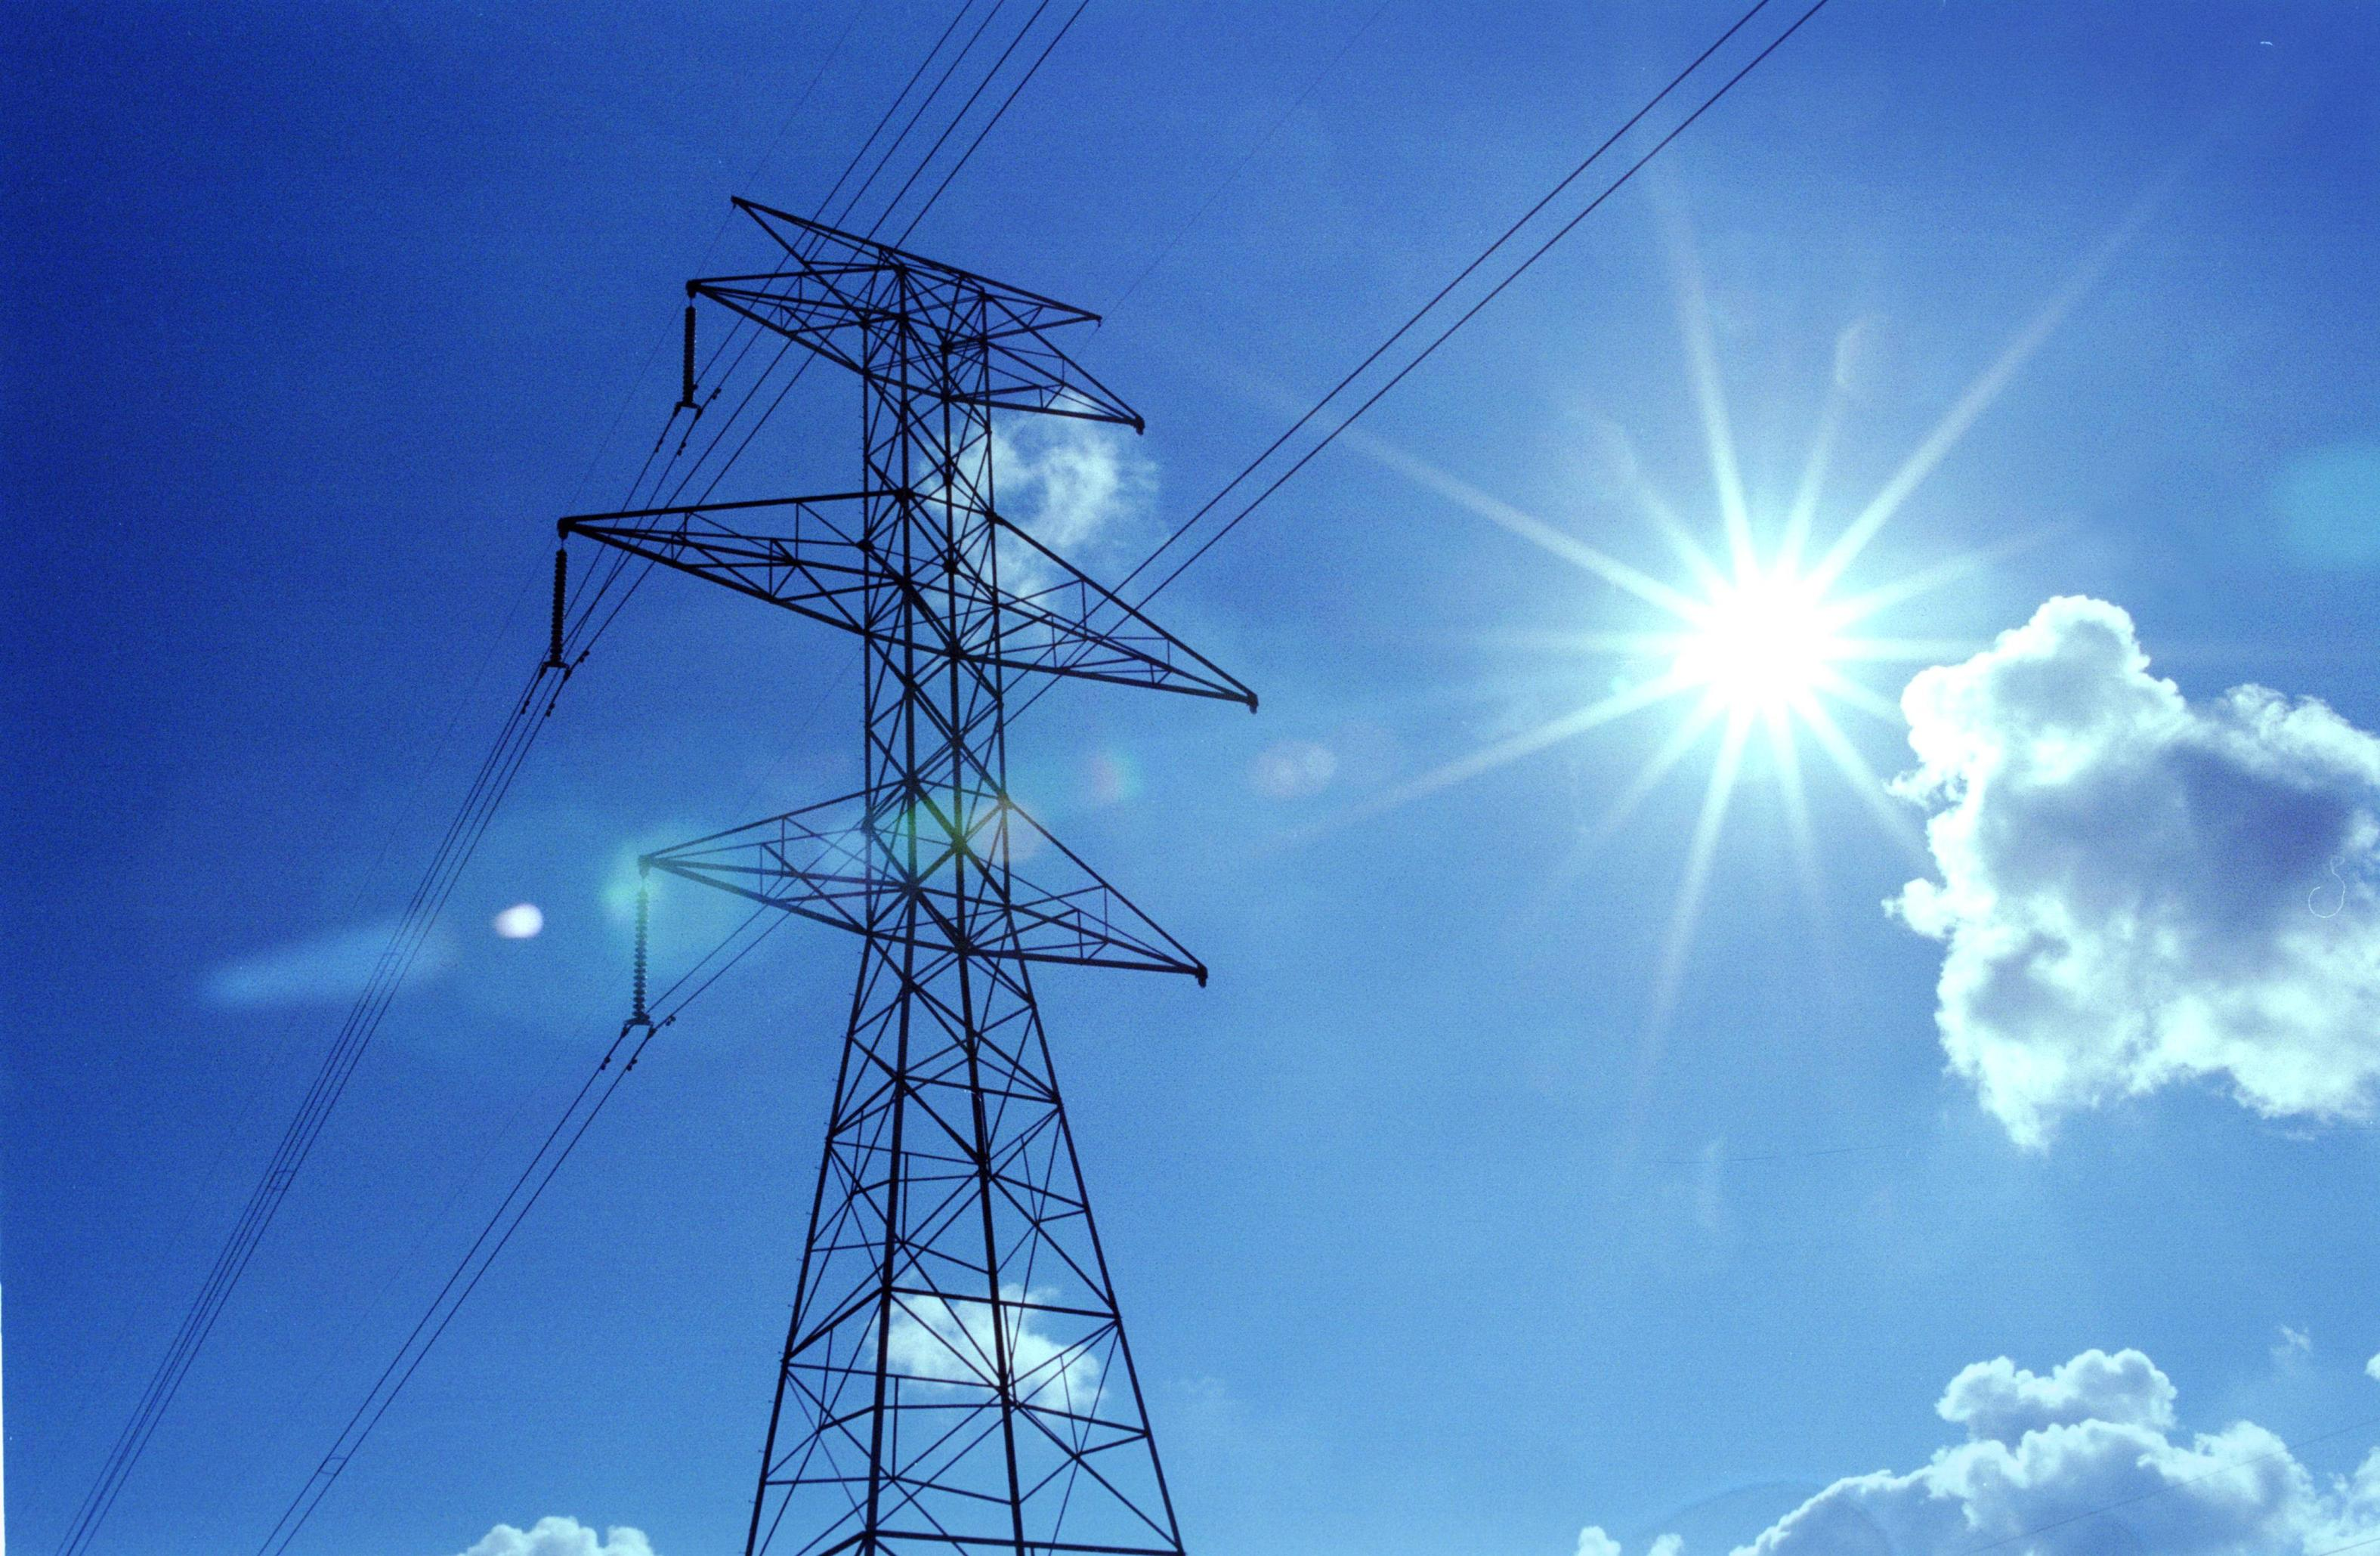
\includegraphics[width=1\linewidth]{./graphics/transmission1}
\caption{Overhead transmission line}
\end{figure}


The concept of electromagnetic waves has fascinated man for so many years that man has asked so many questions varying from "Why do stars twinkle?", to "Why do magnetic needles deflect?", and "Why does light travel from the sun when there is no medium between?"\newline

In modern-day, questions vary from "how do we have tv reception?" to "how do we have radio stations operating" to "how does a mobile phone work?", "why are certain things halted when they are kept inside a microwave". All these phenomena revolve around the concept of electromagnetic waves.\footnote{The concept of electromagnetic waves is virtually applied in almost all advanced technology.}\\

Electromagnetic waves can be divided into;
\begin{enumerate}
\item low frequency and high power
\item high frequency and low power
\end{enumerate}


In this course, we shall concentrate on the high-frequency and low-power properties of electromagnetic waves. Devices and phenomena like electrical machines, electrical power generators, transformers, and distribution of electrical energy fall into the category of low-frequency high power. Whereas modern systems, like mobile communication, radars, satellite, and optical fibres, fall into the high-frequency low-power category. So we are mainly going to investigate what happens as frequency increases in electromagnetic waves\footnote{When the frequency of a wave increases, the wavelength will decrease to compensate for this increment} and how they can be transmitted from one position to another without loss.\\

Electromagnetic waves see applications in many areas namely\footnote{The application of electromagnetic waves are not limited to this list but for this course, we streamline the application to these few.}:
\begin{enumerate}
\itemsep0em
\item Transmission lines and HF circuits.
\item Antennas.
\item Satellite communication.
\item Fibre-optic communication.
\item Radars.
\item Radio astronomy.
\item Electromagnetic Interference/Compatibility(EMI/EMC)
\end{enumerate}

We intend to investigate the behavior of time-varying electrical and magnetic fields especially when the frequency of operation is large. This investigation is going to be based on maxwell's four equations of electromagnetic waves\footnote{see chapter 17 for detailed expression of maxwell's equations}. However, as we proceed certain approximations can be used to investigate the same phenomenon in terms of voltage and current which are electrical circuits.\\

\begin{figure}[h]
\centering
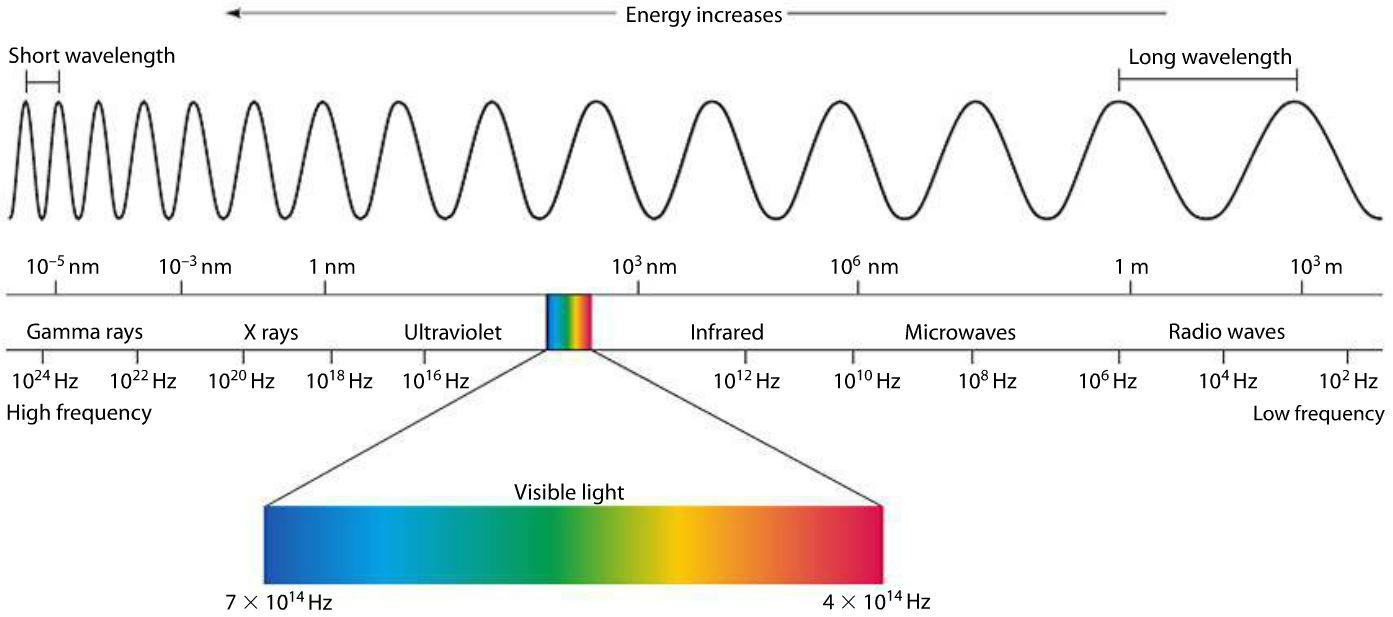
\includegraphics[width=1\linewidth]{./graphics/electromagneticspectrum}
\caption{The electromagnetic spectrum}
\label{fig:electromagneticspectrum}
\end{figure}

\textbf{Electromagnetic spectrum:} The word electromagnetic spectrum corresponds to any phenomenon which relates the time-varying signals and time-varying electric or magnetic fields \textit{electromagnetic spectrum shown in Figure~\ref{fig:electromagneticspectrum}}. Any wave no matter how small can be put in the category of time-varying electric or magnetic fields. The entire frequency range from very low frequencies to very high frequencies can be summarized as \textbf{radio frequencies}.\\

\section{Transmission lines and High-frequency circuits}

Depending on the frequency of operation, there are different media to transmit electromagnetic waves. When the frequency is between 30MHz to 300MHz, the coaxial cable is used for transmission of the wave, from 30GHz to 300GHz the structure used is called a waveguide and as the frequency goes high the media used is the optics fibre.

A question that comes to mind in electromagnetic wave transfer is "Why do we have to increase frequency?" If the major application of high frequency is in communication, then for transmitting more information we require large bandwidth. Since the frequency of operation is proportional to the bandwidth, by increasing the frequency of operation we increase the bandwidth and as such one can transmit more information on a given channel.
\begin{figure}[h]
\centering
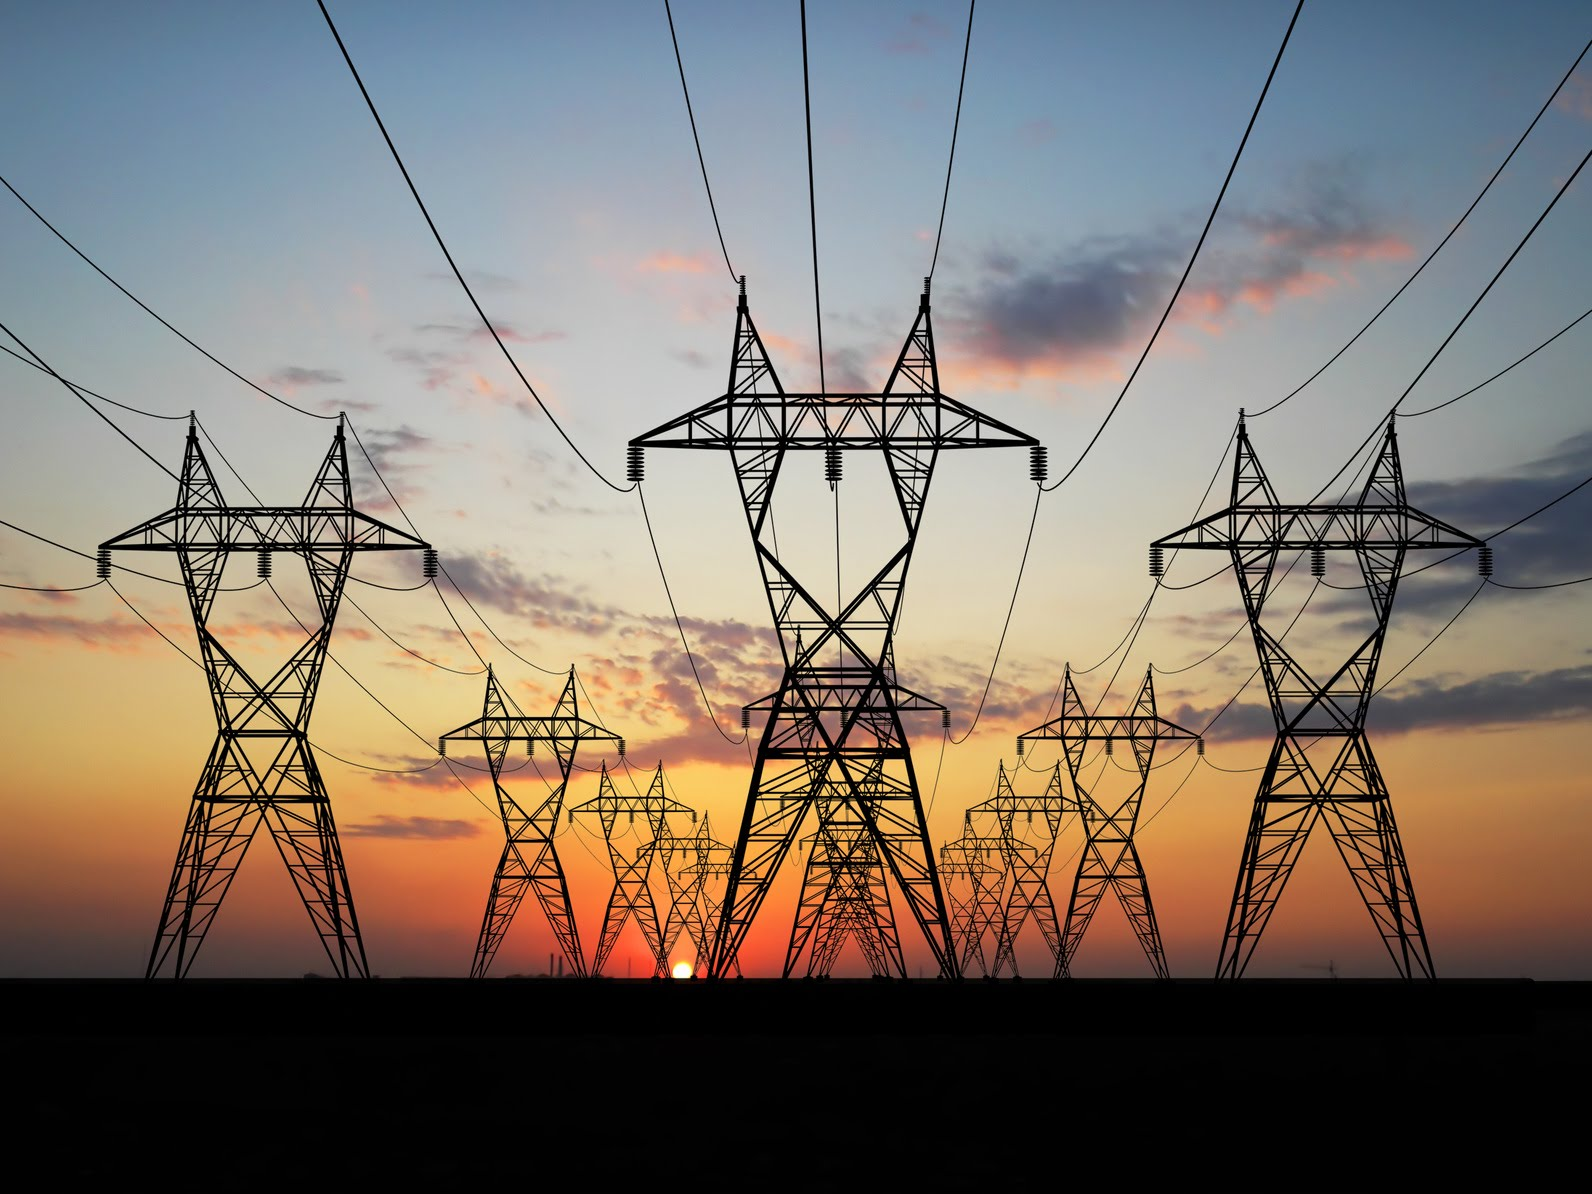
\includegraphics[scale=0.1]{./graphics/transmission2}
\caption{Power transmission line}
\end{figure}

\textbf{Transmission line:} In transmission lines, our main concern is how voltage and current would flow in a two-conductor system called a \textit{transmission line} and how losses occur during transmission \footnote{when the frequency of a wave increases its wavelength decreases and when the wavelength of the wire is comparable to the length of the transmitting media (length of the wire) the losses along the wire becomes too significant to ignore.}.

There are different types of transmission media and the application of this media is based on the frequency range of the signal. \begin{figure}[h]
\centering
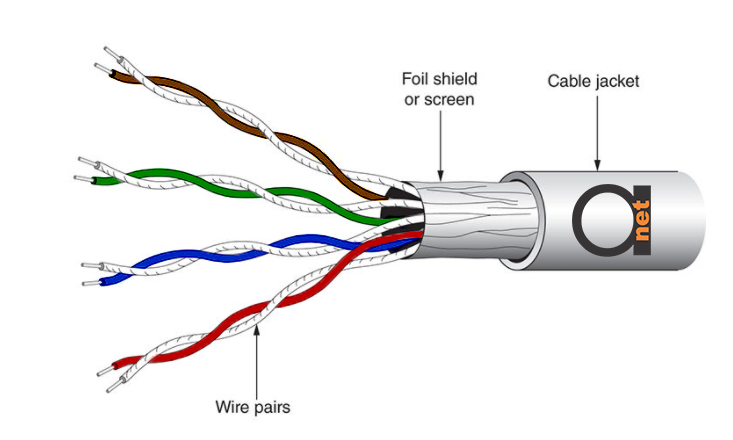
\includegraphics[width=1\linewidth]{./graphics/twistedpairs}
\caption{Twisted pair of wires}
\end{figure} 

\textbf{Twisted pairs:} They are point to point transmission lines\footnote{connections between two nodes or endpoints} (it is a balanced transmission line having voltages $v^{+}$ and $v^{-}$ connected at its terminals). An example of the twisted pairs is the telephone wires; it characterizes low data rate, high EMI and is lossy at Radio frequency.

\textbf{Coaxial cable:} For the coaxial cable we have an example in the LAN cable; it characterizes data rates of up to a few Mbps, low EMI and moderate loss.
\begin{figure}[h]
\centering
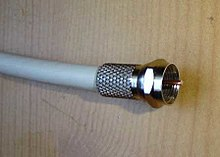
\includegraphics[scale=0.4]{./graphics/coaxialcable}
\caption{Coaxial cable}
\end{figure}

\textbf{Wave guides:} These are hollow circular or rectangular pipes and they are used when the frequency becomes high in other to reduce losses. 

Inside the hollow metal conductor, an electromagnetic wave can propagate and here rigorous analysis of electromagnetic wave propagation is carried out to help find out what the field distribution would look like and how much energy loss will take place inside.
\begin{figure}[h]
\centering
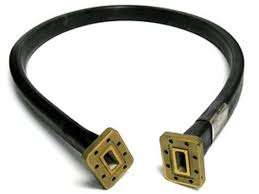
\includegraphics[scale=0.4]{./graphics/waveguide2}
\caption{Wave guide}
\end{figure}

\section{Antennas}
\begin{figure}[h]
\centering
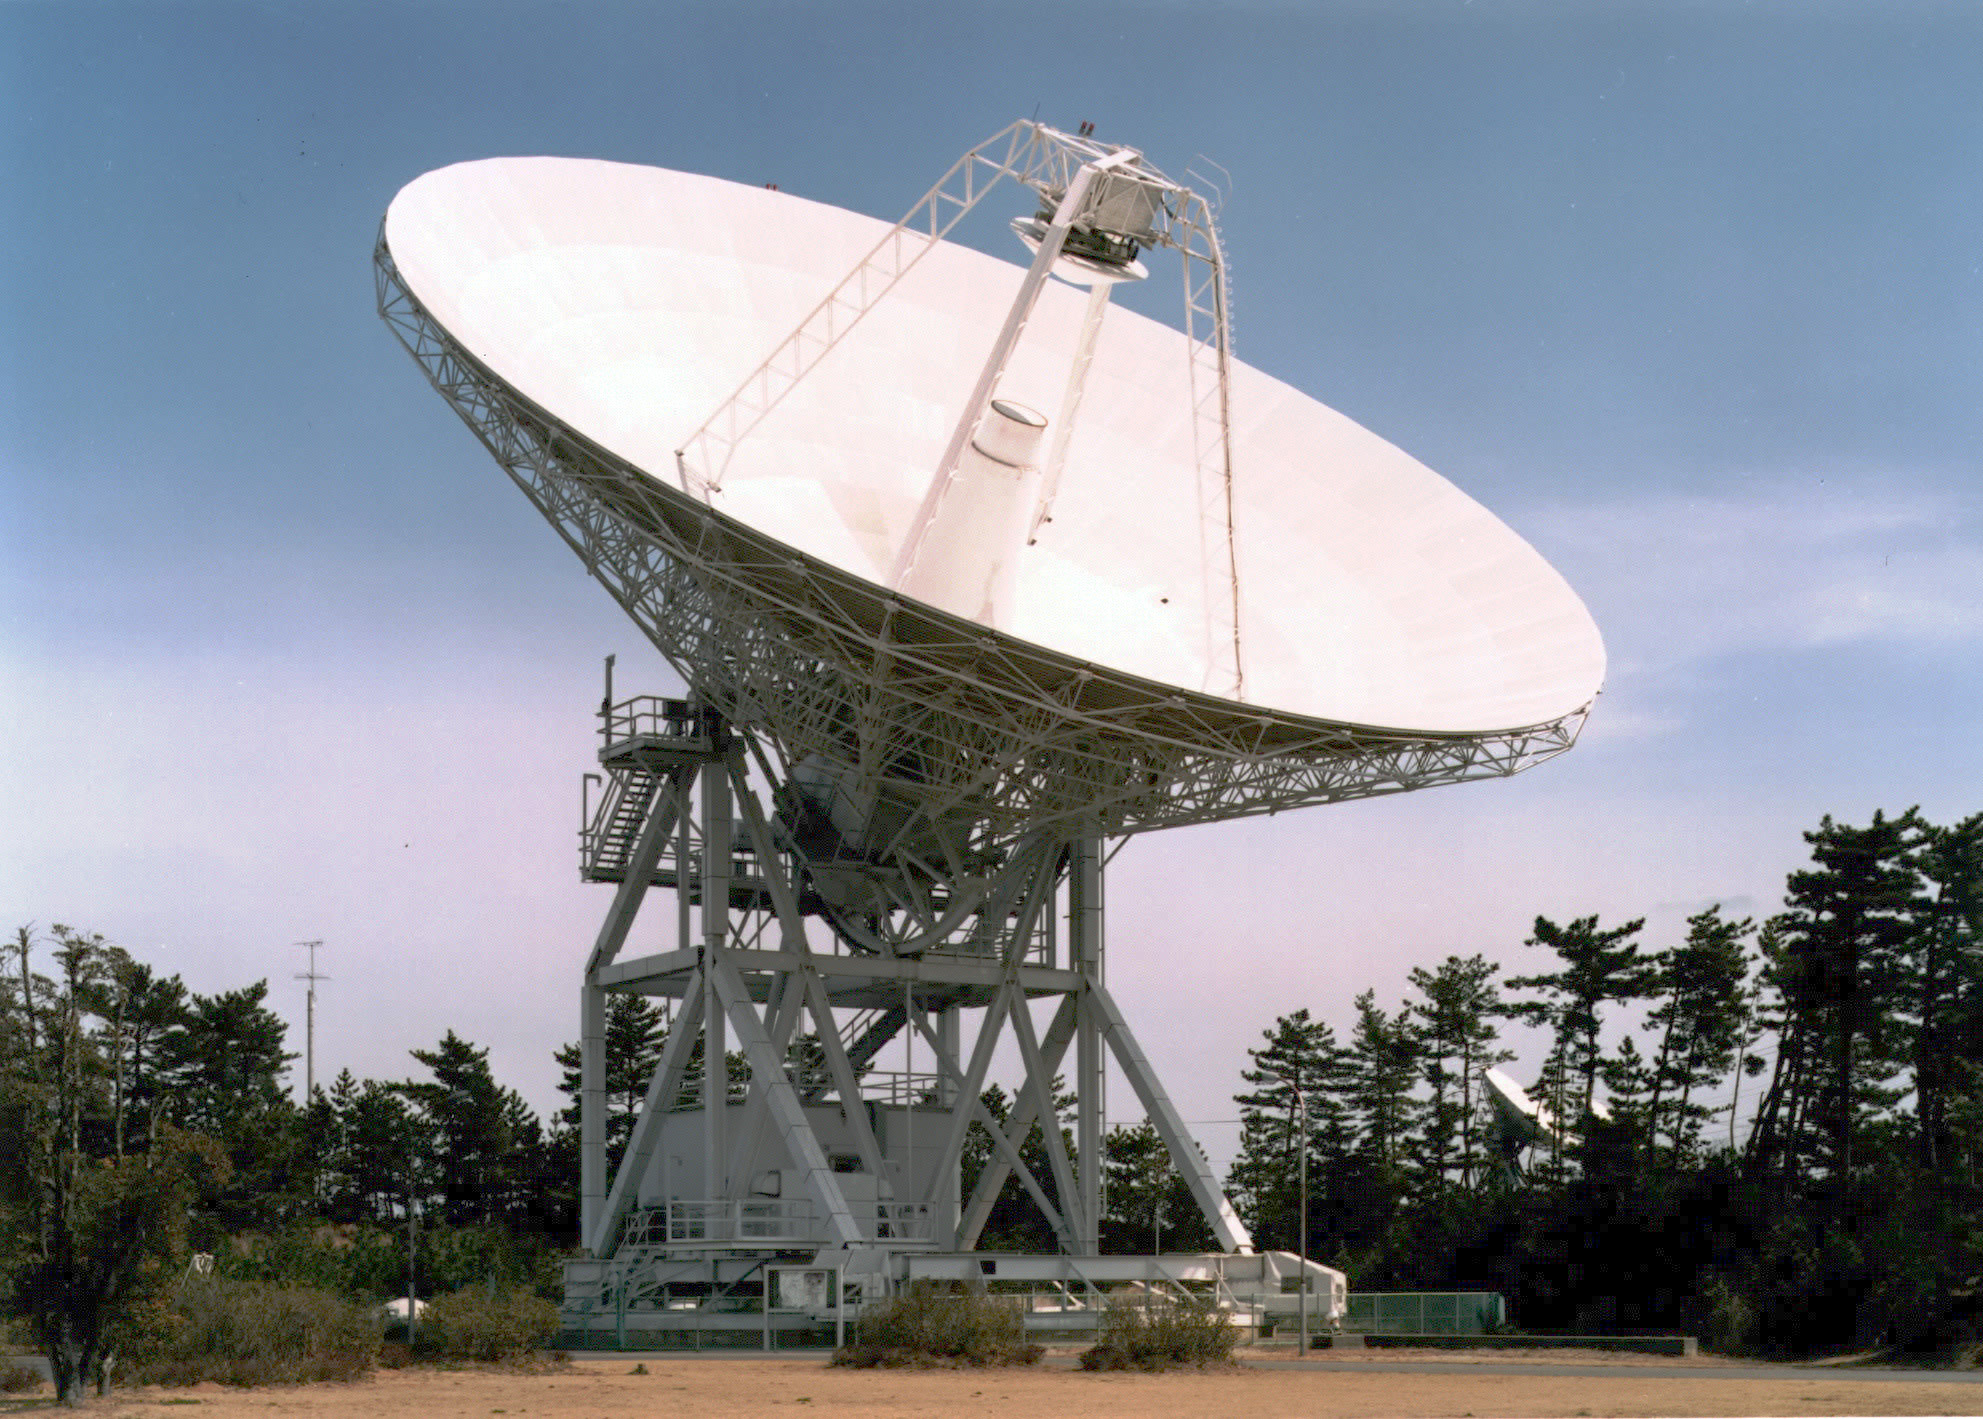
\includegraphics[scale=0.4]{./graphics/spcaceantenna}
\caption{Parabolic dish antenna}
\end{figure}
An antenna is a device which can transmit electromagnetic energy into space and also can receive electromagnetic energy coming from space. An example is the parabolic dish antenna, signals coming from a point are like parallel rays when it gets to the parabolic dish antenna the rays converge to a focal point called the feed from there they get processed into an electrical signal.\\

An antenna is a device which separately puts radiation in the desired direction. A simple antenna structure may not necessarily provide the desired characteristics of modern-day smart antenna systems where radiation characteristics can be automatically changed to maximize the reception of the signal.\\

Other more advanced antenna systems referred to as the \textbf{smart antennas} can selectively push the radiation in the desired direction. There are two types of smart antennas which are the \textbf{adaptive array} and \textbf{switched beam systems}.\\

\textit{\textbf{adaptive array}}
This antenna steers the beam in the direction of the user/transmitter while simultaneously nulling interfering signals.
\begin{figure}[h]
\centering
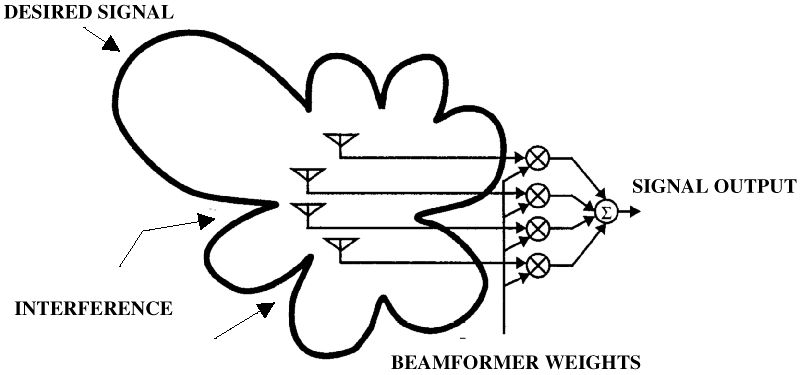
\includegraphics[scale=0.3]{./graphics/fh06_02}
\caption{Adaptive array system}
\end{figure}

\textit{\textbf{switched beam antenna}} has multiple beams which can be switched depending on the area an observer is situated. A signal can be transmitted or received from that zone. Therefore, depending on the requirement of the system a beam is selected hence the name switched beam.
\begin{figure}[h]
\centering
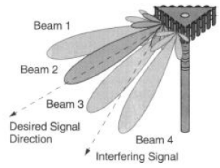
\includegraphics[scale=0.7]{./graphics/switchedbeam}
\caption{Illustration of a switched beam antenna}
\end{figure} 

\section{Satellite communication}
A satellite is an object that is placed above the earth's surface. The satellite station on the earth's surface is usually called the earth station which transmits signals from the earth to satellites and also receives signals from the satellite to the earth. Certain frequency bands are assigned for satellite communication. Satellite communication is a point-to-multi-point system.
\begin{figure}[h]
\centering
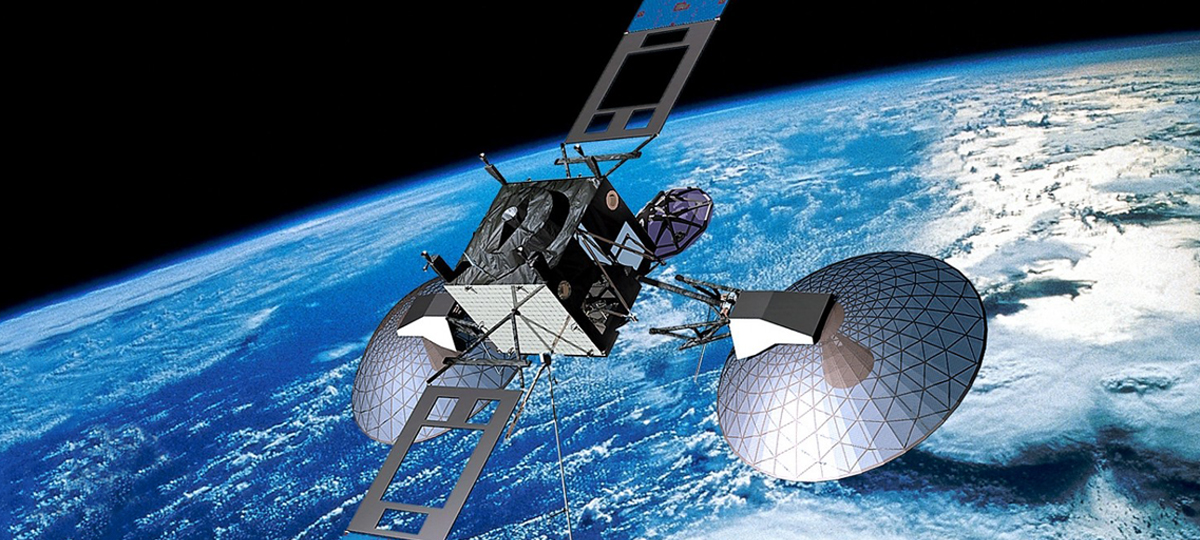
\includegraphics[scale=0.2]{./graphics/satellite}
\caption{Space satellite}
\end{figure}

The whole propagation of the electromagnetic wave and proper placing of radiation in the direction towards the earth is achieved with the principles of electromagnetic waves. Satellite communication has a large delay because of the turnaround trip taken from the earth station to the satellite and the satellite back to the earth station.

\section{Fiber optics communication}
\begin{figure}[h]
\centering
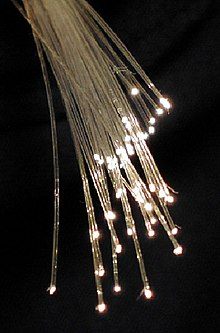
\includegraphics[scale=0.4]{./graphics/opticalfiber1}
\caption{Optical fiber}
\end{figure}

Knowledge of electromagnetic waves is required to investigate the propagation of light inside a fibre optic material. Fibre optic cable is made up of very thin hollow glass strands in which light is reflected internally. As the light propagates inside the optical fibre, the signal gets distorted and hence the knowledge of electromagnetism is needed to know how the signal gets distorted.

\section{Wireless communication}

Wireless communication is used in cell phones and most modern systems like home entertainment systems using Bluetooth speakers, laptops using a wireless method to connect to routers and so on. All these work on the principle of electromagnetic waves.
\begin{figure}[h]
\centering
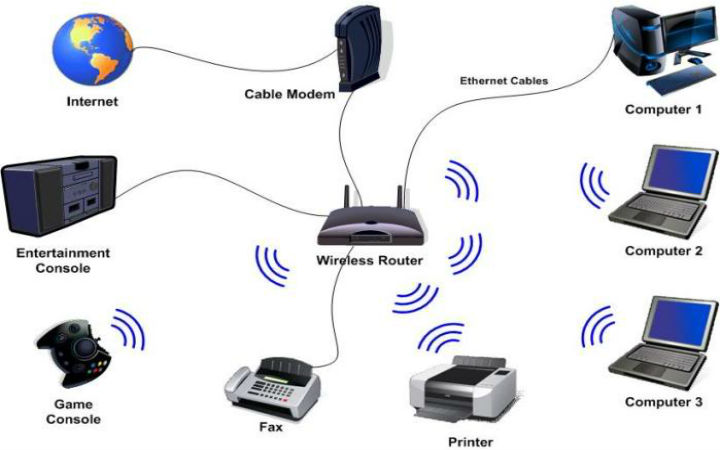
\includegraphics[scale=0.3]{./graphics/Expert-support-for-wireless-communication-projects}
\caption{Wireless connection od devices}
\end{figure}
\section{Cellular communication} 

In cellular communication, we have the base station from where the signals are transmitted, all users located inside are called a cell. Any mobile call made goes from the handset to the base station in that sector and then goes to the desired handset in the sector.
\begin{figure}[h]
\centering
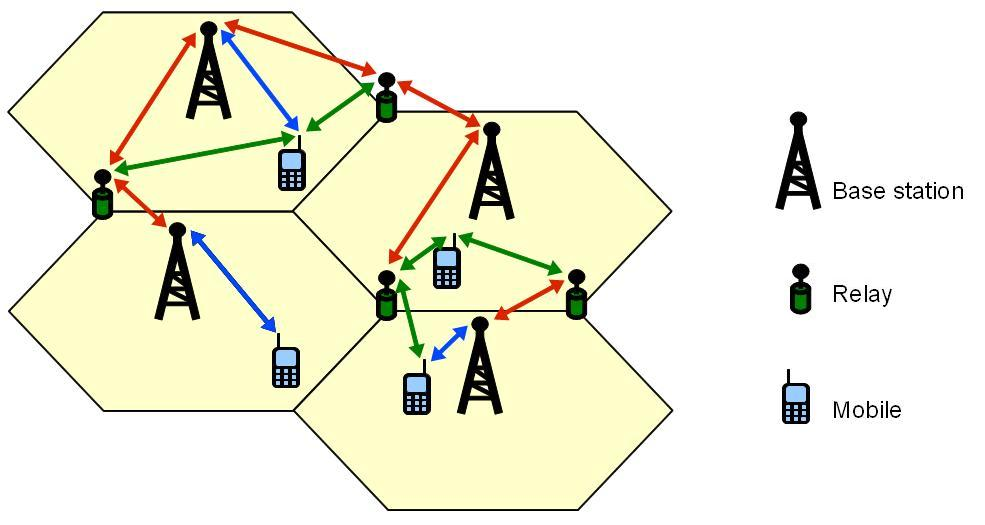
\includegraphics[scale=0.3]{./graphics/RR_sada_fig1}
\caption{Cellular communication}
\end{figure}

It is observed that a cell phone user has signals from multiple paths all coming to his cell phone\footnote{Relays are used to transmit and receive information between the base station and mobile when they are too far away to send the information to each other directly}. The mobile does not only get signals coming directly from the base station, but It also encounters signals due to reflection from associated objects. As a result of interference of these signals which can either be constructive or destructive, the final signal transmitted/received is altered. 

When there is constructive interference, a strong signal strength is observed and when the interference is destructive, a weak signal strength is observed.
The gradual weakening of a signal due to destructive interference is called \textit{fading}. To understand fading phenomenon a good knowledge of electromagnetic waves is required.\\\\

\textbf{Antennas and antenna systems for cellular communication}: To avoid fading phenomena, antennas in the mobile use sectioned propagation pattern. This implies that the cell phone gets its signal from the base station directly while minimizing signals from paths not in the direction of the base station of the antenna. A good knowledge of electromagnetic waves is required to design this system.
\begin{figure}[h]
\centering
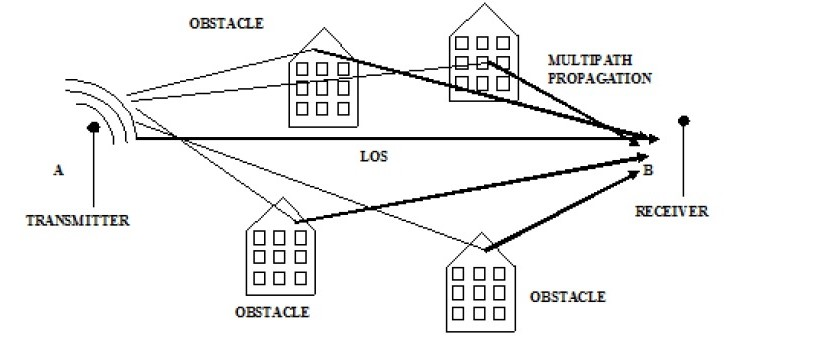
\includegraphics[scale=0.4]{./graphics/rod}
\caption{Illustration of signal inference}
\end{figure}
\section{Radar and remote sensing}
In radar altimetry, electromagnetic waves are used for finding the distance of an object from the point to the antenna. The antenna is excited with an electromagnetic pulse and the dish beams parallel waves downwards. This beam is reflected from the earth's surface back to the dish. The dish converges the received signal back to the antenna, Resulting signals are now processed in the detector, see figure 1.15.
\begin{figure}[h]
\centering
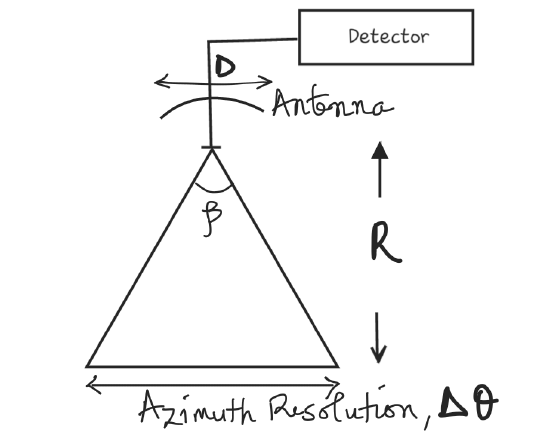
\includegraphics[scale=0.6]{./graphics/New}
\caption{Radar Altimetry}
\end{figure}

where the resolution $\Delta \theta = \frac{\lambda}{D}$\footnote{The implication of this equation lies in the size of the antenna. To get a high resolution the size of the antenna would be large}, $\lambda$ is the wavelength of the beam and $D$ is the size(length) of the antenna. 
From the time delay($\frac{C t}{2}$) of transmission to the reception of the electromagnetic pulse. The distance travelled by the beam can be estimated and also if the object is moving in the radial direction, there would be a frequency change between the signal transmitted by the antenna and the signal reflected(Doppler shift) and from this result the velocity of the object can be estimated. The radar essentially uses the electromagnetic pulse to find the distance and the velocity of an object.\\

\textbf{The monostatic radar equation}
\begin{figure}[h]
\centering
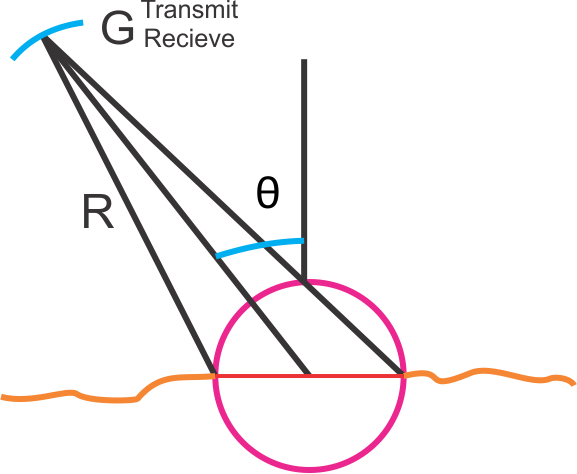
\includegraphics[scale=0.4]{./graphics/new1}
\label{fig:new1}
\caption{}
\end{figure}
\begin{center}
$p_{r}= \frac{\lambda^{2} G \delta \sigma A}{(4\pi)^{2}R^{2}}$
\end{center}

From Figure~\ref {fig:new1}, where $p_{r}$ is the received power, the signal goes from the radar to the object and is again received by the antenna in the radar. The magnitude of the received signal can be calculated and this requires a good knowledge of the ability to model the propagating environment and a good modelling of the scatterer from which the energy is going to be reflected.\\

\begin{figure}[h]
\centering
\includegraphics[scale=0.5]{./graphics/Radarlocator}
\caption{radar locator}
\label{fig:radarlocator}
\end{figure}

In Figure~\ref{fig:radarlocator}, we can see the various objects detected by the radar(represented by a green dot). The green radial line represents the transmitting beam\\

\textbf{Side looking airborne radar(SLAR):} is a radar technique used for remote sensing, it is an imaging radar\footnote{Imaging radar provides its light to illuminate an area on the ground and takes the picture at radio wavelengths} mounted on a moving object like the aircraft pointing perpendicular to the direction of flight (hence side-looking). A squinted (non-perpendicular) mode is possible also. SLAR can be fitted with a standard antenna (real aperture radar) or an antenna using synthetic aperture(this would be discussed in the next section). The platform of the radar moves in direction of the x-axis. The radar looks with the looking angle $\theta$ (or so-called off-nadir angle).\\

The microwave beam is transmitted obliquely at right angles to the direction of flight illuminating a swath.\\
Swath width refers to the strip of the Earth's surface from which data are collected by a side-looking airborne radar. It is the width of the imaged scene in the range dimension. The longitudinal extent of the swath is defined by the motion of the aircraft with respect to the surface, whereas the swath width is measured perpendicularly to the longitudinal extent of the swath. Range refers to the across-track dimension perpendicular to the flight direction, while azimuth refers to the along-track dimension parallel to the flight direction\footnote{This technique is mostly used in aircraft}.\\

\textbf{\textit{To measure the azimuth resolution}}\\
The SLAR is primarily a real aperture radar. This requires a reasonably large antenna for adequate angular resolution. The azimuth resolution, $ Ra $, is defined as
\begin{center}
$R_{a}=\frac{H \lambda}{L cos\theta}$
\end{center}
$ H $ is the height of the antenna(height of the airplane)\\
$ D $ is the geometric length of the antenna,\\
$\lambda$ is the wavelength of the transmitted pulses, and\\
$\theta$ is the incidence angle
\begin{figure}[h]
\centering
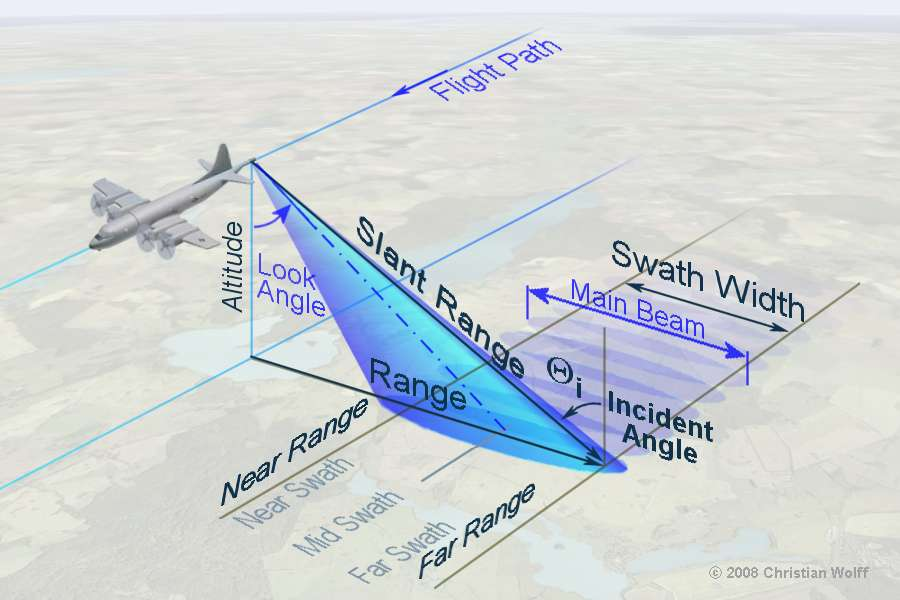
\includegraphics[scale=0.2]{./graphics/SLAR2}
\caption{Diagram expressing the SLAR}
\end{figure}

The equation shows, that increasing altitude decreases the azimuthal resolution of SLAR. A very long antenna (i.e., large D)\footnote{For this book, $D$ is the size of the antenna. hence the statement "large D", since the length ($L$) of an object is a function of the size ($D$)} would be required to achieve a good resolution from the aircraft. Synthetic Aperture Radar (SAR) is used to acquire higher resolution.\\

\textit{\textbf{To measure the cross-track resolution }}\\
At all ranges, the radar antenna measures the radial line of sight distance between the radar and each target on the surface. This is the slant range distance. The ground range distance is the true horizontal distance along the ground corresponding to each point measured in the slant range. The cross-track resolution, $R_{r}$, is defined as:  
\begin{center}
$R_{r}=\frac{c_{0} t_{p}}{2 sin\theta}$
\end{center}
$c_{0}$ is the speed of light\\
$t_{p}$ is the pulse duration of the transmitter and\\
$\theta$= incidence angle

\begin{figure}[h]
\centering
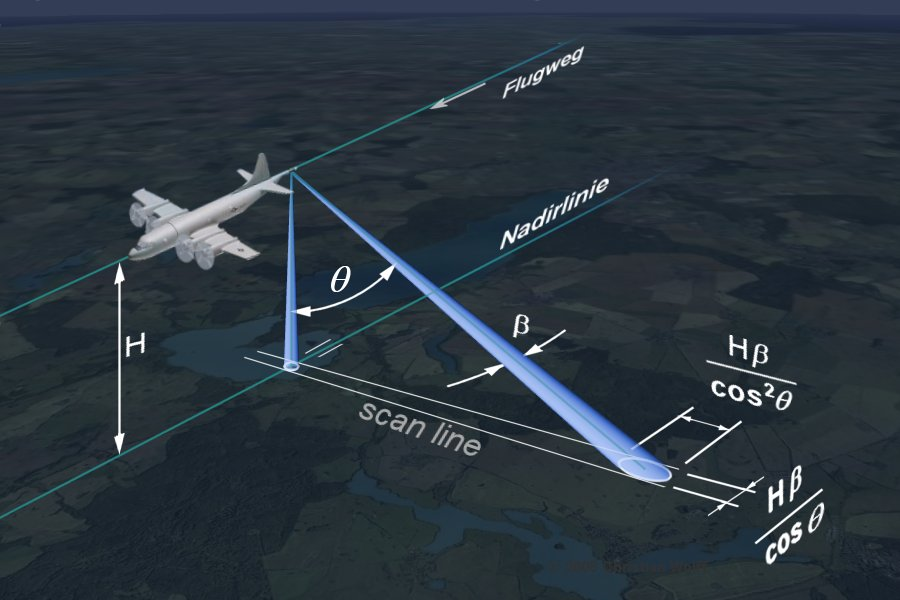
\includegraphics[scale=0.2]{./graphics/SLAR-resolution}
\caption{Diagram expressing the SLAR}
\end{figure}
\textbf{Synthetic aperture radar(SAR):} To improve the resolution in remote sensing, a technique called the synthetic aperture dish is used. For an antenna like a parabolic dish, the angular resolution is given as the wavelength divided by the size\footnote{For a parabolic dish antenna the diameter 'd' is used instead of length 'L'.See footnote 11} for the antenna, $\Delta \theta = \frac{\lambda}{D}$. To get a fine resolution for the image in remote sensing, a very large aperture D is required. A large D cannot be easily created especially in moving vehicles and aircraft.\\

A technique where the antenna is small but the vehicle moves and as the vehicle moves, the reflection information is stored after all the refection information is collected from different locations, then data processing can be done to get an angular resolution which will correspond to the total distance traveled by the vehicle. This technique is known as the \textit{synthetic aperture radar}.
\begin{figure}[h]
\centering
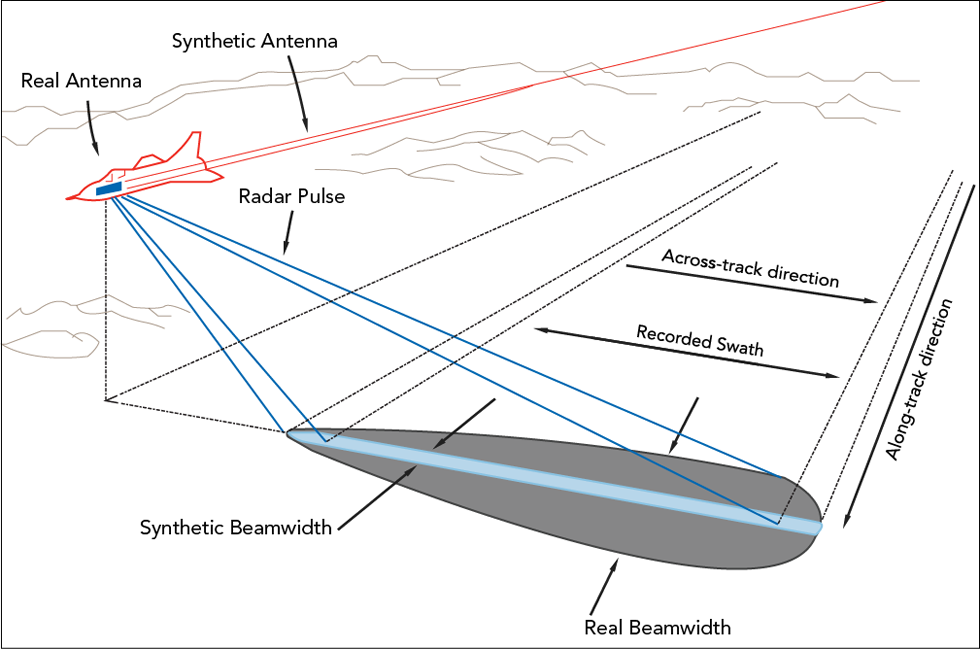
\includegraphics[scale=0.3]{./graphics/sar2}
\caption{Diagram expressing the SAR}
\end{figure}

\textbf{SAR features}
\begin{enumerate}
\itemsep0em
\item very high linear resolution independent of the range
\item requires a source with higher coherence
\item image is on the range-doppler coordinate grid
\item requires a large data processing
\item geometric and ratio metric distortions
\item speckle noise
\end{enumerate}

\section{Radio astronomy} 

A typical radio telescope is shown below with a passive receiver. In this case, no signal is transmitted but the signal is received.\\
\begin{figure}[h]
\centering
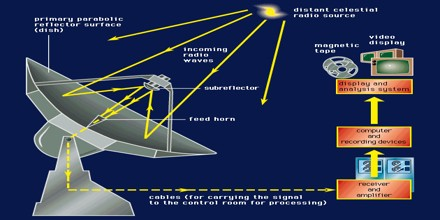
\includegraphics[scale=0.5]{./graphics/Radio-Telescope-0}
\caption{Radio telescope}
\end{figure}

The frequency of the signals is converted, detected and processed. With a radio telescope, we would like to get an image of the sky with as large a resolution as possible.

$\frac{\lambda}{D}$ comes into the picture and to get a very fine resolution of the image of the sky, a very large telescope would be needed.

Producing a very large telescope is difficult so we use the aperture synthetic technique as it was used on radars. In this method we use a set-up of antennas, for example, if the dish in each array is of the order of $ D = 25m $ and the total spread of the antennas of the order 21km. Therefore, we get an effective aperture through each antenna that has an aperture of only 25m.

\section{EMI/EMC}

\textbf{EMI} is electromagnetic interference.
Firstly, let us investigate how a high-frequency device would create interfering signals and then what ways in which the interference can be reduced.

For example, you may get interference on our radios, whenever somebody starts a car or a motorcycle in the vicinity, because starting a car or motorcycle involves sparking and because of that spark, you get electromagnetic interference which is picked up by the radio antenna and you get disturbance on your radios. It is essential to investigate the technique by which the interferer can be reduced or the mechanism by which the devices can be isolated. This technique is called \textit{\textbf{shielding}}.\\

\textbf{EMC} is electromagnetic compatibility. Today, whenever we design electromagnetic gadgets or electrical devices it is mandatory to make them electromagnetically compliant so it does not create additional electromagnetic interference which will affect the other systems.

The figure below describes the whole concept of EMC both causes(natural or man-made) and solution(shielding and other techniques).
\begin{figure}[h]
\centering
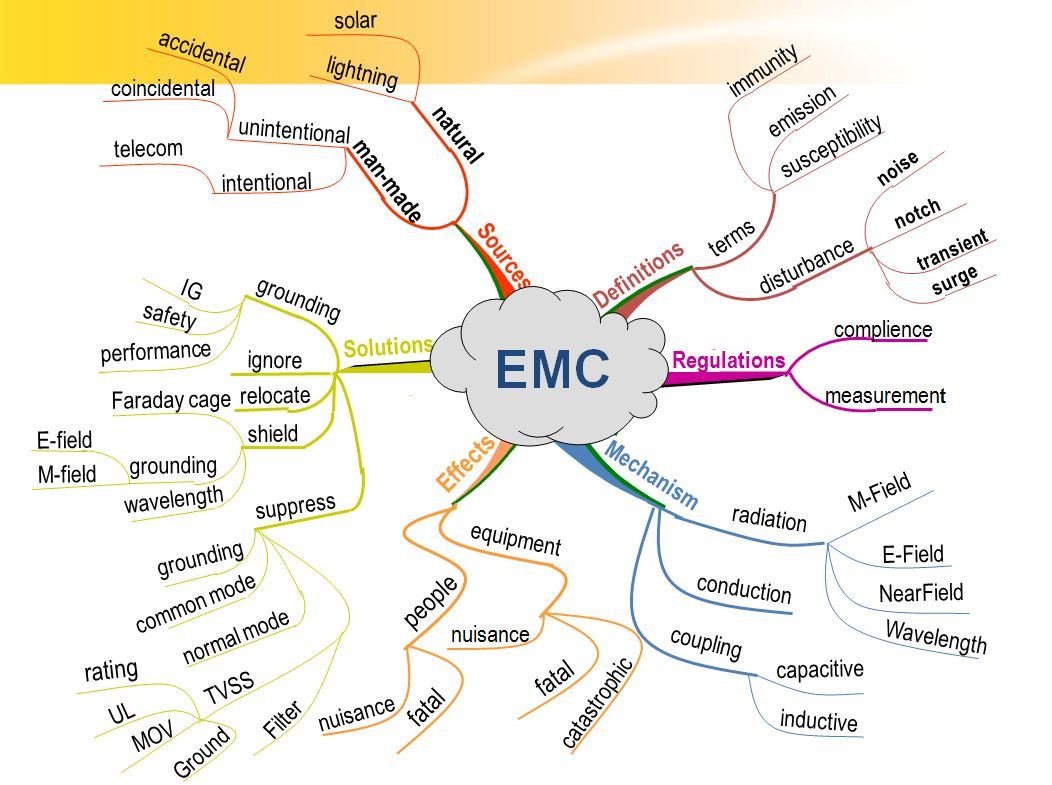
\includegraphics[scale=0.35]{./graphics/634771461726914062}
\caption{Electromagnetic Compatibility}
\end{figure}

%\chapter{Transmission lines}
Transmission lines are special cases of electromagnetic waves that deal solemnly with time-varying voltage and current. In the previous chapter, emphasis was placed on the subject of electromagnetic waves that deal with electric and magnetic fields that vary with time. Transmission lines are unique because the concept of voltage and current are still very much valid.

In this chapter, we will still be working with the concept of voltage and current which everyone is familiar with and then gradually introduce the concept of space into the circuit analysis. 

\section{Structures of transmission lines}
Transmission lines can best be defined as a medium of power transfer from one point to another. This transmission is done through a variety of structures, some of which are explained below;

\subsection{Co-axial cable}	
\begin{figure}[h]
\centering
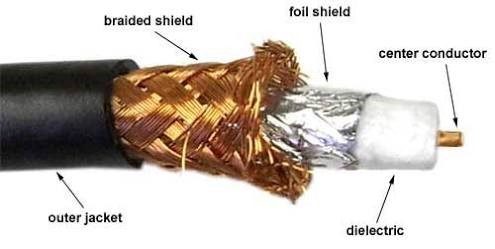
\includegraphics[scale=0.65]{./graphics/coaxial}
\caption{Co-axial cable transmission line}
\end{figure}
 In this particular setup, there’s an inner and outer conductor and voltage is applied between the inner and outer conductor thus energy will be propagated along the length of the structure.
\subsection{Parallel wire transmission lines}
 \begin{figure}[h]
\centering
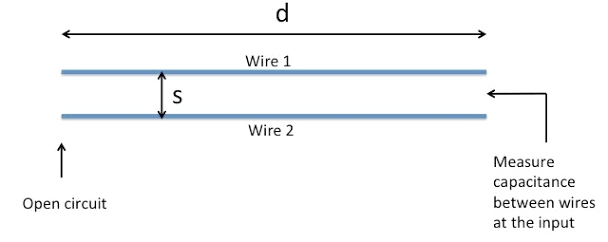
\includegraphics[scale=0.4]{./graphics/twowire}
\caption{Parallel wire}
\end{figure}
This setup is quite the simplest. We simply have two separate conductors hence when voltage is applied at both ends, energy flows.
\subsection{Microstripline}
\begin{figure}[h]
\centering
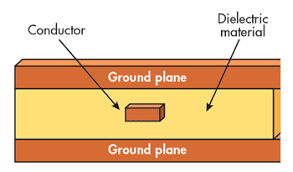
\includegraphics[scale=0.7]{./graphics/micro}
\caption{Microstripline }
\end{figure}
The microstrip line is a transmission line geometry with a single conductor trace on one side of a dielectric substrate and a single ground plane on the other side.
\subsection{Unbalanced}
\begin{figure}[h]
\centering
\includegraphics[width=1\linewidth]{./graphics/Unbalanced}
\caption{ Unbalanced }
\end{figure}
 In this structure we have a conducting rod above a ground surface and voltage is applied between the rod and the ground surface hence power is transmitted efficiently along the structure.
\subsection{Stripline} 
Also known as differential-stripline. The structure is made up of two parallel conductors enmeshed in a dielectric that has conducting surfaces at the top and bottom which are grounded while the voltage is applied between the two conductors.
\begin{figure}[h]
\centering
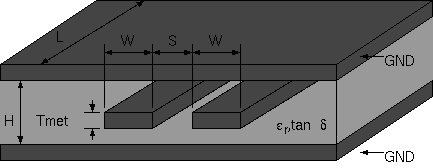
\includegraphics[width=1\linewidth]{./graphics/stripline}
\caption{ Stripline}
\end{figure}

The summary of all we have been discussing is that we are having a two-conductor system, hence when voltage is applied between them. Because it is a time-varying voltage current that flows through the system.

All the structures can be represented by a simple two-conductor system and this is also done for transmission line analysis where we ignore the structure and simply treat it as a two-conductor system, at one end we apply an energy source and at the other end, we apply a load and then carry out analysis from the source to the load.

\section{Concept of transit time effect }
Circuit laws like Kirchhoff’s law, are limited to low-frequency circuits where we only take note of the value of the electrical components, i.e. For a circuit that comprises resistors, capacitors and inductors, only their values are needed for the circuit analysis.

However, as frequency increases, the signal value changes significantly. A good example is shown in Figure~\ref{fig:first}.

\begin{figure}[h]
\centering
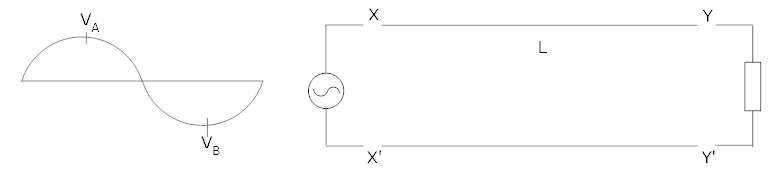
\includegraphics[width=1\linewidth]{./graphics/first}
\caption{circuit diagram of a transmission line}
\label{fig:first}
\end{figure}

At some instant, $ V_{A} $ is applied at X, and when L is sufficiently small relative to the length ($  \lambda = \text{wavelength} $). We assume that $ V_{A} $ appears at Y from X almost instantaneously.

But if $f$ (frequency) of the signal is very high, $\lambda $ gets very small and so is far less than L, hence  $  V_{A} $ applied at X takes some finite time before It gets to Y as $  L\gg \lambda $ (high frequency). Therefore $  V_{Y} $ is not always $  V_{X} $.

In transit time effect one can realise that $ \lambda $  approaches L and so it is very likely that $ V_{X} \neq V_{Y} $, but when $  \lambda \gg L  $ (for low-frequency circuits) the sinusoidal wave changes slowly so that we can assume it is constant across the entire L.\\
The finite time it takes the voltage at X to appear at Y is called transit time.
\begin{align}
 t_{r} = \frac{L}{v}\ \ \ \ \ \ (\text{Transit  Time})
\end{align}
$v$ is the velocity of the signal. So when a time-varying signal is applied at X, it requires a finite time to travel from X to Y.  $ V_{A} $  at X will not remain constant as it is a time-varying sinusoidal so that in the transit time it takes $ V_{A} $ to appear at Y, $ V_{A} $ would have changed to another value say $ V_{B} $, so when a voltage at Y is $ V_{B} $ say, the voltage at X is $ V_{A} $. In other words, there is a potential difference between X and Y. This difference is related to the length of the cable, the more the length the more the difference. With L very small, $ V_{x} $ is close to $ V_{y} $ as the points A and B will be close to each other and the voltage difference will not be substantial. The important thing here is no matter how small the length we take, there will always be that voltage difference $ V_{x} – V_{y} = 0 $ if $ L \rightarrow 0 $.

As we increase the frequency, the role of the transit time effect becomes more and more important. So now to the big question; \textit{When do you neglect transit time effect and when do you incorporate it in your design?}

If $ V_{x} – V_{y} $ is small, the transit time effect can be neglected otherwise it should be taken into consideration. Generally, if  $ t_{r} \ll T $ (period of signal), neglect transit time effect but if $ t_{r} $ is comparable to T (signal period), then we have to incorporate the effect of transit time in other words, when carrying out circuit analysis, the size of the structures will play a role in the analysis.
$$ T \gg t_{r}\ \ \ \ \ \ (\text{neglect transit time})$$\\\\
 Recall, T = $   \frac{1}{f}  $, $ t_{r} = \frac{L}{v} $ and $ \lambda = \frac{v}{f} $\ \ \ \ \ \ hence; 

if \hspace{0.05in}  $ \frac{1}{f} \gg \frac{L}{v} $ or $ \frac{v}{f} \gg L $ \\\\
Thus, $ \lambda \gg L $ \ as a result, the transit time effect is neglected.

\section{Analysis of Transmission line}
In low-frequency analysis, there is just a circuit size that fits all values like saying R= $ 0.1\Omega $, L=0.1H and C = $ 0.1\mu F $, unlike in high frequency where we have $ 10\Omega $ resistor of 1cm, 10cm and 100cm lengths which will cause each of the circuit to behave differently because of the non-uniform length when transit time effect is considered.

However, we still want to use the basic laws that we are familiar with for low frequency. The approach of this law will break the\textbf{ LUMPED ELEMENT} into \textbf{DISTRIBUTED ELEMENT} and also have per unit element value for each of the elements. The division of each circuit element in space is done in such a way that L is infinitesimally small so that the circuit laws at low frequency can apply within two nodes created by the division.\\

Transit time cannot be neglected for a two-conductor wire but when a small quantity in length is broken down into very Lineal elements of $ \Delta x $ with  $  \Delta x \rightarrow 0 $. The transit can be neglected as $ L \gg \Delta x $ and so the circuit laws of low frequency can be applied to the arbitrary nodes separated by $ \Delta x $ length. \\
In the circuit, we should have resistance, capacitance and inductance stated in total value, instead, we have resistance, inductance and capacitance all per unit length.

The relationship between voltage and current is valid for high frequency like that of low frequency as $ \Delta x  \rightarrow 0$ (infinitesimally small). Hence, this solves for voltage and current of a transmission line in the presence of the transit time effect.\\
\begin{figure}[h]
\centering
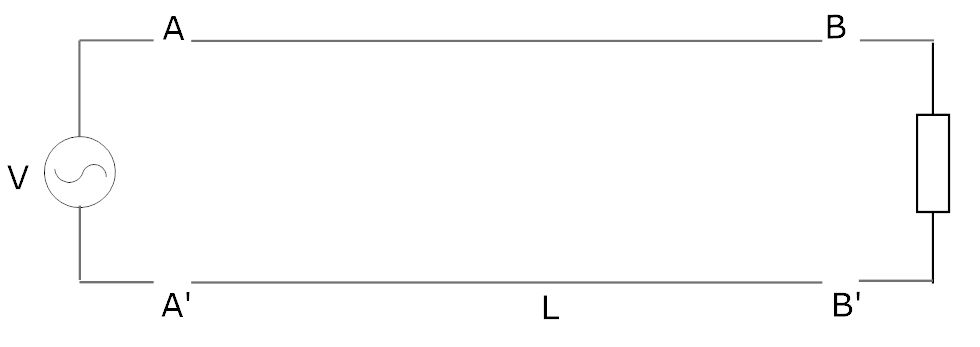
\includegraphics[width=1\linewidth]{./graphics/second}
\caption{simple circuit diagram of a transmission line}
\end{figure}	

In the circuit above, there is a voltage difference between both ends because of the transit time effect but we do not know why there is a voltage difference.

We all know that as frequency increases in the circuit, the two conductors have both electric and magnetic fields induced as shown below: 

\begin{figure}[h]
\centering
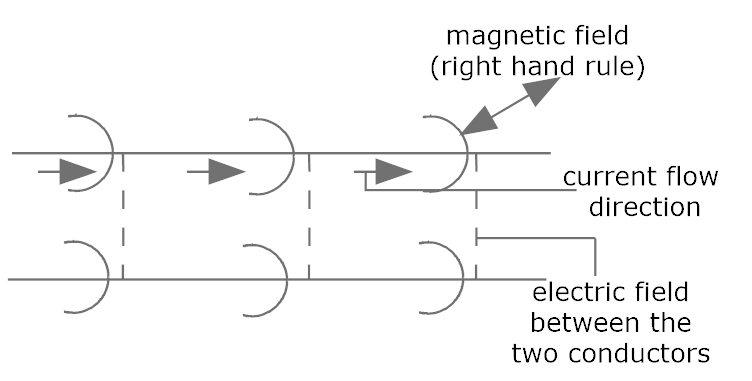
\includegraphics[width=1\linewidth]{./graphics/third}
\caption{transmission line circuit showing both electric and magnetic fields}
\end{figure}

So when the magnetic field is linked with current an inductance is produced while the electric field between the two conductors with air as dielectric gives a capacitor.

\begin{figure}[h]
\centering
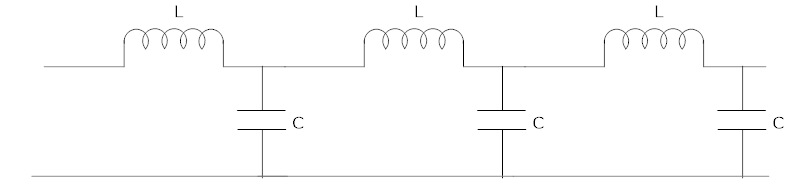
\includegraphics[width=1\linewidth]{./graphics/fifth}
\caption{distributed inductance and capacitance in transmission line circuit}
\end{figure}
The inductance and capacitance produced are distributed along the length of the structure. These parameters are called the \textbf{Distributed Parameters of the Line.} \\
At low frequency, there is no voltage drop across the length of a transmission line but as frequency starts to increase, the reactance of inductor $ (X_{l} $) starts causing a voltage drop across the length of the transmission line that was not seen at low frequency.
\[ 	X_{l} = 2 \pi FL \]
Hence, from a finite time point of view, there is a potential difference as a result of the transit time effect. Conductors do not have zero resistance and the separation of the conductor as a dielectric is not ideal so the current flow between the conductor across the conductance of the dielectric.\\

Hence, we have a more realistic transmission line modelled as;\\
\begin{figure}[h]
\centering
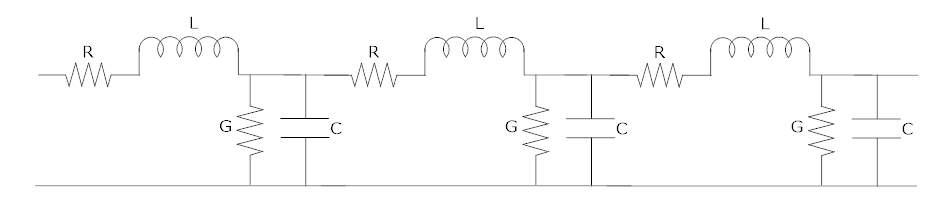
\includegraphics[width=1\linewidth]{./graphics/sixth}
\caption{Distributed elements for lossless transmission}
\end{figure}
In the diagram above, the resistance, capacitance, inductance and conductance are all per unit length values. We have defined the quantities which are called the PRIMARY CONSTANT of the transmission line which is;\\\\
Resistance per unit length – Ohms/metre\\
Inductance per unit length – Henry/metre\\
Capacitance per metre – Farad/metre\\
Conductance per metre – Siemens/metre\\

After the primary constants have been determined then the analysis of the transmission line can be carried out by;
\begin{enumerate}
\itemsep0em
\item Dividing the transmission line into small segments.
\item Writing down Kirchoff's law of voltage and current for the segment.
\item Carry out the analysis when the segment goes to zero to enable the analysis to be valid for any high frequency or any low wavelength. 
\item Apply voltage to the segment that causes current to flow into the circuit.
\end{enumerate}
\begin{figure}[h]
\centering
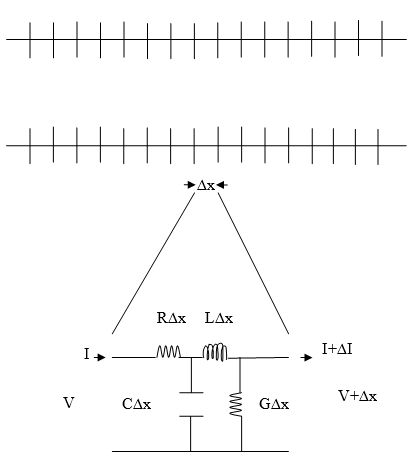
\includegraphics[scale=0.4]{./graphics/seventh}
\caption{circuit analysis of a small segment of the transmission line}
\end{figure}
Since the segment is very small and voltage has an angular frequency $ \omega $ then;
\begin{align}  
\Delta V = - (R \Delta x + j\omega L\Delta x)I
\label{eqn:voltage}
\end{align}
\begin{align}
\Delta I = - (G \Delta x + j \omega C \Delta x)V
\label{eqn:current}
\end{align}
We notice a negative sign in $ \Delta I $ and $ \Delta V $ expression which is because as we move in the direction of current flow there is a drop in voltage that will make (I +$  \Delta I $) and (v + $ \Delta V) $ values lesser than I and V at the start node.

For equations \ref{eqn:voltage} and \ref{eqn:current} to be valid at all frequencies, $ \Delta x $ must tend to zero.\\
From equation~\ref{eqn:voltage} we have;
\[ \Delta V = - (R \Delta x + j\omega L\Delta x)I \]
\[ \Delta V = - (R + j\omega L)\Delta x I \]

\[ \frac{	\Delta V }{\Delta x} = \frac{ - (R  + j\omega L)\Delta x I}{\Delta x} \]

\[ \frac{	\Delta V }{\Delta x} =  - (R  + j\omega L) I \]

\[ \lim_{ \Delta x\to 0} \frac{\Delta V}{ \Delta x} = \frac{ dV}{ \ dx} = - (R + j \omega L)I \]
 \begin{align}
\frac{ dV}{ \ dx} = - (R + j \omega L)I 
\label{eqn:deltav}
 \end{align} 
Also, from equation~\ref{eqn:current} we have,
\[ \Delta I = - (G \Delta x + j\omega C\Delta x)V \]
\[ \Delta I = - (G + j\omega C)\Delta x V \]

\[ \frac{	\Delta I }{\Delta x} = \frac{ - (G + j\omega C)\Delta x V}{\Delta x} \]
   
\[ \frac{	\Delta I }{\Delta x} =  - (G + j\omega C) V \]
   
\[ \lim_{ \Delta x\to 0}	\frac{ \Delta I}{ \Delta x} = \frac{dI}{dx} = - (G + j\omega C)V \]
\begin{align}
\frac{dI}{dx} = - (G + j\omega C)V 
\label{eqn:deltai}
\end{align}
Equations \ref{eqn:deltav} and \ref{eqn:deltai} are said to be \textbf{Coupled Equations} since $ \frac{dV}{dx} $ is related to $I$ and $ \frac{dI}{dx} $  is related to $V$.

Hence, we see that the voltage and current as $ \Delta x \rightarrow $ 0 are not related by algebraic equations but by a differential equation.\\
By differentiating equations \ref{eqn:deltav} and \ref{eqn:deltai} again, we have; 
\begin{align}
\frac{d^{2}V}{dx^{2}} = - (R + j\omega L)\frac{dI}{dx} 
\label{eqn:delta2v}
\end{align}
\begin{align}
\frac{d^{2}I}{dx^{2}} = - (G + j\omega C)\frac{dv}{dx}
\label{eqn:delta2i}
\end{align}
Substituting equation \ref{eqn:deltai} into \ref{eqn:delta2} we have,
\[ 	\frac{d^{2}V}{dx^{2}} = - (R + j\omega L)\times {- (G + j\omega C)V} \]
\begin{align}
 \frac{d^{2}V}{dx^{2}} = (R + j\omega L)(G + j\omega C)V 
\label{eqn:deqn}
\end{align}   
\\
The coefficient of V in equation~\ref{eqn:deqn} must be a primary quantity of the transmission line since it depends on the primary constant of the transmission line and the frequency of operation $ \omega$. Let's call the quantity $ \gamma^{2}. $ 

Therefore, 
\begin{align}
\frac{d^{2}V}{dx^{2}} = \gamma^{2}V 
\label{eqn:deqnv}
\end{align}
\begin{align}
\frac{d^{2}I}{dx^{2}} = \gamma^{2}I 
\label{eqn:deqni}
\end{align}
Equations \ref{eqn:deqnv} and \ref{eqn:deqni} are referred to as the \textbf{Telegraphers Equation}.

These are now the voltage and current expressions that governs a transmission line. The quantity $ \gamma $ is called the \textbf{Propagation Constant}. The quantity $V$ and $I$ are sinusoidal and so vary with $ e ^{j\omega t}$. The quantity $ e ^{j\omega t} $ helps take care of the harmonic time variation in V an I. \\
Since $ \gamma $ is a constant for a given line and frequency, 
\[ \frac{d^{2}V}{dx^{2}} = \gamma^{2}V\]\\
Therefore; 
\begin{align}
V(x) = V^{+} e ^{- \gamma x} + V^{-}e^{\gamma x}  
\label{eqn:solnv}
\end{align}
$ 	V(x) = V^{+} e ^{- \gamma x} + V^{-}e^{\gamma x} $  is the RMS or peak value. 

To find the instantaneous value of $V$, we multiply equation~\ref{eqn:solnv} by $ e ^{j\omega t}$.  V depends on $x$ and $t$. So,
\[ 	V(x,t) = V^{+} e^{-\gamma x}e^{j\omega t} + V^{-} e^{\gamma x}e^{j\omega t} \]
The only way to show the amplitude and the initial phase is through a complex number. therefore,

$ V^{+} $= Complex value of voltage at x= 0 location with a certain initial phase. Hence why V is always complex;

\[ 	V(x,t) = V^{+} e^{-\gamma x}e^{j\omega t} + V^{-} e^{\gamma x}e^{j\omega t} \]

But $ \gamma = \alpha + j\beta $	 is also a complex quantity. 
\[ V^{+}e^{- \gamma x}e^{j \omega t} = V^{+}e^{-( \alpha + j \beta )x}e^{j \omega t} = V^{+}e^{-\alpha x}e^{j(\omega t - \beta x)}
 \]

$ V^{+}e^{-\alpha x} $ is a voltage whose amplitude varies exponentially along the transmission line and the phase of the voltage is a combination of space and time from $  (\omega t- \beta x) $, $ \omega t $ from time and $ \beta x  $ from space. Hence $ V^{+}e^{-\gamma x}e^{jwt} \equiv V^{+}e^{-\alpha x}e^{j( \omega t-\beta x)} $ is the first point of V(x,t) and represent something whose amplitude varies along the length and the phase of which is a combination of space and time.\\

For understanding say, $  V^{+} $ is real and positive and $ \alpha= 0 $ then
\begin{align*}
V^{+}e^{-\alpha x}e^{j( \omega t-\beta x)} = V^{+} e^{j( \omega t-\beta x)}
\end{align*}
We plot this as a function of space and time
 \[ V^{+}e^{j( \omega t-\beta x)} = V^{+}cos(\omega t- \beta x) +  V^{+}jsin(\omega t- \beta x)\footnote{Recall from Euler's formula; $ e^{j\theta} = cos\theta + jsin\theta $}\]

Since we want real voltage we take only $ V^{+}cos(\omega t- \beta x) $ and plot variation of $ V $ with respect to $ x $ and $ t $. We have the graph shown below for different $ t $, as $ t $ increases, a point in the plot moves rightward. Hence with respect to space and time, the graph moves rightward as time increases. This is called a \textbf{Travelling wave phenomenon}.

\begin{figure}[h]
\centering
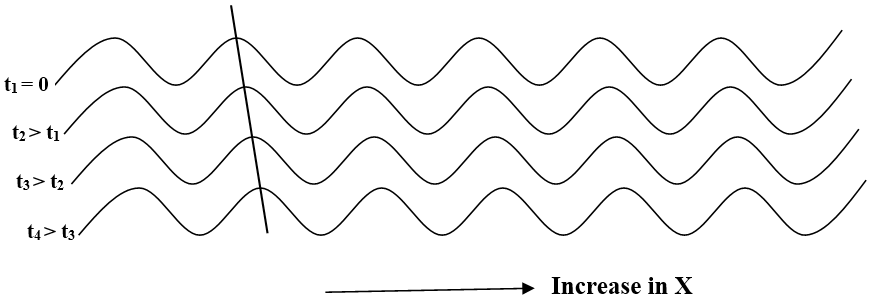
\includegraphics[width=1\linewidth]{./graphics/ABC}
\caption{Voltage as a function of X for different time}
\end{figure}
Hence  $ V^{+}e^{j(\omega t- \beta x )} $ is a positive or progressive travelling wave as it moves rightward with an increase in time. Similarly, when $ V^{-}e^{j( \omega t+ \beta x )} $ is plotted on the graph, the point starts moving leftward with an increase in time and it is called \textbf{negative travelling wave}.

\begin{figure}[h]
\centering
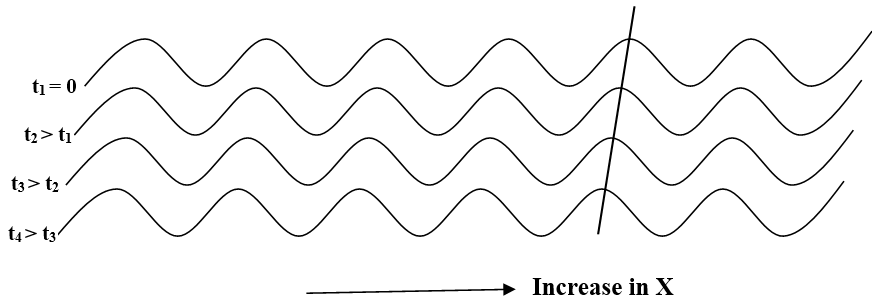
\includegraphics[width=1\linewidth]{./graphics/ABCD}
\caption{Voltage as a function of X for different time}
\end{figure}

Hence with high-frequency circuit analysis, the voltages and current have to be visualized in the form of waves. 

In conclusion, we see that a departure from the lumped element analysis to the distributed circuit analysis radically changes the approach to circuit analysis to a voltage and current that exist in the form of waves on the electrical circuits. 
%\chapter{The Propagation Constant}
In the previous chapter, we showed that voltage and current appear in form of waves on transmission lines and that the properties of this travelling wave are governed by the propagation constant, $\gamma$. In this chapter, we would try to understand the physical significance of this complex quantity $\gamma$ and also solve some problems to get a feel of the effect of propagation constant $\gamma$ on transmission lines.

\section{The complex quantity $\gamma$}We showed earlier that,

\begin{align*}
\gamma &= \sqrt{(R + \jmath\omega L)(G + \jmath\omega C)} \\
\gamma & = \alpha + \jmath\beta
\end{align*}
Where $R$ is the resistance per unit length\\

\hspace{13pt}$L$ is the inductance per unit length\\
  
\hspace{13pt}$C$ is the capacitance per unit length\\
  
\hspace{13pt}$G$ is the conductance per unit length\\ 
For the forward travelling wave, we had the expression
\begin{equation}
V^+e^{-\gamma x} =\left|  V^+\right| e^{-(\alpha + \jmath\beta)x}e^{\jmath\phi}
\end{equation}
If we assume $V^+$ to be real and have an initial phase $\phi = 0$, then;
\begin{equation*}
V^+e^{-\gamma x} = \left| V^+\right| e^{-(\alpha + \jmath\beta)x}e^{\jmath (0)}
\end{equation*}
But $ e^{j(0)} = e^0 = 1 $, the expression then simplifies to
\begin{equation}
V^+e^{-\gamma x} = \left| V^+\right| e^{-\alpha x}e^{-\jmath\beta x}
\label{eqn3.2}
\end{equation}
\section{The Phase constant}
From the Equation \ref{eqn3.2}, we see that as the wave propagates i.e as the value of x increases, the quantity $\mid V^+\mid e^{-\alpha x}$ is exponentially decreasing while $e^{-\jmath\beta x}$ is the sinusoidal part that oscillates because according to Euler's formula\footnote{
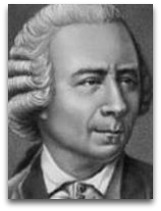
\includegraphics[scale=0.2]{./graphics/euler}

Named after Leonhard Euler (15 April 1707 - 18 September 1783). He was a Swiss mathematician, physicist, astronomer, logician and engineer who made important and influential discoveries in many branches of mathematics like infinitesimal calculus and graph theory. He was a friend of Daniel Bernoulli.
} 
$e^{-\jmath\beta x} = \cos{\beta x} - \jmath \sin{ \beta x}$. Hence phase (space phase) is obtained from $e^{-\jmath\beta x}$.\\

We now see that the equation 
\begin{equation}
\gamma = \alpha + \jmath\beta 
\end{equation}
has $\alpha$ that controls the amplitude of the wave as we move in the x-direction and $\beta$ controls the phase of the wave along the transmission line. Hence;
\begin{equation}
\text{Space phase} = -\jmath\beta
\end{equation}
As we travel in the positive x-direction, the phase lags more and this linearly varies with x for a given value of $\beta$. Hence $\beta$ represents the phase change per unit length.
\begin{equation}
\beta = \frac{\text{phase change}}{\text{unit length}} \quad\left(\frac{radian}{m}\right)
\end{equation}
We know that a phase change of 2$\pi$ corresponds to wavelength. From;
\begin{equation}
\phi = \beta x \quad and  \quad\phi = 2\pi
\end{equation}
\begin{align*}
2\pi = \beta\lambda \quad or \quad\beta = \frac{2\pi}{\lambda} \quad
\end{align*}
where, $ x = \lambda $ (distance\ travelled).\\

For most transmission line problems involving wave motion, $\lambda$ is not given, instead, $\gamma$ (propagation constant) is given in the complex form and $\beta$ is analyzed from the value of $\gamma$ given. The propagation constant $\gamma$ is then calculated from $\beta$.
Since $\gamma$ depends on the primary constants $R$, $L$, $G$ and $C$ at operating frequency $\omega$, we then conclude that the quantity $\beta$ called \textbf{Phase Constant} is also a function of frequency $\omega$. In other words, we conclude that the wavelength of waves on a transmission line is a function of the line parameter changes, phase constant change, and wavelength change.
\section{The Attenuation constant}
Recall that amplitude varies as $\lvert V^+ \rvert e^{-\alpha x}$ so that we have maximum amplitude at $x = 0$. As x increases, the amplitude decreases exponentially with $\alpha x$. 
\begin{figure}[h]
\centering
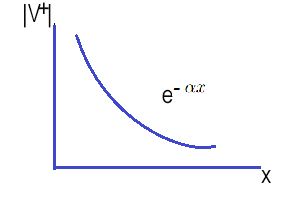
\includegraphics[scale = 0.45]{./graphics/VversusXcurve}
\caption{The amplitude versus distance plot}
\label{fig:VversusXcurve}
\end{figure}

From Figure~\ref{fig:VversusXcurve}, $\alpha$ is a parameter that measures how fast amplitude decay occurs in the transmission line wave. This quantity $\alpha$ is called the \textbf{Attenuation Constant}. The attenuation constant measures how the wave attenuates (reduces in its value) as it travels along the structure. So,
\begin{align*}
\text{Attenuation constant,}\ \alpha = \frac{Nepers}{meter}
\end{align*}

If $\alpha$ = 1(Nepers/meter)\footnote{
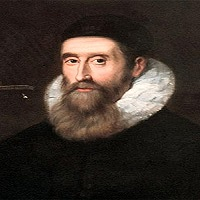
\includegraphics[scale=0.2]{./graphics/johnnapier2}

The unit's name is derived from the name of John Napier. John Napier of Merchiston (1550 – 4 April 1617); also signed as Neper, Nepair; nicknamed Marvellous Merchiston, was a Scottish landowner known as a mathematician, physicist, and astronomer. He is best known as the discoverer of logarithms, he also invented the so-called \textquotesingle\textquotesingle Napier's bones\textquotesingle\textquotesingle}, then the voltage value will reduce from its initial value to $\frac{1}{e}$ for a distance x = 1 meter. So $\alpha$ relates the distance over which the amplitude drops to $\frac{1}{e}$ of its initial value. This length at which we get $\frac{1}{e}$ is called the \textbf{Characteristic Length}. 

So, a distance $x = \frac{1}{\alpha}$ tells you the effective travel distance in the transmission line beyond which the amplitude drops below $\frac{1}{e}$ of its initial value. Since the wave is reducing to $\frac{1}{e}$ of its initial value, the power of the wave also reduces. Taking the ratio of the initial amplitude and final amplitude after the effective travel distance we have;
\begin{align*}
 \frac{\lvert V^+\rvert}{\lvert V^+\rvert e ^{-\alpha x}} \quad \text{because the initial amplitude at } x = 0
\end{align*}
\begin{align*}
\text{with }x = \frac{1}{\alpha},\text{ the expression reduces to }\frac{1}{e}
\end{align*}
We would now proceed to express the attenuation constant in decibels per metre ($\frac{dB}{meter}$), as this is the unit in which the attenuation constant is given in most data sheets.
\begin{align*}
dB = -20\log_{10}(\frac{1}{e^{\alpha x}})
\end{align*}
$ dB = -20\log_{10}(e^{-\alpha x}), \ with \ \alpha = 1 $ Neper/meter,\\ and $ x = 1m $. \\
$ dB = -20\log_{10}(e^{-1}) = 8.68\ dB/m  $\\
Therefore, 1 Neper/m = 8.68 dB/m.\\

As in propagation constant $\gamma$, the attenuation constant $\alpha$ depends on the primary constant of the transmission line as well as the frequency of operation $\omega$. In general, the propagation constant $\gamma$ which is a combination of phase constant $\beta$ and attenuation constant $\alpha$ is a function of primary line parameters and frequency of operation. Hence as $\omega$ increases, $\alpha$ increases. This is the reason some structures which were satisfactorily good conductors, at low frequencies become bad conductors at high frequencies (i.e the conductor becomes a more lossy line at high frequencies).

\begin{exmp}
Let R = 0.5 $\Omega$ /m, L = 0.2$\mu$H /m, C = 100pF/m, G = 0.1 $\Omega$ /m, freq = 1GHz. \ Calculate\ the\ propagation\ constant,\ attenuation\ constant\ and\ phase\ constant\ for\ this\ line. \\\\\\\\\\

$\textbf{Solution.}$\\\\
$ \gamma = \sqrt{(R+\jmath\omega L)(G + \jmath\omega C)}$\\\\
But,$ \ \omega = 2\pi f\quad$ and $\quad f = 1GHz = 1 \times 10^9 $ Hz\\\\
$ \omega = 2\pi \times 10^9 $ rad/s.\\\\
Substituting into the $ \gamma $ expression; \\\\
$\sqrt{[0.5+\jmath (2\pi \times 10^9)\times 0.2 \times 10^{-6}][0.1 + \jmath(2\pi \times 10^9) \times 100 \times10^{-12}]}  $\\\\
$ \gamma = \sqrt{(0.5 + \jmath 400\pi)(0.1 + \jmath 0.2\pi)} $\\\\
Expanding,\\\\
$ = \sqrt{0.5(0.1) + 0.5(\jmath 0.2\pi) + \jmath 400\pi(0.1) + \jmath 400\pi(\jmath 0.2\pi)} $ \\\\
Recall  that,$ \quad \jmath \times \jmath = \sqrt{-1} \times \sqrt{-1} = (\sqrt{-1})^2 = -1 $\\\\
$ =\sqrt{0.05 + \jmath 0.31416 +\jmath 125.6637 - 789.568} $ \\\\
$ = \sqrt{-789.518 + \jmath 125.97786} $ \\

We are now faced with the challenge of finding the square root of a complex number.
\footnotetext[3]{
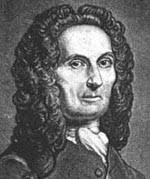
\includegraphics[scale=0.3]{./graphics/demoivre}

Named after Abraham de Moivre (26 May 1667 – 27 November 1754). He was a French mathematician known for de Moivre's formula, a formula that links complex numbers and trigonometry, and for his work on the normal distribution and probability theory. He was a friend of Isaac Newton, Edmond Halley, and James Stirling.}\\
To find the square root, we apply DeMoivre's theorem \footnotemark[3]. It states; $ \quad Z^{\frac{1}{n}} = |Z|^{\frac{1}{n}}\angle\frac{\theta}{n} $\\\\
We first convert the complex number to polar form.\\\\
-$ 789.518 + \jmath 125.9778 = 799.5055\angle 170.934\textdegree $\\\\
$ \sqrt{-789.518 + \jmath 125.9778} = \sqrt{799.5055}\angle \frac{170.934}{2} $\\\\
$ =28.2\angle 85.467 $\\\\
Converting back to cartesian form; \\\\
Propagation constant,$\quad\gamma=2.23 +\jmath 28.1 $\\\\
From the expression; \\
$ \alpha = 2.23467 $ Nepers/m, $ \beta = 28.1871 $ rad/m\\\\
We now convert the attenuation constant to dB/m; \\
1 Nepers/m = 8.68dB/m \\\\
2.23467 Nepers/m = 19.3969 dB/m

\end{exmp} 

\begin{exmp}
From previous example, say at x = 0, t = 0, V = 8.66V. Find the voltage at x = 1 and t = 100ns at point B on the transmission line. Also, find the peak voltage at x = 1m. Assume the wave travels from left to right, and the initial phase $\phi = 30^o$.\\
If the wave travels from right to left, find the voltage at B.
\begin{figure}[h]
\centering
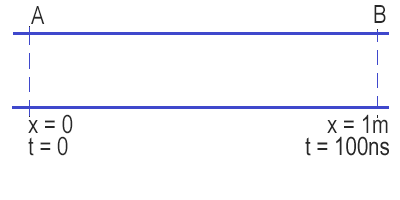
\includegraphics[width=1\linewidth]{./graphics/TL}
\caption{The transmission line showing points A and B.}
\end{figure}

\textbf{Solution.} \\ 
At x = 1, the voltage is maximum, at x = 0 i.e A, V = 8.66v. Due to the direction of wave travel, we expect its amplitude to reduce to a smaller value at B. The expression
\begin{align}
V(x,t) = Re{[\left| V^+\right|  e^{-\alpha x}.e^{-\jmath\beta x + \jmath\omega t}.e^{+\jmath\phi}]} 
\label{eqn:voltagesoln}
\end{align}
represents the forward travelling or progressive wave moving along the +x direction.\\
Extracting the real part and including the initial phase.
\begin{align*}
V(x,t) = \lvert V^+\rvert cos(\phi + \omega t - \beta x)e^{-\alpha x}
\end{align*}
\begin{figure}[h]
\centering
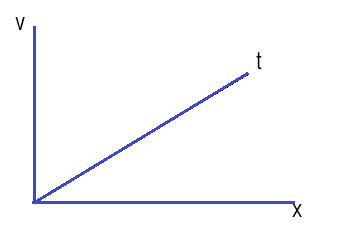
\includegraphics[scale=0.5]{./graphics/VversusX}
\caption{Voltage versus distance with time}
\end{figure}

$\lvert V^+\rvert e^{-\alpha x} $ gives the amplitude variation with distance $ x $. \\
$ \phi + \omega t - \beta x $ gives the phase (including the initial phase $ \phi $ ).\\

Substituting x = 0, t = 0, and $\phi = 30^o$ into equation~\ref{eqn:voltagesoln},
\begin{align*}
V(x,t) = V(0,0) &= 8.66v \\
V(x,t) &= \lvert V^+\rvert cos(\phi + \omega (0) - \beta (0)e^{-\alpha (0)}\\
8.66 &= \lvert V^+\rvert cos(\phi)\\
8.66 &= \lvert V^+\rvert cos(30)\\
\lvert V^+\rvert &= 10v
\end{align*}
Substituting x = 1m, t = 100ns, and $\phi = 30^o$ into equation~\ref{eqn:voltagesoln},\\\\
$ V(x,t) = 10 cos(\frac{\pi}{6} + 2\pi \times 10^9\times 100\times 10^{-9} - 28.18\times 1)e^{-2.235\times 1} $\\\\
$ = 10 \times -0.815 \times e^{-2.235} $\\\\
$ = -0.872v $\\
To find the peak voltage at x = 1,
\begin{align*}
V(1,t) = 10cos(\frac{\pi}{6} + 2\pi \times 10^9t - 28.18)e^{-2.235}
\end{align*}
but the value is maximum when $cos(\frac{\pi}{6} + 2\pi \times 10^9t - 28.18) = 1$, 
\begin{align*}
V_{max} &= 10e^{-2.235}\\
V_{max} &= 1.07v
\end{align*}
We observe from the solution that attenuation took place since the amplitude reduced from 8.66v to -0.88v.\\ \\
If the wave travels from right to left
\begin{align*}
\hspace{-0.25in}V(x,t) &= Re{[V^+ e^{+\alpha x}.e^{+\jmath\beta x + \jmath\omega t}e^{+\jmath\phi}]}\\
&= \lvert V^+\rvert cos(\phi + \omega t + \beta x)e^{+\alpha x}\\
&= 10 cos(\frac{\pi}{6} + 2\pi \times 10^9\times 100\times 10^{-9} + 28.18\times 1)e^{+2.235\times 1}\\
&= 10 \times -0.9093 \times e^{+2.235}\\
&= -84.99v
\end{align*} 	
\end{exmp}

\section{The Characteristic Impedance}
Recall from the original differential equation;
\begin{align*}
\frac{dV}{dx} = -(R+\jmath\omega L)I \quad and\quad \frac{dI}{dx} = -(G+\jmath\omega C)V
\end{align*}
Also, 
\begin{align*}
V = V^+e^{-\gamma x}+V^-e^{+\gamma x}\quad and \quad I = I^+e^{-\gamma x}+I^-e^{+\gamma x}
\end{align*}
Substituting $V$ and $I$ into the differential equation,
\begin{align*}
\frac{d}{dx}(V^+e^{-\gamma x}+V^-e^{+\gamma x}) &= -(R+\jmath\omega L)(I^+e^{-\gamma x}+I^-e^{+\gamma x})\\
-\gamma V^+e^{-\gamma x}+\gamma V^-e^{+\gamma x} &= -(R+\jmath\omega L)(I^+e^{-\gamma x}+I^-e^{+\gamma x})
\end{align*}
 $(V^+,I^+)$ represent forward traveling waves, while $(V^-,I^-)$ represent backward traveling waves for voltage and current respectively. The relationship between voltage and current has to be satisfied at every point along the transmission line. This will happen if and only if
\begin{align*}
-\gamma V^+e^{-\gamma x} &= -(R+\jmath\omega L)I^+e^{-\gamma x}\quad and\quad \frac{V^+}{I^+} = \frac{R+\jmath\omega L}{\gamma}\\
Also,    \ \ \ \ \                &\\
\gamma V^-e^{+\gamma x} &= -(R+\jmath\omega L)I^-e^{+\gamma x}\quad and\quad \frac{V^-}{I^-} = -\frac{R+\jmath\omega L}{\gamma}
\end{align*}
The expressions above show the relationship between forward and backward travelling waves for voltage and current.\\ \\
Recall that $\gamma = \sqrt{(R + \jmath\omega L)(G + \jmath\omega C)}$, therefore
\begin{align*}
\frac{V^+}{I^+} = \frac{R+\jmath\omega L}{\sqrt{(R + \jmath\omega L)(G + \jmath\omega C)}}
\end{align*}
We can play around with this expression as follows,
\begin{align*}
\frac{V^+}{I^+} &= \frac{\sqrt{(R+\jmath\omega L)^2}}{\sqrt{(R + \jmath\omega L)(G + \jmath\omega C)}}\\
&=\sqrt{\frac{(R+\jmath\omega L)(R+\jmath\omega L)}{(R + \jmath\omega L)(G + \jmath\omega C)}}\\
\frac{V^+}{I^+} &=\sqrt{\frac{R+\jmath\omega L}{G+\jmath\omega C}}
\end{align*}
similarly,
\begin{align*}
\frac{V^-}{I^-} = \frac{-(R+\jmath\omega L)}{\sqrt{(R + \jmath\omega L)(G + \jmath\omega C)}}
\end{align*}
\begin{align*}
\frac{V^-}{I^-} &= \frac{-\sqrt{(R+\jmath\omega L)^2}}{\sqrt{(R + \jmath\omega L)(G + \jmath\omega C)}}\\
&=-\sqrt{\frac{(R+\jmath\omega L)(R+\jmath\omega L)}{(R + \jmath\omega L)(G + \jmath\omega C)}}\\
\frac{V^-}{I^-} &=-\sqrt{\frac{R+\jmath\omega L}{G+\jmath\omega C}}
\end{align*}

$\sqrt{\frac{R+\jmath\omega L}{G+\jmath\omega C}}$ is another characteristic of the transmission line since it depends only on the primary constants and the frequency of operation. Also, this parameter is the ratio of voltage and current and as such has a definition of impedance. Hence the reason is called the \textbf{Characteristic Impedance} of the line and it is denoted by $Z_o$.
\begin{equation}
Z_o = \sqrt{\frac{R+\jmath\omega L}{G+\jmath\omega C}}
\end{equation}
Later you would see that $Z_o$ governs energy flow on the transmission line. So these two parameters, the propagation constant $\gamma$ and the characteristic impedance $Z_o$ completely characterize the propagation of wave along a transmission line. Though R, L, G and C are primary parameters, they are hardly given in any transmission line problem. 

Most of the time transmission line is characterized by its propagation constant $\gamma$ and characteristic impedance $Z_o$. They are usually given in the datasheet of transmission lines and this is sufficient information to solve any transmission line problem.
From the derivation of characteristic impedance, we can write
\begin{equation}
\frac{V^+}{I^+} = Z_o\quad and\quad \frac{V^-}{I^-} = -Z_o
\end{equation}
It is clear that at any point on the transmission line, the ratio of voltage to current (forward or backward) is always constant i.e equal to characteristic impedance.\\

Hence a forward travelling wave sees an impedance of $Z_o$ and the reverse travelling wave sees an impedance of $-Z_o$. If $Z_o$ is real, it means the forward travelling wave sees a positive resistance while the backward travelling wave sees a negative resistance.

\textbf{But what does a negative resistance mean?}
Ordinarily, energy flow is from the generator to the load which the positive resistance represents. The negative resistance means energy is being carried backwards i.e energy is flowing from the load into the generator.\\

In conclusion, irrespective of the boundary condition of the transmission line, the forward travelling wave always sees an impedance equal to the characteristic impedance while a backward travelling wave sees a negative of the characteristic impedance.\\

We established that;
\begin{align*}
\frac{V^+}{I^+} = Z_o,\quad I^+ = \frac{V^+}{Z_o}
\end{align*}
\begin{align*}
\frac{V^-}{I^-} = -Z_o,\quad I^- = -\frac{V^-}{Z_o}
\end{align*}
We can now rewrite the expressions for voltage and current as
\begin{equation}
V = V^+e^{-\gamma x}+V^-e^{+\gamma x}
\label{eqn:voltage}
\end{equation}
\begin{equation}
I = \frac{V^+}{Z_o}e^{-\gamma x}-\frac{V^-}{Z_o}e^{+\gamma x}
\label{eqn:current}
\end{equation}

\section{Defining boundary condition}
\begin{figure}[h]
\centering
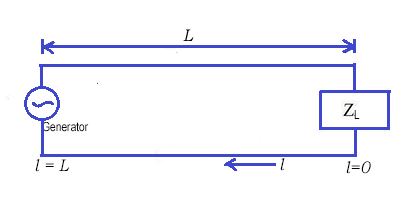
\includegraphics[scale=0.45]{./graphics/tlcircuit}
\caption{The transmission line showing generator and load}
\end{figure}
Up until now, we have not defined the boundary condition of the transmission line. So let's do that here. We have two spatial locations on the transmission line, one at the generator and the other where an arbitrary load $Z_L$ is connected. To define boundary conditions, we define the spatial distance from the load end, the origin, so that all distances move from the load end towards the generator. So we now have a parameter that moves towards the generator from the load side. At the load point $l = 0$ and at the generator, $l = L$. So $l = -x$ is in our transmission line equation. Substituting $l = -x$ in Equations \ref{eqn:voltage} and \ref{eqn:current}, we have
\begin{equation}
V = V^+e^{+\gamma l}+V^-e^{-\gamma l}
\label{eqn:voltagefromload}
\end{equation}
\begin{equation}
I = \frac{V^+}{Z_o}e^{+\gamma l}-\frac{V^-}{Z_o}e^{-\gamma l}
\label{eqn:currentfromload}
\end{equation}
$l = 0$ corresponds to the load location or the receiving end of the transmission line and $l = L$ is the generator point or transmitting end of the transmission line.

\section{The reflection coefficient}
At $l = 0$, $Z = Z_L$ since $Z_L$ terminates the transmission line at this point. Substituting $l = 0$ into Equations (3.12) and (3.13),
\begin{align*}
V &= V^+e^{+\gamma (0)}+V^-e^{-\gamma (0)} = V^+ + V^-\\
I &= \frac{V^+}{Z_o}e^{+\gamma (0)}-\frac{V^-}{Z_o}e^{-\gamma (0)} = \frac{V^+}{Z_o} - \frac{V^-}{Z_o} \\
I &= \frac{V^+ - V^-}{Z_o}
\end{align*}
\begin{align*}
\frac{V}{I} = \left( \frac{V^+ + V^-}{1}\right)  \times \left( \frac{Z_o}{V^+ - V^-}\right) 
\end{align*}

\begin{equation*}
Z_{L} = \frac{V}{I}\left|_{l = 0} = Z_{o} \left[ \frac{V^+ + V^-}{V^+ - V^-} \right]\right.    
\end{equation*}

\begin{equation}
Z_L = Z_o \left[ \frac{V^+ + V^-}{V^+ - V^-} \right]
\end{equation}
It is clear from the expression above that the load impedance is related to the characteristic impedance and also related to the amplitude of the forward and backward waves. 
\begin{equation*}
Dividing\ top\ and\ bottom\ by\ V^+,\quad
Z_L = Z_o\left[ \frac{\frac{V^+ + V^-}{V^+}}{\frac{V^+ - V^-}{V^+}}\right] 
\end{equation*}
\begin{equation}
Z_L = Z_o\left[ \frac{1+ \frac{V^-}{V^+}}{1 - \frac{V^-}{V^+}}\right] 
\label{eqn:impedatload}
\end{equation}
Here we see that the absolute values of $V^+$ and $V^-$ do not matter, instead, the ratio $\frac{V^-}{V^+}$ is what's important. Hence we define a new parameter on which $Z_L$ depends. This parameter is known as the reflection coefficient.\\ \textbf{Reflection Coefficient} can be defined as the ratio of backward travelling wave to forward travelling wave on the transmission line.
The reflection coefficient is denoted by \footnote[3]{$\Gamma$ is capital Gamma, the third letter of the Greek alphabet.}$\Gamma$.
\begin{equation*}
\Gamma = \frac{\text{backward travelling wave}}{\text{forward travelling wave}}
\end{equation*}
\begin{equation}
\Gamma (l) = \frac{V^-e^{-\gamma l}}{V^+e^{+\gamma l}}
\label{eqn:rfc}
\end{equation}
 $\Gamma(l)$ is the reflection coefficient at any point on the line.\\ \\
At $l = 0$,
\begin{equation*}
\Gamma (0) = \frac{V^-e^{-\gamma (0)}}{V^+e^{+\gamma (0)}}
\end{equation*}
\begin{equation}
\Gamma (0) = \Gamma_L = \frac{V^-}{V^+}
\label{eqn:rfcatload}
\end{equation}
$\Gamma_L$ is the reflection coefficient at the load point on the line. From now henceforth, $\Gamma_L$ will be used to represent the reflection coefficient at the load point.\\
 Substituting Equation~\ref{eqn:rfcatload} into Equation~\ref{eqn:rfc},
\begin{equation*}
\Gamma (l) = \Gamma_L\frac{e^{-\gamma l}}{e^{+\gamma l}}
\end{equation*}
\begin{equation}
\Gamma (l) = \Gamma_L e^{-2\gamma l}
\end{equation}
Recall, Equation~\ref{eqn:impedatload} was derived at the load point. We would now derive the relationship at any point on the line. \\ \\
Dividing Equation~\ref{eqn:voltagefromload} by Equation~\ref{eqn:currentfromload},

\begin{align*}
\frac{V}{I} = \frac{V^+e^{+\gamma l}+V^-e^{-\gamma l}}{1}\times \frac{Z_o}{V^+e^{+\gamma l}-V^-e^{-\gamma l}}
\end{align*}
\begin{align*}
= Z_o\left( \frac{V^+e^{+\gamma l}+V^-e^{-\gamma l}}{V^+e^{+\gamma l}-V^-e^{-\gamma l}}\right) 
\end{align*}
\begin{align*}
\text{Dividing top and bottom by }V^+e^{+\gamma l}
\end{align*}
\begin{align*}
= Z_o\left( \frac{\frac{V^+e^{+\gamma l}}{V^+e^{+\gamma l}}+\frac{V^-e^{-\gamma l}}{V^+e^{+\gamma l}}}{\frac{V^+e^{+\gamma l}}{V^+e^{+\gamma l}}-\frac{V^-e^{-\gamma l}}{V^+e^{+\gamma l}}}\right) 
\end{align*}
From Equation~\ref{eqn:rfc},
\begin{align*}
=Z_o\left( \frac{1+\Gamma (l)}{1 -\Gamma (l)}\right) 
\end{align*}
Substituting for $\Gamma (l)$ from Equation(3.18), we have the expression at any point on the line.
\begin{equation}
Z(l) = Z_o\left[ \frac{1 + \Gamma_L e^{-2\gamma l}}{1 - \Gamma_L e^{-2\gamma l}}\right] 
\end{equation}
At $l = 0$ 
\begin{align*}
Z_L = Z_o\left[ \frac{1 + \Gamma_L e^{-2\gamma (0)}}{1 - \Gamma_L e^{-2\gamma (0)}}\right] 
\end{align*}
\begin{equation}
Z_L = Z_o\left[\frac{1 + \Gamma_L}{1 - \Gamma_L}\right] 
\end{equation}
\begin{align*}
Z_L(1 - \Gamma_L) &= Z_o(1 + \Gamma_L)\\
Z_L - Z_o &= (Z_o + Z_L)\Gamma_L
\end{align*}
\begin{equation}
\Gamma_L = \frac{Z_L - Z_o}{Z_L + Z_o}
\end{equation}
The reflection coefficient tells you the ratio between reflected and incident voltage. It's a measure of how much energy is reflected from the transmission line.

Our intention is always to deliver maximum energy to the load, we, therefore, want the reflection coefficient to be as small as possible. So we shall find the condition to deliver maximum power to the load i.e no reflection on the transmission line.
%\chapter{Lossless and Low-Loss Transmission Line}\label{lec:lec4}
From the previous chapter, we have established that
\begin{align*}
\Gamma_L \equiv \Gamma{(0)} = \frac{Z_L - Z_0}{Z_L + Z_0}
\end{align*}
Where $\Gamma_L$ is the reflection coefficient at the load end when $l = 0$. $\Gamma_L$ \emph{is a measure of how much energy is reflected from the load end and is related to the terminating impedance of the line and the characteristics impedance}.

\section{Matched Condition of the transmission line}
The equation can be further expressed as
\begin{align*}
\Gamma_L = \frac{Z_L - Z_0}{Z_L + Z_0} =  \frac{V^-}{V^+}
\end{align*}

It can be observed that when  $Z_L = Z_0$, then there is no reflection from the load and hence maximum power is delivered to the generator.
\begin{align*}
\Gamma_L = \frac{V^-}{V^+} = 0\ (\text{when }Z_L = Z_0.) 
\end{align*}
Although $Z_0$ cannot be located on the transmission line, it does govern power flow in the transmission line. This condition that $Z_L = Z_0$ is called the \textbf{Matched condition}\index{matched condition} of the transmission line. The terminating impedance of the line is matched to the characteristic impedance. This condition is similar to the maximum power transfer theorem in a circuit, where if the load impedance is equal to the conjugate of the generator impedance, maximum power is transferred from the generator to the load. 
\begin{align*}
Z_L = Z_0 \quad (\text{Matched Load Condition})
\end{align*}
As the wave moves along the line, it sees $Z_0$. At $Z_L$, it suddenly sees an impedance discontinuity from $Z_0$ to $Z_L$ which is like a steep change because of that part of the energy that tends to get reflected by the generator on the transmission line. So, for maximum power transfer, the terminating load impedance must be equal to the characteristics impedance otherwise, maximum power transfer will not take place and there will always be reflection.

The reflection co-efficient at any point on the transmission line is given as:
\begin{align*}
\Gamma{(l)} = \frac{V^-e^{-\gamma l}}{V^+e^{\gamma l}} = \frac{\text{Backward wave}}{\text{Forward wave}}
\end{align*}
Therefore we can define the voltage and current at any point on the transmission line with respect to reflection coefficient $\Gamma(l)$.
\begin{equation}
V(l) = V^+e^{\gamma l} + V^-e^{-\gamma l}\label{eqn:voltagefromloadchp4}
\end{equation}
\begin{equation}
I(l) =\frac{V^+}{Z_0} e^{\gamma l} - \frac{V^-}{Z_0}e^{-\gamma l}\label{eqn:currentfromloadchp4}
\end{equation}
Dividing Equation~\ref{eqn:voltagefromloadchp4} by $V^+e^{\gamma l}$
\begin{align*}
\frac{V(l)}{ V^+e^{\gamma l}} = 1 + \frac{ V^-e^{-\gamma l}}{ V^+e^{\gamma l}}
\end{align*}
\begin{align*}
\frac{V(l)}{ V^+e^{\gamma l}} = 1 + \Gamma(l)
\end{align*}
We then cross-multiply to have
\begin{align*}
V(l) = V^+e^{\gamma l} (1 + \Gamma(l))
\end{align*}
The above equation gives the voltage at any point on the line.

Divide Equation~\ref{eqn:currentfromloadchp4} by $\frac{V^+}{Z_0} e^{\gamma l}$
\begin{dmath*}
\frac{I}{\frac{V^+}{Z_0} e^{\gamma l}} = 1 - \frac{\frac{V^-}{Z_0} e^{-\gamma l}}{\frac{V^+}{Z_0} e^{\gamma l}}
= 1 - \frac{V^-e^{-\gamma l}}{V^+e^{\gamma l}}
= 1 - \Gamma(l)
\end{dmath*}
We cross-multiply again to get,
\begin{align*}
I(l) = \frac{V^+}{Z_0} e^{\gamma l} (1 - \Gamma(l))
\end{align*}
Where $Z(l) = \frac{V(l)}{I(l)}$, we have
\begin{align*}
Z(l) = \frac{V(l)}{I(l)} = \frac{V^+e^{\gamma l} (1 + \Gamma(l))}{ \frac{V^+}{Z_0} e^{\gamma l} (1 - \Gamma(l))}
\end{align*}
$V^+ e^{\gamma l}$ cancels out to give,
\begin{align}
Z(l) = Z_0\left[\frac{1 + \Gamma(l)}{1 - \Gamma(l)}\right]
\end{align}
$Z(l)$ \emph{is the impedance measured at any location of the transmission line. It is related to the reflection coefficient at any point and the characteristic impedance}. $\Gamma(l)$ is the reflection coefficient at any point on the transmission line. Hence $Z(l)$ and $\Gamma(l)$ have a one-to-one relationship at any point along the transmission line.

\section{Impedance Transform Relationship}
Recall,
\begin{dmath*}
Z(l) = \frac{V(l)}{I(l)}
= \frac{V^+e^{\gamma l} + V^-e^{-\gamma l}}{\frac{V^+}{Z_0}e^{\gamma l} - \frac{V^-}{Z_0}e^{-\gamma l}}
= Z_0\left[\frac{V^+e^{\gamma l} + V^-e^{-\gamma l}}{V^+e^{\gamma l} - V^-e^{-\gamma l}}\right]
\end{dmath*}
Dividing  the numerator and denominator by $V^+e^{\gamma l}$ 
\begin{align*}
Z(l) = Z_0\left[\frac{1 + \frac{V^-e^{-\gamma l}}{V^+e^{\gamma l}}}{1 - \frac{V^-e^{-\gamma }}{V^+e^{\gamma }}}\right]
\end{align*}
Where $\Gamma_L = \frac{V^-}{V^+}$ and $\frac{e^{-\gamma l}}{e^{\gamma l}} = e^{-2\gamma l}$
\begin{align}
Z(l)=  Z_0\left[\frac{1 + \Gamma_L e^{-2\gamma l}}{1 - \Gamma_L e^{-2\gamma l}}\right]
\end{align}
But $\Gamma_L
= \frac{Z_L - Z_0}{Z_L + Z_0}$,
\begin{align*}
Z(l) = Z_0 \left[\frac{1 + (\frac{Z_L - Z_0}{Z_L + Z_0})e^{-2\gamma l}}{1 - (\frac{Z_L - Z_0}{Z_L + Z_0})e^{-2\gamma l}}\right]
\end{align*}
Multiplying the numerator and denominator by $Z_L + Z_0 $ gives
\begin{dmath*}
Z(l) = Z_0 \left[\frac{(Z_L + Z_0) + (Z_L - Z_0)e^{-2\gamma l}}{(Z_L + Z_0) - (Z_L - Z_0)e^{-2\gamma l}}\right]
= Z_0 \frac{e^{-\gamma l}}{e^{-\gamma l}}\left[\frac{(Z_L + Z_0)e^{\gamma l} + (Z_L - Z_0)e^{-\gamma l}}{(Z_L + Z_0)e^{\gamma l} - (Z_L - Z_0)e^{-\gamma l}}\right]
= Z_0 \left[\frac{Z_L e^{\gamma l} + Z_0e^{\gamma l} + Z_L e^{-\gamma l} - Z_0e^{-\gamma l}}{Z_L e^{\gamma l} + Z_0e^{\gamma l} - Z_L e^{-\gamma l} + Z_0e^{-\gamma l}}\right]
\end{dmath*}

Collect like terms
\begin{align*}
Z(l) = Z_0 \left[\frac{Z_L(e^{\gamma l} + e^{-\gamma l}) + Z_0(e^{\gamma l} - e^{-\gamma l})}{Z_L (e^{\gamma l} - e^{-\gamma l}) + Z_0(e^{\gamma l} + e^{-\gamma l})}\right]
\end{align*}
Before we proceed let us recall that 
\begin{align*}
\cosh(\gamma l) = \frac{e^{\gamma l} + e^{-\gamma l}}{2}\\
2\cosh(\gamma l) = e^{\gamma l} + e^{\gamma l}
\end{align*}
 and
\begin{align*}
\sinh(\gamma l) = \frac{e^{\gamma l} - e^{-\gamma l}}{2}\\
2\sinh(\gamma l) = e^{\gamma l} - e^{-\gamma l}
\end{align*}
Therefore,
\begin{dmath}
Z(l) = Z_0\left[\frac{2(Z_L\cosh(\gamma l) + Z_0\sinh(\gamma l))}{2(Z_L\sinh(\gamma l) + Z_0\cosh(\gamma l))}\right]
= Z_0\left[\frac{Z_L\cosh(\gamma l) + Z_0\sinh(\gamma l)}{Z_L\sinh(\gamma l) + Z_0\cosh(\gamma l)}\right]
\label{eqn:imp}
\end{dmath}

Equation~\ref{eqn:imp} shows that the impedance at any point $l$ is related to the load impedance $Z_L$ and the characteristics impedance $Z_0$. This enables us to move $Z_L$ to any point along the transmission line. Hence at $l = 0$, we have $Z_L$ but at $l = L$, the input impedance measured at the generator end will not be $Z_L$. It will depend on $Z_L$ and also the length of the line. So, if the length of the line keeps varying, the impedance you measure at the input end of the line will keep varying. 

Hence, if we design a circuit at high frequency and connect a load to the end, depending on the length of the transmission line, the input impedance will keep varying with length. From a circuit perspective, the input impedance is very important, so at high frequencies, the length connecting the load to the circuit matters as the input impedance seen by the generator varies with length.

From Equation~\ref{eqn:imp}:
\begin{align*}
Z(l) = Z_0\left[\frac{Z_L\cosh(\gamma l) + Z_0\sinh(\gamma l)}{Z_L\sinh(\gamma l) + Z_0\cosh(\gamma l)}\right]
\end{align*}
Now normalized with respect to $Z_0$ such that if,
$\frac{Z(l)}{Z_0} = \bar{Z}(l)$ and $\frac{Z_L}{Z_0} =\bar{Z}_L$ that is, normalized values.

Therefore, dividing both sides by $Z_0$
\begin{align*}
\frac{Z(l)}{Z_0} = \frac{Z_0}{Z_0}[\frac{Z_L\cosh(\gamma l) + Z_0\sinh(\gamma l)}{Z_L\sinh(\gamma l) + Z_0\cosh(\gamma l)}] 
\end{align*}
Dividing the numerator and denominator by $Z_0$
\begin{dmath}
\bar{Z}(l) =\left[ \frac{\frac{Z_L}{Z_0}\cosh(\gamma l) + \frac{Z_0}{Z_0}\sinh(\gamma l)}{\frac{Z_L}{Z_0}\sinh(\gamma l) + \frac{Z_0}{Z_0}\cosh(\gamma l)}\right]
= \frac{\frac{Z_L}{Z_0}\cosh(\gamma l) + \sinh(\gamma l)}{\frac{Z_L}{Z_0}\sinh(\gamma l) + \cosh(\gamma l)}
= \frac{\bar{Z}_L\cosh(\gamma l) + \sinh(\gamma l)}{\bar{Z}_L\sinh(\gamma l) + \cosh(\gamma l)}\ \text{(normalized impedance)}
\end{dmath}
That is, $\bar{Z} = \frac{Z}{Z_0}$.

Once again we see that on transmission line calculation, the absolute impedance does not mean anything; Rather it is the normalized impedance that matters most. Hence, $Z_0 = 50\Omega$ and $Z_L = 100\Omega$ gives same reflection as $Z_0 = 300\Omega$ and $Z_L =600\Omega$. Hence the reason why before starting any transmission line calculation, we ask ourselves what the characteristic impedance is, every impedance we have is then normalized to the characteristic impedance. So every calculation done in the transmission line is always done with respect to normalized impedances.

We then see that characteristic impedance which is not located anywhere or seen anywhere is always governing the energy flow of the transmission line.

Now if $\bar{Z}_L = 1$, then 
\begin{dmath*}
\bar{Z}(l) = {\frac{\bar{Z}_L\cosh(\gamma l) + \sinh(\gamma l)}{\bar{Z}_L\sinh(\gamma l) + \cosh(\gamma l)}} = 1
\end{dmath*}
Recall,
\[\frac{Z(l)}{Z_0} = \bar{Z}(l)\text{ and }\frac{Z_L}{Z_0} = \bar{Z}_L\]
So,
\[\frac{Z(l)}{Z_0} = 1\text{ and }\frac{Z_L}{Z_0} = 1
\]
means the impedance at every point equal to $Z_0$, if $Z_L = Z_0$ therefore $Z(l) = Z_0$. So, in this matched condition, the impedance $Z(l)$ measured at any point no longer depend on the length of the line. If a line is terminated by its characteristic impedance, there is no need to factor in the length of the line as every point along the line has an impedance equal to the characteristic impedance and this takes away all the worry about the line length.

The relationship of impedance transform will help us give a proper definition of characteristics impedance $Z_0$ which we know was related to the primary constants of the transmission line.

\section{Characteristic Impedance}  
Characteristic Impedance\index{characteristic impedance} \emph{is defined as that impedance which if used to terminate the line, the impedance measured at all points along the line will be the same and equal to that terminating impedance}.

At matched conditions, there is no reflected wave. With infinite line length, there can be no reflection as the incident wave never gets to the end to get reflected. Hence, the reflection is zero. However, reflection is zero when the line is terminated with the characteristic impedance. Hence, the characteristic impedance can also be defined as the input impedance measured with infinite line length; since with infinite line length, we always have a forward wave and never a reflected wave.

Now we can generalize the impedance transformation relationship. Till now, we have transformed impedance $Z_L$ which is at the load end to $Z(l)$. Nothing special about the load end other than we defining our origin to be at that point. So, the load point was used as our reference point. In general, look at the transmission line below:
\begin{figure}[h]
\centering
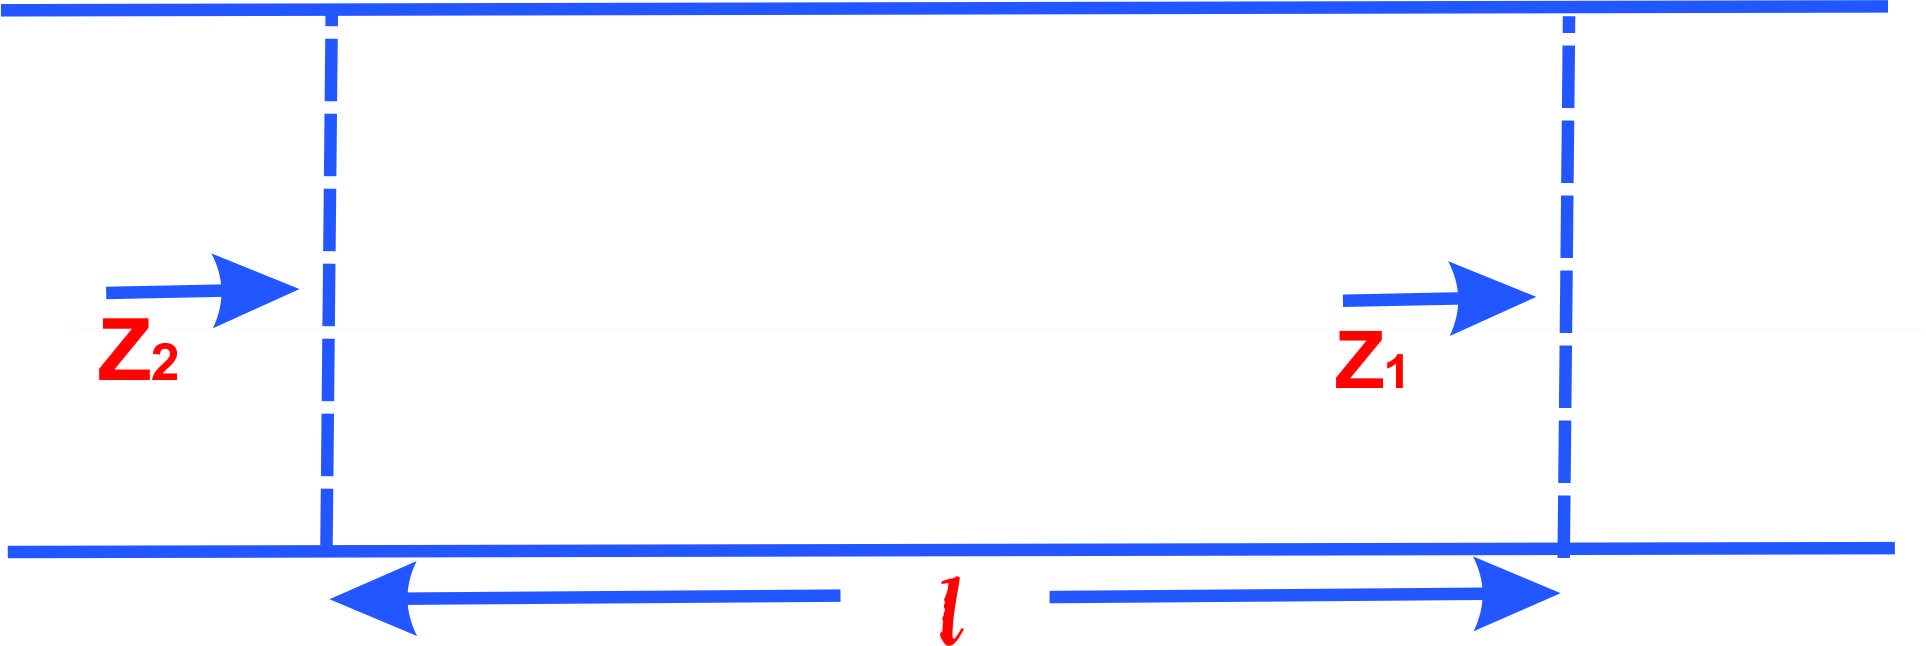
\includegraphics[scale=0.45]{./graphics/1234}
\caption{General representation of a transmission line}
\end{figure}

Recall from Equation~\ref{eqn:imp},
\begin{align*}
Z(l) = Z_0\left[\frac{Z_L\cosh(\gamma l) + Z_0\sinh(\gamma l)}{Z_L\sinh(\gamma l) + Z_0\cosh(\gamma l)}\right]
\end{align*}
Here, $Z_L = Z_1$ and $Z(l) = Z_2$.\\
\begin{align}
Z_2 = Z_0\left[\frac{Z_1\cosh(\gamma l) + Z_0\sinh(\gamma l)}{Z_1 \sinh(\gamma l) + Z_0 \cosh(\gamma l)}\right]
\label{eqn:z2norm}
\end{align}
Dividing both sides by $Z_0$
\begin{align*}
\frac{Z_2}{Z_0} = \frac{Z_0}{Z_0} \left[\frac{Z_1\cosh(\gamma l) + Z_0\sinh(\gamma l)}{Z_1 \sinh(\gamma l) + Z_0 \cosh(\gamma l)}\right]
\end{align*}
Divide the numerator and denominator by $Z_0$
\begin{align*}
\frac{Z_2}{Z_0} = \left[\frac{\frac{Z_1}{Z_0}\cosh(\gamma l) + \frac{Z_0}{Z_0}\sinh(\gamma l)}{\frac{Z_1}{Z_0}\sinh(\gamma l) + \frac{Z_0}{Z_0}\cosh(\gamma l)}\right]
\end{align*}
\begin{align*}
\bar{Z}_2 = \left[\frac{\frac{Z_1}{Z_0}\cosh(\gamma l) + \sinh(\gamma l)}{\frac{Z_1}{Z_0}\sinh(\gamma l) + \cosh(\gamma l)}\right]
\end{align*}
\begin{align*}
\bar{Z}_2 = \left[\frac{\bar{Z}_1\cosh(\gamma l) + \sinh(\gamma l)}{\bar{Z}_1\sinh(\gamma l) + \cosh(\gamma l)}\right]
\end{align*}
From Equation~\ref{eqn:z2norm} we can also invert the relationship to get $Z_1$ from $Z_2$ by cross multiplying.
\begin{align*}
Z_2 = Z_0\left[\frac{Z_1\cosh(\gamma l) + Z_0\sinh(\gamma l)}{Z_1 \sinh(\gamma l) + Z_0 \cosh(\gamma l)}\right]
\end{align*}
\begin{dmath*}
Z_2\left[Z_1\sinh(\gamma l) + Z_0\cosh(\gamma l)\right] = Z_0\left[Z_1\cosh(\gamma l) + Z_0\sinh(\gamma l)\right]
\end{dmath*}
\[Z_1Z_2\sinh(\gamma l) + Z_0Z_2\cosh(\gamma l) = Z_0Z_1\cosh(\gamma l) + Z_0^2\sinh(\gamma l)\]

Collect like terms and factorise out $Z_1$ on the left and $Z_0$ on the right-hand side of the equation
\begin{dmath*}
Z_1Z_2\sinh(\gamma l) - Z_1Z_0\cosh(\gamma l) = Z_0^2\sinh(\gamma l) - Z_0Z_2\cosh(\gamma l)
\end{dmath*}
\begin{dmath*}
Z_1\left[Z_2\sinh(\gamma l) - Z_0\cosh(\gamma l)\right] = Z_0\left[Z_0\sinh(\gamma l) - Z_2\cosh(\gamma l)\right]
\end{dmath*}
Make $Z_1$ the subject of the formula
\begin{align}
Z_1 = Z_0\left[\frac{Z_0\sinh(\gamma l) - Z_2\cosh(\gamma l)}{Z_2\sinh(\gamma l) - Z_0\cosh(\gamma l)}\right]
\label{eqn:z2norminv}
\end{align}
Multiply the numerator and denominator of Equation~\ref{eqn:z2norminv} by $-1$.
\begin{align*}
Z_1 = Z_0\left[\frac{Z_2\cosh(\gamma l) - Z_0\sinh(\gamma l)}{Z_0\cosh(\gamma l) - Z_2\sinh(\gamma l)}\right]
\end{align*}
Recall:
\begin{align*}
\cosh(\gamma l) = \cosh((-\gamma) l)
\end{align*}
\begin{align*}
\sinh(\gamma l) = -\sinh((-\gamma) l)
\end{align*}
So that,
\begin{align*}
\sinh((-\gamma) l) = -\sinh(\gamma l)
\end{align*}
So, equation~\ref{eqn:imp} can be used to transform impedance between $Z_1$ and $Z_2$ knowing the positive $l$ direction is from load towards the generator.

Now we go to a special case of the transmission lines.

\section{Lossless Transmission Line}
In practice, we want to transfer maximum power from the generator to the load. However, some losses occur in real transmission lines due to ohmic resistances. Every effort is usually made to make sure maximum power is delivered to the load by minimizing their losses. Hence, a good transmission line loss should be very small at its operating frequency. 

Once we have this condition in practice, then we can make some simplification to the transmission line problem and come up with an idea of what is called a \textbf{lossless transmission line}; whose ideal loss is zero.

The transmission line has four parameters $R, L, G$ and $C$ all in per unit length. $R$ and $G$ are ohmic values in the primary constant, that is, the resistance between the two ends of the conductors and the leakage current in the dielectric separating the two conductors respectively. Hence, power-losing elements exist because of the resistance and conductance. The inductance and capacitance exchange energy between themselves but does not result in any loss. Ideally, a line will be lossless if $R = G = 0$.

Substituting $R$ and $G$ as Zero in the propagation constant equation,
\begin{align*}
\gamma = \sqrt{(R + \jmath\omega L)(G + \jmath\omega C)}
\end{align*}
\begin{align*}
= \sqrt{(\jmath\omega L)(\jmath\omega C)}
\end{align*}
\begin{align*}
\gamma = \jmath\omega\sqrt{LC}
\end{align*}
Also,
\begin{align*}
\gamma = \alpha + \jmath\beta
\end{align*} 
Therefore,
\begin{align*}
\alpha + j\beta = \jmath\omega\sqrt{LC}
\end{align*}
so,
\begin{align*}
\alpha = 0, \beta = \omega\sqrt{LC}
\end{align*}

With no loss, there is no reason for the wave amplitude to reduce on the transmission line since $\alpha = 0$(The Attenuation Constant). Hence, there is a sustained propagation of electromagnetic waves along the transmission line.\\
$\beta = \omega\sqrt{LC}$ but $\beta = \frac{2\pi}{\lambda}$ and $\omega = 2\pi f $. That is,
\begin{align*}
\frac{2\pi}{\lambda} = 2\pi f\sqrt{LC}
\end{align*}
$2\pi$ will cancel out to give,
\begin{align*}
\frac{1}{\lambda} =  f\sqrt{LC}
\end{align*}
Recall, $\lambda f = V$ which is the velocity of the wave in the transmission line.
\begin{align*}
\lambda f = \frac{1}{\sqrt{LC}} = V
\end{align*}
The velocity of the wave in the transmission line is related to the inductance and capacitance of the transmission line. Hence the velocity is fixed once the inductance and capacitance are given.

Can we vary load $L$ and $C$ to vary $V$? Not really, $L$ and $C$ are coupled. Varying $C$ changes $L$ and varying $L$ changes $C$ to make $V$ a constant of the transmission line. The velocity parameter is decided by the field condition in the transmission line and is fixed by the boundary condition. 

For instance, with varying separation between the two conductors, the mutual inductance will vary and at the same time, the separation between the two conductors vary thereby varying the capacitance. Hence, $L$ and $C$ of the transmission line are not independent quantities.

We then calculate the characteristic impedance on a lossless transmission line which is given as,
\begin{align*}
Z_0 = \sqrt{\frac{R + \jmath\omega L}{G + \jmath\omega C}} = \sqrt{\frac{\jmath\omega L}{\jmath\omega C}} = \sqrt{\frac{L}{C}}.
\end{align*}
Which is a real quantity. So, for a lossless line, $Z_0$ is REAL. We do not have any ohmic resistance or conductance in the line and yet it is at this point we have a characteristic impedance that is real. That is, Pure ohmic. Hence, the wave which travels forward or backwards always sees a characteristic impedance that is a real impedance like resistance. This makes sense since you have a line carrying only forward waves which will go forever and no energy is reflected. 

That is, power somewhere is going to get dumped. So if we have a real quantity for $Z_0$, it means that power is completely transferred to the line; it does not mean that power is lost in the line. So for a lossless line, if the impedance on the line is measured, something more like resistance will be measured.

Now, we go to a case where little loss is accepted in the transmission line and then find the derivations for $\gamma$ and $Z_0$.
\section{Low-loss Transmission Line}
$R \ll \omega L$, $G \ll \omega C$ are the two conditions for a low-loss transmission line. Using the propagation constant equation, we have:
\begin{align*}
\gamma = \sqrt{(R + \jmath\omega L)(G + \jmath\omega C)}
\end{align*}
Which is the same as,
\begin{align*}
\gamma = \sqrt{{(\jmath\omega L)(\jmath\omega C)(1 + \frac{R}{\jmath\omega L})(1 + \frac{G}{\jmath\omega C})}}
\end{align*}
where $\frac{1}{\jmath} = -\jmath$, we have that $\gamma$ is
\begin{align}
= \sqrt{{(\jmath\omega L)(\jmath\omega C)(1 - j\frac{R}{\omega L})(1 - j\frac{G}{\omega C})}}
\label{eqn:lowlossgamma}
\end{align}

Recall from Binomial expansion the a power series with fraction power can be expressed as follows where x is the fractional part. 
\begin{dmath*}
(1 + x)^{\frac{1}{2}} = \Comb{\frac{1}{2}}{0}(1)^{\frac{1}{2}}x^0 + \Comb{\frac{1}{2}}{1}(1)^{{\frac{1}{2}} - 1}x^1 + \ldots
\end{dmath*}
Where $\Comb{\frac{1}{2}}{0}(1)^{\frac{1}{2}}x^0 = 1$ and $\Comb{\frac{1}{2}}{1}(1)^{\frac{1}{2} - 1}x = \Comb{\frac{1}{2}}{1}(1)x$.

Let's expand the combination $\Comb{\frac{1}{2}}{1} x$
\begin{dmath*}
\Comb{\frac{1}{2}}{1} x = \begin{pmatrix}\frac{1}{2}\\1 \end{pmatrix}x = \frac{\frac{1}{2}! x}{(\frac{1}{2} - 1)!1!} = \frac{\frac{1}{2}(\frac{1}{2} - 1)! x}{(\frac{1}{2} - 1)!1!} = \frac{1}{2}x
\end{dmath*}

Thus,
\[(1 + x)^{\frac{1}{2}} = 1 + \frac{1}{2}x + \ldots\]
and
\[(1 - x)^{\frac{1}{2}} = 1 - \frac{1}{2}x + \ldots\]

Hence from the Equation~\ref{eqn:lowlossgamma}
\[jw\sqrt{LC}\left(1 - \frac{\jmath R}{wL}\right)^{\frac{1}{2}}\left(1 - \frac{\jmath G}{wC}\right)^{\frac{1}{2}}\]
Let $x = \frac{\jmath R}{\omega L}$ and $x' = \frac{\jmath G}{\omega C}$
\begin{dmath*}
(1 - \frac{\jmath R}{\omega L})^{\frac{1}{2}} = 1 - \frac{1}{2}\frac{\jmath G}{\omega C} + \ldots
\end{dmath*}
and
\begin{dmath*}
(1 - \frac{jG}{\omega C})^{\frac{1}{2}} = 1 - \frac{1}{2}\frac{\jmath R}{\omega L} + \ldots 
\end{dmath*}
Thus, Equation~\ref{eqn:lowlossgamma} becomes
\begin{dmath*}
\gamma = jw\sqrt{LC}\left(1 - \jmath \frac{R}{2\omega L} + \ldots\right)\left(1 - j\frac{G}{2\omega C} + \ldots\right) = jw\sqrt{LC} \left[1- \left(\frac{\jmath R}{2\omega L}\right) - \left(\frac{\jmath G}{2\omega C}\right) + \left(\frac{\jmath R}{2\omega L}\right)\left(\frac{\jmath G}{2\omega C}\right)\right]
\end{dmath*}
Recall that two combination terms were used earlier because of the complex variable $\frac{jR}{wL}$ and $\frac{\jmath G}{\omega C}$, the product of $\frac{\jmath R}{2\omega C}$ and $\frac{\jmath G}{2\omega L}$ tends to zero since $R \ll wL$ and $G \ll \omega C$ for a low loss transmission line.

Thus,
\begin{dmath}    
\gamma = \jmath\omega\sqrt{LC} \left[1- \frac{\jmath R}{2\omega L} - \frac{\jmath G}{2\omega C}\right] = \jmath\omega\sqrt{LC} - \jmath\frac{R}{2\omega L}\left(\jmath\omega\sqrt{LC}\right) - j\frac{G}{2\omega C}\left(\jmath\omega\sqrt{LC}\right)
\end{dmath}
Expressing $L = \sqrt{L} \times \sqrt{L}$ and $C = \sqrt{C} \times \sqrt{C}$, we have
\begin{dmath*}
\gamma = \jmath\omega\sqrt{LC} + \frac{R\sqrt{L}\sqrt{C}}{2\sqrt{L}\sqrt{L}} + \frac{G\sqrt{L}\sqrt{C}}{2\sqrt{C}\sqrt{C}} = \jmath\omega\sqrt{LC} + \frac{1}{2}R\sqrt{\frac{C}{L}} + \frac{G}{2}\sqrt{\frac{L}{C}} 
\end{dmath*}

Recall that $\gamma = \alpha + j\beta$, therefore,
\begin{align*}
\jmath\omega\sqrt{LC} + \frac{1}{2}R\sqrt{\frac{C}{L}} + \frac{G}{2}\sqrt{\frac{L}{C}} = \alpha + \jmath\beta
\end{align*}
So,
\begin{align}
\alpha &= \frac{1}{2}R\sqrt{\frac{C}{L}} + \frac{1}{2}G\sqrt{\frac{L}{C}}\label{eqn:lowlossalpha}\\
\beta &= \omega\sqrt{LC}
\end{align}
Compared to the lossless transmission line where $\alpha = 0$, there is a value for the attenuation constant. Also, we have that $\beta = \omega\sqrt{LC}$ for both cases of lossless and low-loss, which means that the phase constant does not change when we introduce low-loss to the transmission line. Hence, if we are interested in only the phase constant for a low-loss line, it can be treated as a lossless transmission line. However, for a real line $\alpha \neq 0$, there is that small loss so that as you travel the wave, amplitude reduces slowly at $e^{-\alpha}$.

Recall, $Z_0 = \sqrt{\frac{L}{C}}$ for a lossless line, substituting it in Equation~\ref{eqn:lowlossalpha}, we have,
\[\alpha = \frac{1}{2}R\sqrt{\frac{C}{L}} + \frac{1}{2}G\sqrt{\frac{L}{C}} = \frac{1}{2}(\frac{R}{Z_0} + GZ_0)\]
Therefore,
\[\gamma = \jmath\omega\sqrt{LC} + \frac{1}{2}(\frac{R}{Z_0} + GZ_0)\]
So if $R$ and $G$ are known and $Z_0$ for the lossless line has been determined, we can use $\alpha = \frac{1}{2}(\frac{R}{Z_0} + GZ_0)$ to calculate $\alpha$ for the low-loss line.
\begin{align*}
Z_0 = \sqrt{\frac{R + \jmath\omega L}{G + \jmath\omega C}} = \sqrt{\frac{\jmath\omega L(1 - \jmath\frac{R}{\omega L})}{\jmath\omega C(1 - \jmath\frac{G}{\omega C})}}
\end{align*}
$jw$ will cancel out, leaving us with
\begin{align*}
\sqrt{\frac{L}{C}}\sqrt{\frac{1 - j\frac{R}{\omega L}}{1 - j\frac{G}{\omega C}}} =\sqrt{\frac{L}{C}}\left(1 - \jmath\frac{R}{\omega L}\right)^{\frac{1}{2}}\left(1 - \jmath\frac{G}{\omega C}\right)^{-\frac{1}{2}} 
\end{align*}
From Binomial expansion, we have that:
\begin{align*}
Z_0 = \sqrt{\frac{L}{C}}\left(1 - \jmath\frac{R}{2\omega L} + \ldots\right)\left(1 - \jmath\frac{G}{2\omega C} + \ldots\right)
\end{align*}
\begin{align*}
= \sqrt{\frac{L}{C}}\left(1 - \jmath\frac{R}{2\omega L} - \jmath\frac{G}{2\omega C} + \text{\ldots smaller terms}\right)
\end{align*}
The characteristic impedance is no more real but complex. Its real value is the same as that of a lossless line. We have a small imaginary part which implies the presence of losses in the transmission line.

From now on, when given a transmission line problem, we assume it to be lossless unless we are told specifically that the line is lossy.

\newpage
\section*{Exercises}
\begin{ExerciseList}
\Exercise[label={ex41}]
Show that for a lossless transmission line, the velocity of the wave is a function of L and C i.e. $\left(v = \frac{1}{\sqrt{LC}}\right)$.

\Exercise[label={ex42}]
Prove that for both a lossless and a low-loss transmission line, the phase constant remains the same while the attenuation constant changes.
\end{ExerciseList}
%\chapter{\textbf{Standing Wave Pattern}}
In the previous chapter, we introduced the concept of a lossless transmission line ( i.e a line is lossless if $R=G=0$). We also introduced the concept of a low-loss transmission line which is a more practical line, i.e $R \ll \omega L$, $G \ll \omega C $.\\

In this chapter, we would study the conditions for treating the transmission line as low-loss at a particular frequency, the variation of voltage and current along a transmission line, the concept of voltage standing wave ratio (VSWR), the condition for full reflection at the load end, the relationship between $R_{max}$ and VSWR and also the relationship between $R_{min}$ and VSWR.
\section{Low-loss Transmission Line at a Particular Frequency.}
From our previous chapter, we recall that,
\begin{equation}
\gamma = \frac{1}{2}R\sqrt{\frac{C}{L}} + \frac{G}{2}\sqrt{\frac{L}{C}} +\jmath\omega\sqrt{LC}
\label{eqn:refcoeffient1}
\end{equation}
which states the conditions defined for a low-loss transmission line in terms of the primary constants(R, L, C and G) of the line. To treat a line as a low-loss transmission line, one will have to express these conditions ( $R \ll \omega L$ and $G \ll \omega C$ ) in terms of the secondary parameters ( $\alpha$ and $\beta $) since these parameters are readily available on the data-sheet. If we can establish a relationship between these parameters ( $\alpha$ and $\beta $) for the low-loss nature of the line, then we can find out whether a particular line is low-loss at a particular frequency.\\
Recall that,
\begin{equation}
\gamma = \alpha + \jmath\beta
\label{eqn:refcoeffient2}
\end{equation}
comparing equation~\ref{eqn:refcoeffient1} with equation~\ref{eqn:refcoeffient2}, we have that;
 
\begin{equation}
\alpha = \frac{1}{2}R\sqrt{\frac{C}{L}} + \frac{1}{2}G\sqrt{\frac{L}{C}}	
\label{eqn:attenconst}
\end{equation}
\begin{align}
\beta = \omega\sqrt{LC}
\end{align}
Since we have expressed equation~\ref{eqn:refcoeffient1} in terms of secondary constants, let's find out under what condition the transmission line can be treated as low-loss.\\
From equation~\ref{eqn:attenconst} we have,

\begin{equation*}
\alpha =\frac{1}{2}R\sqrt{\frac{C}{L}} + \frac{1}{2}G\sqrt{\frac{L}{C}}	
\end{equation*}\\
Multiplying the numerator and denominator of the first term by $\sqrt{\frac{L}{L}}$ and the second term by $\sqrt{\frac{C}{C}}$ , we get ;
\begin{equation*}
\alpha = \frac{1}{2} R \sqrt{\frac{C}{L}} \sqrt{\frac{L}{L}} + \frac{1}{2} G \sqrt{\frac{L}{C}} \sqrt{\frac{C}{C}} 
\end{equation*}\\
\begin{equation*}
\alpha =  \frac{1}{2} R \sqrt{\frac{CL}{L^2}} + \frac{1}{2} G \sqrt{\frac{LC}{C^2}}	
\end{equation*}\\
\begin{equation*}
\alpha = \frac{1}{2} \frac{R}{L} \sqrt{LC} + \frac{1}{2} \frac{G}{C} \sqrt{LC}
\end{equation*}\\
Multiplying numerator and denominator by $\omega$\\
\begin{equation*}
\alpha = \frac{1}{2} \frac{R}{\omega L} \omega \sqrt{LC} + \frac{1}{2} \frac{G}{\omega C} \omega \sqrt{LC}
\end{equation*}
\begin{equation*}
\alpha = \frac{1}{2} \omega\sqrt{LC}{(\frac{R}{\omega L} + \frac{G}{\omega C}})
\end{equation*}
But $\beta = \omega \sqrt{LC}$\\
\begin{equation}
\alpha = \beta\frac{1}{2} ( \frac{R}{\omega L} + \frac{G}{\omega C})
\end{equation}
Recall that for low-loss, $R \ll \omega L$ and $G \ll \omega C$\\
$\frac{R}{\omega L} \ll 1$ and $\frac{G}{\omega C} \ll 1$\\
Therefore,  $\frac{1}{2} (\frac{R}{\omega L} + \frac{G}{\omega C}) \ll 1$\\

$\alpha = \beta \;\; \times$ (something far smaller than 1).\\
Hence, for a low-loss transmission line, $\alpha \ll \beta$ where $\beta = \frac{2 \pi}{\lambda}$.
Considering a wave which travels a distance of one wavelength along the transmission line, its phase change$(\beta)$ becomes $2\pi$ i.e $\beta= 2 \pi$, then the amplitude of the wave varies by:
\begin{equation*}
e^{-\alpha x} = e^{-\alpha \lambda}	
\end{equation*}
Where $\lambda = \frac{2 \pi}{\beta}$
\begin{equation*}
e^{- \alpha x} = e^{-\alpha \frac{2 \pi}{\beta}}
\end{equation*}
Since for a low-loss transmission line $\alpha<<\beta$, therefore the quantity $e^{-\alpha \frac{2 \pi}{\beta}} \ll 1$.\\\\
Hence, amplitude reduction is very small as the original amplitude is close to the final amplitude. So, a line can be treated as a low-loss transmission line if the change in amplitude over one wavelength is negligibly small. Let our negligibly small be 1 per cent.\\\\ 
$\frac{\alpha 2 \pi}{\beta} \approx \frac{1}{100}$, $ e^{-0.01} = 0.99005$ of the initial value.\\\\
The wave amplitude only reduces by $1-0.99005=0.00995$ or 1 per cent. That means the wave amplitude only reduces by 1 per cent after a distance of 1 wavelength.\\\\
A line can be treated as a low-loss transmission line if $\alpha \ll \beta$ depending on the given frequency but if the frequency changes such that $\alpha \geq \beta$, the line cannot be treated as a low-loss transmission line.\\

\begin{exmp}
Let's say we have a transmission line with $L = 0.25\mu H/m$, ${C= 100pF/m}$, $G = 0$, what is the resistance of the transmission line so that the line can be treated as a low-loss transmission line given the frequency of operation as $100MHz$ ?\\\\
\textbf{Solution}:\\
$L= 0.25\mu H/m$, $C= 100pF/m$, $G = 0$\\
$\beta = 2\pi \ f {\sqrt{LC}}$
\begin{equation*}
=2 \pi \times 10^8 \sqrt{(0.25 \times 10^{-6}) \times (100 \times 10^{-12})}  = \pi rad/m
\end{equation*}\\
 For a low-loss transmission line, taking 1 percent of $\beta$,
$ \alpha= \frac{1}{100} \beta = \frac{\pi}{100}$.\\\\
Also,
\begin{equation*}
\alpha = \beta\frac{1}{2} ( \frac{R}{\omega L} + \frac{G}{\omega C})
\end{equation*}\\
Given that, G=0\\
\begin{equation*}
\alpha = \beta\frac{1}{2} ( \frac{R}{\omega L} )
\end{equation*}\\
Recall that $\beta = \omega\sqrt{LC} $, now we get :
\begin{equation*}
\alpha = \frac{1}{2}\frac{R}{\omega L} \times \omega\sqrt{LC} 
\end{equation*}
\begin{equation*}
\alpha = \frac{1}{2} R \sqrt \frac{LC}{L^{2}} 
\end{equation*}\\
\begin{equation*}
\alpha = \frac{1}{2} R \sqrt \frac{C}{L}
\end{equation*}
\begin{equation*}
\frac{\pi}{100} = \frac{1}{2} R \sqrt{\frac{100 \times 10^{(-12)}}{0.25 \times 10^{(-6)}}}
\end{equation*}
\begin{equation*}
 R=\pi\Omega/m.
\end{equation*}\\
 If $R \leq \pi\Omega/m$, the line is low-loss at $ f= 100MHz$. If the frequency changes, the line may not satisfy this low-loss condition, hence we have to check again.
\end{exmp}

Therefore, unless you are specifically told that a line is a lossy line, we are at liberty to treat the line as a lossless line since the phase constant as we have seen for lossy and lossless lines are the same. Also, the characteristics impedance of a low-loss line is almost real and the same as the characteristics impedance of a lossless line. So unless we are specifically told the line is lossy, we shall default to treating transmission line problems as lossless and carry out all analysis for a lossless transmission line. Hence for all transmission line problems, we consider it lossless so that, 
\begin{align*}
Z_0 = \sqrt{{\frac{\jmath\omega L}{\jmath\omega C}}} = \sqrt{\frac{L}{C}} = real , \quad \quad \gamma= \jmath\beta = \jmath\omega\sqrt{LC}
\end{align*}
  
\section{Voltage And Current Variation on Transmission Line}

Revisiting the general voltage and current expression of the transmission line with origin  at the load point, we have:
\begin{equation}
V =  V^+ e^{- \gamma x} + V^- e^{\gamma x}
\label{eqn:genvoltage}
\end{equation}
\begin{equation}
I= \frac{V^+}{Z_o} e^{- \gamma x} - \frac{V^-}{Z_o} e^{\gamma x}
\label{eqn:gencurrent}
\end{equation}
\begin{figure}[h]
\centering
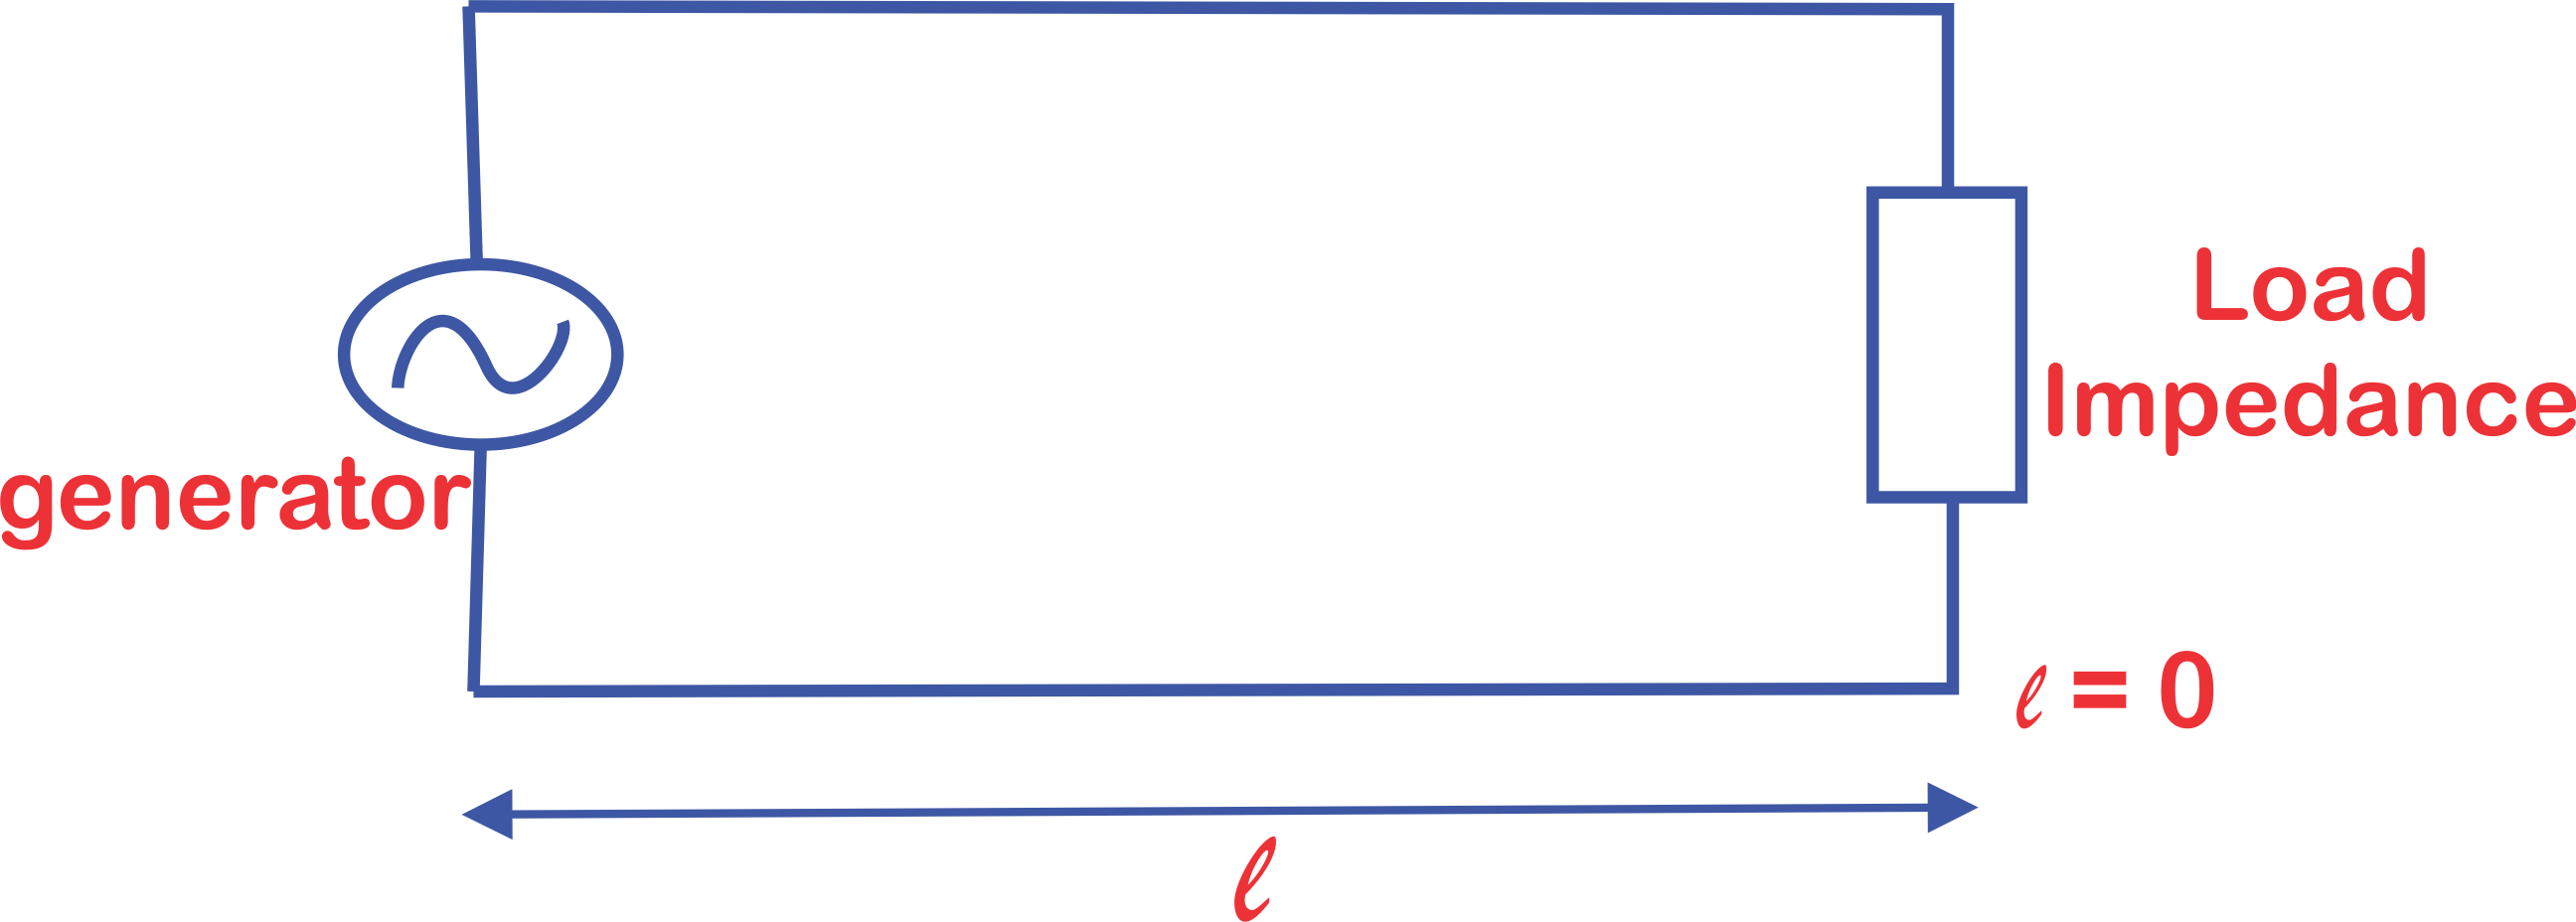
\includegraphics[width=0.7\linewidth]{./graphics/11111111}
\caption{Wave moving towards the Generator}
\label{fig:11111111}
\end{figure}

For a lossless transmission line at any point $l$,\\
substituting $\gamma = \jmath\beta$ and $x=-l$ into equation~\ref{eqn:genvoltage} , we have ;
\begin{equation*}\\
V(l) = V^+ e^{j \beta l} + V^- e^{- j \beta l}
\end{equation*}\\
Divide through by $ V^+ e^{j \beta l}$, we get ;\\
\begin{equation*}
\frac{V(l)}{ V^+ e^{j \beta l}}= (1 +\frac{V^- e^{- j \beta l}}{V^+ e^{j \beta l}})
\end{equation*}\\
\begin{equation*}
V(l) = V^+ e^{j \beta l}(1+ \frac{V^-}{V^+}e^{-j 2 \beta l})
\end{equation*}\\
\begin{equation}
V(l) = V^+ e^{j \beta l}(1 + \Gamma_L e^{-j 2 \beta l})
\label{eqn:voltagefromload}
\end{equation}
where $\Gamma _L = \frac{V^-}{V^+}$. Similarly, substituting $\gamma = j\beta$ and $x = -l$ into equation~\ref{eqn:gencurrent}:
\begin{equation*}
I(l) = \frac{V^+}{Z_o}  e^{\jmath \beta l} - \frac{V^-}{Z_o} e^{-\jmath\beta l}
\end{equation*}
Divide through by $\frac{V^+}{Z_o}  e^{\jmath\beta l}$
\begin{equation*}
\frac{I(l)}{\frac{V^+}{Z_o}  e^{\jmath\beta l}} =( 1- \frac{\frac{V^-}{Z_o} e^{-\jmath\beta l}}{\frac{V^+}{Z_o}  e^{\jmath\beta l}} )
\end{equation*}
\begin{equation*}
\frac{I(l)}{\frac{V^+}{Z_o}  e^{\jmath\beta l}} =( 1-  \frac{V^-}{V^+}e^{-\jmath 2 \beta l})
\end{equation*}
\begin{equation}
I(l) = \frac{V^+}{Z_o}e ^{j \beta l}  \{ 1 - \Gamma_L e^{-j 2 \beta l}\}
\label{eqn:currentfromload}
\end{equation}
where,
\begin{equation*}
\Gamma _L = \frac{V^-}{V^+}
\end{equation*}
$V = f( V^{+}, V^{-})$ and $I = f(I^{+}, I^{-})$ means $V$ and $I$ are a superposition of forward and backward travelling wave, which is then a \textbf{Standing Wave}. 
\begin{equation}
\Gamma_L = |\Gamma_L|e^{j\phi_L}
\label{eqn:refcoefficientfromload}
\end{equation}
where $\phi_L =$ phase of the reflection coefficient at the load end. Then, we can write down the $V(l)$ and $I(l)$ explicitly in terms of the magnitude of the reflection coefficient and the phase.\\
Therefore substituting equation~\ref{eqn:refcoefficientfromload} into equations \ref{eqn:voltagefromload} and \ref{eqn:currentfromload} respectively, we will get ;
\begin{equation*}
V(l) = V^{+}e^{\jmath\beta l}(1 + |\Gamma_L|e^{j\phi_L} . e^{-j 2 \beta l})
\end{equation*}
\begin{equation}
V(l) = V^{+}e^{\jmath\beta l}(1 + |\Gamma_L|  e^{\jmath(\phi_L -2 \beta l)})
\end{equation}
Similarly,
\begin{equation*}
I(l) = \frac{V^+}{Z_o}e ^{j \beta l}( 1 - |\Gamma_L|e^{\jmath\phi_L} . e^{-\jmath 2\beta l})
\end{equation*}
\begin{equation}
I(l) = \frac{V^+}{Z_o}e ^{j \beta l}( 1 -|\Gamma_L|  e^{j(\phi_L -2 \beta l)})
\end{equation}
As we move from load to generator, $l$ increases positively, making $\phi_L -2 \beta l$ more and more negative. In the complex plane, when a phase gets more negative, it means we are moving in a clockwise direction.
\begin{figure}[h]
\centering
\includegraphics[width=0.9\linewidth]{./graphics/"473 drawings"}
\caption{Clockwise and Anticlockwise movement of l}
\label{fig:473-drawings}
\end{figure}

So by moving towards the generator, the phase becomes more and more negative, while the amplitude of $|\Gamma_L|$ remains constant. The total voltage is scaled by the vector sum of the real term (1) and complex term $|\Gamma_L|  e^{j(\phi_L -2 \beta l)}$. Hence, we have a summation of a real vector, whose magnitude is 1, plus a complex term shown below. 
\begin{figure}[h]
\centering
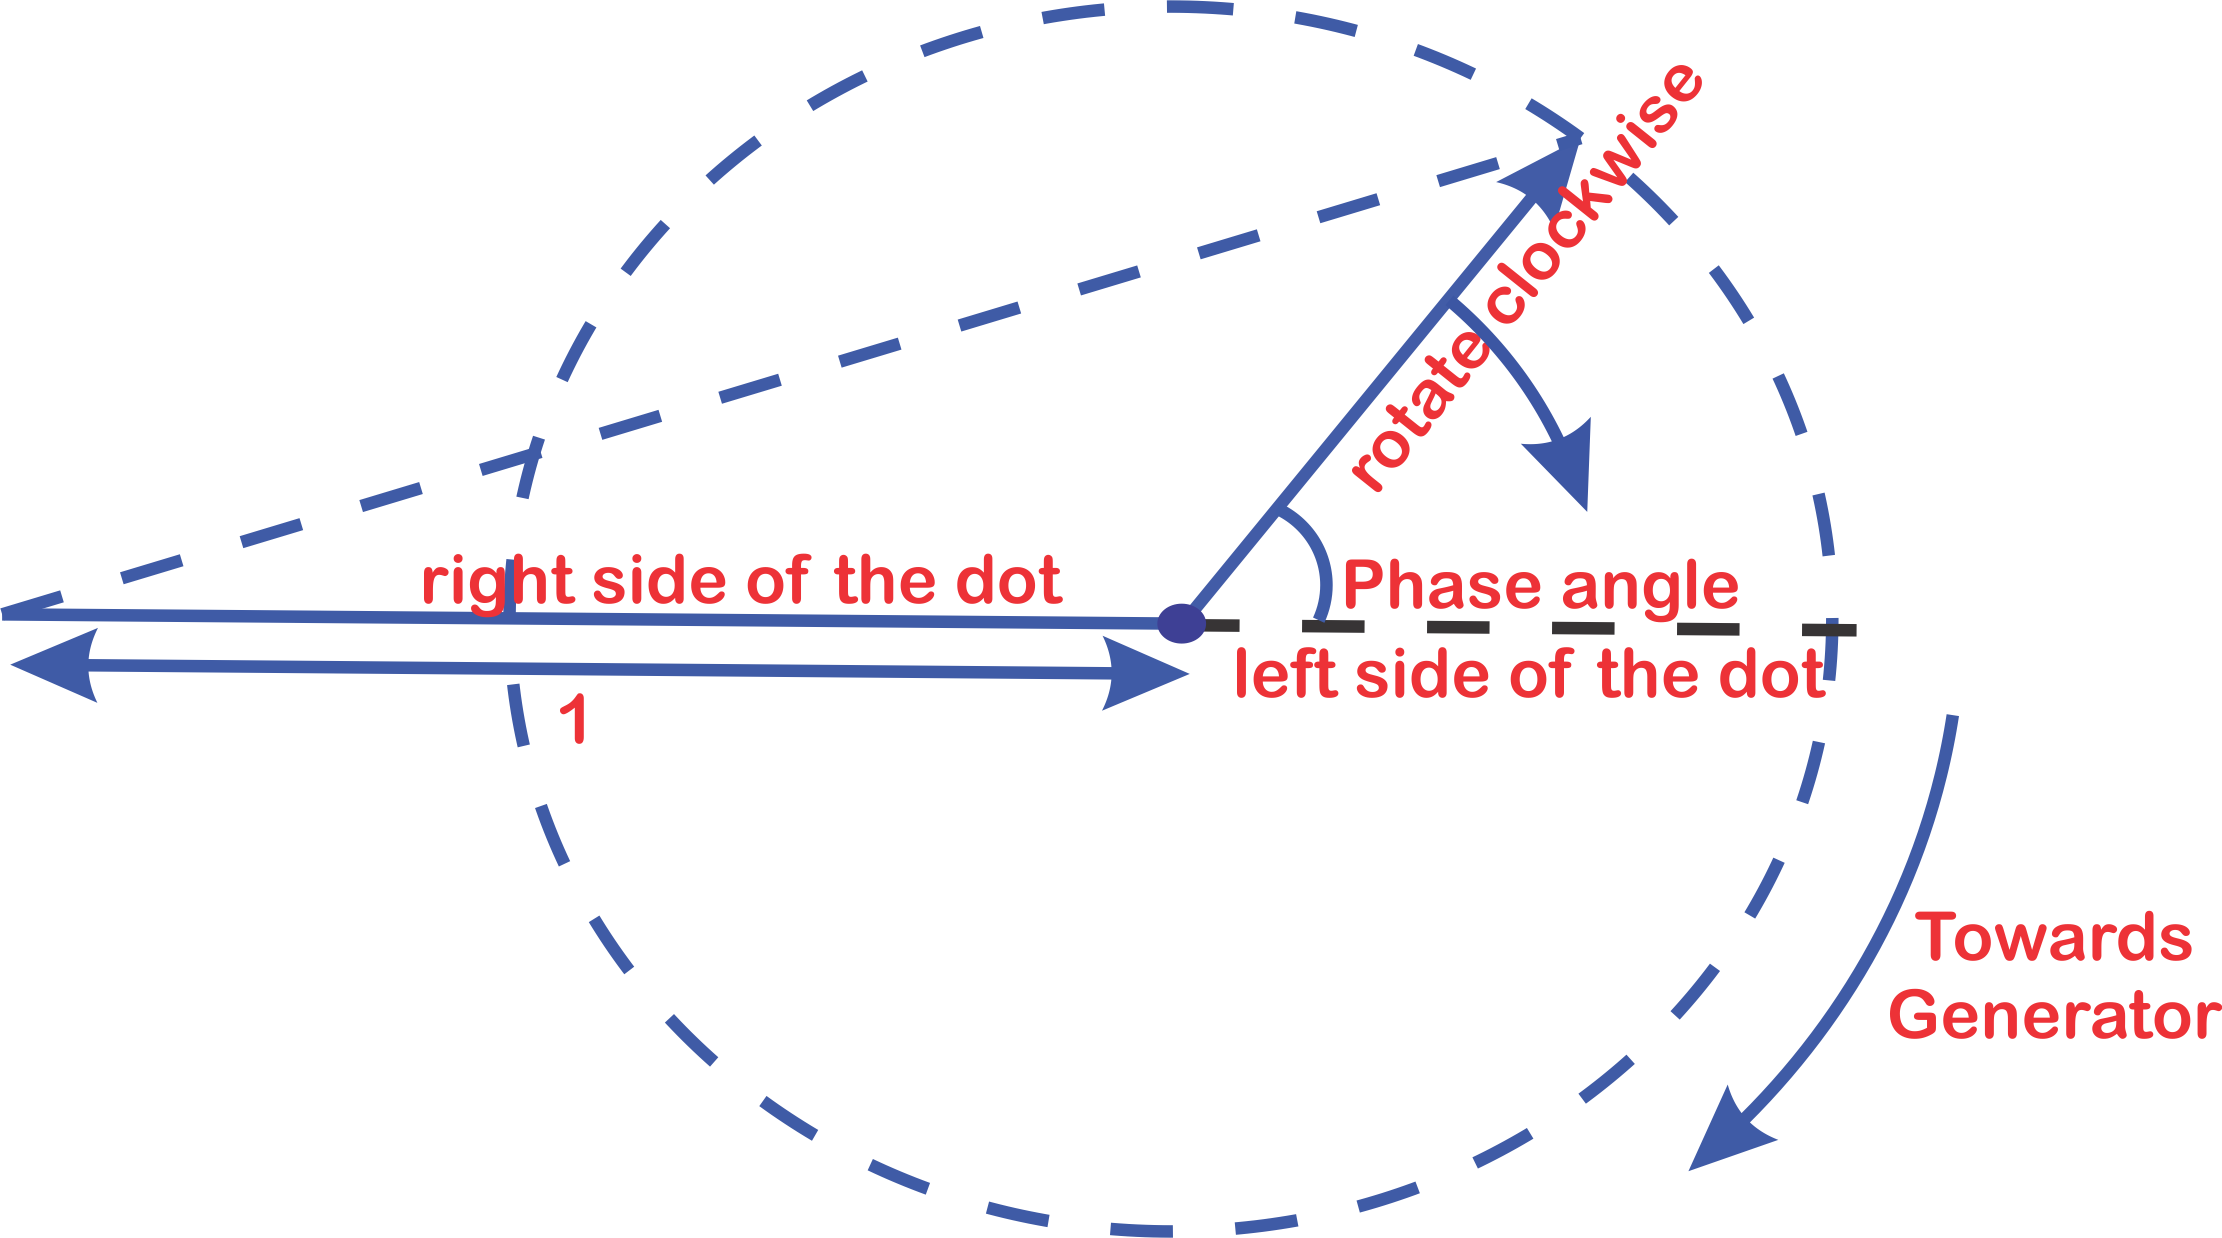
\includegraphics[width=0.6\linewidth]{./graphics/kjhgfdwert}
\caption{Argand Diagram}
\label{fig:kjhgfdwert}
\end{figure}

The magnitude $( 1+|\Gamma_L|  e^{j(\phi_L -2 \beta l)})$ varies as we move along the transmission line.\\
 From figure 5.3 \footnote{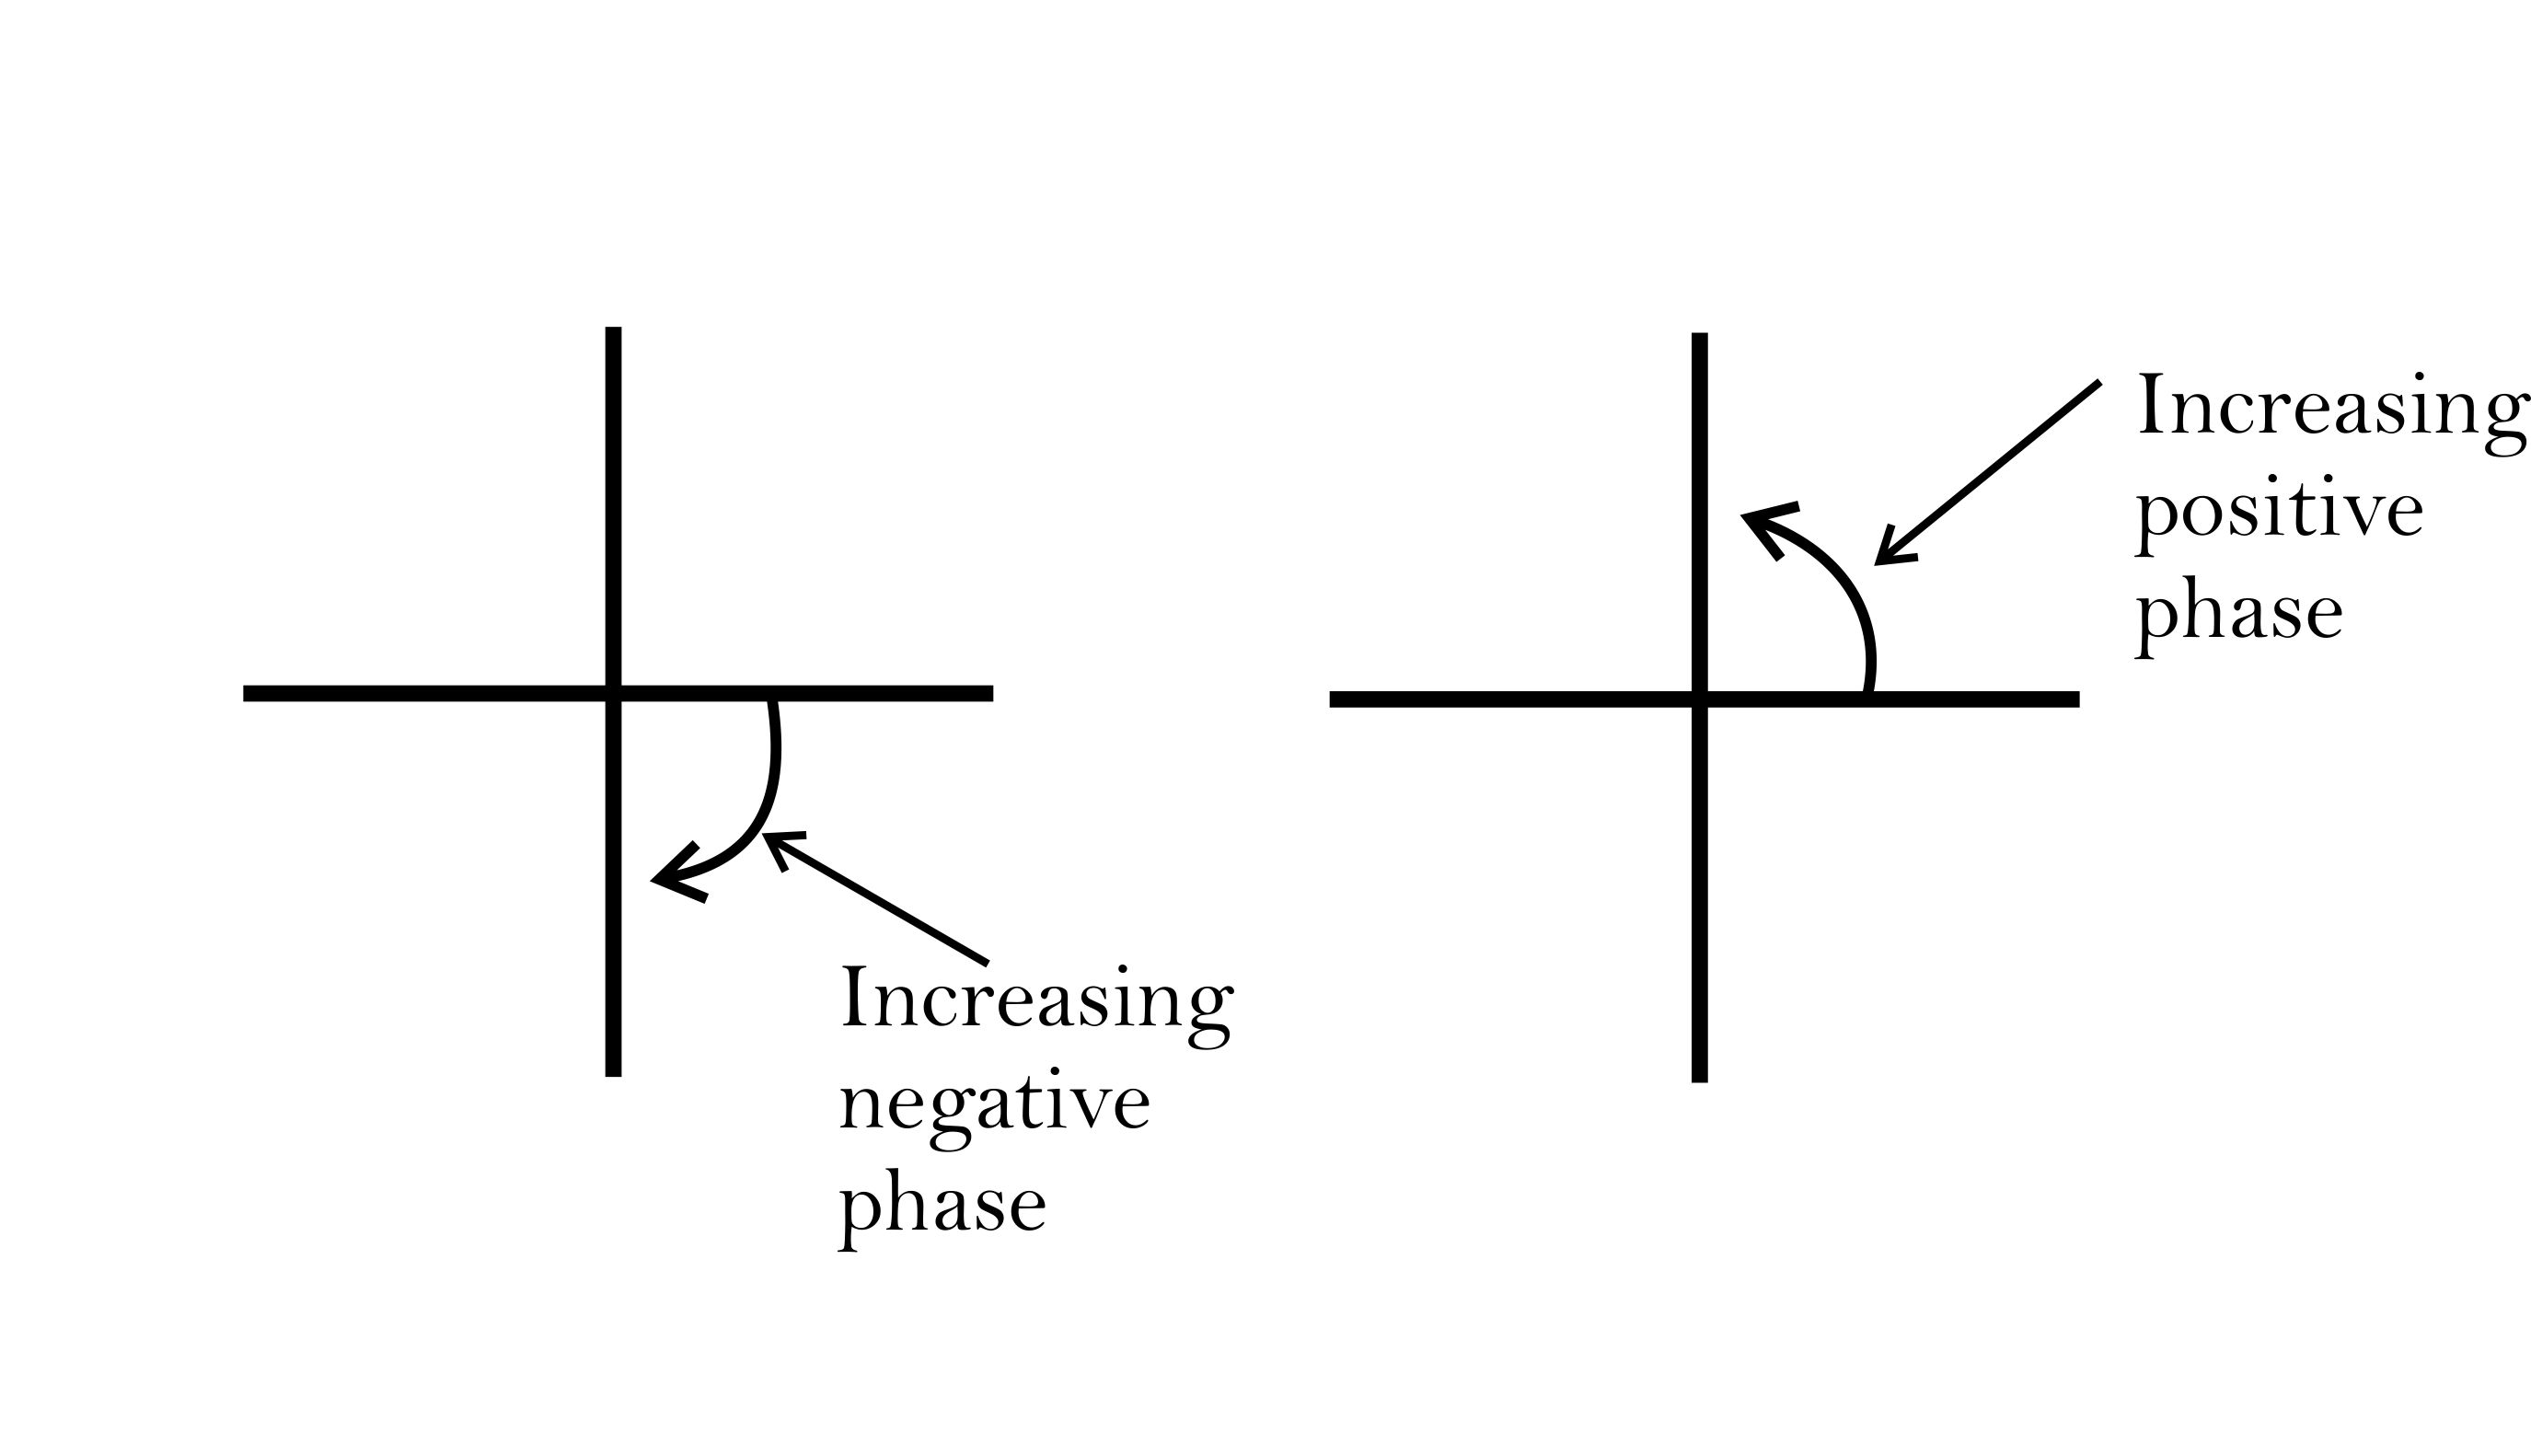
\includegraphics[scale=0.15]{./graphics/picture4} 

Argand Diagram refers to a geometric plot of complex numbers as points z = x+iy using the x-axis as the real axis and the y-axis as the imaginary axis. Such plots are named after Jean-Robert Argand(1768-1822), although they were first described by Norwegian-Danish land surveyor and mathematician Casper Wessel (1745-1818.)}Argand Diagram below, \\
$ A =| 1+| \Gamma_L| e^{j (\phi_L - 2\beta l)}|$ \quad$, B=| \Gamma_L|$\\\\
$Phase\ angle = \phi_L - 2 \beta l$.\\\\
If $ \phi_L - 2 \beta l = 2 \pi n$, where n is an integer, then $ e^{j(\phi_L - 2 \beta l)} = 1$. This is the right side of the dot on the real axis.\\\\ 
Also, if $\phi_L - 2 \beta l=(2 n + 1) \pi$, then $e^{j (\phi_L - 2 \beta l)} = -1$. This is the left side of the dot on the real axis.
\begin{equation*}
V(l) = V^{+}e^{j\beta l}(1 + |\Gamma_L|  e^{j(\phi_L -2\beta l)})
\end{equation*}
$(1 + |\Gamma_L|  e^{j(\phi_L -2\beta l)})$ add when they are in phase to give maximum V i.e at $(\phi_L -2\beta l) = 0, 2\pi, 4\pi ...$, and subtract to give minimum V i.e at  $(\phi_L -2\beta l) = \pi, 3\pi, 5\pi ...$ \\
This is opposite to the behaviour of the current relationship, when 1 and  $-|\Gamma_L|  e^{j(\phi_L -2\beta l)}$ in $1-|\Gamma_L|  e^{j(\phi_L -2\beta l)}$ are out of phase, they add at $\pi, 3\pi, 5\pi...$ to give maximum current and they cancel when in phase at $0, 2\pi, 4\pi...$, to give minimum current.\\
 As stated earlier, when $ e^{j(\phi_L - 2 \beta l)} = 1$, the voltage is maximum and the current is minimum. When $ e^{\jmath(\phi_L - 2 \beta l)} = -1$, the voltage is minimum and the current is maximum. So at the same location along the transmission line, maximum voltage corresponds to minimum current, and minimum voltage corresponds to maximum current. This is opposite to what we observed in a lumped circuit, where the maximum voltage point corresponds to maximum current and minimum voltage corresponds to minimum current.\\
The maximum voltage and current does not occur at the same point on the transmission line, they are staggered in space. Whenever there is a maximum voltage, there is a minimum current and vice versa. So the standing wave of voltage and current are shifted with respect to each other in space on the transmission line. 
\begin{figure}[h]
\centering
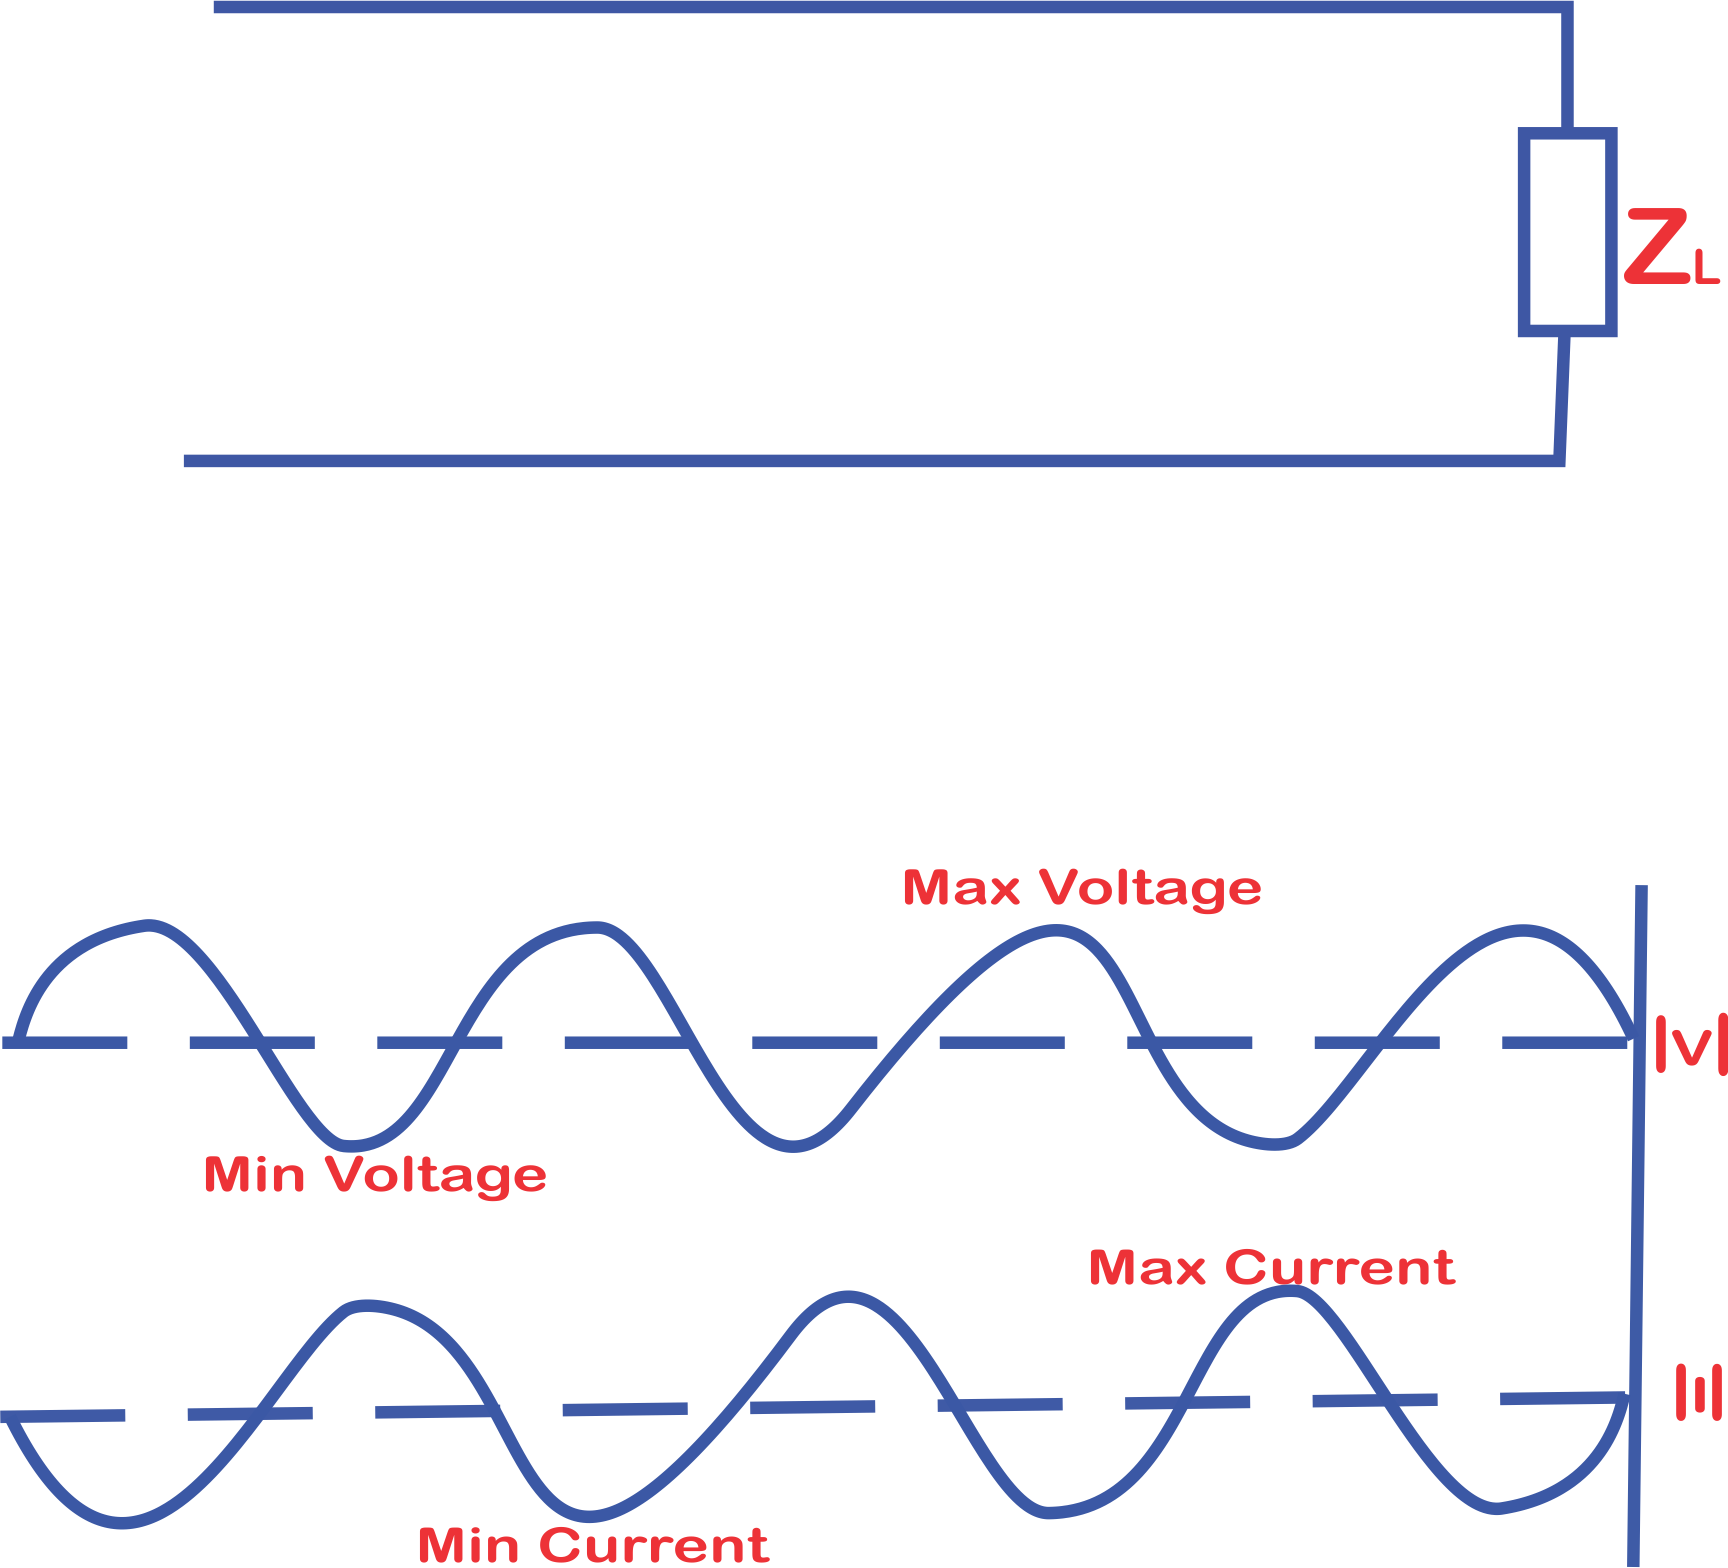
\includegraphics[width=0.6\linewidth]{./graphics/asdfghjhgfdsa}
\caption{Voltage and Current Plot, with Increasing l to the left}
\label{fig:asdfghjhgfdsa}
\end{figure}
From figure 5.4, we observe that maximum voltage corresponds to minimum current and minimum voltage corresponds to maximum current.
\section{Concept of Voltage Standing Wave Ratio(VSWR)}
Recall that ;
\begin{align*}
\frac{V(l)}{I(l)} = Z_o \frac{V^{+}e^{j\beta l}(1+ |\Gamma_L|e^{j(\phi_L- 2 \beta l)})}{\frac{V^{+}}{Z_o}(1- |\Gamma_L|e^{j(\phi_L- 2\beta l)})}
\end{align*}
Therefore,
\begin{equation*}
\frac{V(l)}{I(l)} = Z_o \frac{1+ |\Gamma_L|e^{j(\phi_L- 2 \beta l)}}{1- |\Gamma_L|e^{j(\phi_L- 2\beta l)}}
\end{equation*}\\
For maximum voltage: $\phi_L-2\beta l=$ Even multiples of $\pi$ $i.e\ 0, 2\pi, 4\pi,  6\pi,...$\\
For minimum voltage:  $\phi_L-2\beta l=$ Odd multiples of $\pi. \ i.e\ \pi, 3\pi,\ 5\pi,\ ...$\\\\
$e^{j(\phi_L - 2 \beta l)} = cos(\phi_L - 2 \beta l) + jsin(\phi_L - 2 \beta l)$ , $sin(\phi_L - 2 \beta l) = 0$ for all multiples of $\pi$ or n$\pi$ , where n is an integer. So that $e^{j(\phi_L - 2 \beta l)} $ is always real.\\
So when a voltage is maximum, $\frac{V(l)}{I(l)} = Z_o \times$(real quantity).\\\\ 
So irrespective of what the line is terminated in at maximum voltage, the impedance at that point is always real, even if the line is terminated in a complex impedance. If we move to the point of maximum voltage, the impedance that will be measured at that point will always be real. Similarly, at the location where the voltage is minimum, the impedance will again be real.\\ In conclusion, on a transmission line, wherever there is a maximum voltage the impedance measured at that point will be real, same for the point of minimum voltage.\\\\
Mathematically,\\\\
Maximum Impedance, 
\begin{equation}
Z_{max} = \frac{|V_{max}|}{|I_{min|}}
\end{equation}
\begin{equation}
R_{max}= Z_o\{\frac{1+|\Gamma_L|}{1-|\Gamma_L|}\}
\end{equation}\\
At the location of minimum voltage\\
Minimum Impedance,
\begin{equation}
Z_{min}=\frac{|V_{min}|}{|I_{max}|}
\end{equation}
\begin{equation}
\\R_{min} =Z_o\{\frac{1-|\Gamma_L|}{1+|\Gamma_L|}\}
\end{equation}
Once load impedance is known, characteristic impedance $Z_o$ is known as well as the reflection coefficient $\Gamma_L$, then we can calculate the maximum and minimum value of impedance that we will see on the transmission line. As we move along the transmission line, the impedance will vary. However, there is a bound on the upper and lower value of this impedance. The lowest being :
\begin{equation*}
Z_{min} = \frac{|V_{min}|}{|I_{max|}}
\end{equation*}
and the highest being :
\begin{equation*}
Z_{max} = \frac{|V_{max}|}{|I_{min|}}
\end{equation*}
Now, once we have the voltage standing wave on the transmission line, at high frequencies the measurement of phase is very difficult and complicated. One can measure the amplitude of a signal reliably but the measurement of phase is rather uncertain. So at high frequencies, we estimate the phase not in a direct manner, but in an indirect manner by measuring only the magnitude kind of quantities, we would like to estimate the phase of the signal. As we have seen the phase of the signal in time gets translated into the space phase because the total phase we see on a wave is a combination of space and time or the phase relationship between the two waves, the forward and backward wave which is related to the time phase and the space phase ($\omega t + \beta x$) where $\omega t$ = time phase and $\beta x$ = space phase. Since the total phase governs the location of maximum and minimum on the standing wave, noting the location of maximum and minimum on the transmission line, one can estimate the phase of the signal. Now we define a parameter for the standing wave which is a parameter of only amplitude variation of the transmission line. This quantity is called the \textbf{Voltage Standing Wave Ratio(VSWR)} which is the measure of the relative contribution of the reflected wave with respect to the incident wave. If the reflected wave is zero, there is no standing wave but only a travelling wave and if the reflected wave is full, then we have a completely developed standing wave. So the interference of the two waves, the forward and backward wave is going to give the variation of $R_{max}$ to $R_{min}$ and $R_{min}$ to $R_{max}$. So we define a quantity relating $V_{max}$ and $V_{min}$, then $\frac{V_{max}}{V_{min}}$ $= VSWR$. It is a very important quantity because without carrying out phase measurements, we can measure this quantity on a transmission line. Recall that the reflection coefficient is a complex quantity. So, if you want to have complete knowledge of the reflection coefficient, then you have to get its amplitude and phase. However, the quantity which we are defining is known as VSWR $(\rho)$ which is measured only by amplitude.\\
 Therefore, by measuring the maximum and minimum values of the standing wave, we get;
\begin{equation*}
VSWR = \rho =\frac{|V|_{max}}{|V|_{min}} = \frac{|V^+|\{1+|\Gamma_L|\}}{|V^+|\{1-|\Gamma_L|\}}
\end{equation*}
\begin{equation}
VSWR  = \frac{1+|\Gamma_L|}{1-|\Gamma_L|}	
\end{equation}
\section{Condition for Full Reflection at Load End}
Since the line is lossless, the reflection coefficient at the load is;
\begin{equation*}
|\Gamma_L| = \frac{Z_L-Z_o}{Z_L+Z_o}
\end{equation*}
$Z_o =$ Real for a lossless transmission line, $Z_L$ can have any complex impedance as load but $Z_o$ is real.\\\\
So, $	|\Gamma_L| = \frac{Z_L-Z_o}{Z_L+Z_o}$ is always less than 1 i.e
\begin{equation*}
|\Gamma_L|\leq 1\Longrightarrow \ for \ a \ passive\ load.
\end{equation*}
This makes sense because $|\Gamma_L|$ is the relative amplitude of the reflected wave with respect to the incident wave. Since we do not have any energy source at the load point, part of the energy can only be reflected (energy supplied by the generator). So the amplitude of the reflected wave has to always be less than or equal to the amplitude of the incident wave.\\\\
Conditions for which $|\Gamma_L|=1$ :\\\\
\textbf{Case 1}:$Z_L=0$ (the line is short-circuited at the load end)
\begin{equation*}	
\Gamma_L= \frac{Z_L -Z_o}{Z_L + Z_o} =  \frac{0 -Z_0}{0 + Z_0} = -1	
\end{equation*}
\begin{equation*}
|\Gamma_L|=1
\end{equation*}\\	
\textbf{Case 2}: $Z_L=\infty$ (Open circuit line)
\begin{equation*}
\Gamma_L= \frac{Z_L -Z_o}{Z_L + Z_o}
\end{equation*}
\begin{equation*}
\Gamma_L = \frac{1 -\frac{Z_o}{Z_L}}{1 + \frac{Z_0}{Z_L}} = \frac{1 - 0}{1 + 0} = +1
\end{equation*}
\begin{equation*}
|\Gamma_L| = 1
\end{equation*}\\
\textbf{Case 3}: $Z_L = \jmath X$ (Pure reactance)
\begin{equation*}
\Gamma_L= \frac{Z_L -Z_o}{Z_L + Z_o}
\end{equation*}
\begin{equation*}
\Gamma_L = \frac{\jmath X - Z_o}{\jmath X + Z_o} = complex
\end{equation*}
\begin{equation*}
|\Gamma_L| = 1
\end{equation*}
So the three cases under which $|\Gamma_L|=1$ is;
\begin{enumerate}[(i)]
\item When the line is short-circuited.
\item When the line is open-circuited.
\item When the line is terminated in a pure reactance, there will be a full reflection from the load end.
\end{enumerate}
Since there is no energy-absorbing circuit at the load end of the line, short circuits, open circuits and ideal reactance cannot absorb power. So, whatever power the generator takes to the load end, it has no option but to return all the power to the reflected waveform.
\begin{align*}
VSWR  = \frac{1+|\Gamma_L|}{1-|\Gamma_L|}
\end{align*}
The $VSWR$ will always be greater than 1, the best case is $|\Gamma_L|=0$ and $VSWR=1$.
$|\Gamma_L|=1$, $\rho= \infty$. So $1\leq\rho\leq\infty$\\\\
$|\Gamma_L|=0$ represents no reflected wave on the transmission line i.e full power is transferred to the load which means VSWR=1 which is the best case for power transfer on the line. As the VSWR increases, it creates a higher value of $|\Gamma_L|$, which means more reflection on the transmission line or less efficiency of power transfer to the load. So, every circuit design tries to make VSWR as small as possible or as close to 1 as possible. A higher value of VSWR indicates more mismatch on the transmission line or a higher value of the reflected wave on the transmission line.\\
So VSWR is one of the most important quantities at high frequency. When designing a circuit, we try to make sure the $VSWR$ on the transmission line is close to one as possible, making sure the circuit is efficiently transferring power to the load end of the line. Once $\rho$ or VSWR is defined, we can relate it to the maximum and minimum impedance that can be seen on the transmission line.\\
Relating $\rho$ to $R_{max}$ and  $R_{min}$\\\\
Recall that $\rho =  (\frac{1 + |\Gamma_L|}{1 - |\Gamma_L|})$
\begin{equation*}
R_{max}  = Z_o  (\frac{1 + |\Gamma_L|}{1 - |\Gamma_L|}) = Z_o    \  \rho
\end{equation*}
\begin{equation*}
R_{min}  = Z_o  (\frac{1 - |\Gamma_L|}{1 + |\Gamma_L|}) =\frac{Z_o}{\rho}
\end{equation*}
\\Therefore:
\begin{equation}
R_{max} = Z_o \rho
\end{equation}
\begin{equation}
R_{min} = \frac{Z_o}{\rho}
\end{equation}
So for any line terminated with an arbitrary impedance, if we move to a point where the voltage is maximum or minimum, then we know the value of the impedance at that location. Because measuring $V_{max}$ and $V_{min}$ gives us $\rho$ or VSWR. $Z_o$ is known beforehand, hence $R_{max}$ = $Z_o \rho$ and $R_{min} = \frac{Z_o}{\rho}$. \\
We know that the impedance known at any point in a transmission line can always be transformed to any other point using the impedance transformation relation. Hence knowing the location at voltage maximum or minimum, since the impedance value is known there, we can transform the impedance value towards the load so that we can get the load impedance. This essentially opens up a measurement technique for unknown impedance. \\
At high frequency, if we have a complex impedance, its measurement is quite tedious because we cannot measure phase accurately. Now we have a mechanism for measuring the phase indirectly. As we have mentioned, the phase gets reflected into the standing wave pattern on the location of voltage maximum and minimum. So if we measure VSWR and the location of $V_{max}$ and $V_{min}$ we can always transform $R_{max}$ or $R_{min}$ to the location of the load which is nothing but the load impedance. So if we transform from the load impedance to the voltage maximum or minimum we would get $R_{max}$ and $R_{min}$. So if we know the location of $V_{max}$ from the load, we know the value of impedance at that location, and the distance of the load from that point, so the transformation of $R_{max}$ or $R_{min}$ to load end should give load impedance.\\
When we go to the application of transmission line we will see that the technique is used for measuring the complex impedances. Then we will explicitly derive the expression for the unknown impedance which is terminated to a transmission line. 
%In the previous sections, we investigated the Standing Wave Pattern on a transmission line and also an important parameter which is the voltage standing wave ratio (VSWR)\index{voltage standing wave ratio} \emph{which is the ratio of the maximum voltage seen on the transmission line to the minimum voltage seen on the transmission line}.

Let us now study impedance transformation in a lossless transmission line and then establish some of the very important characteristics of impedance transformation on a lossless transmission line. Thereafter, we will proceed to an important calculation of power transfer to the load and also derive the expression for $V^{+}$.

\section{Impedance Transformation on a Lossless Transmission Line}\label{lec:lec6}
Recall that, the impedance transformation relationship for any point is given as:
\begin{align*}
\footnotemark[1]Z(l) = Z_0\left\lbrace \frac{Z_L\cosh(\gamma l) + Z_0\sinh(\gamma l)}{Z_0\cosh(\gamma l) + Z_L\sinh(\gamma l)}\right\rbrace 
\end{align*}
\footnotetext[1]{$Z(l)$ is the impedance at any point on the line}
\footnotetext[2]{$\bar{Z}(l)$ is the normalized impedance at any point on the line}
\begin{align*}
\footnotemark[2]\bar{Z}(l) = \left\lbrace \frac{\bar{Z}_L\cosh(\gamma l) + \sinh(\gamma l)}{\bar{Z}_L\sinh(\gamma l) + \cosh(\gamma l)}\right\rbrace 
\end{align*}
if $\bar{Z_L} = 1$ i.e $Z_L = Z_0$ and $\bar{Z}(l) = 1 \rightarrow  Z(l) = Z_0$

For a lossless Transmission Line,$\gamma=j\beta$ where
\begin{align*}
\cosh\gamma l = \frac{e^{\gamma l} + e^{-\gamma l}}{2} \quad and \quad \sinh\gamma l = \frac{e^{\gamma l} - e^{-\gamma l}}{2}
\end{align*}
so,
\begin{align*}
\cosh\gamma l= \cosh(j\beta l)=\frac{e^{j \beta l} + e^{-j \beta l}}{2}=\cos(\beta l)
\end{align*}
And
\begin{dmath*}
\sinh\gamma l=\sinh(j\beta l) = \frac{e^{j \beta l}-e^{-j\beta l}}{2} = j\left( \frac{e^{j\beta l}-e^{-j\beta l}}{2j}\right) =j\sin(\beta l)
\end{dmath*}

Therefore impedance transformation relationship for a lossless transmission line is given as;
\begin{equation}
\bar{Z}(l) = \left\lbrace \frac{\bar{Z}_L\cos(\beta l) + j\sin(\beta l)}{\cos(\beta l) + j\bar{Z}_L\sin(\beta l)}\right\rbrace
\label{eqn:implossless}
\end{equation}
$Z_0$ is a real quantity for a lossless transmission line same as:
\begin{equation}
\bar{Z}(l) = \left\lbrace \frac{\bar{Z}_L\cos(\beta l) + j\sin(\beta l)}{\cos(\beta l) + j\bar{Z}_L\sin(\beta l)}\right\rbrace
\label{eqn:implosslessnorm}
\end{equation}
With this impedance transformation relationship, we can establish some very important characteristics of the transmission line. When we move on a transmission line a distance of $\frac{\lambda}{2}$ (half wave length), the voltage standing wave characteristics repeat itself, so if we take a ratio of voltage and current at a certain location, we expect that this characteristic will repeat at $\frac{\lambda}{2}$.

Moving $\frac{\lambda}{4}$ from the point of $R_{\max}$ and $R_{\min}$, should bring something interesting. Similarly, if we terminate the line into its characteristics impedance, the impedance measured at any point equals to the characteristics impedance. So we have three important points we can draw from this.

Lets show with proof these three characteristics.

\subsection{Normalized impedance value repeat every $\frac{\lambda}{2}$ distance}
Lets say at $l$ we have maximum or minimum impedance, then moving $l=\frac{\lambda}{2}$ from that point we should get same impedance again!

At location $l$, Impedance $= \bar{Z}(l)$,
\begin{figure}[h]
\centering
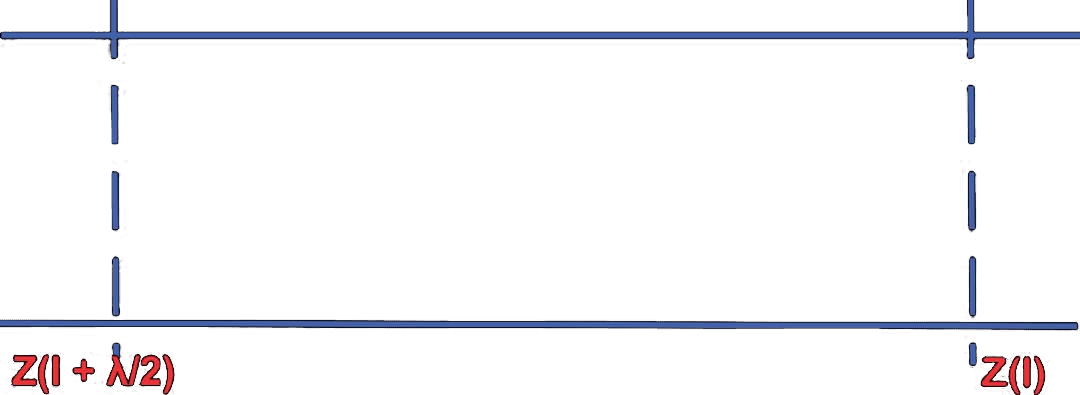
\includegraphics[width=0.8\linewidth]{./graphics/6}
\caption{Z($l$) over distance $\frac{\lambda}{2}$}
\label{fig:astyuif}
\end{figure}

At location ${\left(l+\frac{\lambda}{2}\right)}$, Impedance $= \bar{Z}\left(l+\frac{\lambda}{2}\right)$ substituting ${\left(l+\frac{\lambda}{2}\right)}$ for $l$ in equation~\eqref{eqn:implossless}, we get: 
\begin{align*}
\bar{Z}\left(l+\frac{\lambda}{2}\right) = \left\lbrace \frac{\bar{Z}_L \cos(\beta \left(l+\frac{\lambda}{2}\right)) + j\sin(\beta \left(l+\frac{\lambda}{2}\right))}{\cos(\beta \left(l+\frac{\lambda}{2}\right)) + j\bar{Z}_L \sin(\beta \left(l+\frac{\lambda}{2}\right))}\right\rbrace 
\end{align*}
Since \footnote{$\beta$ represents phase constant}$\beta$ = $ \frac{2\pi}{\lambda}$, therefore,
\begin{dmath*}
\beta\left(l+\frac{\lambda}{2}\right)=\frac{2\pi}{\lambda}\left(l+\frac{\lambda}{2}\right)=\frac{2\pi}{\lambda}l+\pi=\beta l+\pi
\end{dmath*}
\begin{align*}
\bar{Z}\left(l+\frac{\lambda}{2}\right) = \left\lbrace \frac{\bar{Z}_L\cos(\beta l+\pi) + j\sin(\beta l+\pi)}{\cos(\beta l+\pi) + j\bar{Z}_L\sin(\beta l+\pi)}\right\rbrace 
\end{align*}
But 
\[
\cos(\beta l+\pi)=-\cos(\beta l)$ and $\sin(\beta l+\pi)=-\sin(\beta l)
\] 
\begin{dmath*}
\bar{Z}\left(l+\frac{\lambda}{2}\right)=\left\lbrace \frac{-\bar{Z}_L \cos(\beta l) - j\sin(\beta l)}{-\cos(\beta l) - j\bar{Z}_L \sin(\beta l)}\right\rbrace = \left\lbrace \frac{\bar{Z}_L \cos(\beta l) + j\sin(\beta l)}{\cos(\beta l) + j\bar{Z}_L \sin(\beta l)}\right\rbrace\;\;\equiv\bar{Z}(l)
\end{dmath*} 
This is same as original formula obtained for $\bar{Z}(l)$.

Hence $\bar{Z}\left(l+\frac{\lambda}{2}\right)=\bar{Z}(l)$, which proves that impedance repeat itself at $\frac{\lambda}{2}$.

In other words, no matter the length of the transmission line, modulus $\frac{\lambda}{2}$ is  a special information which is available from the impedance relationship.

\subsection{Normalized impedance inverts at every $\frac{\lambda}{4}$ distance}
If we move a distance of $\frac{\lambda}{4}$, we move from a maximum to minimum impedance and vice versa.

At location $l, \textnormal{Impedance}=\bar{Z}(l)$.

Then at location ${(l+\frac{\lambda}{4})}$, Impedance  $=\bar{Z}(l+\frac{\lambda}{4})$. Substituting ${(l+\frac{\lambda}{4})}$ for $l$ in equation~\ref{eqn:implossless}, we get:
\begin{align*}
\bar{Z}\left(l+\frac{\lambda}{4}\right) = \left\lbrace \frac{\bar{Z}(l)\cos(\beta (l+\frac{\lambda}{4})) + jsin(\beta (l+\frac{\lambda}{4}))}{\cos(\beta (l+\frac{\lambda}{4})) + j\bar{Z}(l)\sin(\beta (l+\frac{\lambda}{4}))}\right\rbrace 
\end{align*}
Where 
\begin{dmath*}
\beta(l + \frac{\lambda}{4})=\beta l + \frac{2\pi}{\lambda} \cdot \frac{\lambda}{4} = \beta l + \frac{\pi}{2}
\end{dmath*}
\begin{align*} 
\bar{Z}\left(l+\frac{\lambda}{4}\right) = \left\lbrace \frac{\bar{Z}(l)\cos(\beta l + \frac{\pi}{2}) + j\sin(\beta l + \frac{\pi}{2})}{\cos(\beta l + \frac{\pi}{2}) + j\bar{Z}(l)\sin(\beta l + \frac{\pi}{2})}\right\rbrace
\end{align*}
But $\cos(\beta l + \frac{\pi}{2})= -\sin(\beta l), \sin(\beta l+\frac{\pi}{2})=\cos(\beta l)$
\begin{align*} 
\bar{Z}\left(l+\frac{\lambda}{4}\right) = \left\lbrace \frac{-\bar{Z}(l)\sin(\beta l) + j\cos(\beta l)}{-\sin(\beta l) + j\bar{Z}(l) \cos(\beta l)}\right\rbrace
\end{align*}
\begin{dmath*}
\bar{Z}\left(l+\frac{\lambda}{4}\right) =\frac{j}{j} \left\lbrace \frac{\cos(\beta l) + j\bar{Z}(l)\sin(\beta l)}{\bar{Z}(l)\cos(\beta l) + j\sin(\beta l)}\right\rbrace 
= \frac{1}{\left\lbrace \frac{\bar{Z}(l)\cos(\beta l) + j\sin(\beta l)}{\cos(\beta l) + j\bar{Z}(l)\sin(\beta l)}\right\rbrace} 
=\frac{1}{\bar{Z}(l)}
\end{dmath*}
We can draw an observation that for every $\frac{\lambda}{4}$ distance moved, the normalized impedance inverts itself\footnote{Note the word \textbf{normalized}, it is not absolute impedance}. If absolute impedance is inverted, it is \textbf{admittance}\index{admittance}. The normalized impedance does not have a unit, it is dimensionless. So if I have an impedance greater than $Z_0$ along a transmission line, after $\frac{\lambda}{4}$ distance, it becomes less than $Z_0$ because the normalized impedance is the inverse of the one at previous location. So at $\frac{\lambda}{4}$ distance, impedance inverts after another $\frac{\lambda}{4}$ again it re-inverts becoming the original impedance, which is equivalent to repeating itself at $\frac{\lambda}{2}$ distance. 

Hence, when we talk about the periodicity of the impedance on the transmission line, at $\frac{\lambda}{2}$ the absolute or normalized impedance repeats itself, whereas every distance of $\frac{\lambda}{4}$, the normalized impedance inverts itself. Next on is the study of impedance matching characteristics; this property is used extensively for finding out the impedance transformation which can match impedance on transmission line.

\subsection{The matching condition characteristics}
If the transmission line is terminated by its characteristics impedance, then the impedance seen at every point on the transmission line is equal to the characteristics impedance. So if $Z_L=Z_0$. This implies that $\bar{Z}_L= \frac{Z_L}{Z_0}=1$. Then equation~\eqref{eqn:implossless} becomes:
\begin{dmath*}
\bar{Z}(l) = \left\lbrace\frac{\bar{Z}_L\cos\beta l + j\sin\beta l}{\cos\beta l + j\bar{Z}_L\sin\beta l}\right\rbrace = \left\lbrace \frac{\cos\beta l + j\sin\beta l}{\cos\beta l + jsin\beta l}\right\rbrace = 1
\end{dmath*}
Therefore, irrespective of the length of the transmission line, if the line is terminated in its characteristics impedance, then the impedance seen at every point on the transmission line is equal to the characteristics impedance. This means that once a line is terminated in its characteristics impedance, there is no need to compute the impedance transformation on the line, we can use any length of transmission and the impedance will always be the same along the length of the line. 

$Z_L=Z_0$ i.e when reflection coefficient is zero, there is no reflected wave on the transmission line and we have only forward traveling wave on the transmission line. Forward traveling wave always see an impedance which is equal to the characteristics impedance. This result is not new, it is what we had discussed earlier when we talked about transmission line and that was, if a line is terminated in its characteristic impedance, the impedance seen at every point on the transmission line is equal to the characteristics impedance.

So these are the three very important characteristics of a lossless transmission line.
\begin{enumerate}[(i)]
\item Impedance transformation repeats at every $\frac{\lambda}{2}$ distances.
\item Normalized impedance inverts at every $\frac{\lambda}{4}$ distance.
\item Finally if the line is terminated in its characteristics impedance, the impedance seen at every point of the line is equal to the characteristics impedance.
\end{enumerate}
With this understanding of impedance transformation, now we can go to Power Transfer Calculation of the transmission line.

\section{Power Transfer on Transmission Line}
Initially, our idea was to transfer power from generator to load effectively. In the lossless case, it should be that all generator power is completely transferred to the load. However, we have seen that if the impedance is not equal to the characteristics impedance, then there will always be reflection on the transmission line and whatever energy the generator supplies, part of this energy will get reflected back to the generator. Now when we talk about matching condition\index{matching condition} or maximum power transfer condition\index{matching power transfer condition}, there are two cases to consider;
\begin{enumerate}[(i)]
\item When the power is generated by the generator, it should be maximally transfered to the load.
\item When the reflected power comes back to generator, the generator is not capable of absorbing power, so when the reflected power comes back with a different amplitude and phase, it negatively affects the generator's performance (destructive interference). So it is desirable that the generator should not see any power coming back at it.
\end{enumerate}
For these two reasons that the generator power should be completely delivered to the load and that no reflected power should come back to the generator, we must make sure always that the impedance which the generator sees is always equal to the characteristics impedance. We will study these two issues later but let's study a general case and suppose we have a transmission line which is connected to a generator at  one end and a load at the other end. Then, \emph{how much power will be delivered to the load?} Again using the voltage and current equation, we can write down power at the location of the load i.e power delivered to the load will be given as follows.

At load end, $L=0$ therefore, $e^{-2\beta (l)} = e^{-2\beta (0)}$
\begin{align*}
V(0) &= V^{+} \left\lbrace {1 + \Gamma_L e^{-2\beta(0)}}\right\rbrace\\ 
&= V^{+}\left\lbrace 1 +\Gamma_L \right\rbrace\\
I(0) &= \frac{V^{+}}{Z_0} \left\lbrace{1 - \Gamma_L e^{-2\beta(0)}}\right\rbrace\\ 
&= \frac{V^{+}}{Z_0}\left\lbrace1 -\Gamma_L \right\rbrace
\end{align*}
So from the general voltage and current relationship on the transmission line we have found  out the voltage and current values at load end.

$Z_0$ is real for a lossless line, thus the conjugate of the current equation at the load end is:
\begin{align*}
I^\ast (0) =\frac{V^{+ (\ast )}}{Z_0}\left\lbrace 1 -\Gamma_L \right\rbrace
\end{align*}

Power delivered to load.
\begin{dmath*}
P = \frac{1}{2}\mathfrak{Re}\left\lbrace V(0) I^\ast(0) \right\rbrace= \frac{1}{2}\mathfrak{Re}\left\lbrace V^+(1+\Gamma_L) \times\frac{V^{+(\ast)}}{Z_0} (1-\Gamma_L)\right\rbrace
\end{dmath*}
\begin{equation}
P = \frac{1}{2} \frac{|V^+|^2}{Z_0} \left\lbrace 1 -|\Gamma_L|^2 \right\rbrace\footnotemark
\end{equation}
\footnotetext{
Given $V=a + jb  \quad \quad V^\ast=a-jb$

Then, $V\times V^\ast = (a + jb)(a-jb)= a^2-jab + jab +(jb)(-jb)=a^2 + b^2$

$|V|= \sqrt{a^2 + b^2}$ thus, $|V|^2 = a^2 + b^2$

This implies that $|V|^2 = V \times V^* $}
$\Gamma_L$ is a real value since it is the absolute value taken here.

Recall that,
\begin{align*}\Gamma_L = \frac{ Z_L -Z_0 }{ Z_L + Z_0 }.
\end{align*}

Once load impedance is known, the reflection coefficient at load end is known. Then we can calculate modulus of reflection coefficient so that the power delivered to the load can be calculated if $V^+$ is known. How do we find $V^+ ? $ From the relationship here, if we know the amplitude of the forward traveling wave as well as the load impedance, we can calculate the power from the circuit perspective point of view. We can use a different argument in arriving at the same answer. That is on the transmission line the power supplied from generator, in the form of a traveling wave goes towards the load and we already said that traveling wave always see impedance equal to characteristics impedance. So if the traveling wave has amplitude $V^+$, it is as if this wave is supplying the power to $Z_0$ in the lossless case. So one can say now that  a wave having amplitude $V^+$ going forward direction sees impedance $Z_0$.

Power carried by forward wave:  
\begin{align*}
P_{\textnormal{for}} = \frac{1}{2} \frac{{|V|^+}^2}{Z_0}
\end{align*}
When this gets to the load, part of the energy will get reflected back, and this backward traveling wave has amplitude $V^-$ which also sees characteristics impedance.

The power carried by this wave:
\begin{align*}
P_{\textnormal{ref}} = \frac{1}{2}\frac{{|V^-|}^2}{Z_0}
\end{align*}
which is the power reflected by load in the backward wave.

Therefore,
\begin{align*} 
\textnormal{Power delivered to load}, P\\
=& \textnormal{Power transferred to load}\\
&- \textnormal{Power reflected}\\
=& \frac{1}{2} \frac{{|V^+|}^2}{Z_0} -\frac{1}{2} \frac{{|V^-|}^2 }{Z_0}\\
=& \frac{1}{2} \left\lbrace \frac{{|V^+| }^2}{Z_0} -\frac{ {|V^-|}^2 }{Z_0} \right\rbrace\\
=& \frac{1}{2} \frac{{|V^+|}^2}{Z_0} \left\lbrace 1 - {
\begin{vmatrix}
\frac{V^-}{V^+}
\end{vmatrix}^2}\right\rbrace
\end{align*}
Recall that $\Gamma_L =\frac{V^-}{V^+}$.
\begin{align*}
P_L=\frac{1}{2} \frac{{|V^+|}^2}{Z_0} \left\lbrace 1 - { \Gamma_L }^2 \right\rbrace.
\end{align*}
So when we compute the power transfer on a transmission line, it is either done using circuit theory concept or wave theory concept. Thus we have found the real part i.e the power actually supplied to the load. One then asks \emph{how do we calculate for complex part or put differently, how do we compute the complex power at any location on the transmission line?}. 

If we calculate the power flow along any point on the transmission line not necessarily at the load end, what will that indicate? To test that theory, let's get the voltage and current at any arbitrary location on the transmission line i.e
\begin{align*} 
V(l) = V^+ e^{j\beta l} \left\lbrace 1 + \Gamma_L e^{-j2\beta l} \right\rbrace,\\ 
I(l) = \frac{V^+}{Z_0} e^{j\beta l} \left\lbrace 1 - \Gamma_L e^{-j2\beta l} \right\rbrace
\end{align*}
Complex Power at location $l$ is thus given as:
\begin{dmath*}
P(l) = \frac{1}{2} (V I^\ast) 
= \frac{1}{2} \left(V^+ e^{j\beta l} \left\lbrace 1 + \Gamma_L e^{-j2\beta l} \right\rbrace \right) \times \left(\frac{V^+}{Z_0} e^{-j\beta l} \left\lbrace 1 - \Gamma_L e^{j2\beta l} \right\rbrace\right)
=\frac{1}{2} \frac{{|V^+|}^2}{Z_0} \left( 1 + \Gamma_L e^{-j2\beta l}\right)\left(1 - \Gamma e^{j2\beta l}\right)
= \frac{1}{2} \frac{{|V^+|}^2}{Z_0}\left(1 - \Gamma_L e^{j2\beta l} + \Gamma_L e^{-j2\beta l} - {|\Gamma_L|^2}\right)
=\frac{1}{2} \frac{{|V^+|}^2}{Z_0}\left\lbrace 1 - {|\Gamma_L|}^2 - \Gamma_L \left(e^{j2\beta l} - e^{-j2\beta l}\right)\right\rbrace
\end{dmath*}
Recall, \( \jmath2\sin\theta = {e}^{\jmath\theta} - {e}^{\jmath\theta}\), so,
\begin{dmath} 
P(l) = \frac{1}{2} \frac{{|V^+|}^2}{Z_0}\left\lbrace 1 - {|\Gamma_L|}^2 - j2\Gamma_L \sin(2\beta l)\right\rbrace
= \frac{1}{2} \frac{{|V^+|}^2}{Z_0}\left\lbrace 1 - {|\Gamma_L|}^2 - \mathfrak{Im}\lbrace\Gamma_L{e}^{-j2\beta l}\rbrace\right\rbrace
\end{dmath}
Thus, given the complex power, the real part is $1 - {|\Gamma_L}|^2$ which is the resistive power, and the imaginary part is $ j2\Gamma_L \sin(2\beta l) = \mathfrak{Im}\lbrace\Gamma_L{e}^{-j2\beta l}\rbrace$ which is the reactive power.

Therefore, at any location of the transmission line, the power is complex, the interesting thing to note is that the resistive power at any point is equal to the power which we earlier calculated that is delivered to the load end. So for a lossless line the resistive power at any point along the line is the same as the power which is delivered to the load\footnote{
This can be explained with the line of throught that the resistive power finally gets to the load if the line is lossless, since there is no absorption of power at any point along the line and so all the resistive power gets to the load because the load is the part where you have resistive component and power can be  absorbed in that location.
}. Hence at any point on the transmission line, power transfer of the resistive part is completely delivered to the load and as such the resistive power which is the actual power flow should be independent of any location on the line.

However the reactive power is a function of $l$, which shows the energy stored at different location along the transmission line. Now we have two parts when we calculate the power on a transmission line. \emph{There is a resistive power which is a measure of power flow which ultimately gets delivered to the load and the reactive power which measures the amount energy storage at different location along the line and depends on the value of voltage and current at that location.} Recall that the voltage and current equations are standing waves and thus the energy stored also varies at different location along the transmission line. Therefore, in conclusion, the reactive power will vary at different locations across the line while the resistive power which is the power delivered to the load will be independent of location of the transmission line.
\begin{exmp}
\subsubsection*{Power Flow on a Lossless Line}
A generator with voltage $V_g = 300\angle0^o$V and internal resistance, $Z_g = 50\varOmega$ is connected to a load, $Z_L = 75\varOmega$ through a 50-$\varOmega$ lossless transmission line of length $l = 0.15\lambda$.
\begin{enumerate}[(a)]
\item Compute the input impedance of the line at the generator, $Z_{in}$.
\item Compute the time-average power delivered to the line, $P_{in}$.
\item Compute the time-average power delivered to the load, $P_L$. How does $P_{in}$ compare to $P_L$? Explain.
\end{enumerate}

\subsubsection*{Solution}
\begin{figure}[h]
\centering
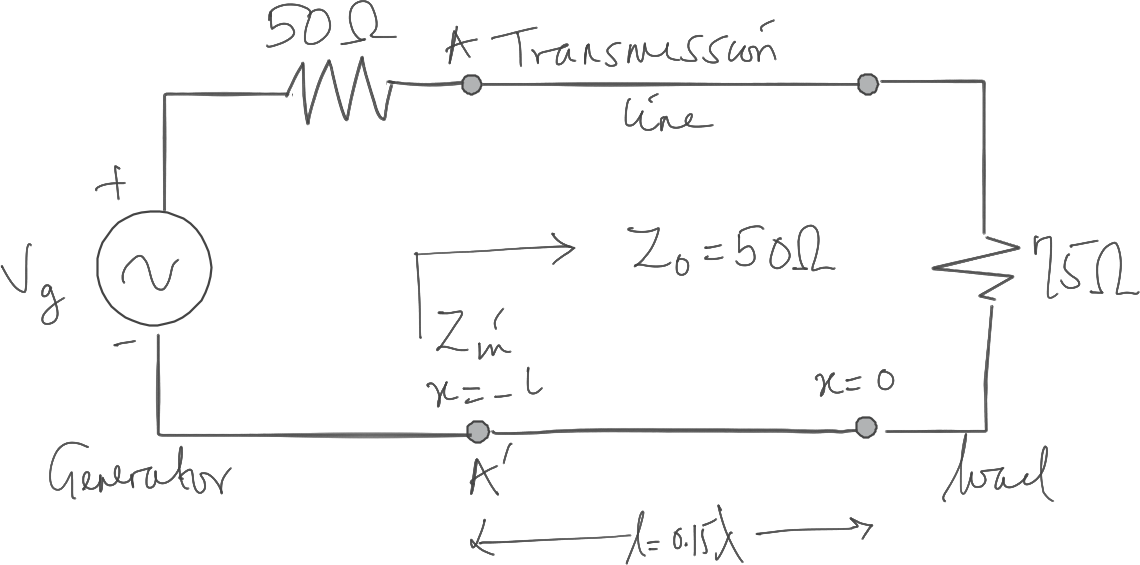
\includegraphics[width=1\linewidth]{./graphics/power_problem_temp}
\caption{Circuit Diagram of Worked example}
\label{fig:powerproblem}
\end{figure}
\begin{figure}[h]
\centering
\includegraphics[width=.7\linewidth]{./graphics/power_problem2_temp}
\caption{Transformed Circuit Diagram of Worked example}
\label{fig:powerproblem2}
\end{figure}

From the transmission line shown in figure~\ref{fig:powerproblem}, to find $Z_{in}$ we will use the impedance transformation relation in equation~\eqref{eqn:implossless} such that
\begin{dmath*}
Z_{in} = Z_0\left[\frac{Z_L\cos\beta l + jZ_0\sin\beta l}{Z_0\cos\beta l + jZ_L\sin\beta l} \right]
= 50\left[\frac{75\cos(0.3\pi) + j50\sin(0.3\pi)}{50\cos(0.3\pi) + j75\cos(0.3\pi)} \right]\footnotemark
= (41.25 - j16.35)\varOmega
\end{dmath*}
\footnotetext{
$\beta l = \frac{2\pi}{\lambda}\times 0.15\lambda = 0.3\pi$
}
The time-average power delivered to the line is the power at point AA' in figure~\ref{fig:powerproblem} which is given as
\begin{dmath*}
P_{in} = \frac{1}{2}\mathfrak{Re}\left\lbrace V_{in}I_{in}^*\right\rbrace
\end{dmath*}
The voltage and current at point AA' can be found using the voltage and current variations in a lossless transmission line from equations~\eqref{eqn:voltagefromloadlossless} and~\eqref{eqn:currentfromloadlossless} but $|V^+|$ is not known. Instead we turn to some circuit laws and analyze the transformed circuit shown in figure~\ref{fig:powerproblem2}\footnote{This approach will be dealt with appropriately in \autoref{sec:evalvplus}}.

Thus we can determine $V_{in}$ and $I_{in}$ from the circuit diagram is figure~\ref{fig:powerproblem2} as
\begin{align*}
I_{in} &= \frac{V_g}{Z_g + Z_{in}} 
= \frac{300\angle0^o}{50 + (41.25 - j16.35)}\\
&= 3.24\angle10.16^oA\\
V_{in} &= I_{in}Z_{in} = 3.24\angle10.16^o(41.25 - j16.35)\\
&= 143.6\angle-11.46^oV
\end{align*}

Thus, the power delivered to the line is
\begin{dmath*}
P_{in} = \frac{1}{2}\mathfrak{Re}\lbrace V_{in}I_{in}^\ast\rbrace
= \frac{1}{2}\mathfrak{Re}\lbrace 143.6\angle-11.46^o\times3.24\angle-10.16^o\rbrace
=\frac{143.6\times3.24}{2}\cos(21.62^o)
= 216W
\end{dmath*}

Now, let us determine the power delivered to the load end, $P_L$, given as
\begin{dmath*}
P_L = \frac{1}{2}\mathfrak{Re}\lbrace V_L I_L^\ast\rbrace
\end{dmath*}
\emph{How do we determine $V_L$ and $I_L$?} We can determine $V_L$ and $I_L$ using equations~\eqref{eqn:voltagefromloadlossless} and~\eqref{eqn:currentfromloadlossless} where $l = 0$ such that we get
\begin{align*}
V(0) &= V_L = V^+\lbrace1 + \Gamma_L\rbrace\\
I(0) &= I_L = \frac{V^+}{Z_0}\lbrace1 + \Gamma_L\rbrace
\end{align*}
So we need to evaluate $V^+$ using the same voltage equation but with $l = L = 0.15\lambda$, that is
\begin{align*}
V_{in} &= V^+e^{j\beta l}\lbrace1 + \Gamma_Le^{-2j\beta l}\rbrace\\
V^+ &= \frac{V_{in}}{e^{j\beta l}\left(1+\left(\dfrac{Z_L - Z_0}{Z_L + Z_0}\right)e^{-2j\beta l}\right)}\\
&=\frac{\dfrac{143.6\angle-11.46^o}{e^{j0.3}}}{1+\left(\dfrac{75 - 50}{75 + 50}\right)e^{-j0.6\pi}}\\
&= \frac{\dfrac{143.6\angle-11.46^o}{e^{j0.3}}}{1+0.2e^{-j0.6\pi}}\\
&= 150\angle-54^oV
\end{align*}
Thus the values for $V_L$ and $I_L$ are
\begin{align*}
V_L &= V^+\lbrace1 + \Gamma_L\rbrace = 150\angle-54^o(1 + 0.2)\\
&= 180\angle-54^o V\\
I_L &= \frac{V^+}{Z_0}\lbrace1 + \Gamma_L\rbrace = \frac{150\angle-54^o}{50}(1 - 0.2)\\
&= 2.4\angle-54^oA
\end{align*}

Now we determine the power delivered to the load which is
\begin{dmath*}
P_L = \frac{1}{2}\mathfrak{Re}\lbrace V_L I_L^\ast\rbrace
= \frac{1}{2}\mathfrak{Re}\lbrace 180\angle-54^o\times 2.4\angle54^o\rbrace
= 216W
\end{dmath*}

We can see that $P_{in} = P_L$ as expected because the line is lossless so the input power should equal the delivered power at the load point.
\end{exmp}

\section{Evaluation of $\mathbf{V^{+}}$}\label{sec:evalvplus}
So far, our transmission line analysis (voltage and current equations, impedance transformation, power transfer analysis and so on) has been derived in terms of $V^+$. $V^+$ is a final arbitrary constant in the solution of the differential equation of transmission line that we are yet to evaluate. It is the amplitude of the incident voltage, which we have assumed in known a priori. Now the question is \emph{how do we evaluate $V^{+}$?}.

Considering the circuit in figure~\ref{fig:qwerrtt}, $Z_L$ is transformed to $Z^{'}_L$, from position BB' to AA'. $Z^{'}_L$ is the impedance of the load as seen by the generator end. With $Z_L$ transformed to $Z^{'}_L$, the whole circuit is reduced to a lump circuit as shown in figure~\ref{fig:qwerrtt}.
\begin{figure}[h]
\centering
\includegraphics[width=0.7\linewidth]{./graphics/qwerrtt fixed}
\caption{Transformation of load impedance from $Z_L$ to $Z_{L}^'$}
\label{fig:qwerrtt}
\end{figure}

Considering the lumped circuit, the voltage and current equations are\footnote{
The voltage and current relations take the limit as the size of the circuit tends to zero so it is valid for any arbitrary frequency.
}
\begin{align}
V_A &= \frac{Z^'_L}{Z^{'}_L + Z_s} . V_s\label{eqn:transimpvoltage}\\
I_A &= \frac{V_A}{Z^{'}_L}\label{eqn:transimpcurrent}
\end{align} 
We can then determine the voltage and current at the tranformed location using the transmission line equations, such that,
\begin{align*} 
V_A &= V(l) = V^+ e^{j\beta l} \left\lbrace 1 + \Gamma_L e^{-j2\beta l} \right\rbrace\\
I_A &= I(l) = \frac{V^+}{Z_0} e^{j\beta l} \left\lbrace 1 - \Gamma_L e^{-j2\beta l} \right\rbrace
\end{align*}
So we know now the value of $V_A$ and $I_A$ from the lumped element side of view and the transmission line element side of view. We can equate the two to get,
\begin{equation} 
V_A = \frac{Z^{'}_L}{Z^{'}_L + Z_s} . V_s = V^+ e^{j\beta l} \left\lbrace 1 + \Gamma_L e^{-j2\beta l} \right\rbrace\label{eqn:evaluatev+voltage}
\end{equation}
\begin{equation}
I_A = \frac{V_A}{Z^{'}_L} = I(l) = \frac{V^+}{Z_0} e^{j\beta l} \left\lbrace 1 - \Gamma_L e^{-j2\beta l} \right\rbrace
\label{eqn:evaluatev+current}
\end{equation}
So solving equation~\ref{eqn:evaluatev+current} making $V^{+}$ the subject of the formula, we get the expression of $V^+$ as follows. 
\begin{equation} 
V^+ = \frac{Z^{'}_L V_s e^{-j\beta l}}{(Z_S + Z^{'}_L)(1 + \Gamma_L e^{-j2\beta l })}, 
\end{equation}
$\alpha, \beta, l, \Gamma_L$ and $Z_0$ are all known values, so now we have a known value for $V^+$.

From here $V^+$ can be determined and then substituted into the power equation and so power delivered to the load can be calculated or power at any point along the line. This is a complete solution to voltage and current on the transmission line.

\subsection*{Summary}
Table~\ref{tab:transparams} show the transmission line parameters for lossless and low-loss conditions that have been discussed and derived.
\begin{table}[h]
\caption[short]{Transmission line parameters for lossless and low-loss conditions}
\label{tab:transparams}
\begin{tabular}{l c l}
{\bf Lossless}&   	$\leftrightarrow$  & {\bf Low-loss}  \\ 
$\alpha$ = 0 &  & $\alpha = \dfrac{1}{2}R\sqrt{\frac{C}{L}} + \dfrac{1}{2}G\sqrt{\frac{C}{L}}$\\
$\beta = \omega\sqrt{LC}$ & & $\beta = \omega\sqrt{LC}$\\
$\gamma = j\beta$ & & $\gamma = \alpha + j\beta$\\
$Z_0 = \sqrt{\frac{L}{C}}$ = real &  & 	$Z_0 = \sqrt{\frac{L}{C}}\left(1 - j\frac{R}{2\omega L} - j\frac{G}{2\omega C}\right)$
\end{tabular} 
\end{table} 

Other parameters that are derived are as follows and they apply equally to lossless and low-loss conditions.
\begin{align*}
\Gamma_L = \frac{Z_L - Z_0}{Z_L + Z_0} = \frac{\bar{Z_L} - 1}{\bar{Z_L} + 1} = \frac{V^-}{V^+}
\end{align*}
\begin{align*}
\text{VSWR, }\rho = \frac{1 + |\Gamma_L|}{1 - |\Gamma_L|}
\end{align*}
\begin{align*}
R_\max &= Z_0 \left( \frac{1 + |\Gamma_L|}{1 - |\Gamma_L|}\right) = Z_0 \rho\\
Z_\max &= \frac{|V_\max|}{|I_\min|}
\end{align*}
\begin{align*}
R_\min &= Z_0 \left(\frac{1 - |\Gamma_L|}{1 + |\Gamma_L|}\right) = \frac{Z_0}{\rho}\\
Z_\min &= \frac{|V_\min|}{|I_\max|}
\end{align*}

For Impedance transformation, we have
\begin{align*}
Z(l) &= Z_0\left\lbrace\frac{Z_L\cos\beta l + jZ_0\sin\beta l}{jZ_0\sin\beta l + Z_L\cos\beta l}\right\rbrace\\ 
&= Z_0\left\lbrace\frac{Z_L\cosh\gamma l + Z_0\sinh\gamma l}{Z_0\cosh\gamma l + Z_L\sinh\gamma l}\right\rbrace
\end{align*}

Lastly, the power flow equations
\begin{dmath*}
P_L = \frac{1}{2}\frac{|V^+|}{Z_0}\lbrace 1 - |\Gamma_L|^2\rbrace\quad\text{Real power}
\end{dmath*}
\begin{dmath*}
P(l) = \frac{1}{2}\frac{|V^+|}{Z_0}\lbrace 1 - |\Gamma_L|^2\rbrace - \mathfrak{Im}\lbrace \Gamma_L e^{- j2\beta l}\rbrace\quad\text{Complex power}
\end{dmath*}
\[
V^+ = \frac{Z_L^{'}V_s e^{-j\beta l}}{(Z_s + Z_L^{'})(1 + \Gamma_L e^{-j2\beta l})}
\]

\section*{Exercises}
\begin{ExerciseList}
\Exercise[label={ex61}]
A 50$\Omega$ lossless transmission line is connected to a load of $50 + j50\Omega$. The maximum voltage measured on the line is 50V. Find the power delivered to the load and the peak voltage at the load end of the line.
\begin{figure}[h]
\centering
\includegraphics[width=1\linewidth]{./graphics/antenna_power_problem}
\caption{Antenna configuration for Ex.~\ref{ex62}}
\label{fig:antennapowerproblem}
\end{figure}
\Answer[ref={ex61}]
(a) $P_L = 9.55W$ (b) $|V_L| = 30.9$V

\Exercise[label={ex62}]
If the two-antenna configuration shown in figure~\ref{fig:antennapowerproblem} is connected to a generator with $V_g = 250\angle0^o$ and internal resistance $Z_g = 50\varOmega$, how much average power is delivered to each antenna?
\Answer[ref={ex62}]
Power delivered to each antenna is 76.68W
\end{ExerciseList}
%\chapter{\textbf{Introduction to Smith Chart}}
\section{Introduction}
In the previous lectures, we were able to derive equations for different parameters for a transmission line such as;
\begin{enumerate}[(i)]
\item 	Power delivered to the load
\item	Voltage standing wave ratio (VSWR)
\item	Voltage and current maximum and minimum
\item	Reflection coefficient
\item	Impedance transformation ratio etc.
\end{enumerate}

Up till now, we analyze transmission line characteristics using analytical methods. But in this lecture, we utilize another approach for analyzing the problems of a transmission line which is the \textbf{Graphical Approach}.
This approach involves solving the problems of a transmission line from an image called a \textbf{Smith Chart}.
This approach is most preferred for solving transmission line problems than the analytical approach owing to the following reasons;\\
\begin{enumerate}[(i)]
\item Images have a much longer-lasting impression than equations or text on the human mind.
\item	It is much simpler to use in solving transmission line problems compared to the analytical approach owing to the fact that calculations can be reduced to a significant amount when analyzing the problems of the transmission line.
\item	It is a very compact way of representing the impedance characteristics of transmission lines.

This method if properly understood makes solving transmission line problems much easier and faster.  It can also be used as a means of cross-checking the solution obtained using the analytical method so that one does not go conceptually wrong in solving transmission line problems.
It is very important to understand that the graphical approach does not give the voltage and current solutions but rather it gives the following parameters:
\begin{enumerate}[(i)]
\item	Impedance transformation relationship 
\item Reflection coefficient
\item Voltage standing wave ratio (VSWR)
\item Location of voltage minimum
\item	Location of voltage maximum etc.
\end{enumerate}
\end{enumerate}

This lecture simply develops a basic framework for analyzing the transmission line by graphical approach.
\begin{figure}[h]
\centering
\includegraphics[width=0.5\linewidth]{./graphics/mjhdj}
\caption{Complex Z Plane}
\label{fig:mjhdj}
\end{figure}

\section{Plane Transformation}
It was established in previous lectures that impedances possess a real part and a complex part and this can be written as;
\begin{equation*}
Z= R+jX
\end{equation*}
Where R  represents the real part called Resistance and $jX$ represents the complex part called Reactance. When using the graphical approach, the absolute impedance is not required but instead, normalized impedance is used. It therefore means that, given any impedance, it must be normalized with respect to the characteristic impedance (Zo). i.e
\begin{equation*}
\bar{Z}=\frac{Z_L}{Z_o}
\end{equation*}
where $\bar{Z}$ = normalised impedance\\
$Z_o$ = characteristic impedance\\
$Z_L$   =  absolute  impedance \\
Normalizing the equation above we have: 
\begin{equation*}
\bar{Z}= r + jx
\end{equation*}
Let us represent this expression graphically on a plane which we shall call the impedance plane or Z-plane for short.
\begin{figure}[h]
\center\includegraphics[width=0.5\linewidth]{./graphics/TransLine2}
\label{fig:transline2}
\end{figure}

From the figure~\ref{fig:transline2}, it is seen that the resistance r is always real and positive whereas the reactance could be positive which represents Inductive Reactance or negative which represents Capacitive Reactance.\\
Figure~\ref{fig:transline2} represents a possible load which can be obtained from the z-plane.  It can be deduced that all point on the imaginary axis plus all points on the right half plane covers all possible passive loads of a transmission line.
Graphically, the statement is represented in the figure~\ref{fig:oigvbnkliu}
\begin{figure}[h]
\centering
\includegraphics[width=0.6\linewidth]{./graphics/oigvbnkliu}
\caption{All Possible Passive Load}
\label{fig:oigvbnkliu}
\end{figure}

Solving problems of transmission lines using the Z-plane is quite difficult. For this reason, the impedance which was normalized with respect to the characteristic impedance is transformed into another plane which we shall call the Complex Co-efficient Plane or the Gamma Plane ($ \Gamma $).\\ Doing this, expresses the impedances in a form which makes the calculation much simpler.
The transformation from the Z plane to the $ \Gamma $ plane is made possible due to the one-to-one relationship that exists between the impedance Z and the reflection co-efficient $ \Gamma $ i.e
\begin{equation*}
\Gamma = \frac{Z_L - Z_o}{Z_L + Z_o}
\end{equation*}
Normalizing we have
\begin{equation*}
\Gamma= \frac{\bar{Z} - 1}{\bar{Z} + 1}
\end{equation*}\\ or
\begin{equation*}
\bar{Z}= \frac{1 + \Gamma}{1 - \Gamma}
\end{equation*}
This expression simply means if the normalized impedance is known, we can find the reflection coefficient and vice versa.It also means for every value of impedance Z, there is a corresponding value of reflection co-efficient $ \Gamma\ $.\\
Just as Z has real and imaginary parts, $ \Gamma\ $ also has real and imaginary parts which can be written in either rectangular form\\
i.e. $ \Gamma = u + Jv$ or polar form	$\Gamma$ = $Re^{j\theta}$

From previous chapters, it was established that the reflection coefficient for all passive loads is always less than or equal to one($ \Gamma\ \leq 1).$\\
At an open or short circuit, reflection co-efficient $ \Gamma\ $ = 1; for any other impedance $ \Gamma\  < 1$.  So by plotting the reflection co-efficient($ \Gamma\ $) we have the right half Z plane mapping into a unit circle in the gamma plane as shown in figure below.
\begin{figure}[h]
\centering
\includegraphics[width=0.7\linewidth]{./graphics/oiuhgvcx}
\caption{Z Plane and Complex $\gamma$ plane}
\label{fig:oiuhgvcx}
\end{figure}

In summary, when solving graphically the problems of transmission lines, the basic idea is to take the impedance which is normalized with respect to the characteristics impedance and do a transformation of this impedance into the gamma plane.

\section{Circle of Constant Resistance and Reactance}
It was established that since there is a one-to-one transformation between the Z plane and $\Gamma$ plane every point on the Z plane is mapped to a point on the $ \Gamma$ plane. In this section, we will be mapping the impedance from the Z plane to the gamma plane.\\
Recall,
$ \bar{Z}= r + jx $ and also
\begin{equation}
\bar{Z}= \frac{1 + \Gamma}{1 - \Gamma}
\end{equation}
\begin{equation}
r + jx =\frac{1 + \Gamma}{1 - \Gamma}
\end{equation}
\begin{equation}
\Gamma\ = u + jv
\end{equation}
substituting 7.3 in 7.2 we have:
\begin{equation}
r + jx = \frac{(1 + u) + jv}{(1 - u) -jv}
\end{equation}
conjugating 7.4 we have:
\begin{equation*}
r + jx = \frac{(1 + u) + jv}{(1 - u) -jv}\times \frac{(1 - u) + jv}{(1 - u) +jv}
\end{equation*}
expanding the expression, we have:
\begin{equation*}
r + jx =\frac{1 - u^2 + jv(1 + u) + jv(1 - u) - v^2}{(1 - u)^2 + jv(1 - u) - jv(1 - u) + v^2} 
\end{equation*}
simplifying the expression, we have:
\begin{equation*}
r + jx = \frac{1 - u^2 + 2jv - v^2}{(1 -u)^2 + v^2}
\end{equation*}
re-arranging the expression
\begin{equation*}
r + jx = \frac{1 - (u^2 + v^2) + 2jv}{(1 - u)^2 + v^2}
\end{equation*}
separating the real and imaginary parts, we have:
\begin{equation}
r = \frac{1 - (u^2 + v^2)}{(1 - u)^2 + v^2}
\end{equation}
and
\begin{equation}
x = \frac{2v}{(1 - u)^2 + v^2}
\end{equation}
considering the real part :	
\begin{equation*}
r = \frac{1 - (u^2 + v^2)}{(1 - u)^2 + v^2}
\end{equation*}
\begin{equation*}
r((1 - u)^2 + v^2) = 1 -(u^2 + v^2)
\end{equation*}
\begin{equation*}
r - 2ur + u^2r + v^2r = 1 - u^2 - v^2
\end{equation*}
collecting like terms, we have:
\begin{equation*}
u^2(r + 1) -2ur + (r - 1) + v^2(r + 1) = 0
\end{equation*}
dividing through by r + 1:
\begin{equation}
u^2 - 2u(\frac{r}{r + 1}) + v^2 +(\frac{r - 1}{r + 1}) = 0
\end{equation}
by using the method of completing the squares:
\begin{align*}
(u - \frac{r}{r+1})^2\;\;+\;\;v^2\;\;+\;\;(\frac{r-1}{r+1})\;\; - \;\;(\frac{r}{r+1})^2\;\; = \;\;0
\end{align*}
\begin{equation*}
(u - \frac{r}{r + 1})^2 + v^2 =(\frac{r}{r + 1})^2 -(\frac{r - 1}{r + 1}) 
\end{equation*}
\begin{equation*}
(u - \frac{r}{r + 1})^2+ v^2 =\frac{r^2 -(r^2 -1)}{(r + 1)^2}
\end{equation*}
\begin{equation}
(u - \frac{r}{r + 1})^2+ v^2 = \frac{1}{(r + 1)^2}
\end{equation}
the expression obtained above represents the equation of a circle in the uv plane centered at$ (\frac{r}{r + 1}, 0) $ with radius $ (\frac{1}{r + 1}) $

equation 7.8 can be compared  with  the equation of a circle of radius r, with origin at x = a and y = 0 which is $ (x - a)^2 + y^2 = r^2 $\\ 
considering the imaginary part, we have:
\begin{equation*}
x =\frac{2v}{(1 - u)^2 + v^2}
\end{equation*}
\begin{equation*}
x(1 - 2u + u^2 + v^2) = 2v
\end{equation*}
\begin{equation*}
v^2x - 2v + u^2x - 2ux + x = 0
\end{equation*}
divide through by x
\begin{equation*}
v^2 - \frac{2v}{x} +u^2 - 2u + 1 = 0
\end{equation*}
factorising the expresssion becomes:
\begin{equation*}
(u - 1)^2 -1 + (v - \frac{1}{x})^2 -\frac{1}{x^2} + 1 = 0
\end{equation*}
\begin{equation}
(u - 1)^2 + (v - \frac{1}{x})^2 = \frac{1}{x^2}
\end{equation}
equation~\eqref{eqn:circleuvplane} represents the equation of a circle in the UV plane centred at $ (1,\frac{1}{x}) $ with radius $ (\frac{1}{x}) $.
It can also be compared with the equation of a circle centered at (a,b) and radius r which is $ (x - a)^2 + (y-b)^2 = r^2 $

From the two expressions obtained from solving for r and x,  It can be deduced that for any value of r and x, we gets a circle on the gamma plane. The circle that corresponds to r is called the Circle of Constant Resistance while that corresponds to x is called the Circle of Constant Reactance.

All points on the circle of constant resistance have the same resistance value in the Z plane and all points on the circle of constant reactance will have the same reactance in the Z plane.

\section{Circle of Constant Resistance}
This circle  obtained from the real point of normalized impedance $ \bar{Z} $, the circle lies on the real axis in the gamma plane, and its radius varies from 0 to $\infty$. Plotting the circle for different values of r, we have as shown above;
\begin{figure}[h]
\centering
\includegraphics[width=0.5\linewidth]{./graphics/ouytre}
\caption{Circle of Constant Rsistance}
\label{fig:ouytre}
\end{figure}

\begin{equation*}
u^2 - 2u\left(\frac{r}{r + 1}\right) + v^2 +\left(\frac{r - 1}{r + 1}\right) = 0
\end{equation*}
Center = $(\frac{r}{r + 1},0)$ and radius = $\frac{1}{r + 1}$\\\\
Lets plot for various value of r, by varying it from zero to infinity, with r = 0, Center (0,0), and radius = 1.\\
At $r = 1$ which means $Z = Z_o$ we get the centre as $(\dfrac{1}{2}, 0)$ and radius as $\dfrac{1}{2}$.\\
The figure above shows that as the value of r increases, the centre shifts towards the right and the radius keeps reducing towards zero. At $r = \infty$, the centre is (1,0) and the radius is zero, which is denoted as a dot on the real axis. Hence for increasing r, we have the following set of curves.\\\\
\begin{figure}[h]
\centering
\includegraphics[width=0.5\linewidth]{./graphics/rghmgfcx}
\caption{Circle of Increasing Resistance}
\label{fig:rghmgfcx}
\end{figure}
We observe that all circle of the constant resistance circles passes through u = 1, and v = 0\\
Complex $\Gamma$ plane, Constant x circle where center is $(1,\frac{1}{x})$, and radius = $\frac{1}{x}$\\
For $x = \infty,Center = (1,0), radius = 0$\\
$x = 1,Center = (1,1), radius = 1$\\
$x = 2,Center = (1,\frac{1}{2}), radius = \frac{1}{2}$\\
\section{Circle of Constant Reactance}
\begin{align*}
u^2+v^2-2u\left(\frac{2}{x}\right)v+1=0
\end{align*}\\
Center = $(1,\frac{1}{x})$ and radius = $\frac{1}{x}$. \\
The centre of this circle lies on a vertical plane passing through the real axis at u=1 and the radius varies from $-\infty$ to $+\infty$.\\\\
From the plot above, it can be deduced that the centre always lie on a line u = 1 and v = 0. As x increases, the centre comes down along u = 1 line and the radius decreases.  
From the two plots above it is seen that both circles of constant resistance and reactance pass through co-ordinate (u,v) = (1,0). This signifies the uniqueness of the points.  When these two circles are superimposed, we have figure it as shown in figure~\ref{fig:uytrdbn}.
\begin{figure}[h]
\centering
\includegraphics[width=0.5\linewidth]{./graphics/uytrdbn}
\caption{Two Set of Circles Superimposed}
\label{fig:uytrdbn}
\end{figure}

we observe that all circles of constant reactance also pass through (u,v) = (1,0). So the (u,v) = (1,0) is a special point as both constant resistance and reactance circle passes through that point. For the constant reactance circle, x = 0 gives the center $(1,\infty)$ and radius $\infty$. 

In this lecture, we are not concerned with reflection co-efficients that are greater than one, we are only interested in reflection co-efficient that are less than or equal to 1 which is represented by a unit circle of radius = 1. It therefore means that any other point outside this range of reflection co-efficient ($\Gamma$) is not of practical relevance to us since it does not represent a passive load.  Although, the constant reactance circle fills the entire space, but only the portion that satisfies $ \Gamma\ \leq 1$ is practically useful to us and this lies within the unit circle of the complex gamma plane.
\begin{figure}[h]
\centering
\includegraphics[width=0.5\linewidth]{./graphics/ijnbvcxw}
\caption{Two Set of Circles Superimposed}
\label{fig:ijnbvcxw}
\end{figure}
\begin{figure}[h]
\centering
\includegraphics[width=0.5\linewidth]{./graphics/sddfghj}
\caption{Useful part of the Two Superimposed Circles}
\label{fig:sddfghj}
\end{figure}

This figure above is a superposition of constant resistance and reactance circles so, we can now identify the impedance point on the gamma plane.  The outermost circle of radius, $r= 1$, is called the limit circle for the gamma plane for which $\Gamma\ \leq 1$.\\

\section{Characteristics of the set of Circle}
\begin{enumerate}[(i)]
\item All constant resistance circles have their centre lying on the positive axis and complex gamma plane.
\item All the circles passes through the point u=1, v = 0
\item As the value of r increases, the centre shift towards the right from the origin to point u = 1 and the radius decreases.
\item The constant reactance circle has a vertical line passing through u=1 and the upper half represents the positive reactance and the lower half negative reactance.
\item As the reactance value increases, the centre of the circle approaches the u-axis, the radius of the circle decreases and the size of the circle reduces.
\item When x = $\infty$, the size of the circle = 0  and this  becomes just a point at (u,v) = (1,0).
\end{enumerate}

The superposition of the two circles is now a coordinate system for impedance on the complex gamma plane. This is called the \textbf{Smith Chart}.  This will be elaborated on in  the next section.
\section{The Smith Chart}
\begin{figure}[h]
\centering
\includegraphics[width=0.7\linewidth]{"./graphics/smith_chart (2)"}
\caption{A Complete Smith Chart}
\label{fig:smithchart-2}
\end{figure}

\footnote{\includegraphics[scale=0.09]{./graphics/a21}PHILIP HAGAR SMITH (April 29, 1905 - August 29, 1987) was an electrical engineer who became famous for his invention of the SMITH CHART. He graduated from Tufts College in 1928 with a BS degree in electrical engineering while working for Bell Telephone Laboratories. He invented his eponymous smith chart during the period of being faced with the challenge of how to show and evaluate multiple complex impedance parameters which can range from zero to infinity. When asked why he invented the chart, Smith explained \textquotedblleft From the time I could operate a slide rule, I've been interested in graphical representations of mathematical relationship\textquotedblright. This interest in representing mathematical relationships in graphical form is what led to the invention of the smith chart.}

The smith chart is a graphical aid designed for electrical and electronics engineers to assist in solving problems of the transmission lines and matching circuits. It is a product of superimposing the circle of constant resistance and the circle of constant reactance. It can be used to simultaneously display multiple parameters such as the impedances, admittances, reflection co-efficient e.t.c.
It is plotted on the complex reflection co-efficient plane in two dimensions and is scaled in normalized impedance (which is most common), normalized admittance or both. It has circumstantial scaling of wavelengths and degrees. The wavelengths scale is used in distributed component problems and represents the distance measured along the transmission line connected between the generator and the load to the point under consideration.
Let us mark out some important points on the simplified smith chart below.
\begin{figure}[h]
\centering
\includegraphics[width=0.5\linewidth]{"./graphics/473 drawingjhgfd"}
\caption{A Simplified Smith Chart}
\label{fig:473-drawingjhgfd}
\end{figure}

\begin{enumerate}[(i)]
\item The point A or any other point lying on the outermost circle correspond to r = 0 while any point lying on the horizontal axis represents x = 0
\item The intersection of this horizontal axis and the outermost circle corresponds to r = 0,x = 0 at A which corresponds to a load that is short circuited from the impedance point of the line. It therefore means that point A is a short circuit.
\item At point B where the two set of circles degenerate into, corresponds to $r=\infty$ and $x=\infty$ which is nothing but an open circuit.\item Any point between A and B on the outermost circle represents pure reactance. Above the u axis inside the limit circle , we have the inductive loads while below the u axis in the limit circle we have the capacitive load( it therefore means we can tell what kind of load we have by where it lies on the smith chart).
\item At point C where r = 0 and x = +1, corresponds to purely inductive reactance whose magnitude is equal to the characteristic impedance of the line.
\item At point D where r = -1 and x = -1 represents a purely capacitive reactance whose magnitude is equal to the characteristic impedance of the line.
\item The centre of the limit circle has one more special point M which is the origin, it is the intersection of r = 1 circle and x = 0 line.

At M the impedance equal to the characteristic impedance of the line and that is the point of greatest interest to us because that point represents the matched condition of the transmission line.
\end{enumerate}
These points if properly understood can be used to solve transmission line problems with ease.

To solve transmission line problems using the smith chart, it should be held such that the most clustered portion of the circle should be held with the right hand of the user because the real axis at the complex gamma plane is in that direction and the complex imaginary plane is in the vertical direction.

With this understanding,
\begin{enumerate}[(i)]
\item Calculation on conversion from the complex reflection co-efficient plane to the impedance plane and vice versa can be done easily.
\item Impedance points on the smith chart can be marked and used to find co-ordinates of the point which gives the reflection co-efficient easily.
\end{enumerate}
The smith chart is a handy tool for solving very complex impedance transformation problems.

%\section{Concept of constant VSWR circle in lossless transmission line analysis}\label{lec:lec8}
Previously, we developed a graphical tool by transforming the complex impedance of a transmission line into the gamma plane called the Smith chart. This we have seen as the superimposition of circles of constant resistance on the circles of constant reactance masked within the limit circle $|\Gamma| \leq 1$. Before we go into the use of the Smith chart for transmission line calculations, we develop one more set of circles called the constant VSWR circles and then superimpose it on the Smith chart.

We know that:
\begin{equation*}
\Gamma(l) =\Gamma_L e^{-j2\beta{l}}
\end{equation*}
Where $l$ is the distance from the load point towards the generator, $\Gamma_{L}$ is the voltage reflection coefficient at the load end and $\beta$ is the phase constant of the transmission line. The voltage reflection coefficient, $\Gamma_L$ can be expressed in polar form as $|\Gamma_{L}|e^{j\theta_L}$ such that
\begin{equation*}
\Gamma{(l)} = |\Gamma_{L}|e^{j\theta_L}\cdot e^{-j2\beta l}
\end{equation*}
Where $\theta_L$ is the phase angle of deflection of the load.
\begin{equation}
\Gamma{(l)} =|\Gamma_L|e^{j(\theta_L - 2\beta{l})}
\end{equation}
The total phase becomes $\theta_L - 2\beta{l}$. Hence the reflection coefficient $\Gamma{(l)}$ has magnitude $|\Gamma_L|$ on the complex gamma plane but a phase angle that varies with distance from the load end. Since $l$ is positive when moving towards the generator, therefore, the phase increases in the negative direction. The distance of the point $|\Gamma_L|$ from the centre of the circle remains constant but its angle changes with respect to $l$. Hence $|\Gamma_L|e^{j(\theta_L - 2\beta l)}$ represents a \emph{constant VSWR circle}\index{constant vswr circle} having the same centre of origin with that of the complex gamma plane as shown in figure~\ref{fig:lkjhgryn}.

When moving towards the generator with increasing length, $l$, a corresponding anti-clockwise rotation in the gamma plane is experienced. That is on this circle, the magnitude of the reflection coefficient is the same no matter what point, but the angle differs and we know that,
\begin{equation}
VSWR, \rho = \frac{1 + |\Gamma_L|}{1 - |\Gamma_L|}
\end{equation}
\begin{figure}[h]
\centering
\includegraphics[width=0.7\linewidth]{\pathtopartone/graphics/lkjhgryn}
\caption{Constant VSWR Circle}
\label{fig:lkjhgryn}
\end{figure}

Since $|\Gamma_L|$ is the same at any point on the circle, then the VSWR is the same for all points on the circle, hence we call the circle a constant VSWR circle. 
% Note that while solving transmission line problems, we have to draw constant VSWR circles on the Smith chart so the Smith chart readily gives the constant resistance and reactance circles in the limit circle of $|\Gamma_L|\leq 1$.
One should always note that the centre of all VSWR circles is the same as that of the origin of the complex gamma plane and the magnitude of the reflection coefficient is always less or equal to 1. A larger radius of $|\Gamma_L|$ gives more reflection coefficient with a lower impedance match and a smaller radius of $|\Gamma_L|$ gives a smaller magnitude of reflection coefficient and a better impedance match (see figure~\ref{fig:poiuyfd}).

When we say that we have better impedance matching on the Smith chart, visually speaking, we mean that the point closest to the centre of the Smith chart is better for impedance matching because it represents a smaller magnitude of the reflection coefficient. 

With the understanding of superimposing the constant VSWR circle on the Smith chart, we can therefore solve the transmission line problem.
\begin{figure}[h]
\centering
\includegraphics[width=0.57\linewidth]{\pathtopartone/graphics/poiuyfd}
\caption{Impedance matching with different constant VSWR circles}
\label{fig:poiuyfd}
\end{figure}

\section{Transmission Line Analysis using Admittance}
However, as we have said, you may have connections in transmission lines that are in the form of parallel connections and we know that from circuit analysis, anywhere we have parallel connections, it is easier to deal with admittances rather than impedances. Before now, we have been discussing load impedances and load characteristics impedance of transmission lines. However, if we have to make parallel connections on the transmission line, we represent the load as admittances and characteristics admittance before we carry out the analysis on the Smith chart. 

Thus, in this section, we will determine how the Smith chart is used when we compute in terms of admittances. Since the Smith chart gives the normalized impedances of the transmission line, the same thing will be derived for admittances so we shall first define the normalized admittance of the transmission line and for that, we would require what is called the \emph{characteristic admittance}\index{characteristics admittance} of the line. The characteristic admittance is given in equation~\eqref{eqn:characteristicsadmit}
\begin{equation}
Y_0 = \frac{1}{Z_0}\label{eqn:characteristicsadmit}
\end{equation}
Then, normalizing the admittance would yield
\begin{align*}
\bar{Y} = \frac{Y}{Y_0}\quad\text{thus, load admittance is }\quad\bar{Y}_L = \frac{Y_L}{Y_0}
\end{align*}
The reflection co-efficient as derived in equation~\eqref{eqn:refcoefficientfromload07} is given as
\begin{equation*}
\Gamma = \frac{Z - Z_0}{Z + Z_0} 
\end{equation*}
To determine the reflection coefficient in terms of admittance we replace the impedance $Z$ and characteristics impedance are then expressed as the inverse of admittance $\frac{1}{Y}$ and inverse of the characteristics admittance $\frac{1}{Y_0}$ respectively.
\begin{equation*}
\Gamma = \frac{\frac{1}{Y} - \frac{1}{Y_0}}{\frac{1}{Y} + \frac{1}{Y_0}}
\end{equation*}
We further simplify as follows;
\begin{dmath*}
\Gamma = \frac{Y_0 - Y}{Y_0 + Y}
= \frac{1 - \frac{Y}{Y_0}}{1 + \frac{Y}{Y_0}}
= \frac{1 - \bar{Y}}{1 + \bar{Y}} = -1\cdot\left(\frac{\bar{Y} - 1}{\bar{Y} + 1}\right)
\end{dmath*}
The negative sign indicates a phase change of 180\textdegree\footnote{
As -1 is a phase change of $\pi, e^{j\pi} = \cos\pi + j\sin\pi = -1$
} thus, it can be expressed as
\begin{equation}
\Gamma = \frac{\bar{Y} - 1}{\bar{Y} + 1}e^{j\pi}
\end{equation}
So the reflection coefficient written in terms of normalized admittances is the same as the reflection coefficient written in terms of normalized impedance except for the 180\textdegree\; phase change.

This implies that the same value is derived for the reflection coefficient when calculated using the normalized impedance or admittance except there is a phase shift of 180\textdegree\; that would be experienced on the transmission line. In other words, on the complex gamma plane of the Smith chart, the 180\textdegree\; phase shift will correspond to a rotation of 180\textdegree\; (see figure~\ref{fig:zstyuiou}). Essentially, the normalized impedance and admittance can be calculated in the same way except when carrying out calculations for normalized admittances, there is a rotation of 180\textdegree\; on the complex gamma plane otherwise, all other values and parameters remain unchanged.
\begin{figure}[h]
\centering
\includegraphics[width=0.6\linewidth]{\pathtopartone/graphics/zstyuiou}
\caption{Impedance equivalent of Admittance on the gamma plane}
\label{fig:zstyuiou}
\end{figure}

Hence as far as the constant VSWR circles are concerned, any point on the Smith chart rotated by 180\textdegree\; corresponds to the normalized admittance with corresponding circles of constant resistance and circles of constant reactance. 

\emph{What would be the complex representation of the admittance?}
\begin{dmath*}
\bar{Y}=\frac{G + jB}{Y_0} = g + jb
= \text{conductance} + j (\text{susceptance})
\end{dmath*}
If we interchange $r$ with $g$ and $x$ with $b$, then the circles through the point on the constant VSWR circle will be the \textbf{circle of constant conductance} and the \textbf{circle of constant susceptance} which are similar to the circle of constant resistance and circle of constant reactance except that they are rotated by 180\textdegree\;. This implies that our analysis with admittances will resemble one where every point on the Smith chart is flipped and so the clustered end goes to the left-hand side as shown in figure~\ref{fig:invertedsmithchart}.
\begin{figure}[h]
\centering
\includegraphics*[width=0.7\linewidth]{\pathtopartone/graphics/inverted_smith_chart}
\caption{Inverted Smith chart}\label{fig:invertedsmithchart}
\end{figure}

Alternatively, we can keep the Smith chart orientation the same and rotate the complex gamma axis by 180\textdegree\; before doing calculations for admittances. So, if we develop an understanding that we will not rotate the Smith chart, that means we want to use it in its original form, that is, the most clustered part of it to our right, then if we do the impedance calculations, the positive real axis is towards right and the positive imaginary axis goes up. However, during calculations using the Smith chart unchanged for admittances, the positive real axis is towards the left and the positive imaginary axis will be downwards. Normally, whenever we do the Smith chart calculations, we do not rotate the Smith chart. For the impedance, the gamma axis is the positive top right plane and for admittances, the bottom left plane is the positive plane. Depending on whether we are calculating for the impedance or admittances and if we require fixed measurement in the complex gamma plane, then the axis has to be rotated appropriately by 180\textdegree\; depending on whether we are using the impedance or admittance. This is important when finding the phase of the reflection coefficient, otherwise, the axis of the gamma plane is insignificant. So without worrying about the axis of the complex gamma plane, we can use the same Smith chart for the admittance as well as the impedance calculations. This is the reason why when you look at the Smith chart carefully, you will see that the upper half of the Smith chart is denoted by $(x,b)$ and the lower part $(-x,-b)$. The circles are denoted by either $r$ or $g$ so any normalized value of $r$ is equal to the same normalized value of $g$ which represents the same circle. 

Hence, as long we are dealing with a normalized quantity, the impedance and admittance can be treated exactly the same way on the Smith chart. However, the normalized values of $g$ and $r$ or $b$ and $x$ have different meanings physically. But do they represent the same physical conditions? The answer is NO! For example, $r = 0; x = 0$, corresponds to a short circuit condition\textemdash\;the impedance is zero\textemdash\;however, if we take a normalized value of admittance with $g=0, b=0$ which represents admittance equal to zero, it is not a short circuit but an open circuit condition on the line. Therefore, the normalized values of impedances and admittances can be treated exactly the same way in calculations but not the same interpretations for the physical conditions. In summary, mathematically, $g = 0\quad, b = 0\Longrightarrow$ open circuit and $g = \infty, b = \infty \Longrightarrow$ short circuit. 
\begin{figure}[h]
\centering
\includegraphics[width=1\linewidth]{\pathtopartone/graphics/jnbkvfld}
\caption{Physical variation of impedance and admittance}
\label{fig:jnbkvfld}
\end{figure}

Let us, therefore, consider the points on the Smith chart for the admittance where the special points $r$ and $x$ are replaced with $b$ and $g$ respectively. Maintaining the original orientation of the Smith chart then for the admittance Smith chart, the upper half of the Smith chart represents capacitive loads and the lower half represents the inductive loads (see figure~\ref{fig:jnbkvfld}). With these in mind, the use of the Smith chart for impedance or admittance calculation is very straightforward.

Now let us make use of the Smith chart to solve transmission line problems. 

\section{Use of Smith chart for Transmission Line Calculation}
Let us consider the simplest problem we can think of for the transmission line. Suppose for a given load, we want to find the reflection coefficient at the load point. Analytically, we can use the formula $\frac{Z_L - Z_0}{Z_L + Z_0}$ but in using the Smith chart, the problem is much simpler to solve. Remember the impedance and admittance you have on the Smith chart are all normalized quantities. So we take the following steps

\subsection*{Procedure:}
\begin{enumerate}[(i)]
\item Normalize $Z_{L}$ to get $\bar{Z}_{L}$, that is, $\frac{Z_{L}}{Z_{0}}$.
\item Determine this point on the Smith chart, that is, $r+jx$ by identifying the constant resistance and reactance circle with the value $r$ and $x$ respectively and the point of intersection (see figure~\ref{fig:lfds}).
\begin{figure}[h]
\centering
\includegraphics[width=0.7\linewidth]{\pathtopartone/graphics/lfds}
\caption{Point of intersection of circles of constant resistance and reactance}
\label{fig:lfds}
\end{figure}

\item Determine the distance of the point of intersection from the origin to find the magnitude of the reflection coefficient, $|\Gamma_L|$ and then the corresponding phase is given as $\theta_L$.
\end{enumerate}

So without doing any calculation, just by measuring its distance, and the angle, we get the magnitude of reflection coefficient, $|\Gamma_L|$
and phase angle, $\theta_L$. 

Similarly, for the admittance, let $\bar{Y} = g + jb$. We determine the point of intersection on the Smith chart the same way as that of impedance, however, to find out the complex reflection coefficient, maintaining the orientation, then the positive real axis is to the left. So the phase angle will be measured from the positive real axis as shown in figure~\ref{fig:kjhgfds}. We summarize the steps as follows.
\begin{figure}[h]
\centering
\includegraphics[width=0.7\linewidth]{\pathtopartone/graphics/KJHGFDS}
\caption{Determining the reflection coefficient for admittance on a Smith chart}
\label{fig:kjhgfds}
\end{figure}

\subsection*{Procedure:}
\begin{enumerate}[(i)]
\item Normalize the admittance $\bar{Y}$ with the characteristic admittance, $Y_0$.
\item Determine the point on the Smith chart which is the point of intersection of the circle of constant conductance, $g$ and the circle of constant susceptance, $b$.
\item Determine the distance of the point from the origin to find the magnitude of the reflection coefficient, $|\Gamma_L|$ but the phase angle, $\theta_L$ will be measured from the positive real axis (see figure~\ref{fig:kjhgfds}). 
\end{enumerate}

Thus, when we are using normalized impedance or admittance, the appropriate rotation has to be made on the coordinate axes of the Smith chart. Once this is done, the calculation of the complex reflection coefficient is very straightforward. Mark the normalized points on the Smith chart. Find the distance from the origin to the marked point and then measure the angle from this marked point from the positive real axis which differs for impedance and admittance while maintaining the orientation of the Smith chart. 

In another simple transmission line problem, let us suppose the magnitude of the reflection coefficient and phase angle is given, but we need to find the load. The steps are summarized below.
\subsection*{Procedure:}
\begin{enumerate}[(i)]
\item Draw a circle of radius equal to the magnitude of the reflection coefficient from the origin.
\item Determine phase angle from the positive real axis depending on whether the impedance or admittance value at the load is required.
\item Mark the point on the circle and find the corresponding $r$ and $x$ circles or $g$ and $b$ circles.
\item Multiply the normalized impedance or admittance by the characteristic impedance or admittance to get the load impedance or admittance.
\end{enumerate}

\subsection{Impedance Transformation}
A common problem in transmission lines is impedance transformation. We have shown how it is done analytically but \emph{how can we perform impedance transformation graphically?} 
\begin{figure}[h]
\centering
\includegraphics[width=0.7\linewidth]{\pathtopartone/graphics/wertuyuk}
\caption{Tranformed impedance at distance $l$ from the load}
\label{fig:wertuyuk}
\end{figure}

If the load impedance is given as shown in figure~\ref{fig:wertuyuk} and we are asked to find the reflection coefficient and load impedance at another point $l$ on the transmission line, that is, given $Z_L$ or $Y_L$, we are to find $Z_L$ or $Y_L$ at distance $l$ from the load. We will use a hypothetical sketch of the Smith chart shown in figure~\ref{fig:uytrewsxcvbj}.
\begin{figure}[h]
\centering
\includegraphics[width=0.9\linewidth]{\pathtopartone/graphics/uytrewsxcvbj}
\caption{Points along the constant r and x Circles}
\label{fig:uytrewsxcvbj}
\end{figure}

\subsection*{Procedure:}
\begin{enumerate}[(i)]
\item If the impedance is not normalized, we normalize all impedances.
\item Determine the point, $\bar{Z}_L$, on the Smith chart and draw a circle passing through the point from the origin. As we have seen earlier, the magnitude of the reflection coefficient remains the same as the point moves on the circle which is a constant VSWR circle.
\item Determine the point that translates to a distance $l$. In a Smith chart, one rotation, $2\pi$ translate to a phase change of $2\beta{l}$\footnote{
As we move along the transmission line, the phase angle changes by $2\beta{l}$ in the clockwise direction (from load towards generator).
}, that is $2\beta{l} = 2\pi\Longrightarrow l = \frac{\pi}{\beta} = \frac{\lambda}{2}$\footnote{
$\beta = \frac{2\pi}{\lambda}$
} (see figure~\ref{fig:mjhtre}). Therefore, a full rotation around the Smith chart corresponds to a distance of $\frac{\lambda}{2}$ on a constant VSWR circle\footnote{
The above analysis makes sense since one characteristic of the transmission line is that its impedance characteristics repeat every $\frac{\lambda}{2}$ distance on the line.
}. So we determine the corresponding $x\lambda$ for the value of $l$ moving clockwise along the VSWR from the point $\bar{Z}_L$.
\begin{figure}[h]
\centering
\includegraphics[width=0.7\linewidth]{\pathtopartone/graphics/mjhtre}
\caption{Tranformed impedance at distance $l$ from the load}
\label{fig:mjhtre}
\end{figure}

\item Mark the new point on the Smith chart and determine the magnitude of the reflection coefficient and phase angle as shown in figure~\ref{fig:uyhbgjvkclxse} or the circle of constant resistance and circle of constant reactance to determine the normalized impedance at $l$, that is, $\bar{Z}_{l} = r + jx$.
\begin{figure}[h]
\centering
\includegraphics[width=0.7\linewidth]{\pathtopartone/graphics/uyhbgjvkclxse}
\caption{New phase angle after rotation}
\label{fig:uyhbgjvkclxse}
\end{figure}

\item Multiply the normalized impedance at $l$ by the characteristic impedance $Z_0$ to get $\bar{Z}_{l}$ at the new location.
\end{enumerate}

A more general overview of a transmission problem is one where the impedance is given at a particular location and we need to transform the impedance to another location. If the new location is to the left of the previous impedance (towards the generator) then we follow the aforementioned steps, otherwise, we reverse the direction of the angular rotation instead of $-2\beta{l}$, we have $+2\beta{l}$ which is counter-clockwise rotation. Hence, moving towards the generator will be a clockwise rotation and moving away from the generator will be an anti-clockwise rotation. The sense of rotation in impedance calculations is extremely important because that tells us whether to move toward the generator or away from the generator. Therefore, in all transmission line calculations, the direction of the generator should be given much consideration because that will decide the movement along the transmission line.

For admittance calculations, the same steps apply except in the sense of the position of the positive real axis (see figure~\ref{fig:dfyui}).
\begin{figure}[h]
\centering
\includegraphics[width=0.7\linewidth]{\pathtopartone/graphics/dfyui}
\caption{Phase angle measurement with admittance Smith chart}
\label{fig:dfyui}
\end{figure}

Analytically, the impedance transformation requires the calculation of sine and cosine functions that are unusually very complicated. With the help of the Smith chart, impedance transformation is easily achieved.

\subsection{Voltage Standing Wave Ratio (VSWR)}
Another quantity that is a measure of reflection is the VSWR and we established previously that $R_\max = Z_0\rho$ and $R_\min = \frac{Z_0}{\rho}$. If we normalize $R_\max$ and $R_\min$ then we get:
\begin{equation}
\bar{R}_\max = r_\max = {\rho}
\end{equation}
and
\begin{equation}
\bar{R}_\min = r_\min = \frac{1}{\rho}
\end{equation}
Therefore, the maximum normalized resistance, $r_\max$ gives the VSWR, $\rho$. Similarly, on the left side of the VSWR circle on the Smith chart, we have $r_\min$. Hence $r_\min = \frac{1}{\rho}$. Thus, \emph{how do we determine the VSWR graphically?} On the real axis, we have only resistance and no reactance so points of intersection of the constant VSWR circle with the real axis give the maximum and minimum normalized resistance (see figure~\ref{fig:oijhgfdsa}). The reason why we call it the constant VSWR circle is that as determined in equation~\eqref{eqn:vswr}, it is given as $\frac{1 + |\Gamma|}{1 - |\Gamma|}$ which is constant for a lossless transmission line and these values of $r_\max$ and $r_\min$ can easily be deduced from the VSWR circles without a need to calculate. The VSWR is taken as the ratio of maximum impedance on the line to characteristics impedance.
\begin{figure}[h]
\centering
\includegraphics[width=0.7\linewidth]{\pathtopartone/graphics/oijhgfdsa}
\caption{Maximum and Minimum Points of Resistance}
\label{fig:oijhgfdsa}
\end{figure}

Hence, the maximum value of the normalized resistance gives VSWR. The maximum value of resistance in terms of normalized quantity is seen when the VSWR circle intersects the real axis on the right side. The rightmost side corresponds to the impedance which is $r_\max$ and the reactance for that is zero\textemdash\;$r_\max$ is nothing but $\rho$. Similarly, the minimum value which we see on the transmission line is $r_\min = \frac{1}{\rho}$. The minimum resistance which corresponds to the leftmost intercept on the real axis gives $\frac{1}{\rho}$. Thus once the load impedance or any other impedance is marked on the Smith chart and the constant VSWR circle is drawn, the calculation of the VSWR is straightforward same as the reflection coefficient and transformed/normalized impedance. It is just a matter of plotting and reading different values on a Smith chart.

Next is to find out the locations of the minimum and maximum voltage and current on the transmission line. 

\subsection{Location of the minimum and maximum voltage and current}
Suppose we want to find out the distance of current or voltage maximum at the load end of the transmission line. From our knowledge of transmission line, at the point of maximum voltage, we experience minimum current which gives $R_\max$ then at minimum voltage, we experience maximum current which gives $R_\min$ hence $R_\max$ corresponds to $V_\max$, $I_\min$ and $R_\min$ corresponds to $V_\min$, $I_\max$. To find out these locations from the load, we move from point, $Z_L$ to $r_\max$ and $r_\min$ as shown in figure~\ref{fig:lkjtresx}. The corresponding clockwise angles, $\theta_\max$ and $\theta_\min$, covered indicate the distances $l_\max$ and $l_\min$ towards the generator.
\begin{figure}[h]
\centering
\includegraphics[width=0.7\linewidth]{\pathtopartone/graphics/lkjtresx}
\caption{Location of the maximum and minimum values of voltage and current}
\label{fig:lkjtresx}
\end{figure}

We compute the corresponding distances $l_\max$ and $l_\min$, 
recall that $2\beta{l} = \theta\Longrightarrow l =\frac{\theta}{2\beta}$. Hence,
\begin{align*}
l_\max = \frac{\theta_\max}{2\beta}\quad\text{and}\quad l_\min = \frac{\theta_\min}{2\beta}
\end{align*}
These give the distances from the load point. From figure~\ref{fig:lkjtresx}, $\theta_\max < 180^o(\pi)$ and $270^o\left(\frac{3\pi}{2}\right) <\theta_\min >360^o(2\pi)$ and they, therefore, are the angles that are moved to get from load to $r_\max$ and $r_\min$ respectively.

More generally,
\begin{dmath}
l = \frac{\theta_\min}{2\beta}
=\frac{\theta_\max + \pi}{2\beta} 
= \frac{\theta_\max}{2\beta} + \frac{\lambda}{4}
\end{dmath}

\begin{exmp}\label{exmp:locatepoints}
\subsubsection*{Locate the points on the Smith chart}
Locate the following points on the Smith chart (Take characteristic impedance, $Z_{0}$ = 50$\Omega$).

\begin{enumerate}[(a)]
\item 50+j75$\varOmega$
\item 10+j0$\varOmega$
\item 0-j80$\varOmega$
\item $\Gamma=0.3\angle60^o$
\item VSWR, $\rho=2.5$
\item $R_\min$ on $\rho$ = 1.5 circle
\end{enumerate}

\subsubsection*{Solution}
All impedances seen on the Smith chart are normalized impedances. Therefore, for impedance (a), (b), and (c), we will first normalize these points with the characteristic impedance such that
\begin{align*}
\bar{A}&=\frac{A}{Z_{0}}
=\frac{50 + j75}{50}\\
&=1+j1.5\\
\bar{B}&=\frac{B}{Z_{0}}
= \frac{10 + j0}{50}\\
&=0.2+j0\\
\bar{C}&=\frac{C}{Z_{0}}
= \frac{0 - j80}{50}\\
&=0-j1.6
\end{align*}

To locate point A on the Smith chart, we first identify the constant resistance circle of $r = 1.0$. It is the circle that passes through the centre of the Smith chart from the right-hand side (see figure~\ref{fig:workedexample1}). Next, we identify the constant reactance circle of $x = 1.5$. Recall that the circles above the real axis passing through the centre are the inductive reactance, while the circles below the line are the capacitive reactance. Since the value $x = 1.5$ is positive, it should be the constant inductive reactance circle. The point of intersection of these circles represents the normalized impedance, A, $1 + j1.5$. The same steps apply when identifying points B and C on the Smith chart.
\begin{figure}[h]
\centering
\includegraphics[width=1\linewidth]{\pathtopartone/graphics/"Smith chart"}
\caption{Worked Example}
\label{fig:workedexample1}
\end{figure}

To locate the point in (d) which is the reflection coefficient, the approach is quite different. First, we measure the length of the diameter of the constant resistance circle $r = 1.0$ and record its value. In our case, we measured $7.6cm$. Thus we can determine the radius of a reflection coefficient of magnitude, $0.3$, that is, by multiplying the length, $7.cm$ with the value of the reflection coefficient which is $0.3$, we will get a value, $2.28cm$. 

Next, we draw a circle of radius $2.28cm$ from the origin on the Smith chart (see figure~\ref{fig:workedexample1}). Note that the degree of rotation (circumference of the gamma plane\textemdash limit circle) is calibrated in both degrees and distance. To locate the corresponding phase, we look along the circumference showing \textquotedblleft ANGLE OF REFLECTION COEFFICIENT IN DEGREES\textquotedblright\; we will locate the angle 60\textdegree\; anticlockwise. Then draw a straight line through the centre of the plane to the located angle 60\textdegree\; on the Smith chart. The point of intersection of the circle and the line is the point, $\Gamma = 0.3\angle60^o$ on the Smith chart (see figure~\ref{fig:workedexample1}).

To locate the point in (e), which is the VSWR of value 2.5, we will locate the point that reads $r = 2.5$ along the real axis on the Smith chart and draw a circle passing through that point from the origin. The VSWR circle of 2.5 is drawn through that point.

To locate the point in (f), first, we draw the VSWR circle of value 1.5 using the steps discussed above. The rightmost side along the circle where the real axis intersects the VSWR circle is the normalized $R_\max$ or $r_\max$ and the leftmost side is the normalized $R_\min$ or $r_\min$. Therefore we record the value at the leftmost side and multiply the value by the characteristic impedance
\begin{align*}
r_\min &= \bar{R}_\min = \frac{R_\min}{Z_0}\\
R_\min &= \frac{r_\min}{Z_0} = 0.75 \times 50\\
&= 37.5\Omega
\end{align*}
\end{exmp}

\section*{Exercises}
\begin{ExerciseList}
\Exercise[label={ex81}] Locate the following points on the Smith chart for a 70-$\varOmega$ high frequency lossless line.
\begin{enumerate}[(a)]
\item 140 + j91$\varOmega$
\item $\Gamma=0.5\angle29^o$
\item $R_\max$ on $\rho = 3$ circle
\end{enumerate}
\Answer[ref={ex81}]
solution for exercise~\ref{ex81}
\end{ExerciseList}
%\begin{exmp}
\subsubsection*{Transmission line analysis using a Smith chart}
A 50$\Omega$ line is terminated in a load impedance $25+j35\Omega$. Find the following using a Smith chart.
\begin{enumerate}[(a)]
\item Reflection coefficient in cartesian and polar form,
\item Reflection coefficient and impedance at a distance of $0.2\lambda$ from the load end of the line.
\item VSWR on the line.
\end{enumerate}

\subsubsection*{Solution}
We are given $Z_{L}=25+j35\varOmega$ and $Z_{0}=50\varOmega$, so first, we normalize the load impedance
\begin{dmath*}
\bar{Z_{L}}=\frac{25+j35}{50}=0.5+j0.7
\end{dmath*}
We mark this point on the Smith chart as shown in figure~\ref{fig:workedexample2}.
\begin{figure}[h]
\centering
\includegraphics[width=1\linewidth]{\pathtopartone/graphics/"Smith chart 1"}
\caption{Worked Example}
\label{fig:workedexample2}
\end{figure}

To get the reflection coefficient, we draw a circle from the origin of the Smith chart through the marked point (normalized load impedance), A. The distance between point A and the centre gives the magnitude of the reflection coefficient. \footnote{
The distance is read from the scale for reflection coefficient E or I at the bottom of the Smith chart page

\underline{Note}: This method is different from that used in example~\ref{exmp:locatepoints} and both methods are correct
}. We read the value as;
\begin{align*}
|\Gamma_{L}| = 0.52
\end{align*}

To determine the angle $\phi_{L}$, we draw a straight line from the origin through point A to the outermost circle as shown in figure~\ref{fig:workedexample2}. From the scale that reads \textquotedblleft ANGLE OF REFLECTION COEFFICIENT\textquotedblright\;, read the angle the line makes from the positive real axis. The value gives the angle of the reflection coefficient in polar form so that the reflection coefficient at the load is $0.52\angle100^o$ in polar form.

The cartesian form is obtained by converting the polar form to the cartesian form as shown below
\begin{align*}
\Gamma_{L} &= 0.52\angle100^o\\
&= 0.52e^{j100}\\
&= 0.52{\cos100 + j\sin100}\\
&= -0.09+j0.512
\end{align*}

The next step is to get the reflection coefficient at a distance of $0.2\lambda$ from the load point, that is, $\Gamma(0.2\lambda)$. 

First, we identify the scale on the outermost circle that reads \textquotedblleft WAVELENGTHS TOWARDS GENERATOR\textquotedblright\; and measure the value measured at point A which we obtained as $0.11\lambda$. To move a distance $0.2\lambda$ towards the generator means to move clockwise along the scale\footnote{
Similarly, moving towards the load on the Smith chart means to move in the anticlockwise direction along the scale that reads \textquotedblleft WAVELENGTHS TOWARDS LOAD\textquotedblright\;.
}. We mark this point as "B", which has the value $0.11\lambda + 0.2\lambda=0.31\lambda$. We draw a straight line through the origin of the Smith chart and point B and determine the point of intersection with the VSWR circle. The point is marked "P" (see figure~\ref{fig:workedexample2}) which is the point of the reflection coefficient moved $0.2\lambda$ towards the generator. 

Recall the magnitude of the reflection coefficient is given by the distance between the centre of the smith chart and the point "P". And the angle is measured from the positive real axis. We read the value as
\begin{align*}
\Gamma(0.2\lambda) = 0.52\angle316^o
\end{align*}

To find the normalized impedance at point P, we locate the constant resistance and reactance circles through the point. In our case we obtained
\begin{align*}
\bar{Z_L}=1.4-j1.37\\
\text{Thus, }Z_L &=Z_{0}\times\bar{Z_L}\\
&= 50(1.4-j1.37)\\
&= 70-j68.5\varOmega
\end{align*}

Next, we obtain the value $\rho$ by reading the value at the rightmost side of the VSWR circle (see figure~\ref{fig:workedexample2}).
\begin{align*}
VSWR, \rho = 3.8
\end{align*}
\end{exmp}

\begin{exmp}
\subsubsection*{Transmission line analysis with Admittances}
A line is terminated in a normalized admittance of $\bar{Y_{L}}$ =  $0.2-j0.5\varOmega$. Find;
\begin{enumerate}[(a)]
\item The location of the maximum voltage from the load end. 
\item The reflection coefficient, normalized admittance and normalized impedance at a distance $0.12\lambda$ from the load.
\end{enumerate}

\subsubsection*{Solution}
Now, in this problem, we are dealing with admittances instead of impedances. The admittance we are given here is already normalized, so we mark the point, $\bar{Y_L} = 0.2 - j0.5$, on the Smith chart as shown in figure~\ref{fig:workedexample3}.
\begin{figure}[h]
\centering
\includegraphics[width=1\linewidth]{\pathtopartone/graphics/"smith chart 3"}
\caption{Worked Example}
\label{fig:workedexample3}
\end{figure}

Next, we draw a circle from the origin of the Smith chart through that point $\bar{Y}_L$ which should help us determine the position of maximum voltage, reflection coefficient, normalized admittance and normalized impedance at $0.12\lambda$ from the load.

\subsubsection*{(a) Location of the voltage maximum from the load end}
For the admittance Smith chart, the maximum voltage will now lie on the leftmost side of the VSWR circle of the Smith chart. This point is marked as $V_\max$ on the Smith chart (see figure~\ref{fig:workedexample3}). The distance between $\bar{Y}_L$ and $V_\max$ on the Smith chart is the location of the maximum voltage, moving towards the generator. \footnote{
Recall we move clockwise when moving towards the generator.
}.

\subsubsection*{(b) Reflection coefficient, normalized admittance and impedance at a distance $0.12\lambda$ from the load}
First, we note the distance corresponding to $\bar{Y}_L$ which we measured as $0.424\lambda$ on the Smith chart. Moving a distance of $0.12\lambda$ towards the generator implies that the new location is $0.424\lambda + 0.12\lambda = 0.544\lambda$. But the highest value on the wavelength scale is $0.5\lambda$ so the value on the scale which corresponds to $0.544\lambda$ is $0.044\lambda$\footnote{
$0.544\lambda-0.5\lambda$
}. Next, we draw a line from the origin of the Smith chart through that point and mark the point of intersection of the line with the VSWR circle as $\bar{Y}$ (see figure~\ref{fig:workedexample3}). We read the corresponding value of normalized admittance as:
\begin{align*}
\bar{Y} = 0.18 + j0.28\Omega
\end{align*}

To get the normalized impedance at the distance of $0.12\lambda$ from the load point, we transform the admittance by $\frac{\lambda}{4}$\footnote{
Recall that the normalized impedance inverts itself every $\frac{\lambda}{4}$
}. Put differently, the normalized admittance is the reciprocal(inverse) of the normalized impedance. A transformation by $\frac{\lambda}{4}$ can easily be calculated on the Smith chart by drawing a straight line from the normalized admittance, $\bar{Y}$ through the origin such that it divides the Smith chart into halves. We mark this point as $\bar{Z}$ (see figure~\ref{fig:workedexample3}) which is 180\textdegree from the point $\bar{Y}$. This point reads the values of normalized impedance as:
\begin{align*}
\bar{Z} = 1.6 - j2.6\Omega
\end{align*}

Finally, we need to measure the reflection coefficient. To get the magnitude, we measure the distance between the origin of the Smith chart and $\bar{Z}$\footnote{
This is done either with a pair of dividers preferably to take the length and read its distance on the scale at the bottom of the Smith chart page. Alternatively, divide the distance measured with a pair of dividers by the distance measured for the $r = 1.0$ constant resistance circle.
}. While we get the phase angle by measuring the angle subtended for the positive real axis. That is,
\begin{align*}
\Gamma = 0.7\angle328^o
\end{align*}
All these, demonstrate the effectiveness of the Smith chart in moving from impedance to admittance and vice versa. We switch from impedance to admittance by diagonally switching on the Smith chart. That is, at the load point for instance, $\bar{Y_{L}}$, if we go diagonally opposite, we get $\bar{Z_{L}}$. So basically, it helps us invert complex numbers. 
\end{exmp}

\subsection{Identifying \index{Types of Load} from Standing Wave Pattern\index{standing wave pattern}}\label{lec:lec9}

We have so far discussed how to solve some simple common transmission line problems using both impedances and admittances and then we discussed the constant VSWR circle. In this section, we will discuss how to identify the \index{types of load} from standing wave patterns. \textbf{Standing wave pattern} has two important characteristics which are:
\begin{enumerate}[(i)]
\item The location of maximum and minimum (current/voltage)
\item The VSWR circle.
\end{enumerate}
So \emph{how can we quickly identify the type of load\footnote{The type of load is not the exact value of the load} without calculating the VSWR?}

Recall that:
\begin{align}
VSWR = \frac{|V|_\max}{|V|_\min}
\label{eqn:vswr09}
\end{align}
From equation~\eqref{eqn:vswr09}, the smaller the value of $|V|_\min$, the larger the value of ${VSWR}$, that is, as $|V|_\min$ tends to zero, ${VSWR}$ tends to infinity. When $|V|_\max{\approx}|V|_\min$, then $VSWR = 1$.

First, let us observe the variation of the impedance on the transmission line with the Smith chart then we will revisit our early question. Figures~\ref{fig:group91} and~\ref{fig:group92} are simplified Smith charts showing the VSWR circle for inductive and capacitive loads at the top and bottom areas respectively.
\begin{figure}[h]
\centering
\includegraphics[scale=0.4]{\pathtopartone/graphics/Group91}
\caption{A Smith chart representation of inductive load}
\label{fig:group91}
\end{figure}
\begin{figure}[h]
\centering
\includegraphics[scale=0.4]{\pathtopartone/graphics/Group92}
\caption{A Smith chart representation of capacitive load}
\label{fig:group92}
\end{figure}

As shown in figure~\ref{fig:group91}, if we move from the load towards the generator, that is, a clockwise rotation, for the inductive load we encounter $V_\max$ first before ${V_\min}$ in another $\frac{\lambda}{4}$ or $\pi rad$ movement. Similarly, if we move from $\bar{Z_L}$ in clockwise direction for capacitive load, we encounter $V_\min$ first before $V_\max$, in another $\frac{\lambda}{4}$ or $\pi rad$ movement. Also, $V_\min\neq0$ which means that for a complex inductive load that is not purely reactive, $VSWR\neq\infty$.

\subsubsection{Complex Reactive Loads}
Now, let us analyze some standing wave graphs and determine the type of load which they represent. The transmission line circuit is shown in figure~\ref{fig:group93} and we can analyse the standing wave pattern based on the new observation we have discussed. As the standing wave pattern moves from load towards the generator from right to left, it gets to a maximum first and its minimum is not zero so it $|V_\min|$ does not touch the real axis. This indicate a complex inductive load which is similar to being on the upper half of the smith chart.
\begin{figure}[h]
\centering
\includegraphics[width=0.8\linewidth]{\pathtopartone/graphics/Group93}
\caption{Standing wave pattern variation of a complex inductive load}
\label{fig:group93}
\end{figure}
\begin{figure}[h]
\centering
\includegraphics[width=0.8\linewidth]{\pathtopartone/graphics/Group94}
\caption{Standing wave pattern variation of a complex capacitive load}
\label{fig:group94}
\end{figure}

Similarly, for a complex capacitive load, $V_\min\neq0$ and we encounter $V_\min$ first before $V_\max$ as shown in figure~\ref{fig:group94}. 

\subsubsection{Purely Reactive Loads}
Let us observe the \index{standing wave patterns} with pure reactive components at the load end. As shown in figure~\ref{fig:group96}, the voltage minimum is zero or it touches the horizontal axis that is ${VSWR=\dfrac{V_\max}{V_\min}=\infty}$ as ${V_\min=0}$.
\begin{figure}[h]
\centering
\includegraphics[width=0.8\linewidth]{\pathtopartone/graphics/Group96}
\caption{Standing wave pattern variation of a purely inductive load}
\label{fig:group96}
\end{figure}

As we move from the load end we meet ${V_\max}$ first indicating it is purely inductive and lies on the upper half of the Smith Chart.
\begin{figure}[h]
\centering
\includegraphics[width=0.8\linewidth]{\pathtopartone/graphics/Group97}
\caption{Standing wave pattern variation of a purely capacitive load}
\label{fig:group97}
\end{figure}

For purely capacitive loads, the voltage minimum is also zero, but we encounter a minimum first as we go from the load end towards the generator indicating a purely capacitive load. So it lies in the lower half of the Smith chart and $VSWR=\infty$.

\subsubsection{Resistive Loads}
Lastly, there is the case when the load is neither capacitive nor inductive. If so, then the load must lie on the real horizontal axis of the Smith Chart, so the location of the load itself will be at either the voltage minimum point or the voltage maximum point. If the load is purely resistive as in figure~\ref{fig:group95}. Recall that on the Smith Chart, the points of intersection of the VSWR circle on the real axis will be the locations of the voltage maximum and minimum. So there will either be maximum or minimum voltage at the load end as shown in figure~\ref{fig:group95}. The solid curve has ${V_\max}$ at load end meaning ${R>Z_0}$ while the dashed curve has ${V_\min}$ at load end which means ${R<Z_0}$. ${Z_0}$ is the characteristics impedance.
\begin{figure}[h]
\centering
\includegraphics[width=0.8\linewidth]{\pathtopartone/graphics/Group95}
\caption{Standing wave pattern variation of a pure resistive}
\label{fig:group95}
\end{figure}

So looking at the standing wave pattern, one can quickly identify the types of loads because the information about the load is completely available from the standing wave pattern. Hence, ${V_\max}$ and ${V_\min}$ location and lowest value of ${V_\min}$ which is related to VSWR can help us identify loads very quickly.

So in this section, we have shown how to identify the load by looking at \index{standing wave patterns}. Next, we go to applications of transmission lines since we make use of sections of transmission lines in realizing various circuit elements in high-frequency circuits.



\begin{mdframed}[ backgroundcolor=lightblue, linewidth=1pt, hidealllines=true]
\section*{Exercises}
\begin{ExerciseList}
% \Exercise[label={ex91}]
% Why is the phase measurement crucial in impedance measurement
\Exercise[label={ex91}]
What factors makes the measurement of phase difficult at high frequencies
% \Exercise[label={ex91}]
%  At high frequencies, what type of transmission line is used for measuring unknown impedance
%  \Exercise[label={ex91}]
% Highlight the step-wise approach used to determine the impedance from the standing wave pattern
% \Exercise[label={ex91}]
% From what axis must a load which is neither inductive nor capacitive lie on a smith chart
\Exercise[label={ex91}]
During impedance calculations, what is the relevance of the "sense of rotation"
\Exercise[label={ex91}]
Starting from the VSWR relationship, show the mathematical expression for impedance calculation, highlighting its real and imaginary parts
\Exercise[label={ex91}]
In the graphical method of analyzing and solving transmission line problems, what is the reason behind using normalized values
\end{ExerciseList}
\end{mdframed}
%\section{Applications of transmission lines}\label{lec:lec10}
This section deals with the applications of transmission line at high frequency. Previously, we dealt with the
analysis of transmission line that is, the derivation of transmission line equations, power flow in transmission line, voltage and wave characteristics of transmission line, the use of graphical tool called a Smith chart to analyze the transmission line.
There are many applications of transmission line but at high frequencies, many of the reactive elements are replaced by transmission line sections. This is the part we shall discuss in this section.
\begin{enumerate}[(i)]
\item Measurement of Unknown Impedance 
\item As a Circuit Element
\item As a Resonant Circuit
\item Step Up Transformer 
\item Matching Impedance
\end{enumerate}

\subsection{Measurement of unknown impedance}
The measurement of phase is a very difficult task at high frequency. Phase measurement is crucial in impedance measurement because the impedance of a circuit consists of both the resistance and the reactance, and the reactance component depends on the phase relationship between the current and the voltage in the circuit. At high frequencies, it becomes difficult to measure the phase of signals accurately due to several factors, such as signal distortion, noise, and the limited frequency response of measurement instrument. For instance, the phase shift caused by the circuit under test becomes very small at high frequencies. Additionally, the propagation delay in cables, connectors and other components used in the measurement setup becomes significant at high frequencies and can introduce errors in the phase measurement. Therefore, in order to measure complex impedances, we have to measure the complex voltage and complex current. Since the measurement of phase is not that simple, the measurement of complex impedance becomes difficult at high frequency. In transmission line, the temporal phase between the voltage and current gets translated into spatial phase in the form of standing wave pattern which means we can assume that the temporal phase between voltage and current is gotten by measuring the standing wave pattern on the transmission line. This is the method used for measuring unknown impedance at high frequency, using a special transmission line called \textbf{slotted
transmission line}\index{slotted transmission line}.
\begin{figure}[h]
\centering
\includegraphics[width=1\linewidth]{./graphics/slottedT}
\caption{Slotted transmission line}
\label{fig:slottedT}
\end{figure}

The slotted transmission line as shown in figure~\ref{fig:slottedT} consists of a movable probe inserted in a slot in a transmission line. It determines the impedance of high-frequency circuit by using the interaction between the electromagnetic wave and the slots in the transmission line. One advantage of slotted transmission lines is that they can be used to measure the impedance of a wide range of circuits, including active and passive circuits, without the need for direct electrical contact. Additionally, slotted transmission lines can provide accurate measurements of both the magnitude and phase of the impedance, making them useful for a variety of high-frequency circuit applications. In the measurement of unknown impedance, it gives access to the transmission line in real time, to measure the voltage amplitude of the standing wave found on it. Thus by observing the standing wave (signal amplitude), one can more easily obtain the phase of the complex unknown load impedance.

The groove in the slotted transmission line is used for measuring amplitude of the voltage along the transmission line. Hence, a voltage probe slides along the transmission line, measuring the magnitude variation of the voltage from one end of the transmission line. In order to measure the unknown impedance, the voltage source has to be at one end (that is, generator end) while the load (unknown impedance) is at the load end of the transmission line as shown in figure~\ref{fig:group10diagram1}.
\begin{figure}[h]
\centering
\includegraphics[width=1\linewidth]{./graphics/group10diagram1}
\caption{Measurement using the Slotted transmission line}
\label{fig:group10diagram1}
\end{figure}

The setup for the measurement is depicted in figure~\ref{fig:group10diagram1}. The unknown impedance which is to be measured is connected to the end of the tranmission line and then the tranmission line is excited with the source of desired frequency. From the standing wave patterns, the steps taken to determine the impedance are outlined as follows:
\begin{enumerate}[(i)]
\item Measure the separation between the two maxima or minima on the transmission line to estimate the value of the wavelength since the distance between two maxima or minima is $\frac{\lambda}{2}$.
\item Find the phase constant $\beta$ using $\beta = 2\frac{\pi}{\lambda}$.
\item Measure $l_\min$, which is the location of the voltage minimum from the the load end of the transmission line.
\item Measure $V_\max$ and $V_\min$ to determine the VSWR $\rho$
\item Calculate the impedance using impedance transformation relation
\end{enumerate}

\subsubsection{Impedance Calculation}
Recall, VSWR is given as
\begin{align}
\rho = \frac{|V|_\max}{|V|_\min}
\end{align}
Once we take measurement of $|V|_\max$ and $|V|_\min$, then we calculate for $ \rho $. We then find the maximum and minimum impedance which one can see in the transmission line. So at $l_\min$ we have $R_\min$ at that point and $R_\min$ = $\frac{Z_o}{\rho}$. Once $R_\min$ is known at $l_\min$, the calculation of unknown impedance is simply an impedance transformation problem. We recall that once the impedance at any point on the transmission line is known, the impedance at any other point can be calculated using the impedance transformation relationship.

Since we know $R_\min$ = $\frac{Z_o}{\rho}$ at $l_\min$ from the load, we can transform this impedance by a distance $l_\min$ away from the generator, so that its impedance is equal to terminating impedance $Z_{L}$. So the unknown impedance is nothing but the transformation of $R_\min$ = $\frac{Z_o}{\rho}$ by $l_\min$ to the load side of the generator. Equation~\eqref{eqn:lmintransform} is the impedance transformation relation with $l$ substituted with $l_\min$.
\begin{align}
Z_{L} = Z_o\frac{R_\min\cos(-\beta l_\min) + jZ_o\sin(-\beta l_\min)}{Z_o\cos(-\beta l_\min) + jR_\min\sin(-\beta l_\min)}
\label{eqn:lmintransform}
\end{align}
$l_\min$ is negative since we are moving away from the generator. Finding $Z_\min$ is a matter of separating the real and imaginary parts, we get the value of resistance and reactance\footnote{
We are dealing with a lossless transmission line unless otherwise stated.
} as shown below.
\begin{dmath}
Z_{L} = Z_o\frac{R_\min\cos\beta l_\min - jZ_o\sin\beta l_\min}{Z_o\cos\beta l_\min - jR_\min\sin\beta l_\min}
\end{dmath}
Rationalize into proper form by multiplying the top and bottom by the conjugate of the denominator.
\begin{dmath}
Z_{L} = Z_o\left(\frac{R_\min\cos\beta l_\min - jZ_o\sin\beta l_\min}{Z_o\cos\beta l_\min - jR_\min\sin\beta l_\min}\right)\times\left(\frac{Z_o\cos\beta l_\min + jR_\min\sin\beta l_\min}{Z_o\cos\beta l_\min + jR_\min\sin\beta l_\min}\right)
= Z_o
\frac{Z_oR_\min\cos^{2}\beta l_\min + Z_oR_\min\sin^{2}\beta l_\min}{Z_o^{2}\cos^{2}\beta l_\min + R_\min^{2}\sin^{2}\beta l_\min} +j\frac{(R_\min^{2}-Z_o^{2})\cos\beta l_\min\sin\beta l_\min}{Z_o^{2}\cos^{2}\beta l_\min + R_\min^{2}\sin^{2}\beta l_\min}
\end{dmath}
Recall $ \cos^{2}(A) + \sin^{2}(A) = 1 $ and $ \frac{\sin(A)}{\cos(A)} = \tan(A) $
\begin{dmath}
Z_{L} = Z_o \times\frac{Z_o R_\min + j(R_\min^{2}-Z_o^{2})\cos\beta l_\min\sin\beta l_\min}{(Z_o^{2}\cos^{2}\beta l_\min + R_\min^{2}\sin^{2}\beta l_\min)}
\end{dmath}
Divide numerator and denominator by $\cos^{2}\beta l_\min$:
\begin{dmath*}
Z_{L} = Z_o\frac{\frac{Z_o R_\min}{\cos^{2}\beta l_\min} + \frac{j(R_\min^{2}-Z_o^{2})\cos\beta l_\min\sin\beta l_\min}{\cos^{2}\beta l_\min}}{\frac{(Z_o^{2}\cos^{2}\beta l_\min + R_\min^{2}\sin^{2}\beta l_\min)}{\cos^{2}\beta l_\min}}
\end{dmath*}
Recall $ \frac{1}{\cos(A)} = \sec(A)$
\begin{dmath*}
Z_{L} = Z_o\left\lbrace\frac{Z_o R_\min\sec^{2}\beta l_\min + j(R_\min^{2}-Z_o^{2})\tan\beta l_\min}{Z_o^{2} + R_\min^{2}\tan^{2}\beta l_\min}\right\rbrace
\end{dmath*}
But $\frac{Z_o}{R_\min} = \rho$; dividing the numerator and denominator by $R_\min^{2}$
\begin{dmath}
Z_{L} = Z_o\left\lbrace\frac{\frac{Z_o R_\min}{R_\min^{2}}\sec^{2}\beta l_\min + \frac{j(R_\min^{2}-Z_o^{2})}{{R_\min^{2}}}\tan\beta l_\min}{\frac{1}{R_\min^{2}}{(Z_o^{2} + R_\min^{2}\tan^{2}\beta l_\min)}}\right\rbrace
= Z_o \left\lbrace\frac{\rho \sec^{2}\beta l_\min + j(1-\rho^{2})\tan\beta l_\min}{\rho^{2} + \tan^{2}\beta l_\min}\right\rbrace 
= Z_o \left\lbrace \frac{\rho (1 + \tan^{2}\beta l_\min) + j(1-\rho^{2})\tan\beta l_\min}{\rho^{2} + \tan^{2}\beta l_\min}\right\rbrace
\label{eqn:slottedtnxline}
\end{dmath}
Thus, the normalized impedance to be measured is 
\begin{dmath*}
\bar{Z_{L}} = \frac{Z_{L}}{Z_o} =  \frac{\rho (1 + \tan^{2}\beta l_\min)}{\rho^{2} + \tan^{2}\beta l_\min} + \frac{j(1-\rho^{2})\tan\beta l_\min}{\rho^{2} + \tan^{2}\beta l_\min}
\end{dmath*}
Where the real part is $R = Z_o\left[\frac{\rho (1 + \tan^{2}\beta l_\min)}{\rho^{2} + \tan^{2}\beta l_\min}\right]$ and the imaginary part is $ X = Z_o\left[\frac{(1-\rho^{2})\tan\beta l_\min}{\rho^{2} + \tan^{2}\beta l_\min}\right]$.

Hence $Z_{L} = R +jX$ can easily be calculated from all parameters that we have measured viz; $|V|_\max$, $|V|_\min$, VSWR, $\rho = \frac{|V|_\max}{|V|_\min}$, $l_\min$, and $\beta$ from $\beta = 2\frac{\pi}{\lambda}$. It can be seen that we have transformed $R_\min$ to $Z_{L}$ without necessarily knowing the value of $R_\min$, as seen in equation~\eqref{eqn:slottedtnxline}, the expression for X that is, reactance and R that is, resistance, $R_\min$ is not calculated. However, in practice, when connecting the unknown impedance to the slotted line section, we use conductors as well as other forms of connectors. This means the location of the impedance is not accurately known, so measurement of $l_\min$, sometimes become inaccurate. If we know $l_\min$ precisely, then the solution is straightforward and very accurate in finding out what the unknown impedance is. If $l_\min$ is not known, there would be error in the unknown impedance.

To avoid error, we define the location of the load by replacing it with a short circuit. Carry out the measurement of the transmission line, and find out the location of $l_\min$ with the line terminated with a short circuit. Then replace the short circuit by a load and find out the new standing wave pattern with the load. So we have two standing wave patterns on our transmission line,
\begin{enumerate}[(i)]
\item With the line terminated with a short circuit and 
\item With the unknown load terminating the line.
\end{enumerate}
For short circuits, we identify the exact location of minimum voltage by the standing wave, which becomes our origin for the unknown load impedance measurement of $l_\min$.

Hence the superposition of the load standing wave pattern on the short circuit standing wave is shown in figure~\ref{fig:group10diagram2}.
\begin{figure}[h]
\centering
\includegraphics[width=1\linewidth]{./graphics/group10diagram2}
\caption{Superposition of the load standing wave pattern and the short circuit standing wave}
\label{fig:group10diagram2}
\end{figure}

The minimum voltage for the short circuit standing wave pattern repeats itself at $\frac{\lambda}{2}$, so we can start our measurement at position 1, 2, or 3 as shown in figure~\ref{fig:group10diagram2} and measure the corresponding distance $l_\min$ from either of these points towards the left. So instead of starting measurement at position 1 which was not accurate because of conductors used in the connection or the presence of connectors, we can start from 2 or 3 as origin and  then measure $l_\min$ of the load that occur after the first point. Thus, in practice, to find $l_\min$, we take the measurement for both short circuit and the unknown load standing wave patterns, to remove the inaccuracies introduced by the connecting conductors or connectors.

This technique of impedance measurement is very useful. In fact at high frequencies (e.g., microwave frequencies) without measurement like this on a slotted line, one will not be able to measure the unknown impedance. So at high frequency, the transmission line is suitable for the measurement of unknown impedance.

\subsection{As a Circuit Element}
Assuming we wound the inductor as shown in figure~\ref{fig:group10diagram3} at high frequencies such that its inductance is L. At high frequency, there is a capacitance between the turns of the inductor that almost short out current as $X_{C} = \frac{1}{2\pi f_c}$. This was not the case at low frequencies when the turns appeared separated from one another. Hence, at high frequency we then have distributed capacitors between the turns of inductor.
\begin{figure}[h]
\centering
\includegraphics[width=1\linewidth]{./graphics/group10diagram3}
\caption{An inductor at Low frequency and then at High frequency}
\label{fig:group10diagram3}
\end{figure}

As the frequency increases, the inductor starts having capacitive reactance. It shows for typical wire wound inductor, the resonance frequency lies for distributed capacitances and inductances in the range of 100\textemdash\;200MHz. It means if we wound an inductor, beyond about few 100MHz, the inductor will not exhibit its ideal characteristics, but rather that of a capacitor because we have already crossed the resonance frequency. So the effect of capacitance is more dominant compared to the inductance.

Similarly, suppose we take a capacitor at low frequency, it will exhibit its ideal characteristics. As the frequency increases, the connecting leads or wires which have inductance starts to predominate beyond certain frequencies, the capacitor no longer exhibit its ideal characteristics (see figure~\ref{fig:group10diagram4}).
\begin{figure}[h]
\centering
\includegraphics[width=1\linewidth]{./graphics/group10diagram4}
\caption{An capacitor at Low frequency and then at High frequency}
\label{fig:group10diagram4}
\end{figure}

Hence we can reliably design an inductor at low frequencies. But at high frequencies, its reliability is very poor because the inductor is no longer ideal. Similarly for a capacitor at high frequencies, the inductance at the leads start to predominate and the capacitor no longer exhibit its ideal characteristics. So at high frequency, realizing a reactive element is not that easy because, we do not have a reliable circuit element which will guarantee its use as a capacitor or inductor. When the frequency is increasing, the wavelength is becoming smaller as we have seen earlier. 
However, if you consider a short or open circuit transmission line, the input impedance of these lines would behave like a reactance.

So as the frequency increases and the wavelength gets smaller, the size of a transection (a small lineal element) of a transmission line which can give you impedance will be reactive; this becomes more physically realizable. Two things have become clear when working with transmission
lines and they are;
\begin{enumerate}[(i)]
\item The lumped circuits are becoming more difficult to realize at high frequency.
\item Realization of reactance by using transmission lines transection is easier, because as the wavelength becomes smaller, the transections of the transmission line becomes more feasible to realize an ideal reactive element.
\end{enumerate}
At high frequencies, most reactive transections are replaced by transmission lines as shown in figure~\ref{fig:group10diagram5}. In the impedance Smith Chart, open circuit is at the rightmost part and short circuit is at the leftmost part of the outermost circle\footnote{
The outermost circle has $r = 0$ and it implies that as we move along that circle we trace out pure reactance.
}. Moving along this outermost circle shows how much length (in terms of wavelength) is needed between load and generator to realize any pure reactance. We can assume the presence of that reactance at that point, from the open or short circuit end towards the signal source or generator.
\begin{figure}[h]
\centering
\includegraphics[width=1\linewidth]{./graphics/group10diagram5}
\caption{Transmission Line as a Circuit Element}
\label{fig:group10diagram5}
\end{figure}

Hence for a open or short circuit load, by using different length of transmission line, we can get different reactance at the input. Therefore, \emph{what should be the length of the transmission line, so that one gets a particular value of reactance at the input?}

\subsubsection{Analytical approach of using transmission line as a circuit element}
Analytically, $l$ is the distance towards the generator and recall that for a lossless transmission line which we assume unless stated otherwise.

Considering a short circuit load at the end of a transmission line, then using the impedance transformation relation,
\begin{dmath}
Z_{in} = Z_o \left\lbrace\frac{Z_{L}\cos\beta l + jZ_o\sin\beta l}{Z_o\cos\beta l + jZ_{L}\sin\beta l}\right\rbrace\quad Z_{L} \text{= 0 for short circuit} 
= Z_o \left\lbrace \frac{0 + jZ_o\sin\beta l}{Z_o\cos\beta l + 0}\right\rbrace  = jZ_o\tan\beta l 
\end{dmath}

Similarly, considering an open circuit load at the end of a transmission line, $Z_L = \infty$ so we take limits as $Z_L$ tends to infinity.
\begin{dmath}
Z_{in} = Z_o \left\lbrace \frac{Z_{L}\cos\beta l + jZ_o\sin\beta l}{Z_o\cos\beta l + jZ_{L}\sin\beta l}\right\rbrace \quad Z_{L} \text{= }\infty\text{ for open circuit.}
= Z_o \left\lbrace \frac{\cos\beta l + j\frac{Z_o}{Z_{L}}\sin\beta l}{\frac{Z_o}{Z_{L}}\cos\beta l + j\sin\beta l}\right\rbrace
= Z_o \left\lbrace \frac{\cos\beta l + j \times 0}{0 + j\sin\beta l}\right\rbrace = -jZ_o\cot\beta l 
\end{dmath}
Thus,
\begin{align}
Z_{in} &= jZ_o\tan\beta l \Rightarrow \text{ short circuit}\\
Z_{in} &= -jZ_o\cot\beta l \Rightarrow \text{ open circuit}
\end{align}
Hence the problem of realizing a given reactance from open or short circuit load involves finding the $l$ that gets the appropriate $Z_{in}$. 
Let $l_{SC}$ and $l_{OC}$ represent short circuit and open circuit length respectively, then we have $ X = jZ_o\tan\beta l_{sc} $ and $ X = -jZ_o\cot\beta l_{oc} $ for short circuit and open circuit respectively. Since the phase constant $ \beta $ is known for the transmission line, we make $ l_{SC} $ and $ l_{OC} $ the subject of the equations, we already know the reactance, $X$ we require, so that 
\begin{align}
l_{SC} &= \frac{1}{\beta}\tan^{-1}\frac{X}{Z_o}\\
l_{OC} &= \frac{1}{\beta}\cot^{-1}\frac{-X}{Z_o}
\end{align}

If the frequency of operation as well as velocity of the wave propagation are known, then we can find $\lambda$ and use $\beta = \frac{2\pi}{\lambda} $. Therefore, in conclusion, we can realize the unknown reactance from using transections of the transmission line. 

As we know, for such calculations as this, the use of Smith chart comes in handy. The top half of the impedance Smith chart at the outermost circle is pure inductance, and the bottom half is for capacitance. However, before we get into details of Smith chart usage, we have to be sure that $X = Z_o\tan\beta l_{SC}$ and $X = -Z_o\cot\beta l_{OC}$ for all variation of $\beta l_{SC}$  from 0 to $ 2\pi $, either $\tan\beta l_{SC}$ or $\cot\beta l_{OC}$ varies from $-\infty$ to $+\infty$. Essentially, we want to measure the values of $X$ as we change the values of $l_{SC}$ or $l_{OC}$ in the transmission line, then we can realize any arbitrary value of the reactance. There is no limit to this. So any value of reactance between $-\infty$ to $+\infty$ can be realized either by short circuited line or open circuited line.

The choice of whether to use a short circuit or open circuit line will depend upon the system you want to employ the circuit element. For example supposing we have a parallel wire transmission line, then connecting the two ends of the transmission line is rather easy, as we can short the end of the transmission line. However, a transmission line like a Printed Circuit Board (PCB), with ground plane on one side and the line on top separated by a dielectric. To short circuit the line, we will have to drill a plated-through hole (or a signal-carrying conductive via) into the PCB and requires a lot of precision, so realizing a short circuit line on that configuration is rather difficult. For this reason, an open circuit line is preferred. There may be situations where the short circuit line will be preferred over the open circuit line and vice versa. Irrespective of the one used, we will be able to realize all the reactances from  $ -\infty$ to $+\infty $, that is, we can realize any capacitive or inductive reactance by using an open circuited or short circuit section of a transmission line.

\subsubsection{Graphical approach of using transmission line as a circuit element}
Graphically, we we want to find the length, the problem turn out to be the opposite of the impedance calculation. Since we know the input impedance $Z_{in}$ at generator end  and we know terminating impedance, $Z_{L}$ at the end of the transmission line to be 0 or $\infty$ (that is, it is short circuit or open circuit point). So the challenge is that we want to find $ l_{SC} $ or $ l_{OC} $ where the impedances are known at both ends are known.

The steps taken on the Smith chart as outlined as follows:
\begin{enumerate}[(i)]
\item Mark the normalized impedance $\bar{Z}_{in}$ position, $\bar{Z}_{in} = jx$
\item Mark the point for a short circuit or open circuit, $jx = 0$ or $jx = \infty$ (see figure~\ref{fig:group10diagram6}).
\begin{figure}[h]
\centering
\includegraphics[width=1\linewidth]{./graphics/group10diagram6}
\caption{Open and Short Circuit points on the Smith Chart}
\label{fig:group10diagram6}
\end{figure}

\item Measure the distance from the normalized impedance $\bar{Z}_{in}$ to the short or open circuit moving counter clockwise. 
\end{enumerate}

Figure~\ref{fig:group10diagram7} shows the distances between the normalized impedance $\bar{Z}_{in}$ and the short circuit end and open circuit end respectively for an inductive reactance. Essentially we move away from the generator to reach the short circuit point, that we move from point, \textbf{A}, till we reach, \textbf{B}. On the Smith Chart, clockwise movement is towards the generator and anticlockwise movement is away from the generator.
\begin{figure}[h]
\centering
\includegraphics[scale=0.4]{./graphics/group10diagram7}
\caption{$ l_{SC} $ and $ l_{OC} $ for inductive reactance on the Smith Chart.}
\label{fig:group10diagram7}
\end{figure}

Similarly, to realize a capacitive reactance which will be located at the bottom half of the Smith chart for a start. Moving clockwise from short circuit point by no more than $\frac{\lambda}{4}$ we have inductive reactance, but beyond that point from $\frac{\lambda}{4}$ to $\frac{\lambda}{2}$ we have capacitive reactance (see figure~\ref{fig:group10diagram9}).
\begin{figure}[h]
\centering
\includegraphics[scale=0.4]{./graphics/group10diagram8}
\caption{$ l_{SC} $ and $ l_{OC} $ for capacitive reactance on the Smith Chart}
\label{fig:group10diagram9}
\end{figure}

Hence if the length lies within 0 and $ \frac{\lambda}{4} $ for a short circuited line, we have inductive reactance while if the length lies from $ \frac{\lambda}{4} $ to $ \frac{\lambda}{2} $ we have capacitive reactance. Similarly for an open circuit line, if  the length lies within 0 to $ \frac{\lambda}{4} $, we have capacitive reactance and if it lies within $ \frac{\lambda}{4} $ to $ \frac{\lambda}{2} $ we have inductive reactance. It can be written explicitly in the figure~\ref{fig:group10diagram10}:
\begin{figure}[h]
\centering
\includegraphics[width=1\linewidth]{./graphics/group10diagram9}
\caption{Nature of impedance for $ l_{SC} $ and $ l_{OC} $ after moving the different lengths}
\label{fig:group10diagram10}
\end{figure}

So any transection of a transmission line of size 0 to $ \frac{\lambda}{2} $ can realize any arbitrary value of capacitance and inductance at a particular frequency. We are not realizing a capacitor or inductor in actual sense, but we are realizing capacitive and inductive reactance.

\subsection{As a Resonant circuit}
At $ \frac{\lambda}{4} $ the behaviour of the line changes from $ X_{L} $ to $ X_{C} $ or $ X_{C} $ to $ X_{L} $. Such a behaviour is similar to the characteristics of resonance, that is, at $\frac{\lambda}{4}$  location, we have a characteristics that is more like resonance characteristics. Let us suppose we have a circuit, at resonant frequency\footnote{
Resonance frequency is a frequency point where the inductive reactance of the inductor becomes equal in value to the capacitive reactance of the capacitor $ X_{L} = X_{C} $
}, a part of the circuit has inductive behaviour while the other part has capacitive behaviour. 

So a transection of a transmission line may not only be used as a reactive element, it can also be used as a resonant LC circuit\footnote{
It consist of an inductor and capacitor connected together. It is used for generating signals at a particular frequency or picking out a signal at a particular frequency from a more complex signal
}. Now we see that suppose you take a line at $ \frac{\lambda}{4} $ to $ \frac{\lambda}{2} $, it will have a behaviour similar to the LC resonant circuit. It means that if we change the frequency for a given length of a transmission line, the impedance seen between the terminals of the line is going to change.
\begin{figure}[h]
\centering
\includegraphics[width=0.7\linewidth]{./graphics/group10diagram10}
\caption{Resonance Characteristics for a short circuit end transmission line}
\label{fig:group10diagram11}
\end{figure}

For a short circuit whose length is $ \frac{\lambda}{2} $, the impedance is equal to zero since the impedance repeats every $\frac{\lambda}{2}$. At $ \frac{\lambda}{4} $ the line will be an open circuit and the impedance will be $\infty$. When the frequency is such that the length is zero (0) or $ \frac{\lambda}{2} $ or $ \lambda $ we get zero impedance (see figure~\ref{fig:group10diagram11}). However, if we go to the frequency for which the length is $ \frac{\lambda}{4} $, the impedance seen between the terminals of the lines is $\infty$ since it will appear like an open circuit.

So for a given frequency as we change the line length, when the line length is $ 0, \frac{\lambda}{2}, \lambda $ we see impedances at X, Y and Z. At frequency for which the length is $ \frac{\lambda}{4}, \frac{3\lambda}{4}, \frac{5\lambda}{4} $ we see impedance at A, B and C\footnote{
We are dealing with short circuit for this analysis
}. Starting from the short circuit (SC) point on the Smith chart $ \frac{\lambda}{4} $, $ \frac{3\lambda}{4} $, $ \frac{5\lambda}{4} $ movement will correspond to a open circuit or $ \infty $ impedance,  hence A, B and C on the graph. Also, $ \frac{\lambda}{2} $, $ \lambda $, $ \frac{3\lambda}{2} $ will correspond to a SC point, which is the point we started from\footnote{
rRecall that a complete $ 2\pi $ movement correspond to $ \frac{\lambda}{2} $ on the Smith Chart
}. Hence in the frequency range close to X, Y and Z we have characteristics similar to that of a series LC circuit
at resonance (see figure~\ref{fig:group10diagram12}). However in the vicinity of A, B and C the behaviour is similar to that of a parallel LC circuit at resonance (see figure~\ref{fig:group10diagram13}). 
\begin{figure}[h]
\centering
\includegraphics[width=1\linewidth]{./graphics/group10diagram11}
\caption{Series LC Circuit}
\label{fig:group10diagram12}
\end{figure}
\begin{figure}[h]
\centering
\includegraphics[width=1\linewidth]{./graphics/group10diagram12}
\caption{Parallel LC Circuit}
\label{fig:group10diagram13}
\end{figure}

\subsubsection{Resonance for Series LC Circuit}
From the characteristics of series LC circuit, we know that at resonance frequency, $X_L = X_C$. As frequency increases, then $ X_{L} > X_{C} $ then we have a positive $X$, and conversely, as frequency decreases, then $ X_{C} > X_{L} $ therefore we have negative $X$ (see figure~\ref{fig:group10diagram12}).

\subsubsection{Resonance for Parallel LC Circuit}
At resonance frequency, the equivalent impedance, $X$ is $\infty$ that is
\begin{align*}
\frac{1}{X} = \frac{1}{X_{C}} + \frac{1}{X_{L}} = 0
\end{align*}
At lower frequency, $ \frac{1}{X_{L}} $ is larger than $ \frac{1}{X_{C}} $. So $ X_{L} $ component dominates in the equivalent $X$. At higher frequencies, the $\frac{1}{X_C}$ is larger than $\frac{1}{X_L}$ (see figure~\ref{fig:group10diagram13}).

So a transmission line can behave like a series resonance circuit of a series LC circuit, and can behave like a parallel resonance circuit of a parallel LC circuits. For a given length of transmission line, those frequencies for which the length of the line tends to $ \frac{\lambda}{2} $ the line will behave like series resonance circuit. On the other hand for those frequencies for which the length of the line tends to $ \frac{\lambda}{4} $, the line behaves like a parallel resonance circuit. The analysis of transmission line as a resonant circuit was done for a short circuit end and as such the opposite observations will be made for an open circuit end transmission line.

For an open circuit whose length is $ \frac{\lambda}{2} $, the impedance is equal to infinity. At $ \frac{\lambda}{4} $ the line will be a short circuit and the impedance will be equal to zero. One side of that frequency will be capacitive that is, negative. So when the frequency is such that the length is zero (0) or $ \frac{\lambda}{2} $ or $ \lambda$ we get an impedance equal to infinity.
% \begin{figure}[h]
% \centering
% \includegraphics[width=0.8\linewidth]{./graphics/group10diagram13}
% \caption{}
% \label{fig:group10diagram15}
% \end{figure}
However, if we go to the frequency for which the length is $ \frac{\lambda}{4} $ , the impedance seen between the terminals of the lines is zero. So for a given frequency as we change the line length, when the line
length is $0, \frac{\lambda}{2}, \lambda $ we see impedances at A, B and C as shown in figure~\ref{fig:group10diagram15}. At frequency for which the length is $ \frac{\lambda}{4}, \frac{3\lambda}{4}, \frac{5\lambda}{4} $ we are at X, Y and Z.
\begin{figure}[h]
\centering
\includegraphics[width=.8\linewidth]{./graphics/group10diagram14}
\caption{Resonance Characteristics for an open circuit end transmission line}
\label{fig:group10diagram15}
\end{figure}

For open circuit line for length around $ \frac{\lambda}{2} $, the line will behave like a parallel resonant circuit because the input impedance will be at infinity. At about $ \frac{\lambda}{4} $, the line is like a short circuit and so behaves like a series resonant circuit. If the length of the line is $ \frac{\lambda}{2} $ the line will behave like a parallel resonant circuit.
So depending upon whether short circuit line or open circuit line is used, the series or parallel resonance circuit can be realized at different frequencies. So invariably, at high frequencies, the transmission line can be used for realizing circuit elements and series or parallel resonance circuits.

\subsubsection{Quality Factor of a resonant transmission line circuit}
So \emph{what is the quality factor of the resonant circuit?} By definition, quality factor is related to the losses of the circuit (the higher the loss, the smaller the quality factor). So whenever we have a reactive element like inductor or capacitor, the losses in these elements characterize the quality factor. Quality Factor is a parameter that describes how under-damped an oscillator or resonator is and characterizes a resonator's bandwidth relative to its center frequency. It is a dimensionless quantity. It is a measure of the quality of a resonant circuit. 

If we are dealing with lossless transmission line, then the quality factor for the resonance circuits should be infinite. There is no loss, however in practice, there is always a small loss in the transmission line. Hence we will shift our analysis from lossless transmission line to low-loss transmission line. This analysis will be treated in the next.

%% In \autoref{sec:circuitelement}, we discussed that at high frequency, lumped circuit elements such as the inductor do not behave only as an inductor, but as a capacitor and an inductor. Also, a capacitor does not behave only as a capacitor, but as an inductor and a capacitor. Due to this behaviour experienced by these lumped elements (capacitor and inductor) at high frequencies, a transmission line of length $l$ with a short circuit or open circuit end is used.

% A short circuited transmission line has a length, $l_{SC}$ and a open circuited transmission line has a length $l_{OC}$. it is used as a capacitor and as an inductor by varying its length. We established that for an inductor, $0 < l_{SC} < \frac{\lambda}{4}$ and for a capacitor, $\frac{\lambda}{4} < l_{SC} < \frac{\lambda}{2} $

% Up to this point, we have dealt with a lossless transmission line, which implies, for the use of the transmission line as a resonant circuit, we expect to get an infinite quality factor. Quality factor\index{quality factor} of a resonance circuit depends on the losses of the circuit, higher loss leads to low-quality factor and vice versa.

Let us consider a transmission line with losses at the length of $ l=\frac{\lambda}{4}$ so that we can then determine the actual value of the quality factor for this case. The transmission line can be either an open circuit or a short circuit as shown in figure~\ref{fig:fig1}.
\begin{figure}[ht]
	\centering
	\includegraphics[width=1\linewidth]{graphics/fig1}
	\caption{Short and Open Circuit end transmission line of length $\frac{\lambda}{4}$}
	\label{fig:fig1}
\end{figure}

At $ \frac{\lambda}{4} $, the open circuit will appear as a short circuit to the other end of the line and similarly, the short circuit will appear as an open circuit. Therefore, a short circuit end transmission line will appear as a parallel resonance circuit at $ l_{SC}=\frac{\lambda}{4} $ and an open circuit end transmission line will appear as a series resonance circuit at $ l_{OC}=\frac{\lambda}{4} $. So, in order to find the quality factor, we first calculate the actual input impedance of these lines with losses at the given length.

\subsubsection{Impedance of resonant circuit with losses}\label{lec:lec11}
To calculate the input impedances of the lines $ Z_{OC} $ and $ Z_{SC} $, for a length $ l=\frac{\lambda}{4} $ with losses, recall the impedance transformation relationship is
\begin{dmath*}
	Z(l) = Z_0\left(\frac{Z_{L}\cosh\gamma l + Z_0\sinh\gamma l}{Z_0\cosh\gamma l + Z_{L}\sinh\gamma l}\right)\quad\text{for short circuit }Z_{L}\text{= 0}
	= Z_0\left( \frac{0\times\cosh\gamma l + Z_0\sinh\gamma l}{Z_0\cosh\gamma l + 0\times\sinh\gamma l}\right)
	= Z_0\left(\frac{Z_0\sinh\gamma l}{Z_0\cosh\gamma l}\right)
	= Z_0\left(\frac{\sinh\gamma l}{\cosh\gamma l}\right)
\end{dmath*}
From trigonometry functions $ \tanh\theta =\frac{\sinh\theta}{\cosh\theta} $
\begin{equation}
	Z(l)_{SC}=Z_0\tanh\gamma L
\end{equation}
We adjust the expression for open circuit length at $ Z_{L} =\infty $ and take limits at it tends to $\infty$, thus
\begin{dmath}
	Z(l)_{OC} = Z_0\left(\frac{\cosh\gamma l +\frac{Z_0}{Z_{L}}\sinh\gamma l}{\frac{Z_0}{Z_{L}}\cosh\gamma l+ \sinh\gamma l}\right)
	= Z_0\left(\frac{\cosh\gamma l + 0\times\sinh\gamma l}{0\times\cosh\gamma l+ \sinh\gamma l}\right)
	= Z_0\left(\frac{\cosh\gamma l}{\sinh\gamma l}\right)
\end{dmath}
From trigonometry functions $ \frac{1}{\tanh\theta}=\frac{\cosh\theta}{\sinh\theta}=\coth\theta $
\begin{equation}
	Z(l)_{OC}=Z_0\coth\gamma l	
\end{equation}
$ Z(l)_{SC}=Z_0\tanh\gamma l $ and $ Z(l)_{OC}=Z_0\coth\gamma l $, but with $ \gamma=\alpha +j\beta $, we have $ \alpha\ll\beta $ for low loss transmission line\footnote{
	A low-loss transmission line is not the same as a lossless transmission line
}, i.e $ \gamma\neq j\beta $, the $ \alpha $ part must be taken into consideration as well. We know that at $ l=\frac{\lambda}{4} $, the input impedance of a short circuit line is an open circuit and that of an open circuit line is a short circuit. However, in the presence of a loss, that will not be true. The impedance will neither be infinity for $ Z_{SC} $ nor zero for $ Z_{OC} $. If the loss is present, the input impedance will give
\begin{equation}
	Z_{SC}=Z_0\tanh\gamma l=Z_0\tanh(\alpha+j\beta)l
\end{equation}
Where $ \gamma=\alpha+j\beta $ for a low-loss transmission line.

From trigonometry $\tanh(A+B)=\frac{\tanh A+\tanh B}{1+\tanh A\tanh B} $
\begin{equation}
	\tanh(\alpha+j\beta)l=\frac{\tanh (\alpha l) + \tanh (j\beta l)}{1 + \tanh (\alpha l)\tanh (j\beta l)}
\end{equation}
Recall that $ \tanh jA= j\tan A$.\\
Therefore,
\begin{equation}
	Z_0\tanh(\alpha+j\beta)l=Z_0\left(\frac{\tanh \alpha l+j\tan \beta l}{1+j\tanh \alpha l\tan \beta l}\right)
\end{equation}
If $ \alpha $ is small compare to $ \beta $ for a length of $ \frac{\lambda}{4} $ of transmission line, $ \alpha l $ is much smaller than 1. For a low loss line, $ \alpha\ll\beta $ and $ \beta=\frac{2\pi}{\lambda} $. Therefore	$ \tanh \alpha l \approx \alpha l $, then we have
\begin{equation}
	Z_{SC}\approx Z_0\left(\frac{\alpha l + j \tan \beta l}{1+ j\alpha l \tan\beta l}\right)
	\label{eqn:scimp}
\end{equation} 
For $ l=\frac{\lambda}{4}, \beta=\frac{2\pi}{\lambda} \Longrightarrow \beta l= \frac{2\pi}{\lambda} \times\frac{\lambda}{4} =\frac{\pi}{2} $\\
Dividing both the numerator and denominator of equation~\ref{eqn:scimp} by $ \tan\beta l $
\begin{dmath*}
	Z_{SC}=Z_0\left(\frac{\alpha l + j \tan \beta l}{1+ j\alpha l \tan\beta l}\right)\times\left(\frac{\frac{1}{\tan \beta l}}{\frac{1}{\tan \beta l}}\right)
	=Z_0\left(\frac{\frac{\alpha l}{\tan \beta l}+\frac{j\tan \beta l}{\tan \beta l}}{\frac{1}{\tan \beta l}+\frac{j\alpha l\tan \beta l}{\tan \beta l}}\right)
	=Z_0\left(\frac{\frac{\alpha l}{\tan \beta l} + j}{\frac{1}{\tan \beta l} + j\alpha l}\right)\quad \tan \beta l\text{ =}\tan\frac{\pi}{2}\text{ =}\infty 
	=Z_0\left(\frac{\frac{\alpha l}{\infty} + j}{\frac{1}{\infty} + j \alpha l}\right)\quad\frac{\alpha l}{\infty}\text{= 0, }\frac{1}{\infty}\text{= 0}
	=Z_0\left(\frac{j}{j\alpha l}\right)
	=Z_0\left(\frac{1}{\alpha l}\right)
\end{dmath*}
\begin{equation}
	Z_{SC}=\frac{Z_0}{\alpha l}
\end{equation}
Therefore, this means that the input impedance of a short circuit line, if the length is $ \frac{\lambda}{4} $ is $ \frac{Z_0}{\alpha l} $, which is not infinity. Recall $ Z_{SC} = \infty $ for a lossless transmission line, but $ \alpha l \ll 1 $ means $ Z_{SC} $ is large but not infinity.

Similarly, the open circuit impedance is 
\begin{dmath*}
	Z_{OC}=Z_0\coth\gamma l=\frac{Z_0}{\tanh\gamma l}
	=Z_0\coth\gamma l=Z_0\coth(\alpha+j\beta) l
\end{dmath*}
For low loss transmission line $ \alpha\ll\beta $.

Recall, 
\[ \tanh(\alpha+j\beta)l=\frac{\tanh (\alpha l) + \tanh (j\beta l)}{1 + \tanh (\alpha l)\tanh (j\beta l)} \]
But,
\[ \frac{1}{\tanh(\alpha+j\beta)l}=\frac{1 + j\tanh (\alpha l)\tanh (j\beta l)}{\tanh (\alpha l) + \tanh (j\beta l)} \]
And lastly, $ \tanh jA= j \tan A $
\begin{dmath*}
	Z_{OC} = \frac{Z_0}{\tanh(\alpha+j\beta)}
	=Z_0\left(\frac{1+j\tanh \alpha l\tan \beta l}{\tanh \alpha l+j\tan \beta l}\right)
	\approx Z_0\left(\frac{1+ j \alpha l\tan \beta l}{\alpha l+j\tan \beta l}\right)
\end{dmath*}
Divide both the numerator and denominator by $ \tan \beta l $
\begin{dmath*}
	Z_{OC}=Z_0\left(\frac{\frac{1}{\tan \beta l}+\frac{j \alpha l\tan \beta l}{\tan \beta l}}{\frac{\alpha l}{\tan \beta l}+\frac{j\tan \beta l}{\tan \beta l}}\right)
	=Z_0\left(\frac{\frac{1}{\tan \beta l} + j \alpha l}{\frac{\alpha l}{\tan \beta l} + j}\right)\quad\tan\beta l\text{ =}\tan\frac{\pi}{2}\text{= }\infty
	=Z_0\left(\frac{\frac{1}{\infty} + j \alpha l}{\frac{\alpha l}{\infty} + j}\right)\quad\frac{\alpha l}{\infty}\text{= 0, }\frac{1}{\infty}\text{= 0}
	=Z_0\left(\frac{j \alpha l}{j}\right)
\end{dmath*}
\begin{equation}
	Z_{OC}=Z_0(\alpha l)
\end{equation}
Therefore, for low loss transmission line where $\alpha\ll\beta$, $ Z_{SC}\approx \frac{Z_0}{\alpha l} $ and $ Z_{OC} \approx Z_0 \alpha l $. 

Ideally $ Z_{OC}=0 $, but this is not the case with the low-loss line where we have $ Z_{OC} = Z_0 \alpha l $. W\textbf{hat we note here is that the input impedance of the resonance section of a transmission line is ideally zero or infinity for series or parallel resonance circuits respectively.} In practice, we see that we have a small input impedance for a series resonance circuit and a large input impedance for a parallel resonance circuit.

With $ Z_{OC} = Z_0 \alpha l $ and 
$ Z_{SC}= \frac{Z_0}{\alpha l} $, we can vary the frequency and measure the variation of $ Z_{SC} $ or $ Z_{OC} $ with frequency. Recall that $ \alpha $ depends on frequency, length $(l)$ also depends on frequency since $ l=\frac{\lambda}{4} $. The variation of $ Z_{SC} $ or $ Z_{OC} $ with frequency gives us what is called the frequency response of the circuit\index{frequency response of the circuit}.

\subsubsection{Quality factor}
Quality factor\index{quality factor} can be calculated in two ways:
\begin{itemize}
	\item From the frequency response of the circuit
	\item From the basic definition of quality factor.
\end{itemize}
The quality factor (Q factor) can be computed from the frequency response of a system. \textbf{The Q factor is a measure of the damping in a system and is related to the sharpness of the resonance peak in the frequency response.} If we plot the current or voltage response when a current or voltage source is applied to the input of the section of the transmission line and we measure the 3dB bandwidth of the response, the centre frequency divided by the 3dB bandwidth of the frequency response gives the quality factor.
\begin{figure}[ht]
	\centering
	\includegraphics[width=0.8\linewidth]{graphics/fig2}
	\caption{Frequency response of a resonant circuit}
	\label{fig:fig2}
\end{figure}

The voltage response is shown in figure~\ref{fig:fig2}. It doesn't matter if we use a series or parallel resonance circuit. At resonance frequency $ f_0 $, we get the maximum response, below and beyond that frequency, the amplitude drops. The 3dB frequency is where the amplitude reduces to $ \frac{1}{\sqrt{2}} $ of its maximum value. In this case, $ \Delta f=3\text{dB bandwidth} =f_{2}-f_{1} $, so the quality factor is given as equation~\eqref{eqn:qualityfac}
\begin{equation}
	Q=\frac{f_0}{\Delta f}=\frac{f_0}{f_{2}-f_{1}}
	\label{eqn:qualityfac}
\end{equation} 

Alternatively, we can take a section of the transmission line, find the voltage distribution and current distribution in the transmission line, and then calculate the power loss. Then use this information to calculate the quality factor.
\begin{dmath*}
	\text{Quality factor},Q 
	=2\pi\left(\frac{\text{Energy stored in the circuit}}{\text{Energy lost per cycle}}\right) 
\end{dmath*} 
If the resonant frequency is $ f_0 $, the energy lost per cycle is $ f_0 $ cycles per second. Since in 1 second, we have $ f_0 $ number of cycles;
\begin{dmath*}
	\text{Quality factor}, Q = 2\pi f_0\left(\frac{\text{Energy stored in the circuit}}{\text{Energy lost per second}}\right)
\end{dmath*}
The energy lost per second = Power loss in the circuit 
\begin{dmath*}
	\text{Quality factor}, Q=2 \pi f_0\left(\frac{\text{Energy stored in the circuit}}{\text{Power loss in the circuit}}\right)
\end{dmath*}
So to calculate the quality factor, we calculate the energy stored in a section of the transmission line and the power loss in the transmission line. Then we can easily find out the value of the quality factor for that section of the transmission line.

let us consider a section of a short-circuited transmission line of length, $ l=\frac{\lambda}{4} $. Since the length depends on frequency, let us say frequency = $ f_0 $ when $ l=\frac{\lambda_{0}}{4}$ and carry out our analysis. Hence, the resonant frequency of a circuit is $ f_0 =\frac{v}{\lambda_{0}}$ (where $v$ = velocity of the wave). We now find voltage and current expression on the transmission line with the load end short-circuited. With the load end short-circuited, $Z_{L}= 0$, the reflection coefficient at the load point is -1 due to total reflection.

So,
\[\Gamma_{L} = \frac{Z_{L} - Z_0}{Z_{L} + Z_0} = \frac{0 - Z_0}{0 + Z_0} = -1\]
A reflection coefficient of -1 means that the amplitude of the reflection coefficient is 1 with a phase change of 180\textdegree.

At this point, we can write down the voltage and current equation with the known reflection coefficient. We can also find out what the variation of voltage and current is on the transmission line from equation~\eqref{eqn:voltagefromload}
\begin{dmath*}
	V(l) = V^{+}e^{j\beta l} + V^{-}e^{-j\beta l},\quad \frac{V^{-}}{V^{+}}\text{ = } \Gamma, V^{-} \text{= }-V^{+}
	= V^{+}e^{j\beta l} - V^{+}e^{-j\beta l}\text{Recall, }\frac{e^{j\beta l }- e^{-j\beta l}}{2j}\text{ = }\sin\beta l
	=j2V^{+}\left(\frac{e^{j\beta l }- e^{-j\beta l}}{2j}\right) =j2V^{+}\sin \beta l\quad\text{Let, }j2V^{+}\text{ = }V_0
	= V_0\sin \beta l 
\end{dmath*}
\begin{equation}
	V(l) = V_0\sin \beta l
	\label{eqn:voltagedistro}
\end{equation}
In a similar manner, we can find the current distribution using equation~\eqref{eqn:currentfromload},
\begin{dmath*}
	I(l) = \frac{V^{+}}{Z_0}e^{j\beta l} - \frac{V^{-}}{Z_0}e^{-j\beta l},\quad\frac{V^{-}}{V^{+}}\text{ = }\Gamma, V^{-}\text{ = }-V^{+}
	= \frac{V^{+}}{Z_0}e^{j\beta l} + \frac{V^{+}}{Z_0}e^{-j\beta l}\quad\text{Recall, }\frac{e^{j\beta l} + e^{-j\beta l}}{2}\text{ = }\cos \beta l
	=\frac{2V^{+}}{Z_0}\left(\frac{e^{j\beta l} + e^{-j\beta l}}{2}\right)
	= \frac{2V^{+}}{Z_0}\cos \beta l\quad\text{Let, }2V^{+}\text{ = }V_0
\end{dmath*}
\begin{equation}
	I(l) = \frac{V_0}{Z_0}\cos \beta l
	\label{eqn:currentdistro}
\end{equation}
% \begin{figure}[ht]
% 	\centering
% 	\includegraphics[width=1\linewidth]{graphics/fig03}
% 	\caption{Voltage and Current distribution of the short-circuited transmission line}
% 	\label{fig:fig03}
% \end{figure}
\begin{figure}[ht]
	\centering
	\includegraphics[scale=0.5]{graphics/ShortcircuitTransmissionLine2}
	% \caption{Voltage and Current distribution of the short-circuited transmission line}
	\label{fig:ShortcircuitTransmissionLine2}
\end{figure}
\begin{figure}[ht]
	\centering
	\includegraphics[scale=0.2]{graphics/voltagedistribution}
	% \caption{Voltage and Current distribution of the short-circuited transmission line}
	\label{fig:voltagedistribution}
\end{figure}
\begin{figure}[ht]
	\centering
	\includegraphics[scale=0.2]{graphics/currentdistribution}
	\caption{Voltage and Current distribution of the short-circuited transmission line}
	\label{fig:currentdistribution}
\end{figure}

The plot of the voltage and current distributions along the short-circuited transmission line is shown in figure~\ref{fig:fig03}. It is shown that at $l = \frac{\lambda}{2}$ the voltage distribution is maximum while that of the current is zero. At $ l = \frac{\lambda}{4}$ , $ \beta l = \frac{\pi}{2} $, so that $\sin \beta l = \sin \frac{\pi}{2}$ = 1 and $\cos \beta l = \cos \frac{\pi}{2} = 0$. For the voltage distribution, we have a peak at $ l = \frac{\lambda}{4}$ and a minimum of $ l = 0 $ and for the current distribution we have a peak value at $ l = 0$ and a minimum value at $l = \frac{\lambda}{4}$.

Now we know the voltage and current distributions on the section of the transmission line, we can find the energy stored at different points of the transmission line. To find the energy stored, the capacitance of an infinitesimal section of the transmission line is $C\Delta l$ for $\Delta l$ section since R, G, C and L are always stated per unit length. Hence, the capacitive and inductive energy stored in that section are 
\begin{align*}
	U_{\text{capacitor}} = \frac{1}{2}C\Delta lV^{2}\\
	U_{\text{inductor}} = \frac{1}{2}L\Delta lI^{2}
\end{align*}
Hence, the total energy stored in a transmission line can be written as:
\begin{dmath*}
	U = \frac{1}{2}C\int_{0}^{\frac{\lambda_{0}}{4}}|V(l)|^{2}dl + \frac{1}{2}L\int_{0}^{\frac{\lambda_{0}}{4}}|I(l)|^{2}dl\quad\text{from equations~\eqref{eqn:voltagedistro} and~\eqref{eqn:currentdistro}}
	= \frac{1}{2}C\int_{0}^{\frac{\lambda_{0}}{4}}|V_0\sin \beta l |^{2}dl + \frac{1}{2}L\int_{0}^{\frac{\lambda_{0}}{4}}\left|\frac{V_0}{Z_0}\cos \beta l \right|^{2}dl
	= \frac{1}{2}CV_0^{2}\int_{0}^{\frac{\lambda_{0}}{4}}(\sin^{2} \beta l) dl + \frac{1}{2}L\frac{V_0^{2}}{Z_0^{2}}\int_{0}^{\frac{\lambda_{0}}{4}}( \cos^{2} \beta l) dl
\end{dmath*}
Recall from trigonometry   
\[\sin^{2} \beta l = \frac{1 - \cos2\beta l}{2},\quad \cos^{2} \beta l = \frac{1 + \cos2\beta l}{2}\]
{\small \begin{dmath}
		U = \frac{1}{2}CV_0^{2}\int_{0}^{\frac{\lambda_{0}}{4}}\left(\frac{1}{2} - \frac{\cos 2\beta l}{2}\right) dl + \frac{1}{2}L\frac{V_0^{2}}{Z_0^{2}}\int_{0}^{\frac{\lambda_{0}}{4}} \left(\frac{1}{2} + \frac{\cos 2\beta l}{2}\right) dl  = \frac{1}{2}CV_0^{2}\left[\frac{l}{2} - \frac{\sin 2\beta l}{4 \beta}\right]_{0}^{\frac{\lambda_{0}}{4}} + \frac{1}{2}L\frac{V_0^{2}}{Z_0^{2}}\left[\frac{l}{2} + \frac{\sin 2\beta l}{4 \beta}\right]_{0}^{\frac{\lambda_{0}}{4}} = \frac{1}{2}CV_0^{2}\left[\frac{\lambda_{0}}{8} - \sin \frac{2(\frac{2\pi}{\lambda_{0}})\frac{\lambda_{0}}{4} }{4 \beta}\right] + \frac{1}{2}L\frac{V_0^{2}}{Z_0^{2}}\left[\frac{\lambda_{0}}{8} + \frac{\sin 2(\frac{2\pi}{\lambda_{0}})\frac{\lambda_{0}}{4} }{4 \beta}\right]= \frac{1}{2}CV_0^{2}\left[\frac{\lambda_{0}}{8} - \frac{\sin \pi}{4 \beta}\right] + \frac{1}{2}L\frac{V_0^{2}}{Z_0^{2}}\left[\frac{\lambda_{0}}{8} + \frac{\sin \pi}{4 \beta}\right] = \frac{1}{2}CV_0^{2}\left[\frac{\lambda_{0}}{8}\right] + \frac{1}{2}L\frac{V_0^{2}}{Z_0^{2}}\left[ \frac{\lambda_{0}}{8} \right]
\end{dmath}}
Where $\frac{1}{2}CV_0^{2}\left[\frac{\lambda_{0}}{8}\right] $ is the energy stored in line capacitance and $ \frac{1}{2}L\frac{V_0^{2}}{Z_0^{2}}\left[ \frac{\lambda_{0}}{8} \right] $ is the energy stored in line inductance.

We see that the two quantities are equal since
\begin{equation*}
	Z_0 = \sqrt{\frac{L}{C}}\Longrightarrow CZ_0^{2} = L,\quad C = \frac{L}{Z_0^{2}}
\end{equation*}
\begin{dmath}
	U = \frac{1}{2}CV_0^{2}\left[\frac{\lambda_{0}}{8}\right] +\frac{1}{2}CV_0^{2}\left[\frac{\lambda_{0}}{8}\right]
	= \frac{1}{2}CV_0^{2}\left[\frac{\lambda_{0}}{4}\right]
	\label{eqn:totalenergy}
\end{dmath}

Equation~\eqref{eqn:totalenergy} is the total energy in the short-circuited transmission line of length $l = \frac{\lambda_o}{4}$. To calculate the quality factor, we also need to calculate the power loss in the transmission line. If we take the section of a transmission line $\frac{\lambda_{0}}{4}$ shown in figure~\ref{fig:fig4}.
\begin{figure}[ht]
	\centering
	\includegraphics[width=1\linewidth]{graphics/fig4}
	\caption{Input impedance of a short-circuited transmission line}
	\label{fig:fig4}
\end{figure}

The energy stored in the line is connected at point AA'. Finding out what the power loss at AA' is, the power loss is equivalent to the power loss in the line because the line is short-circuited. Therefore, the load is not consuming any power and the power supplied will be equal to the loss in the transmission line. So without revisiting the primary constant of the transmission line, just by calculating the input impedance of the line, we can find out what the equivalent resistance would be at the input point of the line and find out the losses through this resistance which will be the power loss in the line. Hence, the input impedance seen at AA' will be
\begin{equation*}
	Z_{SC} = \frac{Z_0}{\alpha l}\quad\text{from equation~\eqref{eqn:scimp}}
\end{equation*}
And the power loss is
\begin{dmath}
	P_{loss} = \frac{V_0^{2}}{Z_{SC}}\quad V_0\text{ is the supplied voltage}
	= \frac{V_0^{2}}{\frac{Z_0}{\alpha l}}
	= \frac{\alpha l\times V_0^2}{Z_0}
	= \frac{V_0^{2}}{Z_0}\times\alpha \times\frac{\lambda_{0}}{4}
	\label{eqn:powerloss}
\end{dmath}
Then, the quality factor, Q from equation~\eqref{eqn:qualityfac} is given as follows by substituting equations~\eqref{eqn:totalenergy} and~\eqref{eqn:powerloss}.
\begin{dmath*}
	Q = 2 \pi f_0\left(\frac{\frac{1}{2}\times CV_0^{2}\times\frac{\lambda_{0}}{4}}{\frac{V_0^{2}}{Z_0}\times\alpha \times\frac{\lambda_{0}}{4}}\right)
	= 2 \pi f_0\left(\frac{\frac{1}{2}C}{\frac{\alpha}{Z_0}}\right)
	= \frac{2 \pi f_0 Z_0C}{2\alpha}\quad\text{But, }Z_0\text{ = }\sqrt{\frac{L}{C}}\Rightarrow Z_0C\text{ = }\sqrt{LC}, 2\pi f_0\text{ = }\omega_{0}
	= \frac{\omega_{0}\sqrt{LC}}{2 \alpha}\quad\omega_{0}\sqrt{LC}\text{ = }\beta\text{, phase constant}
	= \frac{\beta}{2 \alpha}
\end{dmath*}
\begin{equation}
	Q = \frac{\beta}{2 \alpha}
	\label{eqn:qualityfacsoln}
\end{equation}
Equation~\eqref{eqn:qualityfacsoln} is the same expression we would have obtained by finding out the frequency response of the transmission line and measuring the input and its variation as a function of frequency. \textbf{It implies that the quality factor is related to the phase $\beta$ and attenuation constant $ \alpha$ of the transmission line.} For a low loss line $ \alpha \ll \beta$, thus Q is very large. This means that $Q \gg 1$ is for a low loss line. This is very important because it implies that at high frequencies, a section of a transmission line can give a high-quality factor circuit. Since the quality factor is related to 3dB bandwidth, the higher the quality factor, the smaller the 3dB bandwidth or the more tuned the circuit is. This is the frequency selectivity\index{frequency selectivity} of the circuit and a high-quality factor signifies a very frequency-selective circuit. We can get a few hundred to a few thousand quality factor values for some low-loss transmission lines and a very good frequency sensitivity section of a transmission line is used as a resonant circuit.

\subsection{As a Step Up Transformer}
Let us consider a small section of transmission line of length, $l = \frac{\lambda}{4}$, shorted at the end shown in figure~\ref{fig:fig5}. Let's say by some means, voltage is induced along the section of the transmission line not from open circuit or short circuit end but between these two ends which we will take as the middle location as shown by the dotted lines.
\begin{figure}[ht]
	\centering
	\includegraphics[width=1\linewidth]{graphics/fig5}
	\caption{Voltage induced at the centre XX' of a transmission line of length $\frac{\lambda}{4}$ with one end open and the other end shorted}
	\label{fig:fig5}
\end{figure}

At any time, it would appear that the two sections, A and B, of the transmission line are connected in parallel. With the induced voltage, a standing wave signal will get induced in the transmission line. This standing wave (voltage and current distribution) does not see any impedance but the characteristic impedance of the transmission line. So the voltage at the middle point XX' sends two travelling waves along the transmission line as if the energy is supplied to the characteristic impedance of the two sections of the transmission line. The waves as shown in figure~\ref{fig:fig6} are going in directions M and N respectively.
\begin{figure}[ht]
	\centering
	\includegraphics[width=1\linewidth]{graphics/step_up_transformer_application}
	\caption{Standing wave propagation in the transmission line with one end open and the other end shorted}
	\label{fig:fig6}
\end{figure}

N travelling wave sees a short circuit and M travelling wave sees an open circuit. N wave sees a reflection coefficient of -1, hence, at the short circuit point, the wave is reflected completely as shown by the arrow. With a reflection coefficient of -1, the amplitude is unity but the phase is 180\textdegree (or $\pi$). Hence, the wave travelling toward N after reflection undergoes a phase change of $\pi$ and travels all the way to the open circuit side. At the open circuit point, the reflection coefficient = 1\footnote{
	\begin{dmath}
		\Gamma_{L} = \frac{Z_{L} - Z_0}{Z_{L} + Z_0}\quad Z_{L}\text{ = }\infty\text{ and taking limits}
		= \frac{1 - \frac{Z_0}{Z_{L}}}{1 + \frac{Z_0}{Z_{L}}}
		= \frac{1 - \frac{Z_0}\infty}{1 + \frac{Z_0}\infty}
		= \frac{1 - 0}{1 + 0}
		= 1
	\end{dmath}
}. The reflected N wave reverses with $\pi$ phase change gets to an open circuit with a reflection coefficient of 1, turns around and moves to point XX'. The distance traveled by the wave is $ \frac{\lambda}{2} = \frac{\lambda}{8} + \frac{\lambda}{4} + \frac{\lambda}{8}$ and has gone through a phase change of $2\pi$. This is because a travel distance of $\frac{\lambda}{4}$ corresponds to a phase change of $\pi$ plus another $\pi$ phase change due to a negative reflection coefficient. It means N wave has undergone a phase change of $\pi$ due to $\frac{\lambda }{4}$ distance travelled + $\pi$ due to the negative reflection coefficient at the short circuit end, resulting in a total phase change of $2\pi$. Hence the wave that is induced at XX' is the same as the wave N which has been taken through a phase change of $2\pi$. This is some kind of positive feedback because the induced voltage will add to the reflected voltage N, increase in amplitude and then the resulting constructive interference re-travels and repeats. That means the voltage essentially starts growing in the transmission line.

Exactly the same thing happens to the travelling wave M. It will be reflected at the open circuit end, travel $\frac{\lambda}{4}$ to the short circuit end, reverse with a phase of $\pi$ and travels towards XX'. At the end has travelled $\frac{\lambda }{2}$ distance with a total phase change of $2\pi$. Thus at point XX' the returned wave adds to the induced voltage at XX'. Then the resulting voltage at XX' grows as the travelling waves travel a trip one more time. Hence the standing wave of the setup will grow.

Now we ask the question, \emph{how far will an induced voltage at XX' grow?} With no losses in the transmission line, it will grow up to infinity. The voltage will keep growing to infinite amplitude because there is nothing controlling this amplitude on the transmission line. Hence, if even a small voltage is induced on a section of the transmission line with resonant length, the resulting standing wave in the transmission line is much larger compared to the induced voltage on the transmission line. This resonant section of the transmission line can then be used as a voltage step-up transformer. Hence, we would measure a much larger voltage at the open section of the line i.e. at an open circuit compared to what we induced at point XX'. In theory, with no losses in the transmission line, this voltage amplitude should grow to infinity. However, that does not happen because as voltage and current amplitude is increasing in the transmission line, the ohmic losses also are increasing. When the losses in the line due to resistance and conductance (R and G) become equal to the energy source, at that point there is energy balance and the growth of the standing wave in the section of the transmission line stops.

Its application as a step-up transformer involves the connection of a small coupling source to generate a very large voltage and current when the losses are small. This is a useful application whenever we want to step up a voltage or current at high frequencies. It can be shown that this voltage growth is related to the quality factor of a transmission line. \textbf{The higher the quality factor, the lower the losses in the transmission line and that will give higher voltages on the terminal of the transmission line.}

The phenomena used here for voltage step-up could be harmful in many cases. Consider a situation where a small energy source gets unknowingly coupled to a small section of the transmission line. If the section of the transmission line is of resonance length, then the voltage developed on this line will be much larger than the circuit can handle and this can damage the circuit. Thus while designing high-frequency circuits, we should be careful not to couple some sections to the transmission line especially if they are of resonant length, otherwise, we develop a large voltage in that section that the circuit can barely handle. 

With the applications of transmission lines we have discussed so far when sections of transmission lines are used for high-frequency circuits, we rarely see capacitors and inductors because they have been replaced by sections of transmission lines. What we see instead are active devices like transistors and FETs with reactive components completely realized by sections of the transmission line. So most microwave circuits will appear as transmission lines across active devices.


\definecolor{lightblue}{RGB}{173,216,230}
\begin{mdframed}[ backgroundcolor=lightblue, linewidth=1pt, hidealllines=true]
\section*{Exercises}
\begin{ExerciseList}
	\Exercise[label={ex111}]
	A transmission line of length $\frac{\lambda}{4}$ is shorted at one end and open at the other end. If a voltage of 1V is induced at the center of the transmission line, what is the voltage at the open circuit end?$ \\ $
\end{ExerciseList}

\begin{ExerciseList}
		\Exercise[label={ex112}]
	Calculate the input Impedance of the lines ${Z_OC}$ and ${Z_SC}$, for a length $l = \frac{\lambda}{4}$ with losses$ \\ $
\end{ExerciseList}
\begin{ExerciseList}
	\Exercise[label={ex113}]
	Show that the Total energy in a short circuited transmission line of length $\frac{\lambda}{4}$ is $\frac{1}{2} CV_0^{2}[\frac{\lambda}{4}]\\$
\end{ExerciseList}
\begin{ExerciseList}
	\Exercise[label={ex114}]
	Show the behavior of a capacitor in a high frequency circuit and what is your observation.$ \\ $
\end{ExerciseList}
\begin{ExerciseList}
	\Exercise[label={ex115}]
	What factors influence the transmission line impedance and what is the significance of characteristics Impedance in Transmission lines$ \\ $
\end{ExerciseList}
\begin{ExerciseList}
	\Exercise[label={ex116}]
	How does the choice of dielectric material impact the performance of a transmission line?$ \\ $
\end{ExerciseList}
\begin{ExerciseList}
	\Exercise[label={ex117}]
	Draw the frequency Response of a resonant circuit and show from it the expression for quality factor$ \\ $
\end{ExerciseList}
\begin{ExerciseList}
	\Exercise[label={ex118}]
	With the aid of a graph. show the voltage and current distribution of a short circuited transmission line$ \\ $
\end{ExerciseList}
\end{mdframed}
%\subsection{Matching Of Impedances}\label{lec:lec12}
From previous sections, we have dealt with other applications of transmission lines. In this section we will discuss the most important application of transmission lines, which is \emph{\textquotedblleft Impedance Matching\textquotedblright}\index{impedance matching}.

As we know when the load impedance is equal to characteristic impedance $Z_0$, there is no reflection on the line, hence there is maximum power transfer. But this \textit{matching condition}\index{matching condition} is not always feasible. Thus, we need a module or device which will transform the load impedance to the characteristic impedance. This module is known as a \textbf{matching transformer unit}\index{matching transformer} as shown in figure~\ref{fig:fig7}.
\begin{figure}[h]
\centering
\includegraphics[width=0.7\linewidth]{./graphics/fig7}
\caption{Matching Transformer unit}
\label{fig:fig7}
\end{figure} 

Let us suppose we want to convert the output impedance $Z$ with the matching unit (transformer) to the characteristic impedance $Z_0$, which is shown in figure~\ref{fig:fig7}. At the input (left most side), we should see a characteristic impedance $ Z_0$ and the module should be completely lossless (ideal) to allow maximum power transfer to load $Z$. First, let us discuss various methods by which different impedances can be matched to the characteristic impedance.
\begin{figure}[h]
\centering
\includegraphics[width=1\linewidth]{./graphics/fig8}
\caption{Application of transformer}
\label{fig:fig8}
\end{figure}

In figure~\ref{fig:fig8}a we have two different resistances $R_1$ and $R_2$ which are to be matched, that is, $R_1\neq R_2$. If they are connected directly there will be a mismatch and no maximum power transfer from $R_1$ to $R_2$. We then introduce some device in between that will make $R_1$ appear like $R_2$ when seen from left side and $R_2$ to appear like $R_1$, when seen from the right side, so from both side it will appear that they are matched to the load and there is maximum power transfer. In figure~\ref{fig:fig8}b, we are matching R to $Z_0$, and like the previous case study we place in a module to match the impedances between R and $Z_0$. Hence at the left side we should see $Z_0$ and vice versa. lastly, in figure~\ref{fig:fig8}c, which is the most important case. We have two long transmission lines which are to be connected together. If the length of each transmission is very large, the input impedance of transmission line one (1) will appear as its characteristics impedance $ Z_{01}$ and transmission line two (2) will appear as its characteristics impedance $ Z_{02}$. For maximum power transfer, we bring a transforming device in between that will make $Z_{01}$ see $Z_{02}$ as $Z_{01}$ and vice-versa. From both sides, it seems as if the line is terminated in its characteristic impedance. Hence there will be no reflection on either side of the transmission line.

\subsubsection{Quarter Wavelength Transformer Technique}
On the Smith Chart, if we have an impedance which is resistive, \emph{how much can we move on the transmission line so that the impedance always appear like a resistance?} Let us introduce some section of transmission line in between both impedances (input and output) which has a characteristic impedance $ Z_{0x}$ in figure~\ref{fig:fig8}a and~\ref{fig:fig8}b and is different from the characteristic impedance $ Z_0$ to which the resistive impedance R is to be matched.

Hence, we find out $ Z_{0x}$ and the length of this introduced transmission line for which R can be matched with $ Z_0$. Resistive impedance lie on the horizontal axis of the Smith Chart, $Z > Z_0$ lies on the right and $Z < Z_0$ lies on the left of Smith Chart. So the question is, \emph{what should be the value of $Z_{0x}$ and length $l$, that will match the resistive impedance to the characteristic impedance $Z_0$?} From the Smith Chart, to transform from $R$ to another resistive value, we need to move by either $ \frac{\lambda}{4}$ or $ \frac{\lambda}{2}$. But a $\frac{\lambda}{2}$ movement brings us back to the same impedance and thus we don't use this value because it will transform the impedance to itself. A $\frac{\lambda}{4}$ movement on the other hand, will have a resistive impedance which is different from the original resistive impedance(that is, inverts itself), thus $l = \frac{\lambda}{4} $ will be most appropriate because at this length we will have a different resistive value.
\begin{figure}[h]
\centering
\includegraphics[width=0.7\linewidth]{./graphics/fig9}
\caption{The quarter wavelength transformer technique}
\label{fig:fig9}
\end{figure}

From figure~\ref{fig:fig9}, at the transformer (output), the normalize impedance seen will be $\frac{R}{Z_{0x}}$. At the transformer (input), the normalize impedance seen will be $\frac{Z_{0x}}{R}$\footnote{
We know from property of transmission line, that every distance of $l = \frac{\lambda}{4}$, the impedance inverts itself
}. So the absolute characteristic impedance $ Z_0$ seen at the input will be equal to: 
\begin{dmath*}
Z_0=\left(\frac{Z_{0x}}{R}\right)\times Z_{0x}
=\frac{Z_{0x}^2}{R}
\end{dmath*}
Therefore,
\begin{equation}
Z_{0x}=\sqrt{RZ_0}
\label{eqn:xteristicsimptransformer}
\end{equation}
Equation~\eqref{eqn:xteristicsimptransformer} implies that if we have a mismatch condition, we can input a matching transformer (an example is the \uppercase{balun}\footnote{
A \uppercase{balun} is a type of electrical transformer used to connect a balanced transmission line, such as a twisted pair cable, to an unbalanced transmission line, such as a coaxial cable. The name \uppercase{balun} is short for \textquotedblleft\;balanced to unbalanced.\textquotedblright\;. It has a length $l=\frac{\lambda}{4}$, and a characteristic impedance $Z_{0x}$. \uppercase{Balun}s are commonly used in radio and television systems, as well as in data communication networks. They are available in a variety of designs, including ferrite-core \uppercase{balun}s, air-core \uppercase{balun}s, and transmission line \uppercase{balun}s.
}\index{balun}). Introducing this section of transmission line, we will have a matched condition where R will appear as $ Z_0$ when seen from the input and $ Z_0$ will appear as R when seen from output. Since the transmission line is lossless, there is a match on the transmission line from $ Z_0$ to R, therefore, we will see a maximum power transfer.
This technique of matching impedance is known as the \textbf{Quarter Wavelength Transformer Technique}\index{quarter wavelength transformer technique} which derives its name from the fact that we have to travel a length which is equal to a quarter, that is, 1/4 of the wavelength $\lambda$. This matching transformer is also used for matching lumped circuit.

\subsubsection{Complex Load Impedance Matching}
Now, we would like to find out \emph{if the technique (quarter wavelength transformer technique) can only be used to match resistive impedance?} The answer is no, we can use this method to solve complex impedances but it requires us to do some thinking because at the first look, it appears impossible. This is because on the Smith Chart, to derive $Z_{0x}$, we use only the horizontal axis of the chart. Now, \emph{how can we use both the real and imaginary parts of the chart?}

We solve it by first transforming the complex normalized impedances to a real impedance. This is done by moving along the length of a transmission line. That means if you introduce some length of transmission line with characteristic impedance $ Z_0$, then the impedance seen at the other end is real if the length is such that you get a voltage (maximum or minimum) for that length.
\begin{figure}[h]
\centering
\includegraphics[width=1\linewidth]{./graphics/fig10}
\caption{The quarter wavelength transformer technique for complex load $Z$}
\label{fig:fig10}
\end{figure}

From figure~\ref{fig:fig10}, we have to move $Z$ which is complex by a distance $l$ on the transmission line to make its transformed impedance real at point B.

\subsubsection*{Procedure:}
\begin{enumerate}[(i)]
\item Mark the normalized point of the impedance, \textbf{P}, $r + jx$\footnote{
The normalized impedance $ \bar{Z}$ is normalized with respect to characteristic impedance of the line $ Z_{01}$, that is $ \bar{Z} = Z/ Z_{01}$
} on the Smith Chart as shown in figure~\ref{fig:sinsmith}.
\begin{figure}[h]
\centering
\includegraphics[scale=0.6]{./graphics/sinsmith}
\caption{ Simplified Smith Chart for complex load Quarter wavelength transformer}
\label{fig:sinsmith}
\end{figure}

\item Draw a constant VSWR circle at point \textbf{P} and find the first point of intersection with the real axis moving clockwise. In figure~\ref{fig:sinsmith} it is marked as \textbf{T}. The point \textbf{T} is a real impedance $r_\max$. The next point of intersection with the real axis is \textbf{S} and it is $r_\min$.
\item The respective distances of these points from the load impedance are $ l_\max$ and $ l_\min$ respectively. $ l_\max$ is the distance from point \textbf{P} to \textbf{T}, while $ l_\max$ is the distance from point \textbf{P} to \textbf{S}.
\item Determine the VSWR, $\rho$, and determine the corresponding resistive values $R_\max$ and $R_\min$ at points \textbf{T} and \textbf{S} respectively. 
\item Considering the additional transmission line section of length $ l_\max$, the absolute impedance $ Z'$ seen at point \textbf{T} is
\begin{equation}
Z' = R_\max = Z_{01}\times\rho
\end{equation}
Similarly for $ l_\min$, the absolute impedance $ Z'$ seen at point \textbf{S} is
\begin{equation}
Z' = R_\min = \frac{Z_{01}}{\rho}
\end{equation}
\end{enumerate}
Therefore the absolute impedance $Z'$ at point B in figure~\ref{fig:fig10} can be found using either $ R_\max$ or $ R_\min$ and the characteristics impedance of the quarter wavelength transformer $Z_{0x}$ would be
\begin{equation*}
Z_{0x}=\sqrt{Z_{01}\rho Z_0}\quad\text{or}\quad Z_{0x}=\sqrt{Z_{01}\frac{Z_{01}}{\rho}}
\end{equation*}

Any solution is acceptable depending on whether we want the length $l$ to be small or large. If we are taking cost into consideration for instance, we will choose for shorter length of the transmission line.

In conclusion, we can say that \textit{Quarter Wavelength Transformer technique} can be used for matching complex impedance $Z$ to the characterstics impedance $Z_0$. However, it has a big drawback in that you require a unique characteristic impedance $Z_{0x}$ for the matching device for different loads. This is not desirable and realizable in nature because in practice, we do not get a transmission line whose characteristic impedance can be varied easily. The characteristic impedance $Z_{0x}$ depends on the physical dimensions of the transmission line as will be seen in chapter 15. Typically, we have cables of transmission line with standard characteristic impedance. For example for co-axial cable, the characteristic impedances are $50\Omega$ and $75\Omega$. For parallel wire transmission line, the characteristic impedances are $300\Omega$ and $600\Omega$.

\begin{exmp}
\subsubsection*{Quarter Wavelength Matching}
A load impedance $Z_{L}=(75-j35)\varOmega$ is to be matched to $50\varOmega$ using a quarter wave transformer. Design the matching set up. 

\subsection*{Solution}
We recall that the quarter wave transformer can match a resistive load impedance to the characteristic impedance (that is, two resistive impedances). However the load impedance given is complex, so we use a section of a transmission line of length $l$ as shown in figure~\ref{fig;fighalfwave}, to first convert the impedance to a real value, from that point onward a quarter wave transformer can then be used for the matching.
\begin{figure}[h]
\centering
\includegraphics[width=0.7\linewidth]{./graphics/fighalfwave}
\caption{Load Impedance Matching Design with Quarter Wavelength Trasfromer}
\label{fig;fighalfwave}
\end{figure}

The length of the quarter wave transformer is $\frac{\lambda}{4}$ at XX' (see figure~\ref{fig:image}), $Z_L = (75-j35)\varOmega$ should be real.
\begin{figure}[h]
\centering
\includegraphics[width=1\linewidth]{./graphics/image}
\caption{Quarter Wavelength Transformer Design}
\label{fig:image}
\end{figure}

On the Smith chart we draw the VSWR circle for normalized $Z_{L}$\footnote{
Normalization is done using the charateristic Impedance of the section of transmission line of length $l$.
} and move clockwise to the point of intersection with the real axis which gives either $R_\min$ or $R_\max$.

Figure~\ref{fig:tosin} shows the Smith chart analysis. $\bar{Z}_L=1.5-j0.7$ is marked at \textbf{X} and the constant VSWR circle is drawn using \textbf{OX} as radius and it intersects the real axis at \textbf{P} and \textbf{Q}. If we move from \textbf{X} to \textbf{P} (\textbf{XP}) we get a resistive impedance corresponding to $r_\min$ and if we move from \textbf{X} through \textbf{P} to \textbf{Q} (\textbf{XPQ}), we get another resistive impedance corresponding to $r_\max$.
\begin{figure}[h]
\centering
\includegraphics[width=1\linewidth]{./graphics/TOSIN}
\caption{Quarter Wavelength Design\textemdash\;graphical analysis}
\label{fig:tosin}
\end{figure}

The distance and resistance for \textbf{XP} are
\begin{dmath*}
\boldmath{XP}=0.5\lambda-0.306\lambda
=0.194\lambda
=l_1
\end{dmath*}
\begin{dmath*}
r_\min = \bar{R}_\min \quad\text{From figure~\ref{fig:tosin}}
= 0.5\varOmega
\end{dmath*}

Thus, $R_\min$ is 
\begin{dmath*}
R_\min= Z_0\times\bar{R}_\min
=50\times0.5=25\varOmega
\end{dmath*}

Similarly, the distance and resistance for \textbf{XPQ} are
\begin{dmath*}
\boldmath{XPQ}=0.194\lambda+0.25\lambda
=0.444\lambda
=l_2
\end{dmath*}
\begin{dmath*}
r_\max = \bar{R}_\max\quad\text{From figure~\ref{fig:tosin}}
=2\varOmega
\end{dmath*}

Thus, $R_\max$ is
\begin{dmath*}
R_\max=Z_0 \times \bar{R}_\max
=50\times2
=100\varOmega
\end{dmath*}
Hence $l=l_1=0.194\lambda$ or $l_2=0.444\lambda$ which is the length of the section of transmission line for transforming the complex impedance to real impedance just before the Quarter Wavelength Transformer.

The outward circle of the Smith chart is calibrated in $\lambda$, so one can take the angle subtended by the movement and do a direct conversion to $\lambda$, $\lambda$\ at X is 0.306 moving to 0.5 is a difference of $0.194\lambda$\footnote{
$l_1=0.5\lambda - 0.306\lambda=0.194\lambda$
}. The top half is $0.25\lambda$, added to the $0.194\lambda$ calculated initially brings us to $0.444\lambda$\footnote{
$l_2=0.25\lambda+0.194\lambda=0.444\lambda$
} for $R_\max$. Going back to the problem we have that for $l_1=0.194\lambda, R_\min=25\varOmega$.
\begin{equation*}
Z_{0x}\footnote{
$Z_{0x}$is the geometric mean of the two impedances to be matched.
} =\sqrt{Z_0 \times R}
=\sqrt{50\times25}
=35.35\varOmega
\end{equation*}
For $l_2=0.444\lambda, R_\max=100\varOmega$ 
\begin{dmath*}
Z_{0x}=\sqrt{Z_0 \times R}
=\sqrt{50\times100}
=70.7\varOmega
\end{dmath*}

Here we see how to match a complex impedance to the characteristic impedance (real impedance) by using a section of the transmission line and the Quarter Wavelength Transformer. The Quarter Wavelength Transformer can match only impedance which is real values, that is why we introduce a section of transmission line before the Quarter Wavelength Transformer to help convert our complex load impedance to real impedance.
\end{exmp}

\subsubsection{Stub Matching Technique}
The question then is, \emph{can we use the standard transmission line which are available with their standardize characteristic impedances?} Yes we can and the approach used is known as \textbf{Stub Matching Technique}\index{stub matching technique}. Let's define a Stub.

\emph{A stub\index{stub} is an auxiliary section of a transmission line which is either short circuited (S.C) or open circuited (O.C) that is attached to the main transmission line either in series or parallel.} There are four(4) types of stub matching technique, which are
\begin{enumerate}[(i)]
\item Series O.C stub matching technique
\item Series S.C stub matching technique
\item parallel O.C stub matching technique
\item Parallel S.C stub matching technique
\end{enumerate}
In this chapter, we are going to be concentrating on the \textbf{Parallel Short Circuit Stub Matching Technique.}

By using the stub at proper location on the main transmission line, it is possible to match a complex impedance $Z$ to the characteristic impedance $Z_0$.
Recall the advantage of the stub technique is that we do not require a unique characteristic impedance $Z_0$ for each impedance matching. The characteristic impedance of the main and auxiliary transmission line remains the same. However, we change the length $l_l$ from load to the location of stub and the length of the stub (or auxiliary transmission line) attached to the main transmission line $l_s$ (see figure~\ref{fig:fig11}).

There are three (3) techniques for attching a stub to the transmission line to match the load impedance to the characteristic impedance and they are:
\begin{enumerate}[(i)]
\item Single Stub matching technique - One attached auxiliary line.
\item Double Stub matching technique - Two attached auxiliary line.
\item Triple Stub matching technique - Three attached auxiliary line.
\end{enumerate}

\subsubsection{Single Stub Matching Technique}
In this section, we will discuss the single stub matching technique in the \textit{parallel short circuit stub matching technique configuration}. Figure~\ref{fig:fig11} shows the structure of a single stub matching technique. Again, our aim is to find a real impedance at point A that is equal to the characteristic impedance, $Z_0$. The main transmission line with characteristics impedance $ Z_0$ is connected to load impedance $Z$.
\begin{figure}[h]
\centering
\includegraphics[width=1\linewidth]{./graphics/fig11}
\caption{Single stub matching technique with one auxiliary transmission line attached}
\label{fig:fig11}
\end{figure}

The stub length $l_s$ is connected in parallel to the main transmission line at a distance $ l_l$ from the impedance to be matched. We know that as voltage or energy moves from generator to the load, it sees two (2) parts: the stub section and load $Z$ section. At the load, there is reflection and at the stub there is a total reflection which is in opposite direction ($\Gamma_{SC} = -1$) since the stub is short circuited. If we make sure that both reflected energy from stub and from load match each other in amplitude and are opposite in phase, there will be no reflection beyond point A. Since there is no reflection beyond A that is, the input impedance is always going to be equal to the characteristic impedance.

The theory, thereofore, is as follows; \emph{we need to find the length $ l_l$ such that when the load impedance $Z$ is transformed by this distance, the resistive part becomes equal to $Z_0$ and the parallel combination of the transformed impedance and the reactive part from the stub cancels out.} We choose $l_s$, such that the reactive part of stub cancels the reactive part of the load after its transformation. The purpose of the length $l_l$ (location of stub), is to make impedance $Z$ to be equal to characteristic impedance $Z_0$ and the purpose of the length of stub $l_s$ is to neutralize the reactive part. We will proceed to solve the single stub matching technique graphically using the Smith Chart.

For the single stub matching, we will work in terms of admittance since we have parallel connections. Therefore, let the load admittance and characteristic admittance be
\begin{align*}
Y &= 1/Z\quad\text{(load admittance)}\\
Y_0 &= 1/Z_0\quad\text{(characteristic admittance)}
\end{align*}
Hence, the normalized load admittance is
\begin{equation*} 
\bar{Y}=\frac{Y}{Y_0} 
\end{equation*}
Figure~\ref{fig:qwtch} shows the simplified Smith Chart for the singe stub matching problem.
\begin{figure}[h]
\centering
\includegraphics[width=1\linewidth]{./graphics/qwtch}
\caption{Simplified Smith Chart for Single Stub Matching}
\label{fig:qwtch}
\end{figure}
Let P be the point of the normalized admittance to be matched and the dashed circle passing through P is the constant VSWR circle. Where this circle intersects $g = 1$ circle denoted by points B and D, we have that the real part of the transformed admittance, $Y$ equals the characteristic admittance $Y_0$. That is, at points B and D, the distance from P to B or P to D will give us a conductive part equal to unity (same as $Y_0$) and then what the unmatched reactive part should be at thoes locations. These locations give the value of $l_l$ which corresponds to point A in figure~\ref{fig:fig11}, such that from the load section, $\bar{Y} = 1 + jb'$. Therefore, the stub must have $-jb'$ as its admittance so that when they are connected in parallel, the susceptance cancels out leaving only the normalize admittance of $1 + j0$. The process involved is summarized as follows:
\begin{enumerate}[(i)]
\item First locate the given admittance value to be matched on the Smith Chart.
\item Draw your constant VSWR circle through the located point on Smith Chart.
\item Move along the constant VSWR circle in a clockwise direction and mark the two points it intersects with the constant $g = 1$ circle.
\item The distance from the first location (point P) to either of these new points (point B or D) is the location of stub $l_l$.
\item Choose a point from the new points say point B (1+j$b'$), take a mirror image which is point D (1 - j$b'$). Draw a constant susceptance circle passing through this point D. Where this circle touches the outermost circle of Smith Chart is $-jb'$.
\item The distance moving anticlockwise from this point S to the SC point on the Smith Chart give us the length of stub (see figure~\ref{fig:qwtch}).
\end{enumerate}

Similarly, when the stub is connected in series, we use the same pattern but we will use impedance values instead of admittances. Single stub matching technique is an extremely useful technique in matching impedances to the characteristics impedance of the line. In this technique, we are matching impedance without any unique transmission line unit as in the case of a Quarter Wavelength Transformer Technique. However, this technique has a small drawback which is that the location of the stub depends on the impedance to be matched. Though the single stub technique can match all possible load, for every load to be matched, the location of the stub has to be changed which may not be that easy once the stub is connected. To solve this limitations as we did for quarter wavelength transformer technology, we will use the Double Stub Matching Technique.

\begin{exmp}
\subsubsection*{Single Stub Matching}
Design a single stub matching unit to match the load impedance shown in figure~\ref{fig:figw} to the characteristic impedance, $Z_0 = 50\varOmega$. Calculate for $l_s$ and $l_1$.
\begin{figure}[h]
\centering
\includegraphics[width=1\linewidth]{./graphics/figw}
\caption{Single Stub Matching design}
\label{fig:figw}
\end{figure}

\subsection*{Solution}
We normalize $Z_L=90-j25$ to get 
$\bar{Z}_L=1.8-j0.5$. since stub and $Z_L$ are in parallel,
we convert $\bar{Z}_L$ to its admittance value. $\bar{Y}_{L}$
should be transformed from 
$\bar{Y}_{L}$=$g+jb$ to $1+jb_1$ hence it lies on the circle of constant conductance $g=1$. With OP we draw circle of constant VSWR with OP as radius. We get the point where this VSWR circle intercept the g=1 circle at moving clockwise(towards generator )from Q to M. the distance QM correspond to $L_1, L_1=0.152\lambda-0.032\lambda=0.12\lambda$.

Mirror M on the VSWR circle to get $1-jb1$. On the constant suceptance curve of $jb$, find where it intercept the circle at $g=0 \ and \ ?jb_1$. This is the outermost circle. $R$ represent pure susceptance value of $jb_1$. 
\begin{figure}[h]
\centering
\includegraphics[width=1\linewidth]{./graphics/fig14}
\caption{Single Stub Matching Design\textemdash\;graphical analysis}
\label{fig:fig14}
\end{figure}

Hence we have to move from the short circuit (SC) end of the stub towards the generator to see this Susceptance.The distance $l_s$ is the movement from SC to -jb1 towards the generator and that distance represents the length of the stub.For admittance on Smith chart right most side is the SC part and the leftmost part is the open circuit part.This is opposite to the convention in the impedance Smith chart.

At SC $l_{sc}=0.25\lambda$ moving towards the generator.At R, $l=0.402\lambda$,the distance $l_s=0.402-0.25=0.152\lambda$. Now we know the length of the stub and location of the stub as well.These are some of the problems which can be solved easily with the help of the Smith chart.Using an analytic approach for the same process is an extremely tedious task.This example clearly demonstrate the use of a smith chart for solving complex transmission line problems.
\end{exmp}

\subsubsection{Double Stub Matching Technique}\index{double stub matching technique}
This technique involves the use of two (2) stubs. In this method, we change only the length of the stub while the location of stub is fixed. The separation between the stubs is $3\frac{\lambda}{8}$. The distance between stub 1 and load is $l_l$ as shown in figure~\ref{fig:fig12}
%put footnote here and two figures(double stub(12.9) and Smith Chart(12.10))%
\begin{figure}[h]
\centering
\includegraphics[width=1\linewidth]{./graphics/fig12}
\caption{Double Stub Matching Technique with two auxiliary lines attached}
\label{fig:fig12}
\end{figure}
From figure~\ref{fig:fig12}, starting from the load end, the initial admittance is $\bar{Y} = g + jb$. After a distance $l_l$ moving clockwise to point B (towards generator), (at this point B\textsuperscript{\textemdash}, $g_1 + jb'$) and when this is combined with the susceptance from stub 1, $-jb_1$, we get $g_1 +jb_1$ at B\textsuperscript{+}. When transformed along the length $3\frac{\lambda}{8}$, we get $1 + jb_2$. When this is combined with the susceptance of stub 2 $-jb_2$, we get $1 + 0j$ beyond point C, C\textsuperscript{+}. Like for the single stup matching technique, we will solve the double stub matching technique using the Smith Chart.
\begin{figure}[h]
\centering
\includegraphics[width=1\linewidth]{./graphics/dousmith}
\caption{Simplified Smith Chart for Double Stub Matching Technique}
\label{fig:dousmith}
\end{figure}

Figure~\ref{fig:dousmith} shows the analysis for the structure in figure~\ref{fig:fig12}. We have already seen in the single stub matching technique that at the location where a stub is connected if the admittance seen towards the load is of the form $1 +jb$ then the stub can cancel the reactive part of the admittance and we get a matching condition. In the case of the double stub matching technique, if the admittance at point C is of the form $1 + jb$, the matching condition can be achieved. This means at location B the admittance must be a transformed version of $1 + jb$ by a distance $3\frac{\lambda}{8}$ away from the generator. The translation of $1 + jb$ by distance of $3\frac{\lambda}{8}$ counter-clockwise is the same as the rotation of the $g = 1$ circle by 270\textdegree counter-clockwise around the centre of the Smith Chart.

\subsubsection*{Procedure:}
\begin{enumerate}[(i)]
\item Mark the normalized admittance $g + jb$ denoted by A in figure~\ref{fig:dousmith}.
\item Move on the constant VSWR circle by $l_l$ to get to point B\textsuperscript{\textemdash} ($g_1 + jb'$).
\item At point B\textsuperscript{+}, since we are adding the admittance of stub 1, $-jb'$, we are changing only the reactive part. So we move anticlockwise on the circle of constant conductance, $g_1$, from B\textsuperscript{\textemdash} till we get to the rotated $g = 1$ circle where it intersects at B\textsuperscript{+}. Essentially, stub 1 helps in bringing the admittance to lie on the rotated circle.
\item At point B\textsuperscript{+}, we now move on a constant VSWR circle in a clockwise direction by $ 3\frac{\lambda}{8}$ to transform the admittance $g_1 + jb_1$ to $1 + jb_2$ at C\textsuperscript{\textemdash}.
\item To cancel the reactive part, $jb_2$ we take a mirror image, $1-jb_2$, then find susceptance circle of $-jb_2$ at the outermost circle of the Smith Chart, $S_2$. We measure the distance from this point to the SC point in an anticlockwise direction to give us the length of the second stub, $l_{s2}$.
\item Now to find the length of the first stub, we find the difference between the two (2) susceptance value B\textsuperscript{\textemdash} and B\textsuperscript{+} since the conductance are the same. Mark the difference on the outermost circle of the Smith Chart $S_1$. The distance from this point to the SC point moving anticlockwise gives the length of the first stub.
\end{enumerate}

We have successfully tackled the drawback of flexible location of the stub in the single stub matching technique. However, the double stub matching technique has a drawback which is, the whole essence of matching is possible provided that by moving in a constant conductance circle we can intersect the $g = 1$ circle. If by the movement through the constant conductance circle we can not reach the rotated $g = 1$ circle, then matching is not possible. Now we know the nature of the constant g circle (that they are within one another), so it is possible that if the admittance at point B\textsuperscript{\textemdash} lies in a circle smaller than the $g = 1$ circle, then by our movement inside the constant conductance circle, we will never be able to intersect the rotated $g = 1$ circle, which means matching is not possible. What this means is that if $g_1 + jb'$ lies within the shaded forbidden region shown in figure~\ref{fig:dousmith}, then the impedance matching is not possible. The impedance we want to match can lie in the forbidden region, but the transformed impedance after distance $ l_l$ should be out of the forbidden region.

So by choosing a proper value for $l_l$, we can avoid the forbidden region. Therefore, the double stub matching technique has a small limitation that it cannot match those impedances whose transformed value after $l_l$ lie within the forbidden region. However, this has been solved by introducing the concept of \emph{three stub matching}\index{three stub matching}.

\begin{exmp}
\subsubsection*{Double stub matching technique}
For a load impedance, $Z_{L} = (100 + j100)\Omega$, and characteristic impedance, $Z_0 = 50\Omega$,  design a double stub matching unit to match the load for the transmission line. Note $l_{1} = 0.4\lambda$.

\subsubsection*{Solution}			
\subsubsection*{Procedure:}
\begin{enumerate}[(i)]
\item Determine the normalized value for the load resistance $Z_{L}$.
\begin{dmath*}
\bar{Z_{L}} = \frac{Z_{L}}{Z_0} = 2 + j2
\end{dmath*}
\begin{figure}[h]
\centering
\includegraphics[width=1\linewidth]{./graphics/question1}
\caption{Worked Example}
\label{fig:question1}
\end{figure}

\item Mark the point on the Smith Chart $\bar{Z_{L}} = 2 + j2$  
\item Draw the constant VSWR circle from the normalized impedance point
\item Move 180\textdegree\; from the normalized impedance point on the constant VSWR circle to the normalized admittance $Y_{L}$
\item Extend the point $Y_{L}$ to meet the bigger circle on the Smith Chart 
\item Where the line meets the VSWR circle mark the point and name it $Y_{d1}$            
\item Draw a rotated 270\textdegree\; circle of radius 1. \textbf{Note:} $\frac{3\lambda}{8}$ correspond to 270\textdegree\; rotation on the Smith Chart because $0.5\lambda$ correspond to 360\textdegree.
\item At point $Y_{d1}$, moving at constant $g$ mark point E and D which cuts the rotated 270\textdegree circle of radius 1 at point ends.
\item Point E and D are $Y_{11}$                        
\item Solve for $Y_{s1}$ (Using either point E and D as $Y_{11}$) $Y_{s1}$ =  $Y_{11}$ -  $Y_{d1}$           
\item Mark point $Y_{s1}$ on the Smith Chart, extend the point to the circle and measure its wave length towards the generator $l^{1}$ 
\item Moving from short circuit point to point $Y_{s1}$. Calculate the distance
$ l_{s1} = 0.25 + l^{1} $                                    
\item To get $l_{s2}$. With radius from center to point E, draw a circle and with radius from center to point D draw a circle
\item Mark the $270\deg$ point of radius point E circle, where it meets with the unit resistance circle, mark the point and call it $Y_{d2}$. With radius from center to point D mark the $270\deg$ point, where it meets with the unit resistance circle and call it $Y_{d2}^{1}$ 
\item With point $Y_{d2}$ or $Y_{d2}^{1}$ get $Y_{s2}$ $Y_{22}=1$ $Y_{s2}=Y_{22}-Y_{d2}^{1}$
\item Mark the point $Y_{d2}$ on the Smith Chart and extend to the outer circle. Mark the point $l^{11}$
\item Measure the length from the short circuit point to the $l^{11}$ $Y_{d2} = 0.25 + l^{11}$
\end{enumerate}
\end{exmp}

\subsubsection{Three Stub Matching Technique}
\begin{figure}[h]
\centering
\includegraphics[width=1\linewidth]{./graphics/fig13}
\caption{Three stub matching technique with three auxiliary lines attached}
\label{fig:fig13}
\end{figure}

From figure~\ref{fig:fig13}, if the matching is done with stub 2 and 1 and stub 3 is made an open circuit (so that the $ l_{s3}$ equals quarter wavelength, $\frac{\lambda}{4}$), we find that stub 2 and 3 makes the transformed impedance to lie in the forbidden region. So we disconnect stub 3 and make use of stub 1 and 2. Depending on whether the transformed impedance lie within the forbidden region or not, we can make use of stub 1 and 2 or stub 2 and 3. The final solution in the impedance matching is the three stub technique. By using this method, all possible impedances can be matched without moving the location of the stub on the transmission line.

In conclusion, we have dealt with the major applications of transmission line which is impedance matching in which we covered the different methods with which impedance can be matched. These are:
\begin{enumerate}
\item The quarter wavelength matching technique.
\item Single stub matching technique.
\item Double stub matching technique and
\item The triple stub matching technique.
\end{enumerate}

At the end we resolved that the triple stub matching technique is the best technique among all the techniques.

\section*{Exercises}
\begin{ExerciseList}
\Exercise[label={ex121}]
A load impedance of $Z_{L} = (100 + j100)\Omega$ is to be matched to a transmission line of characteristic impedance $Z_0 = 50\Omega$ using a double stub matching technique. The length of the line is $l_{1} = 0.4\lambda$. Determine the length of the stubs and the distance of the stubs from the load.
\Answer
Solution to exercise~\ref{ex121}
\end{ExerciseList}

%\section{Lossy Transmission Line}\label{lec:lec13}
In previous sections, we have discussed the lossless and low-loss transmission lines. We have studied the characteristics of lossless transmission lines and have seen various applications of the lossless transmission line. In practice, however, as frequency increases, the loss increases and the line becomes very lossy. In this section, we will see briefly the characteristics of a lossy line.

Obviously, if a line is very lossy then it is not a very efficient medium for transfer of power, so when we say a line is lossy in practice it is not very lossy but it is moderately lossy. Let us briefly examine the characteristic impedance and the propagation constant of a very lossy line, after which we will examine that of a moderately lossy line.

\subsection{Very Lossy Transmission Line}
For a very lossy line, we will define the relationship between the primary constants as:
\begin{align*}
R\gg\omega L
\\G\gg\omega C
\end{align*}
For this line, the characteristics impedance, $Z_0$ is given as
\begin{dmath}
Z_0 = \sqrt{\frac{R + j\omega L}{G + j\omega C}} \approx \sqrt{\frac{R}{G}}
\label{eqn:xteristicsimplossy}
\end{dmath}
Equation~\eqref{eqn:xteristicsimplossy} is a real quantity. Similarly, the propagation constant given in equation~\eqref{eqn:propconstlossy} is also a real quantity.
\begin{align}
\gamma = \sqrt{(R + j\omega L)(G + j\omega C)} \approx \sqrt{RG}
\label{eqn:propconstlossy}
\end{align}
We observe that the characteristic impedance is real and the propagation constant is also real. Recall that when we studied the lossless transmission line the characteristic impedance was real, so looking at $Z_0$ does not tell you whether the line is very lossy or lossless. However, when we look at the propagation constant $\gamma$ for a lossless line, $\gamma$ was purely imaginary ($\alpha$ = 0 and $\gamma$ = j$\beta$) but for a very lossy line $\gamma$ is a real quantity($\beta$ = 0 and $\gamma$ = $\alpha$) which means there is no phase variation in space for whatever voltage or current variation we have on the transmission line. A lossy line does not represent the wave phenomena, so essentially the structure is not representing a medium which is carrying voltage or current waves. There is a voltage and current variation on the structure but it does not represent the wave phenomena instead you have a voltage that varies exponentially with the attenuation constant $\alpha$ = $\sqrt{RG}$ and there is no phase variation which implies no travelling wave.

Obviously, we are not interested in this case we are investigating. Let us however consider the case where $R$ and $G$ are comparable to $\omega L$ and $\omega C$ and we refer to this transmission line as the moderately lossy line.

\subsection{Moderately Lossy Transmission Line}Mathematically, the relationship between the primary constants can be expressed as follows:
\begin{align*}
R \approx \omega L\\
G \approx \omega C
\end{align*}
The propagation constant for the case of the moderately lossy line $\gamma$ is given in equation~\eqref{eqn:propconstmodloss} is a complex quantity.
\begin{align}
\gamma = \alpha +j\beta
\label{eqn:propconstmodloss}
\end{align}
Where $\alpha$ is comparable to $\beta$ since $R$ and $G$ are comparable to $\omega L$ and $\omega C$ respectively. From the voltage equation, we derived in equation~\eqref{eqn:voltagefromload} written as follows:
\begin{dmath*}
V = V^+e^{\gamma l} + V^-e^{
-\gamma l}\quad\text{substituting }\gamma\text{ = }\alpha + j\beta
= V^+e^{\alpha l}e^{j\beta l} + V^-e^{-\alpha l}e^{-j\beta l}
\end{dmath*}
Such a travelling wave exponentially decays with the attenuation constant $\alpha$ and it has a phase constant $\beta$. Let us consider the forward travelling wave, $V^+e^{\alpha l}e^{j\beta l}$ we see that the wave exponentially grows towards the generator or in other words decays as we move towards the load.

Similarly, $V^-e^{-\alpha l}e^{-j\beta l}$ exponentially decays as we move towards the generator or exponentially grows as we move towards the load. Depending upon the value of the ratio of $V^-$ and $V^+$ which is the reflection coefficient at the load point, $\Gamma_L$ the two travelling waves propagating in opposite directions decay or grow exponentially as we move towards the generator. We recall from the lossless case that the amplitude of $\Gamma_L$ was the same at every very point on the transmission line, however, that is not true for the moderately lossy line because the amplitude of the reflected wave to the incident wave varies with $\alpha l$, as $\Gamma$ is now a function of location on the transmission line.
\begin{figure}[h]
\centering
\includegraphics[width=1\linewidth]{\pathtopartone/graphics/"moderately_lossy_TX_plot"}
\caption{A plot of the attenuation of the forward and backward travelling waves of the moderately lossy line from the load point.}
\end{figure}
\begin{figure}[h]
\centering
\includegraphics[width=1\linewidth]{\pathtopartone/graphics/plot}
\caption{Standing wave of a moderately lossy line}
\end{figure}

The incident wave exponentially decays as we move towards the load and depending on the load value there is a certain reflection coefficient at the load so the value of the reflected wave exponentially decays as we move towards the generator. So as we move to the generator the amplitude of the standing wave changes because, at the load end, the reflected wave dominates while at the generator end the incident wave dominates or the wave behaves more and more like a travelling wave instead of a standing wave.

From a different view, it implies that if there is a large mismatch at the load side, as we move towards the generator the mismatch becomes weaker and the matching improves and we see an impedance at the generator end which is very close to the characteristic impedance $Z_0$ of the transmission line because only the forward travelling wave is seen at the generator end. We conclude that for a lossy line, irrespective of what the load impedance is, there will always be a matching seen at the generator. But this is not a very good situation, because the power which is supplied by the generator is not delivered to the load. A substantial amount of power has been lost in the transmission line. So many times in transmission line design, a deliberately lossy line is introduced so that even in any experiment we connect some arbitrary load and get some really strong reflections, at least these reflections will not go and damage the generator. So in this case the purpose certainly is not maximum power transfer but it is to protect the generator from any unwanted reflections.

\subsubsection{Using the Smith chart for lossy lines}
Let us examine the effect of a lossy line on the reflection coefficient of the transmission line. For the lossy line, the expression for the reflection coefficient is given as;
\begin{dmath*}
\Gamma{(l)} = \frac{V^-}{V^+}e^{-2\alpha l}e^{-j2\beta l}\quad\text{But, }\Gamma_L\text{ =}\frac{V^-}{V^+}
= \Gamma_Le^{-2\alpha l}e^{-j2\beta l}
\end{dmath*}
We would notice that if we know $\Gamma_L$, as we move towards the generator there will be a change \emph{but in what manner?} It is immediately clear when $\Gamma_L$ is expressed in this form $|\Gamma_L |e^{j\theta_L}$ where $\theta_L$ is the phase of the reflection coefficient at the load end and $|\Gamma_L|$ is the magnitude of the reflection coefficient at the load end.

Then,
\begin{dmath}
\Gamma{(l)} = |\Gamma_L|e^{-2\alpha l}e^{j(\theta_L-2\beta l)}
\label{eqn:gammalossy}
\end{dmath}
Equation~\eqref{eqn:gammalossy} shows that the total phase at a distance $l$ is $(\theta_L - 2\beta l)$ and the amplitude of the reflection coefficient at location $l$ is $|\Gamma_L|e^{-2\alpha l}$. As we move towards the generator $l$ is positive and the amplitude of the reflection coefficient goes on reducing exponentially.

The expression $|\Gamma_L|e^{j(\theta_L-2\beta l)}$ we have seen earlier in the complex gamma plane, traces a curve which is a circle. However, now there is the term $e^{-2\alpha l}$, the radius of the circle is reducing continuously and the expression $|\Gamma_L|e^{-2\alpha l}e^{j(\theta_L - 2\beta l)}$ essentially draws a spiral on the reflection coefficient plane as shown in figure~\ref{fig:lossygamma}(a).
\begin{figure}[h]
\centering
\includegraphics[width=1\linewidth]{\pathtopartone/graphics/reflectionCoeffcientPlot}
\caption{(a) A plot of the reflection coefficient on the $\Gamma$-plane. (b)Variation of the reflection coefficient along the transmission line towards the generator and the step value of $l = \frac{\lambda}{2}$ for $\Gamma(l)$ to approximate the spiral to a series of concentric circles.}
\label{fig:lossygamma}
\end{figure}

The VSWR which we have used to measure the contribution of the reflected wave, is not meaningful in the case of a moderately lossy transmission line because it is no more characteristic of the load. It also has become a function of the transmission line characteristics, that is, the VSWR is a function of the length along the transmission line. Also, the standing wave expression is no longer a sinusoidal function and hence the separation between two adjacent minima is not exactly equal to $\frac{\lambda}{2}$. However, the separation is approximated to $\frac{\lambda}{2}$ because in practice most of the transmission lines have a loss which is reasonably small.

The process of analyzing moderately lossy lines using the Smith chart is hard without software because the correct variations of the reflection coefficient or impedance variation need to be drawn. If the transmission line we are using has a small loss then we can approximate the spiral to a series of concentric circles. Each circle that follows is drawn after we move a distance of $\frac{\lambda}{2}$. From figure~\ref{fig:lossygamma}(b) we apply the approximation and a constant value of $\Gamma{(l)}$ is used for every $\frac{\lambda}{2}$ before correcting the magnitude of the reflection coefficient. The radii of the circles will differ by $\delta$ given by
\begin{dmath*}
\delta = \Delta \Gamma{(l)} = \Gamma_L(1 - e^{-2\alpha\cdot \frac{\lambda}{2}})
\end{dmath*}
A plot of these circles is shown in figure~\ref{fig:vswrlossy}, however, if we want to have a very accurate analysis then ideally we have to really draw this spiral on the Smith chart.
\begin{figure}[h]
\centering
\includegraphics[width=1\linewidth]{\pathtopartone/graphics/concentricVSWRcircles}
\caption{Series of concentric circles of reflection coefficient $\Gamma{(l)}$ for $l = \frac{\lambda}{2},\lambda, \frac{3\lambda}{2}$ after we apply the approximation.}
\label{fig:vswrlossy}
\end{figure}

The analytic calculation of the impedance on a lossy line is as general as we have discussed earlier in the previous chapters. So those impedance transformation relationships using the hyperbolic cosines and sines are applicable for the calculation of the impedances on the transmission line. Therefore, with this minor modification to the analysis, the Smith chart can be used for moderately lossy transmission lines.

\subsection{Characteristic Impedance and Propagation Constant measurement}
Here we would like to measure the characteristic impedance and the propagation constant which are the secondary constants. Normally for calculations of transmission lines, we generally do not estimate the primary constants rather we estimate the secondary constants. Assuming there is a setup which can measure an unknown impedance at an unknown frequency. Then we can measure the characteristic impedance of a moderately lossy line or a low loss line. This measurement can be done by conducting a short circuit and open circuit test of a section of a transmission line. Consider the length of the transmission line, $l$, one end of the transmission line is connected to the impedance measurement setup as shown in figure~\ref{fig:impmeasurement}.
\begin{figure}[h]
\centering
\includegraphics[width=1\linewidth]{\pathtopartone/graphics/impedance_measurement}
\caption{Impedance measurement setup}
\label{fig:impmeasurement}
\end{figure}

We conduct the two tests and measure the input impedances of this length of the transmission line by making the other end a short circuit and an open circuit. From the length, we get $Z_{oc}$ and $Z_{sc}$. Recall,
\begin{align}
Z_{sc} = Z_0 \coth\gamma l\label{eqn:zsclossy}\\
Z_{oc} = Z_0 \tanh\gamma l\label{eqn:zoclossy}
\end{align}
So with $l$ known, we can measure these impedances. We can get the expression for the characteristic impedance and the propagation constant as follows;

Multiplying equation~\eqref{eqn:zsclossy} and~\eqref{eqn:zoclossy}, gives
\begin{dmath*}
Z_{sc}Z_{oc}
= Z_0\tanh\gamma l Z_0\coth\gamma l
= {Z_0}^2\quad\text{Recall, }\coth\theta\text{ = }\frac{1}{\tanh\theta}
\end{dmath*}
Therefore,
\begin{equation}
Z_0 = \sqrt{Z_{oc}\cdot Z_{sc}}
\label{eqn:xteristicsimplossy2}
\end{equation}
Also dividing equation~\eqref{eqn:zsclossy} by~\eqref{eqn:zoclossy} gives
\begin{dmath*}
\frac{Z_{sc}}{Z_{oc}} = \frac{\tanh\gamma l}{\coth\gamma l} 
= \tanh^2\gamma l
\end{dmath*}
Thus,
\begin{dmath*}
\tanh\gamma l = \sqrt{\frac{Z_{sc}}{Z_{oc}}}\quad\text{Let }\sqrt{\frac{Z_{sc}}{Z_{oc}}}\text{ = }A
= A\quad\text{But }\tanh \theta\text{ = }\frac{e^\theta - e^{-\theta}}{e^\theta + e^{-\theta}}
=\frac{e^{\gamma l} - e^{-\gamma l}}{e^{\gamma l} + e^{-\gamma l}}
\end{dmath*}
Dividing the numerator and denominator by $e^{-\gamma l}$
\begin{dmath*}
\tanh\gamma l = \frac{(e^{\gamma l} - e^{-\gamma l})/e^{-\gamma l}}{(e^{\gamma l} + e^{-\gamma l})/e{-\gamma l}}
= \frac{e^{2\gamma l} - 1}{e^{2\gamma l} + 1} = A
\end{dmath*}
Making $e^{2\gamma l}$ the subject of the formula
\begin{align*}
e^{2\gamma l} &= \frac{1 +A}{1 - A}\equiv \Re e^{j\theta}\\
e^{2(\alpha + j\beta)l} &\equiv \Re e^{j\theta}\quad\text{Since }\gamma = \alpha + j\beta
\end{align*}
\begin{align}
e^{2\alpha l}e^{j2\beta l} \equiv \Re e^{j\theta}
\label{eqn:generaleqnimp}
\end{align}
\begin{align*}
\Re = \left|\frac{1 + A}{1 - A}\right|\\ \Rightarrow e^{2\alpha l} = \left|\frac{1 + A}{1 - A}\right|
\end{align*}
\begin{align}
\alpha = \frac{1}{2l}\ln\left|\frac{1 + A}{1 - A}\right|
\end{align}
Hence attenuation constant can be calculated once $A$ is known, where $A = \sqrt{\frac{Z_{sc}}{Z_{oc}}}$. Next we find $\beta$ from equation~\eqref{eqn:generaleqnimp}.
\begin{align*}
e^{j2\beta l} = e^{j\theta}
\end{align*}
However, now there is an ambiguity of multiples of $2\pi$ since the same magnitude of a complex variable can be gotten after we transverse $2\pi$ in either direction. So, $e^{2\beta l} = e^{(\theta \pm 2m\pi)}$ and
\begin{align}
\beta = \frac{1}{2l} (\theta \pm 2m\pi)
\end{align}
Where $m$ is an integer quantity and $\theta$ is the angle of $\frac{1 + A}{1 - A}$. Hence $\beta$ is calculated with some level of uncertainty in terms of what should be $m$ for our solution. The calculation of the attenuation constant as we have noticed is straightforward from the short circuit and open circuit test.

If we take the length of the line to be $\frac{\lambda}{2}$, it is clear that $m = 0$ for sure, and then we have a unique value of $\beta$ or a correct value for $\beta$. However, if we take $l < \frac{\lambda}{2}$, especially at high frequencies, the length of the line is very small and since attenuation is very small on the transmission line the $\alpha$ generally is very small. So for a small length of transmission line, the losses are not very significant, as a result when you try to calculate the equivalent value of $\alpha$, you do not get a very accurate value for $\alpha$, because of the small length of transmission line which is less than $\frac{\lambda}{2}$. The line behaves more or less like a lossless line. Hence the equation of attenuation constant becomes rather unreliable if we take a small length of line which is less than $\frac{\lambda}{2}$.

On the other hand to improve the reliability of $\alpha$, if we take a long length of cable, suddenly we have many periods of the wavelength on this transmission line. While $\alpha = \frac{1}{2l}\ln\left|\frac{1 + A}{1 - A}\right|$ becomes more accurate at this point, we have to resolve the $\beta = \frac{1}{2l} (\theta \pm 2m\pi)$ problem of many solutions within the line length in the measurement of the phase constant.

To resolve this issue, using the setup we measure two frequencies. The first measurement of $Z_{oc}$ and $Z_{sc}$ is taken at one frequency to get $\beta$ which is ambiguous with $2m\pi$. Then the frequency is changed slowly so that we get the same value of phase variation. At that point, the number of cycles which we have on the transmission line has just changed by one. So by slowly changing the frequency and making sure only one cycle change takes place in $\theta$, then the $m$ is changed from $m$ to $m + 1$ and then we get a value of $\beta$. From here the two values of $\beta$ is used to find the correct value of $\beta$ as follows:

Let $f_1$ and $f_2$ be the frequencies in which we carried out the measurement of $Z_{oc}$ and $Z_{sc}$, let us assume at $f_1$ we get $Z_{oc}$ and $Z_{sc}$ and get
\begin{equation}
\beta_1= \frac{1}{2l}(\theta + 2m\pi)\footnote{Taking the positive increments of $\theta$}
\label{eqn:betaf1}
\end{equation}
Next, we slowly change frequency to get to where $Z_{oc}$ and $Z_{sc}$ again become the same. Assuming that the length of the transmission line is very large, by changing the frequency by a small amount, the attenuation constant does not change significantly. What it essentially means is that if we increase the frequency by a small amount, the number of wavelengths set up on the line is changed by a cycle$(\frac{\lambda}{2})$, then the loss does not change significantly and that is the reason we get the same value of $Z_{oc}$ and $Z_{sc}$.

At $f_2$,
\begin{equation}
\beta_2 = \frac{1}{2l}(\theta + 2(m + 1)\pi)
\label{eqn:betaf2}
\end{equation}
Subtracting equation~\eqref{eqn:betaf1} from~\eqref{eqn:betaf2}
\begin{dmath*}
\beta_2 - \beta_1 = \frac{(m + 1)\pi}{l} - \frac{m\pi}{l}
= \frac{\pi}{l}
\end{dmath*}
$\beta_2$ and $\beta_1$ are related to the velocity or wavelength of the transmission line as $( \beta = \frac{2\pi}{\lambda} = \frac{2\pi}{\frac{v}{f}} = \frac{2\pi f}{v})$ so that
\begin{align*}
\frac{2\pi f_2}{v} - \frac{2\pi f_1}{v} = \frac{\pi}{l}\\
\frac{2\pi(f_2 - f_1)}{v} = \frac{\pi}{l}\\
\beta = \frac{2\pi f}{v} = \frac{2\pi f}{2l(f_2 - f_1)}
\end{align*}
\begin{align}
v = 2l(f_2-f_1)
\label{eqn:velocitylossy}
\end{align}
But $\beta = \frac{2\pi f}{v}$, so substituting equation~\eqref{eqn:velocitylossy} gives:
\begin{align*}
\beta = \frac{2\pi f}{2l(f_2 - f_1)}
\end{align*}
\begin{align}
\beta = \frac{\pi f}{l(f_2 - f_1)}
\end{align}
So what we have done is carry out this measurement at two frequencies which are closely spaced in such a way that changing the frequency from $f_1$ to $f_2$, the number of cycles on the section of the line is only increased by one. Then from there, we calculate the value of the velocity of the wave in the transmission line and then we get the phase constant.

At this point, one may ask \emph{why are we estimating the velocity on the line? Does the wave not travel with the velocity of light on the line or if we know $\beta$ can we not find what $\lambda$ is and then find the velocity?} In fact, the problem is exactly the opposite. The problem depends on the structure of the line, the velocity of the wave actually changes, FREQUENCY is the one that is SACRED but depending upon propagation characteristics, velocity changes or the wavelength changes and therefore the phase constant changes. So it is not that we know the wavelength from the velocity and we are trying to find out $\beta$. In fact, $\beta$ is the quantity which is the most unknown quantity. So for a given structure we first estimate the value of $\beta$, then wavelength ($\frac{2\pi}{\beta}= \lambda$) and velocity ($\lambda f = v$). So in practice, the measurement of the attenuation constant and the phase constant have to go through all these steps that have been stated.

This is the method which we mentioned in the open or short circuit test. This is the most widely used test in practice for measuring the characteristic impedance and propagation constant of the line. Of course, there are certain practical difficulties when we try to apply the open circuit or short circuit to the end of the transmission line, even if you short the two conductors of a transmission line, there will always be some conductance at the end. If the two ends are left open for the open circuit test, there will be some fringing capacitance at the end of the line. So realizing a perfect open or short circuit at a very high frequency is not that straightforward. People make extra effort to develop modules called short circuit modules and open circuit modules which can be connected to the end of the line to realize a good open or short circuit.
\begin{figure}[h]
\centering
\includegraphics[width=1\linewidth]{\pathtopartone/graphics/"Short circuit load"}
\caption{Open circuit and short circuit load}
\end{figure}

In this section, we have discussed the characteristics of a lossy line and that of a moderately lossy line. We have also studied how to make use of the Smith chart for this moderately lossy transmission line and the use of a practical method that brought in $\delta$ change for $\frac{\lambda}{2}$ movement in length when drawing the approximation for the reflection coefficient on the gamma plane. Lastly, we saw a practical method for estimating the characteristic impedance and complex propagation constant of a transmission line.

\section*{Exercises}
\begin{ExerciseList}
\Exercise[label={ex131}]
A lossy transmission line has a characteristic impedance of $50\varOmega$ and a propagation constant of $0.02 + j0.1$. Find the wavelength, velocity of propagation and the loss in dB/m.
\Answer[ref={ex131}]
% \begin{align*}
% \alpha &= 0.02 m^{-1}\\
% \beta &= 0.1 m^{-1}\\
% Z_0 &= 50\varOmega\\
% \gamma &= \alpha + j\beta\\
% \lambda &= \frac{2\pi}{\beta} = \frac{2\pi}{0.1} = 20\pi m\\
% v &= \lambda f = 20\pi f\\
% \text{Loss} &= 20\log_{10}e^{-2\alpha l} = 20\log_{10}e^{-2\times 0.02\times l} = 20\log_{10}e^{-0.04l}\\
% &= -0.086l dB/m
% \end{align*}
(a) The wavelength is $20\pi$m, (b) the velocity of propagation is $20\pi f$ and (c) the loss is $-0.086l$dB/m.
\end{ExerciseList}

%\chapter{Analysis of Transmission line problems}\label{lec:lec14}
This chapter deals with solving problems based on the theory developed so far. We will first solve problems analytically and then use the graphical method to solve some more problems.
%\chapter{Graphical Approach To Analyzing Transmission Line Problems Using Smith Chart}\label{lec:lec15}
We are going to solve few problems on transmission line mainly using smith chart. Measurement of an unknown impedance at high frequencies are carried out by studying the standing wave ratio and the location of the maxima and minima, of the standing wave pattern by using a\footnote{Slotted lines are used for microwave measurements and consist of a movable probe inserted into a slot in a transmission line. They are used in conjunction with a microwave power source and usually, in keeping with their low-cost application, a low cost Schottky diode detector and VSWR meter rather than an expensive microwave power meter.} slotted transmission line since measurement of phase is unreliable at high frequencies.

\begin{example}
\begin{figure}[h]
\centering
\includegraphics[width=1\linewidth]{./graphics/fig3}
\label{fig:fig3}
\caption{slotted transmission line.}
\end{figure}

We look at the example at figure~\ref{fig:fig3}, we have a transmission line to which an unknown impedance $Z_L$ is connected.By using what we call a slotted transmission line, we measure the standing wave pattern on the transmission line. With $\dfrac{\lambda}{2}=30cm$ where $\lambda=60cm.$
$$\phi=2\beta L$$ 
and 
\begin{dmath*}
\beta=\dfrac{2\pi}{\lambda}=2\cdot\dfrac{2\pi}{\lambda} L
\end{dmath*}
$$\phi=2\cdot\dfrac{360}{60}\cdot27$$
$$\phi=324^{o}$$
\begin{figure}[h]
\centering
\includegraphics[width=1\linewidth]{./graphics/fig2}
\caption{Measurement Of Impedance}
\end{figure}
\begin{figure}[h]
\centering
\includegraphics[width=1\linewidth]{./graphics/fig1}
\caption{Measurement Of Impedance}
\end{figure}

We measure the variation of voltage as a function of length $ l $ on the transmission line. With $V_{max}=15V,V_{min}=5V$
\begin{equation*}
\rho=\frac{V_{max}}{V_{min}}=\frac{15}{5}=3
\end{equation*}
With all these information,we go to the smith chart to calculate the unknown impedance.It is clear from here that moving a distance of $27cm$ from the load towards the generator. i.e clockwise  movement on the smith chart will correspond to $324^o$,
\begin{figure}[h]
\centering
\includegraphics[width=1\linewidth]{./graphics/fig12}
\caption{Measurement of unknown impedance using smith chart}
\end{figure}

We should arrive at the maxima point on the impedance smith chart,which is the right hand intercept of the constant VSWR circle on the positive real axis. From origin we draw circle with \ radius= $\rho =3$,It touch the real axis at $V_{min}\ and\ V_{max}$. Where the angle cuts the VSWR=3 circle is the unknown impedance $\overline{Z}_L$ from the smith chart.In the smith chart $\overline{Z}_L=1.15-j1.23$. If the characteristics impedance of the line is $50\Omega$, then $Z_{L}= (\overline{Z}_L\times Z_o)=50(1.15-j1.23)= 57.5-j61.5 \Omega$. So unknown impedance can be measured very easily with a smith chart without doing much complex calculation.
\end{example}

\begin{example}
\subsection*{Problem using quarter wave transformer.}
A load impedance $Z_{L}=75-j35\Omega$ is to be matched to $50\Omega$ using quarter wave transformer.Design the matching set up. 
\begin{figure}[h]
\centering
\includegraphics[width=1\linewidth]{./graphics/fighalfwave}
\caption{Load impedance matching}
\end{figure}

\subsection*{Solution}
We recall that the quarter wave transformer can match two resistive impedances if the characteristics impedance is real. However the impedance given to us here is complex,so we use a section of a transmission line to first convert the impedance to a real value, from that point onward a quarter wave transformer can then be used for the matching.\\
The length of the quarter wave  transformer is $\dfrac{\lambda}{4}$ at XX? 75-j35 should be real.
\begin{figure}[h]
\centering
\includegraphics[width=1\linewidth]{./graphics/image}
\caption{Quarter wave transformer}
\end{figure}

On the smith chart we draw the VSWR circle for $Z_{L} =75-j35\Omega$ and move around it towards generator i.e in clockwise direction till we are in the real axis which gives $R_{min}\ and\ R_{max}\ or\ V_{min}\ and\ V_{max}$ respectively. \\
At  $ \overline{Z}_L=1.5-j0.7$ , marked on the smith chart using OX as radius, we draw constant VSWR circle that intercept the real axis at P and Q, if we move XP we get a real impedance corresponding to $R_{min}$ and if we move XPQ we get another real Impedance Corresponding to $R_{max}$. So we have two possibilities for either XP or XPQ.
\begin{figure}[h]
\centering
\includegraphics[width=1\linewidth]{./graphics/tosin}
\caption{Quarter wave transformer solution on smith chart}
\end{figure}

$$XP=0.5\lambda-0.306\lambda=0.194 \lambda=L_1$$
$\overline{R}_{min} =0.5\Omega$ on the smith chart,
\begin{dmath*}
R_{min}=Z_{o} \times \overline{R}_{min}=50\times0.5=25\Omega
\end{dmath*}
$$XPQ=0.194\lambda+0.25\lambda=0.444\lambda=L_2$$
$$\overline{R}_{max}=2\Omega$$
$$R_{max}=Z_{o} \times \overline{R}_{max}=50\times2=100\Omega$$
Hence $l=L_1=0.194\lambda \ or \ L_2=0.444\lambda$ which is the distance to be moved to change $Z_{L}$ to a real value of the quarter wavelength transformer. 
The outward circle of the smith chart is calibrated in $\lambda$,so you can take the angle subtended by the movement and do a direct conversion to $\lambda$, $\lambda$\ at X is 0.306 moving to 0.5 is a difference of 0.194$\lambda$\footnote{$L_1=0.5\lambda - 0.306\lambda=0.194\lambda$}
The top half is $0.25\lambda$, added to the 0.194$\lambda$ calculated initially brings us to 0.444$\lambda$ \footnote{$L_2=0.25\lambda+0.194\lambda=0.444\lambda$}
for $R_{max}$. Going back to the problem we have that for $L_1=0.194\lambda, R_{min}=25\varOmega$ 
\begin{equation*}
Z_{ox} \footnote{$Z_{ox}$is the geometric mean of the two impedances to be matched.}=\sqrt{Z_o\times R}=\sqrt{50\times25}=35.35\varOmega
\end{equation*}
For $$L_2=0.444\lambda, R_{max}=100\varOmega$$ 
\begin{dmath*}
Z_{ox}$ =$\sqrt{Z_o\times R}=\sqrt{50\times100}=70.7\varOmega
\end{dmath*}

Here we see how to match a complex impedance to a real impedance by using section of the transmission line and the quarter wavelength transformer. The quarter wavelength transformer can match only impedance which is real. That is why we introduce a section of transmission line before the quarter wavelength transformer to help convert our complex load impedance to real impedance.
\end{example}

\begin{example}
\subsection*{Problem on single stub matching.}
The main transmission line and the auxiliary line has $Z_o=50\varOmega$. Calculate $L_s\ and\ L_1$ using smith chart.
\begin{figure}[h]
\centering
\includegraphics[width=1\linewidth]{./graphics/figw}
\caption{single stub matching}
\end{figure}
\subsection*{Solution}
We normalize $Z_L=90-j25$ to get 
$\overline{Z}_L=1.8-j0.5$. since stub and $Z_L$ are in parallel,
we convert $\overline{Z}_L$ to its admittance value. $\overline{Y}_{L}$
should be transformed from 
$\overline{Y}_{L}$=$g+jb$ to $1+jb_1$ hence it lies  on  the circle of constant conductance $g=1$. With OP we draw circle of constant VSWR with OP as radius. We get the point where this VSWR circle intercept the g=1 circle at moving clockwise(towards generator )from Q to M. the distance QM correspond to $L_1, L_1=0.152\lambda-0.032\lambda=0.12\lambda$.

Mirror M on the VSWR circle to get $1-jb1$. On the constant suceptance curve of $?jb$, find where it intercept the circle at $g=0 \ and \ ?jb_1$. This is the outermost circle. $R$ represent pure susceptance value of $jb_1$. 
\begin{figure}[h]
\centering
\includegraphics[width=1\linewidth]{./graphics/fig14}
\caption{single stub matching on a smith chart}
\end{figure}

Hence we have to move from SC \footnote{S.C- short circuit.} of the stub towards the generator to see this Susceptance.The distance $L_s$ is the movement from SC to ?jb1 towards the generator and that distance represents the length of the stub.For admittance on smith chart right most side is the SC part and the leftmost  part is the open circuit part.This is  opposite to the convention in the impedance smith chart.\\
At SC $l_{s.c}=0.25\lambda$ moving towards the generator.At R, $l=0.402\lambda$,the distance $l_s=0.402-0.25=0.152\lambda$. Now we know the length of the stub and location of the stub as well.These are some of the problems which can be solved easily with the help of the smith chart.Using an analytic approach for the same  process is an extremely tedious task.This example clearly demonstrate the use of a smith  chart for solving complex transmission line problems.
\end{example}

\section{Characteristics impedance for common transmission line}
Let us talk about the final aspect of transmission line which is the characteristics impedance of common transmission line which we see in practice.At the beginning we have seen various kinds of transmission line coaxial line,Parallel wire, Micro-strip structure e.t.c in practice one would need to calculate the characteristics impedance of the line.Let us see the formulas used for calculating the characteristics impedance of the various transmission line The most commonly used transmission line is the Coaxial line commonly used for connection between  electric equipments.

\subsection{Coaxial line}
The coaxial cable has an inner diameter $d$ outer  diameter $D$  dielectric constant $\epsilon_r$ for the medium separating the outer and inner conductor. Teflon is mostly used to separate d from D at the dielectric material,It is from 2 to 4 in value.
\begin{figure}[h]
\centering
\includegraphics[width=1\linewidth]{./graphics/coaxialcable1}
\caption{coaxial line}
\end{figure}
\begin{figure}[h]
\centering
\includegraphics[scale=0.8]{./graphics/coaxialcable}
\caption{coaxial line}
\end{figure}

For this structure the characteristics impedance $Z_o$ is.
\begin{equation*}
Z_o=\dfrac{138}{\sqrt{\epsilon_r}}\log(\dfrac{D}{d})
\end{equation*}

The characteristics impedance of a coaxial line depends on the ratio of outer and inner diameters, and the dielectric constant separating the inner and the outer diameter.
We take some typical values just to get a feel of what kind of parameters are required to realize certain characteristics impedance, say $\epsilon_r$=4, $$Z_o=\dfrac{138}{\sqrt{4}}log(\dfrac{D}{d})$$ $$Z_o=69\log(\dfrac{D}{d})$$ $$\dfrac{D}{d}=10^{(\dfrac{Z_o}{69})}$$
What we see from this relationship is that the ratio of $\dfrac{D}{d}$  increases very rapidly as the characteristic of impedance $Z_o$ increases. When $Z_o=69\varOmega$ , $\dfrac{D}{d}=10$ or  $D=10d$ when $Z_o = 138$
\begin{dmath*}
\dfrac{D}{d}=10^{(\dfrac{138}{69})}=10^{2}=100
\end{dmath*}
therefore $D=100d$.

So the size of the outer conductor compared to the inner conductor increases very rapidly as the characteristics impedance of the line increases. What it means is that the coaxial structure is more suited for realizing low characteristics impedances.That is the reason that typically the lines which are used as coaxial lines ,their characteristics impedance lies around $50\Omega$ to $75\Omega$. If we say lets realize a characteristics impedance of 200 or 300 ohms with same structure, $\dfrac{D}{d}=10^{(\dfrac{300}{69})}$=$22275.4$,this is an outrageous value of D/d and this size will be physically prohibitive.We will  be able to realize this structure. Hence, the coaxial structure is intrinsically more suited for realizing low characteristics impedances of order $50\Omega or 75\Omega$.Typically the cables are standardized for $50\omega$, however when we go for antenna application we get a cable that has $75\Omega$ characteristics impedance  and the reason is that the antenna most used in practice i.e the half wave dipole has input impedance very close to $75\Omega$ as we shall see later,so just from the compatibility point of view of the impedances, whenever we use the cables for the antenna, we use the cable which is having a characteristics impedance of $75\Omega$. However for most of other application of high frequency equipment the impedance has been almost standardized to $50\Omega$

\subsection{Parallel wire transmission line} 
As the name suggest it has two conductors which are parallel with conductor diameter d and separation between the two conductors as D. Normally this arrangement is used in the ai so that the dielectric material separating them is air with\ $\epsilon_r=1$. However  there are some applications where they are insulated from each with another material not air and encapsulated in a material casing, in this case with $\epsilon_r\neq1$. You would see this structure in something like overhead power line,you also see this structure when you make use of flat ribbon cable to connect yagi antenna to a TV. The flat ribbon cable which connects from the yagi antenna to a TV is essentially a parallel wire structure.
\begin{figure}[h]
\centering
\includegraphics[width=1\linewidth]{./graphics/FIG8}
\caption{parallel wire transmission line}
\end{figure}


In that case there is no air medium,you are having plastic encapsulation on that shown below with  $\epsilon_r\neq1$,the characteristics impedance of this structure is given by the formula 
\begin{equation*}
Z_o=\dfrac{276}{\sqrt{\epsilon_r}}\log(\dfrac{2D}{d})
\end{equation*}

$\epsilon_r$=1 air is the dielectric separation so that $Z_o$=$276\log(\dfrac{2D}{d})$ we can only make D as small as possible to vary $Z_o$ . if $D\approx d$ i.e almost close to each other then $Z_o$=$276\log(\dfrac{2d}{d})$=$276\log(2)$=$82.8\Omega$. So min D is when D=d at that point $Z_{omin}=82.2\Omega$. With $\dfrac{D}{d}=5$ say $Z_o=276\log(2\times5)=276\log(10)=276\Omega$ As you can see for this structure realizing low impedance is more difficult, we can't realize impedance less than $82.8\Omega$. However we can realize high impedance easily. Since we are talking about two conductor which are parallel, separating them to vary $D$ is very easy.

This kind of transmission line intrinsically is used for realizing high characteristics impedance,these lines are also used in telephone lines,all the telephone lines which you seen in towers are in the form of parallel wire lines,so generally the parallel wire transmission line are used in that application where you would like to realize high impedances or if you use a parallel wire transmission line conversely, you would have to give it a high impedance. So the coaxial structure and parallel wire structure are complimenting in terms of characteristics impedance. The coaxial cable structure can give low impedances easily and difficult to get high impedances from it. Where as the parallel lines will easily give high impedance but difficult to give low impedance. Typically for a parallel wire transmission line the characteristics impedance is $Z_o=300\Omega$ or $Z_o=600\Omega$ so the parallel wire transmission line are also standardized to a fixed characteristics impedance.

\subsection{Microstrip line structure.}
The third structure in practice is the microstrip line structure and these  structure is realized in practice at microwave frequency for making circuits,also whenever we have a printed circuit board configuration you have this kind of transmission line.The characteristics impedance of the structure depends on the dielectric $\epsilon_{r}$ and the ratio of $\dfrac{W}{h}$. the characteristic impedance for the line(i.e micro-strip line)
\begin{figure}[h]
\centering
\includegraphics[width=1\linewidth]{./graphics/microstrip}
\caption{microstrip line}
\end{figure}

\begin{equation*}
Z_o=\dfrac{377}{(\sqrt{\epsilon_r}( \dfrac{W}{h})+2)}
\end{equation*}
At microwave frequency you can use a substrate like alumina for which dielectric constant is as high as 9.8.The dielectric constant value may have very wide range and $\dfrac{W}{h}$ can vary by a very wide range. So that we can realize a wide range of characteristic impedance,using high $\epsilon_r$ we can realize low $Z_o$ and high $Z_o$ with small $\epsilon_r$.
Something we can do by changing $\dfrac{W}{h}$ ratio the impedance can be varied by a large amount.When we go to high frequencies,we standardize the frequency to  $50\Omega$,if we are to connect it to a coaxial cable or make it have high impedance if we want to connect it to the parallel wire transmission line.There is a small difference however between these two connections and that is,if we take a structure which is the coaxial cable structure,with inner and outer conductor,we connect voltage to inner conductor and ground the outer conductor as shown.\\
\begin{figure}[h]
\centering
\includegraphics[width=1\linewidth]{./graphics/ground}
\caption{microstrip line}
\end{figure}
So a coaxial cable has a center conductor which voltage is connected and the outer conductor is ground.Same for the micro-strip line structure. 
We have the ground plane and the strip which carries voltage relative to the ground plane.So in both cases above the ground is defined and the voltage is applied with ground. However comparing this with the parallel wire structure,this is a completely floating structure and the ground is not defined for this structure. We can either say one of these conductors is at ground or zero potential while the other is at V or we say that  there is a virtual ground in between them somewhere at the middle with one cable at $\dfrac{+V}{2}$ and the other $\dfrac{-V}{2}$ at.Hence this structure for which the ground is not defined is a floating structure while the other two have a well defined ground and the voltage is applied between the ground and the conductor.

The other two structures are called unbalanced structure and the parallel wire transmission line is called a \textbf{balanced structure}. Whenever we make connection between balanced and unbalanced lines,two things we see is that first impedance has to be matched at the junction, secondly since you are bringing now a connection between a balanced floating structure and an unbalanced structure,you require some transformer in between which can connect voltage from one bias structure to another bias structure.This device is called a \textbf{balance to unbalanced transformer or balun}.So a structure which matches the impedance as well as the nature of the cables is called BALUN (from the word Balanced Unbalanced) as shown below
\begin{figure}[h]
\centering
\includegraphics[width=1\linewidth]{./graphics/balun}
\caption{typical diagram of a balun}
\end{figure}
\begin{figure}[h]
\centering
\includegraphics[width=1\linewidth]{./graphics/balun2}
\caption{typical diagram of a balun}
\end{figure}

We see this BALUN wherever we make a connection between a YAGI antenna and a TV. This is the most visible application you can see around, of course there are many other high frequency application of the BALUN. Practically when using a YAGI antenna connected to a TV,you bring in a signal from the antenna by using a flat ribbon cable to the BALUN structure which is a blackbox behind your TV set.The connector you have at the back of your TV is a coaxial connector so it is unbalanced. The impedance of the coaxial connector is 50$\Omega$, but for the flat ribbon cable coming from the antenna, it is much different compared to 50$\Omega$.So normally we introduce a small box called a BALUN and this transform the impedance from the flat  antenna ribbon cable balanced structure to the unbalanced structure.If you do not do that many times you get  the reflection from the junctions which appear in form of GHOST on the TV.So appropriate transformation of impedance on the line and also connecting balanced to unbalanced side of the network properly with the help of a BALUN,improve the quality of the reception with any high frequency signal. This essentially conclude our discussion on the transmission line 
\section{Conclusion.}
Lets recap what we have done in this very important aspect of high frequency circuit called transmission line. We saw the limitation of the analysis of the lumped circuits that is as we go to high frequency,the size of the component becomes comparable to wavelength and then the voltage and current cannot be assumed constant along any electronic component, so we introduced the concept of the distributed element.We study the transient time effect and from there we derived the relationship between voltage and current for high frequency circuits i.e for circuits over which transient time effect can?t be neglected.We saw that the relationship where inform of differential equations, when we solved in form of waves, so in general at high frequencies the voltage and current exist in the form of waves in the circuits.

Then we studied the superposition of these waves and we saw that in general we got a standing wave,we also investigated under what condition you have two waves which are traveling in opposite direction or you have standing waves.So we introduced the concept of voltage reflection coefficient, which is a measure of energy reflected away  from the load.

Then we introduced the concept of MATCHING,Which means that if a load impedance is equal to the characteristics impedance,the energy is transferred from the generator to the load efficiently and there is no reflection on the line.Following this we studied impedance transformation characteristics of the  transmission lines. Then we looked at many applications of transmission line viz as circuit element,as a resonant circuit,as voltage/current stepping up transformers  and then we studied the graphical approach to analyzing  transmission line problems from the smith chart.

We also solve certain problems and towards the end of this discussion on transmission line we got expression for solving characteristics impedance for various structures which are used as transmission line at high frequencies. We saw the coaxial cable which is a very common circuit used at high frequencies.

We saw that its characteristics impedance is rather low and that it is difficult to realize high characteristics impedance using the coaxial structure. On the contrary the parallel wire structure is more capable of giving high characteristics impedances. We saw some application where the parallel and coaxial transmission line will be used,and the last was the microstrip line structure which is normally seen at microwave frequencies of few $GHz$, also when having transmission line on printed circuit board, we saw how these structure can be connected and lastly the use of a BALUN.

Today computer speeds are going into $GHz$ , \textbf{transmission line} effects is going to play a very prominent role in circuit design.Few decades back when the frequencies where not very high,electronics circuit design was quite simple, all the transmission line effect where not playing a role in the circuit. However when your chips are going to frequency of few $GHz$, your computer are going to frequency of few $GHz$,the reflections,the mismatching,all those things which we discussed have become very vital in making the electronics circuit.So in todays electronic circuits, the concept of transmission line plays a very  important role.The subject of transmission line has become very important of recent years because of these high speed electronic circuits which are now becoming part of our everyday life. 
%\chapter{COORDINATE SYSTEM AND VECTORS}
	Up to this point we have discussed one important case of \textbf{transmission lines TL}. We saw that when we brought in the concept of space, the voltage and current came to exist in the form of waves in the circuit. However, the concepts of voltage and current are applicable to \textbf{bound structures} like electrical circuits where you have conductors separated by dielectrics, coaxial cables, parallel wire transmission line and so many others. In medias which are \textbf{unbounded} or semi- infinite in extent or a media which is only di-electric, we find that use of voltage and current is not very attractive. Infact in many applications, it is very difficult to find quantities like voltage and current. In this situation, we have to go to the more fundamental quantities like electric field and magnetic field. So having now got some feel for the wave phenomenon, especially for spacial cases like current and voltage, we make a departure to the more generalized phenomenon of electromagnetic waves and that is the waves in form of electric and magnetic fields. Henceforth, we would discuss the phenomenon of electromagnetic waves in terms of electric field and magnetic field. Electric field and magnetic field are vector quantities so we have to deal with \textbf{E} and \textbf{B} analysis on three dimensional space. To achieve this, we would revise our concept of vector calculus and vector algebra.\\
	\indent{Let} us first see how to represent the vector quantities in 3D space before going into vector algebra and calculus. Mathematically, we have to represent the quantities \textbf{E} and \textbf{B} as vectors in the three major coordinate systems.
	\section{Coordinate systems}
	The three major coordinate systems  used for vector representation in three dimensional space are :\\
	1. Cartesian coordinate system ( x, y, z),\\
	2. Cylindrical coordinate system ( r, $\phi$, z),\\
	3. Spherical coordinate system (r,  $\theta$, $\phi$ ).
	\subsection{Cartesian coordinate system}
	\begin{figure}[h]
		\centering
		\includegraphics[width=1\linewidth]{cartesian}
		\caption{The Cartesian  coordinate system}
	\end{figure}
	Imagine if we have a three dimensional unbound space, like a box, the three axes will be the three edges of the box x, y, and z in the sequence x to y to z.
	 The  coordinate of a point P in the {Cartesian}\footnote{The adjective \textgravedbl{Cartesian}\textacutedbl refers to the French mathematician and philosopher Rene Descartes (1596 - 1650), born in France, he published this idea in 1637, seventeenth century. He is considered the father of modern philosophy. Many other coordinate systems have been developed since Descartes, such as the polar, cylindrical and spherical coordinate.} coordinate system can be written as \textbf{ P(x, y, z)}.The right handed coordinate system is the convention we follow when defining the axis.
	 \begin{figure}[h]
	 	\centering
	 	\includegraphics[width=1\linewidth]{righthand}
	 	\caption{The Right hand   coordinate system}
	 \end{figure}
	 
	 \indent{By} following the right handed coordinate system, if we point the fingers of the  right hand going from X to Y, the thumb points in the positive Z direction. Note that the right hand fingers wrapped around an object shows the rotation from X to Y by the curled fingers wrapped around the object. This is X rotating towards Y to get the position Z ( thumb pointing up), that is, $\overline{X} \times \overline{Y} = \overline{Z}$; assume  $\overline{X}$ is a vector in the x direction, $\overline{Y}$ is a vector in y direction and $\overline{Z}$ is a vector in z direction;\\If the curl of the right hand goes from Y to Z, the thumb will point in the direction of x or $\overline{Y} \times \overline{Z} = \overline{X}$ in vector notation form;\\If the fingers curl from $\overline{Z}$ to $\overline{X}$, the thumb should point in the direction of $\overline{Y}$. The right hand convention will enable us resolve some ambiguity in finding the direction of the vectors, so in this case we visualize the three dimensional space as a box and apply the right hand convention. As we can see here if we take horizontal plane which is XY, you get your right hand fingers curled from X to Y on this plane, the thumb will point upward to the Z direction. At location P for instance, we can define a vector which is represented by the arrows shown at P.
 
	 The three vectors \textbf{$\overline{X},\overline{Y}, \overline{Z}$} are called the components of vector P at the location usually pointing in the three coordinate axes. Hence for any vector in space, we have the component along x direction, along y direction and z direction so that any vector in space can be represented by a set of three elements. To visualize a vector which can be electric or magnetic field in three dimensional space,we require a lot of imagination. We can write these expressions mathematically, ultimately, it is required for one to visualize these in three dimensional space in order to make the study of electromagnetic waves more interesting to us. The idea of visualizing the vectors in three dimensional space, is to get a physical feel for the vectors and then the problem is solved. The Cartesian coordinate system is the simplest coordinate system and the important feature of this system is that no matter where you go in space, the direction of vector P along the X, Y, and Z direction remains the same. This means that if we go along the Y axis, the X axis remains the same and perpendicular to the Y axis at any point in space. This may not be true for other coordinate systems, so we will write down the vector relationship for the Cartesian coordinate system, since it is the coordinate system that is very easy to visualize. 
	 
	 \subsection{Cylindrical coordinate system}    
	
	\begin{figure}[h]
		\centering
		\includegraphics[width=1\linewidth]{cylindrical}
		\caption{The cylindrical coordinate system}
	\end{figure} 
     Imagine a three dimensional space like a cylinder, with Z as the axis of the cylinder, then if we write the same Cartesian coordinate X, Y, Z, the plane passing through XY will be perpendicular to the axis of the cylinder. The point P has a radius r, if we draw a perpendicular from P to meet the XY plane, to make distance r, the angle which this radius vector makes with x- axis is $\phi$. The distance we travel from origin to meet P along the axis of the cylinder is the Z point, so we have got a coordinate system with a sequence $( r, \phi, z)$. Again we follow the right hand coordinate system, so if we have a vector, then with fingers pointed from r to $\phi $ (curling from r to $\phi$), we must get Z direction and if we point from $\phi$ to z, we get r direction and so on.\\
	 \textbf{ How do we define $\phi$ direction ?}\\ An arrow pointing in direction of z gives the Z vector. Similarly, a vector pointing in the radius vector r outward from origin is the r vector. The $\phi$ vector is that which is tangential to the surface of the cylinder which is passing through point P. Here we can see the relationship between the Cartesian coordinate system and the cylindrical coordinate system. The geometry of the problem determines the choice of coordinate system to be used in the analysis of the problem. This means that we use the rectangular coordinate system for a rectangular geometry,the cylindrical coordinate system will be applied to cylindrical geometry (found in coaxial cable,optical fiber, circular waveguide,or many other structures  where the geometry looks more like a cylinder).  We can analyse the problem in any coordinate system we choose, but it is easier to work in a coordinate system  that is closer to the geometry of the problem, that is why when we do analysis, we first choose the appropriate coordinate system and then solve the problem of electromagnetics in that coordinate system.\\
	 \indent{The} one thing we note in the cylindrical coordinate system compared to the Cartesian coordinate system is that in cartesian coordinate system, the direction of the x,y,z coordinate remains the same everywhere in space no matter where the point moves, the X always orient in the same direction physically. However in cylindrical coordinate system,the $\hat{z}$ vector is always in the same direction no matter where you are in space but the $\hat{r}$ and $\hat{\phi}$ vector will keep changing direction as we go to different locations or points in space.
	 
	 \subsection{Spherical coordinate system}
	 \begin{figure}[h]
	 	\centering
	 	\includegraphics[width=1\linewidth]{spherical}
	 	\caption{The spherical  coordinate system}
	 \end{figure}
	 In this coordinate system, the three dimensional space is imagined as a big sphere. We shall consider an octant of the sphere, with a point P marked on the surface of the sphere. P can be represented in terms of three quantities viz the radial distance of point P from origin r, the angle $\phi$ made by a line projected on the XY plane from P with the X axis, the angle $\theta$ made by a tangent to the surface in the vertical plane passing through P and this is the angle the radius vector makes with the Z axis.In this coordinate system, the point P is represented as $(r,\theta, \phi)$ in that sequence.The $r$ represents the radius vector which is distance from the origin; $\theta$ is the angle which is measured from the Z axis to the radius vector;$\phi$ is the angle which is measured from the x axis to the projection of the radius vector on the XY plane.
	 
	 In spherical coordinate system, the point is defined by radial distance and two angles compared to the Cartesian or cylindrical coordinate systems. In Cartesian coordinate system, the location was defined by three distances (x,y,z) but in cylindrical coordinate system, it was defined by two distances (r,z) and one angle $\phi$.\\
	 \indent{Using} the right hand convention; if the fingers curl from r to $\theta$, then the thumb must point in the positive $\phi$ direction, if the fingers curl from $\theta$ to $\phi$, then the thumb must point in the direction of $\hat{r}$. For the spherical coordinate system, point P has $\hat{r}$ radially pointing outward and normal to the surface of the sphere; if we take an angle $\theta$ and draw a tangent passing through P at that angle, going away from $\theta$,that is, the positive direction of vector $\theta$. The right hand rule must be followed when developing a coordinate system because when we do vector analysis, we assume that certain conventions like the right hand convention is being applied. The figures above shows how the coordinate axes are drawn when the right hand convention is followed.\\
	 \indent{The} spherical coordinate system has a special property, that is when the point called origin is defined, all measurements can be taken from there. In the Cartesian coordinate system, you can shift the origin anywhere into space whereas in cylindrical coordinate system, the cylindrical axis line is defined and all measurements are taken from there. So whenever we have a problem like antenna kind of problem, where we have a source of energy sending out electromagnetic waves and this source is more like a localized point or region in space, then we use the spherical coordinate system for this problem. A problem where the energy is going to flow along the length of the structure (structures like coaxial cable,waveguide or transmission line), the cylindrical coordinate system is more appropriate or then in some general cases, the Cartesian coordinate system will be the best if we are considering a closed structure like a closed box like a resonator or a cavity. Let's go to the basic definition of vectors and their operators since we have learnt about coordinate systems. \section{Vector analysis}
	 \indent{A} vector is a set of three components, so any vector can be represented by three components say (a,b,c) irrespective of the coordinate system we are using. Mathematically, this description of a vector is enough. However, when we go to the solution of physical problems of electromagnetic waves, we would like to visualize these vectors in three dimensional space even though this is abstract. Electric field and magnetic field are very abstract concepts because we do not know how to visualize these quantities, so we have to give some physical picture of these vectors by representing with three components (a,b,c).\textbf{The most commonly used convention for this is to represent a vector like an arrow}, the arrow  is represented with a head and a tail. The arrow direction shows the direction of the vector and the length of the arrow is the magnitude of the vector in three dimensional space. Suppose the arrow was going away from you or coming towards you, as it goes away from us, we see a circle and an \textgravedbl X \textacutedbl covering the span of the circle and if it comes towards us we see a dot at the center of the circle. In the arrow representation of a vector, the size of the circle denotes the magnitude of the vector, a small circle represents a small magnitude of vector.
	  \begin{figure}[h]
	 	\centering
	 	\includegraphics[width=1\linewidth]{arrowhead}
	 	\caption{The arrow head representation of vector}
	 \end{figure}
	  This convention shall be followed when we are visualizing three dimensional vector fields in 3D, we see it as a distribution of these vectors or these arrows in 3D space. Abstract quantities like electric and magnetic fields will have some physical means of visualizing them and this we have explained here is the framework for visualizing these abstract quantities in 3D space.  
	  \subsection{Basic operation of vectors}
	  Lets say a vector A denoted as $\overline{A}$ in the Cartesian coordinate system is given as :
	  \begin{equation}
	 \overline{A} = A_{x}\hat{x} + A_{y}\hat{y} + A_{z}\hat{z} 
	  \end{equation}
	  where $\hat{x},\hat{y},\hat{z}$ are the unit vectors in the coordinate axis X,Y,and Z, if we imagine a vector like an arrow in the direction of the X axis with unity length, then that vector is denoted as $\hat{x}$. Similarly a vector of unit length oriented in the y direction is denoted by $\hat{y}$ and a vector of unit length oriented in the Z direction is denoted as $\hat{z}$. $A_{x},A_{y},A_{z}$ are called component of vector A in the x,y,z direction respectively, so a general vector $\bar{A}$ in the three dimensional Cartesian  coordinate system can be represented by the X component multiplied by the unit vector in the direction in x plus the Y component multiplied by the unit vector in y direction, plus the Z component multiplied by the unit vector in the z direction.\\
	  Now we can define certain operations on the vector $\overline{B}$ with : 
	  \begin{equation}
	  \overline{B} = B_{x}\hat{x} + B_{y}\hat{y} + B_{z}\hat{z} 
	  \end{equation} 
	   The addition or subtraction of $\overline{A}$ and $\overline{B}$ is obtained by adding or subtracting individual components of $\overline{A}$ and $\overline{B}$.
	   \begin{equation}
	   \overline{A} + \overline{B} = (A_{x} + B_{x} )\hat{x} + (A_{y} + B_{y})\hat{y} +(A_{z} + B{z})\hat{z} 
	   \end{equation}
	   \begin{equation}
	   \overline{A} - \overline{B} = (A_{x} - B_{x} )\hat{x} + (A_{y} - B_{y})\hat{y} +(A_{z} - B{z})\hat{z}
	   \end{equation}
	   or in general form,
	   \begin{equation}
	   \overline{A} \pm \overline{B} = (A_{x} \pm B_{x} )\hat{x} + (A_{y} \pm B_{y})\hat{y} +(A_{z} \pm B{z})\hat{z}
	   \end{equation}
	   Another important operation these two vectors can perform is the multiplication operation. There are two product operation defined for vector quantities, that is, a scalar product and a vector product.
	   \subsection{Scalar product or dot product}
	   \begin{equation}
	   \overline{A}.\overline{B} = A_{x}.B_{x} + A_{y}.B_{y} + A_{z}.B{z} 
	   \end{equation}
	   Dot product of two vectors $\overline{A}$ and $\overline{B}$ is a scalar quantity which is the sum of the product of the components of the two vectors. This is the reason it is called the scalar product of two vectors.
	   \subsection{Vector or cross product}
	    \begin{figure}[h]
	   	\centering
	   	\includegraphics[width=1\linewidth]{vector}
	   	\caption{The representation  of cross product; $\overline{A} \times \overline{B}$ represents a vector which is perpendicular to the plane containing the vector $\overline{A}$ and $\overline{B}$. $\overline{A}$ and $\overline{B}$ are represented by two arrows, the cross product vector will be a vector perpendicular to these two arrows.}
	   \end{figure}
	   $\overline{A} \times \overline{B} = 
	   \begin{Bmatrix}
	   	\hat{x} & \hat{y} & \hat{z}\\
	   	A_{x} & A_{y} & A_{z} \\
	    B_{x} & B_{y} & B_{z} 
	   \end{Bmatrix}$
   We solve the determinant to get 
   \begin{equation}
   \overline{A} \times \overline{B} = (A_{y}B_{z} - A_{z}B_{y})\hat{x} - (A_{x}B_{z} - A_{z}B_{x})\hat{y} + (A_{x}B_{y} - A_{y}B_{x})\hat{z}
   \end{equation}
   This is called vector product because it gives another vector. We can see that $\overline{A}.\overline{B} = \overline{B}.\overline{A} $ for scalar product, the order does not matter but $\overline{A} \times \overline{B} \neq \overline{B} \times \overline{A}$, the magnitude of the vector remains the same but the vector $\overline{A} \times \overline{B}$ is in the opposite direction of $\overline{B} \times \overline{A}$ . $\overline{A} \times \overline{B}$ represents a vector which is perpendicular to the plane containing the vector $\overline{A}$ and $\overline{B}$, if $\overline{A}$ and $\overline{B}$ were represented by two arrows, consider a plane passing through these two arrows, then the cross product vector will be a vector perpendicular to these two arrows (as shown in figure 16.6 below).\\
   \indent{The} question is how do we know the direction of the arrow which is the cross product ? With the fingers from $\overline{A}$ to $\overline{B}$, the direction of the thumb shows the direction of the arrow of the vector $\overline{A} \times \overline{B}$, interchanging to $\overline{B} \times \overline{A}$, the fingers will go from $\overline{B}$ to $\overline{A}$ and the direction of the thumb will be opposite, so that the magnitude of the vector will remain the same, but the direction changes.These are the two important operations of vectors which we will encounter when we go to the analysis of electromagnetic waves. We require two operators on the vectors which are the differential operators . Consider a field which is a vector quantity, and at every location in space we define this quantity which is a vector quantity. So I go to space at any point and measure it. This quantity will have magnitude at that location and this quantity will have orientation if you imagine the vector like an arrow. Let us say we have a quantity like velocity distribution, let's say air velocity in a medium, if we go around this medium, at every location if we measure the velocity of the wind, and find out in which direction the wind is flowing , you will get the direction of the wind. So we know the extent of the wind movement and the direction in which the wind is moving. These two quantities together can be put in in the form of an arrow . The extent of the wind movement is denoted as the length of the vector, the direction the wind was flowing, can be shown by the arrow. At every location, we have this quantity which is the velocity of air around that medium which can be denoted by a vector. Similarly, lets say we have a flow of some liquid, if we go to various locations, we again have a quantity which is a measure of the rate of flow of liquid at a point and if we know the direction the fluid is flowing, we again represent it with an arrow in that location. A vector field (electric field, magnetic field) is a quantity which can be represented by its strength and also its direction. In 3D space, the vector fields will be of different magnitudes and also they will have different orientations. Assuming we have a scalar field like temperature variation, we measure the variation of temperature in different directions. Suppose we take temperature variation right above the surface of the earth, we must note that temperature drop is more at a higher altitude. Along the horizontal direction, the temperature  variation is almost negligible, if we travel a distance of 100Km on the earth surface, the temperature will not vary significantly but 100Km above the surface of the earth, the temperature variation will be significant by about 40 or 50degrees. Although temperature quantity is a scalar, its variation depends on direction, it does not have much variation in the horizontal direction but it has significant variation in the vertical direction. A scalar quantity with three dimensions can have significant variation in different directions, the variation is a vector quantity, so we define a differential operator called the \textbf{gradient operator}.The gradient operator is used for scalar field and the outcome of this is a vector quantity.\\
   Let f be a function of x, y and z i.e f(x,y,z) the gradient of the scalar function f(x,y,z) represents the maximum rate of change of this function with respect to 3D space, if we find the rate of change of the function in three dimensional space x,y,z, then we find out the direction in which the function is changing maximally. The vector of the rate of change of the function f is called the gradient vector which is defined by a del operator $\nabla$\\
   \begin{equation}
   \nabla = \frac{\partial}{\partial x}\hat{x} + \frac{\partial}{\partial y}\hat{y} + \frac{\partial}{\partial z}\hat{z}
   \end{equation} 
   Where equation 16.8 is a differential operator that acts on a scalar function to give a vector.The gradient of a scalar field is 
   \begin{equation}
  \nabla f = \frac{\partial f}{\partial x}\hat{x} + \frac{\partial f}{\partial y}\hat{y} + \frac{\partial f}{\partial z}\hat{z}
   \end{equation} 
   From equation 16.9,\begin{equation*}
  \frac{\partial f}{\partial x}, \frac{\partial f}{\partial y}, \frac{\partial f}{\partial z}
  \end{equation*}tells how far the scalar field f travels in the x, y and z direction respectively.To find out the del operator on the scalar function, we find out the rate of change of these quantities with respect to the three dimensional space and this is the expression for Cartesian coordinate system.
    \begin{equation}
   \overline{F}  =  F_{x}\hat{x} + F_{y}\hat{y} + F_{z}\hat{z}  =   \overline{F}(x,y,z)
   \end{equation}\\
   $F_{x}, F_{y}, F_{z}$ is a scalar quantity in terms of x, y and z. Now we can define the differential operators which are
   
   1. \textbf{Divergence operator} which is like dot product of the del operator and the function $\overline{F}$ i.e $\nabla.\overrightarrow{F}$ gives
   \begin{equation}
   \nabla.\overline{F} = \frac{\partial F_{x}}{\partial x} + \frac{\partial F_{y}}{\partial y} + \frac{\partial F_{z}}{\partial z}
   \end{equation}
  2. \textbf{The cross product} of $\nabla$ and $\overline{F}$ i.e $\nabla \times \overline{F}$ called the curl of vector
  $\overline{F} = \nabla \times \overline{F} = 
  \begin{Bmatrix}
  \hat{x} & \hat{y} & \hat{z}\\
  \frac{\partial}{\partial x} & \frac{\partial}{\partial y} & \frac{\partial}{\partial z}\\
  F_{x} & F_{y} & F_{z}
  \end{Bmatrix}$

  The curl of a vector is a vector quantity whereas the divergence of a vector is a scalar quantity. Next we will get the physical feel to these quantities of divergence and curl. It will become obvious if we want to capture those physical effects, then the appropriate concepts will be divergence and curls. Divergence and curl are the basic concepts applied to solve electromagnetic problems. 
%\section{Divergence and Stokes Theorem}\label{lec:lec17}
Here we try and get the physical feel for the divergence and curl of a vector $\bar{F}$  and then find out the basic theorems which are used in vector operations.
To get a feel for the dot product, essentially if we consider a vector field like a fluid flow, we draw a small box or small volume and ask how much is the net flow of the fluid per unit volume. That quantity is nothing but the divergence of the vector.

\begin{equation}
\nabla\cdot \bar{F} = \frac{\partial Fx}{\partial x} + \frac{\partial Fy}{\partial y} + \frac{\partial Fz}{\partial z}	
\end{equation}
Similarly for the curl of the vector $\bar{F}$, as the name suggests, it is either something curling or rotation is involved here. If we consider a vector field and keep an object in this field such as fluid flow on the surface of a river, then that keeps the object turning on the surface of the river because of the differential flow of the layers of the water, they sometimes have a rotational effect on the object. That rotational effect is what is captured by the curl operator. So if we define the net rotation created on an object per unit area of the object, then that quantity is essentially the curl of that vector field.

\begin{dmath}
\text{Curl of vector} \quad \bar{F} = \nabla \times \bar{F} = 
\begin{vmatrix}
\hat{x} & \hat{y} & \hat{z}\\
\frac{\partial}{\partial x} & \frac{\partial}{\partial y} & \frac{\partial}{\partial z}\\
F_{x} & F_{y} & F_{z}
\end{vmatrix}
\end{dmath}

\subsection{Divergence or Curl Producing Vector Fields}
To add a bit of a feel, let us ask what kind of field will give you divergence or curl. We can draw a vector field shown below.
\begin{figure}[h]
\centering
\includegraphics[width=1\linewidth]{graphics/fig171}
\caption{Horizontal Vector Field}
\end{figure}

Along the horizontal direction, the vectors are the same in magnitude and direction. Going down vertically across, the magnitude changes for 2 to 3 and 3 to 4. 1 to 2 and 4 to 5 remain the same. A small area \textbf{A} placed at the location shown, can create some kind of shear on the object depending on the strength of the vector through the top and bottom of \textbf{A}. \textbf{B} on the other hand will turn counterclockwise while \textbf{C} will turn clockwise as the force created by the arrow magnitude is more at the top for \textbf{C} compared to the bottom of \textbf{C} and more at the bottom of \textbf{B} compared to the top. Hence rotation is experienced in that region. If we however consider a field shown below. That is the field whose magnitude is changing in the \textbf{x} direction.
\begin{figure}[h]
\centering
\includegraphics[width=1\linewidth]{graphics/fig172}
\caption{Changing Field Magnitude}
\end{figure}

If we put a small volume in this region and treat the field like fluid flow velocity with increasing velocity of the fluid as we move towards the right as shown by the magnitude of the arrow. The fluid coming out of the box has more value than that going into it. Hence there is a net outward flow of fluid from this volume. This kind of field will have a divergence.

Divergence is the best way to capture the effect of something either flowing out of a volume (oozing out) and the direction can be positive (net flow out of the volume) or negative (net flow into the volume).

Looking at this phenomenon where some rotation is involved, the phenomenon which can capture the effect is the \textit{curl}. Divergence and curl are the mathematical operations which capture these phenomena.

We see later when we go into electromagnetic fields, that the concept of physics is mathematically captured by the curl and divergence operators.

\subsection{Laplacian operator}
Another operator defined in terms of the del operator $\nabla$ is called the \textbf{Laplacian Operator}. It is a second-order operator denoted as $\nabla^2 = \nabla \cdot \nabla$.

If we take the $\nabla$ as a vector operator, then the dot product of the two $\nabla$ operators is given by $\nabla^2$ and it becomes a scalar operator.

\begin{dmath}
\nabla \cdot \nabla =  \left(\frac{\partial  }{\partial x}\hat x + \frac{\partial  }{\partial y}\hat y + \frac{\partial  }{\partial z}\hat z \right) \cdot \left( \frac{\partial  }{\partial x}\hat x + \frac{\partial  }{\partial y}\hat y + \frac{\partial  }{\partial z}\hat z\right)
\end{dmath}

\begin{dmath}
\frac{\partial^{2}  }{\partial x^{2}} + \frac{\partial^{2}  }{\partial y^{2}} + \frac{\partial^{2}  }{\partial z^{2}}= \nabla^{2} = \nabla \cdot \nabla
\end{dmath}

So the Laplacian operator is a second-order differential operator and the operator is a scalar operator. So to operate on a scalar quantity, it becomes $\nabla\cdot\nabla$(a scalar quantity).

For a Scalar function $f$, $\nabla^2f = \nabla \cdot (\nabla f)$ but $\nabla f =$ gradient of scalar function of $f$. And the dot product in $\nabla \cdot (\nabla f) $ stands for the divergence of the gradient of $f$.

$\nabla^2 f= \nabla \cdot (\nabla f) =$ Divergence of gradient of the scalar function. The $\nabla^2 $ operator is not restricted to the scalar function only, it can operate also on vectors as $\nabla^2 \bar{F} = \nabla \cdot \nabla \bar{F}$ but this will not have meaning as we have not defined what $\nabla \bar{F}$ is.

%\begin{figure}[h]
%\centering
%\begin{minipage}{.25\textwidth}
%\centering
%\includegraphics[width=.4\linewidth]{graphics/fig173}
%\label{fig:fig173}
%\end{minipage}%
%\begin{minipage}{.25\textwidth}
%\centering
%\includegraphics[width=.4\linewidth]{graphics/fig173b}
%\label{fig:fig173b}
%\end{minipage}
%\begin{minipage}{.5\textwidth}
%\centering
%\includegraphics[width=.4\linewidth]{graphics/fig173c}
%\label{fig:fig173c}
%\end{minipage}%
%\caption{line surface and volume integration}
%\end{figure}

The DEL operator $\nabla$ can operate as either divergence or a curl. So in this case, we take $\nabla^2$ and operate it directly on the vector quantity so that:
\begin{dmath}
\nabla^{2} \bar{F} = \frac{\partial ^ {2}}{\partial x^{2}}(\bar{F}) + \frac{\partial ^ {2}}{\partial y^{2}}(\bar{F}) + \frac{\partial ^ {2}}{\partial z^{2}}(\bar{F})
\end{dmath}
That is we take the second order differential of all the components that make up $\bar{F}$ i.e
\begin{equation*}
\bar{F} = F_{x}\hat x + F_{y}\hat y + F_{z}\hat z
\end{equation*}
So that
\begin{dmath}
\nabla^{2} \bar{F} = \frac{\partial ^ {2}}{\partial x^{2}}(F_{x}\hat x + F_{y}\hat y + F_{z}\hat z) + \frac{\partial ^ {2}}{\partial y^{2}}(F_{x}\hat x + F_{y}\hat y + F_{z}\hat z) + 
\frac{\partial ^ {2}}{\partial z^{2}}(F_{x}\hat x + F_{y}\hat y + F_{z}\hat z)
\end{dmath}
Then we combine individual components to have
\begin{dmath*}
\nabla^{2}F = (\frac{\partial ^{2} Fx}{\partial x^2} + \frac{\partial ^{2} Fx}{\partial y^2} + \frac{\partial ^{2} Fx}{\partial z^2})\hat{x} + (\frac{\partial ^{2} Fy}{\partial x^2} + \frac{\partial ^{2} Fy}{\partial y^2} + \frac{\partial ^{2} Fy}{\partial z^2})\hat{y} + (\frac{\partial ^{2} Fz}{\partial x^2} + \frac{\partial ^{2} Fz}{\partial y^2} + \frac{\partial ^{2} Fz}{\partial z^2})\hat{z}
\end{dmath*}
\begin{dmath}
\nabla^{2}F_x \hat x + \nabla^{2}F_y \hat y + \nabla^{2}F_z \hat z = \nabla^{2}\bar{F}
\end{dmath}
Later we shall see that this operation will be required when solving the problem of electro-magnetics.

\subsection{Integral Operators}

\textbf{We have been dealing with differential operators up to this point now we have to deal with integral operators which have to do with the integration of the vector fields.} If we have a vector field, there is a possibility that we can take the integral of this vector field in a plane or along the contour or along a path. It is possible that we can take the integration of this vector on a surface which can be an open or closed surface. Or we can take the integral over a volume. 

% insert image here
When we do the integration along a path, it is called \textbf{Contour or Line Integration}, while integration over a surface we call \textbf{Surface Integration}. And since a surface is two-dimensional in nature, we have a double integral.

\begin{figure}[h]
\centering
\includegraphics[width=1\linewidth]{graphics/fig17.3}
\caption{line surface and volume integration}
\end{figure}

So the contour integration is a single integration, for a volume integration, it will be a triple integration i.e. in the three-dimensional space.

We have important theorems which connect line integrals to surface integrals and surface integrals to volume integrals. We may need to change from one type of integral to another integral type e.g. from line integral to surface integral or from surface integral to volume integral.

It should be kept in mind however that integral is a Scalar quantity. Thus the final answer after integration will always be a Scalar quantity. We can define line, surface and volume integration if we take some vector $\bar{A}$ i.e. $\bar{A}$ is a vector field. 

\subsection{Line Integral}
The line integration around some path C is ${\displaystyle \int  \bar{A} \cdot \bar{dl}}$. If we integrate along the contour in the direction shown, $dl$ has both magnitude and direction. If the path is a closed path, or mathematically we say if the contour is a closed contour, we have a closed line integral $= {\displaystyle \oint  \bar{A} \cdot \bar{dl}}$.

\begin{equation}
{\displaystyle \int  \bar{A} \cdot \bar{dl} = }open\; contour\quad while, \newline  {\displaystyle \oint  \bar{A} \cdot \bar{dl}= }closed\; contour
\end{equation}
\begin{figure}
\centering
\includegraphics[width=0.9\linewidth]{graphics/fig17.4}
\caption{Open and closed contour}
\end{figure}

So at every location, we find out the product $\bar{A} \cdot \bar{dl}$ and sum it all up. This is the basis for the line integral.
\subsection{Surface Integral for Infinitesimally small Area}
We can carry out a similar operation for the surface integral as having an area $A$ with an infinitesimally small area $d\bar{A}$. $d\bar{A}$ has a direction perpendicular to that small area, if the vector field in this area is $\bar{A}$, we can define the surface integration as:
\begin{figure}
\centering
\includegraphics[width=1\linewidth]{graphics/surface_Int}
\caption{Surface Integral}
\end{figure}
%insert integration image here
(the surface may be closed or open, here it is an open surface).

Surface Integral =
\begin{equation*}
\iint \bar{A} \cdot d\bar{A}= \text{open surface}
\end{equation*}
\begin{equation}
\oiint \bar{A} \cdot d\bar{A} = \text{closed surface}
\end{equation}

$\bar{A} \cdot d\bar{A}$ is a scalar quantity so that the integration is also a scalar quantity. Now the direction for $d\bar{A}$ is thus; if it is a closed surface, the direction is taken as the outward normal for the volume created by the closed surface and it is in the positive normal direction.

If it is an Open Surface there is no preference for defining the $unit$ $normal$. We can define the $unit$ $normal$ in either direction.

$n_1$ and $n_2$ are valid unit normal for Surface \textbf{S}.

However, later on when we try to connect the contours to the surface for an open surface, then at that time we follow the convention of the right-hand rule. That is for any open surface to know the positive unit normal, just let the curl of the finger go counter-clockwise around the surface, and the direction to the thumb points in the positive direction of the unit normal to that surface.
%insert image

\subsection{Volume Integral}
The third is the volume integral, if we have some function which is a Scalar $f$:
\begin{dmath*}
\text{Volume integral} = \iiint fdV
\end{dmath*}

\begin{figure}
\centering
\includegraphics[width=0.7\linewidth]{graphics/fig175}
\caption{volume integral of scalar f}
\label{fig:page-8}
\end{figure}

Now when we try to relate the different integrals, ie, the line integral to the surface integral and surface integral to a volume integral, essentially the vector fields are operated on by the DEL $\nabla$ operators, then there is a relationship between these del operated fields in the integration domain. So two important theorems essentially relate this i.e. they are called the \textbf{Divergence theorem} and the \textbf{Stokes theorem}.

\subsection {Divergence Theorem}
This converts a surface integral for a vector field to a volume integral. \textbf{This converts a surface integral for a vector field to a volume integral.} If we have a vector field $\bar{A}$, then the divergence theorem states that for a \textbf{closed surface}, we have that:
\begin{equation}
\oiint \bar{A} \cdot \bar{da} = \iiint (\nabla \cdot \bar{A})dV
\end{equation}

%insert images here

So if we have a volume bounded by surface $S$, if we have a vector $\bar{A}$ and we know the surface integral of this vector i.e $\oiint \bar{A}\cdot\bar{da}$, it can be converted into a volume integral.


So $\oiint \bar{A} \cdot \bar{da} = \iiint (\nabla \cdot \bar{A})dV$ is called the divergence theorem. So when we have to convert between closed surface integral and volume integral, this theorem comes in very handy.

\subsection{Stokes Theorem}
It converts a closed line integral to an open surface integral or vice-versa.

\footnote{
\includegraphics[scale=0.05]{graphics/georgestokes.png}
Charles George Gabriel Stokes, 1st Baronet, 1819-1903, Irish physicist and mathematician at University of Cambridge, made contribution to Navier-Stokes equation and to physics, optics, polarization, and fluorescence.
}

\begin{figure}[h]
\centering
\includegraphics[width=0.7\linewidth]{graphics/fig17.8}
\caption{Stokes theorem}
\end{figure}

%\begin{figure}[h]
%\centering
%\begin{minipage}{.25\textwidth}
%\centering
%\includegraphics[width=.4\linewidth]{graphics/fig176}
%\label{fig:fig176}
%\end{minipage}%
%\begin{minipage}{.25\textwidth}
%\centering
%\includegraphics[width=.4\linewidth]{graphics/fig176b}
%\label{fig:fig176b}
%\end{minipage}
%\begin{minipage}{.5\textwidth}
%\centering
%\includegraphics[width=.4\linewidth]{graphics/fig176c}
%\label{fig:fig176c}
%\end{minipage}%
%\caption{surface integral to volume integral conversion}
%\end{figure}

The surface shown is open and we have the boundary defined by contour $C$. Now we can have a small area with unit vector $\hat{n}$.

Then we can have the contour $C$ for which line integral was defined for vector $\bar{A}$. So \emph{how do we define the path $C$ with respect to $\hat{n}$?}. The convention is to follow the right-hand rule. If our contour as shown is going anticlockwise, then $\hat{n}$ goes outward, if it goes clockwise $\hat{n}$ goes inward.

%Let us illustrate this better with a very clear diagram. 
\begin{figure}
\centering
\includegraphics[width=1.2\linewidth]{graphics/contour_integral}
\caption{Contour Integration}
\end{figure}

Note that the bottom of the surface is open as compared to when this was not the case in the divergence theorem example. For these open surface $S$ bounded by closed contour $C$ the Stokes theorem states that:
\begin{equation}
\oint_c \bar{A} \cdot \bar{dl} = \iint_s  (\nabla \times \bar{A})\cdot\bar{da}
\end{equation}

So this theorem can be used to convert a line integral to a surface integral or vice-versa.

\begin{mdframed}[ backgroundcolor=lightblue, linewidth=1pt, hidealllines=true]
\subsection*{Summary}
To summarize all these again, if we have a closed surface, the closed surface integral and the integral of the volume enclosed by that closed surface can be related by the divergence theorem.
\begin{equation}
\oiint \bar{A}\cdot\bar{dA} = \iiint_v(\nabla\cdot\bar{A})dV
\end{equation}
For an open surface whose boundary at the open end is defined by a closed line path or contour, the line integral of that closed contour and the surface integral in the open surface are related by \emph{Stokes Theorem}.
\begin{equation}
\oint\bar{A}\cdot\bar{dl} = \iint_s(\nabla\times\bar{A})\cdot d\bar{a}
\end{equation}	
Later on for solving the problem of electro-magnetics, when we write \emph{Maxwell's Equation} in integral and differential forms, the two theorems become very important and become handy in converting from integral to differential forms. Having understood the basics of vectors, now we can go to the basic quantities of electro-magnetics which we are going to make use of in further analysis, that is the quantity like electric and magnetic fields.

The origin of the electromagnetic phenomenon is based on the basic \emph{CHARGE}. So if we consider a charge, we know in the form of \emph{Coulombs} law that the charge has an effect all around it. If you put another charge in the vicinity of that charge, it experiences a force. This quantity is measured by an effect called the \emph{electric field}.

So if we take a charge and go in the vicinity of that charge, we experience a force which is characterized by a quantity called the electric field. However, if we put this charge in motion, then it constitutes a current as the current is nothing but the movement of charge or rate of change of charge.

So if the charge starts moving, that means you have a sustained flow of charges that gives you current and then you have magnetic fields. So some charge when it is steady or stationary, it gives you an electric field, when it starts moving, it gives you current and that gives you a magnetic field.

The charge can accelerate also, then if we accelerate the charges, then it gives you an electric and magnetic field. So essentially we are dealing with these quantities here; the charges, current, electric and magnetic fields and try to establish the relationship between these quantities. The relationship we have between these quantities is given by what is called \emph{Maxwell's Equations}\index{maxwell's equation}. So essentially now starting with the basics of these quantities, we would try to establish a relationship between these laws of physics in mathematical form using vector notation and vector theorems which we establish, we get Maxwell's equation. So the quantity which we have now as the first quantity is electric field $\bar{E}$ which is nothing but the force per unit charge. The electric field is a vector quantity. It has both magnitude and direction. It has V/m as its unit. Then we have a media property. Let's say we measure the electric field in a vacuum, we experience a certain force on a unit charge. If we measure the same thing and change the medium parameter to some other dielectric, then the force measured will change. So the quantity which does not depend on any parameter is the electric displacement vector $\bar{D}$.
So electric field is a quantity which is related to the charge producing the field and is also affected by the medium parameter which is called the permittivity of the medium. So we have a medium parameter called permittivity $\varepsilon$ and has unit Farad/m. If the medium parameter changes, the permittivity changes and the electric field $\bar{E}$ measured at that point changes. Permittivity of vacuum or free space is denoted by $\varepsilon_{0} =\frac{1}{36\pi}$ $\times 10^{-9}F/m$. Sometimes written as 8.86$\times10^{-12}F/m.$
If we take another medium whose permittivity is $\varepsilon$, the ratio $\frac{\varepsilon}{\varepsilon_{0}}$ is what is called the dielectric constant for the material or relative permittivity. 
Dielectric constant $\varepsilon_{r}\equiv$ relative permittivity= $\frac{\varepsilon}{\varepsilon_{0}}$.
The quantity which is independent of the medium parameter is the displacement vector $\bar{D}=\varepsilon \bar{E}$

For a given property change, the $\bar{E}$ changes, $\bar{D}$ remains the same, as it only depends upon the charge which is creating the field. The quantity $\varepsilon$ in a general medium can be constant everywhere or it can vary as a function of space in three-dimensional space. It can also depend on the direction, which means if we measure permittivity in the x direction, its value may vary from that in the y and z direction. So in general, the quantity  $\varepsilon$  can be direction dependent, or it may be space dependent. When  $\varepsilon$  varies as a function of space, we call the medium \textbf{INHOMOGENOUS MEDIUM}. If  $\varepsilon$  is direction dependent, then the medium is called an ANISOTROPIC MEDIUM. If  $\varepsilon$ does not vary as a function of space, we call it \textbf{HOMOGENOUS MEDIUM}. If it does not vary with direction, we call that medium \textbf{ISOTROPIC MEDIUM}.
However, we will be dealing with media that are homogenous and isotropic. This means that the dielectric constant of the medium, which we shall consider, has  $\varepsilon$ that is constant in space and does not change with direction. However, if  $\varepsilon$  was anisotropic, then  $\varepsilon$  becomes a $3\times 3$ matrix of  $\varepsilon$  multiplied by vector $\bar{E}$ . For isotropic medium  $\varepsilon$  is a scalar quantity. So for this course, we deal with the medium where  $\varepsilon$  is a scalar quantity.
So in a homogeneous and isotropic medium,  $\bar{D}$ is a scalar version of  $\bar{E}$. Comparing  $\bar{D}$ and  $\bar{E}$, they have different magnitudes but with the same direction. However, if the medium were to be anisotropic,  $\varepsilon$ is a $3\times 3$ matrix and it rotates the vector  $\bar{E}$ and in general  $\bar{D}$ and  $\bar{E}$ are not in the same direction.

\begin{minipage}{1\linewidth}
\centering
\includegraphics[width=0.7\linewidth]{graphics/isotropicAniso}
\captionof{figure}{Isotropic and Anisotropic Medium}
\label{fig:isotropicAniso}
\end{minipage}

Now we have another quantity which is very useful that we have to define, the \emph{Electric Potential} of the field. The electric field is related to the electric  potential V (scalar ) by 
$\bar{E}$= -$\nabla $ V.
So if we know the potential at a point, we can take the gradient to get the electric field at that location. From here we get the unit of the electric field. So if we find the potential, the unit of V is Volts. The del operator is a differential spatial operator$\frac{d}{dx}$ ; i.e $\frac{1}{l} or\frac{1}{m}$ that gives unit of electric field, which is V/m. So this relation of finding out the electric field from the potential comes in very handy whenever we want to find the electric field in a general complex distribution of charges. If we find the electric field  $\bar{E}$ at a particular location and find the component of the electric field for each of the charges which are distributed in space, we carry out vector additions at that point for the electric fields. It is however easier to find the potential of the different charges and add them together. The negative gradient of that gives you the electric field. So these are the basic quantities for representing the electrostatic parameters; the electric field  $\bar{E}$ and the electric potential $V$.
\end{mdframed}


\begin{mdframed}[ backgroundcolor=lightblue, linewidth=1pt, hidealllines=true]
\section{EXERCISES}
\begin{ExerciseList}
\Exercise[label={ex171}] 
How is the divergence of a vector field expressed mathematically?
\Exercise[label={ex172}] 
How is the curl of a vector field expressed mathematically?
\Exercise[label={ex173}] 
What is the Laplace operator? Also, what is its mathematical expression?
\Exercise[label={ex174}]  Integral operators have to do with the integration of the vector field. True/False
% \item Prove that $\nabla^2 \mathbf{F} = \nabla^2 F_x \mathbf{x} + \nabla^2 F_y \mathbf{y} + \nabla^2 F_z \mathbf{z}$
\Exercise[label={ex175}]
Explain the geometric interpretation of a surface integral and how it relates to the flux of a vector field through a surface.


\Exercise[label={ex176}]
State and explain the divergence theorem and its relationship to surface integrals.

% \Exercise[label={ex177}] 
% How does the divergence theorem establish a connection between a volume integral and a surface integral involving a vector field?

\Exercise[label={ex178}] 
Compare and contrast the physical interpretations of line integrals, surface integrals, and volume integrals. How do these integrals capture different aspects of a mathematical model, and in what scenarios would one choose volume integrals over the other types?


\Exercise[label={ex179}] 
What is the Divergence Theorem, and how does it establish a relationship between a volume integral and a surface integral involving a vector field?

\Exercise[label={ex1710}] 
Explain how the Divergence Theorem is used in electromagnetics, specifically in the context of electric flux and Gauss's Law.


% \Exercise[label={ex1711}] 
%  Discuss practical engineering scenarios where the Divergence Theorem is applied. How does it simplify problem-solving in fluid mechanics or heat transfer, for example?

\Exercise[label={ex1712}] 
Explain the statement and significance of Stokes' Theorem. How does it relate the circulation of a vector field around a closed curve to the behavior of the field on the surface enclosed by the curve?

Use the Divergence Theorem to find the outward flux of \( \mathbf{F} \) across the boundary of the region.

% 	\Exercise[label={ex1713}] 
% What is the electric potential energy of two electrons separated by 5.0 mm? If the separation increases, does the potential energy decrease or increase?
% \Answer
% \[ u = 2.28 \times 10^{-19} \]

% \Exercise[label={ex1714}] 
% The electric field inside a non-conducting sphere of radius $R$ with charge spread uniformly throughout its volume is radially directed and has magnitude:
% \[ E(r) = \frac{q}{4\pi\varepsilon_0 R^3} \]

% Taking $V=0$ at the center of the sphere, find the electric potential $V$ inside the sphere.
% \Exercise[label={ex1715}] 
% Calculate the average magnitude of the electric field between two points with a potential difference of 150 V between them and are separated by a distance of 2.5 cm.
% \Answer 6.0 x 10^3 v/m

% \Exercise[label={ex1716}] 
%  An electric field is expressed as $\mathbf{E} = 2\mathbf{j} + 3\mathbf{j}$. Find the potential difference ($V_A - V_B$) between two points $A$ and $B$ whose position vectors are given by $\mathbf{r}_A = \mathbf{i} + 2\mathbf{j}$ and $\mathbf{r}_B = 2\mathbf{i} + \mathbf{j} + 3\mathbf{k}$.
% \Answer V_a - V_b = -1 

% \Exercise[label={ex1717}] 
%  For an isotropic radiator, the electric field intensity at a distance $R$ is measured as $3 \, \text{V/m}$. What will be the electric field intensity at a distance $3R$?
% \Answer 1v/m.

\end{ExerciseList}
\end{mdframed}

%\chapter{The Basic Laws To Maxwell's Equation (1)}\label{lec:lec18}
It was established in the previous chapter that, the origin of the electric and magnetic field is the charge. The effect of this charge is measured by a quantity called the \emph{electric field}. However, when the same charge is kept in motion, it constitutes a current and the presence of this current is felt by a quantity called \emph{magnetic field}. So we can take current as the origin of the magnetic field. 

In this chapter, we will be looking at some laws like ohms law and other laws of electromagnetism and see how we can formulate these laws in a mathematical form called \footnote{
James Clerk Maxwell, a Scottish mathematician and physicist. He was born on June 13, 1831, in Scotland and died on Nov 5, 1879, in Edinburgh. He studied electromagnetic radiation, electricity, light and gas. He is known for his formulation of electromagnetic theory and he's regarded by most modern physicists as the scientist of the 19th century who has the greatest influence on 20th-century physics, for the nature of his contribution.
} Maxwell's equations. And also see the relationship between current and magnetic field, magnetic flux density and magnetic field.
\begin{figure}[h]
\centering
\includegraphics[height=7cm]{./graphics/currentElement}
\caption{Current carrying element(wire)}
\label{fig:currentelement}
\end{figure}

Now let's consider a current carrying element which is a small piece of wire carrying current(I) with length given by $d\bar{l}$ having direction shown by the arrow in fig 18.1. At some point in space, P, is given by the distance $r$ from the current element.

The magnetic field due to the current element $Id\bar{l}$ is given by the expression
\begin{align}
\boxed{d\bar{H}= \frac{Id\bar{l} \times \hat{\textbf{r}}}{4\pi r^{2}}}\quad (Amp/m)
\end{align} 
This is the \emph{Magneto-motive force (MMF) at that point P}\index{magneto-motive force (mmf)}. Analysis From Equation 18.1
\begin{enumerate}[(i)]
\item The expression shows that the magnetic field is proportional to the current I and the length of the wire through which the current flows but inversely proportional to the square of the distance r from the current element (wire).
\item By applying the right-hand rule, the direction of the magnetic field ($d\bar{H}$) points in the clockwise direction looking in the direction of the current.
\end{enumerate}

The quantity related to the medium parameters is the magnetic flux density ($\bar{B}$) and not the magnetic field ($\bar{H}$). So no matter the medium, $ d\bar{H} $ depends on I, $ d\bar{l} $ and r which are not the medium parameters. 

\section{Magnetic Flux Density $\bar{B}$}\index{magenetic flux density}
This is the product of the permeability of the medium and the magnetic field strength.\\
Mathematically, 
\begin{align}
\boxed{\bar{B} = \mu\bar{H}}\quad (Wb/m^{2})
\end{align}
Where $ \mu $ is the medium parameter called the \emph{the permeability of the medium}.

Depending upon the magnetic properties of the material, the value of permeability changes. So the magnetic flux at point, P, is related to the permeability of the medium and the magnetic field strength. The unit of magnetic flux density is in Tesla or $Weber/m^{2}$. Analysis From Equation 18.2.
\begin{enumerate}[(i)]
\item The magnetic flux density $\bar{B}$ tells us the density of magnetic lines of forces at that particular location. Meaning it is essentially showing you some kind of vectors which are oriented and hence the reason it is a vector quantity.
\item As we define the electric field as the \emph{force per unit charge due to presence of charges}, we can also define for the magnetic field as the \emph{force experienced by a unit magnetic pole placed in the vicinity of the current}, making $\bar{B}$ and $\bar{H}$ vector quantities.
\item In the case of the magnetic field, if the medium is \footnote[2]{An isotropic medium is a medium that has uniform permeability in all directions of the medium }\emph{Isotropic}, $\bar{B}$ and $\bar{H}$ will be in the same direction. Whereas if it is an \footnote[3]{Anisotropic medium is one such that the permeability and permittivity of the medium are not uniform }\emph{Anisotropic} medium $\bar{B}$ and $\bar{H}$ will not be in the same direction. The next one we are looking at is Ohm's law.
\end{enumerate}

\section{Ohm's Law} 
We know that \footnote{
Ohm's law was formulated by a German physicist and mathematician, George Simon Ohm (16 March 1789 - 6 July 1854) who began as a school teacher in Brandenburg-Bayreuth, Bavaria in Germany. He attended the University of Erlangen and won Copley Medal in 1841 for his research and is known for Ohm's law, Ohm's phase law, and Ohm's acoustic law. He began his scientific career in Physics(Electricity) at the University of Munich where Karl Christian Von Langsdorf was his Doctoral advisor.}Ohms law relating to electric field, is the relationship between voltage and current flowing in a medium or in a circuit. Ohm's law states that the current(I) through a conductor between two points is directly proportional to the voltage(v) across the two points. However, the general form of Ohm's law is the relationship between a quantity called \emph{the conduction current density $ \bar{J} $ and electric field $ \bar{E} $
}.
\begin{figure}
\centering
% \includegraphics[height=5cm]{./graphics/fig182}
\caption{A conductor where the conductivity is not constant}
\label{}
\end{figure}

So if we take a medium where the conductivity of the medium is not constant, then it is not meaningful to define the total current for the medium. Normally what we do is, define a quantity called the conduction current density $ \bar{J} $ (i.e. \emph{current flowing per unit area in this conductor}). It has direction which is the direction the current is flowing. 

This current is flowing due to an electric field because it has some electric potential. We have seen that the electric field is related to the gradient of potential difference.

So if we go from circuital Ohm's law, we'll have a relationship between voltage and current which have a proportional relationship and also a proportionality constant called \emph{Resistance}.

Now let's establish a relationship between the conduction current density $ \bar{J} $ and electric field $ \bar{E} $. \\
Mathematically, 
\begin{align*}
I\quad\alpha\quad V \quad\Rightarrow I = \frac{V}{R}
\end{align*} 
Making the `R' subject of the formula, we have that; 
\begin{align}
R = \frac{V}{I} 
\end{align}
\begin{center}
Where R = The introduced constant of proportionality called the resistance.
\end{center}
For a conductor of length $\ell$ and the cross-sectional area `A' The resistance is directly proportional to the length and inversely proportional to the cross-sectional area of the conductor.

Mathematically, 
\begin{align*}
R \alpha \frac{\ell}{A}\quad R = \frac{\rho\ell}{A}
\end{align*}
Substitute equation 18.3 into the above formula. We have that;
\begin{align*}
\frac{V}{I} = \frac{\rho\ell}{A}
\end{align*}
Rearranging the equation we have that; 
\begin{align}
\frac{V}{\ell} = \frac{I\rho}{A}
\end{align}
Substitute equation $\vec{E} = \frac{V}{\ell}$ into 18.4, we have that;
\begin{align*}
\vec{E} = \frac{I\rho}{A}
\end{align*}
But the ratio of current to the area is given by a quantity called conduction current density J, Hence
\begin{align*}
\vec{E} = \vec{J}\rho \quad \Rightarrow \vec{J}=\frac{1}{\rho}\vec{E}
\end{align*}

Where the conductivity $ \sigma $ is the the inverse of resistivity and verse versa $ \rho $ (i.e $ \frac{1}{\rho} $ ), Hence, 
\begin{align}
\boxed{\vec{J} = \sigma \vec{E}}\quad (A/m^{2})
\end{align}
This is the \emph{Conduction current density- The general form of Ohm's law}\index{conduction current density}. Mathematically, it is the product of electric field intensity $\vec{E}$ and $\sigma$ from a reference point where $\sigma$ is the conductivity of the medium(proportionality constant).

As seen in the previous case, the relative permeability of the medium $ \mu_r $ and the conductivity of the medium $ \sigma $ (sigma) in general, could be 3 $ \times $ 3 matrix.

So if we take a medium that is isotropic, the quantity $ \mu_r$ and sigma are scalar quantities. Whereas if the media is Anisotropic such that the media property depends on the direction in general, $ \mu_r $ gets a 3$ \times $3 matrix, and the conductivity $ \sigma $ gets a 3$ \times $3 matrix.

This is exactly the case, as we saw in the electric field where if the medium is isotropic, the direction of the displacement vector and electric field are the same. The same thing will happen in the case of the magnetic field, where if the medium is isotropic, $ \bar{B}$ and $ \bar{H}$ will be in the same direction. If the medium is Anisotropic, the direction will not be the same. Some are true for conduction current density and electric field. If the medium is Anisotropic, the direction of electric and conduction current density are not the same, and $ \bar{J} $ and $\bar{E}$ are in the same direction for an isotropic medium. 

\section{The Physical Laws To Maxwell's Equation}
Now from this basic introduction of the parameters, we are set to establish the physical laws mathematically, which when compiled gives Maxwell's equation and these physical laws are the experimental verification of the postulates. There are two ways to get Maxwell's equation
\begin{enumerate}[(i)]
\item You treat it as a mathematical postulate
\item Try to represent these mathematical laws in appropriate mathematical form to give us Maxwell's equation.
\end{enumerate}

Both ways have merits, that is, if we say Maxwell's equations are mathematical postulates, then they are very exact. However one could ask a question, \emph{how do you get these postulates?} One cannot simply come up with these mathematical formulae, without having a background. So the background is in the physical laws. First, the physical laws came from curiosity towards the relationship between electrical and magnetic fields. So if we go by the picture that Maxwell's equations were guided by the experimented laws, then the advantage is that we always try to see the phenomenon in physical terms. So if we have any electromagnetic phenomenon, and accept that the origin lies in the physical laws, it will always be useful to look at every phenomenon of electromagnetics physically.

However, if you treat these equations more like mathematical postulates then one may get lost in the mathematical manipulation of these equations. So from the exactness point of view, the mathematical postulates have merit, but seeing what is happening physically, first understanding the physical laws and then getting Maxwell's equations.

What we will be doing in this chapter is that would state first the physical laws and then use the vector identities and theorems such as divergence and Stokes theorems, we would try to get the mathematical form and then finally we get Maxwell's equations.

\section{Gauss Law}
This law states that the total displacement(electric flux) coming out of a closed surface is equal to the net charge enclosed by the closed surface.

Mathematically, 
\begin{align}
\boxed{\oiint_s\bar{D}\cdot{d\bar{a}} = \iiint_v\rho dv}
\end{align}
This is \emph{Gauss law in integral form}\index{gauss law} where $\oiint_s\bar{D}\cdot d\bar{a}$ is the total outward displacement from the total surface. This means using Gauss' law\footnote{
Gauss law was formulated by a German mathematician, Carl Friedrich Gauss (30 April 1777 - 23 February 1855)who developed the divergence theorem. He was the first physicist to measure electric and magnetic quantities in absolute units. He began his scientific research at the University of Gottingen on mathematics and physics as his field where Johann Friedrich Ptaff and Johann Christian Martins were his doctoral advisor. He won the Lalande Prize in 1810 and Copley Medal in 1838. some of his own doctoral students include Carl Wolfgang Benjamin Goldschmidt (A co-author with J.C Eduard on Analytical Optics), and Johann Benedict Listing(He discovered properties of the half-twisted strip in 1858, and is known also by Listing's law in Ophthalmology).
} to find out the total outward displacement from the total surface from the total charge integrated over the volume.
\begin{figure}[h]
\centering
\includegraphics[height=6cm]{./graphics/g}
\caption{A closed surface showing the direction of displacement vector}
\label{fig:g}
\end{figure}

The total displacement is shown by each arrow = the net charge enclosed by the surface. In general, the displacement vector will be varying as a function of the location on the surface, also it will be oriented in different directions. However, the net displacement which is coming out of the surface will be a component of each arrow normal to the surface at that location.

Hence considering a small incremental area $ d\bar{a} $ on the surface as shown in figure 18.3. $ d\bar{a} $ has a direction defined by a unit normal $ \hat{n} $ with the direction of the displacement vector given by $ \bar{D} $. The outward displacement coming out from the area is the dot product of $ \bar{D} $ and $ d\bar{a} $. If that is gotten, add all the contributions from others around the surface, and then we have the total displacement coming out of the close surface. Let us say in general, we have charges which are distributed inside this surface and are characterized by a charge density. This is denoted by volume charge density $ \rho $ (which is representing the density of charges inside the volume. Its S.I. unit of measurement is in coulomb per cubic metres, $ C/m^{3} $).

In other words, if we add up all the charges inside the volume, we get the charge enclosed by this surface. So integrating the displacement vector over the surface, we get the total outward displacement from this surface. 
Applying\footnote{
$	\iint_A A\cdot d\bar{a} = \iiint (\nabla\cdot \bar{A})dv $. This is the divergence law that was formulated by Gauss
} divergence theorem to $\iint_s\bar{D}\cdot d\bar{a}$ (Meaning converting surface integral to line volume integral), we will have 
\begin{equation*}
\oiint_s\bar{D} \cdot d\bar{a} = \iiint_v(\nabla\cdot \bar{D})dv
\end{equation*}
\begin{equation*}
\iiint_v\rho dv = \iiint_v(\nabla\cdot \bar{D})dv
\end{equation*}
\begin{equation*}
\iiint_v(\nabla\cdot \bar{D})dv = \iiint_v\rho dv
\end{equation*}
Collect like terms and factorize out
\begin{equation*}
\iiint_v(\nabla\cdot \bar{D})dv - \iiint_v\rho dv = 0
\end{equation*}
\begin{equation*}
\iiint_v(\nabla\cdot \bar{D})dv - \iiint_v\rho dv = 0
\end{equation*}
\begin{equation*}
\iiint_v(\nabla\cdot \bar{D} - \rho)dv = 0
\end{equation*}
This relationship in the integral can only be
true for all arbitrary volume if and only if $\nabla\cdot\bar{D} - \rho = 0$
\begin{align*}
\nabla \cdot \bar{D} - \rho = 0
\end{align*}
\begin{align}
\boxed{\nabla \cdot \bar{D} = \rho}
\end{align}
Where $\bar{D}$ is the displacement vector\index{displacement vector} and $\rho$ is the volume charge density.
Analysis From Equation 18.7
\begin{enumerate}[(i)]
\item From the Gauss law in differential form, we saw that the divergence of the displacement vector at any point is related to the charge density at that point. This relationship is called a point relation.
\item The differential form of Gauss law has a limitation as it assumes that, we have a continuous media, meaning it will not hold for a discontinuous media (i.e. the derivative at that point do not exist).
\item While the integral form of Gauss law is applicable in all situations.
\end{enumerate}
In conclusion, if the medium is continuous, we apply the differential form. But if not, we apply integral form.

Considering the relationship between the displacement vector and the electric field, we have 
\begin{align}
\boxed{\bar{D} = \epsilon\bar{E}}
\end{align}
Substituting equation 18.8 into 18.7, we have
\begin{align*}
\nabla \cdot (\epsilon\bar{E}) = \rho
\end{align*}
If we assume that the medium is homogeneous (i.e $\epsilon$ is not a function of space). Then
\begin{align} 
\boxed{\nabla \cdot \bar{E} = \frac{\rho}{\epsilon}}
\end{align} 
\emph{Gauss law for electric charges for homogeneous medium}
For a closed surface the net magnetic charge is always zero. If we apply Gauss law for the magnetic charges or poles, then there are no net charge enclosed by the closed surface. i.e
\begin{align*}
\iiint_v\rho dv = 0
\end{align*}

Hence, the net charge coming out of a closed surface for a magnetic field is always equal to zero, because there are no net magnetic charges enclosed by the surface. i.e 
\begin{align*}
\iint_s\bar{B}\cdot d\bar{a} = 0
\end{align*}
Applying divergence theorem to $\iint_s\bar{B}\cdot d\bar{a}$ we have
\begin{align*}
\iiint_v(\nabla \cdot \bar{B})dv = 0
\end{align*}	
For this to be true for any arbitrary volume $(\nabla \cdot \bar{B})$ must be equal to zero.
\begin{align}
\boxed{\nabla \cdot \bar{B} = 0}
\end{align}
\begin{center}
\emph{Gauss law for magnetic charges}
\end{center}

\section{Amperes Law}
\footnote[7]{Ampere's law was discovered by Andre Marie Ampere in 1823 }Amperes law is also called \emph{Amperes circuit law} and it states that the magneto-motive force(mmf) around a closed loop is equal to the total current enclosed by the loop.\\
Mathematically, \\
Magnetomotive Force (mmf) = $\oint_c \bar{H} \cdot d\bar{l}$ 
\begin{figure}[h]
\centering
\includegraphics[height=5cm]{./graphics/j}
\caption{A loop of arbitrary size of non uniform current}
\label{fig:j}
\end{figure}

Considering a closed loop shown in fig 8.4 above, we can calculate the mmf since it is the line integral of the magnetic field along the path created by the closed loop. i.e
\begin{align*}
\Sigma I_{enclosed} &= \oint_c\bar{H}\cdot d\bar{l} = mmf
\end{align*}
Let the total current enclosed by the loop be I.\\
Therefore $\Sigma I_{enclosed} = I$
\begin{equation*}
\Rightarrow I = \oint_c\bar{H}\cdot d\bar{l}
\end{equation*}
Due to these changes, the varying current can be written as current density. The integration of this current density $\bar{J}$ over an enclosed area created by the closed path c? gives us the total current enclosed by contour c.\\
Mathematically,
\begin{equation*}
I = \iint_A\bar{J} \cdot d\bar{a}
\end{equation*}
\begin{equation}
\boxed{\oint_c\bar{H} \cdot d\bar{l} = \iint\bar{J} \cdot d\bar{a}}
\end{equation}
This is \emph{Amperes Law in Integral Form}. Now to get the differential form of Amperes law, we will apply \emph{stroke's theorem} (i.e converting from line integral to surface integral).
\begin{equation*}
\iint_A(\nabla \times \bar{H}) \cdot d\bar{a} = \iint_A\bar{J} \cdot d\bar{a}
\end{equation*}
\begin{equation*}
\iint_A(\nabla \times \bar{H}) \cdot d\bar{a} - \iint_A\bar{J} \cdot d\bar{a} = 0
\end{equation*}
\begin{equation*}
\iint_A(\nabla \times \bar{H} - \bar{J})d\bar{a} = 0
\end{equation*} 
For this to be true for all arbitrary area, $\nabla \times \bar{H} - \bar{J}$ must be equal to zero
\begin{equation*}
\Rightarrow \nabla \times \bar{H} - \bar{J} = 0
\end{equation*}
\begin{equation}
\boxed{\nabla \times \bar{H} = \bar{J}}
\end{equation}
This is \emph{Amperes Law in Differential Form}\index{amperes law}. Analysis From Equation 18.9
\begin{enumerate}[(i)]
\item What this means is, the curl of $\bar{H}$ is equal to the total conduction current density at that point. Again the differential form of Amperes law is only valid for a continuous medium(meaning if we go to a point and the magnetic field at that point is known(\emph{Point Relationship}), then we can apply the differential form of Amperes law). While
\item The integral form of Amperes law is applicable to the finite area enclosed by path c.
\end{enumerate}

\section{Faraday's Law of Electromagnetic Induction} 
This law states that the total Emf around a closed loop is equal to the rate of change of magnetic flux enclosed by that loop, and that, the direction of emf is such that, the magnetic field produced by this current due to this emf opposes the original magnetic field.
\begin{figure}[h]
\centering
\includegraphics[height=5cm]{./graphics/k}
\caption{A closed loop used for calculating $\bar{B}$}
\label{fig:k}
\end{figure}

Considering the figure above, the total flux is found by integrating $\bar{B}$ over the area enclosed by that loop. Hence, the rate of change of this flux density is equal to the total emf produced around the loop.

Mathematically,
\begin{dmath}
\text{EMF} = \oint_c\bar{E} \cdot d\bar{l} = -\frac{\delta}{\delta t}(\phi)
\end{dmath}
Where $\phi$ = Total flux enclosed by the loop.
\begin{align}
\boxed{\oint_c\bar{E} \cdot d\bar{l} = -\frac{\delta}{\delta t}(\phi)}
\end{align}
This is the \emph{EMF produced by $d\bar{l}$}\index{emf}. Analysis From Equation 18.13
\begin{enumerate}[(i)]
\item The negative sign shows that the emf produced is such that, the magnetic field produced by this emf will oppose the original magnetic field. 
\item The magnetic flux can be gotten by integrating the flux density over the area created by the loop to give us the total flux. $\phi$ 
\end{enumerate}
mathematically,
\begin{align}
\phi = \iint_A\bar{B} \cdot d\bar{a}
\end{align}
Where $d\bar{a}$ = Incremental Area and $\bar{B}$ = Magnetic flux density.

Substituting equation 18.12 into 18.11 
\begin{align*}
\boxed{Emf = \oint_c\bar{E}\cdot d\bar{l} = -\frac{\delta}{\delta t} (\iint_A\bar{B}\cdot d\bar{a})}
\end{align*}
\emph{This is a general relationship relating to the rate of change of flux}	
\begin{align}
\boxed{\oint_c\bar{E}\cdot d\bar{l} = -\frac{\delta}{\delta t} (\iint_A\bar{B}\cdot d\bar{a})}
\end{align} 
Now let's analyze the general relationship relating to the rate of change of flux.

The rate of change of flux can either happen in two ways.
\begin{enumerate}[(i)]
\item By varying the area of the loop with time while keeping the magnetic flux density $\bar{B}$ constant. This is called the \emph{generator action} (this is how the generator works, where the magnetic flux density is kept constant and by rotating the loop in a magnetic field, the area of the loop changes and we get induced emf).
\item By changing the magnetic flux density $\bar{B}$ with time while the area of the loop remains constant. This is called \emph{transformation action} (This is what happens in a transformer where the size of the coils are not varying as the function of time, but the magnetic flux density induced in this coil varies with time which makes us have induced emf)
\end{enumerate}
Now from the integral form of Faraday's law, let's get its differential form. Hence, we are interested in the time-varying fields (i.e. $\bar{A}$ and $\bar{B}$ fields) and not space-varying fields (loop area) which makes the area not a function of time.
\begin{align*}
{\oint_c\bar{E}\cdot d\bar{l} = -\frac{\delta}{\delta t}(\iint_A\bar{B}\cdot d\bar{a})}
\end{align*}	
Applying \footnote[9]{$\oint_c\bar{A}\cdot d\bar{l} = \iint_s(\nabla \times \bar{A})\cdot d\bar{a}$. This is original form of stokes law.}Stokes Theorem to $\oint_c\bar{E}\cdot d\bar{l}$, we have;
\begin{align*}
\oint_c\bar{E}\cdot d\bar{l} = \iint_A(\nabla\times\bar{E})\cdot d\bar{a}
\end{align*}
\begin{align*}
-\iint_A\frac{\delta \bar{B}}{\delta t}\cdot d\bar{a} = \iint_A(\nabla\times\bar{E})\cdot d\bar{a}
\end{align*}
\begin{align*}
\iint_A(\nabla\times\bar{E})\cdot d\bar{a} = -\iint_A\frac{\delta \bar{B}}{\delta t}\cdot d\bar{a}
\end{align*}
\begin{align*}
\iint_A(\nabla\times\bar{E})\cdot d\bar{a} + \iint_A\frac{\delta \bar{B}}{\delta t}\cdot d\bar{a} = 0
\end{align*}
\begin{align*}
\iint_A\{(\nabla \times \bar{E})+ \frac{\delta \bar{B}}{\delta t}\} d\bar{a} = 0
\end{align*} 
For any arbitrary area $(\nabla \times \bar{E})+ \frac{\delta \bar{B}}{\delta t}$ must be zero for the relationship to be valid.

Hence;
\begin{align*}
\nabla \times \bar{E}+ \frac{\delta \bar{B}}{\delta t} = 0
\end{align*}
\begin{align}
\nabla \times \bar{E} = -\frac{\delta \bar{B}}{\delta t}
\end{align}
This is \emph{Faraday's Law in Differential Form}\index{faraday's law}. For a time-varying medium, if the electric field at a particular point is known, we can find the rate of the magnetic flux density at the location by finding the curl of $\bar{E}$ at that location.

For a non-time varying medium (medium whose permeability $\mu$ does not vary with time), the curl of $\bar{E}$ can give the rate of change of magnetic field strength at that location.

What that means mathematically is that,

Recall that $\nabla \times \bar{E} = - \frac{\delta\bar{B}}{\delta t}$\\
We know that $\bar{B} = \mu \bar{H}$ $\quad$ Substituting $\bar{B}$ into the differential form of Faraday's law, we have	

\begin{align*}
\nabla \times \bar{E} = - \frac{\delta}{\delta t} (\mu\bar{H})
\end{align*}

\begin{align}
\nabla \times \bar{E} = -\mu\frac{\delta \bar{H}}{\delta t}
\end{align}
\emph{This is the Differential form of Faraday's Law of Electromagnetic Induction for a non-time varying medium}

\section{Summary}
\begin{enumerate}[(i)]
\item Note that the integral form of all the physical laws discussed in this chapter is applicable in all situations.

\item The origin of the electric and magnetic field is the charge. The effect of the charge is measured by a quantity called the \textbf{\emph{electric field}}.

\item Electric field can be defined as the \emph{force per unit charge due to presence of charges} 

\item When the same charge is kept in motion, it constitutes a current and the pressure of current is felt by a quantity called \textbf{\emph{magnetic field}}.

\item Magnetic field can also be defined as the \emph{force experienced by a unit magnetic pole placed in the vicinity of the current}.

\item The magnetic field due to the current element $Id\bar{l}$ is given by:
$\boxed{d\bar{H}= \frac{Id\bar{l} \times \hat{\textbf{r}}}{4\pi r^{2}}}\quad (Amp/m)$ 

\item Magnetic field is proportional to the current I and the length of the wire through which the current flows, but inversely proportional to the square of the distance from the current carrying element (wire).

\item Magnetic Flux Density $\bar{B}$ is the product of the permeability of the medium and the magnetic field strength. And is given by the formula;
$$\quad\boxed{\bar{B} = \mu\bar{H}}\quad (Wb/m^{2})$$

\item The general form of Ohms law which is the relationship between conduction current density $\bar{J}$ and electric field Which is given by; $\boxed{\bar{J} = \sigma\bar{E}}\quad (A/m^{2})$

\item The two ways in getting Maxwell's equation 
\begin{enumerate}[(i)]
\item	You treat it as a mathematical postulate
\item	Try to represent these mathematical laws in appropriate mathematical form to give us Maxwell's equation.
\end{enumerate}

\item Gauss law states that \emph{the total displacement coming out of a close surface is equal to the net charge enclosed by the closed surface}

\item \begin{align*}
\iint_s\bar{D}\cdot{d\bar{a}} = \iiint_v\rho dv
\end{align*}
\emph{Gauss law in integral form}

\item \begin{align*} 
\nabla \cdot \bar{E} = \frac{\rho}{\epsilon}
\end{align*} 
\emph{Gauss law for electric charges for homogeneous medium}

\item \begin{align*}
\nabla \cdot \bar{B} = 0
\end{align*}
\emph{Gauss law for magnetic charges}

\item Amperes law also called \emph{Amperes circuit law} states that the magneto-motive force(mmf) around a closed loop is equal to the total current enclosed by the loop.

\item \begin{equation*}
\oint_c\bar{H} \cdot d\bar{l} = \iint\bar{J} \cdot d\bar{a}
\end{equation*}
\emph{Amperes Law in Integral Form}

\item \begin{equation*}
\boxed{\nabla \times \bar{H} = \bar{J}}
\end{equation*}
\emph{Amperes Law in Differential Form}

\item Faraday's Law of Electromagnetic Induction states that the total Emf around a closed loop is equal to the rate of change of magnetic flux enclosed by that loop, and that, the direction of emf is such that, the magnetic field produced by this current due to this emf opposes the original magnetic field. 

\item \begin{align*}
\oint_c\bar{E} \cdot d\bar{l} = -\frac{\delta}{\delta t}(\phi)
\end{align*}
\emph{EMF produced by $d\bar{l}$}

\item The negative sign shows that the emf produced is such that, the magnetic field produced by this emf will oppose the original magnetic field. 

\item 
\begin{align*}
\nabla \times \bar{E} = -\frac{\delta \bar{B}}{\delta t}
\end{align*}
\emph{Faraday's Law in Differential Form}
\end{enumerate}

In this chapter, we have seen the four basic laws (Gauss law of Electric charges, the Gauss Law of Magnetic charges, The Amperes Circuit Law and the Faraday Law of Electromagnetic induction) and how we were able to write each of them mathematically and in their integral and differential form using reactor algebra and theorem (Stokes's and Divergent Theorem).

%\chapter{Maxwell's Equations.}
	\section{Introduction}
	In the last lecture, the mathematical equations of the physical laws of electromagnetism were established these laws include; ampere's circuit law, gauss law, Faraday's law of electromagnetic induction. Compiling these laws in mathematical form gives \textbf{'Maxwell's Equations'}, and this compilation was done by Maxwell. In compiling these laws Maxwell discovered some inconsistency in the ampere's circuit law. This inconsistency was examined and modified. This  would be discussed shortly.
	\section{Ampere Circuit Law Modification and the 'Maxwell's Equations'}
	\begin{figure}[h]
		\centering
		\includegraphics[height=5cm]{closedsurface}
		\caption{\textbf{Conduction current density from a closed surface}}
	\end{figure}
 
 
 
 Consider a closed surface S of certain volume V shown in figure 19.1. Assuming the charges are distributed inside the surface, there is the possibility that the charges would leave from the surface and when this happens, there would be a rate of change of charge. This means there will be current flow from the surface and hence a current density is distributed on the surface. The charges would leave in the form of current leading to a reduction in the net charge inside the surface.
 
 
 The concept of charge-current relation has been has been worked out and it also applied to the closed surface in figure 19.1. The current produced on the surface would yield a surface current density.This current density is the vector field around the surface. Lets say we denote this current density of the surface with $\bar{J}$. If we take the divergence of $\bar{J}$, it would stand for the outflow of the electric vector field($\bar{J}$).
 
 
 If we consider a small area on the closed surface S given by $\bar{da}$. Then the product of conduction current density $\bar{J}$ and the small area  $\bar{da}$ gives the outward current from the infinitesimally small area  $\bar{da}$. By summing over the entire surface(basically integrating), then we get the net outward current flow from the whole surface S. \\\\
\begin{align}
\textbf{Net outward current}= \oiint\limits_S\bar{J}\cdot\bar{da}
\end{align},
 but as we know current is actually rate of change of charge and since this current is coming out from the surface, it should be equal to rate of charge from the total volume and since the current is coming outwards, the net charge must be decreasing inside the volume. So if the volume is said to have a charge density denoted by $\rho C/m^{3}$, then the net decrease or the rate of change of decrease of charge inside the volume is the same as the total current coming out from the surface.  To get the total charge enclosed by the closed surface S, we get the integral of $\rho$ over the volume created by the closed surface.\\
	\begin{align}
\textbf{rate of charge decrease in volume}	= -\frac{\partial}{\partial t}\iiint \rho dv
	\end{align}
	\\ So we get that;
	\begin{align}
	\oiint\limits_S\bar{J}\cdot\bar{da} =  -\frac{\partial}{\partial t}\iiint\limits_V\rho dv
	\end{align}
	\\ If we say volume is not changing with time, so that it is only $\rho$ that  changes with time, we have that;
	\begin{align}
	\oiint\limits_S\bar{J}\cdot\bar{da} = -\iiint\limits_V\frac{\partial\rho}{\partial t}dv
		\end{align}
	 We can convert surface integral to volume integral by  using divergence theorem. Establishing this, we get that;
	\begin{align}
		\oiint\limits_S\bar{J}\cdot\bar{da} = \iiint\limits_V(\nabla\cdot\bar{J})dv
	\end{align}
	\\ from this we get that;
	\begin{align}
	\iiint\limits_V(\nabla\cdot\bar{J})dv = -\iiint\limits_V\frac{\partial\rho}{\partial t}dv
	\end{align}
  this would give;
  \begin{align}
  \iiint\limits_V(\nabla\cdot\bar{J} + \frac{\partial\rho}{\partial t} )dv = 0
  \end{align}
  and since this relation we have gotten in equation 19.7 should be true for any arbitrary volume, so the integral must be zero, so we get;
  \begin{align}
  \nabla\cdot\bar{J} = -\frac{\partial\rho}{\partial t}
  \end{align}
  this is called \textbf{Continuity Equation}, this should be duly noted.
  
  
  So if we have time varying charges, the $-\frac{\partial\rho}{\partial\rho}$ is a finite quantity and divergence of the conduction current density $\nabla\cdot\bar{J}$ is not zero. But if we take a case where the charges are not varying that is a static case, then the rate of change of charge will be zero $(\frac{\partial\rho}{\partial\rho}=0)$ and so $\nabla\cdot\bar{J}=0$. This makes makes physical sense, especially when looking at it with the concept of divergence, which as we know measures the net quantity coming out from a unit volume, and since $(\frac{\partial\rho}{\partial\rho}=0)$, there would be no net flow and thus no divergence. So if current is coming out from this volume it means that surface charge must be leaving the volume, then there must be a change in the total charge or change in charge density inside the volume.
  
  
  If the charges are not changing inside the volume(static case), then whatever charge entering the volume is the same as charge leaving the volume. So the net charge inside the volume is the same and in that case the divergence of the conduction current is zero. So whenever we have 'time varying quantities', the continuity equation must be satisfied by the conduction current density and the charges. This 'continuity equation' was what led to the difficulty in compiling other equations by maxwell. Now let us examine this difficulty.
  
  
  We had earlier seen from the previous chapter, that from Ampere's circuit law we get the relation $\nabla\times\bar{H}=\bar{J}$, that is the curl of the magnetic field is equal too the conduction current density. If we apply vector operation on this without taking note of the physical aspects( that is the physical meaning of $\nabla\times and  \nabla\cdot$), we can expand both sides of the 'Ampere's circuit law' relation to get;
  \begin{align}
  \nabla\cdot(\nabla\times\bar{H})=\nabla\cdot\bar{J}
  \end{align}
  knowing that we can interchange $\nabla\times and  \nabla\cdot$ then the relation becomes;
  \begin{align}
  \nabla\times(\nabla\cdot\bar{H})=\nabla\cdot\bar{J}
  \end{align}
  but $\nabla\times\nabla\cdot\bar{H}$ is actually zero by identification. This imply that $\nabla\cdot\bar{J}=0$. So from Ampere's circuit law $\nabla\cdot\bar{J}=0$ while for the ' continuity equation'  $\nabla\cdot\bar{J}=-\frac{\partial\rho}{\partial t}$.
  
  
  The inconsistency arise from the fact that Ampere's circuit law does not satisfy the continuity equation. This was the difficulty that was encountered by Maxwell. He resolved this difficulty  by introducing the concept of the '\textbf{Displacement Current Density}'. So what he said was that "in the continuity relation $\nabla\cdot\bar{J}=-\frac{\partial\rho}{\partial t}$ replace $\rho$ from Gauss law with divergence of displacement vector $\bar{D}$", that is $\rho=\nabla\cdot\bar{D}$. So we have;
  \begin{align}
  \nabla\cdot\bar{J}=-\frac{\partial}{\partial t}(\nabla\cdot\bar{D})
  \end{align}
  Interchanging space and time operators, we have;
  \begin{align}
  \nabla\cdot\bar{J}=-\nabla\cdot(\frac{\partial\bar{D}}{\partial t}) \\ 
  \nabla\cdot\bar{J}+\nabla\cdot(\frac{\partial\bar{D}}{\partial t})
  \end{align}
  we then integrate over the entire volume of the closed surface to get;
    \begin{align}
    \iiint\limits_V\nabla\cdot\bar{J}+\nabla\cdot(\frac{\partial\bar{D}}{\partial t})dv=
     \oiint\limits_S(\bar{J}+\frac{\partial\bar{D}}{\partial t})=0
    \end{align}
   Equation 19.4 is gotten by divergence theorem
    
  This surface integral implies that the current which is coming from the closed surface S, is not only because of the 'conduction current density' $\bar{J}$, but also as  result of $\frac{\partial\bar{D}}{\partial t}$ which is the 'Displacement Current Density' So for a homogenous equation $\frac{\partial\bar{D}}{\partial t}$ has the same unit as current density. However Displacement Current Density does not depend on the conductivity of the medium unlike conduction current density $\bar{J}$ that does. $\bar{J}$ is related conductivity by ohms law $\bar{J}=\sigma\bar{E}$. However if $\sigma=0$, then we have only $\frac{\partial\bar{D}}{\partial t}$ from $\bar{J}+\frac{\partial\bar{D}}{\partial t}$ to play with. The quantity $\frac{\partial\bar{D}}{\partial t}$ is equal to some current and hence it is called Displacement Current Density. So $\frac{\partial\bar{D}}{\partial t}$ is the quantity that was introduced by maxwell to satisfy the 'continuity equation'.
  
  
  So the net current from any closed surface is not only due to conduction current density $\bar{J}$ alone, but the summation of $\bar{J}$ and the 'displacement current density' $\frac{\partial\bar{D}}{\partial t}$. So if we use this summation to define the total current, then Ampere's law can be modified to say that " 
  \textbf{The Magnetomotive Force around a closed loop is equal to the total current enclosed by that loop which includes the conduction current as well as displacement current}". It should be noted that current due to displacement current density is not due to charge flow, infact it can exist without the presence of charges(and hence conduction current density $\bar{J}$). $\frac{\partial\bar{D}}{\partial t}$ is related to electric field $\bar{E}$. So even without charges, if we have electric field that is time varying, $\frac{\partial\bar{D}}{\partial t}$ will equate to a current flow. So the quantity $\frac{\partial\bar{D}}{\partial t}$ represent the rate of charge of electric field and this is essentially current.
  
  
  So if we take the total current which is a combination of conduction current and displacement current, this would give the $magnetomotive force$ around a closed loop.
  Ampere's circuit law is thus modified with current being the sum of conduction current and displacement current.\\
  Amperes law is modified to;
  \begin{align}
 \nabla\times\bar{H}=\bar{J}+\frac{\partial\bar{D}}{\partial t}
 \end{align}
  
  
 This essentially resolves the difficulty which was faced by Maxwell and this gives the complete description of the phenomenon of electro-magnetics. With these equations which we have gotten so far (that is gauss law of magnetic field, Faraday's law of electromagnetic induction and the modified amperes law), we have a complete set of equations which represent the static and time varying electric and magnetic fields. These equations are called \textbf{Maxwell's Equations}.As we earlier mentioned, Maxwell's equations can be written in differential form or in integral form and depending on the suitability, the equations can be used in either form. Finally we make a list for the four Maxwell's Equation.
 
 \begin{table}[h]
 	\caption{\textbf{Maxwell's Equations}}
 	\centering
 	\begin{tabular}{p{3cm} p{2cm} p{2cm}}
 		\hline \\
 		\textbf{Electromagnetic Laws} & \textbf{Differential form} & \textbf{Integral form} \\ [0.5ex]
 		\hline \\
 		Gauss laws; & $\nabla\cdot\bar{D}=\rho$ & $\oiint\limits_S\bar{D}\cdot\bar{da}=\iiint\limits_V
 		\rho dv$\\
 		 & $\nabla\cdot\bar{B}=0$ & $\oiint\limits_S\bar{B}\bar{da}=0$\\
 		 \hline \\
 		 
 		 Faradays law; & $\nabla\times\bar{E}=-\frac{\partial\bar{B}}{\partial t}$ & $\oint\limits_C\bar{E}\cdot\bar{dl}=-\iint\limits_S\frac{\partial\bar{D}}{\partial t}\cdot\bar{da}$ \\
 		 \hline \\
 		 Modified Amperes Law; &
 		 $\nabla\times\bar{H}=\bar{J}+\frac{\partial\bar{D}}{\partial t}$ & $\oint\limits_C\bar{H}\bar{dl}=\iint\limits_S(\bar{J}+\frac{\partial\bar{D}}{\partial t})\cdot\bar{da}$ \\
 		 \hline
 	 	\end{tabular}
 \end{table}


These are the set of equations which governs the total phenomenon of electro-magnetics for $static$ as well as $time$ $varying$ $fields$ so once we have these generalized equations, we can reduce the equation to get those for $Static$ $Fields$ by putting all time derivatives to zero. So depending on whether the 'medium parameter' (permeability $\mu$,permit $\epsilon$) of the medium is varying as a function of space(inhomogeneous) or is constant as a function of space (homogeneous), we can get $\bar{D}=\epsilon\bar{E}$ and $\bar{B}=\mu\bar{H}$. So we cn have various forms of these equations depending upon the condition applied to the medium; whether we are dealing with given electric fields, magnetic fields, or whatever parameters associated with them. As we said,for static fields, the time varying parameters become zero. Looking at Table 19.1, it essentially means that the equations with time derivatives become; $\nabla\times\bar{E}=0$ and $\nabla\times\bar{H}=\bar{J}$.
;

However in this part of the course, which is on Electromagnetic Waves, we are dealing with time varying quantities only, and so all the quantities ($\rho,\bar{B},\bar{J},\bar{H}$ and so on), will be considered as time varying. Later on, we will look for solution to these equations of time varying fields.


As we mentioned earlier the Maxwell's equations in differential form cannot be applied in a certain situation where a medium has discontinuity. That means if we talk about media interfaces where medium properties suddenly change, like permitivity or permeability suddenly change, at those boundaries of abrupt change the derivatives cannot be defined. So the differential form of Maxwell's equations is not useful in this situation. However, as we have mentioned the integral form is always useful and can be applied in any situation. However, if we apply the integral form to discrete media interfaces, we get relationships between the quantities $\bar{D}, \bar{B}, \bar{E}, \bar{H}$ in the two media just across the interface. That relationship is what we call the \textbf{Boundary Condition}. The same set of equations in differential form gives what is called $Point$ $Relation$ that is they are valid at every point in space. The equation in integral form when applied to discrete media interfaces gives what is called $Boundary$ $Condition$. However before we go into boundary condition, we will introduce the concept of surface current and surface charges.
\\
 \section{Concept of Surface Charges and Surface Current}
 \begin{figure}[h]
 	\centering
 	\includegraphics[width=1\linewidth]{surfacecharge}
 	\caption{\textbf{Model for studying surface charge}}
 \end{figure} 
\subsection{Surface Charge and Surface Charge Density}
Let us look at a surface with thickness d, and a charge density $\rho$$C/m^{3}$ as shown in figure 19.2, considering  unit area on the surface, with length 1 and width 1. So if a volume of unit area on the surface of the sheet is considered, the total charge which which will be in this volume which is having a height d and area 1, is the charge density $\rho$ multiplied by the elemental volume.\\
Total charge in unit volume of slab is;
\begin{align*}
=\rho\times(1\times 1\times d)=\rho d
\end{align*}
 the unit is Coulombs C.
 
 
 If we now reduce the thickness of this slab, and go to a limit when \textbf{d} tends to zero ($d\rightarrow 0$), then as a result, current density would tend to infinity ($\rho\rightarrow\infty$), so that the product '$\rho d$' would tends to finite quantity. in this situation ($d\rightarrow 0$, $\rho\rightarrow\infty$), we see a net charge which is just on the surface because the charge is now confined to a thickness of zero. This essentially implies the charge will just be lying on the surface and that charge is in the unit area. 
 
 
 So if we take the quantity $\rho d$ and take the limit when $d\rightarrow0$, we get a quantity which is charge distributed on the surface and thus there would be a charge density confined on the surface. The unit for $surface$ $charge$ $density$ $\rho_{s}$ is actually $C/m^{2}$ unlike $volume$ $charge$ $density$ $\rho$ ($C/m^{3}$).\\
 So we say that;
 \begin{align}
 \rho_{s}=\lim_{d\rightarrow0}\{\rho d\} 
 \end{align}
 This relation is called \textbf{Surface Charge Density}.
 
 
 So two things we note here, if we go from volume charge density $\rho$ to surface charge density $\rho_{s}$, when $d\rightarrow0$, the surface charge density $\rho_{s}$ is equal to infinite volume charge density($\rho\rightarrow\infty$). If that infinite volume charge density is confined to our thickness, that gives the distribution of charges on the surface. Later on we would see that situations like conducting boundaries, where the conductivity becomes infinite, you might get volume charge density which will be infinite and these charges here will truly be confined to the surface and that time the concept of surface charge current density will be useful. So at the moment without getting into which media will have a surface charge density, we can say principally that when we have charges distributed truly on a surface with zero thickness, those charges are called surface charges. We can do similar thing for current also.
 
  \subsection{Surface Current and Surface Current Density}
  \begin{figure}[h]
 	\centering
 	\includegraphics[width=1\linewidth]{surfacecurrent}
 	\caption{\textbf{Model for studying surface current}}
 \end{figure} 


 Lets say we have a slab of thickness d carrying current $\bar{J}$ as shown in figure 19.3. So the current flowing in the unit element is $\bar{J}\times$\{surface of the unit element through which $\bar{J}$ flows\} (note that '$\times$' represents multiplication not cross product).
 This surface considered through which $\bar{J}$ flows has its direction parallel to that of $\bar{J}$ and is shown by the dotted line.\\ 
 So we get that current flowing in the unit element is given by; $\bar{J}\times(d\times1)=\bar{J}d$. Again if we make $d\rightarrow0$ and $\bar{J}$ goes to infinity , you will have a current truly flowing on the surface and that current is the \textbf{surface current} $\bar{J}_{s}$. \\
 So essentially surface current is given by;
 \begin{align}
 \bar{J}_{s}=\lim_{d\rightarrow0}\{\bar{J}d\}
 \end{align}
 
 
 Again this apply to boundaries which are conducting boundaries, so when the conducting of the medium becomes infinite, then the current which is $\bar{J}=\sigma\bar{E}$ for a finite electric field becomes infinite and then you have what is called a 'surface current'. Since the unit of conduction current density $\bar{J}$ is $A/m^{2}$, the unit of surface current density is A/m($\bar{J}\times d$). That is the reason this quantity is also called the $linear$ $surface$ $current$ $density$ because it is defined per unit length.
 
 
 In all we are having quantities like charge density or volume charge density $\rho$, we have conduction current density $\bar{J}$, we have displacement current density $\frac{\partial\bar{D}}{\partial t}$, we have surface charge density$\rho_{s}$ and we have surface current density $\bar{J}_{s}$. Generally one will say that these are the sources which are related to the electric and magnetic fields. So one cn establish a relationship between these quantities which are the sources of the fields and these relationship are called \textbf{ boundary conditions}. Now let us solve some problems to reinforce these concepts.\\
 
 \section{Problems}
 \textbf{Problem 1};\\
 The volume charge density inside a hollow sphere is 
 \begin{align*}
 \rho=10e^{-20r} C/m^{3}.
 \end{align*}
 Find the total charge enclosed within the sphere. Also find the electric flux density on the surface of the sphere for radius of 2m.\\
 \textbf{Solution};\\
 \begin{figure}[h]
 	\centering
 	\includegraphics[width=1\linewidth]{fig194}
 	\caption{\textbf{spherical coordinate system}}
 \end{figure} 
 Total charge enclosed in the sphere is;
 \begin{center}
 	 \begin{align*}
 	Q=\iiint\limits_V\rho dv\\
 	\textbf{ from figure 19.4}, dv= dr\times(rsin\theta d\phi)\times rd\theta \\
 	dv=r^{2}sin\theta drd\theta d\phi\\
 	\textbf{so}, Q=\int^{2\pi}_{\phi=0}\int^{\pi}_{\theta=0}\int^{2}_{r=0} \rho r^{2}sin\theta drd\theta d\phi\\
 	Q= \int^{2\pi}_{\phi=0}d\phi\int^{\pi}_{\theta=0}sin\theta d\theta\int^{2}_{r=0}10e^{-20r}r^{2}dr
 	 \end{align*}
 \end{center}
 integrating this would give the value of Q and so we get that;
 \begin{align*}
 Q=\frac{\pi}{100} C
 \end{align*}
 To find the electric flux density, we use gauss lw which states that the electric flux density over the entire area of the sphere is equal to the total charge enclosed. Since the surface is  spherical, and the charges are distributed in a spherical symmetric manner, the electric displacement would be uniformly surface of the sphere. So we can find it according to gauss law.
\begin{align}
4\pi r^{2}D=Q=\frac{\pi}{100}\\
D=\frac{Q}{4\pi r^{2}}= 6.25\times10^{-4} C/m^{2}
\end{align}
 \\\\
 \textbf{Problem 2};\\
 The electric flux density is given as
 \begin{align*}
 \bar{D}=x^{3}\hat{x} + x^{2}y\hat{z}.
 \end{align*}
 Find the charge density inside a cube of side 2m placed at the origin with its side along the coordinate axes.\\
 \textbf{Solution};\\
 Here we use differential form of gauss law to find out first the charge density then the charge enclosed inside the cube.\\
 \begin{align*}
 \textbf{using gauss law}; \nabla\cdot\bar{D}=\rho\\
 \dfrac{\partial D_{x}}{\partial x}+\dfrac{\partial D_{y}}{\partial y}+\dfrac{\partial 
 D_{z}}{\partial z}=\rho \\
 \end{align*}
 substituting $\bar{D}$ components, we have;
 \begin{align*}
 \rho= \dfrac{\partial}{\partial x}(x^{3})+ 0 +\dfrac{\partial }{\partial z}(x^{2}y)\\
 \rho=3x^{2} .
 \end{align*}
 To get the total charge enclosed Q, we take the volume integral of the charge density $\rho$
 \begin{align*}
 Q=\int_{-1}^{1}\int_{-1}^{1}\int_{-1}^{1}\rho dxdydz, \\
 Q=\int_{-1}^{1}\int_{-1}^{1}\int_{-1}^{1}3x^{2}dxdydz \\
 Q=12\int_{-1}^{1}x^{2}dx= 12\frac{2}{3}
 Q= 8 C
  \end{align*}
 This could also be solved using the integral form of gauss law.\\
 \textbf{Problem 3};\\
  In a conducting medium the magnetic field is given as
  \begin{align*}
  \bar{H}=y^{2}z\hat{x}+2(x+1)yz\hat{y}-(x+1)z^{2}\hat{z}.
  \end{align*}
  Find the conduction current density at point (2,0,-1)m. Also find the current enclosed by a square loop y=1,  $0<x<1$, $0<z<1$.\\
   \textbf{Solution};\\
   \begin{figure}[h]
   	\centering
   	\includegraphics[scale=0.35]{problem3b}
   	\caption{\textbf{Loop at y=1}}
   \end{figure} 
   Here we will use amperes law(differential form) to solve for the conduction current density. Amperes law is given by;
   \begin{align*}
   \bar{J}=\nabla\times\bar{H}\\
    \end{align*}
    This is essentially the curl of $\bar{H}$ and is evaluated by solving for determinant of the matrix formed by $\nabla$ and $\bar{J}$ .\\
     so we have that $\bar{J} =$
    \[
    \left|
    \begin{tabular}{c c c}
    $\hat{x}$ & $\hat{y}$ & $\hat{z}$\\
    $\frac{\partial}{\partial x}$ &  $\frac{\partial}{\partial y}$ &  $\frac{\partial}{\partial z}$\\
    $H_{x}$ & $H_{y}$ & $H_{z}$
    \end{tabular}
    \right|
    \]
    
   \begin{align*}
  \bar{J}= (\frac{\partial H^{z}}{\partial y}-\frac{\partial H^{y}}{\partial z})\hat{x}+ (\frac{\partial H^{x}}{\partial z}-\frac{\partial H^{z}}{\partial x})\hat{y}+ (\frac{\partial H^{y}}{\partial x}-\frac{\partial H^{x}}{\partial y})\hat{z}\\\\
  \end{align*}
  Solving, we get;
   \begin{align*}
   \bar{J}=-2(x+1)y\hat{x}+(y^{2}+z^{2})\hat{y}
   \end{align*}
   At location (2,0,-1) the conduction current density is;
   \begin{align*}
   \bar{J}=\hat{y}
   \end{align*}
   
   With conduction current density $\bar{J}$ known, we can now find out the current enclosed by a loop at y=1 by integrating $\bar{J}$ over the area of the loop. The conduction current density is perpendicular to the plane created by that loop.
   
   \begin{figure}[h!]
   	\centering
   	\includegraphics[scale=0.35]{problem3}
   	\caption{\textbf{Direction of conduction current in the XZ plane}}
   \end{figure} 
So looking in the XZ plane as shown in figure 19.6, if we go by the right hand rule, we have to go in anti-clockwise direction to get the current flowing in that direction(perpendicular to the plane created by the loop).
\begin{align*}
I=\iint\bar{J}\bar{da}=\iint\bar{J}\hat{y}dxdz\\
=\int_{0}^{1}\int_{0}^{1}J_{y}dxdz \\
=\int_{0}^{1}\int_{0}^{1}(y^{2}+z^{2})dxdz\\
\textbf{at} y=1\\
=\int_{0}^{1}\int_{0}^{1}(1+z^{2})dxdz\\
I= \frac{4}{3}A
\end{align*}
So these are some simple problems which essentially give you some feel on how to apply maxwell's equations in real life, either with the differential form or integral form.
%\chapter{Boundary conditions}\label{lec:lec20}

At this point, we have quantities like charge density $\rho$\footnote[1]{$\rho$ is Rho, the 17th letter of the Greek alphabet}, volume density, conduction current density $\overline{J}$, displacement current density $\frac{\partial \overline{D}}{\partial t}$, surface charge density $\rho_s$ and then surface current density. So we can say these are the sources which are related to the fields (the electric and magnetic fields). In general, we can establish a relationship between these quantities which we can call the sources of the fields, and these relationships are called boundary conditions.

\section{Boundary Conditions}

We would now go back to the integral form of the maxwell's equations, take a sharp boundary media interface i.e where the medium property suddenly changes and then we establish a relationship between the electric and magnetic fields in the two regions. These boundary conditions are essential when we solve the electromagnetic problems in various media like coaxial cable, wave guides or optical fibre.

Whenever we solve the phenomenon of electromagnetics, generally these media constitute discrete boundaries and we require the relationship of electric and magnetic fields across this boundary called \textbf{Boundary Conditions}. These boundary conditions are essential in solving the electromagnetic problems in physical structures.

\subsection{Boundary Conditions 1 and 2}
Let us say we have a media interface and the two sides have different material properties i.e medium 1 with permittivity $\epsilon_1$, conductivity $\sigma_1$ and permeability $\mu_1$, and medium 2 with $\epsilon_2$, $\sigma_2$ and $\mu_2$ respectively. Now we can write the different integral equations in the form of maxwell's equation across the boundary. Consider a box and the boundary shown, if we apply Gauss's law across the boundary,
\begin{figure}[h]
\centering
\includegraphics[width=1.1\linewidth]{./graphics/box_in_boundary}
\caption{A box in the boundary of two media.}
\end{figure}

According to Gauss's law, the total displacement coming out of the box is equal to the charges enclosed. If we make the thickness of the box shrink to zero. We will get a relationship between the displacement vector going in all directions as $d$ shrinks.  Let's say in medium 1 we have $D_{n1}$ and $D_{t1}$ as the normal and tangential components of the displacement vectors in medium 1 with respect to the surface of the box (Pillbox is the usual name). We have the figure below.
\begin{figure}[h]
\centering
\includegraphics[width=.7\linewidth]{./graphics/diemedium2}
\caption{Shrinking box.}
\end{figure}

Any general displacement vector in medium 1 close to the interface can be resolved into two components, the tangential $D_{t1}$ and normal components $D_{n1}$. 
\begin{figure}[h]
\centering
\includegraphics[width=1\linewidth]{./graphics/diemedium3}
\caption{Normal and tangential components of Displacement vector $\overline{D}$.}
\end{figure}
Similarly, for medium 2 the tangential and normal components are $D_{t2}$ and $D_{n2}$ respectively. The normal displacement coming from the box when the thickness of the box tends to zero i.e $d \longrightarrow 0$, the displacement due to $D_{t1}$ and $D_{t2}$ becomes zero as the area on top and at the bottom becomes zero. So that the displacement coming out of the box with $d \longrightarrow 0$ is as a result of $D_{n1}$ and $D_{n2}$ only, as $L$ and $B$ are not affected by the shrinking. From Gauss's law, if we take a net normal displacement from the shrinked box, that will be equal to the total charge enclosed. With $d \longrightarrow 0$, this is nothing but the charge on the surface of the sheet (i.e the box which has now being compressed to the sheet) or Surface Charge.

The second possibility is that, if there is no charge enclosed at all (no surface charge) then $D_{n1}= D_{n2}$ since Gauss's law says that divergence of $\overline{D}$ should be zero, you have the continuity of the normal displacement vector $\overline{D}$.

So when 
$d \longrightarrow 0$ and there is a surface charge, $D_{n1}- D_{n2} = \rho_s$. But if there is no surface charge then $\rho_s = 0$ and $D_{n1}= D_{n2}$. So this is the boundary condition we have as a result of Gauss's law between two media. This is \textbf{Boundary condition 1}.


We can do the same thing for magnetic flux density also, i.e create the same box. But we see that there is nothing like net charge enclosed. That means that there is nothing like surface charge for magnetic field or $\rho_s = 0$. So the normal component of the magnetic flux density will always be continuous in the two media. This is \textbf{Boundary condition 2}. From Gauss's law, we have the boundary conditions.
\begin{enumerate}[(i)]
\item Normal component of $\overline{D}$ is continuous if no surface charge is present. In the presence of surface charge $\rho_s$, $D_{n1}- D_{n2} = \rho_s$.
\item Normal component of $\overline{B}$ is continuous i.e $B_{n1} = B_{n2}$.
\end{enumerate}

We now have the boundary conditions on the displacement vector $\overline{D}$ and the magnetic flux density $\overline{B}$. Magnetic flux density satisfy the condition that the normal component is always continuous whatever the media discontinuities are. Whereas the displacement vector if there are surface charges  is $D_{n1}- D_{n2} = \rho_s$ or $D_{n1} = D_{n2} $ if $\rho_s = 0$. 
\subsection{Boundary Conditions 3 and 4.}
By using Ampere's circuit law and the Faraday's laws, we will get two more boundary conditions on the electric and magnetic fields. Let us take a dielectric medium, we have tangential and normal components of electric field given as $E_{t1}$ and $E_{t2}$, and in medium 2 we have $E_{t2}$ and $E_{n2}$ respectively.

If we take a loop around the boundary
\begin{figure}[h]
\centering
\includegraphics[width=1\linewidth]{./graphics/diemedium4}
\caption{Boundary loop.}
\end{figure}
(not a box this time) and then apply Faraday's law across the loop, then find the line integral to get electromotive force emf, it must be equal to the rate of change of flux in that loop. Since we are talking about a finite magnetic flux density $\overline{B}$i.e the rate of change of flux in that loop is also a finite quantity. $\overline{E}.\overline{dl} = 0$ for $E_{n1}$ and $E_{n2}$ only. $E_{t1}$ and $E_{t2}$ will contribute when $L \longrightarrow 0$. 

As $E_{n1}d$ and $E_{n2}d\longrightarrow 0$ with $d \longrightarrow 0$. So we get 
\begin{align*}
E_{t1}L - E_{t2}L = 0
\end{align*}
as 
\begin{align*}
\frac{\partial}{\partial t}(\phi) = \frac{\partial}{\partial t}(BA
)
\end{align*}
$A =  Area\ of\ the\ loop$, and this area becomes zero as the loop shrinks to a line element with $d = 0$. So when the loop shrinks to a thin sheet, the line integral contribution from top to bottom of the loop goes to zero, so we only have contribution to this integral from left and right side as a result of $E_{t1}$ and $E_{t2}$. So, 
\begin{align*}
E_{t1}L + E_{n1}d +E_{t2}(-L) + E_{n2}(-d) = 0
\end{align*}
but $E_{n1}d$ and $E_{n2}d = 0$ since $d \longrightarrow 0$, so that 
\begin{align*}
E_{t1}L - E_{t2}L = 0 = \frac{\partial}{\partial t}(BA)
\end{align*}
Hence,
\begin{align*}
E_{t1} = E_{t2}
\end{align*}
Therefore, the tangential component of electric field is continuous across the boundary irrespective of what the boundary condition is, the tangential component of the electric field will always be continuous across the boundary. This is because the magnetic flux density is always finite in the region enclosed by the loop. This is \textbf{Boundary Condition 3}. 

The same can be done for the Ampere's circuit law for the magnetic fields in medium 1 as $H_{t1}$, $H_{n1}$ and $H_{t2}$, $H_{n2}$ for medium 2 respectively. We apply Ampere's law around the loop.
\begin{figure}[h]
\centering
\includegraphics[width=1\linewidth]{./graphics/diemedium4_2}
\caption{Ampere's law is applied around the loop.}
\end{figure}
This we do by finding the line integral of $H$ around the loop (magnetomotive force) in a clockwise direction. Even if $\frac{\partial\overline{D}}{\partial t}$ ( displacement current density) was available and perpendicular to the plane of $Ld$ outward, $\frac{\partial\overline{D}}{\partial t}. Ld$ will give current, but with finite current density and area $Ld$ going to zero,  $\frac{\partial\overline{D}}{\partial t}. Ld \rightarrow 0 $. So,
\begin{align*}
(H_{t1} - H_{t2})L = J.A +\frac{\partial D}{\partial t}.A
\end{align*}
Another possibility is, we may have sufficient current $J_s$ on the $Ld$ plane, but when the loop area tends to zero ($d \rightarrow 0 $), the surface current $J_s$ is still available . So we can have the equation below accounting for all possible current sources, in this case magnetic field.
\begin{equation}
(H_{t1} - H_{t2})L = J.A +\frac{\partial D}{\partial t}.A + J_sL
\end{equation}
with $A \rightarrow 0$
\begin{align*}
(H_{t1} - H_{t2})L = J_sL
\end{align*}
Hence, the difference of the tangential component of the magnetic fields multiplied by the loop length $L = suface\ current\ density \times L$ . Therefore,
\begin{equation}
H_{t1} - H_{t2} = J_s
\end{equation}
If there is no surface current density, then 
\begin{equation}
H_{t1} = H_{t2}
\end{equation}
i.e the tangential component of the magnetic field is continuous between the boundary if there is no surface current density.

Using the four Maxwell's equations in integral form for two media interface, we get the so called boundary conditions. What we have done is to start with the four basic laws in integral form and we convert to differential form using Stoke's and divergence theorems. We had Maxwell's equations in both integral and differential forms. The differential form of Maxwell's equations are the point relations.

However, the differential form cannot be used in situations where you have media discontinuities because they require space derivatives and at discontinuity, these space derivative are undefined. In these cases, we apply the integral form. When we apply the integral form to the media interfaces, we get the boundary conditions. With $\overline{H}_1$ and $\overline{H}_2$ shown in the figure below.
\begin{figure}[h]
\centering
\includegraphics[width=1\linewidth]{./graphics/diemedium4_2_2}
\caption{Boundary with normal and tangential components of magnetic field intensity $\overline{H}$ shown.}
\end{figure}

We can rewrite 
\begin{equation*}
H_{t1} - H_{t2} = J_s
\end{equation*}
as
\begin{equation}
\hat{n} \times (\overline{H}_1 - \overline{H}_2) = \overline{J}_s\hat{n}
\end{equation}
This is \textbf{Boundary Condition 4}. The cross product of $\hat{n}$ and $\overline{H}$ gives you the tangential component. Recall the definition of cross product,
\begin{equation*}
\overline{a}\times\overline{b} = \left|a \right| \left|b \right|sin\theta 
\end{equation*}
with $\overline{a} = \hat{n}$ and $ b = \overline{H}_1$
\begin{align*}
&\hat{n}\times\overline{H}_1 = \left|H_1 \right|sin\theta = H_{t1} \\ because\ the\ & magnitude\ of\ \hat{n}\ is\ unity\ i.e\ 1.
\end{align*}
With this we can summarize the four boundary conditions for the dielectric media as we have been discussing. We will do this in the next section.
\section{Dielectric - Dielectric Interface}
We have a medium on both sides of a boundary.
\begin{figure}[h]
\centering
\includegraphics[width=1\linewidth]{./graphics/dielectric_dielectric}
\caption{Dielectric - Dielectric boundary Interface.}
\end{figure}

The conductivity may be finite or even zero, but the conductivity is not infinite. This means there is no conductor on either side of the boundary. In that case we have the following boundary conditions.
\begin{enumerate}[(i)]
\item $D_{n1} - D_{n2} = \rho_s$
\item $B_{n1} = B_{n2}$
\item $E_{t1} = E_{t2}$
\item $\hat{n} \times (\overline{H}_2 - \overline{H}_1) = \overline{J}_s$
\end{enumerate}

Conditions (ii) and (iii) can be applied whether you have surface charge or current. (i) and (iv) may be continuous if $\rho_s = \overline{J}_s = 0$ but may not be continuous if $\rho_s\neq 0$ and $\overline{J}_s\neq 0$.
Therefore, unless we have a knowledge of surface charge $\rho_s$ or surface current $\overline{J}_s$, the boundary condition 1 and 4 may not easily be applied, but 2 and 3 can easily be applied because they do not require the knowledge of surface charge or current.

\section{Dielectric - Conductor Interface}
We would now take a dielectric to conducting media. This is what we have in transmission structures like coaxial cables, waveguides and transmission lines. We would like to find the boundary conditions to the dielectric to conducting media. 
\begin{figure}[h]
\centering
\includegraphics[width=1\linewidth]{./graphics/diemedium5_2}
\caption{Dielectric - Conductor Interface.}
\end{figure}

First, we note that if we have one of the medium as a  conductor with infinite conductivity and we want to find the current densities, the current density is 
\begin{equation}
\overline{J} = \sigma\overline{E}
\end{equation}
since $\sigma$ is infinite and $\overline{E}$ finite,
\begin{equation*}
\overline{J} = \infty\overline{E}
\end{equation*} 
then,
\begin{align*}
\overline{J} = \infty
\end{align*}
in the conductor medium. From the expressions above, if we say we have a finite current densities for ideal conductors, the electric field $\overline{E}$ must be ideally zero. Because,
\begin{align*}
\frac{\overline{J}}{0} = \infty
\end{align*}
Otherwise, for even arbitrarily small values of electric field $\overline{E}$, the conduction current density will be infinite in the conductor medium. That is the reason when conductivity tends to infinity, the electric field in the conducting medium must tend to zero. Also, we have seen from Maxwell's equations that the electric field is related to the magnetic field and vice versa. 

So if we have a time varying electric field which is identically zero in the conductor medium, then the magnetic field will be zero in that region. So ideal conductors do not have magnetic field inside the conductor medium. However, imagine a situation where we apply a small arbitrary value of electric field which is in the direction perpendicular to the interface. it will drive the charges inside the conductor to the surface. It means we can have accumulation on the surface of the of the conductor. 

Similarly, it is possible that when we have time varying fields, there might be current flowing across the surface of the conductor. Therefore, for an ideal conductor the field inside it is zero, but we can have surface charges and surface current. The situation is as we have it in the figure below.
\begin{figure}[h]
\centering
\includegraphics[width=1.2\linewidth]{./graphics/diemedium5_2_2}
\caption{Dielectric - Conductor Interface.}
\end{figure}

Now, with $\overline{E}_2 = 0$ and $\overline{H}_2 = 0$ for the conducting medium, we go back to apply the boundary conditions.
\begin{equation*}
\overline{D}_{n2} = 0\quad since\quad \overline{D}_{n2} = \epsilon\overline{E}_{n2}
\end{equation*}
So,
\begin{align*}
D_{n1} &= \rho_s \\
B_{n1} &= 0 \\
E_{t1} &= 0 \\
\hat{n}\times\overline{H}_1 &= \overline{J}_s
\end{align*}
If $\rho_s = J_s = 0$, then
\begin{align*}
\overline{D}_{n1} = 0\quad and \quad -\hat{n}\times\overline{H}_{1} = 0
\end{align*}
So, depending on the situation whether we have dielectric to dielectric interface or dielectric to conductor interface, we apply the appropriate boundary conditions. This gives us the framework for analyzing any electromagnetic problem in three dimensional space. 

In summary, starting from the basic laws, we found out Maxwell's equations. We are now going to make use of Maxwell's equation in integral form to analyze electromagnetic problem in three dimensional space. We got boundary conditions which will be useful when we try to solve the electric and magnetic fields across dielectric - dielectric or dielectric - conductor interfaces. Let us now solve some problems to reinforce these concepts as it relates to time varying charges and time varying fields.
\begin{exmp}
Two charges $Q_A$ and $Q_B$ are separated by a distance of 10m. $Q_A = 10cos\omega t$ and $Q_B = -10cos\omega t$, $\omega = 10^3 rad/s$. Find the magnetic flux density at a point which is at a distance of 10m from both charges.

\subsubsection*{Solution}
Let P be the point at which to find $\overline{E}$. At $t = 0$, $Q_A = +10C$ and $Q_B = -10C$ and that shows the direction of the $\overline{E}$ field also by $\overline{E}_{A}$ and $\overline{E}_{B}$. Let $Q_A$ and $Q_B$ lie on the $Z$ axis as shown .
\begin{figure}[h]
\centering
\includegraphics[width=1\linewidth]{./graphics/fig20.10}
\caption{Diagram showing charges $Q_A$, $Q_B$ and point $P$.}
\end{figure}

\begin{align*}
E_A &= \frac{10cos\omega t}{4\pi\epsilon_or^2}\\
E_B &= \frac{-10cos\omega t}{4\pi\epsilon_o r^2}
\end{align*}
$E_A$ and $E_B$ are same in magnitude and are resolved into $E_T$
\begin{align*}
E_T &= E_Asin\theta - E_Bsin\theta = \frac{20cos\omega t}{4\pi\epsilon_o r^2}sin\theta \\
since \hspace{0.05in} \theta &= \frac{5}{10} = \frac{1}{2}, \quad \theta = \angle {30} \ or \ \frac{\pi}{6}
\end{align*}
\begin{align*}
E_T = \frac{-20cos\omega t}{4\pi\epsilon_o r^2}\hat{z}.\frac{1}{2} = \frac{-10cos\omega t}{4\pi\epsilon_o r^2}\hat{z}
\end{align*}
Now we know the total electric field, we can apply Maxwell's equation and find out the magnetic field due to the charges.
\begin{align*}
\overline{H} = \frac{-1}{\jmath\omega\mu_o}\nabla\times\overline{E}
\end{align*}
and,
\begin{align*}
\nabla\times\overline{E} = \frac{-\partial\overline{B}}{\partial t} = \frac{-\partial}{\partial t}(\mu_o\overline{H})
\end{align*}
or,
\begin{align*}
\overline{H} = \frac{-1}{\mu_o}\int(\nabla\times\overline{E})dt
\end{align*}
Recall, $ e^{\jmath\omega t} = cos\omega t + \jmath sin\omega t $
\begin{align*}
\overline{E} = \frac{-10}{4\pi\epsilon_o r^2}Re(e^{\jmath\omega t})
\end{align*}
\begin{align*}
\overline{H} &= \frac{-1}{\mu_o}\int(\nabla\times\overline{E})dt = \frac{-1}{\mu_o}Re\nabla\times\int\overline{E}dt\\
&= \frac{-1}{\mu_o}Re\nabla\times\int\frac{-10}{4\pi\epsilon_o r^2}e^{\jmath\omega t}dt\hat{z}
\end{align*}
\begin{dmath*}
\overline{H} = \frac{-1}{\mu_o}\nabla\times Re\left[\frac{1}{\jmath\omega}Ke^{\jmath\omega t} \right]\hat{z}\quad with\quad K =\frac{-10}{4\pi\epsilon_o r^2}
=\frac{-1}{\mu_o}\nabla\times Re\left[\frac{1}{\jmath\omega}(kcos\omega t + \jmath Ksin\omega t)\hat{z} \right]
= \frac{-1}{\mu_o}\nabla\times Re\left(\frac{kcos\omega t}{\jmath\omega} + \frac{ksin\omega t}{\omega} \right)\hat{z}
= \frac{-1}{\mu_o} \nabla\times\left(\frac{ksin\omega t}{\omega} \right)\hat{z}
= \frac{-1}{\mu_o\omega}\nabla\times\left(\frac{-10sin\omega t}{4\pi\epsilon_o r^2} \hat{z}\right)=\frac{-1}{\mu_o\omega}\begin{vmatrix}
\hat{x} &\hat{y} &\hat{z}\\
\frac{\partial}{\partial x} & \frac{\partial}{\partial y} & \frac{\partial}{\partial z} \\
0 &0 &\frac{-10sin\omega t}{4\pi\epsilon_o r^2}
\end{vmatrix}
= \frac{-1}{\mu_o\omega}\left[\left[  0 - \frac{\partial}{\partial x}\left( \frac{-10sin\omega t}{4\pi \epsilon_o r^2}\right)  \right]\hat{y} + \left[ \frac{\partial}{\partial y}\left(\frac{-10sin\omega t}{4 \pi\epsilon_o r^2} \right)\hat{x}\right]\right] 
\end{dmath*}
$r = \sqrt{Z^2 + x^2}$,therefore
\begin{align*}
\frac{\partial }{\partial x}\left(\frac{1}{r^2} \right) &=  \frac{\partial }{\partial x}\left(\frac{1}{Z^2 + x^2} \right)\\
&= \frac{-2x}{(Z^2 + x^2)^2} = \frac{-2x}{r^4} 
\end{align*}
but,
\begin{align*}
\frac{\partial}{\partial y}\left(\frac{1}{r^2} \right) = \frac{\partial}{\partial y}\left(\frac{1}{Z^2 + x^2} \right) = 0  
\end{align*}
\begin{align*}
\overline{H} &= \frac{-1}{\mu_o\omega}\left[ \frac{10sin\omega t}{4\pi\epsilon_o}.\frac{-2x}{r^4}\right]\hat{y} \\
&= \frac{1}{\mu_o\omega}\left[ \frac{20sin\omega t}{40000\pi\epsilon_o}x\hat{y}\right] \ because\ r = 10m 
\end{align*}
and
\begin{align*}
x = \sqrt{100 - 25} = 5\sqrt{3}
\end{align*}
so
\begin{align*}
\overline{H} &=  \frac{100\sqrt{3}sin\omega t}{40000\pi\epsilon_o\mu_o\omega}\hat{y}\\
&= \frac{3sin\omega t}{400\sqrt{3}\pi\epsilon_o\mu_o\omega}\hat{y} \\
&= \frac{3\sqrt{3}sin\omega t}{1200\pi\epsilon_o\mu_o\omega}\hat{y}
\end{align*}
\end{exmp}

From this, we see that when we have a time varying charge, they produce electric and magnetic fields and as we have seen from Maxwell's equations, whenever we have time varying fields, electric and magnetic fields coexist.

Let us consider a problem based on the boundary conditions. Boundary condition is nothing but application of Maxwell's equation in integral form across a boundary. It means if the laws are expressed in differential form, we get the point form of Maxwell's equation.
\begin{exmp}
A medium has infinite conductivity for $Z<0$, and $E_r=5$, $\mu_r = 20$, $\sigma = 0$ for $Z>0$. If the electric field for $Z>0$ is given by 
\begin{align*}
\overline{E} = 10cos(3\times 10^8t - 10x)\hat{z}
\end{align*}
Find the surface charge density and the surface current density at the location (2,3,0) at the time $t = 0.5nsec$.\\
\subsubsection*{Solution}
With infinite conductivity for $Z<0$, that is an ideal conductor, electric and magnetic field cannot exist inside it. Electric field is normal to the surface as shown in the diagram.
\begin{figure}[h]
\centering
\includegraphics[width=1\linewidth]{./graphics/diemedium7}
\caption{Medium with electric field $\overline{E}$ and conductivity Z direction shown.}
\end{figure}

The surface charge density in this case is $\rho_s = \epsilon_o\epsilon_rE_n$
\begin{align*}
\rho_s = \epsilon_o(5)10cos(3\times10^8t - 10x)
\end{align*}
Substituting location (2,3,0) at x = 2m and $t = 0.5\times 10^-9sec$,
\begin{dmath*}
\rho_s = \epsilon_o(5)10cos(3\times 10^8\times 0.5\times10^{-9} - 10\times 2) = 2.389\times 10^-11 C/m^2
\end{dmath*}
Next we find the surface current density at that location. As we know, for a conducting boundary, the surface current density is related to the magnetic field. \\
So, if we know the tangential component of the magnetic field at the conducting boundary, then we can find out what the surface current density is at that boundary. We use the curl equation to find out what will be the magnetic field on the surface of the boundary. So,
\begin{align*}
\nabla\times \overline{E} = \begin{vmatrix}
\hat{x} &\hat{y} &\hat{z}\\
\frac{\partial}{\partial x} & \frac{\partial}{\partial y} & \frac{\partial}{\partial z} \\
0 &0 &E_z
\end{vmatrix}
\end{align*}
From Faraday's law,
\begin{align*}
\nabla\times\overline{E} = -\mu_o\mu_r\frac{\partial\overline{H}}{\partial t}
\end{align*}
\begin{align*}
\overline{H} = \frac{1}{-\mu_o\mu_r}\int (\nabla\times\overline{E})dt
\end{align*}
But E is only a function of x, then
\begin{dmath*}
\frac{\partial E_z}{\partial y} = 0,\quad \frac{\partial E_z}{\partial x} = \frac{\partial}{\partial x}\left[ 10cos(3\times 10^8 - 10x) \right] = -100cos(3\times 10^8 t - 10x)
\end{dmath*}
\begin{align*}
\nabla\times\overline{E} = \frac{-\partial E_z}{\partial x}\hat{y} = -100cos(3\times10^8t - 10x)\hat{y}
\end{align*}
Substituting into the $\overline{H}$ expression,
\begin{align*}
\overline{H} &= \frac{-1}{\mu_o\mu_r}\int-100cos(3\times 10^8t - 10x)\hat{y}dt \\
&=\frac{100}{\mu_o\mu_r}\int cos(3\times 10^8t - 10x)\hat{y}dt \\
\overline{H} &= \frac{100}{\mu_o\mu_r}\frac{sin(3\times 10^8t -10x)}{3\times 10^8}\hat{y} A/m
\end{align*}
Now we have a magnetic field which is $y$ oriented, so the $y$ oriented magnetic field is now tangential to the surface of the conducting boundary. We can find $\nabla\times\overline{H}$ to get the surface current as
\begin{dmath*}
Surface\ current,\quad \overline{J}_s = \hat{n}\times\overline{H} = \hat{z}\times \left\lbrace \frac{100}{\mu_o\mu_r}\frac{sin(3\times 10^8t -10x)}{3\times 10^8}\hat{y} \right\rbrace  
\end{dmath*}
But, $\hat{z}\times\hat{y} = -\hat{x}$
\begin{align*}
\overline{J}_s = \frac{-100}{\mu_o\mu_r}\frac{sin(3\times 10^8t -10x)}{3\times 10^8}\hat{x} A/m
\end{align*}
The surface current density at (2,3,0) which is at x = 2m and t = 0.5ns.
\begin{dmath*}
\overline{J}_s = \frac{100}{\mu_o\mu_r}\frac{sin(3\times 10^8\times 0.5 \times 10^{-9} - 10\times 2)}{3\times 10^8}\hat{x} = 1.116\times 10^{-2} A/m
\end{dmath*}
\end{exmp} 
Here's what we did. From the knowledge of electric field we found out the magnetic field. We then found out the tangential component of the magnetic field. Then, using the boundary condition $\hat{n}\times\overline{H} = \overline{J}_s$, we found out the surface current on the conducting boundary and at location $x = 2m$ and $t = 0.5nsec$.

For time varying cases, one can specify either the electric field or the magnetic field near the conducting boundary or dielectric boundary and then by applying the same physical laws in the integral form and applying boundary conditions, we can get the quantities on the surface.

\chapter{Maxwell's Equations in a source free, unbound, isotropic and homogeneous medium}\label{lec:lec21}
 \textbf{OBJECTIVES}
\begin{itemize}
	\item To define unbound,isotropic and homogeneous medium.
	\item To find the generalized forms for wave equation.
	\item To be able to identify conditions of electric fields in a plane.
	
	
\end{itemize}


In the previous chapter, we discussed Maxwell's equations and the boundary conditions. Now we are going to investigate the solutions to Maxwell's equations.

Let us consider a medium that is source free, that is, there are no charges and no current and the region is unbound, and that are no boundary conditions to be applied. Now the question that comes to mind is, \emph{what form will the electrical and magnetic field take in this medium?} At this point we ask the question of how will the electric and magnetic field be formed in such a medium (we said no source). The question now will be what will be the relationship between the electric and magnetic fields in this unbound surface medium.

So we will investigate the relationship between electric and magnetic fields in this unbound source-free medium. Let us also assume the solution we get from this equation will be simple and consistent with Maxwell's equations, so we look for solutions consistent with Maxwell's equations. What we mean by this is, if we look at the simplest solution which is consistent with the constraint, if we take the simplest example that if a function was known at one point, then the simplest solution will be a function constant passing through that point. If we know the function value at two points, then it will be a linear function passing through the two-point and so on. Of course, we have two points and we have infinite functions which can pass through these points, however, we said earlier that we would accept the simplest solution which will be a linear solution consistent with the value of the function at these two points. This is the same thing we going to do for the solution to Maxwell's equations. 

We will take the simplest solution that is consistent with Maxwell's equation, if it is not, we increase the complexity of the solution until it is complex and consistent with Maxwell's equations.

Let us consider an unbound, isotropic, homogeneous region (no sources).
\begin{enumerate}[(i)]
\item \textbf{Unbound}: No boundary condition is to be applied.
\item \textbf{Isotropic}: That is the permittivity and permeability are scalar quantities.
\item \textbf{Homogeneous}: That is, the medium permittivity and permeability are not functions of space and time.(where  in such a  medium,  $\mu $ and    $\epsilon  $  are    constant) 
\end{enumerate}
Thus, charge density $\rho=0$ and current density $\vec{J}=0$

So we can write Maxwell's equation as
\begin{align}
\nabla\cdot\vec{D}=0
\end{align}

\begin{align}
\nabla\cdot\vec{B}=0
\end{align}

\begin{align}
\nabla\times\vec{E}=\frac{-\vec{\partial B}}{\partial t}
\end{align}

\begin{align}
	\nabla\times\vec{H}=\frac{\vec{\partial D}}{\partial t}J
\end{align}

where J=1(source free medium)

\begin{align}
\nabla\times\vec{H}=\frac{\vec{\partial D}}{\partial t}
\end{align}

Recall 

$\vec{B}=\mu\vec{H}$

$\vec{D}=\epsilon\vec{E}$

$\varepsilon$ and $\mu$ are scalar quantities. However, the $\mu$ and $\epsilon$ are in an unbound medium which is similar to free space. The permittivity and permeability for free space are denoted by $\mu_{0}$ and $\epsilon_{0}$. Let us consider a dielectric medium which is unbound but not necessarily free space. We have that the medium has $\mu$ and $\epsilon$ but no boundary to this medium. \emph{What will be the relationship between electric and magnetic fields in this medium?} 


if $\mu=\mu_{0}$ and $\epsilon=\epsilon_{0}$ we would get a solution corresponding to free space

Substituting $\vec{B}$ and 	$\vec{D}$ in equation 21.3 and 21.4
\begin{align}
\nabla\times\vec{E}=\frac{-\vec{\partial B}}{\partial t}=\frac{-\mu\vec{\partial H}}{\partial t}
\end{align}
\begin{align}
\nabla\times\vec{H}=\frac{\vec{\partial D}}{\partial t}=\frac{\epsilon\vec{\partial E}}{\partial t}
\end{align}
In electrical engineering, we solve the problem of periodic signals and the periodic signal can be decomposed into its Fourier series. If we find out the behaviour of the system for a sinusoidal signal, we can always find the response of the system for periodic signals. So let us assume without losing generality that we investigate the problem here for the time-harmonic fields. Let us assume that both the electric field and magnetic field are functions of time.

That is, $\vec{E}$ and $\vec{H}$ are time-varying functions and are sinusoidal functions of time.

$\vec{E} \sim e^{j\omega t}$

$\vec{H} \sim e^{j\omega t}$

where 
$\omega$ = the angular frequency.
So far our earlier assumption when we differentiate a time-varying function of $e^{j\omega t}$

$\frac{\partial}{\partial t} \equiv j\omega$, 
$\frac{\partial^2}{\partial t^2} \equiv j\omega \bullet j\omega \equiv j^2\omega^2=-\omega^2$

Therefore for time-harmonic case and a source free medium
\begin{align}
\nabla\cdot\vec{D}=\nabla\cdot \epsilon \vec{E}=\epsilon \nabla\cdot\vec{E}=0
\end{align}
\begin{align}
\nabla\cdot\vec{B}=\nabla\cdot (\mu\vec{H})=\mu \nabla\cdot\vec{H}=0
\end{align}
\begin{align}
\nabla \times \vec{E}=-j\omega\mu\vec{H}
\end{align}
\begin{align}
\nabla\times\vec{H}=j\omega\epsilon\vec{E}
\end{align}
The equation for an unbound, homogeneous medium is derived from general Maxwell's equation. Looking at the last two equations, the space derivative of the electric field is relative to the time derivative of the magnetic field, so essentially now we are looking for the solution of these four equations. If we look at $\nabla\times\vec{E}=-j\omega\mu\vec{H}$ and $\nabla\times\vec{H}=j\omega\mu\vec{E}$, $\nabla\times\vec{E}$ is dealing with the partial derivative of the electric field and is related to the time derivative $-j\omega\mu\vec{H}$ of the magnetic field. If we recall this equation is similar to what we had for (Transmission Lines). For the transmission line equation replacing electric field by voltage and magnetic field by current, then for transmission lines, we derived the voltage equal to $-j\omega LI$. So $\mu$ which is permeability has unit H/m, electric field E has unit V/m, and H is A/m. So if we take the per meter out the E will be volts,$\mu$ will be H and it will be A. So $\nabla\times\vec{E}=-j\omega\mu\vec{H}$ is identical to the equation we got for transmission lines. Exactly similar thing happens in $\nabla\times\vec{H}=j\omega\mu\vec{E}$. That is the space derivation of electric current is related to $j\omega E$ which is like capacitance and current. $\nabla\times\vec{E}=-j\omega\mu\vec{H}$ and $\nabla\times\vec{H}=j\omega\mu\vec{E}$, are generalized forms of the equations we got for transmission lines. So here we are having a three-dimensional space. Also here we are having electric and magnetic fields which are not scalar as we had in transmission lines.

So we have these vector quantities $\nabla\times\vec{E}=-j\omega\mu\vec{H}$, which have a derivative in 3D space denoted by the $\nabla$ operator. So transmission lines case which we have discussed in a special case of this generalised 3D case. Also as we have found out when analyzing transmission lines. These solutions are coupled equations, so that the electric field $\vec{E}$ is related to the magnetic field and the magnetic field is related to the electric field.

So if we want a solution for both electric and magnetic field, we have to decouple the two equations $\nabla\times\vec{E}=-j\omega\mu\vec{H}$ and $\nabla\times\vec{H}=j\omega\mu\vec{E}$, we recall in transmission lines we have done that by the derivative of each of the equation and substituting for the known equation. We also noted that both $\vec{H}$ and $\vec{E}$ are vectors quantities, that we define the space derivative, we ask what is meant by space derivative since $\vec{H}$ and $\vec{E}$ are vectors quantities, in terms of simple space function the derivatives was $\frac{\partial}{\partial x}$, $\frac{\partial}{\partial y}$, $\frac{\partial}{\partial z}$. However we are talking about space derivatives in 3D space, we can operate space derivative $\nabla\times\vec{E}=-j\omega\mu\vec{H}$ and $\nabla\times\vec{H}=j\omega\mu\vec{E}$ which would like divergence operator or like curl operator on $\nabla\times\vec{E}$ and $\nabla\times\vec{H}$. 

So either we find the divergence of the equation or we find the curl of the equation and this is the two ways to find the space derivatives of the equation.

Divergence of $\nabla\times\vec{E}$ is identically zero. So that $\nabla\cdot(-j\omega\mu\vec{H})=0$ from $\nabla\times\vec{E}=-j\omega\mu\vec{H}$, take derivatives of both sides $\nabla\cdot(\nabla\times\vec{E})=\nabla\cdot(-j\omega\mu\vec{H})$ or $\nabla\cdot(-j\omega\mu\vec{H})=0$ similar to $\mu\nabla\cdot\vec{H}=0$. We would have the same thing happen if we carry out divergence on $\nabla\times\vec{H}=j\omega\mu\vec{E}$ on both sides, the equation reduces to $\epsilon\nabla\cdot\vec{E}=0$ which we had already.

So divergence as a space derivative carried out on the coupled equation $\nabla\times\vec{E}=-j\omega\mu\vec{H}$ and $\nabla\times\vec{H}=j\omega\mu\vec{E}$ did not give us any other different expression we have not had before. So we try to take the curl of both sides of the equation which is another form of space derivatives.

It will be observed that the coupled equation for voltage and current in the transmission is analogous to the space equation for the electromagnetic wave. Essentially, equations (21.7) and (21.8) are generalized from these equations.

No new equation will be formed when taking the divergence, so let us take the curl of equation(21.9)
\begin{align}
\nabla\times\nabla\times\vec{E}=-j\omega\mu\nabla\times\vec{H}
\end{align}
but 
\begin{align}
\nabla\times\nabla\times\vec{E}=\nabla(\nabla\cdot\vec{E}) - \nabla^2\vec{E}
\end{align}
\begin{align}
-j\omega\mu\nabla\times \vec{H}=-j\omega\mu(j\omega\epsilon\vec{E})
\end{align}
from equation (21.7) $\nabla\cdot\vec{E}=0$ (for homogeneous)
\begin{align}
\nabla^2\vec{E}=j^2\omega^2\mu\epsilon\vec{E}=-\omega^2\mu\epsilon\vec{E}
\end{align}
Let us take a look at equation(21.10)

$\nabla\times\vec{H}=j\omega\epsilon\vec{E}$

Take curl of both side
\begin{align}
\nabla\times\nabla\times\vec{H}=j\omega\epsilon\nabla\times\vec{E}
\end{align}
\begin{align}
\nabla\times\nabla\times\vec{H}=\nabla(\nabla\cdot\vec{H})-\nabla^2\vec{H}
\end{align}
where $\nabla\cdot\bar{H}=0$
\begin{align}
\nabla\times\nabla\times\vec{H}=-\nabla^2\vec{H}
\end{align}
\begin{align}
\nabla^2 \hat{H}=-\omega^\epsilon \hat{H}
\end{align}

Equation(1.14) governs the electric field while Equation(1.18) governs the magnetic field, and they are similar. Each of these equations consists of three equations, i.e three components of $\vec{E}$ in cartesian co-ordinate $(E_{x}, E_{y}, E_{y})$ that satisfies the equation and that of $\vec{H}$ $(H_{x},H_{y},H_{y})$ satisfies the equation.

The generalised form for wave equation gotten in the transmission line is
\begin{align}
\nabla^2\cdot\vec{E}=-\omega^2\mu\epsilon\vec{E}
\end{align}
\begin{align}
\nabla^2\vec{H}=-\omega^2\mu\epsilon\vec{H}
\end{align}

The above equation is the general case of Ohms law,while Telegraphers equation is the specialised form of it


So what we want to get is the solution to the set of equations that solve Maxwell's equations.

We want to proceed from the simplest possible solutions and ask if the solution is consistent with Maxwell's equations.

\section{Case 1: the electric field is uniform}

Let say the electric field ($\vec{E}$ ) is uniform in the three dimensional space,

Therefore $\vec{E}=\vec{K}_{0}$

Actually $\vec{E}=\vec{k_{0}}e^{j\omega t}$ we do not always put $e^{j\omega t}$ as we assume it is implicit in all the solutions that we are defining. So when we require an instantaneous value we always multiply by $e^{j\omega t}$. For $\vec{E}=\vec{K}_{0}$ to be consistent with Maxwell's equation it must satisfy the equations which we have derived. So we can substitute $\vec{E}$ into equation (21.11).

\begin{align}
\nabla^2\vec{K_{0}}=-\omega^2\mu\epsilon\vec{K_{0}}
\end{align}
\begin{align}
\nabla^2\vec{K_{0}}=0
\end{align}

$\omega^2\mu\epsilon\vec{K}=0$

$\omega\neq0$ (for a time vary field)

$\mu\epsilon=0$

$\vec{K_{0}}\equiv0$

$\vec{E}=\vec{K}=0$ Meaning no electric field at all, in other words, a uniform electric field is not consistent with Maxwell's equation. So if we are talking about a time-varying field, then a uniform electric field in three-dimensional space is not consistent with the wave equation or Maxwell's equation.

Therefore uniform three-dimensional time-varying fields can not exist.

\section{Case 2: the electric field is not uniform}
Let us say the electric field ($\vec{E}$) is uniform in a plane,not  in all three-dimensional space but uniform in a plane and let us choose a coordinate plane in such a way that the field is oriented in the x-axis. Without losing a sense of generality, we have defined which way the coordinate system is and which direction the electric and magnetic fields are oriented. So we have the freedom to choose the coordinate system such that the x-axis is oriented in the direction of the electric field.

i.e $\vec{E}={E_{0}}(x)\hat{x}$

In this case, we are assuming that the electric field $\vec{E}$ is constant in the direction of the x-axis or a plane perpendicular to the x-axis, let us consider the former. For a variation of $\vec{E}$ in the yz plane and the other in the xz plane. $\vec{E}$ is uniform in xy plane or z plane. Now for variation in the yz or xz plane, let us use the xz plane only and say $\vec{E}$ is dependent only on x for variation instead of (x and z) to simplify the problem. So we have $\vec{E}={E_{0}(x)}\hat{x}$, if this is the solution.

\begin{align}
Consider\quad\nabla\times\vec{E}=-j\omega\mu\vec{H}
\end{align}


\[
\begin{vmatrix}
$\^{x}$ & $\^{y}$ & $\^{z} $\\
$$\frac{\partial}{\partial x}$$ & $0 $ & $0 $\\
$$E_{0}(x)$$ & 0 & 0
\end{vmatrix} =
-j\omega \mu \vec{H}
\]




\[
\begin{vmatrix}
$\^{x}$ & $\^{y}$ & $\^{z} $ \\
$$\frac{\partial}{\partial x}$$ & $0 $ & $0 $ \\
$$E_{0}(x)$$ & 0 & 0
\end{vmatrix} =0 \Longrightarrow j\omega\mu\vec{H}\equiv0
\]

So since we assume that $\vec{E}$ is not varying in y and z direction,

$\frac{\partial}{\partial y}$ = 0,
$\frac{\partial}{\partial z}$ = 0

Note: $\vec{E}={E_{0}(x)\hat{x}}$ is uniform in the yz plane only but not uniform in the xy and xz planes. With $j\omega\mu\vec{H}=0$, in time varying field $\omega\neq0$, $\omega\mu\neq0$, $\Longrightarrow$ $\vec{H}=0$. That means these electric fields would exist without any magnetic field. However we know from Maxwell's equation that electric and magnetic fields are coupled, so if the magnetic does not exist in the time-varying case, then the electric field cannot also exist. Since there is no magnetic field in this case, an electric field cannot exist, so the electric field $\vec{E}$ is identically zero.

So if the electric field is uniform in a plane perpendicular to its orientation, then the field has to be identically zero because the magnetic field is zero. So we use the second conclusion that the electric field which is uniform in a plane perpendicular to the x-direction can not exist in an unbound medium. Let us consider the third possibility.

\section{Case 3: the electric field is uniform in a plane}
$\vec{E}$ is uniform in a plane containing the $\vec{E}$ vector. Let us assume this is constant in the x-y plane and have variation only in the z-direction $\vec{E}=E_{0}(z)\hat{x}$ unlike the previous case, $\vec{E}$ is a function of z so $\frac{\partial}{\partial z}\neq0$, but $\frac{\partial}{\partial x}$ and $\frac{\partial}{\partial y}=0$, so the $\nabla\times\vec{E}=-j\omega\mu\vec{H}$

\begin{dmath*}
%\begin{bmatrix}
%$\^{x}$ & $\^{y}$ & $\^{z}$\\
%0 & 0 & \pdv{}{z} \\
%$E_{0}(z)$ & 0 & 0
%\end{bmatrix}=	
\begin{vmatrix}
$\^{x}$ & $\^{y}$ & $\^{z}$\\
0 & 0 & \pdv{}{z} \\
$$E_{0}(z)$$ & 0 & 0
\end{vmatrix}=-j\omega\mu\vec{H}=\hat{x}(0) - \hat{y}\frac{E_{0}(z)}{\partial z} + \hat{z}(0)
\end{dmath*}			
$-\frac{\partial E_{0}(z)}{\partial z}\hat{y}$=$-j\omega\mu(H_{x}\hat{x} + H_{y}\hat{y} + H_{z}\hat{z} )$
So we have only the y component of the magnetic field $H_{y}$ = $\frac{1}{j\omega\mu}$ $\frac{\partial E_{0}(z)}{\partial z}$

so if we consider the electric field oriented in the x-direction and assume that it is constant in the x-y plane, then the corresponding magnetic field is oriented in the y-direction yet the magnetic field does exist but in the previous two cases, the magnetic field did not exist. We saw that the electric field did not satisfy the wave equation for the time-varying field, $\vec{E}$ was identically zero. In the second case when the electric field was constant in a plane perpendicular to its direction, it did not have a corresponding magnetic field, because the magnetic field was partially zero. For that same reason electric field for the time-varying field had to be zero.   
In this particular case however, we find that the electric field which is oriented in the x direction and varies in the z direction i.e constant in the x-y plane has a corresponding magnetic field and since E is a function of z i.e E is not constant as a function of z, the quantity $\frac{\partial {E_z}}{\partial {z}}$ is a finite quantity. We have a magnetic field $H_{y}$ = $\frac{1}{j\omega\mu}$ $\frac{\partial E_{0}(z)}{\partial z}$ associated with an x oriented electric field, so we now have three important conclusions. First, time-varying fields with uniform fields in three-dimensional space can not exist. Secondly, a field which is constant in a plane perpendicular to its direction also cannot exist if the fields are time-varying. So the simplest possible fields which can exist in this medium are the ones which are constant in a plane parallel to the direction of the vector fields.

So in general, we state that if the field is constant in any plane, perpendicular to that plane, the field has variations an electric and magnetic field will coexist in that medium. That is why for time-varying fields, this is the simplest solution. We can now proceed to get the solution of the wave equation in this particular case. So we have an electric field oriented in the x direction and it's a function of z only. $\vec{E}=E_(z)\hat{x}$ with $e^{j\omega t}$ being implicit, hence not explicitly added to the expression as we said earlier. We substitute the field in the wave equation to be $\nabla^2\vec{E}=-\omega^2\mu\epsilon\vec{E}$ since we have only the x component in $\vec{E}$, the equation should be satisfied by the x component.

\begin{align}
\nabla^2\vec{E_{x}}=-\omega^2\mu\epsilon\vec{E_{x}} =( {\frac{\partial^2}{\partial x^2} + \frac{\partial^2}{\partial y^2} + \frac{\partial^2}{\partial z^2}})\vec{E_{x}}
\end{align}

Hence E is a function of z only.
$\frac{\partial^2}{\partial x^2}$ and $\frac{\partial^2}{\partial y^2}$ = 0 and $\frac{\partial^2 E_x}{\partial z^2}$=$-\omega^2\mu\epsilon E_{x}$ but since E is not varying as a function of x and y, so $E_x$ is a function of z only, so that we replace the partial derivative with the full derivative we got.

$\frac{d^2 E_x}{d z^2}$=$-\omega^2\mu\epsilon E_{x}$ this is identical to the transmission line equations we have solved for and it is now a 1-dimensional case. So we are simply saying that $E_x$ is now a scaler quantity. So if we replace $E_x$ with V, we get the equation for the transmission line. So in this case, the simplest solution which we get in the unbound medium is identical to the solution which we get for the transmission line. Since we have investigated the transmission line in detail, most of the concepts which we have done for the transmission line will be applied to this case also. So in the transmission line when we are investigating, we define the quantity $-\omega^2\mu\epsilon$ as $(propagation\hspace{0.15cm} constant)^2$, so with the same understanding, we can call $-\omega^2\mu\epsilon$ as propagation constant squared. So following the convention and notation which we have for the transmission line, we define $\gamma^2$=$-\omega^2\mu\epsilon$ or $\gamma$=$\sqrt{-\omega^2\mu\epsilon}$ = $j\omega\sqrt{\mu\epsilon}$. If we go by the way $\gamma$ was defined ealier, $\gamma$=$\alpha$ + $j\beta$, then $\alpha$ was attenuation constant and $\beta$ = phase constant. So that $\gamma$=$\alpha$ + $j\beta$ = $j\omega\sqrt{\mu\epsilon}$, this means that for this case $\alpha$ which is attenuation constant is zero and  $\beta$=$j\omega\sqrt{\mu\epsilon}$.
We recall in the transmission line that $\alpha=0$, this represents a lossless transmission line, what this physically means was that when the wave travels on the transmission line, the amplitude of the wave does not decrease, it has a constant amplitude, this is the same thing that is represented here. In this case, the solution of the wave equation is identical to the transmission line solution with $E_x$ for V and the amplitude of the wave should not vary as a function of the distance i.e. in the direction z. So this represents now in terms of transmission line terminology that we developed, a lossless propagation on the transmission line and the solution which we have gotten from the transmission line is a second-order differential equation after defining the parameter is
\begin{align}
\frac{d^2E_x}{dz^2}+\beta^2E_x=0
\end{align}
The solution to this is easily written as

$E_x(z)=E^+_xe^{-j\beta z}+E^-_xe^{j\beta z}$ This is similar to the transmission line for the simplest case of wave propagation in an unbound medium.
We get an electric field which is a combination of $E_x^+$ and $E_x^-$ and we know from the transmission line earlier that $E_x^+$ $e^{-j\beta z}$ represents a forward travelling wave in the z-direction and $E_x^-$ $e^{-j\beta z}$ represents a backward travelling wave in the z-direction. So we get a solution for the electric field which is a combination of two travelling waves of amplitude $E_x^+$ and $E_x^-$ travelling in opposite directions in positive z-direction and negative z-direction.

ADDENDUM: $E_0(x)\hat{x}$ and $E_0(z)\hat{x}$, why it exists for one and not the other using vector field plot to find where you get rotation $\nabla\times\vec{E}$.

\chapter{The ratio of electric field to magnetic field}\label{lec:lec22}
Previously we discussed the solution of Maxwell's equation in an unbound medium. We saw that the simplest solution which can exist in the unbound medium is an electric field that is constant in a plane parallel to the direction of the electric field vector or has a variation perpendicular to the direction of the electric field vector. so we assume in previous cases that the electric field was constant in the xy plane. Substituting \={E} in the wave equations, we had a one-dimensional equation $\dv[2]{E_x}{z}$ = $-\omega^2\mu\epsilon E_x$ which was identical to the transmission line equations. 

Then $\frac{d^2E_x}{dz^2}$ + $\beta^2 E_x = 0$ which was a second order differential equation gave $E_x({z}) = E_x^{+}e^{-j\beta z} + E_x^{-}e^{j\beta z}$ as its general solution. This represented two wave traveling in opposite direction +z and -z with amplitude $E_x^{+}$ and $E_x^{-}$. Now we can substitute the solution of the electric field into any of Maxwell's equations to find out the relationship between the electric field and the magnetic field. So we can take the curl equation and substitute the electric field. The electric field is a function of z only, so that

$\frac{d}{dx}$ = $\frac{d}{dy}$ = 0.

%$\hat{y} \frac{d}{dx} E_x^{+} e^{-j \beta z} + %E_x^{-} e^{-j\beta z} = -jw \mu H_x^{x} + H_y^
%{y}$

\begin{dmath*}
\begin{vmatrix}
$\^{x}$ & $\^{y}$ & $\^{z}$\\
0 & 0 & \pdv{}{z} \\
$$E_{x}(z)$$ & 0 & 0
\end{vmatrix} =-j\omega\mu\vec{H} =-j\omega\mu[H_x\hat{x} + H_y\hat{y} + H_z\hat{z}]
\end{dmath*}

$H_x = H_z = 0$ and so we get only the \^{y} component.\\
\\
$\frac{dE_x(z)}{dz}\hat{y}$ = $\frac{d}{dz}[E_x^+e^{-j\beta z} + E_x^-e^{+j\beta z}]\hat{y}$ = $-j\omega\mu H_y\hat{y}$\\

$-j\beta E_x^+e^{-j\beta z}$ + $j\beta E_x^-e^{-j\beta z}$ = $-j\omega\mu H_y$\\
\\
$H_y = \frac{-j\beta}{-jw\mu}E_x^{+}e^{-j\beta z}$ + $\frac{j\beta}{-jw\mu}E_x^{-}e^{-j\beta z}$

So the magnetic field also has a wave variation in z having two travelling waves. 

$H_y = \frac{\beta}{w\mu}E_x^{+}e^{-j\beta z}$ - $\frac{\beta}{w\mu}E_x^{-}e^{-j\beta z}$

For forward wave, $\frac{E_x^+}{H_y}$ = $\frac{w\mu}{\beta}$, for backward wave 

$\frac{E_x^-}{H_y}$ = $\frac{w\mu}{\beta}$
we substitute for $\beta$ = $w\sqrt{\mu\epsilon}$
\begin{dmath*}
\frac{E_x^+}{H_y} = \frac{w\mu}{\beta} = \frac{w\mu}{w\sqrt{\mu\epsilon}} = {\sqrt{\frac{\mu}{\epsilon}}}
\end{dmath*}
similarly for backward travelling waves,
\begin{dmath*}
\frac{E_x^-}{H_y} = \frac{-w\mu}{\beta} = \frac{-w\mu}{w\sqrt{\mu\epsilon}} = {-\sqrt{\frac{\mu}{\epsilon}}}
\end{dmath*}
Remember the units of $\frac{\mu}{\epsilon}$ = $\frac{H/m}{F/m}$ or $E_x^+$ has V/m and $H_y$ has A/m so that $\frac{\mu}{\epsilon}$ = $\frac{E_x^+}{H_y}$ has unit of impedance $\frac{V/m}{A/m}$ = $\frac{V}{A}$. So whatever the quantity ${\sqrt{\frac{\mu}{\epsilon}}}$ is, it is related to medium parameters of $\mu$ and $\epsilon$ and also has the unit of impedance. So this quantity is similar to what we have got for the transmission line which was characteristic impedance. Then we had the ratio of voltage to current for travelling waves which were characterized by the medium parameters. For wave propagation in 3d space, this property is referred to as INTRINSIC IMPEDANCE of the media denoted by eta $\eta$. $\eta$ = ${+\sqrt{\frac{\mu}{\epsilon}}}$. This quantity plays the same role in the 3d propagation as the characteristics impedance of a transmission line (which is in 1 dimension). So we have a characteristic impedance which is now decided by the medium parameters. If we take a specific case of the medium being free space, $\mu$ = $\mu_{o}$ and $\epsilon$ = $\epsilon_{o}$. So we substitute $\eta$ =$\sqrt{\frac{4\pi \times 10^-7}{\frac{1}{36\pi} \times 10^{-9}}}$, $\eta = 120\pi$ = $\eta_{o}$. So for free space $\eta_{o} = 120\pi$$\Omega$.

When we discuss transmission lines, we saw the ratio of the voltage and current for a travelling wave is always equal to the characteristic impedance same statement we can make for a travelling wave in 3d space, is that for this wave, the ratio of the electric and magnetic field $\frac{E_x^{+}}{H_y}$ or $\frac{E_x^{-}}{H_y}$ is equal to the intrinsic impedance of the medium and for free space, this intrinsic impedance is 120$\pi\Omega$. If we look at a vacuum i.e. free space, the wave seems to see an impedance of $120\pi\Omega$. So a medium like a vacuum or free space appears like an impedance when the wave travels in the medium. Hence free space appears like resistance, which means if the wave travels in it, the wave is essentially delivering power to this medium. So from the perspective of the system generating this wave, it is as if the system is delivering power to space. So space appears like a resistance that consumes power from the system generating the waves. This is interesting because free space is a medium that has nothing in it, yet it appears like a resistance of a value of 377 Ohms. So when we get to discussions on Antennas, we see that space will be treated like an impedance of $377\Omega$ to which power is being delivered. So once we get the intrinsic impedance of a medium, the ratio of electric to the magnetic field is equal to the intrinsic impedance of the medium. This is true for both the forward and backward wave, but however for the backward travelling wave where $\frac{E_x^-}{H_y}$ = - $\sqrt{\frac{\mu}{\epsilon}}$, we recall that we had a similar situation for transmission line also that a backward travelling wave will see an impedance equal to a negative characteristics impedance. We understand that it was as if the power was being supplied backward toward the generator. So the negative sign was the reversal of the power flow and in this case, when we are talking about $E_x$ and $H_y$, we have a negative sign in $\frac{E_x^-}{H_y}$ = -$\sqrt{\frac{\mu}{\epsilon}}$ which also represents the flow of power backward. So for electric and magnetic fields which are perpendicular to each other, E in the x direction and H in the y direction (in this case), For forward travelling wave the ratio of $E_x^+$ to $H_y$ is equal to the intrinsic impedance and if the wave is travelling backward, the ratio is equal to the negative of the intrinsic impedance.
Although we have taken an x-oriented electric field in the case study above, all arguments here will be valid for a y-oriented electric field as far as it is constant on a plane parallel to the direction of the electric field vector. So in general, any electric field oriented in any direction in the xy plane can always be decomposed into the x and y component and then substituted into the equation, and we can find out the relationship between the electric and magnetic fields of the components. So as we did for the analysis for the x-oriented field, if we do the same for the y-oriented field, we again get Expressions similar to that for x-oriented fields.

\={E} = $E_y(z)$\^{y}\hspace{0.15cm} we get\hspace{0.15cm} $\frac{d^2E_y}{dz^2}$ + $\beta^2dE_z$ = 0 and 

$E_y(z) = E_y^+e^{-j\beta z}$ + $E_y^-e^{j\beta z}$

At this point when we find out how $E_y$ relates to H, with the curl $E_x = 0, E_z = 0$ and $\pdv{}{x}$,$\pdv{}{y} = 0$, it varies with z only.

\begin{dmath*}
\begin{vmatrix}
$\^{x}$ & $\^{y}$ & $\^{z}$\\
\frac{\partial}{\partial x} & \frac{\partial}{\partial y} & \frac{\partial}{\partial z}\\
0 & E_y(z) & 0
\end{vmatrix} =
\begin{vmatrix}
$\^{x}$ & $\^{y}$ & $\^{z}$\\
0 & 0 & \frac{\partial}{\partial z}\\
0 & E_y(z) & 0
\end{vmatrix} =-j\omega\mu\vec{H}
\end{dmath*}

Now the magnetic field is not y oriented as the y component is zero.
\begin{dmath*}
-\pdv{E_y(z)}{z}\hat{x} = -j\omega\mu\vec{H} = -jw\mu (H_x\hat{x} + H_y\hat{y} + H_z\hat{z}) 
\end{dmath*}
But	$H_y = H_z = 0$, hence,
\begin{dmath*}
H_x = \frac{1}{-j\omega\mu}\{\frac{-\partial y(z)}{\partial z}\} = \frac{1}{jw\mu}\{\frac{\delta y(z)}{\partial z}\}
\end{dmath*} 
Recall,
$E_y(z) = E_y^+ e^{-j\beta z} + E_y^- e^{+j\beta z}$
\begin{dmath*}
H_x= \frac{1}{jw\mu} \{-j\beta E_z^+e^{-j\beta z} + j\beta E_z^-e^{+j\beta z} \}
\end{dmath*}
\begin{dmath*}
H_x = - \frac{\beta}{w\mu} E_y^+e^{-j\beta z} +\frac{\beta}{w\mu}E_y^-e^{+j\beta z}
\end{dmath*}
Again we get the two travelling waves for the magnetic field also. Taking the ratio as we have done before; 
For the forward wave,
\begin{dmath*}
\frac{E_y^+}{H_x} = -\frac{w\mu}{\beta} = -\frac{w\mu}{w\sqrt{\mu \epsilon}} = -\sqrt{\frac{\mu}{\epsilon}} = -\eta,
\end{dmath*}
For the backward wave
\begin{dmath*}
\frac{E_y^-}{H_x} = \frac{w\mu}{\beta} = \frac{w\mu}{w\sqrt{\mu \epsilon}} = \sqrt{\frac{\mu}{\epsilon}} = \eta
\end{dmath*}
Notice this is the opposite of what we had seen earlier for the forward and backward waves in terms of the sign of the intrinsic impedance. So when we change the orientation of an electric field, the sign of $\eta$ changes from positive to negative for the forward wave and negative to positive for the backward wave. What this essentially means is that $\frac{E_y^+}{H_x}$ or $\frac{E_y^-}{H_x}$ not only depends on the direction in which the wave is travelling but also on the orientation of the electric and magnetic fields. So we have now E, H and the direction of propagation as a sequence if we follow the right-hand convention and we have E to H in the right sequence i.e $E_x$ and $H_y$ (x to y), then $\frac{E_x^+}{H_y}$ = $+\eta$ and $\frac{E_x^-}{H_y}$ = $-\eta$ but for $E_y$ and $H_x$ (y to x), $\frac{E_x^+}{H_y}$ = $-\eta$ and $\frac{E_x^-}{H_y}$ = $+\eta$ since we are going from y to x which is opposite to the right-hand sequence.

So if E, H, and the direction of propagation follows the sequence x, y, and z directions respectively, then the ratio of $E_x$ to $H_y$ gives a positive intrinsic impedance and the ratio of $E_y$ to $H_x$ gives a negative intrinsic impedance. 

So the electric field(in the x direction) and magnetic field(in the y direction) here are perpendicular to each other and have directions of propagation in the z-direction. That is $E$, $H$ and the direction of propagation are all perpendicular to each other. Hence they form an orthogonal system. Applying the right-hand rule, if we go from E to H in the right-hand sense, then the thumb gives the direction of wave propagation. If we go from the direction of the wave propagation to the direction of the electric field, then the thumb must point in the magnetic field direction.
So if we follow the sequence E, H, and wave direction as x,y, and z respectively, For $\frac{E_x^+}{H_y}$, this is going from x to y and gives a positive sign. Being a forward travelling wave gives another positive sign, so we have a product of two positive signs to get a positive intrinsic impedance ie $(+)(+) = +\eta$. For $\frac{E_x^-}{H_y}$, we have x to y(+), backward wave(-), so $(+)(-) = -\eta$. Similarly, for $\frac{E_y^+}{H_x}$, we are going from y to x(opposite to the right hand convention ie -) and it is a forward wave(+), so $(-)(+) = -\eta$.

So while dealing with these vector fields in 3d space, we consider two things; (i)The orientation of the fields and the sequence, (ii) the direction of the wave propagation. These two together will determine the ratio of electric to magnetic field as being positive $\eta$ or negative $\eta$.

However, the total electric field we are going to see is a resultant of $E_x$ and $E_y$ and $H_x$ and $H_y$ for the magnetic field. So the ratio of the total electric field to the total magnetic field is always a positive value of $\eta$ because,
\begin{center}
$E = \sqrt{E_x^2 + E_y^2}$ and $H = \sqrt{H_x^2 + H_y^2}$
\end{center}
\begin{dmath*}
\frac{|E|}{|H|}=\frac{\sqrt{E_x^2 + E_y^2}}{\sqrt{H_x^2 + H_y^2}} = \frac{\sqrt{\eta ^2H_x^2 + \eta ^2H_y^2}}{\sqrt{H_x^2 + H_y^2}}=\eta
\end{dmath*}

This means that the ratio of the magnitude of the electric field to the magnitude of the magnetic field is always equal to the intrinsic impedance of the medium which is determined by the medium parameters($\mu$ and $\epsilon$).
\begin{center}
Recall, $\eta = \sqrt{\frac{\mu}{\epsilon}}$
\end{center}
So if we know the magnitude of the electric field and the medium parameters, then the magnitude of the magnetic field is uniquely defined. Similarly, if we know the direction of the electric field and the direction of wave propagation, then the direction of the magnetic field is uniquely defined since the electric field, E, magnetic field, H, and the wave propagation are all perpendicular to each other. 
Hence, the magnetic field is completely dependent on the electric field. So we do not have to define the electric and magnetic fields separately.
We can just define the electric field vectorially and the magnetic field should be perpendicular to the electric field and the direction of propagation. This is the reason why whenever we do the wave analysis, we talk only about the electric field as we know that if the electric field is defined, then the magnetic field is automatically defined as the magnetic field is completely dependent on the electric field. We do not have to carry separate information for the magnetic field. Now onward, when we talk about wave propagation in a medium, we describe only the characteristic of the electric field as we can get the characteristics of the magnetic field from the knowledge of the electric field.

So the phenomenon we have discussed up until now describes an electric and magnetic field that are perpendicular to each other and are constant in a plane perpendicular to the direction of propagation of the wave. This phenomenon represents what is called a UNIFORM PLANE WAVE. This wave is a TRANSVERSE ELECTROMAGNETIC UNIFORM PLANE WAVE.

This is the simplest solution that we got for fields in an unbound medium. This was what was investigated before light propagation was understood, and that is what Maxwell showed by analyzing that he got the velocity of light correctly by solving this problem and showing that light is a transverse electromagnetic wave. Since for most of the bulk media, the size of the medium is much larger compared to the wavelength of light, unless you go to structures where the size becomes comparable to the wavelength, we can treat the propagation of light which is an electromagnetic wave like the propagation in an unbound or very large medium. So for that application, the light is treated like a transverse electromagnetic wave. 

But as we will see later if the size of the structure becomes comparable to the wavelength, then the transverse nature of electromagnetic wave is lost and then we have a more complex phenomenon which we will investigate later. So what we have discussed up till now is essentially called PLANE WAVE PROPAGATION OR UNIFORM PLANE WAVE PROPAGATION.

Now if we look at the electric and magnetic fields for plane wave propagation, the analysis shows that the electric and magnetic fields are perpendicular to each other and they are both perpendicular to the direction of wave propagation. The electric and magnetic fields cannot change direction abruptly, they change direction with time so as to keep E and H perpendicular so that the new electric and magnetic field still satisfies the wave equations and Maxwell's equation. The solution which we have got states that E and H must be perpendicular to each other at every instant of time and must be perpendicular to the direction of wave propagation. But the solution did not say what should be the behaviour of the electric and magnetic field as a function of time. In fact, E might change its amplitude as a function of time and the corresponding magnetic field will change its amplitude in exact proportion as a function of time and still satisfy the solution that we have investigated. So in general we can say a uniform plane wave may have electric and magnetic field variations. That is they are uniform in a plane, but the value of the electric and magnetic field at different times may be different. Since we are talking about time-harmonic fields, we can assume that the electric field will be varying sinusoidally i.e. some kind of periodic behavior in electric and magnetic fields. So we have the possibility of E made of $E_x$ and $E_y$ components varying as a function of time and the corresponding H made of $H_x$ and $H_y$ varying as a function of time as well. So we assume that E and H both vary sinusoidally at every instant of time, at every point in space, but E and H remain perpendicular to each other and the ratio of electric to magnetic field is always equal to the intrinsic impedance of the medium. 
Since we are saying that the electric field can vary as a function of time and location in space, if we treat this electric field like a vector i.e. with an arrow to show its direction, with time the top of the arrow will be tracing a curve in the plane perpendicular to the wave propagation

This behaviour will be captured by a parameter called the POLARIZATION of wave. So we define the polarization of the wave as the direction of the electric field or if we treat the electric field like an arrow, the shape which the top of the electric field vector draws on a plane perpendicular to the direction of wave propagation as a function of time. Now we will investigate what is called polarization of uniform plane wave which is a variation of the direction of the electric field and its magnitude as a function of time.

\section{WAVE POLARIZATION}
This is a very important phenomenon in the sense that, any wave you consider will have a direction and magnitude of electric field which in general will vary as a function of time. So every wave will have what is called a state of polarization. Two things might happen when a wave is travelling that is, at any point in space, the electric field vector might change its direction, which we call polarization. Another possibility is that as the wave propagates, at a particular location, the electric field is the same, but as it moves the electric field might change direction. This phenomenon is not polarization, this phenomenon as we will see later is called Faraday's Rotation. So polarization is the orientation of an electric field as a function of time at a given point in space. From point to point, things might change. At a given point in space, we can say that the orientation of the electric field is the polarization of the wave or state of polarization of the wave. So any wave which is generated by a signal will always have a definite polarization. So when we look at this important concept of wave polarization carefully, we see that, since the electric field which propagates in the direction and varies in the xy plane can be oriented in any direction at any instant of time, so we can resolve the electric field into two components or we can generate any arbitrary electric field by a combination of two orthogonal fields; one in the x and the other in the y directions. So we can have $E_x$ and $E_y$ as shown below. 

\begin{figure}[h]
\centering
\includegraphics[width=1\linewidth]{\pathtopartone/graphics/E_components}
\caption{electric field vector}
\label{electric field vector components}
\end{figure}
Combining $E_x$ and $E_y$, we can get any arbitrary field in the xy plane where the wave is propagating in the z-direction. So we can combine two sinusoidally varying field $E_x$ and $E_y$, So we have $E_x = E_{1}\cos\omega t$ with $\omega$ as frequency i.e$ E_x = E_{1}\cos\omega t$ oscillates with amplitude going to max $E_{1}$ and min $E_{1}$. So the top of the arrow changes as a function of time.$ E_y = E_{2}(\cos\omega t + \delta)$ in y direction. So we have two fields that are oriented in x and y directions, they have different amplitudes $E_{1}$ and $E_{2}$ and they have a time phase difference $\delta$. If $\delta$ is positive $E_y$ leads $E_x$ and if $\delta$ is negative $E_y$ lags $E_x$. At any instant of time, we have the resultant of $E_x$ and $E_y$ to get $E$. So the shape which E will draw as a function of time represents the state of polarization of that wave that is generated by the combination of the two perpendicularly polarized waves $E_x$ and $E_y$. So if we launch $E_x$ and $E_y$ simultaneously into the medium, at any point in space you get the vector sum $E_x$ and $E_y$ which is E. If we have to determine the locus of the tip of the electric field, then we eliminate the time t in $E_x$ and $E_y$ and then we get the locus of the tip of the electric field vector. That gives the equation of the curve that this particular electric field vector would draw.

$E_x = E_{1}\cos\omega t$ , $E_y = E_{2}\cos(\omega t + \delta)$

$\cos\omega t$ = $\frac{E_x}{E_1}$ and $\sin\omega t$ = $\sqrt{1 - \frac{E_x^2}{E_{1}^2}}$
\\
Recall, $\cos(\omega t + \delta) = \cos\omega t\cos\delta - \sin\omega t\sin\delta$
\\
So,
$E_y = E_{2}\cos\omega t\cos\delta$ - $E_{2}\sin\omega t\sin\delta$

$E_y = E_{2}\frac{E_x}{E_{1}}\cos\delta$ - $E_{2}\sqrt{1 - \frac{E_x^2}{E_{1}^2}}\sin\delta$

$E_y = \frac{E_xE_{2}\cos\delta}{E_{1}}$ - $\frac{E_{2}\sqrt{E_{1}^2 - E_x^2}}{E_{1}}\sin\delta$

$E_yE_{1}$ = $E_xE_{2}\cos\delta$ - $E_{2}\sqrt{E_{1}^2 - E_x^2}\sin\delta$

Hence we have a relationship between $E_{1}$, $E_{2}$, $E_x$ and $E_y$. This will represent the equation of the curve traced by the top of the electric field vector. We shall study the different states of polarization a transverse electromagnetic wave can generate and the implications it has on transmitting the signals efficiently from one point to another. So when we transmit electromagnetic waves, the state of polarization plays a very important role in deciding how much power is transmitted from the system	

\chapter{Wave polarization}\label{lec:lec23}
Here in this chapter, we will be investigating one of the very important aspects of electromagnetism called \textbf{Wave Polarization}. Wave polarization is the behaviour of an electric field vector as a function of time at any point in space.

For a transverse electromagnetic wave, the direction of the electric and magnetic fields are perpendicular to each other and also, they are perpendicular to the direction of propagation of the electromagnetic wave. However, the direction of the electric and magnetic field vectors can change as a function of time and that phenomenon is captured by what is called \textbf{Wave Polarization}.

Any electric field vector can be described as a combination of two perpendicular electric field vectors; i.e. the x-oriented and y-oriented field vectors. 

In the analysis of the wave propagation, we assume that the wave is propagating in the positive z direction (z-direction is coming out of the paper) and the two electric fields are sinusoidally varying as a function of time, with different amplitudes and a phase difference between them.	

\section{The electric field vectors} 
We have seen that;
\begin{equation}
E_y = E_2 [\cos(\omega t + \delta)]
\end{equation}
\begin{equation}
E_x = E_1 \cos(\omega t)
\end{equation}
At any instant in time, the total electric field is the vector sum of the two electric  fields and from the graph, we can obtain the following;
\begin{equation}
\cos {\omega t} = \frac {E_x}{E_1} 
\end{equation}
From Pythagoras Theorem $hyp^2$ = $opp^2$ + $adj^2$ and $\sin^2 x + \cos^2 x = 1$ then $\sin x = \sqrt{1-\cos^ 2x}$
\begin{equation}
\sin {\omega t} = \sqrt{1 - \frac{E_{x}^2}{E_{1}^2}}
\end{equation}
If we are interested in the behaviour of the electric field as a function of time, and the electric field is treated like an arrow, then the tip will vary as a function of time in the electric field amplitude space and that indicates the state of Polarization of the Electromagnetic wave. Essentially, we are looking for the locus of the electric field vector as a function of time, so we will eliminate time parameters from the two components and the following will be obtained;

\begin{equation}
\cos{\omega t} = \frac{E_x}{E_1}
\end{equation}
\begin{equation}
\sin (\omega t) = \sqrt{1-\frac{E_{x}^2}{E_{1}^2}}
\end{equation}
\begin{equation}
E_y = E_2 [\cos(\omega t + \delta)]
\end{equation}
Recall from compound angle formula that; $\cos(A+B) = \cos(A)\cos(B) - \sin(A)\sin(B)$ 
\begin{equation}
E_y = E_2 [\cos(\omega t)\cos(\delta) -\sin(\omega t) \sin(\delta)]
\end{equation}
Now we substitute the value of $\cos{\omega t}$ and $\sin{\omega t}$ into the above equation
\begin{equation}
\frac{E_y}{E_2} =[\frac{E_x}{E_1}\cos(\delta)-(\sqrt{1 - \frac{E_{x}^2}{E_{1}^2}})\sin(\delta)]
\end{equation}
Rearranging the equation and squaring both sides, we will get;
\begin{equation}
{[\frac{E_x}{E_1}\cos{\delta}-\frac{E_y}{E_2}]}^2 = [1-\frac{E_{x}^2}{E_{1}^2}]\sin^2(\delta)
\end{equation}
Recall that ${(a-b)}^2$ = $(a^2-2ab+b^2)$, so the equation above becomes;
\begin{dmath}
\frac{E_{x}^2}{E_{1}^2}\cos^2{\delta}-2(\frac{E_{x}E_{y}}{E_{1}E_{2}}\cos{\delta}) + \frac{E_{y}^2}{E_{2}^2} = \sin^2(\delta)-\frac{E_{x}^2}{E_{1}^2}\sin^2(\delta)
\end{dmath}
Rearranging the above equation we will get;
\begin{equation}
\frac{E_{x}^2}{E_{1}^2}[\cos^2{\delta} + \sin ^2(\delta)] - 2[\frac{E_{x}E_{y}}{E_{1}E_{2}}\cos{\delta}] + \frac{E_{y}^2}{E_{2}^2} = \sin^2(\delta)
\end{equation}
Also recall that $ \sin^2{a} + \cos^2{a} =  1$

So the equation which the tip of the electric field vector draws is given by the equation;
\begin{equation}
\frac{E_{x}^2}{E_{1}^2} -2(\frac{E_{x}E_{y}}{E_{1}E_{2}})\cos\delta + \frac{E_{y}^2}{E_{2}^2} =\sin^2 \delta
\label{eqn:locus_of_electric_field_vector}
\end{equation}

\section{General equation }
Generally, this equation is similar to the equation of an ellipse ($\frac{x^2}{a^2} + \frac{y^2}{b^2} = 1 $). The tip of the electric field vector draws an ellipse in the electric field amplitude space as a function of time, and it will rotate the number of frequency times in a second. Having two parameters now, there are specialized cases that can be investigated. The two parameters are;
\begin{enumerate}[(i)]
\item The amplitudes of the electric fields
\item The phase difference between them
\end{enumerate}
Keeping in mind we are only interested in the shape that the tip of the electric field vector draws as a function of time as the size does not matter; i.e the absolute value of $ E_1 $ and $ E_2 $ does not matter as far as the state of polarization is concerned. What matters is the ratio of the two quantities and the phase difference between $ E_x $ and $ E_y $.

\footnote{
\emph{When these two parameters are changed what are the shapes that will be obtained or drawn?} Let's see the different cases.
}So essentially for defining the state of polarization, the following is required;
\begin{enumerate}[(i)] 
\item The ratio of $ E_2 $ to $ E_1 $
\item The phase difference between the $ E_x $ and $ E_y $, ($\delta)$.
\end{enumerate}

\subsection{Case 1: delta ($\delta $) is zero}
Substituting $\delta$ = 0, into the equation~\eqref{eqn:locus_of_electric_field_vector},we will get;
\begin{equation}
\frac{E_{x}^2}{E_{1}^2} -2(\frac{E_{x}E_{y}}{E_{1}E_{2}}) + \frac{E_{y}^2}{E_{2}^2} = 0
\end{equation}
Recall that ${(a - b)}^2 = (a^2 -2ab +b^2)$,then the the equation above becomes;
\begin{equation}
{(\frac{E_x}{E_1} - \frac{E_y}{E_2})}^2 = 0
\end{equation}
find the square root of both sides and make $ E_y $ the subject of formula, the equation becomes;

\begin{equation}
E_y = \frac{E_2}{E_1}E_x
\end{equation}

Which is similar to the equation of a straight line (y = mx +c). Thus, if $\delta$ = 0, then the tip of the electric field vector draws a straight line as a function of time and the ratio of $ E_2 $ to $ E_1 $ determines the slope of the line.
\begin{enumerate}[(i)]
\item If $ E_2 $ is zero, the slope becomes zero and the line becomes horizontal.
\item If $ E_1 $ is zero, the slope becomes infinite and the line becomes vertical.
\end{enumerate} 
In general, the line will be oriented between the x and y-axis, and the slope will be given by ($\frac{E_2}{E_1}$)

Since the tip of the electric field is now drawing a straight line, we call this polarization linear polarization and the condition is that the phase difference between the two electric vectors should be zero (0).
\begin{figure}[h]
\centering
\includegraphics[width=1\linewidth]{./graphics/linear_polarization}
\caption{Linear polarization}
\end{figure}

For a special case, where $  E_1=E_2 $, the line is at $ 45^{o}$ with respect to the x-axis. Generally, if the phase difference between the electric field vectors is zero (0), we will always get a linear polarization. This is one of the special cases of the general ellipse.

\subsection{Case 2: $ E_1 = E_2 $ and $\delta = \pm \frac{\pi}{2}$}
When $\delta = \pm \frac{\pi}{2}$ is substituted into the general equation, the following will be obtained;
\begin{equation}
\frac{E_{x}^2}{E_{1}^2} -2(\frac{E_{x}E_{y}}{E_{1}E_{2}})(0) + \frac{E_{y}^2}{E_{2}^2} = 1
\end{equation}
\begin{equation}
\frac{E_{x}^2}{E_{1}^2} + \frac{E_{y}^2}{E_{2}^2} = 1
\end{equation}
assuming that $ E_1 $ = $ E_2 $ = $ E_{o} $, cross multiply, then the equation becomes;
\begin{equation}
{E_{x}^2} + {E_{y}^2} = {E_{o}^2}
\end{equation}
This is similar to the equation of a circle $(x^2 + y^2 = r^2)$. The general equation of an ellipse is thus reduced to the equation of a circle. In this condition, the state of polarization is called \textbf{Circular polarization}.

whether  $\delta$ is $+\dfrac{\pi}{2}$  or  $-\dfrac{\pi}{2} $, the shape drawn is a circle but the way the shape is drawn is determined by the sign of $\delta$.

If the y component of the electric field leads(ie $\delta$ is +ve), then we obtain a rotation in the clockwise direction, but if the y component lags(ie $\delta$ is -ve), then we obtain a rotation in the anti-clockwise direction; i.e when $\delta$ is positive, and the observer is oriented in the direction of wave propagation, then we have a left-handed circular wave propagation. But, when $\delta$ is negative, and the observer is oriented in the direction of wave propagation(that is, the wave propagation is directed towards the observer), then we have a right-handed circular wave propagation.
\begin{enumerate}[(i)]
\item LH circular propagation, $\delta$ is $ +\dfrac{\pi}{2}$ and $ E_1 = E_2$
\item RH circular propagation, $\delta$ is $-\dfrac{\pi}{2}$ and $ E_1 = E_2$ 
\end{enumerate}
\begin{figure}[h]
\centering
\includegraphics[width=1\linewidth]{./graphics/circular_polarization}
\caption{circular polarization}
\end{figure} 

So when we define the state of polarization, only the tip of the electric field does not completely describe the state of polarization, but combined with the sense of direction gives the complete state of polarization

In a general case, when none of the conditions is satisfied;i.e $ E_1 \neq E_2$, and $\delta\neq\dfrac{\pi}{2}$ or $ 0 $, then we consider a more general situation as described below.

\subsection{Case 3: \texorpdfstring{$E_1\neq E_2$}{E1≠E2} and \texorpdfstring{$\delta\neq\pm\frac{\pi}{2}$}{δ≠𝜆/2}}
Substituting the value of $\delta$ into the general equation, the equation becomes;
\begin{figure}[h]
\centering
\includegraphics[width=1\linewidth]{./graphics/elliptical_polarization}
\caption{Elliptical polarization}
\end{figure}

\begin{equation}
\frac{E_{x}^2}{E_{1}^2} -2(\frac{E_{x}E_{y}}{E_{1}E_{2}})\cos\delta + \frac{E_{y}^2}{E_{2}^2} =\sin^2 \delta
\end{equation}

This equation is the same as the general equation (the elliptical equation). Elliptical polarization as we obtained earlier with circular polarization, also have it that;

Positive $\delta$ gives left-handed polarization while a negative $\delta$ gives Right handed polarization. The axis of the ellipse is at the origin i.e. along the major and minor axis of the ellipse.

\section{The Elliptical Polarization}
Here $E_1\neq E_2$ and $\delta = \pm \dfrac{\pi}{2} $. Substituting $\pm \delta$ into equation 23.13, the equation becomes;
\begin{equation}
\frac{E_{x}^2}{E_{1}^2} -2(\frac{E_{x}E_{y}}{E_{1}E_{2}})(0) + \frac{E_{y}^2}{E_{2}^2} = 1
\end{equation}
\begin{equation}
\frac{E_{x}^2}{E_{1}^2} + \frac{E_{y}^2}{E_{2}^2} = 1
\end{equation}
This is similar to the equation of an ellipse, ($\frac{x^2}{a^2}$ + $\frac{y^2}{b^2}$ = 1).
\begin{figure}[h]
\centering
\includegraphics[width=1\linewidth]{./graphics/elliptical_polarization2}
\caption{Elliptical polarization}
\end{figure}

In practice, the application of polarization shows how one state of polarization has an advantage over another state of polarization.
\begin{figure}[h]
\centering
\includegraphics[width=1\linewidth]{./graphics/eee}
\caption{state of polarization summary}
\end{figure}

So now if we define analytically, certain parameters of the ellipse, we can actually capture the parameters of what is called Wave Polarization. Therefore characterizing the parameters of an ellipse will correspond to a state of polarization.

Generally, there are two defining parameters of the ellipse;
\begin{enumerate}[(i)]
\item The orientation of the ellipse with respect to the x-axis(Tilt angle, $\tau$) 
\item The ratio of the major to the minor axis(Axial ratio, AR).
\end{enumerate}
If these two parameters are known, then the ellipse can be specifically defined.
\begin{figure}[h]
\centering
\includegraphics[width=1\linewidth]{./graphics/ellipse_parameters}
\caption{ellipse parameters}
\end{figure}

\begin{center}
Axial Ratio (AR) = $\frac{a}{b}$\\
Tilt Angle ($\tau$)
\end{center}
AR can range from 1 to infinity.\begin{center}
1 $\leq $ AR $\leq $ $\infty $
\end{center}
If AR is equal to 1, that gives us Circular Polarization\\
If AR is equal to $\infty$, that gives us Linear Polarization\\
\\
The range of $\tau $ is from $0^{o}$ to $180^{o}$ 
\begin{center}
$0^{o}$ $\leq $ $\tau $ $\leq $ $180^{o} $
\end{center}
AR and $\tau $ define only the shape of the ellipse. To then capture the way the shape is drawn we assign a sign to AR;i.e if AR is positive, the sense of rotation is left-handed, and if the AR is negative the sense of rotation is right-handed.\\
Convention:
\begin{center}
If AR is +ve we get a Left-handed elliptical polarization\\
If AR is -ve we get a Right-handed elliptical polarization
\end{center}
Now the complete description of the State of Polarization can be given by $\pm AR$ and $\tau $. These two parameters can be paired to specifically describe the State of Polarization. Also going back to the electric field, we have two paired parameters that can also specifically describe the State of Polarization; i.e. the ratio of $ E_2 $ to $ E_1 $, and $\delta$.

The State of Polarization can now be defined in two ways which are;
\begin{enumerate}[(i)]
\item In terms of the Electrical parameters, $\frac{E_2}{E_1}$ and $\pm \delta $.
\item In terms of the wave parameters, $\pm AR $ and $\tau $
\end{enumerate}
We require these two domain parameters because, many times we may want to generate a state of polarization, and we would need to know, in what way this polarization should be generated by exciting two electrical fields that are horizontally and vertically polarized (i.e their amplitude and the phase difference $\delta $ between them), so we can generate the specific ellipse which was generated when the wave was launched.

So for generating a particular shape of ellipse or a particular wave of elliptical polarization, one should ask what parameters should be set electrically while generating the wave.

A relationship between the wave and electrical parameters will be required. Also one can ask an analytical question (i.e. for values of $\frac{E_2}{E_1} $ and $ \pm \delta $ what type of ellipse would be generated).

The values of $\frac{E_2}{E_1}$ and AR are numbers, while the values of $\delta$ and $\tau $ are angles. So for defining the state of polarization compactly, mathematicians have resulted to defining all the parameters in terms of angle (i.e $\gamma $ = $\tan^{-1} {\frac{E_2}{E_1}} $,\hspace{0.15cm}$\epsilon $ = $ \cot^{-1} {\pm AR} $). 

In the next chapter, we will see how compactly the State of Polarization is represented in terms of the pairs of angles and the conversion from one parameter to another, and how the orthogonal state of polarization is generated.

%	\chapter{Polarization of a transverse electromagnetic wave (2)}\label{lec:lec24}
Polarization can be defined as the behaviour or variation of an electric wave as a function of time at a given point in space. Polarization can be categorized into three; 
\begin{enumerate}[(i)]
\item Linear polarization
\item Circular polarization
\item Elliptical polarization
\end{enumerate}
The linear and circular are special cases of the elliptical polarization and also the circular and elliptical polarization possesses a sense of direction. The state of polarization can be defined using certain parameters.
\begin{enumerate}[(i)]
\item Wave parameters $(\epsilon,\tau)$
\newline where: $\epsilon$ = $\cot^{-1}(AR)$
\item Electrical parameters $(\gamma, \delta)$
\newline	where: $\gamma$ = $\tan^{-1} (\frac{E_{2}}{E_{1}})$
\end{enumerate}
Two pairs of angles have been used to describe the state of polarization in both cases to have a compact representation as ($\epsilon$, $\tau$)  or ($\gamma$, $\delta$).

\section{Poincare sphere}
A compact representation of all possible states of polarization with points marked out in a sphere is represented by what is called a POINCARE SPHERE\footnote{
The method of the Poincare sphere was proposed by Henri Poincare, a French mathematician, theoretical physicist, engineer and philosopher of science in 1891-1892. It is a convenient approach to represent polarized light.
}\index{poincare sphere}.

Taking a look at the state of polarization, we have an axial ratio ranging from 1 to $\infty$, the tilt angle $\tau$ varies from 0 to $180^{o}$, phase difference $\delta$ varies from $-90^{o} to +90^{o}$.

So now we have the range for all these parameters. With Axial ratio AR ranging from 1 to $\infty$, 

$\cot^{-1}(1)= \dfrac{\pi}{4}$

$\cot^{-1}(\infty)= 0$.

$\cot^{-1}(-1) = -\dfrac{\pi}{4}$, 

$\cot^{-1}(-\infty) = 0$

So we have,  0 $\leq$ $\gamma$ $\leq$ $\pi$  and $\dfrac{-\pi}{2}$ $\leq$ $\delta$ $\leq$ $\dfrac{\pi}{2}$ for electrical parameters.

For ellipse(wave) parameters, $\dfrac{-\pi}{4}$ $\leq$ $\epsilon$ $\leq$ $\dfrac{\pi}{4}$ and 0 $\leq$ $\tau$ $\leq$ $\pi$.

So states of polarization are defined by a pair of angles ($\gamma$, $\delta$) or ($\epsilon$, $\tau$). Once these angles were defined, a nice way was found to represent the angles in a compact form. It was realized that a sphere can be constructed such that, every point on the sphere can be uniquely represented by either ($\gamma$, $\delta$) or ($\epsilon$, $\tau$). Once we have this compact representation essentially, we have a sort of visual representation of the state of polarization. 

Let us imagine a sphere with the angles on the sphere marked in terms of either ($\gamma$, $\delta$) or ($\epsilon$, $\tau$). We will have a sphere with latitude and longitude lines drawn on it as shown below.
\begin{figure}[h]
\centering
\includegraphics[height=5cm]{./graphics/Poinccare}
\caption{Poincare Sphere}
\label{fig:poinccare}
\end{figure}

Angles in the vertical direction are measured in terms of latitude and angles in the horizontal direction are measured in terms of longitude. If we take angles 2$\epsilon$ and 2$\tau$, where 2$\tau$ represents the longitude and 2$\epsilon$ represents the latitude of a point on the sphere.
\begin{enumerate}[(i)]
\item	since $\epsilon$ is from $\frac{-\pi}{4}$ to $\frac{\pi}{4}$
\item 	2$\epsilon$ ranges from $\frac{-\pi}{2}$ to $\frac{\pi}{2}$
\end{enumerate}
All possible values of $\epsilon$ i.e all possible values of axial ratio with a sense of rotation taken into account will lie on all the latitude points which will go from $\frac{-\pi}{2}$ to $\frac{\pi}{2}$. 
\begin{enumerate}[(i)]
\item 	since $\tau$ ranges from 0 to $\pi$
\item 	2$\tau$ will lie from 0 to 2$\pi$
\end{enumerate}
\begin{figure}[h]
\centering
\includegraphics[width=0.7\linewidth]{./graphics/sphere}
\caption{longitude 2$\epsilon$ and latitude 2$\tau$}
\end{figure}
\begin{figure}[h]
\centering
\includegraphics[height=5cm]{./graphics/SPHERE001}
\caption{Representation of $\delta$ on the Poincare Sphere}
\label{fig:sphere001}
\end{figure}

Essentially since the longitude varies from 0 to $360^{o}$, we will have a rotation around the sphere. This means that if we take the pair ($\epsilon$, $\tau$) for our representation where  2$\epsilon$ is the longitude and 2$\tau$ is the latitude, then all possible combinations of $\epsilon$ and $\tau$ are covered by the surface of the sphere.	Also, every point on the surface of the sphere has a unique combination of $\epsilon$ and $\tau$, which implies that every point on the sphere represents a unique state of polarization. All possible states of polarization are captured by the points on the sphere making this a very nice and compact representation of states of polarization.


\section{Conversion of wave parameters}
One could ask what are the special points on the sphere or what is the relationship between ($\gamma$, $\delta$) and ($\epsilon$, $\tau$).  

In getting the relationship between the electrical parameters and wave parameters, we have the horizontal plane which passes through the equator.
If we take a circle which passes through the reference point (centre of the sphere), the angle of the arc created by the circle, which is measured from the reference point to the point of the sphere is equal to 2$\gamma$.
If we have a plane passing through the reference point and the point on the sphere, the angle the plane makes with the horizontal plane of the sphere is equal to $\delta$.

Making use of spherical trigonometry\footnote{Spherical trigonometry is a branch of spherical geometry that deals with the relationship between trigonometric functions of the sides and angles of the spherical polygons e.g triangles, defined by several intersecting great circles on the sphere.}, we can find out the relationship between ($\epsilon$, $\tau$) and ($\gamma$, $\delta$), having marked all the angles in both the electrical domain and elliptical domain on the surface of the sphere. The relation is a conversion relation which enables the conversion of electrical parameters to elliptical parameters i.e from ($\gamma$, $\delta$) to ($\epsilon$, $\tau$) and also from the elliptical parameters to electrical parameters.

we have 
\begin{enumerate}[(i)]
\item Conversion from electrical parameters to elliptical parameters

$\tan(2\tau)$ = $\tan(2\gamma)$$\cos$$\delta$

$\sin(2\epsilon)$ = $\sin(2\gamma)$$\sin$$\delta$

If we are given electrical parameters, knowing the amplitude ratio of the two fields that will excite the electromagnetic wave and the phase difference between these two electric fields, we can find out the tilt angle and the axial ratio.
\item Conversion from elliptical parameters to electrical parameters.

$\cos(2\gamma)$ = $\cos(2\epsilon)\cos(2\tau)$

$\tan$$\delta$	= $\frac{\tan2\epsilon}{\sin2\tau}$
\end{enumerate}
When choosing the value of $\gamma$, $\delta$, $\epsilon$ or $\tau$ it should be kept in mind the range of values which satisfy each of them. By using this relation analytically one can convert the state of polarization in one domain to the other domain.

Going back to our Poincare sphere, as earlier, said the sphere represents all possible states of polarization. Let's examine some specific states of polarization. Going back to the parameters.
\begin{enumerate}[(i)]
\item Electrical parameters 

0$\leq$$\gamma$$\leq$$\pi$

$\dfrac{-\pi}{2}$$\leq$$\delta$$\leq$$\dfrac{\pi}{2}$
\item Ellipse parameters

$\dfrac{-\pi}{4}$$\leq$$\epsilon$$\leq$$\dfrac{\pi}{4}$

0$\leq$$\tau$$\leq$$\pi$
\end{enumerate}

\section{States of Polarization}
\subsection{Case 1: Linear Polarization}

\begin{figure}[h]
\centering
\includegraphics[height=5cm]{"./graphics/axial ratio"}
\caption{axial-ratio of an Ellipse}
\label{fig:axial-ratio}
\end{figure}

To get linear polarization;
\begin{enumerate}[(i)]
\item Axial ratio AR = $\infty$
\item $\dfrac{a}{b}$ = $\infty$, since b = 0,
\item $\epsilon$ = $\cot^{-1}$($\infty$) = $\tan^{-1}$($\dfrac{1}{\infty}$) = 0
\item $\tau = 0  $ to $  180^{o} $
\end{enumerate}
Looking at the reference point on the equator of the sphere, which is for measuring the longitude, the point corresponds to $\epsilon$ = 0 and $\tau$ = 0. This implies that at the reference point when $\epsilon$ = 0, the axial ratio is infinite and $\tau$ = 0, the tilt angle is zero. This means that the point corresponds to a HORIZONTALLY LINEARLY POLARIZED WAVE.

If we move along the equator, changing the angle, the epsilon remains zero, which also makes the axial ratio remain infinite. However, the tilt angle goes on changing. At $\tau = 45^{o}$ and $2\tau = 90^{o}$, the line will be tilted at $45^{o}$ to the x-axis.

Moving around the sphere to the other side, at the opposite side to the reference point of the sphere, $\tau = 90^{o}$ and $2\tau = 180^{o}$, which means the tilt angle becomes $90^{o}$. The line becomes vertical. This is a VERTICALLY LINEARLY POLARIZED WAVE. 

So starting from the reference point, moving along the equator we have a horizontally polarized wave, while on the diagonally opposite point on the sphere we have a vertically polarized wave. If we continue moving along the equator towards the reference point, the line starts tilting and becomes horizontal at the reference point. This implies that all points along the equator represent all linear states of polarization.

\subsection{Case 2: Circular Polarization}
At the north pole of the sphere,
\begin{enumerate}[(i)]
\item 	$2\epsilon$ = $90^{o}$, 
\item	$\epsilon$ = $45^{o}$
\item	$\epsilon$ = $\cot^{-1}(\dfrac{a}{b})$
\item	$\dfrac{a}{b}$ = 1
\end{enumerate}
we see that the axial ratio is equal to one, which makes it a circle. For a circle, the tilt angle has lost its meaning and the major and minor axis are equal.

When axial ratio $(\dfrac{a}{b})$ = +1, this corresponds to a left-handed circular polarization.

In the same vane, at the south pole,
\begin{enumerate}[(i)]
\item	$2\epsilon$ = $-90^{o}$, 
\item $\epsilon$ = $-45^{o}$
\item $\epsilon$ = $\cot^{-1}(\dfrac{a}{b})$
\item $\dfrac{a}{b}$ = -1
\end{enumerate}	
This represents a right-handed circular polarization.

This implies that any point which lies in the northern hemisphere has a positive value i.e. its axial ratio is positive, making that point which is in the northern hemisphere represent Left handed polarization.

We recall that if $E_{y}$ leads $E_{x}$, then we have a left-handed sense of rotation. If $E_{y}$ lags $E_{x}$, then the sense of rotation is right-handed. So any point in the northern hemisphere where $\delta$ $\neq$ 0 or $\delta$ $\neq$ $90^{o}$ represent left-handed elliptical polarization  (LHE), similarly any point in the southern hemisphere not at the equator or pole represents right-handed elliptical polarization (RHE).

So the Poincare sphere is a compact way of representing all the different states of polarization.

\section{Application of the Poincare sphere}
Let's say we have an electromagnetic wave coming with a vertical electric field, E (i.e. vertically linearly polarized), say a piece of wire is placed vertically along the path of the incoming wave. From the basic knowledge of electromagnetism, voltage is induced in the wire ($\bar{E}$.$\bar{dl}$). If both wave and wire are parallel i.e. both are vertical, $\bar{E}$.$\bar{dl}$ will be the induced voltage in the wire. If the wire is made horizontal and the angle between the wire and the wave is $90^{o}$, $\bar{E}$.$\bar{dl}$ = 0. As $ V = \bar{E}dl\cos\theta $, where $ \theta $ defines the relative angle between the field and wire.
\begin{figure}[h]
\centering
\includegraphics[width=.7\linewidth]{./graphics/interact}
\caption{Interaction between an Electric field and a wire}
\label{fig:interact}
\end{figure}

So although the field is existing and the wire is there, there is no induced voltage because of the relative angle between the field and the wire. This implies that the wire does not respond to the electric field.

This can be generalized to any system. If we have a system placed along the path of an electromagnetic wave, some voltage or current gets induced in the system and there is a power transfer from the wave to the system. Depending on the properties of the system and the properties of the electromagnetic wave there will be a certain amount of power exchange which will take place. Assuming the system was the wire, if the wire is vertical and the field is vertical, there is a maximum exchange of power but if the wire is horizontal and the field is vertical, there is zero exchange of power. If the wire were to be at an angle $\theta$ to the vertical axis, we will have an induced voltage which is smaller than $\bar{E}$.$\bar{dl}$ but greater than zero.

So we can say that for a system and a vertically polarized electromagnetic wave, if the system and the wave are both vertical there is maximum interaction and maximum power exchange but if the system is horizontal and the wave is vertical there is zero interaction and minimum power exchange.

This implies that the system has a state of polarization. This is defined as a state of polarization of that wave to which the system responds maximally.

Now we have two things, the state of polarization of the wave and the state of polarization Of the system. If both states of polarization match, there is maximum power exchange between the wave and the system. If there is no exchange of power we say that the states of polarization are completely mismatched or the states of polarization are orthogonal to each other.

This concept can be applied to any arbitrary state of polarization, it is not confined to only linear polarization. We can take any state of polarization and find another state of polarization to which the system will respond maximally or to which it does not respond at all. So for every state of polarization, we can have its orthogonal state of polarization. 

What the Poincare sphere does essentially is that if the diagonally opposite point, on the surface sphere of a point, is taken, that point represents the orthogonal states of polarization. So One of the usefulness of the Poincare sphere is to find orthogonal states of polarization.

So point A on the surface of the sphere which is horizontally linearly polarized has a diagonally opposite point equal to $2\tau$ = $180^{o}$ which corresponds to vertical linear polarization. These are two states of orthogonal polarization. In the same manner, we can have a point which is left-handed circular (North pole) and diagonally opposite to this point is the right-handed circular polarization. These are two orthogonal states of polarization.

For the elliptical polarization, if a point of value of $\epsilon$ lies in the northern hemisphere, then the diagonally opposite point will lie in the southern hemisphere i.e. the axial ratio will have the same value but an opposite sign. The $2\tau$ angle will increase by $2\tau = 180^{o}$ i.e. the tilt angle will change by $90^{o}$.

So any two ellipses which have the same axial ratio, but the opposite sense of rotation and tilt angle shifted by $90^{o}$, will represent orthogonal states of polarization. The various orthogonal states of polarization discussed above are shown in fig\ref{fig:orthogonal_states_of_polarization}.

\begin{figure}[h]
\centering
\includegraphics[width=0.9\linewidth]{"./graphics/orthogonal_states"}
\caption{Orthogonal states of polarization}
\label{fig:orthogonal_states_of_polarization}
\end{figure}

\section{Generating elliptical states of polarization from an orthogonal pair}
First, let's recall that linear and circular polarization are special cases of elliptical polarization. 

Now let's go back to the electric field vector, which is a combination of $E_{x}$( which is a horizontally polarized wave) and $E_{y}$(which is a vertically polarized wave). Now let's see why $E_{x}$ and $E_{y}$ could generate any arbitrary ellipse because we are talking about two orthogonal states of polarization. i.e by combining the two, $E_{x}$ and $E_{y}$ we could generate any arbitrary elliptic state of polarization.

Instead of using linear polarization, we shall be using circular polarization to generate our arbitrary ellipse. Two circular orthogonal polarization, Left-handed circular(LHC) and Right-handed circular(RHC) pair. From the combination of these two, we can generate any arbitrary state of polarization. 

We have two states of orthogonal polarization, two waves of the same amplitude but rotating in opposite directions. In a superposition of the two vectors in space, the resulting electric field will simply move in the horizontal plane giving us a linear polarization.

\begin{enumerate}[(i)]
\item At time t = 0, both arrows point in the same direction, adding up to give the point 0 on the line below.
\item At a time $ t_{1} $, LHC will move to point 1 (counterclockwise rotation) and RHC wave move to point 1 (clockwise rotation), adding up vectorially to get point 1 on the line below.
\item At a time $ t_{2} $, LHC will move to point 2 (counterclockwise rotation) and RHC wave move to point 2 (clockwise rotation), adding up vectorially to get point 2 on the line below.
\item At a time $ t_{3} $, LHC will move to point 5 (counterclockwise rotation) and RHC wave move to point 5 (clockwise rotation), adding up vectorially, they will cancel out as they are equal and opposite in direction.
\item At a time $ t_{4} $, LHC will move to point 4 (counterclockwise rotation) and RHC wave move to point 4 (clockwise rotation), adding up vectorially to get point 4 on the line.
\end{enumerate}

\begin{figure}[h]
\centering
\includegraphics[width=1\linewidth]{"./graphics/generatingEP"}
\caption{Generating elliptic states of polarization from an orthogonal pair}
\label{fig:linear-polarized}
\end{figure}

In the end, we have a linearly polarized wave by adding two orthogonal circular polarized waves.

The circular polarization is taken as the primary polarization. Since the two circular polarized waves constitute an orthogonal set, we can generate any arbitrary polarization from them. If we take different values of amplitude and phase i.e. to manipulate the circle parameters, we can get different states of polarization from the primary circularly polarized wave. This implies that by using two states of orthogonally polarized waves, any arbitrary state of polarization can be generated.

\section{Application of orthogonal state of polarization in communication system}	
Generating any arbitrary states of polarization can be done using any two states of orthogonal systems. Orthogonal states of polarization are quite useful in practice. For instance, if we have two orthogonal systems, there is no interaction between the two systems, and there is a possibility of sending two signals at the same time in space at the same frequency by using two orthogonal states of polarization for two signals. Even if they are mixed in space at the receiver, the two signals having orthogonal states of polarization can be separated. By using polarization, we can increase the capacity by sending information by a factor of 2. This is because we can put independent information in the two states of polarization and since we have a mechanism for separating the states of polarization by choosing a system with a particular polarization, the information can always be separated.	
\begin{figure}[h]
\centering
\includegraphics[height=5cm]{"./graphics/orthogonal polarized wave"}
\caption{orthogonal States of polarized wave}
\label{fig:orthogonal-polarized-wave}
\end{figure}


\section{Efficiency of power transfer}
The Poincare sphere also gives us information about the efficiency of power transfer between a system and a wave with their respective states of polarization. If the states of polarization of the wave and the system are represented by M and M' respectively on the Poincare sphere as shown below;

\begin{figure}
\centering
\includegraphics[width=1\linewidth]{./graphics/power}
\caption{Determination of efficiency of power transfer}
\label{fig:power}
\end{figure}

The angle which points $M$ and $M^'$ subtends at the centre of the Poincare sphere can be used to calculate the efficiency of power exchange.
The angle is at MOM' if the centre of the sphere is at O. The efficiency of power exchange is given by,

\[\eta = \cos^2 {\frac{ \angle  MOM' }{2}}  \]

The Poincare sphere can therefore also be used to find the efficiency of power transfer between the wave and the system. Examining some specific cases of power transfer between the wave and the system, we see that for a linearly polarized system, M' is on the horizontal equator plane, and for a circularly polarized wave, M is at the pole, thus $\angle MOM' = 90^o$.
\[ \eta= \cos ^2(\frac{90^o}{2}) =\cos ^2(45^o) =(\frac{1}{\sqrt{2}})^2  = \frac{1}{2}\]

So circularly polarized waves and linearly polarized systems or vice versa have an efficiency of power exchange $ \eta=  50\% $. So even if the state of polarization of the system changes in rotation on the equator i.e. from horizontal to vertical linearly polarized as long as the other wave it is interacting with is circularly polarized, the efficiency will remain 50\%.

So in practice, if we have a situation where the field vector is varying as a function of time but remains linear and we use a receiving system which is circularly polarized, we will always have a constant output since efficiency is 50\%. However, when we have a linearly polarized system and a linearly polarized wave if the angle between them changes, the efficiency will also keep changing because the dot product between $ \bar {E} $ and $ \bar{dl} $ will keep changing. This is the situation we have in Satellite communication. The electric field experiences constant rotation as a result of the ionosphere. This phenomenon is referred to as Faraday's rotation\footnote{This is a magneto-optical phenomenon i.e. interaction between light and magnetic field in a medium. It causes a rotation of the plane of the magnetic field in the direction of propagation.}. If the receiving antenna of that electric field is linearly polarized, the output keeps changing as a function of time as the electric field and receiving system keeps changing angle with respect to each other. Assuming the receiving antenna is circularly polarized and the wave coming is linearly polarized, even if the linearly polarized wave changes its direction, the efficiency will always be 50\% and we get a guaranteed output i.e. we do not see any fluctuation in the output. Using the concept of polarization, many innovative things can be done in communication systems and of course, there are many factors which essentially decide what the polarization of the receiving system should be.

Hence, the polarization of an electromagnetic wave plays a very important role in designing communication systems. Before one goes into the design of communication systems, this aspect of the electromagnetic wave must be understood thoroughly. Polarization of electromagnetic waves also finds applications in lasers, radar, wireless and optical fibre telecommunications, and display technologies e.g. LCD.

\section{Summary}
\begin{enumerate}[(i)]
\item Wave polarization is the behaviour of the electric field as a function of time at a given point in space. We have three types of polarization; linear, circular and elliptical polarization.
\item States of polarization can be described by Electrical and elliptical(wave) parameters. \\
\\
\begin{tabular}{|l|m{4.5cm}|}
\hline 
\textit{Representation} &\textit{Parameters} \\ \hline % row one 
Electrical Parameters &  $ (\frac{E_{2}}{E_{1}}, \delta)\hspace{0.15cm}  \text{and } (\gamma, \delta)\hspace{0.15cm} \text{where, } \gamma = \arctan(\frac{E_{2}}{E_{1}}) $\\  \hline     % row two 
Wave Parameters & $ (\pm AR, \tau)\hspace{0.15cm}  \text{and } (\epsilon, \tau)\hspace{0.15cm} \text{where, } \epsilon = cot^{-1}(\pm AR) $ \\ \hline % row three
\end{tabular} \\
\\
\item These parameters have a range of angles. For Electrical parameters; $ 0 \leq \gamma \leq \pi $ and $ -\frac{\pi}{2} \leq \delta \leq \frac{\pi}{2}$. For Ellipse(wave) parameters; $ -\frac{\pi}{4} \leq \epsilon \leq \frac{\pi}{4}$ and $ 0 \leq \tau \leq \pi $.
\item These parameters can be used to construct a sphere called The Poincare sphere. This Poincare sphere has points capable of representing all possible states of polarization.
\item  Orthogonal pair consists of two systems which are capable of cancelling each other when they interact. Orthogonal pairs of polarization are capable of generating any arbitrary state of polarization. The knowledge of orthogonal pairs finds practical relevance in increasing the volume of information transmitted in transmission systems. 
\item The Poincare sphere can be used to find a corresponding orthogonal point on its surface from a given reference point. The Poincare sphere also gives information about the power exchange between a system and a field represented on its surface.
\item The knowledge of states of polarization is very important in the design of communication systems to maximize the efficiency of these systems. 
\item  Polarization of electromagnetic waves finds applications in lasers, radar, wireless and optical fibre telecommunications, and display technologies e.g. LCD.
\end{enumerate}

%	\chapter{Medium of Finite Conductivity}\label{lec:lec25}
\subparagraph{According to Maxwell's equation:}
\begin{equation}
\nabla\cdot D = \rho_{v}\footnotemark
\end{equation}
\footnotetext{
Gauss's Law for the electric field describes the static electric field generated by a distribution of electric charges
}
\begin{equation}	 
\nabla\cdot B = 0\footnotemark
\end{equation}
\footnotetext{
Gauss's Law for magnetism states that the magnetic field B has divergence equal to zero
}
\begin{equation}
\nabla X E = \frac{\delta B}{\delta t}\footnotemark
\end{equation}
\footnotetext{
Faraday's Law states that when the magnetic flux linking a circuit changes, an EMF is induced in the circuit proportional to the rate of change of the flux linkage
}
\begin{equation}
\nabla XH =\frac{\delta \bar{D}}{\delta t} + J\footnotemark
\end{equation}
\footnotetext{
Ampere - Maxwell law relates electric currents and magnetic flux
}
\section{Maxwell's equation in relation to Ampere's Law}
The conductivity of a medium appears in Maxwell's equation and it corresponds to the ampere's law.

We have two cases to deal with:

\textbf{Case 1:} When the conductivity of the medium = 0 

The current density is 0, therefore:

\begin{equation}
\nabla X \bar{H} = \frac{\delta \bar {D}}{\delta t}
\end{equation}

\textbf{Case 2:} We take into consideration, the conduction current density which is related to the finite conductivity of the medium.

\begin{center}
$\nabla X \bar{H} = \frac{\delta \bar{D}}{\delta t} + J$
\end{center}

We know from Ohm's law:
\begin{equation}
J = \sigma\bar{E}\footnotemark
\end{equation}
\footnotetext{
In physics, the term Ohm's law is also used to refer to various generalizations of the law originally formulated by Ohm. Where J is the current density at a given location in a resistive material, E is the electric field at that location, and $\sigma$ is a material-dependent parameter called the conductivity.
}
The simplest case is an Isotropic medium (homogenous) which makes the conductivity uniform in the space and not dependent on the direction.

When an electric field is impressed in a medium of finite conductivity, then there are two types of current charges that will flow in the medium; One corresponds to the current density($\sigma$), and the other corresponds to the displacement current density.

So in general, in any medium, there are two types of current that flow:
\textbf{Conduction current and the Displacement current.}

Let us investigate the equations in both Case 1 and Case 2 above:

Recall:
\begin{equation}
\bar{D} = \epsilon_{o}\epsilon_{r}\bar{E}\footnotemark=\epsilon\bar{E}
\end{equation}
\footnotetext{
Electric flux density is a measure of the strength of an electric field generated by a free electric charge, corresponding to the number of electric lines of force passing through a given area.
}
\begin{equation}
\frac{\delta}{\delta t} = j\omega\footnote{Only systems with sinusoidal excitation would this replacement be possible} 
\end{equation}

\textbf{For a finite conductivity in a medium:}

According to the equation above:

\begin{center}
$\nabla X \bar{H} = \frac{\delta \bar{D}}{\delta t} + J$
\end{center}

Substituting for $\bar{D}$ in the equation above, we have:

\begin{center}
$\nabla X \bar{H} = \frac{\delta\epsilon\bar{E}}{\delta t} + J$
\end{center}

Substituting $\epsilon$ = $\epsilon_{o}\epsilon_{r}$

\begin{equation}
\nabla X \bar{H} = \frac{\delta}{\delta t}[\epsilon_{o}\epsilon_{r}\bar{E}] + J
\label{medium with finite conductivity}
\end{equation}

Substituting $\frac{\delta}{\delta t} = j\omega$ in equation\ref{eqn:medium_with_finite_conductivity}

\begin{equation}
\nabla X \bar{H} = j\omega\epsilon_{o}\epsilon_{r}\bar{E} + J
\label{eqn:medium_with_finite_conductivity2}
\end{equation}

According to Ohm's law, $J = \sigma\bar{E}$. We substitute this in equation\ref{eqn:medium_with_finite_conductivity2} to get:

\begin{center}
$\nabla X \bar{H} = j\omega\epsilon_{o}\epsilon_{r}\bar{E} + \sigma\bar{E}$ 
\end{center}

\begin{center}
$\nabla X \bar{H} = j\omega\epsilon_{o}\{\epsilon_{r} + \frac{\sigma}{j\omega\epsilon_{o}}\}\bar{E}$ 
\end{center}

\begin{equation}
\nabla X \bar{H} = j\omega\epsilon_{o}\Bigg\{\epsilon_{r} -j \frac{\sigma}{\omega\epsilon_{o}}\Bigg\}\bar{E} 
\end{equation}

\textbf{For No conductivity:}

According to the equation above:

\begin{center}
$\nabla X \bar{H} = \frac{\delta \bar {D}}{\delta t}$
\end{center}

Substituting $\frac{\delta}{\delta t} = j\omega$ in the equation above

\begin{center}
$\nabla X \bar{H} = j \omega(\bar{D})$
\end{center}

Substituting for $\bar{D} = \epsilon_{o}\epsilon_{r}\bar{E}$ in the equation above, we have:

\begin{equation}
\nabla X \bar{H} = j \omega(\epsilon_{o}\epsilon_{r}\bar{E})
\end{equation}



Thus,

For a medium with no conductivity:
\begin{center}
$\nabla X \bar{H} = j \omega(\epsilon_{o}\epsilon_{r}\bar{E})$
\end{center}

For a medium of finite conductivity:
\begin{center}
$\nabla X \bar{H} = j\omega\epsilon_{o}\bigg\{\epsilon_{r} -j \frac{\sigma}{\omega\epsilon_{o}}\bigg\}\bar{E}$ 
\end{center}

\section{Complex Dielectric Constant}
Now, when we compare the two equations for no conductivity and for a finite conductivity in a medium, and we treat the medium like a dielectric, we realize that:

\begin{center}
$j \omega(\epsilon_{o}\epsilon_{r}\bar{E}) \equiv j\omega\epsilon_{o}\bigg\{\epsilon_{r} -j \frac{\sigma}{\omega\epsilon_{o}}\bigg\}\bar{E}$ 
\end{center}

$\epsilon_{r} -j \frac{\sigma}{\omega\epsilon_{o}}$ becomes the Relative permittivity(dielectric constant) of the medium.

Because of the finite conductivity, the dielectric constant has become a complex quantity.

\textit{Hence, the conductivity of a medium can be accounted for by effectively introducing the concept of the complex dielectric constant.}

\begin{equation}
\textbf{Complex dielectric constant} (\epsilon_{rc}) = \epsilon_{r} -j \frac{\sigma}{\omega\epsilon_{o}}
\end{equation}

\textit{NOTE: When we have a finite conductivity in a medium, the dielectric constant becomes a complex quantity. The dielectric constant has become a function of frequency.}

Earlier, the medium properties were not dependent on frequency but if we introduce the concept of complex dielectric constant, then the medium property which is the relative permittivity or dielectric constant(which has become a complex quantity) now depends on frequency.

Now, the question that comes to mind is, should we call this medium a conductor or a dielectric? The answer lies in the two terms in the equation for finite conductivity.
\begin{align*}
\nabla \cross \bar{H} = j\omega\epsilon\bar{E} + \sigma\cdot\bar{E} 
\end{align*}
When an electric field is imposed firmly in the medium either the conduction current or displacement current dominates.

\begin{enumerate}[(i)]
\item If the displacement current dominates we say that this medium is a dielectric.

If the conduction current dominates we say this medium is a conductor.

Mathematically;

If $\sigma \gg \omega\epsilon$ then the medium is a Conductor.

If $\sigma \ll \omega\epsilon$ Then the medium is a Dielectric.

\item Since the term $\omega\epsilon$ is dependent on the frequency range and it is dependent on a given permittivity or conductivity, it might behave as a dielectric or conductor, depending on what frequency range we are operating on. 

If the frequency is very low, $\sigma$ would be much larger compared to $\omega\epsilon$.

If the frequency is very high, $\sigma$ would be much lesser compared to $\omega\epsilon$.

\textbf{Therefore, the lower we go on the frequency spectrum, the more conductive the medium becomes and the higher we go on the frequency spectrum, the more dielectric the medium becomes.}

\textit{Hence, the behaviour of the medium depends on the frequency of the operation.}

\item When $\sigma = \omega\epsilon = \omega\epsilon_{o}\epsilon_{r}$

\begin{equation} \omega_{T} = \dfrac{\sigma}{\epsilon_{o}\epsilon_{r}}
\end{equation}
$\omega_{T}$ is called the transitive frequency.

At this point, the conduction current density and the displacement current density become equal.

If $\omega > \omega_{T}$ then it is a dielectric medium.

If $\omega < \omega_{T}$ then it is a conductor.
\end{enumerate}


\begin{exmp}
What are the frequency ranges in which copper can act like a dielectric or conductor?

Copper: $\sigma = 5.6 X 10^{7}S/m$, 
$\epsilon_{o} = 8.854 X 10^{-12}Fm^{-1}$ $\epsilon_{r} = 1$

Recall,
\begin{equation}
\omega_{T} = 2\pi f_{T}
\end{equation}
And $ \omega_{T} = \dfrac{\sigma}{\epsilon_{o}\epsilon_{r}}$, so,
\begin{equation}
2\pi f_{T} = \dfrac{\sigma}{\epsilon_{o}\epsilon_{r}}
\end{equation}

When we substitute the values into the formula we have:

$f_{T} = 10^{18}Hz$

This implies that copper will behave as a Conductor at this frequency and below but if we go higher than this in the frequency spectrum, then copper begins to behave like a dielectric medium.
\end{exmp}

\begin{exmp}
The conductivity of sea water, $\sigma = 10^{-3}S/m$ , $\epsilon_{o} = 8.854 X 10^{-12}Fm^{-1}$ , dielectric constant $\epsilon_{r} = 80$.
When we substitute these values into the formula we have, $f_T=225KHz$

Seawater is like a dielectric. However, at a frequency less than 225KHz, the sea water is more like a conductor.
\end{exmp}

\section{Propagation of Electromagnetic Waves}
We'll take two extreme cases for the propagation of electromagnetic waves for a medium of finite conductivity which are:
\begin{enumerate}[(i)]
\item Low Conductivity (good dielectric)
\item High Conductivity (good conductor)
\end{enumerate}
Maxwell's equation for the two cases above is solved for a dielectric medium by replacing the dielectric constant of this medium with the complex dielectric constant for the conducting medium. 

\subsection{Wave equation}
\begin{equation}
\nabla^{2}
\Bigg\{\bar{E},\bar{H}\Bigg\} = -\omega^{2}\mu\epsilon_{o}\epsilon_{rc}\Bigg\{\bar{E},\bar{H}\Bigg\}\footnotemark  
\end{equation}
\footnotetext{
The wave equation is an important second-order linear partial differential equation for the description of waves - as they occur in classical physics.
}
This means that,
\begin{center}
$\nabla^{2}\bar{E} = -\omega^{2}\mu\epsilon_{o}\epsilon_{rc}\bar{E}$ 
\end{center}
\begin{center}
$\nabla^{2}\bar{H} = -\omega^{2}\mu\epsilon_{o}\epsilon_{rc}\bar{H}$ 
\end{center}
\begin{center}
$\gamma^{2} = -\omega^{2}\mu\epsilon_{o}\epsilon_{rc}$
\end{center}
\begin{center}
$\gamma$ = Propagation constant
\end{center}
Therefore,
\begin{equation}
\textbf{Propagation constant}= \sqrt{-\omega^{2}\mu\epsilon_{o}\epsilon_{rc}\footnotemark
}
\label{propagation constant}
\end{equation}
\footnotetext{
The propagation constant of a sinusoidal electromagnetic wave is a measure of the change undergone by the amplitude and phase of the wave as it propagates in a given direction.
}
Let us assume the medium is not magnetic, ie $\mu_{r} = 1$, then we substitute $\epsilon_{rc} = \epsilon_{r} -j \frac{\sigma}{\omega\epsilon_{o}}$ in equation\ref{propagation constant} and then we have a new equation:
\begin{equation}
\gamma = j\omega\sqrt{\mu\epsilon_{o}}\Bigg\{\epsilon_{r} - j \dfrac{\sigma}{\omega\epsilon_{o}}\Bigg\}^{\frac{1}{2}}
\end{equation}
This is a complex quantity and no longer a purely magnetic quantity. First, we note that $\sigma$ the conductivity of the material is introduced. If the medium was a pure dielectric with no conductivity, $\sigma$ = 0. From $\gamma = \alpha + j\beta$, $\alpha$ tells you the change in amplitude of the wave as the wave travels. This is called \textbf{Attenuation constant.} So as soon as we have conductivity in the medium, we have an attenuation constant. So when the wave propagates in a medium with finite conductivity, its amplitude reduces. Physically when there was no conductivity in the medium, the wave was propagating, we had an electric and magnetic field. Now we have a finite conductivity in the medium, this leads to a finite conduction current. With finite conductivity, we have a finite resistivity as the inverse of conductivity is resistivity. Once you have conductivity, the conduction current flows, and since the medium has finite resistivity, then we have an ohmic loss in the medium or $I^2 R$ loss in the medium. As a result, when the wave propagates, the power or energy which the wave is carrying gets converted into heat. It heats up the medium as a result. This is the reason why as the wave propagates, its amplitude reduces, because the power carried is reduced as it travels along the medium. Physically, it makes sense that when we have a finite conductivity, we must have an attenuation of the wave. 

\textbf{Attenuation Constant:}
\begin{center}
$\alpha = Re(\gamma) = Re\Bigg\{j\omega\sqrt{\mu\epsilon_{o}}\bigg\{\epsilon_{r} - j\dfrac{\sigma}{\omega\epsilon_{o}}\bigg\}^{\frac{1}{2}}\Bigg\}$
\end{center}

\begin{center}
$\beta = I_{m}(\gamma) = I_{m}\Bigg\{j\omega\sqrt{\mu\epsilon_{o}}\bigg\{\epsilon_{r} - j\dfrac{\sigma}{\omega\epsilon_{o}}\bigg\}^{\frac{1}{2}}\Bigg\}$
\end{center}

The result of the algebraic manipulation is:

\begin{equation}
\alpha = \omega\sqrt{\dfrac{\mu_{o}\epsilon_{o}\epsilon_{r}}{2}}\Bigg\{{\sqrt{1 + \dfrac{\sigma^{2}}{\omega^{2}\epsilon_{o}^{2}\epsilon_{r}^{2}}}} - 1\Bigg\}^{\frac{1}{2}}\footnotemark
\end{equation}
\footnotetext{
The real part of the propagation constant is the attenuation constant and is denoted by $\alpha$(alpha). It causes signal amplitude to decrease along a transmission line. The natural units of the attenuation constant are Nepers/meter
}
\begin{equation}
\beta = \omega\sqrt{\dfrac{\mu_{o}\epsilon_{o}\epsilon_{r}}{2}}\Bigg\{{\sqrt{1 + \dfrac{\sigma^{2}}{\omega^{2}\epsilon_{o}^{2}\epsilon_{r}^{2}}}} + 1\Bigg\}^{\frac{1}{2}}\footnotemark
\end{equation}
\footnotetext{
The imaginary part of the propagation constant is the phase constant and is denoted by $\beta$(beta).
}
We will show how we got this result above and some procedure would be valid to get $\alpha$ and $\beta$

\begin{equation}
\gamma^{2} = -\omega^{2}\mu\epsilon_{o}\bigg\{\epsilon_{r} - j \dfrac{\sigma}{\omega\epsilon_{o}}\bigg\}
\end{equation}

\begin{center}
$\gamma = \alpha + j\beta$
\end{center}

\begin{center}
$(\alpha + j\beta)^{2} = -\omega^{2}\mu\epsilon_{o}\bigg\{\epsilon_{r} - j \dfrac{\sigma}{\omega\epsilon_{o}}\bigg\}$
\end{center}

\begin{center}
$(\alpha^{2} - \beta^{2} + j2\alpha\beta) \equiv -\omega^{2}\mu\epsilon_{o}\bigg\{\epsilon_{r} - j \dfrac{\sigma}{\omega\epsilon_{o}}\bigg\}$
\end{center}

Open the bracket and compare the real terms and the imaginary terms and then we have:

\begin{center}
$\alpha^{2} - \beta^{2} = -\omega^{2}\mu\epsilon_{o}\epsilon_{r}$
\end{center}

\begin{center}
2$\alpha\beta = \mu\omega\sigma\Rightarrow \alpha = \dfrac{\mu\omega\sigma}{2\beta}$ 
\end{center}

Put $\alpha$ in the equation above:

\begin{center}
$\bigg\{\dfrac{\mu\omega\sigma}{2\beta}\bigg\}^{2} - \beta^{2} = -\omega^{2}\mu\epsilon_{o}\epsilon_{r}$
\end{center}

\begin{center}
$\dfrac{\mu^{2}\omega^{2}\sigma^{2}}{4\beta^{2}} - \beta^{2} = -\omega^{2}\mu\epsilon_{o}\epsilon_{r}$
\end{center}

\begin{center}
$\mu^{2}\omega^{2}\sigma^{2} - 4\beta^{4} = -4\beta^{2}\omega^{2}\mu\epsilon_{o}\epsilon_{r}$
\end{center}

Multiply through by the negative sign:

\begin{center}
$4\beta^{4} -4\beta^{2}\omega^{2}\mu\epsilon_{o}\epsilon_{r} - \mu^{2}\omega^{2}\sigma^{2} = 0$
\end{center}

Then, let $\beta^{2}$ = x
\begin{center}
$4x^{2} -4x\omega^{2}\mu\epsilon_{o}\epsilon_{r} - \mu^{2}\omega^{2}\sigma^{2} = 0$
\end{center}
The equation above follows the general expression of a quadratic equation of the form $ax^2 + bx + c = 0$
\\
From the quadratic formula:

\begin{center}
$x = \dfrac{-b\pm \sqrt{b^{2} - 4ac}}{2a}$
\end{center}

Where a = 4, b = $-4\omega^{2}\mu\epsilon_{o}\epsilon_{r}$ , c = $\mu^{2}\omega^{2}\sigma^{2}$

\begin{center}
$x = \dfrac{4\omega^{2}\mu\epsilon_{o}\epsilon_{r} + \sqrt{16\omega^{4}\mu^{2}\epsilon_{o}^{2}\epsilon_{r}^{2} + 16\mu^{2}\omega^{2}\sigma^{2}}}{8}$
\end{center}

\begin{center}
$x = \dfrac{\omega^{2}\mu\epsilon_{o}\epsilon_{r} + \sqrt{\omega^{4}\mu^{2}\epsilon_{o}^{2}\epsilon_{r}^{2} + \mu^{2}\omega^{2}\sigma^{2}}}{2}$
\end{center}

Now,
\begin{center}
$\beta^{2} = x = \dfrac{\omega^{2}\mu\epsilon_{o}\epsilon_{r}}{2}\Bigg\{1 + \bigg\{1 + \dfrac{\sigma^{2}}{\omega^{2}\epsilon_{o}^{2}\epsilon_{r}^{2}}\bigg\}^{\frac{1}{2}}\Bigg\}$
\end{center}

Then,

\begin{center}
$\beta =\Bigg\{ \dfrac{\omega^{2}\mu\epsilon_{o}\epsilon_{r}}{2}\bigg\{1 + (1 + \dfrac{\sigma^{2}}{\omega^{2}\epsilon_{o}^{2}\epsilon_{r}^{2}})^{\frac{1}{2}}\bigg\}\Bigg\}^{\frac{1}{2}}$
\end{center}

With relative permeability $\mu_{r}$ = 1, $\mu = \mu_{o}$

\begin{center}
$\beta = \omega\sqrt{\dfrac{\mu_{o}\epsilon_{o}\epsilon_{r}}{2}}\Bigg\{{\sqrt{1 + \dfrac{\sigma^{2}}{\omega^{2}\epsilon_{o}^{2}\epsilon_{r}^{2}}}} + 1\Bigg\}^{\frac{1}{2}}$
\end{center}

$\alpha$ can be obtained in a similar way from $\alpha^{2} - \beta^{2} = -\omega^{2}\mu\epsilon_{o}\epsilon_{r}$

\begin{center}
$\alpha = \omega\sqrt{\dfrac{\mu_{o}\epsilon_{o}\epsilon_{r}}{2}}\Bigg\{{\sqrt{1 + \dfrac{\sigma^{2}}{\omega^{2}\epsilon_{o}^{2}\epsilon_{r}^{2}}}} - 1\Bigg\}^{\frac{1}{2}}$
\end{center}

\textit{NOTE: The attenuation constant is a function of frequency $\omega$ and the conductivity of the medium. It is also true for the phase constant. With pure dielectric, $\beta$ was only proportional to frequency $\omega$. So in the presence of finite conductivity, the attenuation constant,$\alpha$ and phase constant $\beta$ of the waves have become functions of frequency and conductivity.}

Hence, we take the two extreme cases with this investigation made.
If we take the conductivity which is very small compared to $\omega\epsilon$: A dielectric medium (low loss medium) has a conductivity and if the conductivity is more, the conduction current increases, therefore the loss will increase. In the normal electrical circuits we are used to, when the conductivity increases, there will be less loss in the circuit. More conductivity means less resistivity and the smaller the loss in the circuit. However, what we are seeing here is quite the opposite. We find that when the conductivity is higher, we have a higher attenuation, and thus more loss of energy in the medium.

\section{Loss Tangent}

When we are dealing with electrical circuits, we are dealing with conduction currents. We were dealing with components that were more like conducting load of components and in that situation when the conductivity is large or infinite (for a conductor) there is no loss, the resistivity is zero and even if the current flows, there is no loss of power.
However, when we come to the case of a dielectric, then an ideal dielectric without any conductivity does not have any loss. So if we have a medium which is like a dielectric(low loss), it must have zero conductivity. In both situations, there is no loss. Then if we take a dielectric medium, the higher the conductivity, the higher the loss. If we take an ideal conductor, the lower the conductivity, the more the loss. So essentially, what we see here is that, since we are now dealing with a dielectric medium, the increase in the conductivity of the medium essentially gives us the Ohmic loss and because of that we have attenuation and a power loss in the medium.
As a measure of how much power is lost in the medium, we define a parameter called the LOSS TANGENT which is the ratio of conduction current to displacement current.

\begin{equation}
\textbf{Loss tangent}(\tan\delta) = \dfrac{\sigma}{\omega\epsilon_{o}\epsilon_{r}}
\end{equation}

So, whenever we talk about a dielectric, how good the dielectric is, is measured by the loss tangent. Since we are talking about a good dielectric, we assume that this medium is predominantly dielectric and the conduction current is much smaller than the displacement current. So generally, for a good dielectric material, the loss tangent is extremely small. 

\begin{center}
$(\tan\delta) = \dfrac{\sigma}{\omega\epsilon_{o}\epsilon_{r}} \ll 1$ for a good dielectric
\end{center}

So, if we take a material which we want to use for dielectric, then $\tan\delta$ should be very small. Ideally we want $\tan\delta$ = 0, but in practice it ranges from $10^{-4}$ to $10^{-3}$. The smaller the value, the better the dielectric, and the less the ohmic losses as the wave propagates in this medium.\\ 
Whenever we have a dielectric material, the loss tangent is mentioned instead of the frequency and $\tan\delta$ is a frequency-dependent quantity. So we must know the loss tangent at the frequency of operation. If we know these values at a certain frequency, we can always compare the loss tangent to the appropriate frequency. This is a useful parameter for characterizing dielectric materials and determining whether it is a good dielectric or not.\\ 
Let us now take the two extreme cases of wave propagation that is, when the medium is a very good dielectric and when it is a very good conductor.

For a good dielectric (low loss dielectric): $\omega\epsilon_{o}\epsilon_{r} \gg \sigma$

\begin{center}
$\alpha = \omega\sqrt{\dfrac{\mu_{o}\epsilon_{o}\epsilon_{r}}{2}}\Bigg\{{\sqrt{1 + \dfrac{\sigma^{2}}{\omega^{2}\epsilon_{o}^{2}\epsilon_{r}^{2}}}} - 1\Bigg\}^{\frac{1}{2}}$
\end{center}

\begin{center}
$\alpha = \omega\sqrt{\dfrac{\mu_{o}\epsilon_{o}\epsilon_{r}}{2}}\Bigg\{\bigg\{1 + \dfrac{1}{2} \dfrac{\sigma^{2}}{\omega^{2}\epsilon_{o}^{2}\epsilon_{r}^{2}} + \dots\bigg\} - 1\Bigg\}^{\frac{1}{2}}$
\end{center}

\begin{center}
$\alpha = \omega\sqrt{\dfrac{\mu_{o}\epsilon_{o}\epsilon_{r}}{2}}\Bigg\{\dfrac{\sigma}{\sqrt{2}\omega\epsilon_{o}\epsilon_{r}}\Bigg\} =\dfrac{\sigma}{2}\sqrt{\dfrac{\mu_{o}}{\epsilon_{o}\epsilon_{r}}}$
\end{center}

Now for $\beta$, Recall:
\begin{center}
$\beta = \omega\sqrt{\dfrac{\mu_{o}\epsilon_{o}\epsilon_{r}}{2}}\Bigg\{{\sqrt{1 + \dfrac{\sigma^{2}}{\omega^{2}\epsilon_{o}^{2}\epsilon_{r}^{2}}}} + 1\Bigg\}^{\frac{1}{2}}$
\end{center}

Applying binomial expansion to the term $\sqrt{1 + \frac{\sigma^2}{\omega^2\epsilon_{0}^2\epsilon_{r}^2}}$\\

$\sqrt{1 + \frac{\sigma^2}{\omega^2\epsilon_{0}^2\epsilon_{r}^2}} = \bigg\{1 +\frac{\sigma^2}{\omega^2\epsilon_{0}^2\epsilon_{r}^2}\bigg\}^{\frac{1}{2}} = 1 + \dfrac{\sigma^{2}}{2\omega^{2}\epsilon_{o}^{2}\epsilon_{r}^{2}} + \dots$\\

\begin{center}
$\beta = \omega\sqrt{\dfrac{\mu_{o}\epsilon_{o}\epsilon_{r}}{2}}\Bigg\{1 + \dfrac{\sigma^{2}}{2\omega^{2}\epsilon_{o}^{2}\epsilon_{r}^{2}} + \dots + 1\Bigg\}^{\frac{1}{2}}$
\end{center}

\begin{center}
$\beta = \omega\sqrt{\dfrac{\mu_{o}\epsilon_{o}\epsilon_{r}}{2}}\Bigg\{2 + \dfrac{\sigma^{2}}{2\omega^{2}\epsilon_{o}^{2}\epsilon_{r}^{2}}\Bigg\}^{\frac{1}{2}}$
\end{center}

\begin{center}
$\beta = \omega\sqrt{2}\cdot\sqrt{\dfrac{\mu_{o}\epsilon_{o}\epsilon_{r}}{2}}\Bigg\{1 + \dfrac{\sigma^{2}}{4\omega^{2}\epsilon_{o}^{2}\epsilon_{r}^{2}}\Bigg\}^{\frac{1}{2}}$
\end{center}

\begin{center}
$\beta = \omega\sqrt{\mu_{o}\epsilon_{o}\epsilon_{r}}\Bigg\{1 + \dfrac{\sigma^{2}}{8\omega^{2}\epsilon_{o}^{2}\epsilon_{r}^{2}} + \dots\Bigg\}$
\end{center}


\begin{center}
$\beta = \omega\sqrt{\mu_{o}\epsilon_{o}\epsilon_{r}}\Bigg\{1 + \dfrac{1}{8} \dfrac{\sigma^{2}}{\omega^{2}\epsilon_{o}^{2}\epsilon_{r}^{2}}\Bigg\} \cong \omega\sqrt{\mu_{o}\epsilon_{o}\epsilon_{r}}$
\end{center}

So for $\omega\epsilon_{o}\epsilon_{r} \gg \sigma$, $\alpha$ is very close to zero because $\dfrac{\sigma}{2}\sqrt{\dfrac{\mu_{o}}{\epsilon_{o}\epsilon_{r}}}$ is very small. But however, since $\alpha$ is now accounting for the losses in the medium, no matter how small, we want to know its value. The phase constant here is the same as what we have gotten for the lossless medium or dielectric without finite conductivity. So this case is similar to the case of low-loss transmission lines when compared.
In the low loss Transmission line case, we have said that the phase constant is the same as that of a lossless transmission line, and the attenuation constant is very small. So lines can be treated like lossless lines. Only when the losses are to be calculated, then we take into account the attenuation constant $\alpha$. We can do the same thing for this medium. We can say that for a medium which is low loss ($\omega\epsilon_{o}\epsilon_{r} \gg \sigma$), it can be treated like a lossless medium without conductivity for all practical purposes. Only when we are to find out the amplitude of the wave we then make use of attenuation constant $\alpha$ and find the resultant amplitude over some distance. With $\dfrac{\sigma}{2}\sqrt{\dfrac{\mu_{o}}{\epsilon_{o}\epsilon_{r}}}$, for small values of $\sigma$, $\alpha$ almost increases linearly with $\sigma$. The wave amplitude decays exponentially with $\alpha$ (by $e^{-\alpha x}$). If $\alpha$ varies linearly with $\sigma$, the wave decays rapidly if the value of $\sigma$ changes. So any small change in $\sigma$ will affect the amplitude substantially over some distance. 
We can also define the intrinsic impedance $\eta$ for this medium as:
$\eta= \sqrt{\dfrac{j\omega\mu}{j\omega\epsilon}}$ , which now becomes $\sqrt{\dfrac{j\omega\mu}{\sigma + j\omega\epsilon}}$, and for a good dielectric, $\omega\epsilon_{o}\epsilon_{r} \gg \sigma$ . Now the intrinsic impedance is no more a real quantity when we have finite conductivity in the medium. For a free space, recall that $\eta_{o}$= $\eta$ = 377 or 120$\pi\Omega$ and the medium was appearing like a resistance for a wave propagating in the medium. It felt as if it was going inside a resistance. This is not true when we have finite conductivity. In a medium with finite conductivity, it sees an impedance which is a complex quantity and this is precisely what we saw for the transmission line case also, when $R$ and $G$ were not zero, the characteristic impedance of the Transmission line became complex.

%	\chapter{Wave Propagation in a Medium}\label{lec:lec26}
In the previous Chapter, we discussed Wave Propagation in a medium with finite conductivity.

In this Chapter, we are going to be investigating the wave propagation in a medium which is a good conductor. (i.e. $\sigma \gg \omega$ $\epsilon_{o}$ $\epsilon_{r}$, and the conduction current is much or far larger compared to the displacement current). \newline

Recall,
\begin{center}
$\beta=\omega\sqrt{\dfrac{\mu_{o}\epsilon_{o}\epsilon_{r}}{2}}\Bigg\{{\sqrt{1+\dfrac{\sigma^{2}}{\omega^{2}\epsilon_{o}^{2}\epsilon_{r}^{2}}}+1 }\Bigg\}^{1/2}$
\end{center}

\begin{center}
$\alpha=\omega\sqrt{\dfrac{\mu_{o}\epsilon_{o}\epsilon_{r}}{2}}\Bigg\{\sqrt{1+\dfrac{\sigma^{2}}{\omega^{2}\epsilon_{o}^{2}\epsilon_{r}^{2}}}  -1\Bigg\}^{1/2}$	
\end{center}

This is what we saw earlier, but we want to take a different approach to the problem in a simpler way.
\begin{equation}
\gamma=j\omega\sqrt{\mu\epsilon_{o}}\Bigg\{\sqrt{\epsilon_{r}-j\dfrac{\sigma}{\omega\epsilon_{o}}}\Bigg\}
\end{equation}		
Taking the square of both sides,
$j^{2}= -1$\\ 
 and $\gamma^{2}=-\omega^{2}\mu\epsilon_{o}\Bigg\{\epsilon_{r}-j\dfrac{\sigma}{\omega\epsilon_{o}}\Bigg\}$\\
multiplying the numerator and denominator of the RHS  by $j\omega\epsilon_{o}$

$\gamma^{2}=\dfrac{-\omega^{2}\mu\epsilon_{o}}{j\omega\epsilon_{o}}\cdot j\omega\epsilon_{o}\Bigg\{\epsilon_{r}-j\dfrac{\sigma}{\omega\epsilon_{o}}\Bigg\}$

\begin{center}
$\gamma^{2}=-\{-j\}\omega\mu\cdot\{j\omega\epsilon_{o}\epsilon_{r}-j^{2}\sigma\}$
\end{center}

\begin{center}
$\gamma^{2}=j\omega\mu\epsilon_{o}\{\sigma+j\omega\epsilon_{o}\epsilon_{r}\}$	
\end{center}

\begin{center}
$\gamma=\sqrt{j\omega\mu\{\sigma+j\omega\epsilon_{o}\epsilon{r}\}}$	
\end{center}

But if, 
\begin{center}
$\sigma>>\omega\epsilon_{o}\epsilon{r}$
\end{center}

Then

$\gamma\approx\sqrt{j\omega\mu\sigma}$

Recall from De Moivre's Theorem;	

\begin{center}
$\sqrt{j}=\sqrt{e^{j\frac{\pi}{2}}}=e^{j\frac{\pi}{4}}=\dfrac{1}{\sqrt{2}}+j\dfrac{1}{\sqrt{2}}$
\end{center}

Therefore,

\begin{center}		
$\gamma = \sqrt{\omega\mu\sigma}\{\dfrac{1}{\sqrt{2}}+j\dfrac{1}{\sqrt{2}}\}$

\end{center}

Then we can deduce from the above equation that:

\begin{center}

$\alpha=\sqrt{\dfrac{\omega\mu\sigma}{2}}\hspace{0.15cm}$ and $\hspace{0.15cm}\beta=\sqrt{\dfrac{\omega\mu\sigma}{2}}$

\end{center}

Therefore,
$\alpha\approx\beta$

This means that for this medium, the attenuation constant $\alpha$ and phase constant $\beta$ are almost equal.

If we recall earlier, we had established that the Transmission line is characterized as a Lossy line whenever we had the Phase constant comparable to the Attenuation constant. And we happen to have a similar situation in the wave propagation through a medium that is a good conductor as shown above. We can therefore say that for a good conductor since the attenuation constant is equal to the phase constant, the medium is like a very lossy Transmission line.

This means that when the Wave propagates in this medium, the amplitude dies down very rapidly in the direction of propagation. So when the wave tries to enter the conducting medium, Its amplitude reduces very rapidly, since $\alpha=\beta$. So a good conductor is visualized as an extremely lossy transmission line.

However, there is a difference between a Lossy Transmission Line and a good conducting medium. In a lossy line, the power gets lost in the ohmic resistance of the line. So there is a loss of power when the wave is propagated along the Transmission line, but in the case of a good conducting medium, when the wave is attenuating, the power is not necessarily getting lost in the conductor. There is even no power loss when the thickness is small and consequently, we are going to look at the case of $\alpha=\infty$, over zero distance, the wave dies down as it tries to penetrate this medium.

So in the good conducting medium, the wave cannot penetrate the medium because $\alpha$ is very large due to large attenuation.This does not mean that the power is getting lost in the heating medium. Something else is happening, which we are not going to discuss now. However at this point we can assume that a good conductor is like a lossy transmission line, and that is the reason we can have the quantity $\alpha=\beta$ and the new amplitude will vary as $e^{-\alpha x}$. So if we plot the wave amplitude as a function of x, when we travel a distance $x=\frac{1}{\alpha}$, the wave amplitude will die down to $\frac{1}{e}$ of its initial value.
\begin{figure}[h]
\centering
\includegraphics[width=0.9\linewidth]{./graphics/wave_amplitude_as_function_of_x}
\caption{Wave amplitude as a function of x}
\label{fig:bello261}
\end{figure}

So we can say that when the wave tries to propagate in this conducting medium effectively, the propagation of the wave is over the distance $\frac{1}{\alpha}$, as beyond $\frac{1}{\alpha}$ distance the field is very small. As a rule of thumb, we can say that the wave will propagate over a distance of $\frac{1}{\alpha}$ into the medium. This is the effective length over which the propagation of the wave takes place from the beginning of the medium. We can therefore say that any electromagnetic wave cannot go deep into a conducting medium. It penetrates a little bit from the surface of the conductor. i.e. if the energy in an electromagnetic wave tries to go into a conducting medium, it goes only a short distance from the surface of the conducting medium, and deeper into the conducting medium, the fields are extremely small. This creates a surface phenomenon on the surface of the conductor. So if $\frac{1}{\alpha}$  is the effective length over which the wave propagates, we can say that beyond $\frac{1}{\alpha}$, the field does not exist, so only $\frac{1}{\alpha}$ thickness of the conductor will matter in the conduction of electromagnetic waves. Beyond $\frac{1}{\alpha}$  the field is assumed to be too small and can be neglected. Hence only $\frac{1}{\alpha}$ of the thickness of the conducting medium is what will decide the propagation characteristics of the electromagnetic wave. Deeper in the conducting medium is of no relevance as the field dies down rapidly as you go inside the conducting medium.

\section{\textbf{Effective Depth}}

Effective depth is always represented by $\delta$ and it is given by:

$\delta=\dfrac{1}{\alpha}$
\\
Recall,
\begin{center}
$\alpha=\sqrt{\dfrac{\omega\mu\sigma}{2}}$
\end{center}

Therefore,
\begin{center}
$\delta=\dfrac{1}{\sqrt{\frac{\omega\mu\sigma}{2}}}=\sqrt{\dfrac{2}{\omega\mu\sigma}}$
\end{center}

And $\omega=2\pi f$,
\begin{center}
$\delta=\sqrt{\dfrac{2}{2\pi f\mu\sigma}}=\sqrt{\dfrac{1}{\pi f \mu\sigma}}$	
\end{center}

Effective Depth, \begin{center}
$\delta=\sqrt{\dfrac{1}{\pi f \mu\sigma}}$
\end{center}

This can be seen to be inversely related to $\sqrt{f}$,$\sqrt{\mu}$, and $\sqrt{{\sigma}}$, therefore, when there is an increase in frequency or $\sigma$, the depth of penetration of the electromagnetic wave into the conducting medium decreases. With $\sigma=\infty$(i.e. Ideal Conductor), $\delta=0$, that is the wave will not penetrate the medium at all. Similarly, if we go into very high arbitrary frequencies, the depth of penetration becomes extremely small. Let's take typical numbers just to get a feel for what depth we have when we operate at low frequencies.\newline
Let us take an arbitrary medium of conductivity $\sigma=10^{7}\Omega^{-1}m^{-1}$(this is the typical value for a good conductor), $f=100Mhz$(typical value for radio transmission) .\newline
Recall,

$\delta=\sqrt{\dfrac{1}{\pi f\mu\sigma}}=\sqrt{\dfrac{1}{\pi\times 100\times 10^{6}\times 4\pi\times 10^{-7}\times 10^{7}}}=1.6\times 10^{-5}m=16\mu m$
\\
So, for a medium that is a good conductor with the conductivity of the order of  $ 10^{7}\Omega^{-1}m^{-1} $ (copper has $ 5.6 \times 10^{7}\Omega^{-1}m^{-1} $), like copper or silver and a frequency of 100MHz to propagate our electromagnetic wave, It will not go deeper than $16\mu m$ from its surface. So if we go to frequencies of GHz used for satellites or microwave frequencies, the effective depth becomes even smaller. So effectively, for a good conductor, if we take a frequency which is a typical radio frequency, the depth of penetration is of few microns to tens of microns. So basically, this propagation is taking place on the skin of the material of the order of a few tens of microns. This is the reason we call this effective depth the \textbf{SKIN DEPTH OF THE MATERIAL}.

Skin Depth is a parameter which tells how electromagnetic energy is going to exist on a good conducting material or medium. Beyond this depth, the propagation does not matter as the field would have died out. So if you have a high-frequency component, since the energy is going to lie on the surface at a few microns or tens of microns, we have to make that layer very good, because any perturbation in the properties of that layer will affect the propagation of the electromagnetic wave. So if we have a conductor and want to send some high-frequency signal through this conductor, the field is essentially going to lie only on the surface of the conductor in the skin depth.

The current excited in this conductor will essentially be confined to the skin depth of the conductor. That is the region in which the field is going to exist and the current will flow in that skin depth.
\begin{figure}[h]
\centering
\includegraphics[width=1\linewidth]{./graphics/skin_depth}
\caption{A conductor}
\end{figure}

The region marked A does not contribute to the flow of the current. So even if we make the conductor hollow, the propagation of the energy along the conductor will not be affected since the skin depth layer remains intact. To have good propagation, the property of the small thin layer should be very good, as any perturbation here will affect the propagation of the electromagnetic wave significantly.\\		
For this reason, if we go to microwave frequency components, where the frequency is very high and the skin depth is very small in microns, the surface has to be perfect as any imperfection will affect the propagation of the electromagnetic wave significantly.
%\begin{figure}[h]
%\centering
%\includegraphics[scale=0.2]{./graphics/Bello263}
%\caption{An hollow conductor}
%\end{figure}

Let us say we have a conducting medium of finite conductivity as shown above to which we are sending signals along. Considering a certain area of cross-section for this conductor, at extremely low frequencies, the current is distributed uniformly across the cross-sectional area of this conductor. So we can find out the area of the cross-section and then find out what is the resistance per unit length since the resistivity of the conductor is known.

However, if we increase the frequency, the concept of the skin depth starts coming into the picture. The current now gets more and more confined to its surface which means, the area of cross-section over which the current flows reduces. As a result, the resistance of the conductor starts increasing as we go to higher frequencies. So because of the skin depth, the resistance now becomes a function of frequency. For a given conductivity as the frequency increases, the skin depth reduces, and as the skin depth reduces, the area of cross-section over which the current flows reduces, and because of that, the resistance of the conductor increases.

So what we find out is that the resistance which we treated like the property of the wire is not so when you go to higher frequencies. As the frequency gets higher, the same conductor starts showing higher resistance and the wave propagation is essentially confined to the surface of the conductor.
For the intrinsic impedance of the medium, $\eta_{c}=\sqrt{\dfrac{j\omega\mu}{\sigma+j\omega\epsilon_{o}\epsilon{r}}}$

And as $\sigma\gg\omega\epsilon_{o}\epsilon_{r}$
\begin{center}
$\eta_{c}\approx\sqrt{\dfrac{j\omega\mu}{\sigma}}=\sqrt{j}\cdot\sqrt{\dfrac{\omega\mu}{\sigma}}$
\end{center}

Recall,
\begin{center}
$\sqrt{j}=\dfrac{1}{\sqrt{2}}+j\dfrac{1}{\sqrt{2}}$
\end{center}

$\eta_{c}$ becomes;
\begin{center}
$\eta_{c}=\sqrt{\dfrac{\omega\mu}{\sigma}}\Bigg\{\dfrac{1}{\sqrt{2}}+j\dfrac{1}{\sqrt{2}}\Bigg\}$
\end{center} 

\begin{center}
$\eta_{c}=\sqrt{\dfrac{\omega\mu}{\sigma}}<45^{o}$ in terms of magnitude and phase.
\end{center}

Therefore, the Electric and Magnetic fields are related to the intrinsic impedance of the medium.\newline

For a Dielectric Medium
\begin{center}
$\dfrac{|E|}{|H|}=\eta,$\newline
\end{center}

So in this case, \newline

$\dfrac{|E|}{|H|}=\eta_{c}=\sqrt{\dfrac{\omega\mu}{\sigma}}<45^{o}$

So we see that the electric and magnetic fields are still perpendicular to each other but there is a time lag in the magnetic field compared to the electric field. The ratio $\frac{|E|}{|H|}$ is now dependent on frequency and not only on the medium parameter, as it used to be in the case of the dielectric medium. So when we talk about a good conducting medium, important things happen.\newline
When the wave tries to penetrate, the wave is restricted to a very short distance called the conducting depth. Also, the electric and magnetic fields are not in time phase anymore, there is a phase difference in time which is $ 45^{o} $.\newline
So the wave propagation in a dielectric medium and a conducting medium are completely different. In a dielectric medium, the wave can go deep into the medium, and the electric and magnetic fields are in the time phase. The wave amplitude reduction is very small. Whereas in a conducting medium, the wave amplitude drops very rapidly, it can't go deep into the medium, and also, the electric and magnetic fields have a phase difference in time.

If we take a general medium which is a combination of a dielectric and a conductor, then all these relationships are going to be complex as we don't have any approximations. For those media, for which conduction current is comparable to displacement current, we have to do a rigorous analysis. For the two extreme cases i.e. good dielectric and good conductor, this approximation can be made easily and one can understand the wave propagation in a more comprehensible manner than in the general medium.
Now we go into another aspect, which is, what will be the velocity of the wave as it tries to move in this medium?. Let us take a medium that is a good dielectric and assume the losses are very small, so we can treat the dielectric almost like a lossless dielectric. Then we ask the question ``How is the wave going to propagate in this medium?". If the medium is lossless, the propagation constant is purely imaginary and then any field E can be written as:
\begin{center}
$\bar{E}=\bar{E_{o}}e^{-j\beta x}e^{j\omega t}=\bar{E}_{o}e^{j\{\omega t-\beta x\}} $
\end{center}

This represents a wave travelling in a positive direction. Now if we stand on a particular location in space i.e. x is constant and look at the wave which is moving in space, the phase of the wave will vary with respect to time(with $wt$). That is, the phase is linearly increasing as a function of time. However, suppose we hold on to a particular phase point on the wave, say we are holding on to A, since the wave is moving, we will move along with the wave with the velocity at which the wave is travelling, if we don't want to lose that phase point we are holding on to.
\begin{figure}[h]
\centering
\includegraphics[width=1\linewidth]{./graphics/constant_phase}
\caption{A wave form}
\end{figure}

So for an observer holding on to A, the phase does not change anymore. Hence, to the observer, the phase appears to be constant as a function of time. So by making the phase of the wave($wt - \beta x$) constant as a function of time, whatever speed the observer needs to move at to keep this phase constant is the velocity of the wave. So basically, we make the phase constant as a function of time to get the velocity of the wave.
\begin{center}
$\omega t-\beta x = constant$
\end{center}

Differentiating, we have
\begin{center}
$\omega-\beta\frac{dx}{dt}=0$
\end{center}

Meanwhile, 
\begin{center}
$\frac{dx}{dt}=velocity=\frac{\omega}{\beta}$
\end{center}

\section{\textbf{Phase Velocity}}
The velocity we calculated from the phase being stationary, is called the \textbf{PHASE VELOCITY} of the wave. That means a constant phase point on the wave is moving with this velocity. This concept of naming the velocity is necessary because we are going to encounter another velocity of the wave with which the energy travels.

However, when we talk about waves moving in some arbitrary direction, this concept of saying that the phase is moving with this velocity comes into play because the energy might move in some other velocity. We call the velocity of this constant phase, the phase velocity $ v_p $.

\begin{center}
$ v_p=\frac{\omega}{\beta} $
\end{center}

For a given frequency in any medium, we find out what its phase constant $\beta  $ is, then $\frac{\omega}{\beta}$ gives a quantity which is the velocity that is called Phase Velocity.

Essentially, the knowledge of propagation constant $(\gamma=\alpha+j\beta)$ is important because that tells the phase of the wave when it travels through the medium.
For a travelling wave, this is very straightforward, we get $ \omega t-\beta x=constant $. However, the concept of phase velocity can be extended to any arbitrary wave propagation. For example, suppose we have two waves which are travelling in opposite directions, which forms a standing wave, we can still define the total phase which is a combination of space and time. By making that quantity stationary as a function of time, we get the expression for the phase velocity of the wave. So the concept is very general, Though for travelling wave it is very simple, and so we easily get its phase velocity as $v_p=\frac{\omega}{\beta}.$ We will use this relation often when we go to the propagation of electromagnetic waves.\newline

\section{\textbf{The Case of a Pure Dielectric}}

As we have seen earlier, if we take a dielectric medium, that is a PURE DIELECTRIC($\epsilon_{r}$)

The phase constant will be:

\begin{center}
$\beta=\omega\sqrt{\mu_{o}\epsilon_{o}\epsilon_{r}}$ 
\end{center}

Let's consider free space (i.e. $\epsilon_{r}=1 $), then for free space, $\beta=\omega\sqrt{\mu_{o}\epsilon_{o}}$.
Since phase velocity $v_p=\frac{\omega}{\beta}$, phase velocity in free space will become;

$v_p=\dfrac{\omega}{\omega\sqrt{\mu_{o}\epsilon_{o}}}=\dfrac{1}{\sqrt{\mu_{o}\epsilon_{o}}}=$ 

$\dfrac{1}{\sqrt{4\pi\times 10^{-7}\times \frac{1}{36\pi}\times 10^{-9}}}=3\times 10^{8}m/s.$

At this point, we noticed that the velocity of the wave when it is traveling in free space is the velocity of light in free space. Since light is a transverse electromagnetic wave, it is traveling with a velocity given by the phase velocity, $v_p=3\times 10^{8}m/s$. So any wave, not only light which is a transverse electromagnetic wave and traveling in free space, will have a velocity equal to $3\times 10^{8}m/s$. $v_p$ is the velocity in vacuum denoted by c.
We can therefore represent the velocity of the wave in a dielectric medium as;

$v_p=\dfrac{\omega}{\omega\sqrt{\mu_{o}\epsilon_{o}\epsilon_{r}}}=\dfrac{1}{\sqrt{\mu_{o}\epsilon_{o}}}\times \dfrac{1}{\sqrt{\epsilon_{r}}}=\dfrac{c}{\sqrt{\epsilon_{r}}}$

So we see that for $\epsilon_{r}\neq 1$, when an electromagnetic wave travels in a medium, its phase velocity is not exactly equal to  $3\times 10^{8}m/s$ because of $\epsilon_{r}$. If $\epsilon_{r}>1$, then the phase velocity will always be less than $c( \text{that is,  } 3\times 10^{8}m/s)$. Where c is the velocity of light in free space.

So Velocity of a wave in any dielectric medium is always less than the velocity in free space. We also know that the refractive index of the medium is defined as the ratio;
\begin{equation}
\textbf{Refractive Index($\eta$)} =	\dfrac{\text{Velocity of light in a vacuum}}{\text{Velocity of light in a medium}}
\end{equation}
Therefore,
\begin{center}
$\dfrac{\text{Velocity of light in a vacuum}}{\text{Velocity of light in a medium}}$	
= $\dfrac{c}{v_{p}}$ = $\sqrt{\epsilon_{r}}$  
\end{center}

So the Refractive index of a lossless medium is given by  $\eta$ = $\sqrt{\epsilon_{r}}$. So whenever we have a medium which is a pure dielectric or good dielectric, the refractive index and dielectric constant are related by this relationship. The electromagnetic wave always slows down in a medium compared to a vacuum, when the medium has a dielectric constant greater than 1.
Let us take a look at what happens when we apply the relationship to a conductor;

$\beta=\sqrt{\dfrac{\omega\mu_{o}\sigma}{2}}$  and   $v_p=\dfrac{\omega}{\beta}=\dfrac{\omega}{\sqrt{\frac{\omega\mu_{o}\sigma}{2}}}=\sqrt{\dfrac{2\omega}{\mu_{o}\sigma}}$

So the velocity we had for a dielectric medium $\frac{C}{\sqrt{\epsilon_{r}}}$ was not a function of frequency, sine $\epsilon_{r}$ is not a function of frequency, so $v_p$ is not frequency dependent for dielectric material. i.e. all frequency starts with the same speed in the medium.
However, for a medium which is a conductor $v_p=\sqrt{\frac{2\omega}{\mu_{o}\sigma}}$, even if medium properties are not varying as a function of frequency, $\beta=\sqrt{\frac{\omega\mu_{o}}{2}}$ and $v_p$ are functions of frequency.

This medium is thus called a DISPERSIVE MEDIUM because the velocity is varying as a function of frequency. Hence, all frequencies do not travel at the same speed and because of that, we have a dispersion in the medium, so we have an important contribution to draw.
We got the phase velocity and realize that for a dielectric material, the phase velocity depends on the dielectric constant of the medium and for $\epsilon_{r} > 1$, the $v_p$ is always less than the phase velocity in vacuum. Though the wave slows down, it is not a dispersive medium since all frequencies travel at the same speed. We find that the refractive index, $\eta$ = $\sqrt{\epsilon_{r}}$.

However, for the conductor, $v_p$ is a function of frequency i.e. the medium becomes a dispersive medium. So a pure dielectric medium is a Non Dispersive medium, and a good conductor is a dispersive medium. This essentially summarizes the propagation of a transverse electromagnetic wave in an unbound medium. Before we proceed further, we have to investigate first the power flow associated with the electromagnetic waves and then treat the more complex analysis of the propagation of Electromagnetic waves in a bound medium or in a medium with interfaces that are dielectric or conducting interfaces.

%	\chapter{Power flow in electromagnetic wave.}
Up till now we have seen that a time varying electric and magnetic field constitute a wave phenomenon. Thus this wave requires some power or energy to flow with. In this lecture we look at the power flow associated with electromagnetic waves. We do some derivation starting with the Maxwell?s Equation and find out the power flow associated with a time varying electromagnetic field.\\

Up till now, we have investigated a wave which is called uniform plane wave i.e. a wave propagation in an unbound medium. However, in developing the power flow equations associated with electromagnetic waves, we would do a general analysis and not restrict our focus to uniform plane waves, at the end we find out the power flow associated with uniform plane waves which we have discussed in lectures 25 and 26. So whenever we have the beginning of analysis in electromechanics, we basically go back to the Maxwell?s Equations and find answers that are consistent with Maxwell?s equation. Same thing we do have if we are asked a question, we go back to the Maxwell?s Equations. What power do we get for power flow associated with the electromagnetic fields? From Maxwell?s Equation we have;
\begin{align}
\nabla\times\overline{E}=-\frac{\partial\overline{B}}{\partial t} \cdot \end{align} If the permeability of the system is not a function of time,
\begin{align}
\={B}=\mu\={H}\\
\frac{\delta\overline{B}}{\partial t}= -\mu\frac{\delta\overline{H}}{\delta t} =  - \mu\frac{\delta\overline{H}}{\delta t}
\end{align}
 Therefore;\\
\begin{align}
\nabla\times\overline{E} = -\mu \frac{\delta\overline{H}}{\delta t} \end{align} and \begin{align}
\nabla\times\overline{H} =\overline{J} + \frac{\delta\overline{D}}{\delta t}  =  J + \epsilon\frac{\delta\overline{E}}{\delta t} 
\end{align}
if permeability  $(\epsilon) $ is not a function of time.\\
We start with these two basic equations and then try to investigate the power flow associated with electric and magnetic fields. We essentially make use of the vector identities and then try to find out the meaning to some expressions we would get from using the vector identities.\\

\begin{align}\nabla \cdot ( \overline{A}\times\overline{C} ) = C \cdot (\nabla\times\overline{A}) - \overline{A}\cdot(\nabla\times\overline{C}) \end{align} For arbitrary vectors $\overline{A}$ and $\overline{C}$,\\\\ Let $\overline{A}$ be the electric field $\overline{E}$and $ \overline{C} $ be the Magnetic Field $\overline{H}$, substituting for $\overline{A}$ as $\overline{E}$ and $\overline{C}$ as $\overline{H}$ into equation (5.4), we have;\begin{align}
\nabla\cdot(\overline{E}\times\overline{H})= \overline{H}\cdot(\nabla\times\overline{E})-\overline{E}\cdot(\nabla\times\overline{H})\end{align} Now Substituting for $\nabla\times\overline{E}$ and $\nabla\times\overline{H}$, we have;
\begin{align} \nabla\cdot(\overline{E}\times\overline{H})=
\overline{H}\cdot(-\mu\frac{\delta\overline{H}}{\delta t}) - \overline{E}\cdot(\overline{J}+\epsilon\frac{\delta\overline{E}}{\delta t})
\end{align}\\ Recall from vector identities, we  have that;\\ $\frac{\delta}{\delta t}(\overline{A}\cdot\overline{C})= \overline{A}\cdot\frac{\delta\overline{C}}{\delta t}+\overline{C}\cdot\frac{\delta\overline{A}}{\delta t}$ \\
$\frac{\delta}{\delta t}(\overline{A}\cdot\overline{A})= \overline{A}\cdot\frac{\delta\overline{A}}{\delta t}+\overline{A}\cdot\frac{\delta\overline{A}}{\delta t} = 2\overline{A}\cdot\frac{\delta A}{\delta t}$
\\\\
Making $\overline{A}\frac{\delta A}{\delta t} $ the subject of formula,\\we have;\\ \begin{align}
\overline{A}\cdot\frac{\delta\overline{A}}{\delta t}=\frac{1}{2}\frac{\delta}{\delta t}(\overline{A}\cdot\overline{A})=\frac{1}{2}\frac{\delta}{\delta t} |A|^{2} \end{align}
having refreshed ourselves with these identities, we can deduce from equation (27.9)  that;\begin{align}
\nabla\cdot(\overline{E}\times\overline{H})=	-\mu(\overline{H}\cdot\frac{\delta\overline{H}}{\delta t})-\overline{E}\cdot\overline{J}-\epsilon(\overline{E}\cdot\frac{\delta\overline{E}}{\delta t})\end{align}
therefore, relating equation (27.11) to equation (27.10) we have;
\begin{align}
\nabla\cdot(\overline{E}\times\overline{H})=-\frac{\mu}{2}\frac{\delta}{\delta t}|\overline{H}|^{2} -  \frac{\epsilon}{2}\frac{\delta}{\delta t}|\overline{E}|^{2}-\overline{E}\cdot\overline{J} \end{align}
We can investigate this expression over a closed surface or volume to have some meaning associated with these quantities.\\\\
\begin{align*}
\iiint_{v}\nabla\cdot(\overline{E}\times\overline{H})dv  = \iiint_v-\frac{\mu}{2}\frac{\delta}{\delta t}|\overline{H}|^{2}dv-\\ \iiint_{v}\frac{\epsilon}{2}\frac{\delta}{\delta t}|\overline{E}|^{2}dv -\iiint_{v}\overline{E}\cdot\overline{J}dv 
\end{align*}\\\\
If we assume that volume enclosed is not varying as a function of time i.e. fixed volume, that is to say that  the field varies with time but space does not vary with time. We can take $\frac{\delta}{\delta t}$ out of the equation and apply divergence theorem on $ \int_{v}\nabla_{e}(\overline{E}\times\overline{H}) $ to change it to a closed surface integral.\\\\
\begin{math}
\iint(\overline{E}\times\overline{H})\cdot\overline{d}a  =  -\frac{\delta}{\delta t}  \iiint_{v}\frac{\mu}{2}|\overline{H}|^{2}dv -  \frac{\delta}{\delta t}\iiint_{v}\frac{\epsilon}{2}|\overline{E}|^{2}dv  -  \iiint_{v}\overline{E}\cdot\overline{J}dv 
\end{math}\\
we now substitute $ \overline{J}=\sigma\overline{E}, $ into equation (27.12) to get; \\\\
$\overline{E}\cdot\overline{J}=\overline{E}\sigma\overline{E}=\sigma\overline{E}\overline{E}=\sigma|\overline{E}|^{2} $\\\\
$ \oint(\overline{E}\times\overline{H})\overline{d}a $ = - $ \frac{\delta}{\delta t}\int_{v} \frac{\mu}{2}|\overline{H}|^{2}dv$ - $ \frac{\delta}{\delta t}\int_{v}\frac{\epsilon}{2}|\overline{E}|^{2}dv$\\
-$ \int_{v}\sigma|\overline{E}|^{2}dv $
\\
\\
where;
\\
$ \iiint_{v}\frac{\mu}{2}|\overline{H}|^{2}dv $ (\begin{small}
Tells us the total Magnetic energy stored in that volume V
\end{small})\\
and\\
$ \iiint_{v} \frac{\epsilon}{2}|\overline{E}|^{2}dv $ (\begin{small}
	Tells us the total electric energy stored in that volume V     
\end{small})\\
-$\frac{\delta}{\delta t}\iiint_{v}\frac{\mu}{2}|\overline{H}|^{2}dv$
(\begin{small}
	Shows us the rate of change of Magnetic (decrease) energy stored                            in a volume v i.e. decrease in energy over time     
\end{small})\\
-$\frac{\delta}{\delta t}\int_{v}\frac{\epsilon}{2}|\overline{E}|^{2}dv$
(\begin{small}
	Shows the rate of change of Electric (decrease) energy stored                            in a volume v i.e. decrease in energy as a function of time    
\end{small})\\ 
-$\int_{v}\sigma|\overline{E}|^{2}dv$
(\begin{small}
	Shows the Ohmic loss in that volume or power loss in the volume because of finite conductivity in the medium.   
\end{small})\\ \\
So if we have a total energy enclosed in a surface, these 3 total losses combine must be equal to the outward energy going out from the closed surface (s), Since there is no other mechanism for energy consumption. From law of conservation of energy, we get that $ \oint(\overline{E}\times\overline{H})\overline{d}a $ must represent the flow of energy coming out from the closed surface. So $ \oint(\overline{E}\times\overline{H})\overline{d}a $ (the net power outflow from a closed surface)  gives the net power flow of the electric and magnetic field from that closed surface. This is called \textbf{ POYNTING THEOREM}.\footnote{John Henry Poynting (Born 9, September 1852 and died 30, March 1914. He was an English physicist. He was a professor of physics at Mason Science College, from 1880 to 1900, and then the successor institution, the University of Birmingham until his death.\\ 
	He is Known For:Poynting vector, Poynting Effect, Poynting's Theorem \\
	Poynting was the youngest son of Thomas Elford Poynting, a Unitarian minister}
The poynting theorem states that the cross product of electric and magnetic field integrated over a closed surface gives the total power flow from the closed surface. Now we have seen the quantity which represents the total power flow, then 
$\overline{E}\times\overline{H}$ is essentially the power density on the surface. So that when this power density is integrated over an area, it gives the total power flow from the surface.	 It should be kept in mind that as the total power flow gives the net power flow, $\overline{E}\times\overline{H}$ Should give the power density at any point on the surface of the sphere is arbitrary definition.  The theorem does not state that $\overline{E}\times\overline{H}$ represent the power density or power flow per unit area at every point on the surface of the volume. What it is telling us is that the total power coming out of a close surface is $\oint_{s}(\overline{E}\times\overline{H})$. So saying that $\overline{E}\times\overline{H}$ is the power density which is true for every point on the surface of a SPHERE (Because of Symmetry). It is arbitrary we take power density from here. It so happens that most of the time in practice, this arbitrary definition gives the power density correctly. However, it should be said that if knowing $\overline{E}\times\overline{H}$ , one already knows power density  at every point on the surface of this volume. This statement is not correct. In fact there are many special cases where $\overline{E}\times\overline{H}$  may give power flow where in actual fact there is no power flow at that point. So while using $\overline{E}\times\overline{H}$  as power density, one should be very careful. In most practical situations however, the arbitrary definition that $\overline{E}\times\overline{H}$  gives power density at any location normally is valid.


So we have an important quantity called a power flow density $ \overline{P}=\overline{E}\times\overline{H} $ where $  \overline{P}  $ is called a POYNTING VECTOR for these fields. Poynting vector is an important concept in electromagnetic wave as it tells the power flow associated with any particular point in space and also tells in which direction the power is flowing.The first thing we note here is that if you have electric and magnetic field, the poynting vector is the direction perpendicular to both $ \overline{E} $ and  $ \overline{H} $. So if $  \overline{P}  $  has to be non zero in terms of power flow, then $ \overline{E} $ and  $ \overline{H} $ should not be parallel to each other. In a case where  $ \overline{E} $ and  $ \overline{H} $ are parallel to each other, then  $ \overline{E}\times\overline{H} $=0 and this connotes that there will be no net power flow associated with this. So only when the component of electric and magnetic field  are perpendicular to each other would they contribute to power flow and the direction of power flow is perpendicular to $ \overline{E} $ and  $ \overline{H} $    fields. It should be noted that for we to have a power flow $ \overline{E} $ and  $ \overline{H} $  must cross each other, whenever $ \overline{E} $ and  $ \overline{H} $ Crosses each other, there is a possibility of power flow. We use the word possibility here because this quantity   $ \overline{E}\times\overline{H} $ is telling you the so called instantaneous power if we know the value of ?. and  $ \overline{E} $ and  $ \overline{H} $. At that instant of time at some point in space,we can always find out $ \overline{E}\times\overline{H} $. At that instant of time, we get $  \overline{P}  $ which will give the poynting vector at that instance of time. It is possible that even if $  \overline{P}  $ is finite at some instance of time, there may be  a net power flow over long time periods. That is in time average sense, there may not be power flow associated with that system. So Poynting Vector $  \overline{P}  $ which we defined as $ \overline{E}\times\overline{H} $  serves the the purpose of defining the power flow. But in Practical System, a more useful quantity would be the time average value of the Poynting Vector, because the poynting vector at some instant of time may be negative and that is like getting negative power. Of course when dealing with space, we can say negative power flow means direction change. All these complications come in simply if we use $ \overline{E}\times\overline{H} $ to get  $  \overline{P}  $. since $  \overline{P}  $  can be positive or negative and $  \overline{P}  $  can be a complex quantity too if there is a phase difference between $ \overline{E} $ and  $ \overline{H} $ with time. So what we do is, we try to get the time average value of the poynting vector and it is a much more useful quantity for finding out if there is a net flow of power associated with the Electric and Magnetic fields. \\

As we have seen earlier, we are interested only in analysis of time harmonic fields, so we assume that electric and magnetic fields are varying sinusoidally as a function of time. The only thing being a phase difference between $ \overline{E} $ and  $ \overline{H} $ , we are then asked what is the average power flow associated with $ \overline{E} $ and  $ \overline{H} $ In this case.\\


Now we define the general time varying electric and magnetic fields which varies as a function of space and time as;\\
\\
$ \overline{E}=\overline{E_{o}} e^{jwt+j\phi_{e}}$ ,\\
$ \overline{H}=\overline{H_{o}} e^{jwt+j\phi_{h}}$\\
We take the unit vector associated with $ \overline{E_{o}} $ and  $ \overline{H_{o}} $ as $ \hat{e} $ And $ \hat{h} $, so we remember that we are only taking either the real of imaginary part of $ e^{jwt} $ for simple analysis. It doesn?t mean $ \overline{E} $ cannot be complex. But for simplicity,\\
$ \overline{E}=R_{e}(E_{o}e^{jwt}e^{j\phi e} )\cdot\hat{e} $   \\
$ \overline{H}=R_{e}(H_{o}e^{jwt}e^{j\phi h} )\cdot\hat{h} $ \\
where  $ \hat{e} $ and $ \hat{h} $ 
gives the unit vector of the electric and magnetic field, $ \phi_{e} $ and $ \phi_{h} $ are the phase electric and magnetic field and $ E_{o} $ and  $ H_{o} $ are the amplitude of electric  and magnetic fields. So the real parts give instantaneous value of electric and magnetic field. Once this is known, we can find the poynting vector at that instant of time.
$ \overline{E}(t)=E_{o}\cos(\omega t+\phi_{e})\hat{e} $ \\
$ \overline{H}(t)=H_{o}\cos(\omega t+\phi_{h})\hat{h} $\\
The power flow density at that instant t, is the poynting vector  $ \overline{P} $  would be ;\\\\
$ \overline{P}=\overline{E}\times\overline{H} $ = $ E_{o}H_{o}\cos(\omega t+\phi_{e}) \cos(\omega t+\phi_{h}) (\hat{e}\times\hat{h})$ = $ \frac{ E {o}H {o}}{2} (\cos(\phi_{e}-\phi_{h})+\cos(2\omega t + \phi_{e}+\phi_{h}))  (\hat{e}\times\hat{h})$ 
\\\\
		How did we get to the last expression, we will see below.
		From compound angle formulas, we have\\\\
		$ \cos(\omega t+\omega t) =\cos\omega t\cos\omega t-\sin\omega t\sin\omega t =\cos^{2}\omega t-\sin^{2}\omega t=\cos^{2}\omega t-(1-\cos^{2}\omega t)$\\\\
		simplifying further,we get\\\\
		$ 2\cos^{2}\omega t-1 $ or $ \cos^{2}\omega t=\frac{\cos^{2}\omega t+1}{2} $ ;\\
		$ \sin(\omega t+\omega t) =\sin\omega t\cos\omega t-\cos\omega t\sin\omega t$ =
		simplifying further,we get\\
		$ 2\sin\omega t\cos\omega t$ or $  \sin\omega t\cos\omega t = \frac{\sin2\omega t}{2} \\
		$\\
$\overline{P}= \overline{E}\times\overline{H}=E_{o}H_{o}\cos(\omega t+\phi_{e})\cos(\omega t+\phi_{h})\hat{e}\times\hat{h} $\\
=$ E_{o}H_{o}[(\cos\omega t\cos\phi_{e}-\sin\omega t\sin\phi_{e})(\cos\omega t\cos\phi_{h}-\sin\omega t\sin\phi_{h})]\hat{e}\times\hat{h} $\\
= $ E_{o}H_{o}[\cos^{2}\omega t\cos\phi_{e}\cos_{h}-\cos\omega t\sin\omega t\cos\phi_{e}\sin\phi_{h}-\cos\omega t\sin\omega t\sin\phi_{e}\cos\phi_{h}+\sin^{2}\omega t\sin\phi_{e}\sin_{h}]\hat{e}\times\hat{h}$\\
=$E_{o}H_{o}[\cos^{2}\omega t\cos\phi_{e}\cos\phi_{h}+ ( 1 - \cos^{2}\omega t)\sin\phi_{e}\sin\phi_{h} -\cos\omega t\sin\omega t(cos\phi_{e}\sin\phi_{h} +\sin \phi_{e}\sin\phi_{h})]\hat{e}\times\hat{h} $\\\\
=$E_{o}H_{o}[\cos^{2}\omega t(\cos\phi_{e}\cos\phi_{h}-\sin\phi_{e}\sin\phi_{h})+\sin\phi_{e}\sin\phi_{h}-\cos\omega t\sin\omega t()\cos\phi_{e}\sin\phi_{h}+\sin\phi_{e}\cos\phi_{h}] \hat{e}\times\hat{h} $\\\\=   $ E_{o}H_{o}[\cos^{2}\omega t\cos(\phi_{e}+\phi_{h})+\sin\phi_{e}\sin\phi_{h}-\cos\omega t\sin\omega t\sin(\phi_{e}+\phi_{h})      ]\hat{e}\times\hat{h} $ \\\\
=$E_{o}H_{o} [(\frac{\cos\omega t+1}{2})\cos(\phi_{e}+\phi_{h})+\sin\phi_{e}\sin\phi_{h}-\frac{\sin2\omega t}{2}\sin(\phi_{e}+\phi_{h})] \hat{e}\times\hat{h}  $\\\\
=$E_{o}H_{o}[\cos2\omega t\cos(\phi_{e}+\phi_{h})-\sin2\omega t\sin(\phi_{e}+\phi_{h})+\frac{1}{2}\cos(\phi_{e}+\phi_{h})+\sin\phi_{e}\sin\phi_{h}]\hat{e}\times\hat{h} $\\\\$  =E_{o}H_{o}[\frac{1}{2}\cos(2\omega t+\phi_{e}+\phi_{h})+\frac{1}{2}\cos(\phi_{e}+\phi_{h})+\sin\phi_{e}\sin\phi_{h}]\hat{e}\times\hat{h} $\\\\ =$E_{o}H_{o}[\frac{1}{2}\cos(2\omega t+\phi_{e}+\phi_{h})+\frac{1}{2}\cos\phi_{e}\cos_{h} -\frac{1}{2}\sin\phi_{e}\sin\phi_{h}+\sin\phi_{e}\sin\phi_{h}]\hat{e}\times\hat{h} $\\\\$  E_{o}H_{o}[\frac{1}{2}\cos(2\omega t+\phi_{e}+\phi_{h})+\frac{1}{2}\cos\phi_{e}\cos_{h} +\frac{1}{2}\sin\phi_{e}\sin\phi_{h}]\hat{e}\times\hat{h} $\\\\$=\frac{ E_{o}H_{o}}{2}[\cos(\phi_{e}-\phi_{h})+\cos(2\omega t+\phi_{e}+\phi_{h})]\hat{e}\times\hat{h} $\\\\
So when we take average of this over the period of the signal then $\cos(2\omega t+\phi_{e}+\phi_{h})$ will go to zero. Positive area cancels negative area. It corresponds to a wave form having 2f as its frequency. So over a period corresponding to $ T=\frac{2\pi}{\omega} $ the time average $ \overline{P}_{av} $ is; $ \frac{1}{T}\int^{T}_{0}\overline{P}dt $ with $ T=\frac{2\pi}{\omega} $.\\\\$\overline{P}_{av}=\frac{1}{T}\int^{T}_{0} \frac{ E_{o}H_{o}}{2} \cos(\phi_{e}-\phi_{h})dt$ $( \hat{e}\times\hat{h}) $ \\\\
$ \frac{E_{o}H_{o}}{2} \cos(\phi_{e}-\phi_{h})(\hat{e}\times\hat{h}) $\\\\
=$\frac{1}{2} R_{e}[(E_{o}e^{j\omega t+j\phi_{e}}+\hat{e})\times(H_{o}e^{j\omega t+j\phi_{h}}+\hat{h})] ^{*}  $\\\begin{flushright}
	\begin{small}
		the * above is the conjugate.
	\end{small}
\end{flushright} But Originally;\\\\
$ \overline{E}=\overline{E_{o}}e^{j\omega t+j\phi_{e}}$\\
and\\\\
$ H=\overline{H_{o}}e^{j\omega t+j\phi_{e}} $\\\\ We now have the average power to be;\\
$\overline{P}_{av}=R_{e}(\overline{E}\times\overline{H}^{*})$\\\\



This means that if we know the electric and magnetic field in complex forms, i.e. the electric and magnetic field may not be in time phase. In general, we can calculate $ \overline{E}\times\overline{H}^{*} $, the real part of that. Taking $ \frac{1}{2} $ of it gives the average power flow which is associated with that electromagnetic wave. So $\overline{P}_{av}=\frac{1}{2}R_{e}(\overline{E}\times\overline{H}^{*})$ is a real quantity. All these problems we had with instantaneous power flow, $ \overline{P}=\overline{E}\times\overline{H} $ complex depending on phase between $ \overline{E} $ and $ \overline{H} $, have now been taken care of. This also tells the overall power flow which is associated with this field at a particular location, the instantaneous poynting vector might be negative or positive. But the average power poynting vector will always be positive and that gives the net power flow associated with those electric and magnetic fields.

This is the concept regularly used in finding out the power flow associated with magnetic waves. Again you have for average power flow that $ \overline{E} $ and $ \overline{H} $ fields are perpendicular (or have components perpendicular to each other), only then would we have a cross product which will be non zero.
Secondly the electric and magnetic field should not be in TIME QUADRATURE. This means the electric and magnetic field should not differ by a phase of $90^{o}$. If this happens, $ R_{e}(\overline{E}\times\overline{H}^{*})=0 $ and then we will not have any real power flow associated with the field at that point. It is generally possible that if you take the electric and magnetic field, you get complex power. The real part of the quantity gives the net power flow at that location and the imaginary part (j conjugate ) gives the power oscillating around a point. At some point, the power is coming back essentially so imaginary part of $ E\times\overline{H}^{*} $ gives the oscillatory power called the REACTIVE POWER. Whereas the real part gives the net power flow or the RESISTIVE POWER flow at the location. So this concept of Poynting vector and the average Poynting vector is  very important because by using this concept, we can calculate the net power flow at a particular location.

We can then apply this concept to a case of uniform plane wave. How much power density does a uniform plane wave carry when it travels in a media? In Uniform plane waves, electric and magnetic fields are perpendicular to each other. With $ \overline{E} $ and $ \overline{H} $ shown below.\\\\\\ \begin{figure}[h]
	\centering
	\textsc{\includegraphics[height=5cm]{../TeX_files/cc}}
	\vspace{-10pt}
	\caption{Direction of power flow of an electromagnetic wave}
\end{figure}\\\\\\\\\\\\\\The direction of power flow is given by the right hand rule. $ \overline{E}\times\overline{H} $ as we realize has the direction of $ \overline{P}_{av} $ which is also the same as the direction of wave propagation. As we have seen in case of uniform plane wave, $ \overline{E} $ , $ \overline{H} $ and direction of propagation are perpendicular to each other.\\If we say the electric field is $ \overline{E}=E_{o}e^{-j\beta z}\hat{x} $ having phase variation of Z therefore;\\\\
 $ \overline{H}=H_{o}e^{-j\beta z}\hat{y} $,\\\\ $ \overline{P}_{av}=\frac{1}{2}R_{e}(\overline{E}\times\overline{H}^{*})\\\overline{P}_{av}=\frac{1}{2}R_{e}(E_{o}e^{-j\beta z}H_{o}e^{+j\beta z}\hat{x}\times\hat{y})\\\overline{P}_{av}=\frac{1}{2}R_{E}(E_{o}H_{o}\hat{z})=\frac{1}{2}(E_{o}H_{o}\hat{z}) $\\\\So for uniform plane wave, the average poynting vector will be half $ E_{o}H_{o} $. in direction $ \hat{z} $ with $ \overline{E} $ in $ \hat{x} $ and $ \overline{H} $ in $ \hat{y} $ direction.
Now we can take specific cases for the uniform plane wave in unbound medium in which the wave is propagating. For a DIELECTRIC MEDIUM, $ \overline{E} $ and $ \overline{H} $ are related by the intrinsic impedance of the medium.\\\\
$ \frac{E}{H}=\eta $= intrinsic impedance.\\\\
 Substituting into \\\\
[$ \overline{P}_{av}=\frac{1}{2}(E_{o}H_{o}z^{*}) $] 
\\and making it in terms of electric field,  we have;\\ $ \overline{P}_{av}=\frac{1}{2}E_{o}(\frac{E_{o}}{\eta})^{*}\hat{z} $ This can also be written as\\$ \overline{P}_{ov}=\frac{1}{2}E_{o}(\frac{E_{o}}{\eta})^{*} $ or  $ \frac{1}{2}\eta H_{o}(H_{o}^{*})\hat{z} $ in terms of magnetic field.\\ \\ We now have that $ \overline{P}_{av}=R_{e}(\frac{|E_{o}|^{2}}{2\eta^{*}})\hat{z} $ or $ \overline{P}_{av}=\frac{\eta}{2}|H_{o}|^{2} $.\\\\So from here we are able to find the average power flow associated with uniform plane wave in an unbound medium. For a dielectric medium,for which $ \eta=\sqrt{\frac{\mu}{2}} $ that is for an ideal dielectric, $ \eta $ is real.\\$ \overline{P}_{av}=\frac{1}{2}\frac{|E_{o}|^{2}}{\eta} $ or $ \frac{1}{2}\eta|H_{o}|^{2} $\\ so in a dielectric medium, we know  that peak amplitude of either the electric or magnetic field, we know Permeability and Permittivity of the medium, then we can find $ \eta $ which is real. From knowing $ E_{o} $ or $ H_{o} $, we can get the power flow density associated with this uniform plane wave.\\

In general, if the medium has finite conductivity that is non zero or very large, then we go to using\\\\ $ \overline{P}_{av}=R_{e}(\frac{|E_{o}|^{2}}{\mu^{*}})\hat{z} $ or $ R_{e}(\eta|H_{o}|^{2})\hat{z} $ \\as $ \eta $ is complex quantity in this case.\\

For the extreme case of a good conductor the average power ,\\\\$ \eta=\sqrt{\frac{\omega\mu}{2\sigma}}+\sqrt[j]{\frac{\omega\mu}{\overline{2\sigma}}} $\\$ \overline{P}_{av}=\frac{1}{2}|E_{o}|^{2}\sqrt{\frac{\sigma}{2\omega\mu}} $\\that is from
 $\overline{P}_{av}=\frac{1}{2}R_{e}\frac{|E_{o}|^{2}}{\eta^{*}}=\frac{1}{2}R_{e}\frac{|E_{o}|^{2}}{\sqrt{\frac{\omega\mu}{2\sigma}}-\sqrt[j]{\frac{\omega\mu}{\overline{2\sigma}}}} $\\\\finding the conjugate\\\\$\overline{P}_{av}= \frac{1}{2}R_{e}[\frac{|E_{o}|^{2}(\sqrt{\frac{\omega\mu}{2\sigma}}+\sqrt[j]{\frac{\omega\mu}{\overline{2\sigma}}})}{(\sqrt{\frac{\omega\mu}{2\sigma}}-\sqrt[j]{\frac{\omega\mu}{\overline{2\sigma}}})(\sqrt{\frac{\omega\mu}{2\sigma}}+\sqrt[j]{\frac{\omega\mu}{\overline{2\sigma}}})}] $\\\\simplifying further,\\\\
 $\overline{P}_{av}=\frac{1}{2}R_{e}[\frac{|E_{o}|^{2}(\sqrt{\frac{\omega\mu}{2\sigma}}+\sqrt[j]{\frac{\omega\mu}{\overline{2\sigma}}})}{\frac{2\omega\mu}{2\sigma}}] $\\=$ \frac{|E_{o}|^{2}}{2}R_{e}\frac{\sigma}{\omega\mu}(\sqrt{\frac{\omega\mu}{2\sigma}}+\sqrt[j]{\frac{\omega\mu}{\overline{2\sigma}}}) $\\$ =\frac{|E_{o}|}{2}\frac{\sigma}{\omega\mu}\times\sqrt{\frac{\omega\mu}{2\sigma}}=\frac{1}{2}|E_{o}|^{2}\sqrt{\frac{\sigma}{2\omega\mu}} $\\Hence for a good conductor we have,\\$ \overline{P}_{av}=\frac{1}{2}|E_{o}|^{2}\sqrt{\frac{\sigma}{2\omega\mu}} $\\\\So by using the concept of Poynting vector, we can find out the average power flow of any medium and at any particular location in space.\\
In case of dielectric, it is straight forward because the intrinsic impedance is real. For a good conductor with finite conductivity, we go to the more general expression as the intrinsic impedance is complex.

%	\chapter{Surface current and power loss in a conductor}\label{lec:lec28}
In our previous chapter we talked about Power Flow in an electromagnetic wave and poynting vector for electromagnetic waves. The poynting vector tells the density of power flow and its direction tells us the direction of the power at any location in space.

In this chapter we will talk about surface current and power loss in a conductor.

We have always wondered how much power is lost in a conducting surface when an electromagnetic wave is incident on the conducting surface, the origin of surface current, do we really have surface current in practice and many more.

Surface Current is essentially a phenomenon which lies on the surface of the medium. This is a phenomenon which is for ideal conducting surface.

We will begin this chapter from the volume current density inside a conductor, we know the concept of skin depth in a good conductor, from there we will find out the current which is the surface current and say in practical systems the concept of surface current is very useful in finding out how much losses takes place in a conducting surface. First we will discuss surface current and then go to power loss in a conducting surface.

We established that $\hat{n}$x$\hat{H}$ gives the direction of the surface current. $\hat{n}$x$\hat{H}$ gives us the direction which goes into the paper as shown in the image below
\begin{figure}[h]
\centering
\textsc{\includegraphics[width=.7\linewidth]{./graphics/Bello281}}
\caption{Direction of the surface area }
\end{figure}

This gives the linear surface density $\bar{J}$s we talked about when we dealt with boundary condition. If the surface current is flowing here, what is the driving mechanism for this surface current?

It is already established that this surface current phenomenon is associated with infinite conductivity. So if we take an ideal conductor, then maybe at some point of time, instantaneously, there are some electric field that existed in the medium and since it was a very short lived phenomenon we had electric and magnetic field together.
For the momentary existence of electric field, it would put the charges into motion, which would constitute this current and since the conductivity is infinite, even if the electric field doesn't exist anymore when the charges are put in motion, the charges will keep moving for infinite time. That means they would have current. So when the conductivity is infinite, one may visualize this that at some extent of time, some electric field induced motion to these charges. The charges were set in motion and they kept moving which is essentially the surface current and this is balanced by the magnetic field and $\hat{n}$x$\hat{H}$ essentially gave us that current density $\bar{J}$.

There are two situations now that we have tangential component of electric field on the conducting surface which is zero but there are no surface currents and the tangential component of electric field is zero and there is surface current. So both situations, we have the tangential component of electric field to be zero for ideal conductors. In one case, we have surface current and in the other case, we do not have surface current. If we have surface current, then it must be balanced by the magnetic field. So if we have a magnetic field tangential to the conducting boundary, then we will have surface current otherwise we will not have surface current. Now this is a hypothetical situation of when surface current is truly flowing on the surface. We see what happens if we take a good conductor, can we still make use of this concept called surface current? It is very clear that if we have a conductivity which is not infinite, then because of electric field there will always be a finite conduction current density inside the material of the conductor. Also the skin depth is of finite width, that is this phenomenon is not a true surface phenomenon (this requires zero thickness for skin depth). From the diagram of the conductor shown below. Let \textbf{Z} \textgreater 0 represent the conductor.
\begin{figure}[h]
\centering
\includegraphics[scale=0.1]{./graphics/Bello282}
\caption{A conductor shown in three dimension}
\end{figure}	

If we have electric field in this conductor for a finite $\sigma$ not $\infty$. Then the tangential component of \textbf{E} on this surface is not zero (very very small but not zero as for ideal conductor with $\infty$ conductivity). Let \textbf{E} be in \textbf{x} direction and \textbf{H} in \textbf{y} direction. The \textbf{E} field dies down exponentially as we go into the conductor as shown above. \textbf{E} dies down at $\bar{E}_0^{-\partial z}$. Once we know the electric field value at the surface of the conductor, we have
\begin{align}
\gamma=\sqrt{\textit{j}\omega\mu\sigma}
\end{align}
for a good conductor, $\sigma$ is very large. $\gamma$=$\alpha$+$\beta$ to get
\begin{align}
\gamma=\sqrt{\frac{\omega\mu\sigma}{2}}+\textit{j}\sqrt{\frac{\omega\mu\sigma}{2}}=\alpha+\textit{j}\beta
\end{align}

Since the current flow in the direction of the electric field $\hat{x}$, we have a conduction current density $\bar{J}$=$\sigma\bar{E}_o$ which varies exponentially as we go deeper inside the conductor. We can take a thin sheet with depth of \textbf{dz}. The conduction current $\bar{J}$=$\sigma\bar{E}_o$e$^{-\gamma z}$. So if we ask what is the current flowing in the sheet in the xy plane per unit area. From which we can find out the total current flowing in the whole z below a unit area of the xy plane and the current flows in x direction. So if we take the conduction current density and integrate over the depth, we get the total current flowing on the surface xy. If we take that surface as a unit surface, then the current that is flowing is with respect to that unit area. So we can work for dz region the conduction current density

$\bar{J}$(z) = $\sigma$$\bar{E}$ = $\sigma\bar{E}_oe^{-\gamma z} \hat{x}$ = $\sigma\bar{E}_o$e$^{-\gamma z}$e$^{-j\beta z}$.\\
Unit depth in y direction and width dz represent the area that $\hat{J}$ flows through. For this Area$=1\times dz=dz$. Since current flows in $\hat{x}$ direction, the area normal to this flow is in yz plane and we take a unit y depth in  axis. So that current in slab of unit depth in y direction along the whole z plane is integration over entire z.

\begin{dmath}
\textbf{I}(z)=\bar{J}(z)\times Area (Area=1\times dz)=\bar{J}(z)dz=\sigma\bar{E}_0e^{-\gamma z} \hat{x}
\end{dmath}
The above equation is the per unit length in y direction, the total current flowing in the surface is the surface current. Note there is no true surface current, current flow into the depth of z but dies down very fast. Hence the little current flow is limited to small dz on the surface of the conductor with large conductivity, we know that the skin depth is very small, so the current flow is confined to the surface, but not truely confined to the surface, but to a skin depth from the surface.
Surface current,
\begin{dmath}
\bar{J}_s=\int\limits_o^\infty\sigma\bar{E}_o e^{-\gamma z}dz\hat{x}
=\frac{\sigma\bar{E}_o}{-\gamma}[e^{-\gamma z}]_0^\infty \hat{x}=\frac{\sigma}{\gamma}\bar{E}_0\hat{x}
\end{dmath}
Though we call $\bar{J}$s surface current density, it is clear that it is not truly a surface phenomenon. It has all the property related to magnetic field, which is tangential component of the magnetic field to the surface. So it should satisfy the relationship of $\hat{n}$x$\hat{H}$=$\bar{J}$s. So if 
$\bar{J}$=$\dfrac{\sigma}{\gamma}$
$\bar{E}$$_o$$\hat{x}$ must serve as surface current density, it must be related to the magnetic field and satisfy $\hat{n}$x$\hat{H}$=$\bar{J}$s.

Since we have electric field which is $\bar{E}$$_o$ on the surface and magnetic field $\bar{H}$$_o$, with wave traveling in the Z direction for transverse electromagnetic wave and the medium unbound, $\dfrac{\bar{E}_o}{\bar{H}_o}$ must satisfy the relationship of being of equal to the intrinsic impedance of the media.
For a good conductor, intrinsic impedance
\begin{align}
\eta_{c}=\sqrt{\dfrac{j\omega\mu}{\sigma}}
H_{o}=\dfrac{E_{o}}{\eta_{c}}
\end{align} 
but $\gamma$=$\sqrt{j\omega\mu\sigma}$\ so,
\begin{align}
\eta_{c}=\sqrt{\dfrac{j\omega\mu}{\sigma}}\equiv\sqrt{\dfrac{j\omega\mu\sigma}{\sigma^{2}}}=\dfrac{\gamma}{\sigma}
\eta_{c}=\dfrac{\gamma}{\sigma}
\end{align}
From,
\begin{align}
H_{o}=\dfrac{E_{o}}{\eta_{c}}=\dfrac{\sigma E_{o}}{\gamma}
\end{align}
compared to 
\begin{align}
\bar{J}s=\dfrac{\sigma}{\gamma}E_{o}\hat{x}
\lvert H_{o}\rvert=\dfrac{\sigma}{\gamma}\lvert E_{o}\rvert=\rvert \bar{J}s\rvert.
\end{align}

So one relationship we wanted was that if $\bar{J}$s is surface current density the way we have visualized it. Then it must be related to the magnetic field and we have just shown that $\lvert$ H$_{o}$$\rvert$=$\rvert$$\bar{J}$s$\rvert$. The second requirement is that $\hat{n}$x$\hat{H}$=$\bar{J}$s i.e $\hat{n}$x$\hat{H}$  must give surface current direction $\hat{J}s$ was in direction of \textbf{E} that is $\hat{x}$, so surface current density $\hat{J}$s had $\hat{x}$ direction also. \textbf{H} is $\hat{y}$ oriented here. The unit normal to the conducting surface is $\hat{n}$=-$\hat{z}$. say $\hat{n}$x$\hat{H}$=-$\hat{z}$ x $H_{o}$$\hat{y}$, the $\hat{x}$ gives direction of $\bar{J}$s. That means that $\bar{J}$s=$\dfrac{\sigma}{\gamma}$$E_{o}$$\hat{x}$ has all the characteristics of a surface current density. So $\hat{n}$x$\bar{H}$ gives the surface current. The magnitude of the magnetic field should be equal to that of the surface current density. This is the reason that though $\bar{J}$s=$\dfrac{\sigma}{\gamma}$$E_{o}$$\hat{x}$ is not a true surface current, we use it as a surface current. Also when conductivity is very large, this current is effectively confined to a very thin layer called skin depth. As we have seen earlier, if we go to frequency like 300Mh$_{z}$, skin depth lies in few micron range. So essentially this is a current flowing through a very thin sheet on the surface of the conductor. Also, it has the characteristics of a true surface current that is, it is related to the magnetic field and $\hat{n}$ x $\bar{H}$ gives its direction. So this quantity can be used as the surface current in a good conductor. In true sense of it, there is no surface current for a good conductor. We do not have true surface current because conductivity is always finite, we make use of the quantity $\bar{J}$s as surface current and we can do the calculation by using the concept of surface current.

Once we get surface current, we define a quantity called \textbf{SURFACE IMPEDANCE} which is a boundary parameter for this boundary. This is useful whenever we do the power calculation on conducting surface.
Surface impedance
\begin{align}
Z_{s}=\dfrac{E_{tangetial}}{\bar{J}s}
\end{align}
\begin{align}
\bar{J}s=\dfrac{\sigma}{\gamma}E_{o}\hat{x}
\end{align}
has $\dfrac{A}{m}$ as its unit. So dimension of surface current density is a linear density.
\begin{align}
Z_{s}=\dfrac{V/m}{A/m}=\dfrac{V}{A}=\Omega ohms
\end{align}
So the quantity Z$_{s}$ is some impedance. If we know the tangential component of electric field, then the surface current can be obtained from what is called the surface impedance or vice versa.
\begin{align}
Z_{s}=\dfrac{E_{o}}{\dfrac{\sigma}{\gamma} E_{o}}=\dfrac{\gamma}{\sigma}=\dfrac{\sqrt{j\omega\mu\sigma}}{\sigma}=\sqrt{\dfrac{j\omega\mu}{\sigma}}=\eta_{c}
\end{align}
So for a good conductor, the intrinsic impedance of the medium is same as surface impedance. Later we set that surface impedance concept is used to calculate the power loss. If we know tangential component of electric field and know the conductivity, we can calculate the intrinsic impedance of the medium which is same as surface impedance.
Once we have the surface current density $\bar{J}$s, then we ask how much is the power loss because of this surface current density flowing on this conductor. We take a surface of unit area, how much is the power loss in this unit area of the conducting surface? Since the current is flowing into the depth of the conductor, the power loss is not only taking place on the surface, it takes place all along the depth of the conductor. We ask what is the total loss if we take the total depth of the conductor? We take a unit area shown of thickness dz shown below.

\begin{figure}
\centering
\textsc{\includegraphics[scale=0.3]{./graphics/Bello283}}
\caption{A thin slab layer of thickness dz parallel to the surface of the conductor }
\end{figure}
So if we take a thin slab parallel to the surface of the conductor, since we have a finite conduction current we ask how much is the power loss in this thin slab. If we integrate over all depth z, we get the power loss per unit area on the surface of the conductor.
Power loss in unit area of conductor.
\begin{align*}
\bar{J}s(1\times\textbf{dz})
\end{align*}
is the current flowing in the direction of  $\bar{J}$s.
\begin{center}
The length L is unity 1
$\sigma$=conductivity
$\dfrac{1}{\sigma}$= resistivity
Resistance=$\dfrac{Resistivity \times Length}{Area}$=$\dfrac{1}{\sigma}$$\times$$\dfrac{1}{dz}$=$\dfrac{1}{\sigma dz}$\\
current flowing in the area$=Jdz$\\
$R=\dfrac{1}{\sigma dz}$,\ I$=Jdz$,\ $d\omega$=ohmic loss in slab
d$\omega$=$\dfrac{1}{2}$$\lvert$I$\rvert$$^{2}R$
I and R can be complex hence $\dfrac{1}{2}$$\lvert$$I\rvert$$^{2}$R
\begin{align*}
I=\bar{J}dz
\end{align*}
\begin{align*}
I=\sigma\bar{E}_{0}e^{-\gamma z}dz
\end{align*}
\begin{align*}
d\omega=\dfrac{1}{2}\lvert\sigma\bar{E}_{0}e^{-\alpha z}e^{-j\beta z}\rvert^{2}\times\dfrac{1}{\sigma dz}
\end{align*}
\begin{align*}
d\omega=\dfrac{1}{2}\sigma\lvert\bar{E}_{0}\rvert^{2}e^{-2\alpha z}dz
\end{align*}
\end{center}
The total power loss in the whole depth under the unit area of the surface is
\begin{align}
\omega=\int_{0}^{\infty}\dfrac{1}{2}\sigma\lvert E_{0}\rvert^{2}e^{-2\alpha z}dz=\dfrac{1}{2}\sigma\bar{E}_{0}^{2}[\dfrac{e^{-2\alpha z}}{-2\alpha}]_{0}^{\infty}
\end{align}
\begin{align}
\omega=\dfrac{1}{2}\dfrac{\sigma}{2\alpha}\lvert E_{0}\rvert^{2}
\end{align}
but
\begin{align}
\gamma=\sqrt{j\omega\mu\sigma}=\alpha+j\beta=\sqrt{\dfrac{\omega\mu\sigma}{2}}+j\sqrt{\dfrac{\omega\mu\sigma}{2}}\\
\dfrac{1}{2}\dfrac{\sigma}{2\sqrt{\dfrac{\omega\mu\sigma}{2}}}\lvert E_{0}\rvert^{2}=\dfrac{1}{2}\dfrac{\sigma}{\sqrt{2\omega\mu\sigma}}\lvert E_{0}\rvert^{2}=\dfrac{1}{2}\dfrac{\sigma}{\sqrt{2}\lvert\gamma\rvert}\lvert E_{0}\rvert^{2}
\end{align}
Again from surface current density,
$\bar{J}s=\dfrac{\sigma}{\gamma}E_{0}\hat{x}$
$\omega=\dfrac{1}{2}\dfrac{\sigma}{\sqrt{2}\lvert\gamma\rvert}\times \lvert\dfrac{\bar{J}_{s}\gamma}{\sigma}\rvert^{2}$\\
recall\ $\lvert$$\gamma$$\rvert$=$\sqrt{\omega\mu\sigma}$
\begin{align}
\omega=\dfrac{1}{2}\times \dfrac{\sigma}{\sqrt{2}\lvert\gamma\rvert}\times \dfrac{\lvert\gamma\rvert^{2}}{\lvert\sigma\rvert^{2}}\times \lvert\bar{J}_{s}\rvert^{2}=\dfrac{1}{2}\times \dfrac{\sigma}{\sqrt{2}\lvert\gamma\rvert}\times \lvert\bar{J}_{s}\rvert^{2}
\end{align}

\begin{align}
\omega=\dfrac{1}{2}\times \dfrac{\sqrt{\omega\mu\sigma}}{\sqrt{2}\sigma}\times \lvert\bar{J}_{s}\rvert^{2}=\dfrac{1}{2}\times \sqrt{\dfrac{\omega\mu}{2\sigma}}\lvert\bar{J}s\rvert^{2}
\end{align}
\begin{align}
Z_{s}=\sqrt{\dfrac{j\omega\mu}{\sigma}}=\sqrt{\dfrac{\omega\mu}{2\sigma}}+j\sqrt{\dfrac{\omega\mu}{2\sigma}}
\end{align}
Hence we say that the surface impedance has a resistive part called the surface resistance and a reactive part called the surface reactance.
\begin{align}
Z_{s}=R_{s}+jX_{s}\\	
\omega=\dfrac{1}{2}\times \lvert\bar{J}s\rvert^{2}\times \sqrt{\dfrac{\omega\mu}{2\sigma}}=\dfrac{1}{2}\lvert\bar{J}s\rvert^{2}R_{s}
\end{align}

This is the reason that the power loss per unit area of conducting surface can be obtained if we know the surface current density and the surface resistance.

Later on we see that if we go to structures like wave guides, then the conductor loss is calculated from the surface current density, because the conductor surface current density can be obtained from magnetic fields. So if we know the tangential component of magnetic field on the surface of the conductor, we can find out using $\hat{n}$$\times $$\bar{H}$, the linear surface current density with $\bar{J}$s known and Z$_{s}$(surface impedance) known, from there we can find out the power loss per unit area of the conductor.

Essentially we have calculated the power loss by using the circuit concept that is, found out the current and the resistance in the slab, then we found out the I$^{2}$R loss, from there we obtained the power loss on the surface of the conductor. We can find same thing by the wave approach. Once we have electric and magnetic field, that is essentially a wave phenomenon going in the z direction. So the power going with the wave into the conductor is essentially the power which is lost into the ohmic loss conductor. This power is finite and is decreasing as the wave travels with time as no power is coming back. So whatever was the power flow inside the conductor is a measure of the power that was lost inside the conductor. So instead of doing the calculation of the power loss from an electrical point of view, by finding out the current and resistance, we can use the wave concept and find out what the power loss is inside the conductor with the interface shown and \textbf{E} and \textbf{H} in direction shown in the image below. Then the power flow as the location shown in the image below. Since we are asking for power flow per unit area of the surface, we find the poynting vector at the surface of the conductor. That is the power which is essentially going into the conductor and which is lost as Ohmic losses in the conductor.
Poynting vector,
\begin{align}
\bar{P}=\bar{E}\times \bar{H}=Re\dfrac{1}{2}E_{0}H_{0}^{\ast}\hat{z}
\end{align}
We substitute $\bar{H}$$_{0}$=$\dfrac{E_{0}}{\eta_{c}}$ for this medium
\begin{align}
\bar{P}=\dfrac{\lvert\bar{E}_{0}\rvert^{2}}{2\eta_{c}^{\ast}}
\bar{P}=\dfrac{1}{2}\lvert\bar{E}_{0}\rvert^{2}\times \dfrac{1}{\eta_{c}^{\ast}}
\end{align}

Recall  $\eta_{c}=\sqrt{\dfrac{j\omega\mu}{\sigma}}$
So that,\\
$\eta_{c}=\sqrt{\dfrac{\omega\mu}{\sigma}}(\dfrac{1}{\sqrt{2}}+j\dfrac{1}{\sqrt{2}})$\\
$\eta_{c}^{\ast}=\sqrt{\dfrac{\omega\mu}{\sigma}}(\dfrac{1}{\sqrt{2}}-j\dfrac{1}{\sqrt{2}})$\\

$\eta_{c}=\sqrt{\dfrac{\omega\mu}{\sigma}}(\dfrac{1}{\sqrt{2}}+j\dfrac{1}{\sqrt{2}})$\\
$\eta_{c}^{\ast}=\sqrt{\dfrac{\omega\mu}{\sigma}}(\dfrac{1}{\sqrt{2}}-j\dfrac{1}{\sqrt{2}})$\\
\begin{align}
\bar{P}=\dfrac{1}{2}\lvert\bar{E}_{0}\rvert^{2}\dot{\dfrac{1}{\sqrt{\dfrac{\omega\mu}{\sigma}}(\dfrac{1}{\sqrt{2}}-j\dfrac{1}{\sqrt{2}})}} 
\end{align}
$=\dfrac{1}{2}\lvert\bar{E}_{0}\rvert^{2}\times \dfrac{\sqrt{\dfrac{\omega\mu}{\sigma}}(\dfrac{1}{\sqrt{2}}+j\dfrac{1}{\sqrt{2}})}{\sqrt{\dfrac{\omega\mu}{\sigma}}(\dfrac{1}{\sqrt{2}}-j\dfrac{1}{\sqrt{2}})\times \sqrt{\dfrac{\omega\mu}{\sigma}}(\dfrac{1}{\sqrt{2}}+j\dfrac{1}{\sqrt{2}})}$\\\\
$\bar{P}=\dfrac{1}{2}\lvert\bar{E}_{0}\rvert^{2}Re[\dfrac{\sqrt{\dfrac{\omega\mu}{\sigma}}(\dfrac{1}{\sqrt{2}}+j\dfrac{1}{\sqrt{2}})}{\dfrac{\omega\mu}{\sigma}(\dfrac{1}{2}+\dfrac{1}{2})}]\\\\
\bar{P}=\dfrac{1}{2}\lvert\bar{E}_{0}\rvert^{2}Re[\dfrac{\sigma}{\omega\mu}(\sqrt{\dfrac{\omega\mu}{\sigma}}(\dfrac{1}{\sqrt{2}}+j\dfrac{1}{\sqrt{2}}))]$\\\\\
$\bar{P}=\dfrac{1}{2}\lvert\bar{E}_{0}\rvert^{2}\times \sqrt{\dfrac{\sigma}{\omega\mu}}\times \dfrac{1}{\sqrt{2}}$\\\\
\begin{equation}
\bar{P}=\dfrac{1}{2}\lvert\bar{E}_{0}\rvert^{2}\times \sqrt{\dfrac{\sigma}{2\omega\mu}}
\end{equation}

This expression is same as we got for power loss using the surface impedance of the conducting medium. So we can calculate the power loss either by using the circuit concept or the wave concept. Circuit concept by finding $\bar{J}$$_{s}$, find out Ohmic loss or I$^{2}$R loss or use the wave concept to find out what the power going inside the surface of the conductor and that power should essentially get lost inside the conductor. Since the field at z=$\infty$ goes to zero there is no power flow at z=$\infty$, so whatever power went into the conductor must have been lost in the heating of the conductor. So either the electrical circuit concept or the wave concept can be used to find out the power loss per unit area on the surface of the conductor.

The power that is being lost inside the conductor is inversely proportional to the conductivity. From P=$\dfrac{1}{2}$$\lvert E_{0}\rvert$$^{2}$$\sqrt{\dfrac{\sigma}{2\omega\mu}}$ we are dealing with waves here. The higher the conductivity of the medium it propagates the more the power loss of this wave, so that in a pure dielectric with $\sigma$=0, it will have no power loss at all in that medium. So, large $\sigma$ means large part of the electromagnetic wave energy is taken by the medium(or lost to the medium). With high frequency, it  losses less of its energy to the medium through which it propagates. So for ideal conductor with $\sigma$$\longrightarrow$$\infty$, the EM wave losses all of its power to this conductor but with skin depth of nearly zero. All of this energy lost flow as pure surface current on this conductor without any Ohmic losses and the entire energy is reflected from the boundary.
\footnote{\includegraphics[height=20mm]{./graphics/footnotegm.jpg}

Guglielmo Marconi, 1st Marquis of Marconi (25 April 1874 - 20 July 1937) was an Italian inventor and electrical engineer known for his pioneering work on long-distance radio transmission and for his development of Marconi's law and a radio telegraph system. He is usually credited as the inventor of radio}

For very high frequencies or ideal conductor, $\sigma$=$\infty$, the power will grow identically to zero but for an ideal conductor, there is no power going inside the conductor similarly when the frequency becomes large, there is no power going inside the conductor. What this means is, for high conductivity or high frequency, the resistance penetrating the conductor, the power does not go inside the conductor.

In lossy transmission line, the power was getting lost in the heating of the line. In this case the power is dying down rapidly but the power is not lost in the Ohmic loss. The power is not able to penetrate this layer so conductivity=$\infty$. No power penetrates the conductor. It gets reflected.

In conclusion, when the conductivity is infinite, the wave just does not penetrate the medium, there is no power loss and the entire energy is reflected to the boundary.

%	\chapter{Uniform Plane Wave in an arbitrary direction}\label{lec:lec29}

Prior to now, we have discussed  plane wave propagation has been in an unbound medium, orienting our co-ordinate system such that the wave propagated was in the direction of one of the axis(the z-axis).This was done because an unbound medium is symmetric in all directions, regardless of the direction looked from the medium appears same.
However, in a bound medium, the co-ordinate axis choice might affect the analysis algebraically.
Essentially we select a co-ordinate system that will enable our analysis be simple, doing this restricts the choice of co-ordinate axis. First we would investigate the propagation of electro-magnetic waves in a semi-finite medium (i.e half of an unbound medium), then move on to bound medium. However before this analysis we require a representation of electro-magnetic wave traveling in an arbitrary direction with respect to the co-ordinate axis.
\begin{figure}[h]
\centering
\includegraphics[scale=0.3]{./graphics/em-waves}
\caption{wave in arbitrary direction}
\end{figure}

\section{Wave in arbitrary direction}
Recall when we had a co-ordinate system such that the wave was propagating in the z-axis, it's phase variation was also in the same direction while it's electric and magnetic fields were in planes perpendicular to the z-axis(i.e the x-y plane).
Say we have an unbound medium, the wave would still be oriented such that it is moving in an arbitrary direction with respect to the co-ordinate axis.

In fig(29.1) a wave propagation in an arbitrary direction is shown; a constant phase plane(i.e the plane which the electric and magnetic field lie) is shown perpendicular to the waves direction.
$\phi_{x}$,$\phi_{y}$ and $\phi_{z}$ are the angles which the wave makes with the x, y and z axis respectively. 
The vector has direction cosines $\cos\phi_{x}\hat{x}$, $\cos\phi_{y}\hat{y}$, $\cos\phi_{z}\hat{z}$. The unit vector:
\begin{equation}
\hat{n} = \cos\phi_{x}\hat{x} + \cos\phi_{y}\hat{y} + \cos\phi_{z}\hat{z}
\end{equation}

Taking two arbitrary points on the wave direction point O and P, where O is the origin and P has co-ordinates (x,y,z).

Thus $\vec{OP}$ = $x\hat{x}$ + $y\hat{y}$ + $z\hat{z}$

The normal distance to take to any point on the constant phase plane is OA , so if any point is taken on the plane and it's projection is found in the direction of the normal, the quantity is fixed regardless of the point it is taking on the phase plane.

The equation of the phase plane will be:

\begin{center}
$\hat{n}$.$\vec{OP}$ (i.e the dot product of $\hat{n}$ and $\vec{OP}$)

$\hat{n}$.$\vec{OP}$ = $\left|OA \right|$  = constant

substituting for $\hat{n}$ and $\vec{OP}$
\end{center}
$x\cos\phi_{x}$ + $y\cos\phi_{y}$ + $z\cos\phi_{z}$ = constant
Since, the magnitude of $\vec{OA}$ is constant that tells us the distance of the plane from its origin.

if $\beta$ is the phase constant and distance $\vec{OA}$ the phase of the plane is $\beta$ multiplied by the distance traveled which is $\vec{OA}$.

\begin{center}
therefore, Phase of the plane = $\beta$ $\left|OA \right|$ = $\beta$ $\hat{n}.\hat{r}$

where $\hat{r}$ = $\vec{OP}$ = $x\hat{x}$ + $y\hat{y}$ + $z\hat{z}$

\end{center}
$\beta$ = Phase constant,
$\hat{n}$ = Unit vector in the direction of propagated wave,
$\hat{r}$ = Position of any Vector on the constant phase plane

Since we have the phase plane, the expression of electric and magnetic field which corresponds to the wave propagation is straight forward
\begin{center}

Electric field $\bar{E}$ = $\bar{E}_{0}e^{-j\beta \hat{n}.\hat{r}}$

\end{center}
$\bar{E}_{0}.\hat{n} = 0$

Since $\bar{E}_{0}$ is perpendicular to $\hat{n}$,
$\bar{E}_{0}$ = Magnitude of the Vector,
$-j\beta \hat{n}.\hat{r}$ = Phase Variation.

therefore, $\bar{E}$ = $\bar{E}_{0}e^{-j\beta \hat{n}.\hat{r}}$ represents an electromagnetic wave traveling in an arbitrary direction $\hat{n}$.
Combining $\beta\hat{n}$ we define another vector called the wave vector.

wave vector $\bar{k} \equiv \beta \hat{n}$ = $\beta(\cos\phi_{x}\hat{x} + \cos\phi_{y}\hat{y} + \cos\phi_{z}\hat{z})$
\begin{center}
$\bar{k}$ = $\beta\cos\phi_{x}\hat{x}$ + $\beta\cos\phi_{y}\hat{y}$ + $\beta\cos\phi_{z}\hat{z}$
\end{center}
Let $K_{x}$ = $\beta\cos\phi_{x}$, $K_{y}$ = $\beta\cos\phi_{y}$, 
$K_{z}$ = $\beta\cos\phi_{z}$

$\bar{k}$ = $K_{x}\hat{x}$ + $K_{y}\hat{y}$ + $K_{z}\hat{z}$

So if the direction of wave propagation($\hat{n}$) and phase constant($\beta$) which depend on the medium parameters are known, then we can define $\bar{k}$ which completely characterizes the wave in the arbitrary direction.

Recall $\hat{E}_{0}.\hat{n}$ = 0 since they are perpendicular, then
\begin{center}
$\hat{E}\cdot k$ = 0
\end{center}
Therefore, to verify if the wave is traveling in the z-direction then
\begin{center}
$\phi_{z}$ = 0, $\phi_{y}$ = 90\textdegree, $\phi_{x}$ = 90\textdegree
Therefore, $\bar{k}$ = $\beta(\cos90\hat{x} + \cos90\hat{y} + \cos0\hat{z})$

$\hat{k}$ = $\beta.\hat{z}$

Therefore, space variation = $e^{-j\beta z}$
\end{center}
This is the same expression we got for a wave which was traveling in the z direction.
\\Therefore,

$\hat{E}$ = $\hat{E}_{0} e^{-j\beta\hat{n}.\hat{r}}$ is a representation of the electric for a uniform plane wave traveling in an arbitrary direction making angles $\phi_{x}$, $\phi_{y}$ and $\phi_{z}$ with the three co-ordinate axes.


To find the magnetic field corresponding to the electric field, we go back to the original Maxwell's equation.

Since we are still dealing with the media which does not have conductivity, we say let's have a source free media i.e no conductivity or currents.

The Maxwell's equation:

\begin{equation}
\bigtriangledown\times\bar{H} = j\omega\epsilon\bar{E}
\end{equation}
\begin{equation}
\bigtriangledown\times\bar{E} = -j\omega\mu\bar{H}
\end{equation}

\begin{equation}
\hat{H} = \frac{-1}{j\omega\mu}(\bigtriangledown\times\bar{E}) = 
\frac{-1}{j\omega\mu}
\end{equation}

\[ 
\begin{vmatrix}
$$\hat{x}$$ & $$\hat{y}$$ & $$\hat{z}$$\\
$$\frac{\partial}{\partial x}$$ x & $$\frac{\partial}{\partial y}$$ & $$\frac{\partial}{\partial z}$$\\
$$E_{x}$$ & $$E_{y}$$ & $$E_{z}$$
\end{vmatrix}
\]
\newline
The electric field vector $\hat{E}$ can be determined explicitly in it's component as:

\begin{align}
\bar{E} = [E_{0x}\hat{x} + E_{0y}\hat{y} + E_{0z}\hat{z}]^{-j\bar{k}.\bar{r}}
\end{align}

Note that, $E_{0x}$, $E_{0y}$ and $E_{0z}$ are not functions of the space since the electric field is constant everywhere in the space, hence space variation is only present in $e^{-j\bar{k}.\bar{r}}$.
So taking a component and it's derivative w.r.t x will be:

\begin{equation}
\frac{\delta}{\delta x} [E_x,E_y,E_z] = -jk_x[E_x,E_y,E_z]
\end{equation}

This means $\frac{\delta}{\delta x}$ = $-jk_x$, $\frac{\delta}{\delta y}$ = $-jk_y$ 
and $\frac{\delta}{\delta z}$ = $-jk_z$.
Therefore, substituting for $\frac{\delta}{\delta x}$, $\frac{\delta}{\delta y}$ and $\frac{\delta}{\delta z}$ into equation(29.4) we get:
\begin{equation}
\hat{H} = 
\begin{vmatrix}
\hat{x} & \hat{y} & \hat{z}\\
-jk_x & -jk_y & -jk_z\\
E_{x} & E_{y} & E_{z}
\end{vmatrix}
\end{equation}

But, since this quantity is a cross product of $-jk$ and $E$ it can be written as:
\begin{equation}
\frac{-1}{j\omega\mu} [-j\bar{k}\times\bar{E}] = \frac{1}{\omega\mu} \bar{k}\times\bar{E}
\end{equation}

$k$ = direction of wave propagation.
$E$ = direction of the electric field.
$\bar{H}$ = cross product of $k$ and $E$, meaning it is perpendicular to both.

Say we have a wave traveling in an arbitrary direction with electric field:
\begin{equation}
\bar{E} = E_0 e^{-j\bar{k}.\bar{r}} = \bar{E}_0[e^{(-j\beta\cos\phi_{x}x + \beta\cos\phi_{y}y + \beta\cos\phi_{z}z)}]
\end{equation}

Considering only the space space variation the z-direction:
\begin{equation}
\bar{E} = \bar{E}_0 e^{-j\beta(\cos\phi_{x}x + \cos\phi_{y}y)}.e^{-j\beta(\cos\phi_{z}z)}
\end{equation}

Note that if we move in the x-y plane we have a phase variation which means the x-y plane is not a constant phase plane, this is visible from fig.1. But there is a variation in the z-direction.

So looking at the wave, what is the variety with which the phase point moves in the z-direction?

So we take the phase in the direction of z.The effective phase constant which the wave sees in the z-direction is $\beta\cos\phi_{z}z$.

Wave phase constant in z-direction($\beta z$):
\begin{equation}
\beta z = \beta\cos\phi_{z}
\end{equation}
Phase velocity in the z-direction:
\begin{equation}
v_{pz} = \frac{\omega}{\beta_z} = \frac{\omega}{\beta\cos\phi_{z}}
\end{equation}
But $\frac{\omega}{\beta}$ is the velocity of the wave in the direction of the wave propagation.

\begin{equation}
\frac{\omega}{\beta}\times \frac{1}{\cos\phi_{z}} = \frac{v_0}{\cos\phi_{z}}
\end{equation}

Therefore, $v_0$ is the velocity of the wave in the direction perpendicular to the phase i.e the wave velocity in an unbound medium.

But the phase velocity of the wave in the z-direction is $\frac{v_0}{\cos\phi_{z}}$.

We can also have the phase velocity velocities in other directions:
\begin{center}
$\beta_x = \beta\cos\phi_{x}$, $\beta_y = \beta\cos\phi_{y}$\\
$v_px$ = $\frac{\omega}{\beta_x}$ = $\frac{\omega}{\beta\cos\phi_{x}}$ = $\frac{v_0}{\cos\phi_{x}}$\\
$v_py$ = $\frac{\omega}{\beta_y}$ = $\frac{\omega}{\beta\cos\phi_{y}}$ = $\frac{v_0}{\cos\phi_{y}}$
\end{center}
Since $\cos\phi_{x}$, $\cos\phi_{y}$ and $\cos\phi_{z}$ are always less than 1, $v_p$ is always greater than $v_0$(intrinsic velocity).
\begin{center}
$v_px$, $v_py$, $v_pz$ $\geq$ $v_0$
also when $\phi_{x}$, $\phi_{y}$, or $\phi_{z}$ = 0, $v_p$ = $\infty$
therefore, $\infty$ $\geq$ $v_px$, $v_py$, $v_pz$ $\geq$ $v_0$
\end{center}
Since we are talking about velocities greater than the intrinsic velocities, we know light is an electro-magnetic wave. And we know the intrinsic velocity of light will be the velocity of light $C$ i.e $v_0 = C$.
But from physics we know that the velocity of any system can not be greater than the velocity of light.
Does that mean we have found a mechanism that can transfer energy faster than the speed of light?
No. This is because this velocity is not the velocity of any energy packet or physical point in space because the wave defines its velocity which is based on the phase fronts. This essentially gives the condition that $v_p$ $<$ $v_0$.

Re-examining it:
\begin{figure}[h]
\centering
\includegraphics[width=.6\linewidth]{./graphics/img2}
\caption{}
\end{figure}

From fig(29.2) we have a wave traveling in the x-z plane, with the constant wave fronts shown, by the time the wave travels between two points on its axis, the constant phase points (given by the entire phase fronts) moves between two points(A and B'), unless the wave is parallel to the constant wave fronts the distance moved by the front is always greater than that of the wave, while that happened the point A has not moved to the point B', rather it has measured from A to A', so the point that moved to B' was not A but rather it was from point B which has now moved to B'. So when the wave is moving a defined point (A) on the wave front it only moves by a distance AA', however when measuring the phase velocities we simply measure the separation between the points on the z-axis and ask how much time was spent changing positions. So essentially we measure the distance, find how much phase change it has undergone and from there we can get the phase velocity.

So from this we can see that the phase velocity is not really giving us the velocity of a particular point on the phase line. In fact when we define the phase velocity the entire constant phase plane is behaving like a point, so we just take two points (but both points are representing the same phase) so if we find the same phase we say the distance with a constant phase point has moved from the first to the second point, this is the reason we get the velocity of a particular point on the phase front.

So the velocity, AB (whatever phase velocity we get) is not simply the the resolution of the velocity vector in 3-directions, because resolving the velocity in 3-directions will always make it less than the actual velocity but in this case we see that the components of the phase velocity in three directions $v_px$, $v_py$ and $v_pz$ are always greater than the velocity vector, so this is not a simple vector resolution of the velocity of the wave, in fact the phase velocities are calculated from the distance traveled by the constant phase point along the z-axis and that gives the velocity:
\begin{dmath*}
\frac{\text{Intrinsic Velocity}}{\text{Direction Cosines}}
\end{dmath*}
So as the wave become more and more perpendicular to the z-axis: meaning moving in the x direction, the phase front becomes parallel to the z-axis, at point A a small tilt shows that the point is moving very rapidly. So by a small tilt it would have moved by a large distance in the z-direction, that is the point has moved a small distance in the x-axis when the phase front is almost parallel to the z-axis, so what we find is that if the wave was moving along the x-axis and if the phase fronts were parallel to the z-axis, then a small movement of the wave the point moves by by a very large distance. And if the wave was perfectly parallel to the z-axis the point moves from $-\infty$ to +$\infty$ even for infinitesimal movement of the wave in the x-direction.

So when the phase velocity approaches infinity the wave move in the x-direction, so that the point vector for the wave is in the x-direction, there is no point moving in the z-direction.
As the phase velocity approaches infinity we might ask with what velocity does the energy travel in the z-direction.
So in general we might ask a question if the wave is moving with a velocity $v_p$ in the z-direction, with what velocity is the energy moving in the z-direction.
And we say that the velocity in the AB' direction which is $v_0$ will be $v_0\times\cos\phi_{z}$, so the velocity with which the point A moves in the z-direction will be $v_0\cos\phi_{z}$ and if it is in the x-direction it will be $v_0\cos\phi_{x}$. So the velocity with which a given point on the phase front moves in the z-direction is called the \textbf{group velocity($v_g$)}

\begin{center}
Group velocity in the z-direction $v_gz$ :
$v_gz$ = $v_0\cos\phi_{z}$
\end{center}
So since $\cos\phi_{z} < 1$, $v_g$(which is the velocity of a particular point)$\leq v_0$


Group velocity in the following:
\begin{enumerate}[(i)]
\item x-direction:	$v_{gx}$ = $v_0\cos\phi_{x}$
\item y-direction: 	$v_{gy}$ = $v_0\cos\phi_{y}$
\item z-direction:	$v_{gz}$ = $v_0\cos\phi_{z}$
\end{enumerate}
$0\leq v_{gx},v_{gy},v_{gz}$ $\leq$ $v_0$ but recall, $\infty\geq v_{gx},v_{gy},v_{gz}$ $\geq$ $v_0$

From this we can see that the $v_p$ never goes below $v_0$ and $v_g$ never goes above $v_0$,
So we have a kind of dividing line:
\begin{figure}[h]
\centering
\includegraphics[width=.6\linewidth]{./graphics/img3}
\caption{}
\end{figure}

Only in a situation where the wave is traveling in the x,y,z direction or if we find the velocity of the wave both $v_p$ and $v_g$ in the direction of wave motion then both $v_p$ and $v_p$ will be $v_{0}^2$.
\begin{equation}
v_D v_g = v_{0}^2
\end{equation}
So taking $v_D$ and $v_g$ in the same direction their product is $v_{0}^2$, this means that when $v_p$ approaches infinity the product of $v_p$ and $v_g$ is constant i.e $v_{0}^2$.

So as $v_p$ increases $v_g$ reduces. So when calculating the speed of energy flow we find $v_g$, but when we talk of the moment of phase in the medium the velocity is given as the phase velocity.

Wavelength in the following:
\begin{enumerate}[(i)]
\item x-direction: 
\begin{dmath*}	
\frac{v_{px}}{f} = \frac{v_0/\cos\phi_{x}}{f}
= \frac{\lambda_0}{\cos\phi_{x}}
\end{dmath*}
\item y-direction: 	
\begin{dmath*}
\frac{v_{py}}{f} = \frac{v_0/\cos\phi_{y}}{f}
= \frac{\lambda_0}{\cos\phi_{y}}
\end{dmath*}
\item z-direction: 	
\begin{dmath*}
\frac{v_{pz}}{f} = \frac{v_0/\cos\phi_{z}}{f}
= \frac{\lambda_0}{\cos\phi_{z}}
\end{dmath*}
\end{enumerate}
%	 \chapter{Wave propagating in a bound medium}\label{lec:lec30}

\definecolor{lightblue}{RGB}{173, 216, 230}
\begin{mdframed}[backgroundcolor=lightblue, linewidth=1pt, hidealllines=true]
    \section{Objectives}
    \begin{enumerate}[label=\roman*., itemsep=0pt, topsep=0pt]
        \item Understand the complexities of wave propagation within bound mediums with varying permittivity and permeability.
        \item Analyze incident waves at media interfaces and predict their intricate behaviors upon interaction, considering diverse scenarios.
        \item Explore the concept of phase gradients and their profound impact on altering wave propagation directions.
        \item Apply the laws of reflection and Snell's law to electromagnetic waves in multifaceted boundary conditions.
        \item Define and intricately calculate reflection and transmission coefficients for electric fields, considering the complexities of different mediums.
        \item Investigate the profound implications of intrinsic impedance on the subtle behavior of electric and magnetic fields within complex media interfaces.
        \item Analyze and differentiate between the subtleties of parallel and perpendicular polarization of electric fields concerning the intricate dynamics of the plane of incidence.
        \item Examine and evaluate the characteristics of waves polarized at arbitrary angles, utilizing comprehensive analysis of reflection and transmission coefficients within various mediums.
    \end{enumerate}
\end{mdframed}

\section{Introduction}

The wave propagated in some arbitrary direction with respect to the coordinate axes has been studied and investigated in the last chapter. Henceforth, we will study wave propagation in a bound medium. As earlier stated, when we have a bound medium, we do not have the freedom to choose a coordinate axis. Hence, in a bound medium, the choice of the coordinate axis is that which when chosen, will align along the axis, and then the wave propagates in an arbitrary direction with respect to the coordinate axis because the wave is now incident on the boundary from some arbitrary angle.

\section{Plane wave at media interface}

Instead of having a finite medium, we can divide the medium into two semi-infinite media thereby producing what is called a media interface between the two semi-infinite media. The medium at the left of the media interface is infinite while that at the right of the media interface is infinite. Assuming on the left side we have medium 1 and on the right side we have medium 2 and also assuming that the conductivity $(\sigma)$ for both of the mediums is still zero, that is the media is still lossless but the permittivity $(\varepsilon)$ and permeability ($\mu$) for both media are different.

Therefore the permeability for medium 1 is $\mu_1$, the permeability for medium 2 is $\mu_2$, the permittivity for medium 1 is $\varepsilon_1$, and the permittivity for medium 2 is $\varepsilon_2$ as shown in figure~\ref{fig:group30a}.

\begin{figure}[h]
\centering
\includegraphics[width=.7\linewidth]{graphics/group30a}
\caption{Plane wave at media interface}
\label{fig:group30}
\end{figure}

\section{Incident wave at a media interface}
We assume that the coordinate system is oriented such that the media interface is in the XY plane, the x-axis is the vertical axis, the z-axis is the perpendicular axis, that is, the axis perpendicular to the x-axis ( 90$^{0}$ to the x-axis) and the y axis is pointing outward. This is shown in figure~\ref{fig:group30b}.

Given a wave that is incident on the XY plane at some arbitrary angle with respect to the coordinate axis as illustrated in Fig~\ref{fig:group30b}, We may be wondering what will happen to the wave when incident on the surface. Some part of the energy of the wave will be transferred to the other medium (medium 2) which constitutes some kind of wave propagation in medium 2. A phenomenon that is also observed is that some part of the wave will get reflected from the boundary interface back into medium 1.

So if the wave is incident on the media interface, part of the wave's energy is transmitted to the second medium and continues with its propagation in medium 2, and the other part gets reflected into the first medium. When the wave is incident on the media interface, two kinds of fields thus will exist. One will be existing in medium 2 and also the field in the first medium must be modified to satisfy the boundary conditions. Part of the energy goes into the second medium and part of the energy gets reflected, that is comes back to medium 1.

As a result of this, \emph{what happens to the plane wave nature? In what direction will the energy be going? What is the magnitude of the field going into the second medium and how much power is transferred into the second medium? How much power gets back from the interface to the first medium and what happens to the direction of the electric field?} These are some of the issues that relate to the propagation of uniform plane waves at the media interface. The media interface becomes a dielectric media interface if conductivity is zero as in this case.

Let $\theta_i$ be the angle of incidence at the media interface (the angle between the plane wave and the normal to the XY plane) as shown in fig\ref{fig:group30b}. The media is uniform in the XY direction and the sudden change in uniformity is at $z=0$. The z-direction as we have seen is perpendicular to the media interface and hence it is normal to the media interface. So what happens to the wave when it is incident to the media interface at this angle $\theta_i$? The wave is first represented in a form that is a phase, and amplitude, without specifically saying whether we are referring to an electric or a magnetic field. So the wave has some field vectors with the definite phase function since it is travelling at an angle $\theta_i$ with respect to the coordinate axis.	

Hence, this vector makes three angles $\theta_x$, $\theta_y$,$\theta_z$ with the respective coordinate axis. $\theta_x$ is the angle which the wave makes with the x axis and it is $\dfrac{\pi}{2}$-$\theta_i$. The angle $\theta_y$ is the angle it makes with the y axis which is $\dfrac{\pi}{2}$ and $\theta_z$=$\theta_i$. With these angles known, the direction cosines can be written down and then the phase function can be determined. Let $\beta_1$ and $\beta_2$ be the phase for medium 1 and medium 2 respectively.

\begin{align*}
\beta_1=\sqrt{\mu_1\varepsilon_1}\\
\beta_2=\sqrt{\mu_2\varepsilon_2}  
\end{align*}
\begin{equation}\end{equation}

let $\bar{F_i}$ represent this wave incident on the interface (it can be electric or magnetic field) with magnitude$\bar{F_{oi}}$, then
\begin{align*}
\bar{F_{i}}=\bar{F_{oi}}e^{-j\beta_1(\cos\theta_xx +\cos\theta_yy+\cos\theta_zz)}
\end{align*}
\begin{equation}\end{equation}
Since
\begin{align*}
\theta_x=\dfrac{\pi}{2}-\theta_i\\
\cos\theta _x=\sin \theta_i\\
\cos \theta_y=0\\
\cos\theta_z=\cos \theta_i
\end{align*}
\begin{equation}\end{equation}
Substituting in the incident wave vector,
$$\bar{F_i}=\bar{F}_{oi}e^{-j\beta_1(\cos \theta_x+\cos \theta_y+\cos \theta_z)}$$
\begin{equation}\end{equation}
So the wave  which is travelling at an angle $\theta_i$ with respect to the normal to the interface can be represented by a field
$$\bar{F_i}=\bar{F}_{oi}e^{j\beta_1(x\sin \theta_i+z\cos \theta_i)} $$
\begin{equation}\end{equation}
At some instant of time, the variation of the field amplitude as a function of x,y, and z is obtained by taking the real part of $\bar{F_i}$ magnitude of the field on the XY plane at $z=0$, $\mathfrak{Re}\{\bar{F_i}\}$=$\bar{F_{oi}}\cos (\beta_1x\sin \theta_i)$
\begin{figure}[h]
\centering
\includegraphics[width=.8\linewidth]{graphics/group30b}
\caption{Incident wave at a media interface}
\label{fig:group30b}
\end{figure}

So the field is having a variation which is cosine variation in the x direction and it does not have any variation in the Y direction. If the field were to be plotted, the amplitude will vary along the X axis and it will be constant in the y direction as shown in figure~\ref{fig:group30c}.
\begin{figure}[h]
\centering
\includegraphics[width=.7\linewidth]{graphics/group30c}
\caption{Phase Gradient in the XY Plane}
\label{fig:group30c}
\end{figure}

Essentially, it is more like a corrugated surface\index{corrugated surface} on the XY plane(think of a zinc sheet for roofing). It has the asbestos sheet plane of undulation\index{plane of undulation} as shown in figure~\ref{fig:group30c}.

It has been established that if the wave is incident in the direction shown, the amplitude variation on the XY media interface appears like a corrugated surface\index{corrugated surface}. So we can visualize the field as an amplitude variation in the x direction or it has a phase variation $\beta_1\sin \theta_i$ or phase gradient\index{phase gradient} -$\beta_1\sin\theta_i$. The phase gradient will be equal to zero if $\theta_i=0$.

Thus, the phase becomes constant and this is what happens when the wave is moving perpendicular to the XY plane and therefore will not have any gradient in that plane. So the direction of the wave, as it changes, affects the phase gradient in the plane.

Creating a phase gradient and changing the direction of the wave are similar. This simply means that changing the wave direction leads to a particular gradient and also creating a phase gradient leads to a wave that orients in the same direction to satisfy the phase gradient. If the phase gradient at the interface is given and this value of phase gradient is equated to $-\beta_1 \sin \theta_i$, we get some quantity $\theta_1$ and this gives us the effective direction in which the wave is travelling. In essence, this simply means that if a wave is given in some arbitrary direction, a phase gradient is created but if the phase gradient is given, we get a wave travelling at an angle that will satisfy the phase gradient created.

We have seen the wave travelling from medium 1  which was making an angle $\theta_i$ with respect to the media interface and have also seen that the wave creates a phase gradient. If the wave was incident from medium 2 in the direction of $\theta_i$, it creates exactly the same phase gradient on the XY plane. So irrespective of whether this incident wave is coming from medium 1 or 2 both are going to create exactly the same phase gradient on the media interface.
\begin{figure}[h]
\centering
\includegraphics[width=.7\linewidth]{graphics/incident_and_reflected_waves}
\caption{Phase Gradient from Different Incident Media}
\label{fig:group30d---copy}
\end{figure}

From the diagram in figure~\ref{fig:group30d---copy}, waves A and B are incident waves from medium 1 and medium 2 respectively. These two waves will create the same phase gradient respectively. B in medium 2 corresponds to a wave B'  at an angle $\theta_B$ travelling away from the interface in medium 1. A in medium 1 corresponds to a wave A' at an angle $\theta_A$ travelling away from the interface in medium 2.

A wave that is approaching the interface and a wave that is going away from the interface at the same angle made with respect to the normal creates the same phase gradient. Two other waves and their direction that can result in some phase gradient are B'
and A. B' is a result of the reflection of incident wave A and A' is a result of the wave transmitted into medium 2 as a result of incident wave A. All these waves result in a constant phase gradient at the XY plane when z=0 (A' is called the transmitted wave or refracted wave) and B' is called the reflected wave and wave A that brought energy to the media interface is called the incident wave as shown in figure~\ref{fig:17.4}.

In general, the wave vector for incident wave, reflected wave, and transmitted wave all lie on the same plane called the plane of incidence. The y-axis is perpendicular to the plane of incidence. The important conclusion is that when a wave was incident on a dielectric interface\index{dilectric interface} (in this case) at an angle, it induces two waves called the reflected wave going from the interface through medium 1  and the refracted wave going away from the interface to medium 2 as illustrated in figure~\ref{fig:17.4}.

All these three waves have the same phase variation and all lie in the same plane called the plane of incidence. If \textbf{E} is the magnitude of the electric field and H is the magnitude of the magnetic field, then $\dfrac{E}{H}=\eta$ holds for medium 1 and medium 2 as the wave always sees an infinite medium ahead of its media interface. This incident wave always excites the electric and magnetic field in medium 2. This excitation creates \textbf{E} and \textbf{H} that will satisfy $\dfrac{E}{H}=\eta_2$. $\eta$ is known as the intrinsic impedance\index{intrinsic impedance}. We can't satisfy boundary conditions by having $\dfrac{E}{H}=\eta_1$ in medium 1 and $\dfrac{E}{H}=\eta_2$ in medium 2 for both electric and magnetic fields. This means that a certain field has to be induced in the first medium. In other words, we have to modify the fields in the first medium so that the boundary condition can be satisfied for electric and magnetic fields at the interface. So there will be fields induced in both medium 1 and medium 2 due to the incident wave in order to satisfy boundary conditions. The reason is that the incident wave leads to both refracted waves in medium 2 and reflected waves in medium 1 as shown in figure~\ref{fig:17.5}. Since the inducing phenomenon is due to phase variation, the two other waves induced in the interface will have the same phase variation as the original incident wave. Since the fields are time-varying, they constitute a wave phenomenon.
\begin{figure}[h]
\centering
\includegraphics[width=.7\linewidth]{graphics/group30e}
\caption{Incident wave at a media interface}
\label{fig:group30e}
\end{figure}

We recall that light is a transverse electromagnetic wave and if we can recall the various laws of reflection for light, the first law states that the incident ray, reflected ray, and transmitted ray all lie on the same plane called the plane of incidence. So the first law of reflection comes from satisfying the phase condition on the interface. The plane of incidence is that which contains the wave vector and the normal to the interface. Thus we get the first law of reflection established by the phase condition.

If -$\beta_1\sin \theta_1$ is the phase gradient created because the wave moved in medium 1, for medium 2, $ 
\theta_2$ is obtained by equating the phase gradient in medium 1 and medium 2 (that is -$\beta_1\sin \theta_1=-\beta_2\sin \theta_t,$ where $\theta_t$ is the angle the transmitted wave makes with the normal). In general, the angle that the waves make with the normal is given by the formula below
$$\theta=\frac{\text{phase gradient}}{\text{phase constant}}$$
Let $\theta_r$ and $\theta_t$ denote the angle of reflection and the angle of refraction respectively. The diagram below clearly explains $\theta_r$ and $\theta_t$. From
$$-\beta_1\sin \theta_i=-\beta_1\sin \theta_r$$
\begin{equation}\end{equation}
$$\sin \theta_r=-\frac{-\beta_1\sin \theta_1}{\beta_1}$$
\begin{equation}\end{equation}
From the above formula we get
$$\theta_i=\theta_r$$
\begin{equation}\end{equation}
This is called the second law of reflection. The angle of incidence and the angle of refraction are equal. This law is familiar in optics, that if a light ray is incident at an angle and the refractive index of the two mediums are given as $m_1$ and $m_2$ respectively, then the transmitted or reflected angle $\theta_t$  is given by 
$$\sin \theta_t=\frac{m_1\sin\theta_i}{m_2}$$
\begin{equation}\end{equation}
This is a special case of Snell's law\index{snell's law}.

\textbf{So whatever angle of incidence with respect to the normal it is the same angle with which the wave is reflected.}

similarly
\begin{equation*}
-\beta_1\sin\theta_1=-\beta_2\sin\theta_2\footnote{phase gradient must be the same to have the same phase variation}
\end{equation*}
or
$$\frac{\sin\theta_i}{\sin\theta_t}=\frac{\beta_2}{\beta_1}$$
\begin{equation}\end{equation}
But 
$\beta_1=\omega\sqrt{\mu_1\varepsilon_1}$ and also $\beta_2=\omega\sqrt{\mu_2\varepsilon_2}$. 
\begin{equation}\end{equation}
Substituting, we have
$$\omega\sqrt{\mu_1\varepsilon_1}\sin \theta_1=\omega\sqrt{\mu_2\varepsilon_2}\sin\theta_2$$
\begin{equation}\end{equation}

\footnote{
\includegraphics[height=20mm]{graphics/snells} Willebrord Snellius, (1580 - 1626), Dutch mathematician and astronomer. In 1621, he formulated Snell's Law, foundational in optics, describing how light bends at the boundary of different mediums. This groundbreaking work revolutionized our understanding of light's behavior and remains fundamental in optics and various scientific fields.
}

$\omega$ cancels out and the resulting equation gives Snell's law. This is the important law that tells the direction of transmitted electromagnetic waves with respect to the direction of incident waves. We call this the generalized Snell's law\index{snell's law}. So for pure dielectric with $\mu$ negligible, Snell's law reduces to
$$\sqrt{\varepsilon_1}\sin\theta_1=\sqrt{\varepsilon_2}\sin\theta_2$$
\begin{equation}\end{equation}
If $\varepsilon_{r1}$ and $\varepsilon_{r2}$ is the refractive index of medium 1 and medium 2 respectively and $\varepsilon_{r1}=n_1$ and $\varepsilon_{r2}=n_2$, then
$$\sqrt{\varepsilon_o\varepsilon_{r1}}\sin\theta_i=\sqrt{\varepsilon_o\varepsilon_{r2}}\sin\theta_2$$
\begin{equation}\end{equation}
reduces to 
$n_1\sin\theta_i=n_2\sin\theta_T$. 
\begin{equation}\end{equation}
Therefore, in summary, we stated the wave propagation in some arbitrary direction. In this arbitrary direction, a phase gradient is created at the media interface. This phase gradient is the same for the wave which is induced on both sides of the media called the transmitted wave and reflected wave. We found that changing the direction of the wave and changing the phase gradient is essentially equivalent. Hence the induced field has the same gradient in the interface and there essentially we can find out the direction in which the wave will be travelling. From there, the laws of reflection and Snell's law were established. Let us consider the diagram in figure~\ref{fig:group30f} where we have the magnitude of the electric field. The arrows show the wave direction of propagation meaning that the electric field is oriented in some other direction. So with amplitude, $\bar{E}$, $\bar{E_r}$,and $\bar{E_T}$, We want to find out the relationship between $\bar{E_t}$ and $\bar{E_i}$ which is $\dfrac{\bar{E_r}}{\bar{E_i}}$.
\begin{figure}[h]
\centering
\includegraphics[width=.7\linewidth]{graphics/group30f}
\caption{Wave Propagation In Some Arbitrary Direction}
\label{fig:group30f}
\end{figure}

This quantity is what we call the TRANSMISSION COEFFICIENT\index{transmission coefficient}, the ratio of the interface. The ratio of $ E_r$ to $E_i$ is what we call the reflection coefficient. We have some situations where the wave sees a change in intrinsic impedance\index{intrinsic impedance} which causes impedance discontinuity\index{impedance discontinuity}, a part of the energy is thus reflected and the reflection coefficient is $\dfrac{\bar{E_r}}{\bar{E_i}}$. The reflection coefficient $\Gamma=\dfrac{\bar{E_r}}{\bar{E_i}}$, transmission coefficient $\tau=\dfrac{\bar{E_r}}{\bar{E_i}}$. So we have $\Gamma$ and $\tau$ as the electric field reflection coefficient and electric field transmission coefficient. These quantities can be defined for magnetic fields also. As we already know, the $\bar{E}$ and $\bar{ H}$ fields are related by the intrinsic impedance of the medium. If we know $\bar{E}$ then $\bar{H}$ can be found out since $\dfrac{\bar{E}}{\bar{H}}=\eta$ where $\eta$ is the intrinsic impedance. So for medium 1,  $\dfrac{E_r}{H_r}=\eta_1$  and $\dfrac{\bar{E_t}}{\bar{H_t}}=\eta_1$. For medium 2, $\dfrac{\bar{E_t}}{\bar{H_t}}=\eta_2$. $\eta_1$ and $\eta_2$ are the intrinsic impedance for medium one and medium 2 respectively. The electric field will be in a direction with an angle to the plane of incidence in which the wave vector lies. These electric fields can be resolved into two components. These are parallel polarization\index{parallel polarization} where the electric field lies in the plane of incidence and perpendicular polarization\index{perpendicular polarization} in which the electric field lies perpendicular to the plane of incidence. $\Gamma$ and $\tau$ have to be calculated in order to analyse these two cases. Once this is done, the total characteristics of the wave which is polarized at an arbitrary angle can be examined.

\definecolor{lightblue}{RGB}{173,216,230}
\begin{mdframed}[ backgroundcolor=lightblue, linewidth=1pt, hidealllines=true]
\section{Exercises:}
\begin{ExerciseList}
    \Exercise[label={ex11}]
    Elaborate on the intricacies of wave propagation within bound mediums with disparate permittivity and permeability, highlighting the implications on incident, reflected, and refracted waves at media interfaces.
    
    \Exercise[label={ex11}]
    Discuss the interrelation between phase gradients and alterations in wave direction, explaining their profound impact on incident waves at interfaces and their resultant behaviors.
    
    \Exercise[label={ex11}]
    Utilizing Snell's law and the laws of reflection, derive and elucidate the generalized form of Snell's law for electromagnetic waves in diverse mediums. Analyze its implications on waves encountering interfaces with varying intrinsic impedances.
    
    \Exercise[label={ex11}]
    Define and intricately calculate the reflection and transmission coefficients for electric fields within bound mediums exhibiting complex boundary conditions and varying intrinsic impedances.
    
    \Exercise[label={ex11}]
    Analyze and differentiate between parallel and perpendicular polarization of electric fields concerning the dynamics of the plane of incidence within diverse media interfaces.
    
    \Exercise[label={ex11}]
    Explore the complexities of wave behavior within dielectric interfaces, considering the intricate relationships between incident, reflected, and transmitted waves in contexts with non-negligible magnetic permeability.
    
    \Exercise[label={ex11}]
    Discuss the implications of altering the incident angle on the reflection and transmission coefficients in electromagnetic wave propagation within bound mediums with diverse intrinsic impedances.
    
    \Exercise[label={ex11}]
    Elaborate on the behavior of incident waves polarized at arbitrary angles, discussing the resultant complexities in reflection and transmission coefficients within media interfaces with varying permittivity and permeability.
    
    \Exercise[label={ex11}]
    Analyze the behavior of electric fields within media interfaces experiencing impedance discontinuities, elaborating on the effects of altered intrinsic impedances on wave polarization and propagation.
    
    \Exercise[label={ex11}]
    Investigate the intricate relationships between wave direction, intrinsic impedance alterations, and the resultant behaviors of incident waves encountering diverse boundary conditions in media interfaces.
\end{ExerciseList}
\end{mdframed}
%	\chapter{Investigation of reflection and refraction at media interface}\label{lec:lec31}
Here we will investigate how much energy is reflected and how much is transmitted at the media interface. We are still considering lossless media as in the previous lectures for which conductivity, $ \sigma = 0$, but the two media could have different permeability and permittivity.

\begin{figure}[h]
\centering
\includegraphics[width=1\linewidth]{./graphics/reflection_refraction1}
\caption{Reflection and refraction at dielectric media interface}
\label{fg:11}
\end{figure}

So as we have seen, we have a media interface with different medium properties on either side of the interface and at this point, we want to determine two important quantities which are the \textbf{Reflection coefficient}(the ratio of the amplitude of the reflected wave to the amplitude of the incidence wave) and the \textbf{Transmission coefficient}(the ratio of the amplitude of the transmitted wave to the amplitude of the incident wave). We will define these quantities for the electric fields only because as we know since the wave nature still remains a plane wave, we can always determine the magnetic fields of the wave(ie incident, reflected and transmitted wave) corresponding to the electric fields when required.
So we basically write down the electric and magnetic fields for the three waves(ie incident, reflected and transmitted waves) for the two media and then apply boundary conditions at the interface and by doing some algebra, we get $\frac{E_{r}}{E_{i}}$ and $\frac{E_{t}}{E_{i}}$ for the reflection coefficient and transmission coefficient respectively. However the electric field $\bar{E}$ is a vector quantity so when the wave is incident on the dielectric media interface, the electric field vector in general will make an arbitrary angle with respect to the plane of incidence. This makes the analysis complicated. So to avoid this, generally we split the problem into two. We take the two components of the electric field where one component is perpendicular to the plane of incidence and the other lie in the plane of incidence.
So essentially, we now have two cases for which we can determine the reflection and transmission coefficients.

Thus, the problem of reflection and refraction at the dielectric media interface has been decomposed into two which are;

\begin{enumerate}[(i)]
\item When the electric field is perpendicular to the plane of incidence which we call \emph{Perpendicular polarization}.
\item When the electric field is parallel or lies in the plane of incidence which we call \emph{Parallel polarization}.
\end{enumerate}

Now we will find out the reflection coefficient $\Gamma$ and the transmission coefficient $\tau$ for each of the two cases.

\section{Perpendicular polarization} 
From the diagram below the wave is incident at an angle $\theta_{i}$ to the normal. The wave vector lies on the plane of the paper or the plane of incidence. For perpendicular polarization, the electric field $\bar{E}$ must either be coming out of the paper in the positive y direction or going into the paper in the negative y direction.
\begin{figure}[h]
\centering
\includegraphics[width=1\linewidth]{./graphics/perpendicular_polarization1}
\caption{Perpendicular polarization}
\label{fig:12}
\end{figure}

To satisfy the boundary condition, at the interface, the tangential component of an electric field across the boundary should be continuous. Thus, if $\bar{E}_{i}$ is y oriented, then both  $\bar{E}_{r}$ and  $\bar{E}_{t}$ must be y oriented.
\begin{figure}[h]
\centering
\includegraphics[scale=0.44]{./graphics/perpendicular_polarization2}
\caption{}
\label{fig:13}
\end{figure}

$\bar{E}_{i}$, $\bar{E}_{r}$ and  $\bar{E}_{t}$ may not all necessarily be in the positive y direction but let's say they are in the positive y direction so  $\bar{E}_{i}$,  $\bar{E}_{r}$ and  $\bar{E}_{t}$ are all assumed to be coming out of the plane of the paper. Now we have to write down the corresponding magnetic fields for which we use the pointing Vector argument. We must choose the direction of the magnetic fields $\bar{H}$ such that the pointing vector will be in the direction of the wave propagation or wave vector(this can be easily done using the right-hand rule). Since $\bar{E}$ for all 3 electric fields is perpendicular to the plane of the paper, then the $\bar{H}$ field vector for all 3 must lie in the plane of the paper or plane of incidence. They can go in either direction 1 or 2 as shown in the figure~\ref{fig:13} depending on whether the electric field vector $\bar{E}$ is coming out or going into the plane of incidence. This will be decided by the pointing vector of  $\bar{E} \times \bar{H}$ giving the wave direction. Since we are dealing with transverse electromagnetic waves $\frac{E}{H} = \eta$, so that $\frac{E_{i}}{H_{i}} = \eta_{1}$, $\frac{E_{r}}{H_{r}} = \eta_{1}$ and  $\frac{E_{t}}{H_{t}} = \eta_{2}$.

Again we decompose the magnetic fields into their various components along the x and z directions. E is already perpendicular to the plane of the paper as shown in figure~\ref{fig:14}.
\begin{figure}[h]
\centering
\includegraphics[width=1.2\linewidth]{./graphics/perpendicular_polarization3}
\caption{}
\label{fig:14}
\end{figure}

From figure~\ref{fig:14} the expressions for the electric fields can be evaluated as;
\begin{align*}
\bar{E_{i}} = E_{1} e^{-j\beta_{1} (x sin\theta_{i} + z cos\theta_{i})} \hat{y}\\
\bar{E_{r}} = E_{r} e^{-j\beta_{1} (x sin\theta_{i} - z cos\theta_{i})} \hat{y}\\
\bar{E_{t}} = E_{t} e^{-j\beta_{2} (x sin\theta_{t} + z cos\theta_{t})} \hat{y}
\end{align*}

To satisfy the boundary conditions, since all 3 fields are tangential to the boundary at $z=0$, then the sum of $E_i$ and $E_r$ should be equal to $E_{t}$ as the tangential component of $\bar{E}$ should be continuous at $z=0$ i.e at the boundary or media interface.
Hence,
\begin{align*}
E_{i} e^{-j \beta_{i} x sin\theta_{i}} + E_{r} e^{-j \beta_{1} x sin\theta_{i}} = E_{t} e^{-j \beta_{2} x sin\theta_{t}}
\end{align*}
We recall from snells law that $\beta_{1} sin\theta_{i} = \beta_{1} sin\theta_{i} = \beta_{2} sin\theta_{t}$. Thus the phase function is the same for all the 3 waves, hence the phase term is common.

This implies that $ E_{i} + E_{r} = E_{t}$. This relationship is true whether for normal or tangential components since this phase function is always the same for the three waves. So the component we take for electric or magnetic field is immaterial, as the phase function remains the same so that the boundary condition can be applied only to the amplitude terms. 
\begin{equation}
E_{i} + E_{r} = E_{t}
\label{eqn:eqn31_1}
\end{equation}
Since we are talking about dielectric media, there are no surface currents, so we can also apply the continuity of the tangential component for the magnetic fields. Recall that the tangential component continuity cannot be assumed if there is the possibility of surface current. As we have seen surface current is for conductors. So with a dielectric boundary like this, there are no surface currents, thus, the continuity of the tangential component of the magnetic fields can be applied so that; 
\begin{equation*}
H_{ix} - H_{rx} = H_{tx}
\end{equation*}
\begin{equation*}
H_{i} cos\theta_{i} - H_{r} cos\theta_{i} = H_{t} cos\theta_{t}
\end{equation*}
So, substituting for $H_{i}$, $H_{r}$ and $H_{t}$,
\begin{equation}
\frac{E_{i}}{\eta_{1}} cos\theta_{i} - \frac{E_{r}}{\eta_{1}} cos\theta_{i} = \frac{E_{t}}{\eta_{2}} cos\theta_{t}
\label{eqn:eqn31_2}
\end{equation}
Recall that we are interested in finding out the quantities; \emph{reflection coefficient}, $\Gamma = \frac{E_{r}}{E_{i}}$ and \emph{transmission coefficient}, $ \tau = \frac{E_{t}}{E_{i}}$, and using equation~\ref{eqn:eqn31_1} and equation~\ref{eqn:eqn31_2}, we can determine the \emph{reflection} and \emph{transmission coefficient}.

\begin{enumerate}[(i)]
\item REFLECTION COEFFICIENT FOR PERPENDICULAR POLARIZATION
$$\Gamma_{\bot} = \frac{\eta_{2} cos\theta_{i} - \eta_{1} cos\theta_{t}}{\eta_{2} cos\theta_{i} + \eta_{1} cos\theta_{t}}$$
\item TRANSMISSION COEFFICIENT FOR PERPENDICULAR POLARIZATION
$$\tau_{\bot} = \frac{2 \eta_{2} cos\theta_{i}}{\eta_{2} cos\theta_{i} + \eta_{1} cos\theta_{t}}$$
\end{enumerate}
The above expressions are proven below;

Dividing equation~\ref{eqn:eqn31_1} and equation~\ref{eqn:eqn31_2} by $E_{i}$ , we have
\begin{equation*}
\frac{E_{i}}{E_{i}} + \frac{E_{r}}{E_{i}} = \frac{E_{t}}{E_{i}}
\end{equation*}
or
\begin{equation*}
1 + \Gamma = \tau
\end{equation*}

\begin{equation*}
\frac{E_{i}}{E_{i}\eta_{1}}cos\theta_{i} - \frac{E_{r}}{E_{i}\eta_{1}}cos\theta_{i} = \frac{E_{t}}{E_{i}\eta_{2}}cos\theta_{t}
\end{equation*}

\begin{equation*}
\frac{1}{\eta_{1}}cos\theta_{i} - \frac{\Gamma}{\eta_{1}}cos\theta_{i} = \frac{\tau}{\eta_{2}}cos\theta_{t}
\end{equation*}
but $1 + \Gamma = \tau$
\begin{dmath*}
\frac{1}{\eta_{1}}cos\theta_{i} - \frac{\Gamma}{\eta_{1}}cos\theta_{i} = \frac{1+\Gamma}{\eta_{2}}cos\theta_{t} = \frac{1}{\eta_{2}}cos\theta_{t} + \frac{\Gamma}{\eta_{2}}cos\theta_{t}
\end{dmath*}
\begin{equation*}
\frac{1}{\eta_{1}}\cos\theta_{i} - \frac{1}{\eta_{2}}cos\theta_{t} 	= \Gamma( \frac{1}{\eta_{2}}cos\theta_{t} + \frac{1}{\eta_{1}}cos\theta_{i})
\end{equation*}
$$\eta_{2}cos\theta_{i} - \eta_{1}cos\theta_{t} = \Gamma(\eta_{1}cos\theta_{t} + \eta_{2}cos\theta_{i})$$
So
$$\Gamma = \frac{\eta_{2}cos\theta_{i} - \eta_{1}cos\theta_{t}}{\eta_{2}cos\theta_{i} + \eta_{1}cos\theta_{t}}$$
and
\begin{dmath*}
\tau = 1 + \Gamma = 1 + \frac{\eta_{2}\cos\theta_{i} - \eta_{1}\cos\theta_{t}}{\eta_{2}\cos\theta_{i} + \eta_{1}\cos\theta_{t}}
= \frac{\eta_{2}\cos\theta_{i} + \eta_{1}cos\theta_{t} + \eta_{2}cos\theta_{i} - \eta_{1}cos\theta_{t}}{\eta_{2}\cos\theta_{i} + \eta_{1}\cos\theta_{t}} = \frac{2 \eta_{2}\cos\theta_{i}}{\eta_{2}\cos\theta_{i} + \eta_{1}\cos\theta_{t}}
\end{dmath*}
hence for perpendicular polarization,
\begin{dmath}
\Gamma_{\perp} = \frac{\eta_{2}cos\theta_{i} - \eta_{1}cos\theta_{t}}{\eta_{2}cos\theta_{i} + \eta_{1}cos\theta_{t}}
\label{eqn:eqn31_3}
\end{dmath}
\begin{dmath}
\tau_{\perp} = \frac{2 \eta_{2}cos\theta_{i}}{\eta_{2}cos\theta_{i} + \eta_{1}cos\theta_{t}}
\label{eqn:eqn31_4}
\end{dmath}


So once $E_{r}$ and $E_{t}$ are obtained, then we have the phase function. We can find out the wave at any location and at any point in space in medium 1 and in medium 2. In medium  1, we have a superposition of the wave $E_{r}$ and $E_{i}$.

In medium 2 we have only $E_{t}$. Two things are observed from the expressions for the reflection and transmission coefficient.
\begin{enumerate}[(i)]
\item The reflection coefficient is always less than or equal to 1 that is, $|\Gamma_{\bot}| \leq 1$ but $\tau_{\bot}$ could be less than 1 or greater than 1. The pointing vector is proportional  to $|\bar{E}|^{2}$. So if $|\Gamma_{\bot}|< 1$, that means the pointing vector magnitude for the reflected wave is always less than 1 and the power density of the reflected wave is always going to be less than that of the incident wave.
\item $\tau$ on the other hand could be greater than or less than 1.  $\tau_{\bot} > 1$ means that the electric field in medium 2 will be larger than that of the incident electric field. This does not mean that the pointing vector in medium 2 (representing power density) is more than that of medium 1. Although the electric field is larger in medium 2, from the intrinsic impedance $\eta=\sqrt{\frac{\mu}{\epsilon}}$ and $\frac{E}{\eta} =H$, the magnetic field reduces correspondingly thereby making the pointing vector of the transmitted wave always less than that of the incident wave. Moreover, the law of conservation of energy must hold so the power density incident must be equal to the power density transmitted plus the power density reflected.
\end{enumerate}
It's important to also note that, when a wave is reflected from the boundary, there may be a phase reversal for the wave or there may be no phase reversal for the wave. The incident wave and transmitted wave are always in phase as $\tau$ is always positive but $\Gamma_{\perp}$ can be positive or negative hence, $E_{i}$ and $E_{r}$ can be in phase ($\Gamma_{\perp}$ positive) or out of phase i.e $\Gamma_{\perp}$ is negative. This means that if $E_{i}$ is in the positive y direction(ie coming out of the plane of the paper), then $E_{t}$ will always be coming out of the paper, but the reflected wave $E_{r}$ may be coming out of the paper(if $\Gamma_{\perp}$ is positive) or going in(if $\Gamma_{\perp}$ is negative).

These are the important conclusions that we can draw for the perpendicularly polarized wave.

\section{Parallel polarization}
With $\bar{H}$ coming out of the plane of the paper, $\bar{E}$ must lie on the plane of the paper or the plane of incidence. As we saw in the previous case, since the phase function is the same for the three waves and there is continuity of the tangential component of the magnetic fields, we get
\begin{equation*}
H_{i} + H_{r} = H_{t}
\end{equation*}
or
\begin{figure}[h]
\centering
\includegraphics[width=1.2\linewidth]{./graphics/parallel_polarization1}
\caption{}
\label{fig:15}
\end{figure}
\begin{equation}
\frac{E_{i}}{\eta_{1}} + \frac{E_{r}}{\eta_{1}} = \frac{E_{t}}{\eta_{2}}
\label{eqn:eqn31_5}
\end{equation}
And for the electric field,
\begin{equation*}
E_{ix} - E_{rx} = E_{tx}
\end{equation*}
\begin{equation}
E_{i} cos\theta_{i} - E_{r} cos\theta_{i} = E_{t} cos\theta_{t}
\label{eqn:eqn31_6}
\end{equation}
dividing equation~\ref{eqn:eqn31_5} by $E_{i}$ we have;
\begin{equation}
\frac{1}{\eta_{1}} + \frac{\Gamma}{\eta_{1}} = \frac{\tau}{\eta_{2}}
\label{eqn:eqn31_7}
\end{equation}
similarly dividing  equation~\ref{eqn:eqn31_6} by $E_{i}$ we have;
\begin{equation}
cos\theta_{i} - \Gamma cos\theta_{i} = \tau cos\theta_{t}
\end{equation}
\begin{equation*}
\tau = \frac{1}{cos\theta_{t}} (cos\theta_{i} - \Gamma cos\theta_{i})
\end{equation*}
substituting into equation~\ref{eqn:eqn31_7} we get;
\begin{align*}
\frac{1}{\eta_{1}} + \frac{\Gamma}{\eta_{1}} &= \frac{1}{\eta_{2}} \frac{1}{\cos\theta_{t}} (\cos\theta_{i} - \Gamma \cos\theta_{i})\\
\frac{1}{\eta_{1}} + \frac{\Gamma}{\eta_{1}} &= \frac{\cos \theta_{i}}{\eta_{2}\cos \theta_{t}} - \frac{\Gamma \cos\theta_{i}}{\eta_{2} \cos\theta_{t}}\\
\Gamma \left(\frac{1}{\eta_{1}} + \frac{\cos\theta_{i}}{\eta_{2} cos\theta_{t}}\right) &= \frac{cos\theta_{i}}{\eta_{2} \cos\theta_{t}} - \frac{1}{\eta_{1}}\\
\Gamma \left(\frac{\eta_{2} \cos\theta_{t} + \eta_{i} \cos\theta_{i}}{\eta_{1} \eta_{2} \cos\theta_{t}}\right) &= \frac{\eta_{1} cos\theta_{i} - \eta_{2} \cos\theta_{t}}{\eta_{1} \eta_{2} \cos\theta_{t}}\\
\Gamma &= \frac{\eta_{i} \cos\theta_{1} - \eta_{2} \cos\theta_{t}}{\eta_{2} \cos\theta_{t} + \eta_{i} \cos\theta_{1}}
\end{align*}
therefore,
\begin{dmath}
\Gamma_{\parallel} = \frac{\eta_{1} cos\theta_{i} - \eta_{2} cos\theta_{t}}{\eta_{2} cos\theta_{t} + \eta_{1} cos\theta_{i}}
\end{dmath}
if $\frac{1}{\eta_{1}} + \frac{\Gamma}{\eta_{1}} = \frac{\tau}{\eta_{2}}$,  then 
\begin{dmath*}
\tau = \frac{\eta_{2}}{\eta_{1}} (1 + \Gamma)
= \frac{\eta_{2}}{\eta_{1}} (1 + \frac{\eta_{1} cos\theta_{i} - \eta_{2} cos\theta_{t}}{\eta_{2} cos\theta_{t} + \eta_{1} cos\theta_{i}})
= \frac{\eta_{2}}{\eta_{1}} (\frac{2\eta_{1} cos\theta_{i}}{\eta_{2} cos\theta_{t} + \eta_{1} cos\theta_{i}})
= \frac{2 \eta_{2} cos\theta_{i}}{\eta_{2} cos\theta_{t} + \eta_{1} cos\theta_{i}}
\end{dmath*}
Hence,
\begin{equation}
\tau_{\parallel} = \frac{2\eta_{2} cos\theta_{i} }{\eta_{2} cos\theta_{t} + \eta_{1} cos\theta_{i}} 
\end{equation}
The expression we got for reflection and transmission coefficient in perpendicular and parallel polarization are similar except that $\eta_{1}$ and $\eta_{2}$ are interchanged. All the arguments in perpendicular polarization regarding electric field and pointing vector of power density are valid for parallel polarization also. Suppose we have $\Gamma_{\perp}$, $\tau_{T}$ and $\Gamma_{\parallel}$, $\tau_{\parallel}$ for these two cases we can combine the reflected and transmitted fields to get the resultant field for the reflected or transmitted fields for any arbitrary polarization.

In summary, if we have any arbitrary wave polarization, this arbitrary state of polarization can be resolved into two orthogonal states of polarization. In this case, we take two linear orthogonal polarization, parallel and perpendicular to the plane of incidence. Solve the problem separately for these two states of polarization I.e we find out $\Gamma_{\parallel}$,  $\tau_{\parallel}$ and $\Gamma_{\perp}$, $\tau_{\perp}$ for these two cases and then we can combine the perpendicular and horizontal polarization to get the resultant electric field or electric polarization. From the expressions of $\Gamma_{\parallel}$,  $\tau_{\parallel}$ and $\Gamma_{\bot}$, $\tau_{\bot}$, we can find out how much field is induced in the second medium when a uniform plane wave is incident on a dielectric media boundary. From there we can also calculate how much power gets transferred to the second medium and how much power is reflected back into the first medium.

Now, we consider the special case of perpendicular polarization with  $\theta_{i} = 0$. That is, the incident wave lies along the normal. This special case is referred to as \emph{Normal incidence}.

\section{Normal incidence} 

Under the condition $\theta_{i} = 0$, the transmitted wave will lie along the normal as well. Thus,  $\theta_{i} = \theta_{t} = 0$. From equation~\ref{eqn:eqn31_3} and equation~\ref{eqn:eqn31_4} we have;
\begin{equation}
\Gamma_{\perp} = \frac{\eta_{2} - \eta_{1}}{\eta_{2} + \eta_{1}}
\end{equation}
\begin{equation}
\tau_{\perp} = \frac{2 \eta_{2}}{\eta_{2} + \eta_{1}}
\end{equation}

\begin{figure}[h]
\centering
\includegraphics[scale=0.6]{./graphics/normal_incidence1}
\caption{Normal incidence at media interface}
\label{fig:16}
\end{figure}

So this case has essentially become like a one-dimensional propagation. The amplitude of the electric and magnetic fields now only varies in the z-direction. The fields thus correspond to a one-dimensional propagation in the z-direction. This is identical to the case of a transmission line where the waves travel along the transmission line and we are not bothered about the variation of the fields perpendicular to the transmission line.

At the interface, looking rightward beyond the boundary, we see an infinite medium ahead of intrinsic impedance $\eta_{2}$. looking from the interface to the left, we see another infinite medium with intrinsic impedance $\eta_{1}$. Thus, this case is similar to a scenario where we have two transmission lines of characteristic impedance $\eta_{1}$ and $\eta_{2}$. When the wave is incident from the left, it is like having a transmission line with characteristics impedance  $\eta_{1}$ terminated at a load impedance of  $\eta_{2}$ as shown in fig~\ref{fig:17}.
\begin{figure}[h]
\centering
\includegraphics[width=1\linewidth]{./graphics/17}
\caption{}
\label{fig:17}
\end{figure}

So we get $\Gamma_{\perp} = \frac{\eta_{2} - \eta_{1}}{\eta_{2} + \eta_{1}}$, the reflection coefficient of a line with characteristics impedance  $\eta_{1}$ and terminated at  $\eta_{2}$. Just like in the case of a transmission line of characteristics impedance $Z_{0}$ terminated at a load impedance $Z_{L}$ with a reflection coefficient $\Gamma = \frac{Z_{L} - Z_{0}}{Z_{L} + Z_{0}}$.

So the case of normal incidence which is a special case for any oblique incidence at a dielectric media interface is equivalent to the case of the transmission line. So when we were dealing with the transmission lines, we were essentially handling one of the special cases of reflections at the dielectric media interface. Also, we saw that when a transmission line was terminated in  $\eta_{2}$, the power was getting lost in  $\eta_{2}$ which was located at the load end. But now that we are having a media interface,  the power is not lost at that location(the interface) but rather goes into the second medium. So equivalently, we can say that this is like a transmission line but the power lost at the dielectric boundary is the same as the power lost into  $\eta_{2}$ as the terminating impedance of the transmission line. 

For this normal incidence case with $\theta_{i}$ = $\theta_{t}$ = 0, for parallel polarization,

\begin{dmath*}
\Gamma_{\parallel} = \frac{\eta_{1} cos\theta_{i} - \eta_{2} cos\theta_{t}}{\eta_{2} cos\theta_{t} + \eta_{1} cos\theta_{i}}
= \frac{\eta_{1} -\eta_{2}}{\eta_{2} +\eta_{1}}
\end{dmath*}
\begin{dmath*}
\tau_{\parallel} = \frac{2\eta_{2} cos\theta_{i} }{\eta_{2} cos\theta_{t} + \eta_{1} cos\theta_{i}} 
= \frac{2\eta_{2}}{\eta_{2} + \eta_{1}}
\end{dmath*}

$\Gamma_{\perp}$ and $\Gamma_{\parallel}$ having opposite signs is due to the fact that for  $\Gamma_{\perp}$, $E_{i}$ and $E_{r}$ had same direction. However, for  $\Gamma_{\parallel}$, $E_{i}$ and $E_{r}$ had opposite directions in the tangential components of the electric field that was used to solve for the boundary condition. So the reflection coefficient in the case of normal incidence is generally written as $\Gamma = \frac{\eta_{2} - \eta_{1}}{\eta_{2} + \eta_{1}}$  with the assumption that the electric fields are oriented in the same direction. If $\eta_{1}>\eta_{2}$ we have a phase reversal of the reflected wave and if $\eta_{2}>\eta_{1}$, there will be no phase reversal. 

So irrespective of the medium parameters and angle of incidence, the reflection and transmission coefficient are all real quantities. There may be direction reversal for the electric and magnetic fields,  but there is no arbitrary phase change either in the transmitted or reflected wave. This case is a rather simple reflection and refraction case. Later, we will consider a special case where there is a possibility of having a phase change not $0$ or $\pi$ in the transmitted and reflected waves.

%	\chapter{Total Internal Reflection}\label{lec:lec32}

In this chapter, we will discuss a special case of reflection across a dielectric boundary called Total Internal Reflection. We studied total internal reflection at the high school level where it was understood that, if a ray is incident at an angle greater than the critical angle, the ray is completely reflected back into the same medium. However, this understanding is a rather superficial one. Here we do a detailed study of the phenomenon of TOTAL INTERNAL REFLECTION.

\section{Snell's Law}
From Snell's Law,
\begin{align}
\beta_1 \sin\theta_i = \beta_2 \sin\theta_t
\label{eqn:eqn32_1}
\end{align}
where $\beta_1 and \beta_2$ are the phase constants in the two media. Recall;
$$ \beta_{1} = \omega\sqrt{\mu_{1}\epsilon_{1}}$$
$$ \beta_{2} = \omega\sqrt{\mu_{2}\epsilon_{2}}$$
\begin{align*}
\omega\sqrt{\mu_1\epsilon_{1}} \sin\theta_i &= \omega\sqrt{\mu_2\epsilon_2}  \sin\theta_t\\
&\text{or}\\
\sqrt{\mu_1\epsilon_{1}} \sin\theta_i &= \sqrt{\mu_2\epsilon_2}  \sin\theta_t
\end{align*}
If the medium parameters are such that,
\begin{align}
\frac{\beta_1}{\beta_2}\sin\theta_i > 1
\end{align}
Then there is no wave nature in medium 2 for which the angle $\sin\theta_t$ can propagate. It is more of an imaginary angle which lacks direction. And even though phase conditions in equation~\ref{eqn:eqn32_1} is satisfied, there is no physical angle $\theta_t$ for which
\begin{align}
\sin\theta_t > 1
\label{eqn:eqn32_3}
\end{align}
This poses a very interesting case. Now we require in our reflection co-efficient expression that the quantity
\begin{align}
\cos\theta_t = \sqrt{1-\sin^2\theta_t}
\end{align}
Substituting the expression for $\sin^{2}\theta_{t}$,
\begin{align*}
\cos\theta_t = \sqrt{1-(\frac{\beta_1}{\beta_2}\sin\theta_i)^2}
\end{align*}
this leaves the quantity $1 - (\frac{\beta_1}{\beta_2}\sin\theta_i)^2$ always negative and thus, the quantity $\sqrt{1 - (\frac{\beta_1}{\beta_2}\sin\theta_i)^2}$ imaginary. So we make it positive to satisfy the medium parameter in which $\frac{\beta_1}{\beta_2}\sin\theta_i > 1$
\begin{align}
\cos\theta_t = \jmath\sqrt{(\frac{\beta_1}{\beta_2}\sin\theta_i)^2-1}
\label{eqn:eqn32_5}
\end{align}
Now again, we see that from equation~\ref{eqn:eqn32_3} and equation~\ref{eqn:eqn32_5} 
that there is no physical angle $\theta_t$ for which the wave would be propagated.

However for the angle $\theta_t$ and $\theta_i$ we would still have reflection and transmission coefficients, so we go back and substitute $\cos\theta_t$ in the reflection co-efficient expression.

Recall we had two cases of reflection coefficients.
\begin{align*}
\end{align*}For the Perpendicular case:
\begin{equation}
\Gamma_\perp\ = \frac{\eta_2\cos\theta_i - \eta_1\cos\theta_t}{\eta_2\cos\theta_i + \eta_1\cos\theta_t}
\label{eqn:eqn32_6}
\end{equation}

For the Parallel case:
\begin{equation}
\Gamma_\parallel = \frac{\eta_1\cos\theta_i - \eta_2\cos\theta_t}{\eta_1\cos\theta_i + \eta_2\cos\theta_t}
\label{eqn:eqn32_7}
\end{equation}
Note: $\eta_1$ and $\eta_2$ are interchanged for both cases otherwise they are similar. 

substituting equation~\ref{eqn:eqn32_5} in equation~\ref{eqn:eqn32_7},
\begin{align}
\Gamma_\parallel = \frac{\eta_1\cos\theta_i - \jmath\eta_2\sqrt{(\frac{\beta_1}{\beta_2}\sin\theta_i)^2-1}}{\eta_1\cos\theta_i + \jmath\eta_2\sqrt{(\frac{\beta_1}{\beta_2}\sin\theta_i)^2-1}}
\label{eqn:eqn32_8}
\end{align}
Note: we would get the same expression for the perpendicular polarization case but with $\eta_1$ and $\eta_2$ interchanged. 

What's important to note here is that the expression in equation~\ref{eqn:eqn32_8} is of the form
\begin{equation}
\frac{a - \jmath b}{a + \jmath b}
\end{equation}
and as we know, expressions of the form always have a magnitude equal  to 1 at an angle $\angle-2\tan^-{1}(\frac{b}{a})$ that is:
\begin{equation}
\frac{a - \jmath b}{a + \jmath b} = 1\angle - 2\tan^{-1}(\frac{b}{a})
\end{equation} 
And since the modulus(or magnitude) of the reflection coefficient is 1, whatever power is incident on the media interface is totally reflected.
So in this case, even though we have a dielectric boundary, the entire power is reflected back into medium 1 with a phase change given by $\angle-2\tan^-{1}(\frac{b}{a})$ and no power is transmitted into medium 2. Hence, this phenomenon is referred to as \textbf{Total internal reflection}.

\section{Conditions For Total Internal Reflection}
\begin{enumerate}[(i)]
\item For total internal reflection to occur, then the condition below has to be satisfied.
\begin{equation*}
\frac{\beta_1}{\beta_2}\sin\theta_i > 1
\end{equation*}
in terms of medium parameters
\begin{equation*}
\frac{\sqrt{\mu_1\epsilon_1}}{\sqrt{\mu_2\epsilon_2}}\sin\theta_i > 1
\end{equation*}
$\theta_i$ can attain a maximum value of $90^{o}$, therefore the maximum value of $\sin\theta_i$ = $\sin$90 = 1, this means, for the above condition to be meant,
\begin{equation}
\sqrt{\mu_1\epsilon_1} > \sqrt{\mu_2\epsilon_2}
\end{equation}
So if $\sqrt{\mu_1\epsilon_1} > \sqrt{\mu_2\epsilon_2}$, then there is a possibility of total internal reflection.

$\sqrt{\mu_1\epsilon_1} > \sqrt{\mu_2\epsilon_2}$ implies that medium 1 is a denser medium compared to medium 2. So essentially, when the wave goes from a denser medium to a less dense medium, then there is a possibility of total internal reflection.

For a pure dielectric(or non magnetic material) where, $\mu_1$ and $\mu_2$ are equal,
\begin{equation*}
\sqrt{\epsilon_1} > \sqrt{\epsilon_2}
\end{equation*}
Recall, refractive index, $n = \sqrt{\epsilon}$, thus
\begin{align*}
n_1 > n_2
\end{align*}
Where $n_1$ and $n_2$ are the refractive indexes of medium 1 and medium 2 respectively.

Now the angle at which $\sin\theta_t = 1$ is called the CRITICAL ANGLE\index{critical angle}, beyond which if an incident wave is launched, there would be no transmitted wave in the second medium.

This phenomenon is shown in Figure~\ref {critical_angle}.
\begin{figure}[h]
\centering
\includegraphics[width=1\linewidth]{./graphics/critical_angle}
\caption{Critical angle}
\label{critical_angle}
\end{figure}

\begin{equation*}
\sqrt{\mu_1\epsilon_1} \sin\theta_c = \sqrt{\mu_2\epsilon_2}
\end{equation*}
similarly for pure dielectric media, 
\begin{align*}
n_1 \sin\theta_c = n_2
\end{align*}
Or the critical angle
\begin{align*}
\theta_c = \sin^{-1}(\frac{n_2}{n_1}) 
\end{align*}
Now what we have not discussed, however, is that, when the total internal reflection takes place, the wave which is reflected, undergoes a phase change at the interface. This phase change is a function of the medium parameters and the angle of incidence. So in general, we can say that by choosing appropriate parameters for the media, and the angle of incidence, we can generate an arbitrary phase difference between the incidence and the reflected wave. This would happen for both parallel and perpendicular polarization. However, the parallel and perpendicular polarization have $\eta_1$ and $\eta_2$
interchanged between them. So a and b in $\frac{a - \jmath b}{b + \jmath b}$ are different for parallel and perpendicular polarizations. This means that the phase changes which the wave undergoes for the two polarizations are different.

\item The wave undergoes a phase change at Total Internal Reflection the phase change is different for parallel and perpendicular polarizations.

If we write out explicitly, the phase changes for parallel and perpendicular polarization, we have;
\begin{equation}
\phi_\parallel = -2\tan^{-1}\frac{\eta_2\sqrt{(\frac{\beta_1}{\beta_2}\sin\theta_i)^2-1}}{\eta_1\cos\theta_i}
\end{equation}
\begin{equation}
\phi_\perp = -2\tan^{-1}\frac{\eta_1\sqrt{(\frac{\beta_1}{\beta_2}\sin\theta_i)^2-1}}{\eta_2\cos\theta_i}
\end{equation}
From here we see that the two polarizations do not undergo the same phase change. But later we'll see the implication of the phase change for the different kinds of polarization when Total Internal Reflection takes place in the dielectric boundary. 

\item For fields in medium 2

Recall:

The phase expression for a transmitted wave in medium 2 is
\begin{equation*}
\bar{E}_t = E_{t}e^{-\jmath \beta_2(x\sin\theta_t + z\cos\theta_t)}
\end{equation*}
From Snell's Law and keeping phase gradient same $\bar{E}_t$ is written out explicitly as:
\begin{align}
\bar{E}_t = E_te^{- \jmath x\beta_2\sin\theta_t - \jmath z\beta_2\cos\theta_t}
\end{align}
substituting for $\cos\theta_t$ from equation~\ref{eqn:eqn32_5}
and $\sin\theta_t$ from equation~\ref{eqn:eqn32_1}
\begin{equation*}
\bar{E}_t = E_te^{- {\jmath x\beta_1\sin\theta_i}  -  z \beta_2\sqrt{{(\frac{\beta_1}{\beta_2}\sin\theta_i)}^2 - 1}}
\end{equation*}
\begin{equation}
\bar{E}_t = E_te^{- {\jmath x\beta_1\sin\theta_i}  -  z \sqrt{{(\beta_1\sin\theta_i)}^2 - \beta_{2}^{2}}}
\end{equation}
From the above equation,

The amplitude term is:
\begin{equation}
e^{-z\sqrt{\beta_1^2\sin^2\theta_i - \beta_2^{2}}}
\label{eqn:amplitude_term_total_internal_reflection}
\end{equation}
and the phase term:
\begin{equation}
e^{- \jmath x\beta_1\sin\theta_i}
\label{eqn:phase_term_total_internal_reflection}
\end{equation}
From these equations, we see the field is exponentially dying down as a function of z and the phase varies as a function of x in medium 2.
\end{enumerate}
Now with total internal reflection, the travelling wave nature is only in the x-direction as the phase variation only occurs in the x-direction. So the fields are no longer travelling in the z-direction.

Essentially, equation~\ref{eqn:amplitude_term_total_internal_reflection} gives decaying fields in the z direction and equation~\ref{eqn:phase_term_total_internal_reflection}  gives a travelling wave in the x direction. This is depicted in figure~\ref{fig:amplitude_decay_total_internal_reflection}
\begin{figure}[h]
\centering
\includegraphics[width=1\linewidth]{./graphics/amplitude_decay}
\caption{Amplitude decay of fields in medium 2}
\label{fig:amplitude_decay_total_internal_reflection}
\end{figure}

At angle $\theta_i = $ $\theta_c$, the term $e^{-z\sqrt{\beta_1^2\sin^2\theta_i - \beta_2^{2}}}$ reduces to $1$ so the amplitude of the field remains constant. Hence the field does not decay in medium 2. However, as $\theta_{i}$ increases more and more beyond $\theta_{c}$, the decay becomes faster as shown in figure~\ref{fig:amplitude_decay_total_internal_reflection}. 
So at the critical angle, the field essentially extends up to infinity at a constant amplitude and as the angle of incidence increases more and more beyond the critical angle, the field gets more and more confined towards the dielectric interface. The important observation is that the field never goes to zero in medium 2 under any condition. The field is always non-zero in medium 2. Theoretically, no matter how small this amplitude is, it will extend up to infinity in the z-direction as it gets closer and closer to zero but never reaches zero.
So when total internal reflection takes place at the media interface, from what we learnt in high school, it was like the total power got reflected in medium 1 and nothing existed in medium 2. There was no discussion at all as to what was the behaviour of the fields in medium 2 or the role medium 2 needed to play in total internal reflection. Once we had the critical condition for total internal reflection satisfied, we didn't bother about the point beyond the boundary into medium 2. But now we understand that we cannot ignore the region of medium 2 beyond the boundary. The fields have to exist in the form shown in medium 2 for total internal reflection to take place, and they are as important as the fields in medium 1. The fields in medium 2 are required for us to satisfy the continuity equation at the boundary. It is these fields in medium 2 that support the total internal reflection phenomenon. If any disturbance is created to these fields in medium 2, then the total internal reflection phenomenon is also disturbed and we cannot have a total internal reflection. So to have a good total internal reflection phenomenon, we must have the field in medium 2 as confined to the interface as much as possible. That means we must launch a wave with an angle larger than the critical angle for as much as possible so that the field dies down rapidly in medium 2 as fast as possible and thus confined to a thickness z in medium 2 that is extremely small.

Secondly, we must provide a certain region from the dielectric interface in medium 2 of a thickness where the fields in medium 2 are protected. If these two conditions are guaranteed, then we will have a total internal reflection phenomenon. Theoretically, unless we provide an infinite region in medium 2, and the fields properly protected, then we cannot have an ideal total internal reflection phenomenon.

\section{Reactive Fields}

We conclude that when total internal reflection takes place, the fields in medium 2 exist, and the transmission coefficient is not zero. When the total power is reflected, $|\Gamma| = 1$ but this doesn't mean that the transmission coefficient is zero because the transmission coefficient doesn't always mean that there is a power flow in medium 2. So as we have seen, the fields which are dying down in medium 2 are the ones which do not constitute power flow as the wave is not travelling inside the medium rather the wave is still travelling in the x direction along the dielectric interface. Thus there is no power flow in the z direction, but the fields exist. So we should clearly understand the difference between having fields and no power flow and having fields with power flow. You may have electric and magnetic fields and they may constitute power flow, as we have seen in earlier cases. But however, we might have a situation like this where we have electric and magnetic fields but there is no power flow. In the electrical circuit terminology, we can call these fields \textbf{ REACTIVE FIELDS}\index{reactive fields}, as they have the energy stored in the transient phase when the field is being set up. We visualize it as when the wave is incident on the interface or boundary as the wave is being set up, there is some power flow into the second medium. That power flow gets stored in the second medium in the fields. Once these fields are set up in the steady state, no net power flows in the second medium and the power flow is essentially in medium 1. These fields in medium 2 are referred to as EVENESCENT FILEDS (reactive fields). They will exist in medium 2 without constituting any power flow. The power flow will exist in the interface in the direction of x. 
Now for medium 1, we had a wave incident on it and another wave which is reflected from the interface into medium 1. There is an arbitrary phase change at the point of incidence and reflection as shown below.
\begin{figure}[h]
\centering
\includegraphics[width=1\linewidth]{./graphics/amplitude_decay2}
\caption{Graph of incidence and reflection}
\end{figure}

For fields in medium 1;
\begin{equation}
E_i = E_i e^{- \jmath \beta_1(x\sin\theta_i + z\cos\theta_i)}
\end{equation}
\begin{equation}
E_r = E_r e^{- \jmath \beta_1(x\sin\theta_i - z\cos\theta_i)}
\end{equation}
So the total electric field in medium 1 is given as;
\begin{equation*}
E = E_i + E_r
\end{equation*}
\begin{equation*}
E =  E_i e^{- \jmath \beta_1(x\sin\theta_i + z\cos\theta_i)} + E_r e^{- \jmath \beta_1(x\sin\theta_i - z\cos\theta_i)}
\end{equation*}
Since the magnitude of the reflection coefficient is $1$,  $|E_{i}|$ = $|E_{r}|$ but with a phase difference. So we can say that, $E_{r} = E_{i}e^{j\phi}$.
Hence,
\begin{equation*}
E = E_i e^{- \jmath \beta_1x\sin\theta_i}\{ e^{- \jmath \beta_1z\cos\theta_i} + e^{\jmath \phi}
e^{\jmath \beta_1 z\cos\theta_i} \}
\end{equation*}

Depending on the phase difference $\phi$, the term $e^{- \jmath \beta_1z\cos\theta_i} + e^{\jmath \phi}
e^{\jmath \beta_1 z\cos\theta_i}$ is always going to create a constructive or destructive interference in the z-direction. While the term $ e^{- \jmath \beta_1x\sin\theta_i}$ gives a travelling wave in the x direction.

So in medium 1 from the equation, we have a fully developed standing wave in the z direction but a travelling wave in the x direction. In medium 2 it was an exponentially decaying field and a travelling wave in the x direction with the same phase constant as in medium 1 travelling wave in the x direction. Now we can then plot the fields in the two media depending upon the phase of reflection $\phi$, so the field distribution is like a corrugated surface in medium 1 and a decaying field in medium 2. The constant phase plane is determined by $e^{- \jmath \beta_{1}x\sin\theta_i}$. So the constant phase plane is the yz plane. The constant amplitude plane is in the xy plane. So this complex amplitude distribution of the wave travels in the x direction with a phase constant $\beta_1\sin\theta_i$.
\begin{figure}[h]
\centering
\includegraphics[width=1\linewidth]{./graphics/field_distribution_total_internal_reflection}
\caption{Graph of field distribution}
\end{figure}

So whenever total internal reflection occurs, you have this complex distribution of amplitude in space, one side exponentially decaying fields, the other side standing wave kind of fields. This amplitude distribution travels in the x direction with a phase velocity in the x direction $v_{px} = \frac{\omega}{\beta_1\sin\theta_i}$.

Now we may ask, \emph{what is the direction of net power flow?} The fields in medium 2 do not constitute any wave, so no power flow in the z-direction. With no power flow in the z direction in medium 2, there can be no power flow in the z direction in medium 1 also. Since if the power had come from medium 1 in the z direction, and the power can't flow in medium 2, the interface does not consume power since we are talking of a completely lossless medium. Hence whatever power came from the medium 1 incident on the boundary, essentially gets reflected back to give the standing wave shown in medium 1. This implies that there is no power flow perpendicular to the interface but there is a power flow along the interface since we have a travelling wave in the x direction. So when the total internal reflection phenomenon takes place, the net power flow is along the interface or in other words, the dielectric interface is capable of guiding electromagnetic energy.

\section{Wave Guides}

So we can make use of a dielectric interface for guiding electromagnetic energy along a path. Precisely this is what is used in structures called WAVEGUIDES, and especially when we talk about dielectric media this is what happens in optical fibres. An optical fibre is nothing but a structure having a dielectric interface. So with a wave launched at an angle $\theta_i > \theta_c$,
then there is a total internal reflection in medium 1. The field in medium 2 will exponentially decay. Power flow will be along the interface.

\begin{figure}[h]
\centering
\includegraphics[width=1\linewidth]{./graphics/optical_fibre}
\caption{Power flow in optical fibre structure}
\end{figure}

So if we create some structure like this, it can carry electromagnetic energy over a long distance without any loss as such. Energy is confined in the region of $n_1$ and it will propagate along the interface as a result of total internal reflection. So total internal reflection has played an important role in modern optical communication and helped in the design of structures called optical fibres. 

%	\chapter{Polarization across Dielectric Interface}\label{lec:lec33}
In the previous chapters, we have been investigating the behaviour of uniform plane waves across a dielectric media interface. We studied two cases which are the parallel and perpendicular polarization, and we saw the transmission and reflection across the dielectric boundary. We also investigated a special case called total internal reflection across a dielectric boundary. Now we are going to discuss another important aspect of electromagnetic waves called the \textbf{Polarization across dielectric interface}. 

We consider a wave which is arbitrarily polarized i.e. the electric field vector makes an arbitrary angle with the plane of incidence and might also be varying as a function of time. We then see how the polarization changes when the wave is reflected from the dielectric interface. So what we are going to investigate now is that, if the incoming wave is coming with a certain polarization, what will be the polarization of the reflected wave and what will also be the polarization of the transmitted wave?

As we have seen earlier, any arbitrary state of polarization can be decomposed into two orthogonal polarizations. Similarly, in this case, we take two linear orthogonal polarizations. One is parallel to the plane of incidence and the other is perpendicular to the plane of incidence. This implies that when the wave is incident on the media interface, the electric field \textbf{$\bar{E}$} can be decomposed into \textbf{E}$_\parallel$\footnote{
Parallel component of the polarized wave
} and \textbf{E}$_\perp$\footnote{
The vertical component of the polarized wave
} with a phase difference of e$^{j\phi}$ between \textbf{E}$_\parallel$ and \textbf{E}$_\perp$.

So the polarized wave will be; $$\textbf{E} = \textbf{E}_\parallel + \textbf{E}_\perp.e^{j\phi}$$	

\section{Decomposition of Polarized wave}	
When an incident polarized wave \textbf{E$_i$} hits a dielectric media interface, part of it gets transmitted through the media(\textbf{E$_t$}), while the other part gets reflected( \textbf{E$_r$}). Each of the fields of the wave i.e. \textbf{E$_i$}, \textbf{E$_t$} and \textbf{E$_r$} can be decomposed into their orthogonal components as explained above.	
\subsection{Incident wave}	
An incident polarized wave \textbf{E$_i$} can be decomposed into two orthogonal components as shown in equation~\ref{equation1_Lec33}	
\begin{equation}
\textbf{E}_i = \textbf{E}_{i\parallel} + \textbf{E}_{i\perp} e^{j\phi}
\label{equation1_Lec33}
\end{equation}
figure~\ref{fig:mcben} shows the two orthogonal components.	
\subsection{Reflected Wave}
Similarly, a reflected polarized wave \textbf{E$_r$} can be decomposed into two orthogonal components as shown in figure~\ref{fig:mcben1}. It can be represented in terms of reflection coefficient as shown in figure~\ref{fig:mcben2}
\begin{equation}
\textbf{E}_r = \textbf{E}_{r\parallel} + \textbf{E}_{r\perp} e^{j\phi}
\end{equation}	
\begin{equation}
\textbf{E}_r = \Gamma_\parallel \textbf{E}_{i\parallel} + \Gamma_\perp \textbf{E}_{i\perp} e^{j\phi}
\end{equation}	
figure~\ref{fig:mcben} shows the two orthogonal components.

\subsection{Transmitted Wave}
A transmitted polarized wave \textbf{E$_t$} can be decomposed into two orthogonal components as shown in equation~\ref{eqn:equation4_Lec33}
\begin{equation}
\textbf{E}_t = \textbf{E}_{t\parallel} + \textbf{E}_{t\perp} e^{j\phi}
\label{eqn:equation4_Lec33}
\end{equation}
It can be represented in terms of the transmission coefficient;	
\begin{equation}
\textbf{E}_t = \tau_\parallel \textbf{E}_{i\parallel} + \tau_\perp\textbf{E}_{i\perp} e^{j\phi}
\end{equation}	
figure~\ref{fig:mcben} shows the two orthogonal components.	

\subsection{Combination of \textbf{E$_i$}, \textbf{E$_r$} and \textbf{E$_t$}}
In combining the incident wave \textbf{E$_i$}, reflected wave \textbf{E$_r$} and transmitted wave \textbf{E$_t$}, we will get a wave structure as that shown in figure~\ref{fig:mcben}	
\begin{figure}[h]
\centering
\includegraphics[width=1\linewidth]{./graphics/orthogonal_components}
\caption{Combination of \textbf{E$_i$}, \textbf{E$_r$} and \textbf{E$_t$}}
\label{fig:mcben}
\end{figure}

Depending on whether it is a normal reflection or total internal reflection, $\tau$ and $\Gamma$ could be real or complex quantities. For normal reflection, $\tau$ and $\Gamma$ are real quantities that can have positive or negative values. However, for total internal reflection, $\tau$ and $\Gamma$ become complex with a magnitude of one. Now we have various possibilities for special cases which we shall discuss in the next section as we may be curious to know what happens to the polarization if the wave was linearly polarized and the reflections were normal or a case of total internal reflection, or perhaps what happens if the wave was circularly polarized.

\section{Linearly Polarized Wave}
In a linearly polarized wave, the electric field vector does not change direction as a function of time. That is, the incident electric field vector makes an angle with the plane of incidence, but its direction remains the same irrespective of time. And as we know, a linearly polarized wave can be decomposed into two components that are orthogonal with no phase difference. So if the wave is linearly polarized, the phase difference between \textbf{E}$_{i\parallel}$ and \textbf{E}$_{i\perp}$ is zero. Hence for this case $\phi$ = 0. We shall now investigate what will happen in the case of normal reflection and also in the case of total internal reflection.

\subsection{Normal Reflection}
Recall that for normal reflection, $\Gamma_\parallel$ and $\Gamma_\perp$ are real. So if $\Gamma_\parallel$ and $\Gamma_\perp$ are real and $\phi$ = 0, then \textbf{E}$_{i\parallel}$ and \textbf{E}$_{i\perp}$ will have a phase of $0$ or $\pi$ radians between them, depending upon the direction of the electric field. In both cases of 0 or $\pi$ phase difference, the polarization remains linear since $\pi$ radians phase shift means a reversal of the electric field. So the orientation of the electric field will change but the polarization will remain linear. So in general, $\Gamma_\parallel \neq \Gamma_\perp$. Hence, a linearly polarized wave will remain linearly polarized since the phase difference is unchanged, but the relative amplitude for the reflected waves might change depending upon whether the condition $\Gamma_\parallel \neq \Gamma_\perp$ is meant or in some special cases where $\Gamma_\parallel$ = $\Gamma_\perp$. This implies that the ratio of both components of the reflected wave will not be the same as it was for the incident wave thus, the direction of the electric field vector is changed for the reflected wave but the wave will remain linearly polarized. So the plane of polarization might change depending upon whether $\Gamma_\parallel$ and $\Gamma_\perp$ are equal or not, but the linearly polarized nature of the wave will be maintained.

\subsection{Total Internal Reflection}
On the other hand, if we have total internal reflection, then $\Gamma_\parallel$ and $\Gamma_\perp$ become complex, but $|\Gamma_\parallel|$ = $|\Gamma_\perp|$ = 1. So the phase difference between $\Gamma_\parallel$ and $\Gamma_\perp$ component in the reflected wave will change as $\Gamma_\parallel$ \textbf{E}$_{i\parallel}$ will have its phase and $\Gamma_\perp$ \textbf{E}$_{i\perp}$ e$^{j\phi}$ will have its own phase. So here the phase difference could be arbitrary which means we would have a linear polarization changing to an elliptic polarization, for the case of total internal reflection. The same thing also applies to the transmitted wave. 

Hence for normal reflection, a linearly polarized wave remains linearly polarized whereas for total internal reflection, a linearly polarized wave becomes elliptically polarized.

\section{Circular Polarization}
Now if the incident wave is circularly polarized, what happens to the transmitted and reflected waves at normal reflections and total internal reflection?

For circular polarization, $\mid$\textbf{E$_r$$_\parallel$}$\mid$ = $\mid$\textbf{E$_r$$_\perp$}$\mid$ and the phase difference between them is $\pm\frac{\pi}{2}$. So $\phi$ = $\pm\frac{\pi}{2}$.

\subsection{Normal Reflection}
Again under  normal reflection, $\mid\Gamma_\parallel\mid \neq \mid\Gamma_\perp\mid$ but $\Gamma_\parallel$ and $\Gamma_\perp$ are real quantities. That means the phase difference between the reflected wave remains $\phi$ = $\pm\frac{\pi}{2}$ but the amplitude ratio for the reflected wave for perpendicular and parallel are not equal because $\mid\Gamma_\parallel\mid \neq \mid \Gamma_\perp \mid$. So $\mid$ \textbf{E}$_{r\parallel} \mid \neq \mid$ \textbf{E}$_{r\perp\mid}$ and the phase difference between the two remains $\pm\frac{\pi}{2}$. Now, the vector sum in this case with varying amplitude gives an elliptical polarization but, the major and minor axis align with the coordinate axis for the ellipse. So the incidence wave was circularly polarized but the reflected wave became elliptically polarized. Since the phase difference between these reflected waves remains $\pm\frac{\pi}{2}$, the major and minor axis of the reflected wave ellipse will lie in the plane of incidence and perpendicular to the plane of incidence respectively or vice versa but the angle which the major axis makes with the plane of incidence could be either zero or $\frac{\pi}{2}$ so the tilt angle for the ellipse with respect to the plane of incidence is either 0 or $\frac{\pi}{2}$.

\subsection{Total Internal Reflection}
With total internal reflection, $\mid\Gamma_\parallel\mid$ = $\mid\Gamma_\perp\mid$ = 1 but $\Gamma_\parallel$ and $\Gamma_\perp$ are complex quantities, meaning
\textbf{E}$_{r\parallel}$ and \textbf{E}$_{r\perp}$ will have same amplitude with \textbf{E}$_{i\parallel}$ and \textbf{E}$_{i\perp}$ respectively but with different phase which is arbitrary. So we get a wave once again that is elliptically polarized.

In summary, a circularly polarized wave under normal reflection gives a reflected wave with elliptical polarization with its major axis at 0 or $\dfrac{\pi}{2}$ to the plane of incidence (tilt angle) and under total internal reflection, a circularly polarized incident wave, in general, gives an elliptically polarized reflected wave.

So in general, we can draw the conclusion that, for an incident wave which is elliptically polarized, the state of polarization of the reflected wave will change depending upon the medium parameters. Hence, an elliptically polarized wave can become circularly polarized or linearly polarized depending upon the medium.

Essentially the important point we have to note from this discussion is that the media interface can be used to alter the state of polarization of an electromagnetic wave. So if we have a certain state of polarization for the incoming wave, then by launching the wave at an arbitrary angle, we should be able to change the polarization to a desired state.

One of the special cases of this is that if the incident wave is some arbitrarily polarized wave, it is possible to make the reflected wave linearly polarized. There are many applications where we require a linearly polarized wave. The source we might have may not generate physically a linearly polarized wave.  So we look for some mechanism by which an arbitrarily polarized wave can be converted into a linearly polarized wave as we saw that the dielectric interface can change the polarization of the electromagnetic wave.

\section{Brewster Angle}
We recall from earlier sections that 
\begin{equation}
\Gamma_\parallel = \dfrac{\eta_1\cos\textit{$\theta$i} - \eta_2\cos\textit{$\theta$t}}  {\eta_1\cos\textit{$\theta$i} - \eta_2\cos\textit{$\theta$t}}
\end{equation}
\begin{equation}
\tau_\parallel = \dfrac{2\eta_2\cos\textit{$\theta$i}} {\eta_1\cos\textit{$\theta$i} + \eta_2\cos\textit{$\theta$t}}
\end{equation}
and,
\begin{equation}
\Gamma_\perp = \dfrac{\eta_2\cos\textit{$\theta$i} - \eta_1\cos\textit{$\theta$t}}  {\eta_2\cos\textit{$\theta$i} - \eta_1\cos\textit{$\theta$t}}
\end{equation}
\begin{equation}
\tau_\perp = \dfrac{2\eta_2\cos\textit{$\theta$i}} {\eta_1\cos\textit{$\theta$i} + \eta_2\cos\textit{$\theta$t}}
\end{equation}
If $\eta_1\cos\theta_{\textit{i}}$ - $\eta_2\cos\theta_{\textit{t}}$ = 0  for parallel or $\eta_2\cos\theta_{\textit{i}}$ - $\eta_1\cos\theta_{\textit{t}}$ = 0 for perpendicular polarization i.e $\Gamma$ = 0, then the wave incident on the dielectric interface is completely transmitted to the second medium. That means if we put a perpendicularly polarized wave at an angle $\Gamma_\perp$ = 0, then the perpendicularly polarized wave goes through without reflection. Similarly a parallel polarized wave incident on the medium with the angle at which $\Gamma_{\parallel}$ = 0, the parallel polarized wave passes through and there is no reflection.
Now if we have an arbitrarily polarized wave and launch at an angle which satisfies $\Gamma_\perp$ = 0, only the perpendicularly polarized component goes through. If it launched at an angle at which $\Gamma_\parallel$ = 0 only the parallel component of polarization passes through the media interface. In either case, the reflected wave would have parallel and horizontal polarization for $\Gamma_\parallel$ = 0 and $\Gamma_\perp$ = 0 respectively. In both situations what is transmitted becomes essentially linearly polarized. We have now the interesting case that for a given parameter, we look for the angle at which $\Gamma_\parallel$ or $\Gamma_\perp$ goes to zero. At this angle, one of the polarization is reflected, and a complimentary polarization is transmitted to the second medium. So an arbitrary state of polarization can be converted to linear polarization.

For parallel polarization, $\Gamma_\parallel$ = 0 when $\eta_1\cos\theta$i - $\eta_2\cos\theta$t = 0 or $\eta_1\cos\theta$i = $\eta_2\cos\theta$t. For perpendicular polarization, $\Gamma_\perp$ = 0 i.e $\eta_2\cos\theta$i - $\eta_1\cos\theta$t = 0 or $\eta_2\cos\theta$i = $\eta_1\cos\theta$t. Where $\eta_1$ and $\eta_2$ are the intrinsic impedances of medium 1 and 2 respectively. From Snell's law $\beta_1\sin\theta$i = $\beta_2\sin\theta$t. By doing some algebra, we can solve for the incident angle $\theta_i$ in the case of parallel and perpendicular polarization and the expressions are shown in equation~\ref{equation10_Lec33} and \ref{equation11_Lec33}. 
\begin{equation}
\tan\theta_{B\parallel} = \dfrac{\beta_2}{\eta_2} \Bigg\{ \dfrac{\eta_1 ^2 - \eta_2 ^2}{\beta_2 ^2 - \beta_1 ^2} \Bigg\}^{\dfrac{1}{2}}
\label{equation10_Lec33}
\end{equation}
\begin{equation}
\tan\theta_{B\perp} = \dfrac{\beta_2}{\eta_1} \Bigg\{ \dfrac{\eta_2 ^2 - \eta_1 ^2}{\beta_2 ^2 - \beta_1 ^2} \Bigg\}^{\dfrac{1}{2}}
\label{equation11_Lec33}
\end{equation}

These angles at which the reflection coefficient goes to zero, that is, $\Gamma_\parallel$ = $\Gamma_\perp$ = 0 are called the BREWSTER ANGLE\index{brewster angle}, therefore $\theta_B$ is the Brewster angle. So we have a Brewster angle for parallel and perpendicular polarizations. In general, if we take a medium which could be magnetic, then the Brewster angle for both polarization exists. So at the Brewster angle for parallel polarization, the reflected wave will have only a perpendicularly polarized wave and at the Brewster angle for perpendicular polarization, the reflected wave has only a parallel wave. The Brewster angles for parallel and perpendicular polarization can be derived as follows.

\subsection{Parallel Polarization}
Previously, we derived the relationships below
\begin{dmath}
\eta_1\cos\theta_i = \eta_2\cos\theta_t  = \eta_2\sqrt{1 - \sin^2\theta_t} = \eta_2\sqrt{1- \Bigg\{\dfrac{\beta_1}{\beta_2}\Bigg\}^2\sin^2\theta_i}
\end{dmath}
because $\beta_1\sin\theta_i$ = $\beta_2\sin\theta_t$ from snell's law. so
\begin{equation*}
\beta_2\eta_1\cos\theta_i = \eta_2\sqrt{\beta_2^2-\beta_1^2\sin^2\theta_i}
\end{equation*}
or
\begin{equation}
\cos\theta_i\dfrac{\beta_2\eta_1}{\eta_2} = \sqrt{\beta_2^2-\beta_1^2\sin^2\theta_i}
\label{eqn:equation13_Lec33}
\end{equation}
if we square both sides of equation~\ref{eqn:equation13_Lec33}, we get
\begin{equation*}
\cos^2\theta_i \dfrac{\beta^2_2\eta^2_1}{\eta^2_2} = \beta^2_2 - \beta^2_1\sin^2\theta_i
\end{equation*}
or
\begin{equation}
\dfrac{\beta^2_2\eta^2_1}{\eta^2_2}(1 - \sin^2\theta_i) = \beta^2_2 - \beta^2_1\sin^2\theta_i
\end{equation}
\begin{equation*}
\dfrac{\beta^2_2\eta^2_1 - \beta^2_2\eta^2_2}{\eta^2_2} = (\dfrac{\beta^2_2\eta^2_1}{\eta^2_2} - \beta^2_1)\sin^2\theta_i
\end{equation*}
\begin{equation*}
\beta^2_2\eta^2_1 - \beta^2_2\eta^2_2 = (\beta^2_2\eta^2_1 - \beta^2_1\eta^2_2)\sin^2{\theta_i}
\end{equation*}
\begin{equation}
\sin^2{\theta_i} = \dfrac{\beta^2_2\eta^2_1 - \beta^2_2\eta^2_2}{\beta^2_2\eta^2_1 - \beta^2_1\eta^2_2}
\label{eqn:equation15_Lec33}
\end{equation}
from trigonometry, we have that,
\begin{equation*}
\cos^2{\theta_i} = 1 - \sin^2{\theta_{ii}}
\end{equation*}
so substituting that in equation~\ref{eqn:equation15_Lec33} we get,
\begin{equation}
\cos^2{\theta_i} = 1 - \Bigg\{\ \dfrac{\beta^2_2\eta^2_1 - \beta^2_2\eta^2_2}{\beta^2_2\eta^2_1 - \beta^2_1\eta^2_2} \Bigg\}
\end{equation}
also from trigonometry, we know that
\begin{equation*}
\tan^2\theta_i = \dfrac{\sin^2\theta_i}{\cos^2\theta_i} = \Bigg\{\ \dfrac{\beta^2_2\eta^2_1 - \beta^2_2\eta^2_2}{\beta^2_2\eta^2_1 - \beta^2_1\eta^2_2} \Bigg\} = \Bigg\{\ \dfrac{\beta^2_2\eta^2_2 - \beta^2_2\eta^2_1}{\beta^2_2\eta^2_1 - \beta^2_1\eta^2_2} \Bigg\}
\end{equation*}
replacing $\theta_i$ with $\theta_{B\parallel}$
\begin{equation}
\tan\theta_{B\parallel} = \sqrt{\dfrac{\beta^2_2(\eta^2_1 - \eta^2_2)}{\eta^2_2(\beta^2_2 - \beta^2_1)}} = \dfrac{\beta_2}{\eta_2}\Bigg\{\ \dfrac{\eta^2_1 - \eta^2_2}{\beta^2_2 - \beta^2_1} \Bigg\}^{\frac{1}{2}}
\end{equation}

\subsection{Perpendicular Polarization}
Let's assume that the electric field was perpendicular to the plane of incidence as shown in figure~\ref{fig:mcben1} (Pointing out of the plane of the paper as indicated by the dot). Irrespective of variation in $\theta_i$,  \textbf{E}$_i$ will remain perpendicular to the plane of incidence and its amplitude is fixed. So when the continuity of the electric field is applied, we get a reflected and transmitted field. The sum of \textbf{E}$_i$ and \textbf{E}$_r$ must be equal to \textbf{E}$_t$ i.e. tangential component of the electric field must be continuous across the boundary. The amplitude of \textbf{E}$_i$, \textbf{E}$_r$ and \textbf{E}$_t$ don't depend on lunching angle $\theta_i$. Hence the reflected field \textbf{E}$_r$ will always be needed to satisfy the boundary condition at the interface.
\begin{figure}[h]
\centering
\includegraphics[width=.1\linewidth]{./graphics/perpendicular_polarization4}
\caption{Perpendicular polarization}
\label{fig:mcben1}
\end{figure}
\begin{figure}[h]
\centering
\includegraphics[width=1\linewidth]{./graphics/No_reflection}
\caption{Parallel polarization}
\label{fig:mcben2}
\end{figure}	

However, for the parallel polarization, variation of $\theta_i$ affects the tangential component of \textbf{E}$_i$ and \textbf{E}$_t$ and they vary with $\theta_i$ as shown in figure~\ref{fig:mcben2}. So there is an angle at which \textbf{E}$_t$ tangential equals \textbf{E}$_i$ tangential i.e \textbf{E}$_i\cos\theta_i$ = \textbf{E}$_t\cos\theta_t$, and then, the electric field due to reflection is not required any more to satisfy the boundary condition. That means \textbf{E}$_r$ will not be needed anymore to satisfy the boundary condition at the interface hence, the reflected wave is absent. So at \textbf{E}$_i\cos\theta_i$ = \textbf{E}$_t\cos\theta_t$, the wave incident is completely transmitted. Since the tangential component varies with the angle of incidence, at some point, there is no reflected electric field required to satisfy the boundary condition.

For perpendicular polarization, this is not the case because the electric field perpendicular to the plane of the paper does not depend on $\theta_i$ and so \textbf{E}$_r$ is always required, so that \textbf{E}$_i$ + \textbf{E}$_r$ = \textbf{E}$_t$. If $\mu_1 \neq \mu_2$ i.e. the media were magnetic, so whatever applies to the electric field applies to the magnetic fields and then we have Brewster angle for perpendicular polarization also. However, for a media which is a pure dielectric, ie $\mu_1 = \mu_2$, then the Brewster angle will only exist for parallel polarization and will not exist for perpendicular polarization.

$\theta_{B\parallel}$ = $\tan^{-1}\left(\sqrt{\dfrac{\epsilon_2}{\epsilon_1}}\right)$ = $\tan^{-1}\left(\dfrac{\eta_2}{\eta_1}\right)$ were $\eta_2$ and $\eta_1$ are the refractive index of medium 2 and medium 1 respectively because $\dfrac{\eta_2}{\eta_1}$ = $\sqrt{\dfrac{\epsilon_2}{\epsilon_1}}$.

Generally, for the dielectric media, we have the Brewster angle for parallel polarization. One can make use of this Brewster angle for converting an arbitrarily polarized wave to a linearly polarized wave. From the diagram below, the incident wave is arbitrarily polarized hence it would have perpendicular and parallel polarized components. At an incidence angle = $\theta_{B\parallel}$, the reflected wave is made out of a purely perpendicular polarized field \textbf{E}$_{r\perp}$ as the parallel polarized reflected wave will not exist. For the transmitted wave , the \textbf{E}$_{i\parallel}$ passes through since incidence angle is $\theta_{B\parallel}$. Some of the perpendicular components will pass through also as $\theta_{B\parallel}$ is not its polarizing angle of $\theta_{B\perp}$.

\begin{figure}[h]
\centering
\includegraphics[width=1\linewidth]{./graphics/No_parallel_reflected_wave}
\caption{}
\label{}
\end{figure}

Hence it is just like a normal wave incident at an angle. So the transmitted wave can in general be elliptically polarized since it has both parallel and perpendicular polarized components.
So without worrying about the state of polarization of the incoming wave, whether linear, circular or elliptically polarized, if the wave is launched at the Brewster angle, then the reflected wave will have a polarization which is linear polarization and its orientation will be perpendicular to the plane of incidence. Hence for any arbitrarily polarized wave incident at the Brewster angle $\theta_{B\parallel}$, the reflected wave \textbf{E}$_{r\perp}$ points outward in the manner shown perpendicular to the plane of incidence. For this reason, $\theta_{B\parallel}$ is also called the \textbf{polarizing angle}. Since a wave launched at that angle has a reflected wave which is linearly polarized. The polarizing angle finds application in polarizing the light beams in lasers, ie if the polarization was arbitrary, we can always use the concept of Brewster angle to make sure the reflected wave is linearly polarized. 

So our conclusion from the discussion is that, by using the dielectric interfaces, one can change the state of polarization of electromagnetic waves. Though this has been shown here for optical beams, for other radio frequencies, one can also make use of this phenomenon for changing the state of polarization of electromagnetic waves.
Later when we talk about reflection and refraction from conducting boundaries, we will consider how the state of polarization would be affected from the incident to the reflected wave.  We have seen for the light incident at Brewster angle, an arbitrary polarization gives a reflected light that is linearly polarized. In conducting boundaries, however, the case is a little simpler and we will observe an interesting phenomenon then. 
So this essentially gives us an idea of how to use dielectric boundaries to change the state of polarization of electromagnetic waves. 

Now suppose we have a general media boundary for which $\sigma_1 \neq \sigma_2 \neq 0$, we may ask, \emph{what happens to the reflected and transmitted wave in this general media?} To solve this problem we first satisfy the boundary conditions at the interface that is, we have to satisfy the boundary condition for the tangential components of the electric and magnetic fields. Even though conductivity is not zero, it is not infinity either so we still do not have a surface current and because of that, we can still apply the boundary conditions which we applied earlier for the dielectric media interface hence, the expressions which we got for $\Gamma_\parallel$, $\Gamma_\perp$, $\tau_\parallel$ and $\tau_\perp$ are still valid.  But the expressions for the intrinsic impedances in both cases $\eta_1$ and $\eta_2$ now becomes $\eta_1$ = $\sqrt{\dfrac{j\omega\mu_1}{\sigma_1 + j\omega\epsilon_1}}$ and $\eta_2$ = $\sqrt{\dfrac{j\omega\mu_2}{\sigma_2 + j\omega\epsilon_2}}$ as we have taken the conductivity into consideration. And because of this, the transmission and reflection coefficients become complex quantities.

So for a general lossy media like this, the analysis is the same with $\eta_1$ and $\eta_2$ appropriately chosen. But with $\gamma$ = $\alpha + j\beta$ being complex in the presence of loss, indicating that there is some attenuation in the system. 

Earlier in our discussion, when a plane wave was incident on a dielectric interface, it did not matter from where the wave originated since the wave amplitude doesn't change even if we travel an infinite distance for a lossless medium. However for a lossy media if we assume that this wave was incident on the boundary at an infinite distance from the surface and $\gamma_1$ = $\alpha_1 + j\beta_1$ ie complex, then the wave amplitude decreases exponentially as it travels. So after travelling an infinite distance, the amplitude which reaches the boundary interface of the lossy media will be zero. Similarly, if we had considered that the wave had a finite amplitude at the interface, coming from an infinite distance as a plane wave, then it should have had an infinite amplitude from the point where the wave originated. So in the case of a lossy medium, it would look as if we require an infinite amount of energy to start with if the wave travels from infinity. This is a hypothetical situation. Without getting into the issue of where the wave originated from, we can assume that when the wave reaches the media interface, it will have a certain amplitude and then the amplitude of the reflected wave just before the interface and the amplitude of the transmitted wave just after the media interface will be given by the reflection and transmission coefficient respectively. 

Now when a wave travels backwards from medium 2 to medium 1, the incident wave amplitude is going to grow exponentially as you move away from the interface further into medium 1. So in medium 2, we have a travelling wave with propagation constant $\gamma_2$ and whose amplitude is exponentially decaying as we move in the direction of travel further into medium 2.

In medium 1, the fields seen are a superposition of the incident and reflected waves. The incidence wave exponentially grows and the reflected wave exponentially decays as we go away from the interface. This case is identical to a lossy transmission line. As we go away from the interface or termination point in a transmission line, the reflected wave becomes weaker and weaker, the transmitted wave grows larger. So essentially as you go away from the interface into medium 1, we see a phenomenon equivalent to that of a travelling wave in a transmission line and when we come close to the boundary, we see some kind of standing wave behaviour. This is identical to what we had seen for a lossy transmission line.

So in conclusion, the analysis of a lossy media interface where the conductivity is finite( it is not 0 or $\infty$), i.e. non of the media is an ideal conductor or dielectric, the problem can still be handled exactly in the same way as we did for the dielectric media interface. We can apply the same boundary conditions and the same expressions for the reflection and transmission coefficients. Then substituting appropriately for the intrinsic impedances for the two media, we can get the expressions for the reflection and transmission coefficients for a lossy media interface. 

%\chapter{Reflection from a Conducting Boundary}\label{lec:lec34}
In this chapter, we will discuss the reflection of a uniform plane wave from a conducting boundary. This will lay a foundation for a structure called a \emph{Waveguide}. A waveguide is basically a linear structure that conveys or guides electromagnetic waves between its endpoints.
\begin{figure}[h]
\centering
\includegraphics[width=1\linewidth]{\pathtopartone/graphics/"wave guides"}
\caption{A waveguide}
\end{figure}

The phenomenon of reflection from a conducting surface is considered in terms of the solutions of Maxwell equations where amplitudes of reflected and transmitted waves are found as functions of an incident wave and the conductivity of the plane. This conducting plane lies between two distinct media: 
\begin{enumerate}[(i)]
\item An ideal dielectric medium.
\item An ideal conductive medium.
\end{enumerate}
\begin{figure}[h]
\centering
\includegraphics[width=1\linewidth]{\pathtopartone/graphics/dielectric_conductor_boundary}
\caption{Conducting plane between two media}
\label{fig:plane}
\end{figure}

With reference to figure~\ref{fig:plane}, we have a horizontal conductive plane which divides the medium into two parts. Below the plane is an ideal conductor with an infinite conductivity ($\sigma _2 =\infty$) and above the plane is an ideal dielectric with conductivity $\sigma_1 = 0$, permeability $\mu _1$ and	permittivity $ \varepsilon _1$. This plane or boundary can therefore be referred to as a \textbf{Dielectric conductor boundary}.

There can be no wave propagation in the conductive medium as time-varying fields in a conductor are zero due to its infinite conductivity. So the wave can only be propagated from the dielectric medium and then incident on the conductive plane boundary.

As shown in figure~\ref{fig:plane}, the wave $\boldsymbol{E_i}$  is incident from the dielectric side making an angle $ \theta $ with the plane but it is not propagated to the conductor side because of the infinite conductivity of the conductor, hence no wave is transmitted. The wave $E_r$ is however reflected at an angle $ \theta $ with the normal of the plane\footnote{
From the law of reflection, the angle of incidence is equal to the angle of reflection.
}.

Again we can consider the case of perpendicular and parallel polarizations and carry out the analysis of the boundary as we have done for a dielectric media interface. However, this is a simpler case as we only have two waves(incident and reflected waves) to match the boundary conditions.

\section{Perpendicular Polarization}\index{Perpendicular Polarization}
Taking the perpendicular polarization, $E_i$ and $E_r$ are oriented in the y direction and by using a Poynting vector, we get the direction for the magnetic fields $H_i$ (incident magnetic field) and $H_r$ (reflected magnetic field). We can resolve the magnetic field into two components which are either \textbf{parallel} or \textbf{perpendicular} to the plane:

\begin{figure}[h]
\centering
\includegraphics[width=1.02\linewidth]{\pathtopartone/graphics/perpendicular_polarization_at_dielectric_conductor_interface}
\caption{Magnetic Field}
\label{fig:fields}
\end{figure}

\begin{enumerate}[(i)]
\item $ H_isin\theta $ and $ H_rsin\theta $  are the normal (perpendicular) components to the plane.
\item $ H_icos\theta $ and $ H_rcos\theta $ are the tangential (parallel) components of the plane.
\end{enumerate}
Since we are having a conducting boundary, we will have the presence of surface current, hence, we can either use the boundary conditions with appropriate surface current and the tangential component of the magnetic fields or use only the boundary condition for the perpendicular components of the magnetic fields without worrying about the surface current. Since there is no wave propagation in the conducting medium, the time-varying fields $E_t$ and $H_t$ are zero, and the boundary conditions now have to be satisfied by only the incident and reflected waves.

Writing the expressions for the incident and reflected Electric and Magnetic fields and taking the appropriate components of these fields to satisfy the boundary conditions, we have that the ratio of the electric to the magnetic field for both the incident and reflected waves is equal to the intrinsic impedance $\eta $. That is $ \eta $ is the intrinsic impedance given as $\eta $ = $\sqrt{\frac{\mu}{\varepsilon}}$ = $\dfrac{E_r}{H_r} = \dfrac{E_i}{H_i}$.

Note that we are not using subscript 1 for the dielectric medium(medium 1) or subscript 2 for medium 2 as there is no wave propagation in the conducting medium(medium 2).

\subsection{Electric Field}
\begin{align}
\bar{E}_i = E_i e^{-j\beta(-x\cos\theta + z\sin\theta)} \hat{y}
\label{eqn:elecincid}
\end{align}
\begin{align}
\bar{E}_r =E_r  e^{-j\beta ( x\cos\theta + z\sin\theta)} \hat{y}\footnotemark
\label{eqn:elecref}
\end{align}
\footnotetext{
$\hat{y}$ signifies the field is in the y direction
}
Where $\bar{E}_i$ is the incident electric field and $\bar{E}_r$ is the reflected electric field. $E_i$ and $E_r$ are the amplitudes of the electric fields, $e^{-j\beta}$ is the phase function and $\beta$ is the propagation constant given as $\omega \sqrt{\mu\varepsilon}$ 

\subsection{Magnetic Field}
\begin{align}
\bar{H}_i = (-H_i sin\theta \hat{x} - H_i cos\theta \hat{z}) e ^{-j\beta( -xcos\theta + zsin\theta)}
\label{eqn:magincid}
\end{align}
\begin{align}
\bar{H}_r = (-H_r sin\theta \hat{x} + H_r cos\theta \hat{z}) e ^{-j\beta( xcos\theta + zsin\theta)}
\label{eqn:magref}
\end{align}\footnote{$\hat{x}$ signifies it's in the x direction and $\hat{z}$ signifies it's in the z direction}
where $\bar{H}_i$ is the incident magnetic field and $\bar{H}_r$ is the reflected magnetic field. $H_i$ and $H_r$ are the amplitudes of the magnetic fields. As stated earlier $\frac{E_r}{H_r} = \eta = \frac{E_i}{H_i}$, hence, 
\begin{align}
H_i = \frac{E_i}{\eta}
\label{eqn:wavemagincid}
\end{align}
\begin{align}
H_r = \frac{E_r}{\eta}
\label{eqn:wavemagref}
\end{align}
From equations~\eqref{eqn:wavemagincid} and~\eqref{eqn:wavemagref}, we can rewrite the expressions for $H_i$ and $H_r$ in equations~\eqref{eqn:magincid} and~\eqref{eqn:magref} in terms of $E_i$ and $E_r$ respectively;
\begin{align}
\bar{H}_i = - \frac{E_i}{\eta} (sin\theta \hat{x} + cos\theta \hat{z})e^{-j\beta (-xcos\theta + zsin\theta)}
\end{align}
\begin{align}
\bar{H}_r =  \frac{E_r}{\eta} (-sin\theta \hat{x} + cos\theta \hat{z})e^{-j\beta (xcos\theta + zsin\theta)}
\end{align}
So now that we have the expressions for the electric and magnetic fields of the incident and the reflected waves, we need to obtain the boundary conditions which are appropriate for the plane.
The boundary conditions are:
\begin{enumerate}[(i)]
\item The tangential component of the electric field should be continuous across the plane i.e. $\bar{E}_{tangential}$ must be continuous.
\item The normal component of the magnetic field should also be continuous across the plane i.e. $\bar{H}_{normal}$ must be continuous.
\end{enumerate} 
In figure~\ref{fig:fields}, we can see that the tangential component to the plane is the electric field. At this point, if we equate $x = 0$ in equations \ref{eqn:elecincid} and \ref{eqn:elecref}, the sum of the two electric fields should be zero because the fields are continuous and there are no fields in the conductive medium.
\begin{align}
\bar{E} = (E_i + E_r) e^{-j\beta(zsin\theta) }\hat{y} = 0
\end{align}
Such that it simplifies to $E_i = - E_r$ i.e, $\frac{E_r}{E_i}$ = -1 \textbf{(reflection coefficient)}. 

So in this case, the electric field reflection coefficient is always equal to -1. Similarly, the sum of the two normal components of the
magnetic fields at x equal to 0 should be 0 because the normal component is also continuous at the boundary.

Recall that, in transmission line analysis, the reflection coefficient is -1 for a \textbf{short-circuited load}. This means that the conducting boundary is identical to the short circuit condition on a transmission line. Therefore, the dielectric medium on which the wave is propagated is analogous to a transmission line. When the electric wave reaches this ideal conductive boundary, it is completely reflected from the boundary with a phase reversal (phase difference of 180 degrees). So this boundary essentially behaves like a short circuit in the transmission line terminology.

Now, we want to know the kind of field patterns that are created when the electric field is completely reflected in the dielectric medium.

\section{Electric fields in the dielectric medium}
Recall that $E_{i}$ = -$E_{r}$

By superimposition of the two waves,

$\bar{E}= \bar{E}_i + \bar{E}_r$

Substitute $E_i$ = - $E_r$ and add equations~\eqref{eqn:elecincid} and~\eqref{eqn:elecref}
\begin{align}
\bar{E}= \bar{E}_i e^{-j\beta z\sin\theta} (e^{j\beta x\cos\theta }- e^{-j\beta x\cos\theta}) \hat{y}
\label{eqn:totalelectricfield}
\end{align}
Recall that $e^{jx} - e^{-jx} = 2jsinx$\\ 
From that analogy,\\ 
$e^{j\beta xcos\theta} - e^{-j\beta xcos\theta} = 2jsin(\beta xcos\theta)$

Substituting into equation~\ref{eqn:totalelectricfield}
\begin{align}
\bar{E}=2j \bar{E}_i \sin(\beta x\cos\theta) e^{-j\beta z\sin\theta} \hat{y}
\label{eqn:totalelectricfield2}
\end{align}
From equation~\ref{eqn:totalelectricfield2}, we have the electric fields with a sinusoidal variation in the x-direction and a phase term which is in the z-direction. This means that the electric field has a \textbf{standing wave} behaviour in the x direction because the function {sin({$\beta xcos\theta$})} does not have a phase but it has an amplitude variation which is the nature of a complete standing wave. So equation~\ref{eqn:totalelectricfield2} represents something like a standing wave which is in the x direction and a travelling wave which is given by this term \textbf{$e^{-j\beta zsin\theta}$} in the z-direction. The equation thus gives us a \textbf{standing wave} in the x-direction and a \textbf{travelling wave} in the z-direction. Therefore, the wave is a composite phenomenon of the incident and the reflected wave making it a \textbf{complex wave}.

A complex wave is the combination of a standing wave which is in a direction perpendicular to the plane or boundary and a travelling wave which is in the direction of the plane.

The same can be obtained for the magnetic fields when we combine the incident and reflected magnetic fields. We therefore
would have an expression for standing and travelling magnetic waves.

\section{Magnetic fields in the dielectric medium}
Taking the two components of the magnetic fields in the x and z direction
$\boldsymbol{H_x}$ and $\boldsymbol{H_z}$ respectively, and adding equations \ref{eqn:magincid} and \ref{eqn:magref}, we obtain
\begin{align*}
H_x = \frac{-E_i}{\eta} (sin\theta \hat{x} + cos\theta \hat{z}) e^{-j\beta( -xcos\theta + zsin\theta)} +\\ 
\frac{E_r}{\eta} \left(-sin\theta \hat{x} + cos\theta \hat{z}\right) e^{-j\beta( xcos\theta + zsin\theta)}
\end{align*}
\begin{align}
H_x = \frac{-E_i}{\eta}(sin\theta e^{j\beta( xcos\theta)} ) - \frac{E_r}{\eta}\sin\theta e^{-j\beta( xcos\theta)} (e^{-j\beta zsin\theta})
\label{eqn:totalmagfieldx}
\end{align}
Recall that $E_i$ = -$E_r$ and substituting into equation~\ref{eqn:totalmagfieldx}
\begin{align}
Hx = \frac{-E_i}{\eta}(sin\theta)( e^{j\beta( x\cos\theta)} - e^{-j\beta x\cos\theta}) (e^{-j\beta zsin\theta})
\label{eqn:totalmagfieldx2}
\end{align}
Recall that $e^{jx} - e^{-jx} = 2jsinx$. From that analogy, $e^{j\beta xcos\theta} - e^{-j\beta xcos\theta} = 2jsin\beta xcos\theta$ and substitute into
equation~\eqref{eqn:totalmagfieldx2}
\begin{align}
H_x =  -2j \frac{E_i}{\eta}sin\theta sin(\beta xcos\theta)(e^{-j\beta zsin\theta})
\label{eqn:totalmagfieldx3}
\end{align} 
The x component $H_x$ has similar behaviour with the electric field. That is, it has a standing wave component $(sin\beta xcos\theta)$ which is in the x-direction and a travelling wave component $(e^{j\beta zsin\theta})$ in the z-direction.

The same can be done for the z component of the magnetic field $H_z$.
\begin{align}
H_z = \frac{-E_i}{\eta}cos\theta(e^{j\beta xcos\theta} + e^{-j\beta xcos\theta}) (e^{-j\beta zsin\theta})
\label{eqn:totalmagfieldz}
\end{align}  
Recall that $e^{jx} + e^{-jx} = 2cosx$\\
From that analogy, $e^{j\beta xcos \theta} - e^{-j\beta xcos\theta} = 2cos(\beta xcos\theta)$ and substitute into equation~\eqref{eqn:totalmagfieldz}
\begin{align}
H_z = \frac{-2E_i}{\eta}cos\theta cos(\beta xcos\theta) (e^{-j \beta zsin\theta})
\label{eqn:totalmagfieldz2}
\end{align}
From equation~\eqref{eqn:totalmagfieldz2}, we see that the z component of the magnetic field Hz has a standing wave component $(cos\beta xcos\theta)$ and a travelling wave component $(e^{-j\beta zsin\theta})$. So in general, the fields in the dielectric medium are a combination of travelling and standing waves.

All of these fields travel in the positive z direction (they travel along the plane). However, note that the standing waves are in a direction perpendicular to the interface.

Now we can make some observations from the expressions which we got for the electric and magnetic fields. First, if we plot the amplitude of the electric field as a function of x when x is equal to 0 then the amplitude is zero, therefore, the electric field is zero. The same happens for the x component of the magnetic field $H_x$, when x is equal to zero the magnetic field will be 0. So whenever the electric field is zero, the x component of the magnetic field $H_x$ is also zero. It can therefore be deduced that the amplitude behaviour of $H_x$ and electric field $E_y$ is identical as a function of x. And the magnetic field component of $H_z$ is a cos function. That means it is shifted by a quarter cycle in the x direction. So whenever $H_x$ is zero, $H_z$ will be maximum and whenever $H_x$ is maximum, $H_z$ will be zero. The plot of the amplitude of the electric and magnetic fields is shown in figure~\ref{fig:amplitude}.
\begin{figure}[h]
\centering
\includegraphics[width=1\linewidth]{\pathtopartone/graphics/amplitude_of_electric_and_magnetic_fields.png}
\caption{Amplitude of electric and magnetic fields}
\label{fig:amplitude}
\end{figure}

Referring to the figure~\ref{fig:amplitude}, we have a boundary consisting of an electric field $E_y$, a magnetic field $H_x$ for the x component and a magnetic field on the z component $H_z$. We can see that both fields$ E_y$ and $H_x$ are exactly identical in behaviour whereas the z component of the magnetic field $H_z$ is shifted by a quarter cycle. So wherever $H_x$ is maximum, $H_z$ is 0 and vice versa. Since $H_z$ which is the tangential component (along the plane) is not zero, there will therefore be surface currents on the plane and the magnitude of the surface current will be equal to the tangential component of the magnetic field. When the wave is incident on the conducting boundary, the surface currents are going to get induced on the surface which is due to the tangential component of the magnetic field. Also, the normal component of the magnetic field and the tangential component of the electric field will be zero.

Now referring back to the expression for the electric field in equation~\ref{eqn:totalelectricfield2}, the electric field is zero when x is equal to zero and it will also be zero whenever the quantity $(\beta xcos\theta)$ is a multiple of $\pi$. This means that $E_y$ will be 0 when $(\beta xcos\theta)$ is a multiple of $\pi$. i.e $E_y$ will be zero when:\\
$(\beta xcos\theta) = m\pi$     where m is an integer (0,1,2, 3 ...)\\ 
Hence,\\
$ x = \frac{m\pi}{\beta cos\theta}$   \\ 
but $\beta = \frac{2\pi}{\lambda}$ \\
where $\lambda$ is the wavelength in the dielectric medium.
\begin{equation*}
x =\frac{m\pi}{\frac{2\pi}{\lambda}\cos\theta}
\end{equation*} 
Thus,
\begin{equation}
x = \frac{m\lambda}{2cos\theta}
\end{equation}
So at this distance x from the plane, the electric field will be 0. This distance is however dependent on the angle at which the wave is launched on the plane. There are multiple planes here in which the electric field is zero and since the electric field and the x component of the magnetic field $H_x$ have the same behaviour in those planes, both quantities will be zero but $H_z$ will be maximum in those planes. If we go backwards or forwards by a quarter cycle away, we will see that $H_z$ will be 0 and the quantities $E_y$ and $H_x$ will then be maximum.

Now, we know that the wave is traveling along the z direction so there must be a power flow in that direction. This essentially gives us the pointing vector in the z-direction. Note that there is no net power flow in the x direction. Hence, given that we have a conducting boundary, there will be no power flow through the boundary. So whatever power is incident on the boundary is reflected back to the source medium. The wave which is incident in a particular direction has components of propagation in the direction normal and parallel to the interface. The wave which is incident normal to the interface is completely reflected, hence, a standing wave is created. So there is no net power flow in the x direction. This implies that, given a conducting boundary, then the boundary can be used to guide a wave of energy along it, hence, the conducting boundary has the capability of guiding electromagnetic energy. So when a wave is launched at an arbitrary angle, the net power flow is always along the surface of the boundary interface. This is the principle used in making a waveguide. 

So in a wave-guiding structure, the conducting boundaries are used so that the electromagnetic energy is guided along these boundaries. Later in this book, we will see that, in those planes where the electric field was $0$(given by location $x = \frac{m\lambda}{2cos\theta}$ away from the boundary), we can insert another conducting boundary without affecting the field distribution and thus create a structure that is bounded from both sides. Within this structure, electromagnetic energy can be trapped and hence we can have a net propagation of electromagnetic energy along the structure. This structure is called the \textbf{parallel plane waveguide}  and will be considered in the next section.


\part{WAVEGUIDES AND ANTENNA THEORY}

%waveguide section part 2

%\chapter{Propagation of electromagnetic wave inside a parallel waveguide (1)}
Up till now, we have discussed wave propagation in an unbound or semi-bound medium. We have investigated specifically the reflection and refraction of an electromagnetic wave in a dielectric boundary. We saw the reflection of electromagnetic waves from the conducting boundary. Now, we look at the important topic of electromagnetic waves called waveguides. 

\section{Waveguide}\index{Waveguide}
A waveguide is a structure which can guide electromagnetic energy along it. The coaxial cable which we saw in the transmission line is a waveguide structure because it can guide electromagnetic energy from one point to another. The parallel wire transmission line is also a waveguide structure, however, when we go to high frequencies, these waveguides have an excessive loss. This is the reason we get waveguides that are like hollow pipes which are more effective for transmitting electromagnetic energy of higher frequencies. So when we go to frequencies like GHz or tens of GHz, that time the coaxial cable or the parallel wire transmission line, though they have waveguiding characteristics, become lossier and then we stand getting waveguides that look more like hollow pipes with rectangular cross sections or circular cross sections. They can transmit energy from one point to the other more efficiently.

So in communication, waveguides play very important roles. In communication engineering, we are always in search of good waveguide structures that can transfer energy from one point to another at high frequencies. Ideally, a waveguide should have as minimum loss as possible while transmitting the energy from one point to another. The structure should have certain characteristics like:
\begin{enumerate}[(i)]
\item They should be small in size and compact
\item They should be mouldable into desired size and shape so that we can transport the energy easily from one point to another.
\end{enumerate}

When we have a structure like this. we always start with the basis which is Maxwell's equations for the boundary conditions, then we get a solution for a particular problem. However, without going through that routine approach, what we will try to do first is to understand if we still confine ourselves to the uniform plane wave boundaries, can we get a structure like a waveguide structure? That is what we shall do here. With the understanding that we have developed from the reflection of a plane wave from a conducting boundary. We will try to develop an understanding of a waveguide called the \textbf{Parallel Plane Waveguide}. As the name suggests, this waveguide essentially consists of two parallel planes which are of finite distance apart and electromagnetic energy is trapped between these two plane waves. So the energy essentially propagates along this structure trapped between two planes.

\section{Parallel Plane Waveguide}\index{Parallel Plane Waveguide}
In the previous chapter, we took a conducting boundary on which wave was an incident at an angle $\theta$ as shown in figure~\ref{fig:lec35fig1}. The reflected wave made an angle $\theta$ with the normal. By satisfying the boundary condition, we get the reflection coefficient for the electric field. This was $-1$ meaning the conducting boundary was behaving like the equivalent of a short circuit in the transmission line.
\begin{figure}[h]
\centering
\includegraphics[width=1\linewidth]{./graphics/lec35fig1}
\caption{Incident and reflected electromagnetic wave on a conducting boundary}
\label{fig:lec35fig1}
\end{figure}
The field we had in the dielectric media was a superposition of incident and reflected fields. We obtained an electric field in the medium to be $\bar{E} = \jmath 2E_isin(\beta xcos\theta)e^{-\jmath\beta zsin\theta}$ and $H$ was made up of standing and travelling waves. Here the amplitude of the electric field varies as a sinusoidal pattern in the x-direction perpendicular to the boundary and along the boundary in the z-direction. This is the phenomenon we are going to make use of to get a guiding structure in which electromagnetic energy is not trapped it is travelling in the semi-infinite dielectric medium. If we trap the energy from the two sides we have a parallel plane waveguide. We said the electric field is tangential to the interface at $x=0$, and the tangential component of the electric field should be continuous. We saw that at $x=\frac{m\lambda}{2cos\theta}$, then the electric field at these points becomes zero. Since the electric field had the condition of pointing out or into the paper, i.e. the $\hat{y}$ direction, a conducting sheet placed at $x=\frac{m\lambda}{2cos\theta}$ tangential to this electric field will not affect the boundary conditions. So not only is the tangential component of the electric field 0 at $x=0$ but at some other distance above the interface, the tangential component of the electric field equals zero at $x=\frac{m\lambda}{2cos\theta}$. Hence, the fields which we have got remain unchanged when a conducting sheer is inserted at $x=\frac{m\lambda}{2cos\theta}$. So far $m=0, 1, 2, 3$ we get different values of x at which these boundaries can be inserted without affecting electric or magnetic field distribution. From the graph of variation of $E_y$, $H_x$, and $H_z$ shown in figure~\ref{fig:lec35fig2} with x, we see that at points 1, 2, 3, the field distribution is not affected.
\begin{figure}[h]
\centering
\includegraphics[width=1\linewidth]{./graphics/lec35fig2}
\caption{Variations of components of electric and magnetic fields}
\label{fig:lec35fig2}
\end{figure}

This means that by inserting a conducting sheet at position 1 above the interface, the wave is now trapped between two boundaries. Hence the wave is captured in a form of a closed structure. It is no more a semi-infinite medium. It becomes a bounded medium in the x direction. We can put the conducting plane at 2 or 3 and so on. Here electromagnetic energy is trapped between two parallel planes with a separation between phases given by $x=\frac{m\lambda}{2cos\theta}$. So the new structure is shown in figure|\ref{fig:lec35fig3}. The reflected electric field has the same magnitude as the incident field but goes into the paper contrary to the symbol used for $H$. So we have three components describing the $E$ and $H$ fields. The $E$ field is y oriented, the $H$ has x and z components. The magnetic field is in the xz planes. The electric field (perpendicularly polarized) is oriented tangentially to the plane of incidence. The distance $\frac{\lambda}{2cos\theta}$. So the distance $d=\frac{\lambda}{2cos\theta}$ above the interface, we have the tangential component of the electric field going to zero. At twice this distance $2\left(\frac{\lambda}{2cos\theta}\right)$ from the interface the tangential component of the electric field is zero again. So a place conducting sheet can be placed at any of these distances above the interface plane, without changing the field distribution. When the plane was not at $\frac{\lambda}{2cos\theta}$, fields were distributed at every point above $x>0$. But if a plane conducting sheet is placed at $x=\frac{\lambda}{2cos\theta}$. So we have the propagation of the electromagnetic wave only in the bounded region. So we then have the field surviving in the structure as multiple reflections of the uniform plane wave. They will be bouncing back and forth between the two conducting interfaces or planes. Within these two boundaries with multiple reflections, the wave will travel along the structure or planes.
\begin{figure}[h]
\centering
\includegraphics[width=1\linewidth]{./graphics/lec35fig3}
\caption{Incident and reflected electromagnetic wave on a conducting boundary showing the distances when the electric field goes to zero}
\label{fig:lec35fig3}
\end{figure}

Let us invert the problem, i.e. knowing the angle $\theta$, what will be the separation of these planes so that the electric field will not be affected? This is what we have just done. Similarly, given a separation of these two conducting planes as $d$, what angle should the electromagnetic wave be launched such that it can propagate along z or its propagation will be sustained? 
\begin{align*}
d = \frac{m\lambda}{2cos\theta}\\
cos\theta = \frac{m\lambda}{2d}
\end{align*}
$m$ is a discrete number $1, 2, 3, \ldots$. This means that for a given value of d, i.e. a given separation between the two conducting planes, the angel $\theta$ is not continuous, i.e. launching at arbitrary angles which will not sustain the propagation. Only if it is launched at certain angles which are discrete, then and only then can you have a sustained propagation of electromagnetic wave along the structure.

This seems a bit detached from our original understanding of wave propagation in a structure. When we had unbounded media, there was no restriction on the angle, we could launch in any direction. Then in a semi-finite medium (dielectric of the conductor), we could have any angle of incidence and we had semi-field distribution.

\section{Modal Propagation}\index{Modal Propagation}
Now in this case, if we make the structure bound, then an electromagnetic wave cannot be launched at an arbitrary angle of incidence. If we do that, the structure will reject that wave, it will not propagate it. If the wave is launched at the angle which satisfies $cos\theta = \frac{m\lambda}{2d}$ which are discrete angles, then and only then will you have a sustained propagation of what is called a \textbf{Modal Propagation}. So the waves which are launched at discrete angles, superposition of incident and reflected waves will create certain electric and magnetic field patterns within the bound structure. We have a unique pattern created for electric and magnetic fields for a given value of m. For $m=0$, we have a pattern of $E$ and $H$ different form pattern obtained for $m=1$ and so on. $m=1$ gives another pattern of $E$ and $H$ different from that of $m=2$. So we have the discrete electric and magnetic field pattern which can survive inside this bounded structure. This is called \textbf{Modal Propagation} of electromagnetic waves.

So we have migrated now from the continuous domain of $\theta$ to the discrete domain and this is a significant departure we have just encountered in wave propagation. At this point, we can observe a few things, for $\theta$, the $cos\theta$ has to be between 0 and 1, for a given value of $d$, we have a limited number of metres.

When $m$ makes $\frac{m\lambda}{2d}$ greater than 1, that does not represent a physical angle $\theta$. Hence not only that the wave can be launched inside this structure only at discrete angles, we see again that these discrete angles are finite in number. This means that for a given space between the boundaries, only finite numbers of uniform plane waves can be launched given as the number of discrete angles until $\frac{m\lambda}{2d} > 1$.  So this modal propagation is the core of all wave guiding structures whether in parallel, rectangular waveguides, fibre optics etc. Whenever we have a bound medium, the electromagnetic energy is going to travel in definite patterns. That is called a \textbf{Modal Pattern}\index{Modal Patterns} and that propagation is a very important aspect of electromagnetic propagation in a bound structure which is called a waveguide. Once we understand this, finding out the electric and magnetic fields becomes straightforward. So we make some conclusions from all these;
\begin{enumerate}[(i)]
\item Wave survives at discrete angles in a parallel plane waveguide
\item These are a finite number of angles at which the wave survives
\end{enumerate}

With two boundaries, there is nothing like an incident or reflected wave, as an incident wave in one plane is a reflected wave from the opposite plane and vice versa. Depending upon the boundary under consideration, the wave can be called a reflected wave or incident wave.

Hence. with two boundaries, there is nothing like an incident wave or reflected wave as seen in figure~\ref{fig:lec35fig3}. There are two sets of waves which are moving. One set moves up to down (from the top plane to the bottom plane) and another set moves down to up ( from the bottom plane to the top plane). The superposition of these two waves creates a field which is distributed inside the bound structure. This is what is called a \textbf{Modal Pattern}. Shown in figure~\ref{fig:lec35fig4} is what we have essentially with the two sets of waves. The superposition of the fields of these two waves creates the pattern called the modal pattern. Essentially, the propagation of the electromagnetic wave in the bounded structure can be visualized as the superposition of two waves travelling in the pattern shown at an angle with respect to the boundary or perpendicular to the boundary.
\begin{figure}[h]
\centering
\includegraphics[width=1\linewidth]{./graphics/lec35fig4}
\caption{Wave propagation in a medium of two parallel conducting boundaries}
\label{fig:lec35fig4}
\end{figure}

We observed that in figure~\ref{fig:lec35fig3} with multiple reflections taking place, the net propagation of energy is in the position z direction. The electric field is perpendicular to the plane of incidence i.e. the plane of the paper. So when reflection takes place, the electric field vector maintains the medium. However, the magnetic field direction keeps changing from one point to the other as seen in figure~\ref{fig:lec35fig5}. It shows the direction of $H_i$ and $H_r$ but $E_i$ and $E_r$ remain oriented in the y direction.
\begin{figure}[h]
\centering
\includegraphics[width=1\linewidth]{./graphics/lec35fig5}
\caption{Wave propagation in a medium of two parallel conducting boundaries showing the superposition of waves}
\label{fig:lec35fig5}
\end{figure}
So $H_r$ and $H_r$ keep changing direction, and the magnetic field inside the plane waveguide has two components, x and z components respectively. Since the net propagation is in the z direction, the magnetic field essentially has components in the direction of net propagation component perpendicular to the direction of net propagation.

Last time
\begin{dmath}
H_x = -\jmath 2\frac{E_i}{\eta}sin\theta sin\left(\frac{m\pi x}{d}\right)e^{-\jmath 2\beta\sqrt{1 - \left(\frac{m\lambda}{2d}\right)^2}}
\end{dmath}
\begin{dmath}
H_z = -\jmath 2\frac{E_i}{\eta}\left(\frac{m\lambda}{2d}\right)cos\left(\frac{m\pi x}{d}\right)e^{-\jmath 2\beta\sqrt{1 - \left(\frac{m\lambda}{2d}\right)^2}}
\end{dmath}
These are the three fields which can survive in a particular waveguide for a perpendicularly polarized electric field (perpendicular to the plane of incidence). Now the phase constant for the mode is
\begin{dmath}
\bar{\beta} = \beta\sqrt{1 - \left(\frac{m\lambda}{2d}\right)^2}
\label{eqn:phaseconst}
\end{dmath}
This is the phase constant as a result of the superposition of two uniform plane waves in the z-direction. $\beta$ is just the phase constant of a single wave moving into the medium.
\begin{dmath}
sin\theta = \sqrt{1-\left(\frac{m\lambda}{2d}\right)^2} 
=\frac{\bar{\beta}}{\beta}
\end{dmath}
The first thing we immediately note from these three expressions is if we put $m=0$, then the electric field goes to zero, $H_x$ goes to zero, and $H_z$ goes to zero. This means that for the fields to survive inside this structure, we must have values of m which is a non-zero integer. Since for $cos\theta = 0$ or $\theta = 90^o$. That means the wave incident on the waveguide cannot survive inside this structure. So if we launched a wave with the electric field shown in figure~\ref{fig:lec35fig6} and with the direction in the y-direction, the wave cannot survive. $E$ is perpendicular to the paper, with $m=0$, the wave cannot survive. 
\begin{figure}[h]
\centering
\includegraphics[width=1\linewidth]{./graphics/lec35fig6}
\caption{Wave propagation in a parallel plane waveguide with distance set to $\frac{\lambda}{2cos\theta}$}
\label{fig:lec35fig6}
\end{figure}
Why does this happen? We can see physically from the waveguide structure, m essentially tells us that at $m=1$ and $x=0$ to $d$, we get $\dfrac{1}{2}$ cycle variation of the electric field. So we get the amplitude variation of $E$ shown in the figure~\ref{fig:lec35fig7} for $m=1$, for $m=2$, we have a full cycle variation\footnote{Wondering how it was found, here it is.

At $x=\dfrac{d}{2}$,
\begin{dmath*}
sin\left(\frac{m\pi x}{d}\right) = sin\left(\frac{m\pi \dfrac{d}{2}}{d}\right) = sin\pi = 0
\end{dmath*}}, and for $m=3$, we have $1\dfrac{1}{2}$ cycle variations. 
\begin{figure}[h]
\centering
\includegraphics[width=1\linewidth]{./graphics/lec35fig7}
\caption{Electric Field variation with different values of $m$}
\label{fig:lec35fig7}
\end{figure}

So m tells us how many half cycles variations of the electric field amplitude or magnetic field amplitude in the direction transverse to the direction of net wave propagation. So if $m=0$, there is no variation which means a constant field from $x=0$ to $x=d$. $m=1$ means 1 half-cycle variation, $m=2$ means 2 half-cycle variations, $m=3$ means 3 half-cycle variations and so on. For $m=0$ the field is constant in the direction transverse to the direction of propagation. Since the electric field is in the y direction, between two conducting planes, at the conducting boundaries, the electric field must be zero at both of them. For $m=0$ we do not want any variation of the field and it should be zero at $x=0$ and $x=d$.That will only happen if the field is identically zero everywhere. That is what the bold part of the expression, $\bar{E} = \jmath 2E_i\boldsymbol{sin\left(\frac{m\pi x}{d}\right)}e^{-\jmath 2\beta\sqrt{1 - \left(\frac{m\lambda}{2d}\right)^2}}$, tells us. So the lowest value of m which can survive in the structure is $TE_1$ mode. Hence, for a given spacing of conducting planes, we must have a value, m, which is at least 1 and only then will the field exist in the structure, if $m=0$ the field will not exist inside the structure and the wave will not propagate. So depending upon the size or mode, we can have $TE_1$, if the size is sufficient, $TE_2$, $TE_3$ and so on.

On a given structure, we can have multiple modes propagating depending upon how the angles $cos\theta = \frac{m\lambda}{2d}$ can be satisfied. $m=1$ is the lowest mode, so the question is what wave can survive in mode 1? With $cos\theta = 1$, $\dfrac{m\lambda}{2d} = 1$, hence, $\lambda = 2d$ or $d = \dfrac{\lambda}{2}$. This implies that the separation between the planes is $\dfrac{\lambda}{2}$. Thus in $TE_1$ mode the smallest separation is $\dfrac{\lambda}{2}$, if it is less than $\dfrac{\lambda}{2}$, we cannot have an angle as $\dfrac{m\lambda}{2(0.4\lambda \text{ assume})}> 1$, so that $cos\theta > 1$. No physical angle has its cosine greater than 1. So the lowest mode for which the wave can propagate in the structure has $d \geq \dfrac{\lambda}{2}$\footnote{This makes $cos\theta \leq 1$}. So not only that the separation distance $d$ is given, but a wavelength is required for which $d\geq\dfrac{\lambda}{2}$ or inverted $\lambda \leq 2d$. This means the frequency has to be above certain values so that $\lambda \leq 2d$ is satisfied, only then will the wave propagation take place. If $\lambda > 2d$ or frequency is less than certain values, then wave propagation cannot take place inside the structure.

\section{Trough of a mode}\index{Trough of a mode}
 So from here, we get an important concept of what is called the \textbf{Trough} of a mode, that is when $d = \dfrac{\lambda}{2}$ or $\lambda = 2d$ which is the lowest frequency that can propagate on a waveguide whose separation is $d$.
\begin{dmath}
\lambda_{max} = 2d
\label{eqn:cut-offlambda}
\end{dmath}
\begin{dmath*}
\frac{c}{f_{min}} = 2d
\end{dmath*}
\begin{dmath}
f_{min} = \frac{c}{2d}
\label{eqn:cut-offf}
\end{dmath}
Equations \ref{eqn:cut-offlambda} and \ref{eqn:cut-offf} are the maximum wavelength and minimum frequency respectively that defines wave propagation. Below $f_{min}$, the wave doesn't propagate and that is the minimum frequency for $m=1$ mode and it is called the cut-off frequency of that mode. So for a particular mode to propagate the frequency must be above that value and that is called the cut-off frequency for that mode.

The cut-off frequency is the lowest frequency which would propagate inside the structure for a given mode number or given $m$. Either we see that or the mode increases to $TE_2$, the frequency will be doubled and so on. Hence the reason we say the lowest mode is because that is the lowest frequency in the structure which can propagate.

Substituting $d=\dfrac{\lambda}{2}$ and $m=1$ in equation ~\ref{eqn:phaseconst} gives:
\begin{dmath*}
\bar{\beta} = \beta\sqrt{1 - \left(\frac{m\lambda}{2d}\right)^2} =  \beta\sqrt{1 - \left(\frac{\lambda}{2\left(\frac{\lambda}{2}\right)}\right)^2} = 0
\end{dmath*}
This shows that the frequency at $d=\dfrac{\lambda}{2}$ which is the cut-off frequency, the phase constant of the wave goes to zero. Below this frequency $\left(\dfrac{m\lambda}{2d}\right)^2 > 1$, the expression $\sqrt{1 - \left(\frac{m\lambda}{2d}\right)^2}$ in the phase constant is imaginary, so $\bar{\beta}$ becomes imaginary. It is no more a phase constant but becomes an attenuation constant i.e. the wave losses its wave nature in the presence of a field which is dying down exponentially. So below the cut-off frequency, it represents a field which is exponentially decaying and hence no propagation of electromagnetic waves.

What we see from this analysis is that when we have a band structure like a parallel plane waveguide, first there are the discrete angles at which uniform plane waves are bouncing back and forth between two parallel planes giving the field distribution and those field patterns we call modal patterns. We also see that for a given mode number, the frequency has to be above certain values called cut-off frequency for that mode. So depending on the mode you want to excite, you require a certain frequency. So even if the waveguide is capable of supporting the different values of $m$, it would depend on the frequency whether the wave will be accepted or not i.e. if the frequency is greater than the cut-off frequency or not. This is the basic picture of modal propagation within a bounded structure like a waveguide. We will elaborate on this and then following this, we will try to see other modes and then move on to complex structures like the rectangular waveguides.
%\chapter{Propagation of electromagnetic inside a parallel plane waveguide(2)}
We continue with our investigation of the propagation of electromagnetic waves inside a parallel plane waveguide. i.e two conducting boundaries with waves moving in between them.\\
In the previous chapter, we launched a wave which had perpendicular polarization between two conducting boundaries; as a result, we get a propagation which we call transverse electric propagation. \\
We introduced the concept of mode i.e the discrete electric and magnetic field patterns which propagate between these two conducting boundaries.\\ What if we use a parallel polarized electric field instead of perpendicular polarization? What kind of propagation will take place and how does it differ from the previous case of perpendicular polarization?\\ Below we have a conductor boundary with the incident and reflected wave shown as such.
\begin{figure}[h]
\centering
\includegraphics[scale=1]{./graphics/silas1}
\caption{}
\end{figure}
We take the coordinate system shown with y pointing out of the paper. The electric field is now in the plane of the paper. Since this is a transverse wave, by Poynting theorem, the magnetic field for both must be in the y direction. \\
The problem is identical to what we had in the previous case. We find out the component of electric and magnetic fields and apply the boundary conditions.
\begin{figure}[h]
\centering
\includegraphics[scale=1]{./graphics/silas2}
\caption{}
\end{figure}
At x = 0, the tangential component of the electric field should be zero.
\begin{equation*}
\bar{H_{i} = H_{i} e^{-j\beta(-xcos\theta + zsin\theta)} \hat{y}}
\end{equation*}
\begin{equation*}
\bar{H_{r} = H_{r} e^{-j\beta(-xcos\theta + zsin\theta)} \hat{y}}
\end{equation*}
\begin{equation*}
\bar{E_{i} = E_{i} e^{-j\beta(-xcos\theta + zsin\theta)} \hat{y}}
\end{equation*}
\begin{equation*}
\bar{E_{r} = E_{r} e^{-j\beta(-xcos\theta + zsin\theta)} \hat{y}}
\end{equation*}
Taking the component of the incident electric field in the z direction, we have $E_{i} cos\theta$ and $-E_{r}cos\theta$ for the reflected electric field in the z-direction also.\\
$E_{iz} = E_{i}cos\theta e^{-j\beta(-xcos\theta + zsin\theta)}$	for the boundary condition and x = 0\\
$E_{rz} = -E_{r}cos\theta e^{-j\beta(xcos\theta + zsin\theta)}$   Sum of tangential electric field is zero.\\
At x = 0, $E_{ton} = E_{iz} + E_{rz}$\\
If we substitute, we have\\
\begin{equation*}
E_{i}cos\theta e^{-j\beta(-xcos\theta + zsin\theta)} - E_{r}cos\theta e^{-j\beta(xcos\theta + zsin\theta)} = 0
\end{equation*}
as x$\rightarrow$
\begin{equation*}
E_{i}cos\theta e^{-j\beta(zsin\theta)} - E_{r}cos\theta e^{-j\beta(zsin\theta)} = 0
\end{equation*}
\begin{align*}
E_{i} = E_{r}\\
\Gamma= 1 = \frac{E_{i}}{E_{r}}
\end{align*}
We recall that we have a reflection coefficient $\Gamma = -1$ in the case of perpendicular polarization. This means it was behaving like a short circuit.\\
For the parallel polarization, the transmission line analogy is an open circuit? which is not correct. The $E_{i}$ and $E_{r}$ from the diagram have a direction opposite to each other. So that in the case of perpendicular polarization, the $E_{i}$ and $ E_{r}$  were initially taken to be in the positive y direction. So   $\Gamma = 1$ means they are opposite to one another in direction, so n = -1 corresponded to the case of a short circuit in Transmission lines.\\
Hence the negative sign that could have been in $\Gamma$ here is already taken care of by making $E_{i}$ and $E_{i}$ have opposite directions in the case of parallel polarization considered here. Hence the reason the reflection coefficient is 1.\\
therefore, looking at the sign of the reflection coefficient alone will not give the correct idea about the boundary.\\ 
In summary, this parallel polarized case is still behaving like a short circuit, where the conductivity is infinite.\\ 
The electric field is zero at the boundary, you get a reflection coefficient of +1 because the sign is appropriately absorbed into the direction of the electric field. Once you get that and use the relationship that the electric field is related to the magnetic field by the intense importance,\\
we have $\frac{E_{i}}{H_{i}} = \frac{E_{r}}{H_{r}} =\Gamma$\\
The total electric field in medium 1 is a summation of the incident and reflected field. The same is true for the magnetic field. The electric field has two components in x and z, the magnetic field has components in only y duration.\\
The magnetic field will have only the y component.
\begin{equation*}
E_{i}sin\theta e^{-j\beta(-xcos\theta + zsin\theta)} + E_{r}sin\theta e^{-j\beta(xcos\theta + zsin\theta)}
\end{equation*}
$E_{i} =E_{r}$    since $\Gamma =1$\\
we have
\begin{dmath*}
E_{r}sin\theta [e^{-j\beta(-xcos\theta} + e^{-j\beta cos\theta}] e^{-j\beta(zsin\theta)} = 2E_{i}sin\theta cos(\beta xcos\theta)
\end{dmath*}
therefore,
\begin{dmath*}
E_x = 2E_{i}sin\theta cos(\beta xcos\theta)
E_{2} is E_{i}cos\theta e^{-j\beta(-xcos\theta + zsin\theta)} - E_{r}cos\theta e^{-j\beta(xcos\theta + zsin\theta)} 
\end{dmath*}
\begin{dmath*}
= E_{i}cos[e^{j\beta xcos\theta} - e^{-j\beta xcos\theta}]e^{-j\beta zsin\theta}
=2jE_{i}e^{-j\beta zsin\theta} cos\theta \times sin(\beta xcos\theta)
\end{dmath*}
The magnitude field will have only y component\\
\begin{equation*}
H_{y} = H_{i}e^{-j\beta(-xcos\theta + zsin\theta)} + H_{r}e^{-j\beta(+xcos\theta + zsin\theta)}
\end{equation*}
since $\Gamma = 1 that is E_{i}=E_{r}$\\
\begin{equation*}
= \frac{E_{i}}{\eta} e^{-j\beta(-xcos\theta + zsin\theta)} + \frac{E_{i}}{\eta}e^{-j\beta(+xcos\theta + zsin\theta)}
\end{equation*}
\begin{equation*}
=\frac{E_{i}}{\eta} e^{-j\beta(-zsin\theta)} [e^{j\beta xcos\theta} + e^{-j\beta xcos\theta}]
\end{equation*}
\begin{equation*}
= 2\frac{E_{i}}{\eta} cos(\beta xcos\theta)e^{-j\beta zsin\theta}
\end{equation*}
So we have the three equations
\begin{equation}
E_x = 2 E_{i} e^{-j\beta zsin\theta} sin\theta cos(\beta xcos\theta)
\end{equation}
\begin{equation}
E_2 = 2 jE_{i} e^{-j\beta zsin\theta} sin\theta cos(\beta xcos\theta)
\end{equation}
\begin{equation}
H_y = 2 \frac{E_{i}}{\eta} cos(\beta xcos\theta) e^{-j\beta zsin\theta} 
\end{equation}
If we look at the tangential component of the electric field $E_{2}$, this is going to be zero at x = 0. That is when $sin(\beta xcos\theta) =0$ or $\beta xcos\theta = m\pi$ 
where m = 0,1,2....\\
The angle at which the parallel polarization can be launched to propagate the wave becomes discrete angles given as $cos\theta = \frac{m\pi}{\beta x}$\\
If the separation between the conducting plane 'x' is given, i.e. x = d, then we can launch the wave at discrete angle =0 for m=0,1,2,3....\\
Whether we take a parallel polarization, the angles at which the wave can be launched inside the structure remain the same for either case. \\
All the arguments we have in the previous case like you have a finite number of angles in which the wave can be launched, and the minimum value of frequency required, all those arguments are applicable here too. With waveguide separation $d$, $cos\theta$ = $\frac{m\pi}{\beta d}$\\
Looking at the figure below,\\
\begin{figure}[h]
\centering
\includegraphics[scale=1]{./graphics/silas2}
\caption{}
\end{figure}
the magnetic field component is always perpendicular to the plane of incidence, while the electric field i.e. on the plane of the paper.\\
$cos(\beta xcos\theta)$represent an expression for a standing wave in the x-direction 
$e^{-j\beta zsin\theta}$ gives a travelling wave behaviour in the z-direction. So in this case our field will travel in the z-direction, with a phase constant $\beta sin\theta$ 
So a field parallel is generated also if a conducting wave is placed at distance $d= \frac{m\lambda}{z cos\theta}$, that is travelling with a phase constant $\beta sin\theta$ in the z-direction.\\ 
Since the wave is travelling in the z-direction and the magnetic field is now perpendicular to the direction of travel along all points within these two conducting boundaries, the magnetic field is always transverse to the direction of no propagation of the electromagnetic wave. This mode is called a TRANSVERSE MAGNETIC mode or TM mode.\\ 
Following the conversion that m defines the order of the mode i.e. tells us how many no of half cycles variation we have from x = 0 to x = d,
\begin{figure}[h]
\centering
\includegraphics[scale=1]{./graphics/silas3}
\caption{transverse magnetic mode}
\end{figure}
 hence m = 1 means 1 half cycle variation between x = 0 and x = d, m = 2 means 2 half cycle variation between x = 0 and x = d, m = 0 the fields are constant with no variation. Putting an index for TM to have 'TM m'. For a given value of d, what value of m we choose to execute the fields, will decide the order of the mode of propagation. Now we see that we have two types of propagation inside a parallel plane waveguide. The transverse electric mode TE and the transverse magnetic mode TM for which electric and magnetic field remains transverse to the direction of net wave propagation respectively. Up till now, the behaviour is very identical. They have the same condition satisfied for E, but the magnetic and electric field expressions are different. Otherwise no difference between TE or TM modes. With x = d,
\begin{center}
$cos\theta = \frac{m \pi}{\beta d} =\frac{m \pi}{\frac{2\pi d}{\lambda}} = \frac{m\lambda}{2d}$.\\
or $\beta cos\theta = \frac{m \pi}{d}$
\end{center} 
We substitute for $\beta cos\theta$ in the field equations.\\
\begin{dmath}
E_{x} = 2 E_{i} e^{-j\beta zsin\theta} sin\theta cos(\beta xcos\theta) = 2 E_{i} e^{-j\beta zsin\theta} sin\theta cos(\frac{m\pi x}{d})
\end{dmath}
\begin{dmath}
E_{2} = 2 jE_{i} e^{-j\beta zsin\theta} sin\theta cos(\beta xcos\theta) = 2 jE_{i} e^{-j\beta zsin\theta} sin\theta cos(\frac{m\pi x}{d})
\end{dmath}
\begin{dmath}
H_{y} = 2 \frac{E_{i}}{\eta} cos(\beta xcos\theta) e^{-j\beta zsin\theta} =2 \frac{E_{i}}{\eta} cos(\frac{m\pi x}{d}) e^{-j\beta zsin\theta} 
\end{dmath}
m gives the number of half-cycle variation between x = 0 and x = d.\\
In the transverse electric case with m = 0, ALL THE FIELDS BECAME ZERO.\\
The TE_0 mode cannot exist inside a parallel plane waveguide.
In this case if we put m = 0, then $cos\theta =0$,$\theta =90$ That means $sin\theta =1$.
The wave will move parallel to the conducting boundary. In this case of m = 0, $cos\theta =0$ and $sin\theta =1$ and $\theta=\frac{\pi}{2}$ , we have for TMo as $E_{x} =2E_{i} e^{-j\beta z}$, $E_{z}= 0$, $H_{y} =\frac{2E_{i}}{\eta} e^{-j\beta z}$. So here the phase constant is the same as we have for the intrinsic medium filling the parallel plane waveguide. We notice that when m = 0, all the fields do not identically go to zero. That means TMo mode does exist so contrary to TEo mode which does not exist, and subsequently, we have $TM_{1}$,$TM_{2}$,.... and so on.\\
Phase constant in z-direction\\
\begin{equation*}
\bar{\beta} = \beta sin\theta = \beta \sqrt{1- cos^{2}\theta} =\sqrt{\beta^{2} -\beta^{2}cos\theta}
\end{equation*}
$=\sqrt{\beta^{2} -\frac{m\pi}{d}^{2}}$
this is the phase constant for the transverse magnetic case, with m = 0,$\bar{\beta}$ reduces to $\beta$ here. With $m\neq 0$, we can ask with what velocity this particular mode will be travelling. Thus we define velocity by group velocity $v_{g}$ or by phase velocity $v_{p}$.\\
phase velocity= $v_{p}$=$\frac{\omega}{\beta}$ =$\frac{\omega}{\beta \sqrt{1- \frac{m \pi}{\beta d}^{2}}}$\\
$\beta$ is the phase constant in the medium filling the two conducting planes\\
$\frac{\omega}{\beta}$ = velocity of a wave in an unbound medium having the same property\\
$\frac{\omega}{\beta}$ =c\\
where c is the velocity of light\\
\begin{equation*}
v_{p} =\frac{c}{\sqrt{1-(\frac{m\lambda}{2d})^{2}}}
\end{equation*}
$\beta =\frac{2\pi}{\lambda}$, $\frac{\pi}{\beta} =\frac{\lambda}{2}$\\
but $v_{p} v_{g}= c^{2}$\\
$v_{g}$ =group velocity\\
Or in the parallel plane waveguide shown below, with the wave going at an angle $\theta$, the component of the wave in the z-direction gives the group velocity of the wave in the z-direction in the parallel plane waveguide.\\
The velocity of the wave in the $\theta$ direction is c. So that $c\times cos(\frac{\pi}{2} - \theta)= c\times sin\theta= v_{gz}$
The group velocity which is the component of the velocity in z-direction\\
\begin{figure}[h]
\centering
\includegraphics[scale=1]{./graphics/silas4}
\caption{}
\end{figure}
$v_{g}$ substituting for $sin\theta$\\
$v_{g} =c\sqrt{1-cos^{2}\theta} =c\sqrt{1-(\frac{m\lambda}{2d})^{2}}$\\ 
$v_{p}= \frac{c}{\sqrt{1-(\frac{m\lambda}{2d})^{2}}}$
The group velocity is the velocity of the energy. We note two things from these expressions.
Thus if $m \neq 0$, the phase velocity is a function of wavelength. For a given mode,$m \neq 0$, when the frequency changes, the phase velocity of that particular mode changes.\\
The property of velocity of a wave changing as a function of frequency is called DISPERSION. What we find is when we have a medium like this parallel plane waveguide, the structure has become a dispersive structure. This is when electromagnetic wave tires move in the structure, the velocity becomes a function of frequency or function of wavelength. So though the medium feeling this waveguide is not dispersive, the conducting boundary or dial conductors we talked about are not also dispersive, but this bound medium has become a dispersive medium.\\ 
When we have a bound structure, in general, we may expect dispersion on the bound structure i.e. their velocity varies as a function of frequency.\\
Hence, neither the medium within the conductor nor the conducting plane itself is dispersive, but the BOUND STRUCTURE formed with all these have become DISPERSIVE.
\begin{equation}
\bar{\beta = \sqrt{\beta^{2} -(\frac{m\pi}{d})^{2}}}
\end{equation} is called the DISPERSION RELATION for a particular mode, it tells the variation of velocity as a function of frequency or wavelength.\\ The conclusion is that whenever we have a bound structure, the velocity varies as a function of frequency or wavelength.\\
$(\frac{m\lambda}{2d})^{2} -1=0$ gives the cut-off wavelength, and at $\beta^{2} -(\frac{m\pi}{d})^{2}$, the wave propagation will stop.\\
For a frequency lower, wave propagation does not take place and for a higher frequency than $f_{cut-off}$, the wave propagates.
As we approach cut-off frequency, $v_{p}\Rightarrow \infty$i.e $v_{p}= \frac{c}{\beta \sqrt{1- \frac{m \lambda}{2d}^{2}}}$ , at cut-off $1 - (\frac{m\lambda}{2d})^{2}=0$ $v_{p} =\frac{c}{0} =\infty$\\
$v_{g} =c \sqrt{1-(\frac{m\lambda}{2d})^{2}}$ $\Rightarrow 0$
With $v_{g} = 0$ it means at cut-off, the energy flow stops. At frequencies very high compared to cut-off frequencies, $\lambda$ becomes very very small compared to cut-off, $\frac{m\lambda}{2d} \rightarrow 0$ becomes negligibly small,$v_{g} \approx c$, $v_{p} \approx c$. so at higher frequencies compared to cut-off frequency, $v_{g}$ and $v_{p}$ approaches the intrinsic velocity in the medium.\\
\begin{figure}[h]
\centering
\includegraphics[scale=1]{./graphics/silas5}
\caption{}
\end{figure}
A plot of group and phase velocity for different frequencies is shown below:\\
$f_{c1}$ = cut-off frequency for mode m=1\\
$f_{c2}$ = cut-off frequency for mode m=2\\
$f_{c3}$ = cut-off frequency for mode m=0\\
which exists for only TM since $TE_0$ does not exist
\begin{equation*}
v_{p}= \frac{c}{\beta \sqrt{1- \frac{m\lambda}{2d}^{2}}}
\end{equation*}
from here we can see that if m=0, $v_{p} =c$($TM_o$ since $TE_o$ does not exist)\\
for m=1\\
\begin{equation*}
v_{p}= \frac{c}{\beta \sqrt{1- \frac{\lambda}{2d}^{2}}}
\end{equation*}
as $v_{p} \Rightarrow c, starting from \infty at f_{c1}$\\
$v_{g} \Rightarrow c,$
\begin{equation*}
v_{g}= c\sqrt{1-(\frac{\lambda}{2d})^{2}}
\end{equation*}
starts from 0 at $f_{c1}$ at cut-off frequency $[1-(\frac{m\lambda}{2d})^{2} = 0]$
Therefore, at every cut-off for the respective mode, $v_{p}$ starts from $\infty$ and tends to $C$ as $f$ increases, $v_{g}$ starts from 0 and approaches, C as f increases. $TM_{1}$, and $TE_{1}$, do exist, But $TE_o$ does not exist when $TM_o$ exists.\\ 
For m = 0, $v_{p}=c$ $v_{g}=c$. The phase velocity is always above c and the group velocity is always below c.\\
The graph shows the group and phase velocity plot for the different modes, where $f_{c0}$, $f_{c1}$, and $f_{c2}$ are the cut-off frequencies for the different modes. For the $TM_0$ mode, there is no cut-off frequency because $\bar{\beta}$ is always equal to $\beta$ which is the phase constant in the intrinsic medium.\\
With this understanding we go back to all the special cases we have talked about. Recall with m = 0, $E_{x} =2E_{i} e^{-j\beta z}$,$H_{y} = \frac{2E_{i}}{\eta} e^{-j\beta z}$, $H_{z} =0$ this is the $TM_o$ mode.\\
For the TM_o mode, we draw the parallel plane waveguide to illustrate it $\theta =90^{0}$ means the wave is launched parallel to the interface.\\
\begin{figure}[h]
\centering
\includegraphics[width=1\linewidth]{./graphics/silas6}
\caption{}
\end{figure}
The electric field is x-oriented, and the magnetic field is y-oriented i.e. pointing out of the plane of the paper. The wave is propagating in the z-direction with a phase constant $\beta$. We note that $\frac{E_{x}}{H_{y}} = \eta$. We see that in this case, the electric and magnetic field is now perpendicular to the direction of wave propagation z, $E_{x}\perp z$,$H_{y}\perp z$, and $E_{x}\perp H_{y}$\\
Hence the TMo mode is a case of TRANSVERSE ELECTROMAGNETIC WAVE and so we can call it a TEM mode (Transverse Electromagnetic mode). $TM_o$ mode from here makes the electric and magnetic field becomes transverse to the direction of propagation hence the reason it is called Transverse Electromagnetic mode (TEM). With $\frac{E_{x}}{H_{y}} = \eta$ it means we are having a transverse electromagnetic wave posing in between the two planes. It has all the properties a uniform plane wave has in an unbound medium.\\
A question that comes to mind is if the conducting boundary still has any effect on the wave propagation, since if the boundaries are not there the wave would have travelled like a transverse electromagnetic wave.\\
When the wave is launched the way it is shown above with the electric field perpendicular to the boundary, there is no boundary condition on normal components of the electric field. The normal component of the electric field always tends to be balanced by surface charges on the conducting boundary.\\ Similarly, if we have a tangential component of the magnetic field we can have surface circuits on the conducting boundary. This balances out the tangential magnetic field in the conducting boundary.\\
Now we can have a uniform magnetic and electric field, the wave passes through the parallel plane waveguide as if the boundaries are not modifying the electric and magnetic fields. whichever electric and magnetic field we have, they can induce appropriate surface changes and current, and this field does not get modified. Hence this $TM_o$ mode propagates in a parallel plane waveguide, and since m = 0, this mode is NON-DISPERSIVE. That means for this mode, the velocity $V_{p}=V_{g}=c$.\\
The cut-off frequency for this mode is zero as we have seen when m = 0. That means this mode can propagate down to the zero frequency.\\
Precisely, this is what we see when we are having a two-conductor plane system, any lowest possible frequency voltage can be applied to the system and the energy would still be transferred or transported. However, higher-order modes require a minimum frequency for transporting the energy. So we find that in a parallel plane waveguide, this $TM_o$ mode also called a TEM mode is a mode that propagates at the lowest frequency. As we go to higher frequencies, we require higher other modes or we get higher order modes in the energy propagation\\

% \chapter{Analysis of waveguide general approach}
In previous chapters, we investigated a structure called a parallel plane waveguide. If we are having two conducting boundaries, we saw that the electromagnetic energy can propagate between these two boundaries in the form of some definite electric and magnetic field patterns which are called modes. We also try to visualize the propagation of electromagnetic waves between these two boundaries as a superposition of uniform plane waves.

This understanding of modal propagation in terms of the uniform plane wave gives you a correct picture of how the modes are established inside a waveguide. However, this approach that visualises a modal pattern in terms of the fields of a uniform plane wave is always not as easy as we saw in terms of the parallel plane waveguide. In a parallel plane waveguide, since the medium still was infinite at least parallel to the conducting boundaries, we still could use or visualize the uniform plane wave propagating between the boundaries.

However, if we have a structure, like a pipe kind of structure; whether a rectangular pipe or circular pipe or a pipe of arbitrary shape and if I want to find out how the electromagnetic energy is going to propagate inside this structure, it will be extremely difficult to visualize the propagation in terms of a superposition of uniform plane wave and those situations. We develop a mathematical framework and try to solve the problem of electromagnetic wave propagation in structure using that general mathematical formulation.

In this chapter, we develop a general framework for analyzing wave propagation inside an arbitrary waveguide. And then, whatever result we get mathematically, we will try to correlate these results with what we have got for parallel plane waveguide which we visualize as a superposition of uniform plane waves. This will give us confidence that the visualization we had in terms of uniform plane waves for the input current gives us much better physical insight into the problem. However, since resolving in the uniform plane wave will not be possible, We develop a general mathematical framework and solve the problems in the following by using an exit general mathematical approach. we analyze a waveguide with the general approach. 

let us say we have an arbitrarily shaped waveguide as shown in figure~\ref{fig:lect37}.
\begin{figure}[h]
\centering
\includegraphics[width=0.7\linewidth]{./graphics/lect37}
\caption{An Arbitrarily Shaped Waveguide}
\label{fig:lect37}
\end{figure}
We can say this is a conducting pipe where the electromagnetic energy can flow along the axis of this pipe, there is wave propagation in the z-direction as shown. At the moment we are not even defining any shape for the cross-section, it could be rectangular, it could be circular or in general, it could be as arbitrarily shaped. The only information needed here is the direction of the wave, which is the z-direction. We develop a general framework starting from the Maxwell equations to show the kind of fields that exists inside the shape and then we will go on to deal with very specific cases of rectangular waveguides and propagation of modal propagation inside the rectangular waveguide. Any electric or magnetic field will be resolved into two components; one is along the wave propagation, called the longitudinal component and the other will be perpendicular to the direction of wave propagation called transverse.
\begin{equation*}
\bar{E} = \bar{E}_\bot + E_z\hat{z}
\end{equation*}
\begin{equation*}
\bar{H} = \bar{H}_\bot + H_z\hat{z}
\end{equation*}
\begin{equation*}
\bar{E}_\bot = E_x\hat{x} + E_y\hat{y}
\end{equation*}
\begin{equation*}
\bar{H}_\bot = H_x\hat{x} + + H_y\hat{y}
\end{equation*}
we define
\begin{equation}
\nabla = \nabla_\bot + \frac{\partial}{\partial z}\hat{z}
\label{eqn:transversegrad}
\end{equation}
where
\begin{equation*}
\nabla_\bot = \frac{\partial}{\partial x}\hat{x} + \frac{\partial}{\partial y}\hat{y}
\end{equation*}
Substituting equation~\ref{eqn:transversegrad} into Maxwell's equation for the electric field;
\begin{align*}
\nabla\times\bar{E} = j\omega\mu\bar{H}
\end{align*}
\begin{dmath*}
\left[\nabla_\bot + \frac{\partial}{\partial z}\hat{z}\right]\times(\bar{E}_\bot + E_z\hat{z}) = -j\omega\mu(\bar{H}_\bot + H_z\hat{z})
\end{dmath*}
\begin{dmath*}
\nabla_\bot\times\bar{E}_\bot + \nabla_\bot\times(E_z\hat{z}) + \frac{\partial}{\partial z}\hat{z}\times\bar{E}_\bot + \frac{\partial}{\partial z}\hat{z}\times(E_z\hat{z}) = -j\omega\mu(\bar{H}_\bot + H_z\hat{z})
\end{dmath*}
Taking the transverse and longitudinal components and equating them on two sides
\begin{dmath*}
-j\omega\mu\bar{H}_\bot = \nabla_\bot\times(E_z\hat{z}) + \frac{\partial}{\partial z}\hat{z}\times\bar{E}_\bot
\end{dmath*}
\begin{dmath}
\bar{H}_\bot = -\frac{1}{j\omega\mu} \left[\nabla_\bot\times(E_z\hat{z}) + \frac{\partial}{\partial z}\hat{z}\times\bar{E}_\bot\right]
\label{eqn:transversemag}
\end{dmath}
Similarly, substituting equation~\ref{eqn:transversegrad}  into Maxwell's equation for the magnetic field;
\begin{align*}
\nabla\times\bar{H} = j\omega\epsilon\bar{E}
\end{align*}
\begin{dmath*}
\left[ \nabla_\bot + \frac{\partial}{\partial z}\hat{z} \right] \times (H_\bot + H_z \hat{z}) = \jmath \omega\epsilon (E_\bot + E_z \hat{z})
\end{dmath*}
\begin{dmath*}
\nabla_\bot\times H_\bot + \nabla_\bot\times H_z \hat{z} +  \frac{\partial}{\partial z}\hat{z}\times H_\bot + \frac{\partial}{\partial z}\hat{z}\times H_z \hat{z} = \jmath \omega\epsilon (E_\bot + E_z \hat{z})
\end{dmath*}
Taking the transverse and longitudinal components and equating them on two sides
\begin{dmath}
\bar{E}_\bot = \frac{1}{j\omega\epsilon} \left[\nabla_\bot\times H_z\hat{z} + \frac{\partial}{\partial z}\hat{z}\times\bar{H}_\bot\right]
\label{eqn:transverseele}
\end{dmath}
Substituting equation~\ref{eqn:transversemag} into \ref{eqn:transverseele}
\begin{dmath*}
\bar{E}_\bot = \frac{1}{j\omega\epsilon} \left[\nabla_\bot\times H_z\hat{z} + \frac{\partial}{\partial z}\hat{z}\times \left( -\frac{1}{j\omega\mu} \left[\nabla_\bot\times(E_z\hat{z}) + \frac{\partial}{\partial z}\hat{z}\times\bar{E}_\bot\right] \right)\right] 
\end{dmath*}
Collecting like terms
\begin{dmath}
\omega^2\mu\epsilon\bar{E}_\bot-\frac{\partial}{\partial z}\hat{z}\times\frac{\partial}{\partial z}\hat{z}\times\bar{E}_\bot = \frac{1}{j\omega\epsilon} \left[\nabla_\bot\times H_z\hat{z} - \frac{1}{j\omega\mu}\frac{\partial}{\partial z}\hat{z}\times\nabla_\bot\times E_z \hat{z} \right]
\label{eqn:electricfieldinwg}
\end{dmath}
Identity for vector triple product
\begin{align*}
A\times B\times C = (\bar{A}\cdot\bar{C})\bar{B} - (\bar{A}\cdot\bar{B})\bar{C}
\end{align*}
\begin{dmath*}
\frac{\partial}{\partial z}\hat{z}\times\frac{\partial}{\partial z}\hat{z}\times\bar{E}_\bot = \frac{\partial}{\partial z}\hat{z}\left(\frac{\partial}{\partial z}\hat{z}\cdot\bar{E}_\bot\right)\hat{z} - \left(\frac{\partial}{\partial z}\hat{z}\cdot\frac{\partial}{\partial z}\hat{z}\right)\bar{E}_\bot = -\frac{\partial^2}{\partial z^2}\bar{E}_\bot
\end{dmath*}
where $\dfrac{\partial}{\partial z}\hat{z}\left(\dfrac{\partial}{\partial z}\hat{z}\cdot\bar{E}_\bot\right)\hat{z} = 0$
\begin{dmath*}
\frac{\partial}{\partial z}\hat{z}\times\nabla_\bot\times E_z\hat{z} = \nabla_\bot\left(\frac{\partial}{\partial z}\hat{z}.E_z\hat{z}\right) - \left(\frac{\partial}{\partial z}\hat{z}\cdot\nabla_\bot\right)E_z\hat{z} = \nabla_\bot\left(\frac{\partial E_z}{\partial z}\right)
\end{dmath*}
where $\dfrac{\partial}{\partial z}\hat{z}\cdot\nabla_\bot E_z\hat{z} = 0$. Substituting in equation~\ref{eqn:electricfieldinwg};
\begin{dmath}
\left[\omega^2\mu\epsilon\bar{E}_\bot+\frac{\partial^2}{\partial z^2}\bar{E}_\bot\right] = -j\omega\mu\nabla_\bot\times H_z\hat{z} + \nabla_\bot\left(\frac{\partial E_z}{\partial z}\right)
\end{dmath}
We have just taken two Maxwell equations and just applied some vector identities and derived the expressions which are for the transverse component of the electric field in terms of the longitudinal components. We did that because the waveguide is a structure in which the wave is going to propagate in the z-direction, this is the special direction in which ultimately the energy is going to flow.

Since this direction is the special direction in which the wave is propagating, generally we take the electric and magnetic field components which are in the z-direction that is the longitudinal component as independent components and try to express the transverse fields in terms of the longitudinal components and precisely that is what we did. We now got the expression for the transverse field in terms of the longitudinal component which is $E_z$ and z.

Since our problem again is the wave of propagation in the z-direction, we are assuming the wave is travelling in the z-direction. That means the travelling wave behaviour as we have seen earlier can be given as $e^{-\gamma z}$, where $\gamma$ is the propagation constant in the z-direction. So, the wave travels in the z-direction with a propagation constant $\gamma$. So, since we are now interested in the travelling wave inside the structure, we assume that the functional form of any field electric or magnetic in the z direction will be given $e^{-\gamma}$

For a travelling wave in the z-direction;
\begin{align*}
\bar{E}, \bar{H} \sim e^{-\gamma z}\\
\frac{\partial}{\partial z} \equiv -\gamma\\
\frac{\partial^2}{\partial z^2} \equiv \gamma^2
\end{align*}
\begin{align*}
(\omega^2\mu\epsilon + \gamma^2)\bar{E}_\bot = -j\omega\mu\nabla_\bot\times(H_z\hat{z})-\gamma\nabla_\bot E_z
\end{align*}
Define
\begin{align*}
\omega^2\mu\epsilon + \gamma^2 \equiv h^2\\
\end{align*}
we will assign some physical meaning to h later
\begin{align*}
\bar{E}_\bot = \frac{-j\omega\mu}{h^2}\nabla_\bot\times(H_z\hat{z}) - \frac{\gamma}{h^2}\nabla_\bot E_z\\
\bar{H}_\bot = \frac{j\omega\epsilon}{h^2}\nabla_\bot\times(E_z\hat{z}) - \frac{\gamma}{h^2}\nabla_\bot H_z
\end{align*}
$\nabla_\bot\times(H_z\hat{z})$ is representing a curl in the transverse plane, whereas $\nabla_\bot E_z$ is representing the gradient of this quantity $E_z$ which is the scalar quantity in the transverse plane. If we can solve the problem of wave propagation in terms of $E_z$ and $H_z$, then we can find out the corresponding fields in the transverse plane which are $\bar{E}_\bot$ and $\bar{H}_\bot$.

The approach for solving the problem, in general, will be as follows; We take a geometry in which we want to study the wave of propagation, find the solution for $E_z$ and $H_z$ for the geometry, then substitute into $\bar{E}_\bot$ and $\bar{H}_\bot$ expressions and then you get the component of transverse fields that is $E_x\ E_y\ H_x\ and\ H_y$.\\looking at $\bar{E}_\bot$ and $\bar{H}_\bot$ expressions, we can make certain conclusions. Firstly, if you assume that this medium is completely lossless, then this quantity $\gamma$ which is the propagation constant is purely magnum because the wave is travelling and its amplitude is not going to change. For a lossless medium, we know that $\gamma$ should be $j\beta$.
\section{For Loss-less medium}
\begin{equation*}
\gamma = j\bar{\beta}
\end{equation*}
\begin{equation*}
\omega^2\mu\epsilon - \bar{\beta}^2 = h^2
\end{equation*}
If you recall $\omega^2\mu\epsilon$ or the phase constant of the wave in that unbound medium you find this quantity h is nothing but the propagation constant of this wave in the transverse plane. h represents the propagation constant of a wave in the transverse plane means in the XY-plane. From this expression now, few conclusions can be drawn. Firstly, if the transverse fields have to exist, then both $E_z$ and $H_z$ need not be 0 but need not be non-zero. Even if any one of them is non-zero, we can still get the transverse fields. That means we can have the field distribution inside this waveguide with either $E_z$ equal to 0 or $H_z$ equal to 0 or both of them non-zero.

However, if both of them are 0, then the transverse fields do not exist in general except when h is equal to 0. So, now we have some interesting conclusions that can be drawn from this result that is for fields to survive inside the structure, both $E_z\ and\ H_z$ cannot be 0 except in the case when x is equal to 0.
\begin{enumerate}[(i)]
\item Both $E_z\ and\ H_z$ can not be 0 except when h=0
\item When h=0, $E_z\ and\ H_z$ MUST be zero
\end{enumerate}

\paragraph{Case 1}When $E_z$ = 0, $H_z \neq 0 \Rightarrow TE$
\paragraph{Case 2}When $E_z \neq 0, H_z = 0 \Rightarrow TM$\\
The third configuration which is when Ez is equal to 0 and Hz is equal to 0, will give me the field, transverse fields provided when h is equal to 0. But when Ez and Hz both are 0 that means we are talking about now the fields which are transverse electric and transverse magnetic fields. That means these field distributions must be the same as the transverse electromagnetic field.
So, what we conclude is a very important and very perform conclusion that when Ez and Hz both are 0 which represents the transverse electromagnetic wave, for this wave, h must be identically 0. So third case, when Ez and Hz both are 0, we get a wave which is TEM wave transverse electromagnetic and for this, h has to be 0.
\paragraph{Case 3}When $E_z = H_z = 0 \Rightarrow TEM$\\
for this $h \equiv 0$\\
$\bar{\beta} = \sqrt{\omega^2\mu\epsilon - h^2}$ \\
So, the conclusion that we draw here is whether we take a transverse electric case or transverse magnetic phase since in this case h cannot be 0 because otherwise, the transverse field will go to infinity, and it will become infinite, as it goes to 0. So, when any of these Hz and Ez are not 0, H cannot be 0 which means H is always a finite quantity or the velocity proportional to related to this means the phase velocity will be a function of frequency. Whereas, if I take h is equal to 0, then $\bar{\beta}$ will be $\omega \sqrt{\mu\epsilon}$ and the phase velocity will become independent of frequency. What that means is that TE mode or TM mode has to be always dispersive. The velocity will be a function of frequency, whereas the TEM mode has to be essentially non-dispersive because for this, now the phase velocity is going to be the velocity in that medium. We draw very important conclusions from here and these are;
\begin{enumerate}[(i)]
\item TE and TM modes are dispersive
\item TEM mode is non-dispersive
\end{enumerate}
That means whenever we try to exist the field distribution which will be either transverse electric or transverse magnetic, then we will always have their velocity varying the function of frequency; whereas when we take a mode if at all it exists and if the mode is transverse electromagnetic, then this mode will always travel with a velocity independent of the frequency.

It is possible that for every structure you may not get the transverse electromagnetic mode propagating. But what we are saying is if at all the transverse electromagnetic modes exist on the structure, then this mode will be non-dispersive and it will be travelling with a speed which will always be the speed in the unbound medium which is spelling that waveguide. So, by doing this general analysis, we reached these very performed conclusions and now using this expression which you have derived, now we can analyze a particular waveguide propagation. Before we take up the specific problem, however, let us write down these quantities very explicitly which is
\begin{align*}
\nabla_\bot\times(\psi\hat{z}) \equiv 
\begin{vmatrix}
\hat{x} & \hat{y} &\hat{z}\\
\frac{\partial}{\partial x} & \frac{\partial}{\partial y} & o\\
0 & 0 & \psi
\end{vmatrix} = \frac{\partial\psi}{\partial y}\hat{x} - \frac{\partial\psi}{\partial x}\hat{y}\\
\nabla_\bot\psi \equiv \frac{\partial\psi}{\partial x}\hat{x} + \frac{\partial\psi}{\partial y}\hat{y}
\end{align*}
In Cartesian coordinates, then we can use this expression to get a transverse field component in terms of the longitudinal components and then the expression essentially would look like
\begin{align*}
E_x = -\frac{j\omega\mu}{h^2}.\frac{\partial H_z}{\partial y} - \frac{j\beta}{h^2}.\frac{\partial E_z}{\partial x}\\
E_y = \frac{j\omega\mu}{h^2}.\frac{\partial H_z}{\partial x} - \frac{j\beta}{h^2}.\frac{\partial E_z}{\partial y}\\
H_x = \frac{j\omega\epsilon}{h^2}.\frac{\partial E_z}{\partial y} - \frac{j\beta}{h^2}.\frac{\partial H_z}{\partial x}\\
H_y = -\frac{j\omega\epsilon}{h^2}.\frac{\partial E_z}{\partial x} - \frac{j\beta}{h^2}.\frac{\partial H_z}{\partial y}
\end{align*}
The expressions are quite symmetric in that sense and they are very easy to remember also. So with this, now development, general development for the propagation of a mode inside a waveguide; now we are prepared to take very specific cases and as we saw that there are two types of modes which can exist, the transverse electric mode and the transverse magnetic mode, we also saw a special case which for the transverse electromagnetic mode and now we take a very specific case that is what is called a rectangular waveguide. That is if the cross-section of this pipe which we talked about is rectangular; then what kind of fields are going to propagate inside this waveguide?
% \chapter{Rectangular waveguide(1)}
Our previous chapter dealt with the propagation of electromagnetic wave through rectangular and cylindrical waveguide. it took a general approach in analyzing waveguide, where derivations for equations for the propagation of electromagnetic wave in cylindrical waveguide were considered in lossless condition. Illustration for two special cases , the transverse electrical mode (TE) and the transverse magnetic modes (TM) were made. We had the following formulas derived for the TE and TM modes.
\begin{align*}
	E_x = -\frac{j\omega\mu}{h^2}.\frac{\partial H_z}{\partial y} - \frac{j\beta}{h^2}.\frac{\partial E_z}{\partial x}\\
	E_y = \frac{j\omega\mu}{h^2}.\frac{\partial H_z}{\partial x} - \frac{j\beta}{h^2}.\frac{\partial E_z}{\partial y}\\
	H_x = \frac{j\omega\epsilon}{h^2}.\frac{\partial E_z}{\partial y} - \frac{j\beta}{h^2}.\frac{\partial H_z}{\partial x}\\
	H_y = -\frac{j\omega\epsilon}{h^2}.\frac{\partial E_z}{\partial x} - \frac{j\beta}{h^2}.\frac{\partial H_z}{\partial y}
\end{align*}

\section{Rectangular waveguide}
In this chapter we are concerned with the propagation and derivation of these parallel waves in a rectangular waveguide referred to as TE and TM modes, using the same general approach in waveguide analysis.
\begin{figure}
	\centering
	\includegraphics[width=0.7\linewidth]{"threej"}
	\caption{rectangular wave guide}
	\label{fig:three}
\end{figure}
The waveguide shows the x, y and z coordinates in which the electromagnetic wave is propagated. It is propagated along the z direction. 'a' is the width of the guide while the 'b' is the breath of the guide, a\{less than or equal to\} not a\{greater than or equal to\}.\\
Considering the transverse magnetic (TM mode); \\
$ E_{z} = 0$, $H_{z} = 0 $\\ longitudinal components.\\
\\

For a transverse field to exist, either $ E_{z} $ or $ H_{z} $ has to be zero. $ H_{z} $ is oriented on the transverse plane and $ E_{z} $ on the longitudinal plane.\\
\\

Now we first find the solution of the longitudinal component $ E_{Z} $ and then find the transverse component $ H_{z} $, then we apply initial condition to it.
Let us consider the wave equation.\\
\begin{equation}
\nabla^{2}\bar{E_{z}} + \omega^{2}\mu\epsilon_{o}\bar{E_{z}} = 0
\end{equation}
where;  
$ \omega $   = the frequency of the wave
$ \mu $   = the permeability of the medium
$ \epsilon $ = the permittivity of the medium filling the waveguide
We expand $ \nabla^{2} $ in the cartesian coordinate system.
\begin{equation}
\frac{\partial ^{2} E_z}{\partial x^2} + \frac{\partial ^2 E_z}{\partial y^2} + \frac{\partial ^2 E_z}{\partial z^2}+ \omega^2\mu\epsilon {E_{z}} = 0
\end{equation}
We now solve by separation of variables.
\begin{figure}
	\centering
	\includegraphics[width=0.7\linewidth]{"onej"}
	\caption{wave propagation along z}
	\label{fig:one}
\end{figure}

\begin{equation}
E_z (x,y,z) = X(x)Y(y)Z(z)
\end{equation}
Substitute equation 38.3 into equation 38.2
\begin{align}
YZ \frac{\partial ^{2} X}{\partial x^2} + XZ \frac{\partial ^2 Y}{\partial y^2} + XY \frac{\partial ^2 Z}{\partial z^2}+ \omega^2\mu\epsilon {XYZ} = 0
\end{align}
Divide through by XYZ.
\begin{align}
\frac{1}{X}\frac{\partial ^{2} E_z}{\partial x^2} + \frac{1}{Y}\frac{\partial ^2 E_z}{\partial y^2} + \frac{1}{Z} \frac{\partial ^2 E_z}{\partial z^2} + \omega^2\mu\epsilon {E_{z}} = 0
\end{align}
This tells us that the wave is propagated in both the x, y and z directions inside the waveguide.\\
Let,  
\begin{align*}
\frac{1}{X}\frac{\partial^2 X}{\partial x^2} = -A^2\\
\frac{1}{Y}\frac{\partial^2 Y}{\partial y^2} = -B^2\\
\frac{1}{Z}\frac{\partial^2 Z}{\partial z^2} = -\beta^2\\
\textnormal{a constant}   
\end{align*}

Being a second order homogeneous equation,   
\begin{align*}
X(x) = C_{1}cos A_{x} + C_{2}sin A_{x}\\
Y(x) = C_{3}cos B_{x} + C_{4}sin B_{x}\\
Z(x) = C_{5} e^{-j \beta(z)} + C_{6} e^{+j \beta(z)}
\end{align*}                                  
The cosine and sine functions show amplitude variation which is a standing wave kind of behaviour. The $C_{5}e^{+j\beta(z)}$ and $C_{6}e^{-j\beta(z)}$ are traveling waves in the positive and negative z direction respectively. 
Which indicates their forward and backward traveling waves.
Therefore,by substituting the above equations into equation 38.3 we can then write the general equation for the component $E_{z}$.
\begin{equation*}
E_{z} = C_{5}(C_{1}cos A_{x} + C_{2}sin A_{x})(C_{3}\cos B_{y} + C_{4}sin B_{y}) e^{-j\beta(z)
\end{equation*}
Now we apply the boundary condition on $E_{z}$ to obtain the constants. $E_{z}$ = 0 at  

\begin{description}
	\item[] x = 0, x = a
	\item[] y = 0, y = b
	\item[] x = 0, $ c_{1} $ = 0
	\item[] y = 0, $ C_{3} $ = 0
\end{description}     
\begin{align*}
E_{z} = C_{5}C_{2}C_{4}\sin A_{x}\sin B_{y} e^{-j\beta(z)}
\end{align*}
Let C = $ C_{5}C_{2}C_{4} $
\begin{equation}
E_{z} = C\sin A_{x}\sin B_y e^{-j\beta(z)}
\end{equation}
for x = a, y = b we get
\begin{align*}
Aa = m\pi\\
A = \frac{m\pi}{a}\\
Bb = n\pi\\
B = \frac{n\pi}{b}
\end{align*}
Substitute A and B into equation 38.6.
\begin{align*}
E_{z} = C sin\frac{m\pi}{a} sin\frac{n\pi}{b} e^{-j\beta(z)}
\end{align*}
m index, is field variation in broader (a) dimension.
n index, is field variation in shorter (b) dimension.
If m is taken as 1, we have one circle variation. If two , we have two circles variation. Tmn values tells us the number of half circles in the magnetic field.
When m = n = 0, then the field goes to zero, as such the field does not exist.
Substitute equation 38.6 into equation 38.1.
\begin{align*}
-\frac{m\pi}{a} - \frac{n\pi}{b} - beta^{2} + {\omega^2\mu\epsilon} = 0\\
\beta = \sqrt{({\omega^2\mu\epsilon} - \frac{m\pi}{a} - \frac{n\pi}{a})}
\end{align*}

This equation is called the dispersion relation.It tells us how the velocity of the phase constant varies as the function of the frequency on the structure. by this we can say that if either m or n are made zero.
\begin{align*}
h^{2} = \omega^2\mu\epsilon - \beta^{2}\\
h^{2} = -\frac{m\pi}{a} - \frac{n\pi}{b}
\end{align*} 
\section{TM  MODE}
Considering the various modes of transmission of electromagnetic wave, the $TM_{00}$ mode does not exist and also the $TM_{mo}$ does not exist still. $TM_{11}$ is the lowest order of TM mode which can exist on the waveguide. The $TM_{00}$ and $TM_{m0}$ are zero because if they are substituted into the general wave equation the transverse field cannot exist. 
\\
\\
Now we substitute, $H_{z} = 0$, into equation 38.1 and then we substitute
$\frac{\partial E_{z}}{\partial{x}}$ for $\frac{m \pi}{a}$ in the case of $TM_{11}$. 

\begin{align*}
E_x = -\frac{j \beta}{h^2}.\frac{\partial E_{z}}{\partial{x}} = -\frac{j \beta}{h_{2}}.(\frac{m\pi}{a}) C \cos (\frac{m\pi x}{a})\sin (\frac{n\pi y}{b})e^{-j \beta z}
\end{align*}

\begin{align*}
E_y = -\frac{j \beta}{h^2}\frac{\partial E_{x}}{\partial{y}} = -\frac{j \beta}{h_{2}}(\frac{n\pi}{b}) C \sin (\frac{m\pi x}{a})\cos (\frac{n\pi y}{b})e^{-j \beta z}
\end{align*}

\begin{align*}
H_x = \frac{j \omega\epsilon}{h^2}.\frac{\partial E_{z}}{\partial{y}} = \frac{j \omega\epsilon}{h_{2}}.(\frac{n\pi}{a}) C \sin (\frac{m\pi x}{a})\cos (\frac{n\pi y}{b})e^{-j \beta z}
\end{align*}

\begin{align*}
H_y =-\frac{j \omega\epsilon}{h^2}\frac{\partial E_{z}}{\partial{x}} = -\frac{j \omega\epsilon}{h_{2}}(\frac{m\pi}{b}) C \cos (\frac{m\pi x}{a})\sin (\frac{n\pi y}{b})e^{-j \beta z}
\end{align*}		      
\begin{figure}
	\centering
	\includegraphics[width=0.7\linewidth]{"fivej"}
	\caption{TM mode patterns}
	\label{fig:five}
\end{figure}

If we these on a waveguide plot, we will have both the electric field, $E_{y}$, and the magnetic wave field, $H_{x}$, which is x oriented. $H_{y}$ component is maximum on y-axis when tangential to the boundary. Similarly, when the magnetic field $H_{x}$ is maximum on the x-axis, when the magnetic field is maximum and tangential to the conducting boundary, that is where the electric field is zero when it is tangential to the conducting boundary.
\section{Transverse Electric mode (TE)}
For $E_{z} = 0$ and $H_{z}$, we substitute $E_{z} = 0$ into equation 36.1, still and solve and solve the routine same algebra as usual to obtain the magnetic field.
\begin{equation}
H_{z} = C \cos (\frac{m\pi x}{a})\cos (\frac{n\pi y}{b})e^{-j\beta}
\end{equation}
This is the equation we are looking for because we can verify when x is equal zero (x = 0), the fields are maximum also when the y is equal to zero and to the value of b respectively, i.e. y = 0 and y = b, again the fields  are maximum. This is what we are looking for, that the tangential component of electromagnetic field must be maximum.



% \chapter{Rectangular Waveguide (2)}

We are investigating the propagation of electromagnetic waves inside a hollow pipe with a rectangular cross-section. We called this structure a rectangular waveguide. We had the structure for a rectangular waveguide shown below. With energy flowing along the length of the pipe. The coordinate axis is oriented in the direction shown with $a\geq b$.
\begin{figure}[h]
\centering
\includegraphics[width=1\linewidth]{./graphics/group39}
\caption{A rectangular waveguide with $a<b$}
\end{figure}

\section{Transverse Electric  ($TE$) mode}\index{Transverse Electric Mode}
For the transverse electric mode, we had $E_z = 0$, $H_z \neq 0$ and by comparison we had 
\begin{dmath}
H_z = C\cos\left(\frac{m\pi x}{a}\right) \cos\left(\frac{n\pi y}{b}\right)e^{-j\beta z}
\label{eqn:magneticfield}
\end{dmath}

Like the case of the transverse magnetic, we denote this by $TE_{mn}$ to show the order of the transverse electric mode. We ask what are the indexes required for the existence of these fields. If $m = n = 0$ i.e $TE_{00},H_z$ is not zero unlike the $TM_{00}$ mode. Recall that the transverse fields from equations~\ref{eqn:transverseex}-\ref{eqn:transversehy} expressed as:
\begin{align*}
E_x = -\frac{j\omega u}{h^2}\frac{\partial H_z}{\partial y} - \dfrac{j\beta}{h^2}\frac{\partial E_z}{\partial x}\\
E_y = \frac{j\omega u}{h^2}\frac{\partial H_z}{\partial x} - \dfrac{j\beta}{h^2}\frac{\partial E_z}{\partial y}\\
H_x = \frac{j\omega \epsilon}{h^2}\frac{\partial E_z}{\partial y} - \dfrac{j\beta}{h^2}\frac{\partial H_x}{\partial x}\\
H_y = -\frac{j\omega \epsilon}{h^2}\frac{\partial E_z}{\partial x} - \dfrac{j\beta}{h^2}\frac{\partial H_z}{\partial y}
\end{align*}
All the transverse fields involve space derivation, $\dfrac{\partial}{\partial x}$ or $\dfrac{\partial}{\partial y}$. So having a field which does not vary as a function of space $(x,y)$ for $TE_{00}$, $H_z = Ce^{-j\beta z}$  $\dfrac{\partial H_z}{\partial x}$,  $\dfrac{\partial H_z}{\partial y} = 0$ and $E_z = 0$. So that $E_x, E_y, H_x$ and $H_y$ will all go to zero. So if $m = n = 0, H_z = C \Rightarrow E_\bot , H_\bot = 0$. This means that in this situation of $m = n = 0$ for TE, we have magnetic field $H_z = Ce^{-j\beta z}$ but no electric field. What we have seen for a time-varying field is such that this can't happen as electric and magnetic fields are coupled. So if the electric field goes to zero, then the magnetic field must go to zero. This means that the constant $C$ is $H_z = Ce^{-j\beta z}$ must be identically equal to zero. This means that mode $TE_{00}$ cannot exist like $TM_{00}$.

Let's consider $H_z$ from equation~\ref{eqn:magneticfield} when $m$ or $n = 0$,
\begin{dmath*}
H_z = C \cos \left(\frac{m\pi x}{a}\right)\cos\left(\frac{n\pi y}{b}\right)e^{-j\beta z} = C \cos \left(\frac{n\pi y}{b}\right)e^{-j\beta z} \neq 0 
\end{dmath*}
or 
\begin{dmath*}
H_z = C \cos \left(\frac{m\pi x}{a}\right)e^{-j\beta z} \neq 0 
\end{dmath*}
That means $TE_{0n}$ or $TE_{m0}$ does not exist. The $TE_{0n}$ meant that the field has variation in the y-direction and $TE_{m0}$ meant that the field has variation in the x-direction but no variation in the y-direction. Hence the lowest order modes for TE mode will be $TE_{10}$ or $TE_{01}$ compared to $TM_{11}$ in TM mode. 

\section{Phase Constant}\index{Phase Constant}
Using a similar analysis to the TM mode, it can be shown that 
$$h^2 =\left(\dfrac{m\pi}{a}\right)^2 + \left(\dfrac{n\pi}{b}\right)^2$$ 
and then we get phase constant in the z-direction as 
$$\beta = \sqrt{\omega^2\mu\epsilon-\left(\dfrac{m\pi}{a}\right)^2- \left(\dfrac{n\pi}{b}\right)^2}$$
$\bar{E},\bar{H}\sim e^{-j\beta z}$ i.e $\bar{E}\ and\ \bar{H}$ has a variation with $e^{-j\beta z}$. To show the travelling $\omega^2\mu\epsilon < \left[\left(\dfrac{m\pi}{a}\right)^2 + \left(\dfrac{n\pi}{b}\right)^2\right]$, then the phase constant becomes imaginary. At this point $e^{-j\beta z}$ does not represent a travelling wave, but exponentially decaying fields in the z-direction and the wave propagation cases.

Hence we see that the frequency must have certain values so that $\beta$ is a real quantity. That frequency as we saw in a parallel plane waveguide where the transition takes place from wave to decaying field is the cut-off frequency of the mode. So far different values of $m$ and $n$ will have different cut-off frequencies. 

\section{Cut-off Frequencies}
At cut-off frequency ${\omega_c}^2\mu\epsilon = \left(\dfrac{m\pi}{a}\right)^2 + \left(\dfrac{n\pi}{b}\right)^2$
\begin{dmath}
f_c = \frac{1}{2\pi \sqrt{\mu\epsilon}}\left[\left(\frac{m\pi}{a}\right)^2 + \left(\dfrac{n\pi}{b}\right)^2\right]^{\frac{1}{2}}
\label{eqn:cut-off}
\end{dmath}
Now knowing the order $m$ and $n$, and the dimension of the waveguide, we can determine the cut-off frequency for a particular mode.
\begin{dmath*}
\beta = \sqrt{{\omega}^2\mu\epsilon-{\omega_c}^2\mu\epsilon}
\end{dmath*}
since ${\omega_c}^2\mu\epsilon = \left(\dfrac{m\pi}{a}\right)^2 + \left(\dfrac{n\pi}{b}\right)^2$
\begin{dmath*}
\beta =\omega\sqrt{\mu\epsilon}\left[1-{\frac{\omega c}{\omega}}\right]^{\frac{1}{2}} = \frac{\omega}{c}\left [1-{\frac{fc}{f}}\right]^{\frac{1}{2}} \frac{1}{\sqrt{\mu\epsilon}}= c
\end{dmath*}
so $\omega{\sqrt{\mu\epsilon}}= \dfrac{\omega}{c}$
\begin{dmath}
\beta = \frac{2\pi f}{c}\left[1-\left(\frac{f_c}{f}\right)^2\right]
= \frac{2\pi}{\lambda}\left[1-\left(\frac{f_c}{f}\right)^{\frac{1}{2}}\right]
\label{eqn:phaseconstrec}
\end{dmath}
Now, this is the phase constant for the waveguide in the z-direction. Now we imagine we have this structure for which the quantity we had to measure was the variation of the electric field along the length, say we take a probe to measure the field along the length, you will observe a separation distance between two consecutive maxima that is related to the phase constant of the wave along the direction of the waveguide $\dfrac{2\pi}{\lambda}$ is what we will measure in this waveguide. This $\lambda$ is what the wave has intrinsically in an unbound medium.

For our case, let's say $\beta = \dfrac{2\pi}{\lambda}$, $\lambda$ is not the wavelength in unbound medium $\frac{c}{f}$, so we are better off saying  $\beta = \dfrac{2\pi}{\lambda_g}$. ${\lambda_g}$ best describes the distance between two maxima of the electric field that we would measure inside the rectangular waveguide. So $\lambda$ is the intrinsic wavelength\index{Intrinsic Wavelength} of the wave in an unbound medium $\dfrac{c}{f}$, inside the wavelength we have a modified wavelength to $\lambda_g$ which is related to $\lambda$. So $\lambda g$ is the wavelength for the guided electric and magnetic field distribution inside the rectangular waveguide and it is called the \textbf{Guided Wavelength}\index{Guided Wavelength}. 

\section{Guided Wavelength}
$\beta$ is the phase constant we measured as we move the probe along to get successive maxima inside the waveguide.$\lambda$ is not what we measure along the waveguide but $\lambda_g$

From equation~\ref{eqn:phaseconstrec}, $\beta$ is related to  $\beta = \dfrac{2\pi}{\lambda_g}$, then 
\begin{dmath}
\lambda_g = \frac{\lambda}{\left[1-{\frac{fc}{f}}\right]^{\frac{1}{2}}}
\label{eqn:lambdag}
\end{dmath}
where $\lambda$ is the wavelength of the wave in unbound medium $\lambda_g$ is the wavelength which we will measure inside the bound structure along the waveguide. For travelling wave $f>f_c$ otherwise $\lambda$ is a complex number that results in exponentially decaying fields. So $\left[1-{\dfrac{fc}{f}}\right]^{\frac{1}{2}}$ is always going to be less than 1. This means $\lambda_g>\lambda$. Hence guided wavelength is always greater than the intrinsic wavelength of the medium. As $f\longrightarrow0$, $\dfrac{f_c}{f}\longrightarrow0$ at that time, $\lambda_g\longrightarrow\lambda$ but never become $\lambda$ because we would always have a finite frequency. So for a guided structure, no matter what frequency we operate at $\lambda_g>\lambda$.

Secondly, as $f\longrightarrow f_c$, when $f=f_c$, $\lambda_g = \dfrac{\lambda}{0} = \infty$ so $\lambda_g\longrightarrow\infty$ when $f\longrightarrow f_c$. We know that phase velocity $V_\rho = \dfrac{\omega}{\beta}$. When $f\gg f_c$, $V_\rho\approx c$ (intrinsic velocity) and when $f\longrightarrow f_c$, $V_\rho\longrightarrow\infty$ or if $\lambda_g\longrightarrow\infty$ because $f\longrightarrow f_c$, velocity = $\lambda_gf\longrightarrow\infty$.

These are certain important conclusions we can draw from our analysis and try to investigate the cut-off frequencies for different modes. Comparing the lowest modes for the TE and TM modes, which are $TE_{10}$, $TE_{01}$, and $TM_{11}$.
From equation~\ref{eqn:cut-off} for  $m=1$ and $n=0$, $TE_{10}$ have 
\begin{dmath*}
f_{c_{TE_{10}}} = \frac{1}{2\pi \sqrt{\mu\epsilon}}\frac{\pi}{a} = \frac{\frac{\pi}{a}}{2\pi \sqrt{\mu\epsilon}}
\end{dmath*}
for $m=0$ and $n=1$
\begin{dmath*}
f_{c_{TE{01}}} = \frac{1}{2\pi \sqrt{\mu\epsilon}}\frac{\pi}{b} = \frac{\frac{\pi}{a}}{2\pi \sqrt{\mu\epsilon}}
\end{dmath*}
for $m=1$ and $n=1$, 
\begin{dmath*} 
f_{c_{TM{11}}} = \frac{1}{2\pi \sqrt{\mu\epsilon}}\left[\left(\frac{\pi}{a}\right)^2 + \left(\dfrac{\pi}{b}\right)^2\right]^{\frac{1}{2}} = \frac{\left[\left(\frac{\pi}{b}\right)^2 + \left(\frac{\pi}{b}\right)^2\right]^{\frac{1}{2}}}{2\pi \sqrt{\mu\epsilon}}
\end{dmath*}
Recall by definition that a>b, for a square waveguide a=b. For a rectangular waveguide with a>b, $f_{cTE{10}}$ is less than $f_{cTE{01}}$ and they are both smaller than $f_{cTM{11}}$. So in general, the three lowest modes for TE and TM have $f_{cTE{10}}<f_{cTE{01}}<f_{cTM{11}}$. As we have seen $TE_{00}\ or\ TM_{00}$ do not exist so $f_{cTE{10}}$ is the lowest frequency which can propagate on the rectangular waveguide structure. That is the absolute minimum frequency which the structure will support so whenever we try to excite a rectangular waveguide, the possibility of exciting the $TE_{10}$ mode is highest because if the wave is going to propagate at all, it will be propagating in the frequency around $f_{cTE{10}}$. If the frequency lies between $f_{cTE{10}}\ and\ f_{cTE{01}}$, it is likely $TE{10}$ will propagate. If it lies within $f_{cTE{01}}\ and\ f_{cTM{11}}$, it is possible $f_{cTE{10}}\ and\ f_{cTE{01}}$ will propagate and $f_{cTM{11}}$ will not propagate. $f_{cTE{10}}$ is the lowest frequency that the waveguide is capable of supporting. This is the reason the $TE_{10}$ mode is called the DOMINANT MODE of a rectangular waveguide, $TE_{10}$ mode means there is one half-cycle variation in the x-axis and no variation on the y-axis. Since it is the dominant mode, we can have a detailed analysis of this mode rather than talking about the general mode of $TE_{mn}$ or $TM_{mn}$, since if at all energy is going to propagate, it is going to be propagated in this mode depending upon the value of a and b. It is possible that the $TE_{01}$ mode may have a frequency lower than or higher than $TE_{20}$ mode or $TE_{30}$ mode lower than the $TE_{11}$ mode or $TM_{11}$ mode. So depending upon the dimension, the ratio of a and b, it is possible that a higher order TE mode like $TE_{20}$ or $TE_{30}$ may have a cut-off frequency smaller than $TM_{11}$ or they may have frequency more than that. So one cannot make a general statement about what is the order of the cut-off frequency for the various modes of $TE_{mn}\ or\ TM_{mn}$. However, certain things are true here, the lowest frequency is always $TE_{10}$ mode, for this reason, if we wanted to have a single mode operation inside the waveguide, the energy always propagates in the dominant mode called the electric field for $TE_{10}$ modes, we get $H_z$, substitute m=1, n=0 in $H_z = C \cos (\frac{m\pi x}{a})\cos(\frac{n\pi y}{b})e^{-j\beta z}$, substitute into the transverse fields expression, we get the remaining components for the $TE_{10}$ modes. So in this case
\begin{dmath*}
H_z = C\cos(\frac{\pi x}{a})e^{-j\beta z},\ H_z\ is\ only\ a\ function\ of\ x, \Rightarrow \frac{\partial}{\partial y} = 0, so\\
E_x = \frac{-j\omega\mu}{h^2}\frac{\partial H_z}{\partial y} - \dfrac{j\beta}{h^2}\frac{\partial E_z}{\partial x}, E_z = 0\ for\ TE\ case\ therefore\ E_x = 0,\\
E_y = \frac{j\omega\mu}{h^2}\frac{\partial H_z}{\partial x} - 
\frac{j\beta}{h^2}\frac{\partial E_z}{\partial y}, 
\frac{j\omega\mu}{(\frac{\pi}{a})^2} - C(\frac{\pi}{a})\sin(\frac{\pi x}{a})e^{-j\beta z},\\
H_x = \frac{j\omega\epsilon}{h^2}\frac{\partial E_z}{\partial y} - 
\frac{j\beta}{h^2}\frac{\partial H_z}{\partial x}, 0 - \frac{j\beta}{(\frac{\pi}{a})^2} - C(\frac{\pi}{a})\sin(\frac{\pi x}{a})e^{-j\beta z},\\
H_y = \frac{-j\omega\epsilon}{h^2}\frac{\partial E_z}{\partial x} - 
\frac{j\beta}{h^2}\frac{\partial H_z}{\partial y}, E_z = 0 \frac{\partial H_z}{\partial y} = 0\ therefore\ H_y = 0\\
recall\ h^2 =(\dfrac{m\pi}{a})^2 + (\dfrac{n\pi}{b})^2 m = 1, h = \frac{\pi}{a}\ for\ TE_{10}
\end{dmath*}

In summary for the $TE_{10}$ mode, we have $H_z = C\cos(\frac{\pi x}{a})e^{-j\beta z}, E_x = 0, H_y = 0, h = \frac{\pi}{a}, E_y = 	\frac{-j\omega\mu }{(\frac{\pi}{a})^2}C(\frac{\pi}{a})\sin(\frac{\pi x}{a})e^{-j\beta z}, H_x \frac{j\beta}{(\frac{\pi}{a})^2}C(\frac{\pi}{a})\sin(\frac{\pi x}{a})e^{-j\beta z}.$ So $TE_{10}$ mode has only one electric field component in the y-direction $E_y$ and two magnetic field components $H_x\ and\ H_z$. $E_x, E_z = 0, E_y = \frac{-j\omega\mu a}{\pi}C\sin(\frac{\pi x}{a})e^{-j\beta z}, H_x = \frac{-j\beta a}{\pi}C\sin(\frac{\pi x}{a})e^{-j\beta z}.\\ H_y = 0\ and\ H_z = C\cos(\frac{\pi x}{a})e^{-j\beta z}.$ These are the expressions for the fields of a dominant waveguide and normally we operate the waveguide in this mode. Many times we have a requirement that there should be single-mode propagation on the rectangular waveguide and the simple mode propagation will take place in the dominant mode. These are the fields that will exist in the waveguide in this single mode of propagation, we substitute into the expression for the wavelength to get the cut-off wavelength and then calculate the phase constant associated with the wavelength. Looking at the appearance of the $TE_{10}$ mode field, we have an electric field being y-oriented. Hence we get a maximum electric field at the centre all pointed in the y-direction.
\begin{figure}[h]
\centering
\includegraphics[width=1\linewidth]{./graphics/group39-1}
\caption{}
\end{figure}
 The field at a y-location is the same in magnitude and direction. However, it varies as we move in the x-direction, maximum at x = o and at x = a. The tangential components of $E_y$ against the side walls is equal to zero, we visualize the detail of these fields in different waveguiding structure later. At the moment, it appears $E_y$ is maximum at the broader wall of the waveguide as shown by the line traced on the waveguide. The same will happen to higher modes also you find the locations where the electric and magnetic fields are maximum. Why this information is important is one can ask a question that a waveguide is giving to you. How can a particular mode be excited inside the waveguide? Do we have a mechanism by which a particular order mode can be excited or can we selectively excite certain modes inside a waveguide?
\begin{figure}[h]
\centering
\includegraphics[width=1\linewidth]{./graphics/group39-2}
\caption{}
\end{figure}

 By looking at the field distribution, it becomes clear that yes, if we create a mechanism by which the field is maximum along the line shown above and as such the mode which will be excited inside the waveguide will be the $TE_{10}$ mode. So two things are required for excitation of this $TE_{10}$ mode, first, the size of the waveguide should be such that the frequency. Secondly, the excitation mechanism should be such that the field or mode in which we want to get excited, matches with the excitation i.e maximum at the broader wall for the $TE_{10}$ mode in this case. So for the excitation of the $TE_{10}$ mode, we put some kind of a probe inside the waveguide on the broad wall and because of that, we have a finite field. For $TE_{10}$ mode, we talked about the field distribution satisfies the boundary conditions. We have the point of field excitation as shown below, then we show that to satisfy the boundary condition for a field, we require all possible modes for the waveguide either for travelling or decaying.
\begin{figure}[h]
\centering
\includegraphics[width=1\linewidth]{./graphics/group39-3}
\caption{}
\end{figure}

These are essentially three orthogonal functions which satisfy the boundary condition inside the x structure. So locally around the probe, all kinds of modes get excited inside the waveguide, including the fields which are decaying fields. Only as we travel further in the waveguide, those fields which are below the cut-off will die down rapidly only that frequency for which the cut-off frequency is less than this will travel. If we make sure that this frequency is larger than the cut-off frequency of the $TE_{10}$ mode but smaller than any of the other cut-off frequencies, we get the $TE_{10}$ mode inside the waveguide structure guaranteed. So essentially a $TE_{10}$ mode inside the waveguide can be excited by pulling a probe which can excite an electric field inside the waveguide at the middle of the broader wall.

In practice, whenever we do the experiment, or we carry high-frequency signals like microwave signals, these signals are carried by a rectangular waveguide and this rectangular waveguide always operates in a mode which is the dominant mode of the waveguide called the $TE_{10}$ mode.

One can ask the question, how do we get the saying that we should operate this waveguide in a single-mode operation? There are many applications where we want a single-mode operation. The question is why we want a single-mode operation. The answer essentially lies in our dispersion relation. It says that the phase constant is a function of $m$ and $n$ i.e $\beta = \sqrt{{\omega}^2\mu\epsilon - (\frac{m\pi}{a})^2 - (\frac{n\pi}{b})^2}.$ Hence the velocity of the mode is a function of m and n. This means that for a given frequency $\omega$, the different modes are going to travel at different speeds. Now to send information on this waveguide, we try to put energy inside this waveguiding structure and then if larger modes can be supported by the waveguide structure, if the waveguide is not in single mode operation, the energy will get distributed into various modes i.e various combinations of m and n. Each mode will have its velocity for travelling. So as it travels, the energy which is going on in different modes is essentially separated. Imagine a situation where we transmit signals which are not time-varying sinusoidal signals, say a pulse at high frequency, now if the energy is divided into different modes, and different modes travel at different speeds, then the energy reaches the other side of the waveguide, then all the modes will not reach the other end at the same time. That means the energy packet we send, will not be the energy packet we receive as they will be distributed in time as some modes will arrive earlier, and some modes will arrive later. So the dispersion phenomena we talk about essentially will give us the broadening of the signal in time as it travels on the waveguide. This is happening because energy is being distributed into various modes and different modes travel at different speeds. To avoid this, we try to put the energy only in one mode so that energy remains in that mode so that the distribution of energy or differential delays which can be caused because of multiple modes of propagation inside the waveguide is avoided and we do not have a broadening of the signal when it travels on the waveguide, because of multi-mode propagation. This is the aspect one is to make use of when we design the waveguides at high frequencies.

In conclusion, for a rectangular waveguide, the important mode is the transverse electric mode $TE_{10}$ mode, that mode we also call DOMINANT MODE because it has the lowest cut-off frequency and for this frequency, we should make sure single-mode propagation takes place over a certain range of frequencies. So in experiments, we make sure the frequency lies in that range so there is a single-mode propagation.
% \chapter{Surface current on the waveguide walls}
	In this lecture we shall establish that the fields which we got for rectangular waveguide,if we take a limiting case that the fields must represent the ones we got for parallel plane waveguide.Now we do the work of showing that the field which we got for rectangular waveguide can represent the field which we got for parallel plane waveguide in the limiting case when one of the dimension of the rectangular waveguide becomes infinity. We ask the question what happens to the mode which was $TM_o$ which become the TEM mode in the parallel plane waveguide? What happened to that mode in rectangular waveguide? Does this mode now exist inside the rectangular waveguide or it exists only inside a parallel plane waveguide.\\
	\begin{figure}[h]
	\centering
	\vspace{-20pt}
	\includegraphics[scale=.3]{group4001}
	\caption{}
\end{figure}
	 \\ So we consider the question does a TEM exist inside a rectangular waveguide? Using the rectangular wavelength,we could find out that the electric and magnetic fields are both perpendicular to direction of propagation.That means they must lie in the XY plane below.That means they must perform a closed loop in the plane.Then there has to be CURRENT enclosed by the magnetic field lines,then and only then can the magnetic field lines survive.Hence there would either be CONDUCTION or DISPLACEMENT current that will guarantee the survival of the magnetic field lines,since we do not have any conducting medium inside the waveguide,it is completely hollow,with pure dielectric inside ,there is no possibility of conduction current enclosed by the magnetic field lines.Hence conduction current is zero inside the rectangular waveguide,so magnetic field lines can only be sustained by the fact that we have a displacement current,and it must be following in the Z direction.This displacement current will also require electric field going in Z direction which will already said is not there for TEM mode.For TEM mode we said the electric field only lie on the transverse plane.It does not have a component perpendicular to the plane of the paper.
	If that is so,we cannot have the displacement current inside the waveguide that is in the Z direction,so either we have conduction current or displacement current going in the Z direction.So there is no current which is flowing perpendicular to the plane of the paper,and hence there is no current substaining the magnetic field lines.As by amperes law the magnetic field lines must enclose current.This means that these fields which are lying in the transverse plane cannot exist,as there are no current to support the magnetic field lines.That means the TEM cannot exist inside a rectangular waveguide,so TEM mode DOES NOT EXIST IN RECTANGULAR WAVEGUIDE.
		\begin{figure}[h]
		\centering
		\vspace{-20pt}
		\includegraphics[height=5cm]{group4001}
		\caption{}
	\end{figure}
	Let us take a parallel plane waveguide as a limiting case of rectangular waveguide.If we take the rectangular waveguide in mode is existing and make ${b=\infty}$, we get a structure mode of only side E and G left, and wave is going to travel in the Z direction. So if the electrical field was on the plane of the paper and the wave is going to propagate in the Z direction,this would essentially correspond to the TE mode.So with side E and G left and electric field on the plane of the paper in the Y direction,we would get a geometry which is the parallel plane geometry which gives the TE mode.We can understand better from the diagram shown below.
	With electric field in the Y direction as shown below,\\
	${E_x = E_z = 0 \qquad E_y = - \dfrac{j\omega\mu a}{\pi} Csin(\dfrac{\pi x}{a})e^{-j\beta z}}$\\
	$H_x = + \dfrac{j\beta a}{\pi} Csin(\dfrac{\pi x}{a})e^{-j\beta z}$\\
	$H_y = 0\qquad H_z = Ccos(\dfrac{\pi x}{a})e^{-j\beta z}$ and magnetic field ${H_x}$ and ${H_z}$ for this case had.
	\begin{figure}[h]
	\centering
	\vspace{-10pt}
	\includegraphics[scale=.3]{page3}
	\caption{}
\end{figure}
	and all these field were constant as a function of Y.Some thing we can get now with ${b=\infty}$ that is there are no boundary conditions to apply in the Y direction. The field are infinite,then ${E_y}$ is constant along Y direction.That is precisely the field we used to get parallel plane waveguide.So in rectangular waveguide,we can take ${TE_{10}}$ mode and make b in infinity and since we do not have any dependence of E here on y,it means that the fields in the ${TE_{10}}$ case are essentially the same for a parallel plane waveguide.So the ${TE_1}$ mode of a parallel plane waveguide has essentially same field as ${TE_{10}}$ mode of a rectangular waveguide,Now we have a Z magnetic field in Z direction.So in the limiting case of the ${TE_{10}}$ mode,we can get the transverse electric mode lowest order transverse electric mode which is TE1 mode and it will be exactly what we got for ${TE_{10}}$. Another mode which we had was the TEM mode for which the electric field was not tangential to the boundaries,(i.e along x above)the magnetic field was tangential to the boundary (alone y direction)and we say that was the mode which was not dispersive and travels as if the conducting boundary are not existing and that was the mode which was the TEM mode.We had the diagram below that if we take a parallel plane waveguide,and the electric and magnetic field shown as in the direction below. 
	The wave travels without any variation of electric and magnetic field as we saw earlies because neither H requires the boundary conditions to be satisfied which is tangential, so we can always have surface currents,nor the normal components of electric field needs only boundary condition to be satisfied.We can always have the surface charge induced to compensate for normal component of electric field.So this mode which was the TEM mode was existing inside the parallel plane waveguide.
		\begin{figure}[h]
		\centering
		\includegraphics[height=5cm]{page4}
		\caption{}
	\end{figure}
	One can ask a question that if the figure above was the limiting case of the rectangular waveguide, how come this mode exist in the parallel plane waveguide,but when we take a rectangular this mode does not exist!We argue that since the magnetic field is in the Y direction and the plane is extended in the Y direction and this means the magnetic field lines essentially close at infinity and enclose the conductions shown by dotted lines.These conduting plane have a surface current flowing on them.In the case of rectangular waveguide were those boundaries are finite,the magnetic field closed on themselves and current is enclosed.That is why the TEM mode cannot exist in rectangular waveguides.But with a parallel plane structure,the magnetic field lines will close at infinity and will enclose the plane conductors as shown above and so the TEM mode can exist inside a parallel plane waveguides.This is the mode like we say in two conductor system like coaxial cables,this mode propagates.
	So whenever we have a two conductor system,the lowest mode which will propagate will be TEM mode,however if we go to the rectangular waveguide,the lowest mode which will propagate will be ${TE_{10}}$ mode.The important conclusion to draw is that whenever we have a hollow structure,like a hollow pipe kind of waveguide,tyhe TEM mode cannot exist which is non dispersive.It is a special mode that is not supported by the rectangular waveguide. That is why we have all the problem of dispersion and so on,inside a rectangular waveguide. The parallel plane waveguide is still a structure which is infinite in extent,it cannot be realized in practise.It is good for understanding,but when we want to realize the structure in practise,it is the rectangular waveguide which can be realized practise,not the parallel plane waveguide,so whenever if we have a physical structure which is a rectangular waveguide,we always have a cut off frequency associated with that and we always have problem like dispersion and so on,associated with them.
	With this understanding,let us try to see the current which gets excited on the walls of the waveguide,which actually support these fields inside the waveguide.So whether we take a parallel plane or rectangular waveguide,what is the mechanism by which these fields are supported inside the waveguide? what are the sources? The sources are nothing but surface charge and surface currents which lie on the inner surface of the waveguides.So as the wave travels even the surface charge keeps moving i.e accumulate at different locations as we see later and these charges and surface currents supports the electric and magnetic field inside the waveguide which is responsible for carrying power inside the waveguiding structure.So what we do now,is first we try to visualize the fields which would be inside the waveguide and then try to visualize how the currents are disturbing on the walls of the waveguide, so let us take the simplest case which is the TEM case for a parallel plane waveguide in the parallel plane waveguide shown for TEM mode,the electric field E is perpendicular to the plans.With\\
	${E_y = Ce^{-j\beta z}}$ and ${H_x = \dfrac{C}{\eta}e^{-j\beta z}}$ We can visualize these fields.if we tried out how these fields are going to be a function of space and time in the structure.First we freeze time,remember all the qualities above are intrinsic function of time.So ${e^{j\omega t}}$ is implicit in all the terms\\
	$E_y = Ce^{-j\beta z}e^{j\omega t}\qquad H_x = {\dfrac{C}{\eta}}e^{-j\beta z} e^{j\omega t}$
		\begin{figure}[h]
		\centering
		\includegraphics[height=5cm]{page6}
		\caption{}
	\end{figure}\\
 So these fields are varying as a function of space and time,so if we stand at a particular location in space, the field will vary as a function of time.if we freeze time or say at any instant of time,we look along the waveguide,we see a variation given as ${e^{-j\beta z}}$ so to visualize these fields in 3D, first we freeze time i.e make ${Wt}$ constant.At that instant,we want to see how the field are disturbed in space. Once we get those fields disturbing in space, then we essentially say that these field will be moving with a phase velocity for the mode. Then the electric field drift inside this waveguide with the phase velocity. So when we visualize these fields, essentially we try to visualize the spatial variation of the fields at some instant of time and without loosing generally,we can take the time t=0. If we take t=0, i.e freeze time,then the field visualization is simply the real part of ${H_y}$ and${H_x}$ which is \\
	${Re\{Ce^{-j\beta z\}}\}}$ and ${Re\{\dfrac{C}{\eta}e^{-j\beta z}}\}$ That is ${Ccos\beta z}$ and ${\dfrac{C}{\eta}cos\beta z}$ If we consider points Z=0,with variation of ${\beta z}$
	so the field varies as a cosine function in direction Z. It is constant in XY plane, so we see the cosine variation along the Z direction for these fields.The electric field is same at any Z(i.e XY plane)and in the Y direction.\\
	\begin{figure}[h]
		\centering
		\includegraphics[height=5cm]{group4002}
		\caption{}
	\end{figure}\\
	\begin{figure}[h]
	\centering
	\includegraphics[height=5cm]{page702}
	\caption{}
\end{figure}
	\\
		\begin{figure}[h]
		\centering
		\includegraphics[height=5cm]{page703}
		\caption{}
	\end{figure}

The magnetic field is same at Z(XY PLANE)and in the X direction.The E and H direction is maintained to show the direction of propagation by poynting theorem(a british physicist John Henry Poynting). So E start maximum will H maximum at Z=0 \quad${A\quad Z= \dfrac{hg}{4}}$they have reduced to zero. Beyond ${Z= \dfrac{hg}{4}}$,they change direction and start increasing till they go to another maximum at ${Z=\dfrac{hg}{2}}$ They again start decreasing from the direction of ${Z=\dfrac{hg}{2}}$ to ${Z=\dfrac{3hg}{4}}$where E and H are zero.Beyond ${Z=\dfrac{3hg}{4}}$,  they change direction once more and start increasing getting to Z=0 state at ${\lambda g}$.With little practice one can see how the electric and magnetic field varies inside the waveguide.Now we know that if that if the magnetic field pattern is as shown above,the current which is going to flow in the surface of the conductor is related to the magnetics fields i.e the tangential component of the magnetic fields.The ${\hat{n}\times\bar{H}}$.gives the surface currents on the conducting walls. Since we are considering here ideal conductors,essentially,calculating ${\hat{n}\times\bar{H}}$, that is the current which is truely confirm to the surface of this parallel plane waveguide. 
	\paragraph{}The normal to surface of H fields is shown. We choose the normal pointing inwards as that is the part that bounds the electromagnetic wave to be propagated.The normal opposite that would be the electromagnetic wave was propagated outside the conducting plane. So the unit vector of the wave plane is going upward in ${\hat{y}}$ direction for the upper plane in ${-\hat{y}}$ direction. Now we can calculate ${\hat{n}\times\bar{H}}$. The ${\hat{n}\times\bar{H}}$ will give the direction of surface current,which top plane, ${\hat{n}\times\bar{H}}$ is -Z direction as to say the surface current is coming out from top plane and going in the bottom plane.Hence ${J_s}$ direction shown on the top and bottom plane respectively.${J_s}$ will be having same variation as the variation of the magnetic field. Maximum at Z=0, and ${Z= \dfrac{hg}{4}}$.Maximum at ${Z=\dfrac{hg}{2}}$ but with direction reversed, zero at ${\dfrac{3hg}{4}}$ and maximum again at ${Z=hg}$\\
	
	with same direction as with Z=0. So in a two conductor system, we get current flow in the direction in which the wave is propagating. ${J_s}$ in the +Z direction in the bottom at Z=0 and ${J_s}$ in -Z direction at the top for Z=0. If we have a two conductor system like the coaxial cable,we connect a voltage source,current goes inside the conductor and returns back through what is called a ground path.So we see that the current goes inside from one terminal and comes outside from the other terminal. So in that situation of the two conductor system, the direction of the current flow which we have for the TEM mode(keep in mind) is the same as the direction of wave propagation.So current is going from bottom plane and returning from top plane at Z=0.The question me ask is if the wave is propagating in the Z direction ,is it always true that current has to flow in the Z direction or direction of wave propagation? Then we got the answer which is wrong.That is since we always discuss the transverse electromagnetic mode.
	\paragraph{}The fact that we are used to when we go to low frequency circuit,immediately we jump to the conclusion that yes since the wave is moving in the Z direction,the power is flowing in the Z direction,the current must flow in that direction.\\
\begin{figure}[h]
			\centering
			\includegraphics[height=5cm]{WATSON4}
			\caption{}
		\end{figure}
	\paragraph{}Let us look at the parallel plane waveguide,let us take a mode which is TE mode and let us see what will be the direction of current and field in the waveguide.As we saw ,the fields for the parallel plane waveguide is identical to the $TE_{10}$ mode for rectangular waveguide giving as\\
		${E_x = E_z = H_y = 0}$\\
		$E_y = -\dfrac{j\omega \mu a}{\pi}Csin(\dfrac{\pi x}{a})e^{-j\beta z}$\\
			$H_x = -\dfrac{j\beta a}{\pi}Csin(\dfrac{\pi x}{a})e^{-j\beta z}$\\
				$H_z = Ccos(\dfrac{\pi x}{a})e^{-j\beta z}$
	\paragraph{}So the electric field will be y oriented,it will have a variation which would be in the Z direction. With very in the Z direction with the value of ${\beta}$.To visualize ${E_y}$, lets take the real part of ${E_y}$ and look at its variation,and with respect to x,y and z. This will give us a 3 dimensional picture of the fields.\\
	$E_y = \dfrac{-j\omega \mu a}{\pi}Csin(\dfrac{\pi x}{a})e^{
		-j\beta z}\equiv e^{-j\dfrac{\pi}{2}}\dfrac{\omega \mu a}{\pi}Csin(\dfrac{\pi x}{a})e^{-j\beta z}$\\
		${E_y = \dfrac{\omega \mu a}{\pi}Csin(\dfrac{\pi x}{a})e^{-j(\beta z + \dfrac{\pi}{2})
}}$\\
Real ${(E_y) = \dfrac{\omega \mu a}{a}Csin(\dfrac{\pi x}{a})cos(\beta z + \dfrac{\pi}{2})}$\\
${[cos(-(\beta z + \dfrac{\pi}{2}))=cos(\beta z + \frac{pi}{2})]}$\\
cosine is even function\\
${\dfrac{\omega \mu aC}{\pi}\equiv A}$, we have Real ${(E_y = Asin(\dfrac{\pi x}{a})cos(\beta z +\dfrac{\pi}{2})}$ ,
Real ${(E_y)= Asin(\dfrac{\pi x}{a})sin(\beta z)}$\\
${= Asin(\dfrac{\pi x}{a})sin(\dfrac{2\pi z}{hg})}$ we can do some thing for ${H_x}$\\
Real${(H_x)= Bsin(\dfrac{\pi x}{a})sin(\dfrac{2\pi z}{hg})}$\\
Real${(H_z)= Ccos(\dfrac{\pi x}{a})cos(\dfrac{2\pi z}{hg})}$\\
Real${(E_y)= Asin(\dfrac{Hx}{a})sin(\dfrac{2\pi z}{hg})}$
 These are the field which are in existence when time is fixed,say at t=0. At that instant these three expression gives the fields along the waveguides.\\
 As we can see in the Z direction,the field are all sinusoidal with a spatial period of ${hg}$. However ${Re\{H_x\}}$ and ${Re\{H_z\}}$ are in QUADRATURE. That is ${90^{o}}$ degree out of phase with each other. So when ${H_x}$ is maximum,${H_z}$ is zero.When ${H_z}$ is maximum,${H_x}$ is zero. So in space we have two components now, the ${H_x}$ and the ${H_z}$ components.${H_x}$ component has sine variation along Z,with Z=0, ${H_x}$ is zero at that location, but ${H_z}$ in Z direction is maximum at that location. If we go ${Z=\dfrac{hg}{4}}$, ${H_x}$ is maximum and ${H_x=0}$. Looking from the top, it will appear.\\
 \begin{figure}[h]
 	\centering
 	\vspace{-100pt}
 	\includegraphics[height=5cm]{"WATSON"}
 	\caption{}
 \end{figure}
 From the top for this parallel plane waveguide,we see the magnetic fields below.Since the magnetic field close on themselves,it is only a matter of imagination. \\
 % \begin{figure}[h]
 %	\centering
 %	\includegraphics[scale=0.1]{""}
 %	\caption{}
% \end{figure}
 to close the magnetic field loops as shown by the dotted lines ${\dfrac{hg}{4}}$ from here the direction with reverse to have the dotted line from ${\dfrac{hg}{4}  to     \dfrac{hg}{2}}$ and so on. \\
 % \begin{figure}[h]
 %	\centering
 %	\includegraphics[scale=0.8]{""}
 %	\caption{}
 %\end{figure}
 Hence we can complete this to get the field distribution below, for a waveguide going from ${-\infty}$ to ${+\infty}$.\\
 So from the top in a parallel plane waveguide,the magnetic field lines looks like rolled carpets which are scatterd inside the structure.They are of infinite lenght perpendicular to the plane of the paper. This is how the magnetic field will be distributed.
 \paragraph{}However for the electric field, ${E_y= Asin(\dfrac{\pi x}{a})sin(\dfrac{2\pi z}{hg})}$ the electric field has variation in the Z direction since as ${H_x}$,but it is oriented in the y direction.So from top the electric field lines is perpendicular to the plane of the paper. The behave of ${E_y}$ and ${H_x}$ is identical. That means whenever ${H_x}$is maximum,${H_y}$ will be maximum.So it has identical variation to ${H_x}$.\\
  So if we look at the ${H_x}$ component, so electric field is maximum at ${Z= \dfrac{gh}{4}}$ and minimum at Z=0 with the ${H_x}$ variation along Z.Electric field always point in y direction with wave propagating in the Z direction and ${H_x}$ in the x direction, ${H_y}$ from ${E\times H= Z}$ must point in the y direction at that point.\\
   So we have certain notion we have we have built for electrical circuit that is essentially from the transverse nature of electromagnetic wave. As soon as we make the departure from transverse electromagnetic wave to a transverse electric or transverse magnetic case,all those notion completely breaks down and we get much clearer picture of propagation of electromagnetic waves and the current and the distribution of charges and so on for various configurations.So with this understanding of the current flow for a parallel plane structure which is rather the simplest structure,now we can discuss the field distribution inside a rectangular waveguide which is more practically structure.\\
    In summary we saw that the TEM mode cannot exist inside a rectangular waveguide. We also show that with a rectangular waveguide and push one of the dimensions to infinity,then the field which we get for rectangular waveguide are identical to what we have got for a parallel plane waveguide.Then we developed a mechanism of visualizing these field inside a waveguide. We saw two cases, one was of transverse electromagnetic wave in a parallel plane wave guide, the other was the ${TE_1}$ mode inside the parallel plane waveguide. 
	
% \chapter{Rectangular Waveguide (3)}
%\begin{figure}
%\centering
%\includegraphics[width=1\linewidth]{/graphics/Schematic-of-a-rectangular-waveguide-extending-along-z-a-and-the-TE10-top-and-TE11}
%\caption{}
%\label{fig:schematic-of-a-rectangular-waveguide-extending-along-z-a-and-the-te10-top-and-te11}
%\end{figure}
In the preceding chapter, we explored the electric field visualization within a parallel plane waveguide and delved into the modal characteristics of a rectangular waveguide. The identified mode as the \textbf{dominant mode of the rectangular waveguide} is the transverse electric mode with indices (1, 0), denoted as TE$_{10}$.

Emphasizing its significance, we operate predominantly in the TE$_{10}$ mode to mitigate dispersion, ensuring signal integrity both in the time domain and along the guided structure. Consequently, TE$_{10}$ becomes the primary focus during laboratory experiments and field applications.

This chapter focuses on examining the modal properties of TE$_{10}$, visualizing its fields, and calculating the waveguide's attenuation constant. Practical waveguides exhibit two types of losses: losses in the walls and losses in the dielectric medium.

The TE$_{10}$ mode's varying fields, derived from Equations~\eqref{eqn:te10start} to~\eqref{eqn:te10end}, are expressed as:
\begin{align*}
E_{x} &= E_{z} = H_{y} = 0\\
E_{y} &= \frac{-j\omega\mu a }{\pi} C\sin(\frac{\pi x}{a}) e ^{-j\beta z}\\
H_{x} &= \frac{j\beta a}{\pi} C \sin(\frac{\pi x}{a})e^{-j\beta z} \\
H_{z} &= C\cos(\frac{\pi x}{a}) e^{-j\beta z}
\end{align*}
The x and z component of the electric are zero and there is only a y component of the electric field. The x and z component of the magnetic field are non-zero and the y component of the magnetic field is zero. The variation of the fields is in the form of a sinusoid. In order to visualize the field we represent the fields as a real part of a complex quantity. So we can write the fields as
\begin{align}
\footnotemark\mathfrak{Re}\{E_{y}\} = A\sin(\frac{\pi x}{a})\sin(\frac{2\pi}{\lambda g}z)
\label{eqn:eyppw}\\
\mathfrak{Re}\{H_{x}\} = B\sin(\frac{\pi x}{a})\sin(\frac{2\pi}{\lambda g}z)\\
\mathfrak{Re}\{H_{z}\} = C\cos(\frac{\pi x}{a})\cos(\frac{2\pi}{\lambda g}z)
\end{align}
\footnotetext{
The j term is absorbed in the $e^{-j\beta z}$ term so that the real part of the field is taken.
}
where $A, B$ and $C$ are constants. The variation of these fields is illustrated in Figure~\ref{fig:lectureimage2}. Notably, $E_{y}$ is zero when $z = 0$, and it reaches maximum at $z = \frac{\lambda g}{4}$.

If we adjust the origin to $z = \frac{\lambda g}{4}$, then Figure~\ref{fig:lectureimage2} depicts the field variation. The electric field ($E_{y}$) is highest along the broader wall ($x = \frac{a}{2}$), and its variation resembles a sinusoidal pattern. The magnetic field lines ($H_{x}$ and $H_{z}$) form a loop, ensuring closure. 
\begin{figure}[h]
\centering
\includegraphics[width=1\linewidth]{/graphics/lecture-image-2.jpg}
\caption{EM wave of a rectangular waveguide showing the field variations}
\label{fig:lectureimage2}
\end{figure}

$E_{y}$ reaches its maximum value with a sinusoidal variation along the $x$ direction, as indicated by the arrow lengths, all pointing in the positive $y$ direction for $x = 0$ to $x = a$. When observed from the top, this variation is represented by $\odot$ and $\otimes$, denoting the field direction. The size of the circles reflects the field strength. Sideways, the field exhibits a sinusoidal decrease, reaching zero at the edges.

In the plan view, the electric field and the x-component of the magnetic field are in phase its behaviour is illustrated at different $z$ positions in the end view, as depicted in Figure~\ref{fig:lectureimage3}.

\begin{figure}[h]
\centering
\includegraphics[width=1\linewidth]{/graphics/lecture-image-3.jpg}
\caption{Plan and end view of an EM wave of a rectangular waveguide}
\label{fig:lectureimage3}
\end{figure}

As we have seen in the case of parallel plane waveguides, $H_{x}$ have variation the same as the electric field by $E_{y}$. $E_{y}$ and $H_{x}$ are maximum at the same point and minimum at the same point in space. But the z component of the magnetic field is shifted by $\pi/2$ or $\frac{\lambda g}{4}$ with respect to the x and z components. So wherever $H_{x}$ goes to zero, $H_{z}$ is maximum, so it is quadrature in x and z as we see in Figure~\ref{fig:lectureimage3}. Thus, we observe that;
\begin{align}
\mathfrak{Re}\{H_{x}\} = B\sin(\frac{\pi x}{a})\sin(\frac{2\pi}{\lambda g}z)\\
\mathfrak{Re}\{H_z\} = C\cos(\frac{\pi x}{a})\cos(\frac{2\pi}{\lambda g}z)
\end{align}

So where $H_{x}$ is maximum along z i.e  $z=\frac{\lambda g}{4}$, $H_{x}$ is minimum. The magnetic field lines are shown in Figure~\ref{fig:lectureimage1} with arrows designated 1, 2, 3 and 4\footnote{
Carefully observe $H_{x}$ and $H_{z}$ are maximum and where they occur.
}. So because the magnetic field must close on itself, 1, 2, 3, and 4 must form a loop as shown in Figure~\ref{fig:lectureimage2}. The variation of the magnetic field in the y-direction is zero. Hence $H_{x}$ and $H_{z}$ are constant in the y direction. So in the plan view, it appears as shown in Figure~\ref{fig:lectureimage2} with appropriate direction so that $E\times H$ gives the direction of propagation of the wave which is the z direction.

From the end view, at $z=\frac{\lambda g}{4}$ we have the magnetic field on the side wall coming out of the paper and at $z=\frac{\lambda g}{2}$, only $H_{z}$ is represented. At $z=\frac{3\lambda g}{4}$, we have $H_{x}$ going in the direction of $\otimes$. A three-dimensional representation of the fields is shown in Figure~\ref{fig:lectureimage4}. The electric field appears as rods, while the magnetic field resembles rolled carpets. This visualization aids in understanding how the fields can be excited and detected using voltage and current probes on the waveguide walls.
\begin{figure}[h]
\centering
\includegraphics[width=1\linewidth]{/graphics/lecture-image-4.jpg}
\caption{Representation of the field in three dimensions}
\label{fig:lectureimage4}
\end{figure}

After obtaining the field visualization at a specific instant, we consider letting this pattern move with the phase velocity inside the waveguide—essentially allowing the pattern to drift. At any location, we may observe patterns denoted as A, B, or C, as illustrated in Figure~\ref{fig:lectureimage4}. Notably, the electric field attains its maximum on the broader wall of the waveguide, as mentioned earlier.

For the TE$_{10}$ mode, the maximum electric field occurs along the broad wall at the plane $x = \frac{a}{2}$ as the wave travels in the z-direction. Simultaneously, the magnetic field achieves its maximum on walls G and H. Since it does not vary with $y$, if we need to excite the waveguide using electric fields with a voltage probe, the probe must be positioned on the line of the broader wall (i.e., $x = \frac{a}{2}$ middle point). This excites the electric field corresponding to TE$_{10}$. Conversely, for a current probe, it should be placed on the side walls of G and H to excite the field distributions we have visualized. This approach aids in exciting the TE$_{10}$ mode inside the waveguide. The same principle applies when the waveguide has specific modal properties, and we intend to sense the voltage and current on it. The voltage probe should be mounted on the broader wall, and the current probe should be on sidewalls G and H. This is how the fields inside a rectangular waveguide are detected using voltage and current probes or excited by providing signals to the probes protruding into the waveguides, thereby exciting a field within the structure.

The visualization of the field for the dominant TE$_{10}$ mode proves useful as it guides us on achieving field excitation by placing voltage and current probes on the waveguide walls. Understanding the field distribution in the TE$_{10}$ mode, with an electric field resembling a rod and a magnetic field akin to a rolled carpet or transformer stamping, facilitates the drawing of electric and magnetic fields for higher-order modes. For instance, if we wish to excite the TE$_{20}$ mode in the rectangular waveguide, we can leverage our understanding.

While we can write down the field expressions for electric and magnetic fields and visualize them similarly to TE$_{10}$, understanding that electric and magnetic fields follow a specific form allows us to stretch our imagination to visualize these fields for higher-order modes.

In the TE$_{20}$ mode, represented by the index 2, there are two cycles in the $x$ direction with no variation in the $y$ direction. Consequently, the electric field always lies in the $y$ direction. Concerning the magnetic fields, they resemble transformer stampings or rolled carpets, with two sections, each exhibiting a magnetic loop, as depicted in Figure~\ref{fig:lectureimage4}. The magnetic field's direction aligns with the Poynting vector in the $z$-direction. All fields essentially travel together in the region between the two magnetic loops, resembling two stacked rolled carpets in the TE$_{20}$ mode of the waveguide. Once a fundamental understanding of field visualization is established, it becomes straightforward to visualize fields for higher-order modes.

\section{Analysis of Surface Currents in Rectangular Waveguides}\index{surface current}
In the exploration of waveguide behaviour, a pivotal inquiry arises regarding the excitation of fields within the waveguide. Specifically, when these fields are energized, surface currents emerge within the waveguide. Again,  this analysis focuses on the TE$_{10}$ mode, where the surface current correlates with the tangential component of the magnetic field.

Consider the top and bottom walls of the waveguide depicted in Figure~\ref{fig:lectureimage5}. On these walls, the magnetic field alternates between the z and x directions, indicating a changing magnetic field direction. Conversely, the side walls consistently feature a magnetic field along the z-direction. Calculating the cross product of the unit normal vector ($\hat{n}$) and the magnetic field vector (H) for each wall yields the surface current direction.
\begin{figure}[h]
\centering
\includegraphics[width=1\linewidth]{/graphics/lecture-image-5.jpg}
\caption{Direction of the surface current and magnetic field in a rectangular waveguide}
\label{fig:lectureimage5}
\end{figure}
\begin{figure}[h]
\centering
\includegraphics[width=1\linewidth]{/graphics/lecture-image-6.jpg}
\caption{Direction of the surface current and magnetic field on the top and bottom walls of a rectangular waveguide}
\label{fig:lectureimage6}
\end{figure}

For instance, on the top surface, the current flows in the x and z directions, while on the side walls, it varies between the y direction as depicted in Figure~\ref{fig:lectureimage6}.

On the top wall, the cross product of $\hat{n}$ and H yields
\begin{dmath*}
\hat{n} \times H
= -\hat{y} \times (\pm\hat{x} \pm\hat{z})
= (-\hat{y} \times \pm\hat{x}) + (- \hat{y} \times \pm\hat{z})
= \pm\hat{z} \pm\hat{x}
\end{dmath*}
Hence we see the variation of $J_{s}$ on the top wall as it keeps changing direction.

For the right side wall, the magnetic field is in the z direction and for the left side wall, it is in the negative z direction. The cross product of $\hat{n}$ and H yields
\begin{align*}
\hat{n} \times H = \hat{x} \times \hat{z} = -\hat{y}\quad\text{for the right side wall}\\
\hat{n} \times H = -\hat{x} \times (-\hat{z}) = -\hat{y}\quad\text{for the left wall}
\end{align*}

This variation is visually depicted (see Figure~\ref{fig:surface_current_te10}), revealing a dynamic current distribution along the top surface and a constant direction along the side walls.

Examining the vertical walls, the surface current consistently flows in the y-direction due to the normal direction being in the x-direction and the magnetic field direction in the z-direction. Consequently, the current distribution across the four walls forms a pattern where the current appears to emanate from a point, flows along the top surface, remains constant along the side walls, and diminishes on the opposite surfaces.
	
This current phenomenon, resembling a blooming flower with alternating peaks and troughs, elucidates the induced currents in the rectangular waveguide oscillating every $\frac{\lambda_g}{2}$.
\begin{figure}[h]
\centering
\includegraphics[width=1\linewidth]{/graphics/surface_current_te10.png}
\caption{Surface current distribution on a rectangular waveguide}
\label{fig:surface_current_te10}
\end{figure}

Understanding these currents is essential for antenna design, as disruptions to the current flow through slots can impact radiation. Strategic placement of slots, aligned with the current flow, optimizes radiation efficiency.  So that there is a possibility of radiation, if we cut a slot that does not distort the current flows, as shown in Figure~\ref{fig:lectureimage10}.
\begin{figure}[h]
\centering
\includegraphics[width=1\linewidth]{/graphics/lecture-image-10.png}
\caption{Diagram showing the relationship between slot openings and current flow}
\label{fig:lectureimage10}
\end{figure}

Moreover, awareness of current distribution aids in predicting losses within the waveguide. Non-ideal conductors along the walls introduce ohmic losses, influencing power propagation. Knowledge of current distribution thus becomes integral for both optimizing radiation and assessing losses in practical waveguide applications. This insight sets the stage for delving into the next critical aspect of waveguide analysis: calculating losses in a rectangular waveguide.

\section{Attenuation Constant}
In the pursuit of determining the loss per unit length in a rectangular waveguide, we turn our attention to a crucial parameter known as the \textbf{attenuation constant}\index{attenuation constant}. Analogous to its role in transmission lines, the attenuation constant $\alpha$ characterizes the exponential decay of fields along the structure, given by $e^{-\alpha z}$.

The task at hand involves finding the attenuation constant for the conductivity parameter of the walls and the loss in the dielectric if present. However, this endeavour is complicated due to the interaction between losses and field distributions in the waveguide. In the presence of losses, the electric and magnetic fields undergo modifications, and these changes impact the overall loss since it is intricately related to current distribution. Thus, a loop emerges: loss calculation requires knowledge of electric and magnetic fields, while the fields depend on the loss.

To simplify this complex problem, we assume that the primary function of the waveguide is to efficiently transfer energy. Consequently, efforts are made to minimize losses by using materials with high conductivity for the walls and a pure dielectric. Under this assumption, we treat losses as small deviations from the ideal case, enabling us to consider the fields in the same manner as lossless waveguides. This assumption breaks the loop, allowing us to calculate losses based on the known electric and magnetic fields.

The total attenuation constant $\alpha$ comprises two components: $\alpha_{d}$ for dielectric loss and $\alpha_{c}$ for conductor loss. When calculating $\alpha_{c}$, we assume $\alpha_{d} = 0$, and vice versa.
	
\subsection{Dielectric Attenuation constant}
In calculating  $\alpha_{d}$ we use the same approach we used for a transmission line. That is we calculate the propagation constant $\beta$ and from the dispersion relation, simply replace the dielectric constant with the dielectric constant of a lossy medium. From Equation~\eqref{eqn:dispersionrelatn}, considering a rectangular waveguide in TE$_{10}$ mode, we have
\begin{equation}
\footnotemark\beta_l^{2} = \omega^{2}\mu\epsilon_{l} -\left(\frac{\pi}{a}\right)^{2}
\label{eqn:dispersrelte10}
\end{equation}
\footnotetext{
We rewrite $\beta$ as $\beta_l$ to indicate that the propagation constant is for a lossy medium.
}
$\epsilon_{l}$ is the relative permittivity for lossy medium given as:
\begin{align*}
\epsilon_{l} = \epsilon_{o}\epsilon_{rl}
\end{align*}
But $\epsilon_{rl} = \epsilon_{r}(1-j\tan\delta)$ and $\tan\delta$ is the loss tangent. We substitute for $\epsilon_{l}$ in Equation~\eqref{eqn:dispersrelte10} so that
\begin{equation*}
\beta^{2}_{l} = \omega^{2}\mu\epsilon_{o}\epsilon_{r}(1-j\tan\delta)
\end{equation*}
\begin{dmath*}
\beta^{2}_{l} = \omega^{2}\mu\epsilon_{o}\epsilon_{r} - j\omega^{2}\mu\epsilon_{o}\epsilon_{r}\tan\delta
= \beta^{2} - j\beta^{2}\tan\delta\quad\text{since $\beta$ for lossless medium is $\omega\sqrt{\mu\epsilon}$}
\end{dmath*}
\begin{dmath}
\beta_{l} = (\beta^{2} - j\beta^{2}\footnotemark\tan\delta)^{\frac{1}{2}}
\simeq \beta - \frac{j\beta\tan\delta}{2}
\end{dmath}
\footnotetext{
$\tan\delta$ is usually small for a low-loss dielectric medium.
}
So we have a phase constant $\beta_{l}$ which has a real and imaginary part. The real part is $\beta$ whereas the imaginary part is the attenuation constant due to lossy dielectric filling the waveguide.

\begin{align}
\alpha_{d} = \frac{\beta\tan\delta}{2}
\label{eqn:alphad}
\end{align}
Recall in waveguide the variation along z is $e^{-j\beta z}$ so you need imaginary values of $\beta$ to give you attenuation. A real value would give oscillatory terms in $\cos\beta z$ and $\sin\beta z$ while an imaginary term such as $\alpha_d$ yeilds $e^{-j}(\frac{j\beta\tan\delta}{2})$, an exponentially decaying term.

We can simplify $\alpha_d$ further since we know that $\tan\delta = \frac{\sigma}{\omega\epsilon_{o}\epsilon_{r}}$, We substitute into Equation~\eqref{eqn:alphad} to get
\begin{dmath}
\alpha_{d} = \frac{\beta \frac{\sigma}{\omega\epsilon_\circ\epsilon_r}}{2}
= \frac{\beta^2 \frac{\sigma}{\omega\epsilon_\circ\epsilon_r}}{2\beta}
= \frac{\omega^2\mu\epsilon_\circ\epsilon_r\sigma}{2\beta\omega\epsilon_\circ\epsilon_r}
= \frac{\omega\mu\sigma}{2\beta}
\label{eqn:attenuationconst}
\end{dmath}
We can express $\alpha_d$ in terms of the cut-off frequency by considering the propagation constant of a lossless medium, $\beta$.

For lossless cases, 
\begin{equation*}
\beta = \sqrt{\omega^{2}\mu\epsilon-\left(\frac{m\pi}{a}\right)^{2}-\left(\frac{n\pi}{b}\right)^{2}}
\end{equation*}
But for TE$_{10}$ we have that cutoff frequency, $\beta = 0$, that is
\begin{equation*}
\omega^{2}_{c}\mu\epsilon = \left(\frac{m\pi}{a}\right)^{2}+\left(\frac{n\pi}{b}\right)^{2}
\end{equation*}
As such
\begin{dmath*}
\beta = \sqrt{\omega^{2}\mu\epsilon-\omega^{2}_{c}\mu\epsilon} = \omega\sqrt{\mu\epsilon}\sqrt{1-\left(\frac{fc}{f}\right)^{2}}
\end{dmath*}
Substituting for $\beta$ in the Equation~\ref{eqn:attenuationconst}
\begin{dmath*}	
\alpha_{d}=\frac{\omega\mu\sigma}{2\beta}= \frac{\omega\mu\sigma}{2\omega\sqrt{\mu\epsilon}\sqrt{1-\left(\frac{fc}{f}\right)^{2}}}
\end{dmath*}
Dividing the numerator and denominator by $\omega\sqrt{\mu\epsilon}$
\begin{dmath}
\alpha_{d} = \frac{\sigma\sqrt{\frac{\mu}{\epsilon}}}{2\sqrt{1-\left(\frac{fc}{f}\right)^{2}}}=\frac{\sigma\eta}{2\sqrt{1 - \left(\frac{fc}{f}\right)^{2}}}
\label{eqn:attenuationconst2}
\end{dmath}
where $\eta= \sqrt{\frac{\mu}{\epsilon}}$. Therefore, Equation~\ref{eqn:attenuationconst2} serves as the formula for the attenuation constant, where $f_c$ represents the cutoff frequency of the mode in question.

Given the dielectric constant of the medium and assuming a negligible loss tangent, meaning the losses in the medium are minimal, we can determine the attenuation constant $\alpha_{d}$ attributed to the finite conductivity of the dielectric medium. It is noteworthy that for two losses, the attenuation constant is directly proportional to the conductivity of the medium, and $\alpha_{d}$ is intricately linked to the cutoff frequency. When the frequency significantly exceeds $f_{c}$, the expression reduces to $\frac{\sigma\eta}{2}$, resembling the case of the transmission line. In the context of the transverse electromagnetic mode, $\frac{\sigma\eta}{2}$ represented the attenuation constant for the transmission line.

When considering lossy mediums in the unbound domain, we previously obtained a loss described by $\alpha = \frac{\sigma\eta}{2}$. However, in the rectangular waveguide, the dielectric loss now also depends on the proximity to the cutoff frequency. If the frequency is very close to the cutoff frequency, the term $\sqrt{1 - \left(\frac{f_c}{f}\right)^{2}}$ approaches zero, causing Equation~\eqref{eqn:attenuationconst2} to become significantly large. Consequently, dielectric loss becomes a function of frequency, a characteristic absent in the transverse electromagnetic mode where $\alpha_{d}$ solely depended on conductivity. Thus, $\alpha_{d}$ is not only proportional to the dielectric conductivity $\sigma$ but also varies with the distance from the cutoff frequency of a specific mode. As proximity to the mode's cutoff frequency increases, dielectric loss intensifies. By leveraging this equation, we can calculate one component of the attenuation constant, namely the dielectric attenuation constant $\alpha_{d}$.

\subsection{Conductor Attenuation constant}
The next component we aim to calculate is the finite conductivity of the boundary. Unlike the straightforward calculation of the dielectric attenuation constant, determining the attenuation due to finite conductivity poses a more intricate challenge. As the fields now reside within the waveguide, a mere modification of the propagation constant is insufficient. We must resort to fundamental principles to compute the attenuation constant.

In the presence of losses, the electric ($E$) and magnetic ($H$) fields vary with respect to the longitudinal direction $z$, denoted as ${\hat{E}}, {\hat{H}} \ \sim\ e^{-\alpha z}$, where $\alpha$ signifies the attenuation constant. The power, proportional to $|{\hat{E}}|^{2}$ or $|{\hat{H}}|^{2}$ (given that power is ${\hat{E}}\times{\hat{H}}$), exhibits a power density represented by $W\sim e^{-2\alpha z}$, indicating a decay with increasing $z$. 

Taking the derivative of power, $W$, with respect to $z$ yields:
\begin{dmath*}
\dv{W}{z}\sim-2\alpha e^{-2\alpha z} = -2\alpha W 
\end{dmath*}
The attenuation constant $\alpha$, in general, can be expressed as:
\begin{equation*}
\alpha = \frac{\dv{W}{z}}{2W}
\label{eqn:calcalpha}
\end{equation*}

Physically, $-\dv{W}{z}$ represents the rate at which power decreases in the direction of $z$ or in the direction of wave propagation, while $W$ signifies the total power carried by the structure. Now that the attenuation constant can be calculated using two quantities—namely, power loss per unit length $(-\dv{W}{z})$ along the waveguide, divided by two times the power carried by the waveguide—this relationship can be represented more generally as:
\begin{dmath}
\alpha = \frac{\textnormal{Power decrease / unit length}}{2\times \textnormal{Total power carried by the waveguide}}
\end{dmath}

To calculate the attenuation constant, we need to determine two quantities: power loss per unit length and the total power carried by the waveguide. This necessitates knowledge of the $E$ and $H$ fields within the waveguide, as well as the surface current in its walls. The surface current provides information about the loss, enabling the calculation of power loss per unit length in the waveguide. Additionally, the product of $E\times H$ yields the Poynting vector, and integration over the cross-sectional area of the waveguide provides the total power flowing inside the waveguide.

Thus, $W = \int\frac{1}{2}\mathfrak{Re}\{\bar{E}\times\bar{H^*}\}\cdot{da}$ represents the total power flowing in the waveguide. Once the surface current $J_{s}$ on these walls is known, power loss per unit area is given by half the surface resistance $R_s$ multiplied by $|J_{s}|^{2}$. Knowing the surface current, the loss per unit area can be calculated, and with the height of the waveguide known, the loss per unit length of the waveguide can be determined. With these two quantities in hand, Equation~\eqref{eqn:calcalpha} can be utilized to calculate the attenuation constant of this waveguide due to the finite conductivity of the walls.

In the subsequent chapter, by leveraging this basic definition of the attenuation constant, we will derive the attenuation constant for two modes. The first mode pertains to a parallel plane waveguide in the TEM mode—considered the simplest mode, providing insight into how to calculate this quantity. Subsequently, we will calculate the attenuation constant for a rectangular waveguide in the TE$_{10}$ mode.

\section*{Exercises}
\begin{ExerciseList}
\Exercise[label={ex411}]
What is the dominant mode in a rectangular waveguide, and why is it important?

\Exercise[label={ex412}]
How are the electric and magnetic fields visualized inside a parallel plane waveguide? And what are the field patterns for TE$_{10}$ mode in a rectangular waveguide?

\Exercise[label={ex413}]
What is the attenuation constant in a waveguide, and how is it related to loss in waveguides? How is the attenuation constant affected by dielectric losses and conductor losses? And how does the loss tangent affect the attenuation constant in dielectric-filled waveguides?

\Exercise[label={ex414}]
How is surface current induced in a rectangular waveguide? And what is the relationship between surface current and magnetic field direction on different walls of the waveguide?

\Exercise[label={ex415}]
How is the attenuation constant related to power loss and total power carried by the waveguide?
\end{ExerciseList}

% \chapter{wave guide}
\section{\textbf{Calculation of Attenuation Constant}}
In this lecture we will talk about attenuation constant which was studied in the last lecture. In practice, the material with which the waveguide is made, is not an ideal conductor. So, we have ohmic losses in the walls  of the wave guide and also the dielectric which is filling the waveguide may not be an ideal dielectric, and because of that, we may have dielectric losses in the dielectric.\\ Last time, we saw that the attenuation constant due to two {2} components \textbf{(i) the finite conductivity of the walls and (ii) the finite conductivity of the dielectric filling the waveguide}, which are treated independently. So we calculate the attenuation constants due to each of these components and then we say the total attenuation constant is the sum of the 2 attenuation constants under the assumption that the losses are very small in a good waveguide.\\ The last time, we calculated attenuation constant due to dielectric material introducing the concept of complex permitivity. So in the dispersion relation, if we replace the dielectric constant by the complex dielectric constant for the medium, then separating the real and imaginary parts, we can get the attenuation constants due to the dielectric losses.\\ We then develop a frame work for calculating the dielectric constant due to the finite conductivity of the walls and the waveguide.\\ In this lecture,we will look at two (2) cases of Parallel Plane Waveguide in \textbf{TEM mode} and the other rectangular waveguide \textbf{$TE_{10}$ mode}.\\

\begin{center}
	\textbf{Attenuation Constant For TEM Mode in Parallel Plane Waveguide}
\end{center}

\begin{figure}[H]
	\centering
	\includegraphics[scale=0.45]{lecture2-image-b.png}
	\caption{propagation of fields inside a parallel plane waveguide for TEM mode}
\end{figure}

For the calculation of  attenuation constant $\alpha_c$   for TEM in a parallel waveguide to be done, solving for $\alpha_c$  will give us some feel of when we use structures like coaxial cables, parallel wire lines and how the losses are actually calculated. We have seen the calculation of the losses from the knowledge of resistance and conductance in transmission line. However, we ask a question. How do we know the resistance and conductance in this line, s essentially starting from the fields, we can calculate how the losses are going to take place in this conducting surfaces.\\\\
Now, let us consider a parallel plane waveguide with wave propagating in the z direction.
%\begin{figure}[h]
%	\centering
%	\includegraphics[height=5cm]{411}
%	\vspace{-20pt}
%	\caption{propagation of fields inside a parallel plane waveguide for TEM mode}
%\end{figure}

\begin{figure}[H]
	\centering
	\includegraphics[scale=0.45]{lecture2-image-b.png}
	\caption{propagation of fields inside a parallel plane waveguide for TEM mode}
\end{figure}

For this case, we say $\overline{E}$ is in the x direction and $\overline{H}$  in the y direction for the coordinate axis. For this mode, the ratio of the $\overline{E}$ and  $\overline{H}$ fields is equal to the intrinsic impedance of the medium filling the waveguide so we have a relation between $\overline{E}$ and  $\overline{H}$\\
Parallel Plane wave guide $\frac{\overline{E}}{\overline{H}} = \eta $ intrinsic impedance of the medium in the waveguide.\\
If we express the electric field $\overline{E}$ as some amplitude $E_0$, so that

\begin{equation}
\overline{E} = E_0 e^{-j\beta }\hat{x}
\end{equation}

\begin{equation}
\overline{H} = \frac{E_0}{\eta} e^{-j\beta z}\hat{y}
\end{equation}



Since the waveguide is infinite in the y direction, if we go by the relation
\begin{center}
	$\alpha = \frac{\text{power decrease per unit length}}{\text{2 $\times$ total power carried by the waveguide}}$	
\end{center}

to find out the total power carried by the waveguide, then the power will be infinite since the cross section of the waveguide is infinite, y tends to $\infty$. The losses will be infinite and we will not get a definite or meaningful answer.\\
So we define the $\alpha_{c}$ by the unit width of this waveguide. We take a piece of the waveguide which is of unit length in the y direction i.e (1) in the y direction. What is the powerloss in the unit length of the waveguide? What is the power carried by unit width of the waveguide? From there we can calculate the attenuation constant $\alpha_{c}$ of the waveguide\\ Now we have $\overline{H}$ which is not varying as a function of y, it is constant for y, with amplitude $\frac{E_0}{\eta}$. On top and bottom walls, the magnetic field will be in the y direction.\\\\ As we saw last time, the normal to the surface bounding the electromagnetic wave is as shown. Going by $\hat{n}\times\overline{H}=\overline{J_s}$, we have the direction of $\overline{J_s}$ shown by the arrows. The amplitude of $\overline{J_s}$ is exactly the same amplitude with $\frac{E_0}{\eta}(\overline{H})$. Now that we have visualized the fields and currents inside the waveguide, then, those fields are going to move with the phase velocity inside the waveguide in the z direction.\\
So, all the  quantities, $\overline{E}, \overline{H}$ are going to have a sinusoidal variation as a function of time. If we consider any location on the conducting plane, the fields, $\overline{E}, \overline{H}$ and the current $\overline{J_s}$ are going to vary sinusoidally as a function of time. So, if we take the peak amplitude, $E_0$ and $\frac{E_0}{\eta}$ of ($\overline{E}$ and $\overline{H}$ ) and find out the RMS value of the fields and the RMS value of the surface currents,we can get the average power lost and average power carried by the waveguide. So for unit width of the waveguide,the power carried by the waveguide per unit width is $\frac{Re}{2}(E \times H^*)$ integrated over the cross section of height (a or d) and width of the waveguide = 1. So, let us say the height of the waveguide is given as a, then the power carried by the waveguide per unit width.

\begin{equation}
W=\int_{x=0}^{a}\int_{y=0}^{1} \frac{1}{2}Re{(\overline{E} \times \overline{H})dxdy}	
\end{equation}
$\overline{E}$ is in x direction, $\overline{H}$ is in y direction, so the power flow is in the z direction. $\overline{E} \times \overline{H}^*$ is we take this to be $\overline{E} \times \frac{\overline{E}}{\eta}$. If we consider the dielectric filling the waveguide is an ideal dielectric, $\eta$ is a real quantity. \\
So, essentially,

\begin{center}
	$W$ = $\int_{x=0}^{a}\int_{y=0}^{1}\frac{1}{2}Re(E_0 \frac{E_0^*}{\eta})dxdy$
	
\end{center}
\begin{equation}
= \frac{\left|E_{0}\right|^2}{2\eta}\int_{x=0}^{a}\int_{y=0}^{1}dxdy = \frac{|E_0|^2a}{2\eta}
\end{equation}


This is the total power carried by the TEM mode per unit width of the waveguide. The second quantity we need is the power loss per unit length of the waveguide. As we have seen earlier, when we go to the concept of what we call surface resistance, if we know the conductivity of the boundary, we can calculate the surface resistance. From the surface resistance, we can calculate the power loss per unit area\\\\
\begin{equation}
=\frac{1}{2}R_s|\overline{J_s}|^2 
\end{equation}

So power loss per unit length 
$ =-(\frac{dw}{dz}) $\\

This is integrated over the area made by length in z direction and breadth im y direction of 1  unit. We make use of length 1 in z i.e unit length. So area is from 0 to 1 in z and 0 to 1 in y. $ \overline{J_s} $ is the same as a magnetic field, its magnitude will be $ \frac{E_0}{\eta} $ and H* will have a sinusoidal variation in time, so per unit length. If we calculate this value and integrate over the unit area 
, that would give the total loss per unit area of the wall. Since there are 2 walls, the total loss will be doubled. For each wall we calculate\\
power loss per unit length; 

\begin{equation}
-\frac{dw}{dz}= 2 \int_{y=o}^{1} \int_{z=0}^{1}\frac{1}{2}R_s|\overline{J_s}|^2dydz
\end{equation}


Note: The 2 indicates the 2 walls of the waveguide. \\
If we recall, the $R_s$ was the real part of the intrinsic impedance of the conducting wall. For the conducting wall,


$$\eta_c = \sqrt{\frac{j\omega\mu}{\sigma}}= \sqrt{\frac{\omega\mu}{2\sigma}}+j\sqrt{\frac{\omega\mu}{2\sigma}}$$\\
Recall:
\begin{center}
	$\sqrt{\frac{\omega\mu}{2\sigma}}=R_s$	
\end{center}
which is the surface resistance. Also,\\
\begin{center}
	$j\sqrt{\frac{\omega\mu}{2\sigma}}=X_s$
\end{center}
which is the Surface Reactance.
\begin{equation}
\eta_c = R_s + X_s.
\end{equation}


We are interested in power loss here, so that we can substitute for $R_s$ in $\frac{dw}{dz}$ equation to have\\
\begin{center}
	$-(\frac{dw}{dz})=\sqrt{\frac{\omega\mu}{2\sigma}}\times\frac{|E_0|^2}{\eta}$
\end{center}

\begin{equation}
W=\frac{|E_0|^2 a}{2\eta}
\end{equation}

This equation is the power loss per unit length of the waveguide. So, we have the quantities which are needed for the  calculation of attenuation constant .
Attenuation constant 
\begin{center}
	$$\alpha_c = \frac{\sqrt\frac{\omega\mu}{2 \sigma}\times\frac{|E_0|^2}{\eta}}{2 \times \frac{|E_0|^2 a}{2 \eta}}$$\\
	
	$$= \frac{2}{a}\sqrt{\frac{\omega\mu}{2\sigma}}=\frac{1}{a}\sqrt{\frac{\omega\mu}{2\sigma}}$$	
\end{center}



Thus, we get the attenuation constant of the parallel plane wave guide as

\begin{equation}
\alpha_c=\frac{1}{a}\sqrt{\frac{\omega\mu}{2\sigma}}
\end{equation}
$\omega$ = frequency\\
a= height of the waveguide\\
$\mu$ = permeability of the dielectric\\
$\sigma$= conductivity of the parallel planes.\\
Somethings can be observed from this equation,\\\\
1. The attenuation constant is inversely proportional to the height of the waveguide. This makes sense, because if we consider the parallel plane waveguide, since magnetic field does not vary as a function of height, no matter the separation of the two planes, the power loss per unit length is the same as it does not change. However, the power carried by the waveguide is affected in that it increases. But the power loss per unit length does not change and it is small. As a result, the attenuation constant reduces with increasing height, a.\\\\
2. The attenuation constant is inversely proportional to the conductivity, $\sigma$. That, we understand, because if you have a good conductor, as the conductivity becomes large, the attenuation gets smaller since there will be less loss in the limit, $\sigma$ tends to $\infty$, $\alpha_{c}$ tends to 0.\\
So, a waveguide made of ideal conductor will have 0 attenuation constant. The important thing to note is that attenuation constant $\alpha_{c}$ is a function of frequency $\omega$. As $\omega$ increase, the attenuation constant $\alpha_{c}$ increases.\\\\
3. Attenuation constant is directly proportional to frequency, in that, as frequency increases, attenuation constant increases and vice versa. At high frequencies, the loss becomes excessive and signal cannot be fed effectively. In coaxial cables, at low frequencies, the attenuation constant is manageable whereas high frequencies create a low-pass filtering effect smoothening signals because of too much losses. When the same structure is used to carry signal at high frequencies, the loss becomes excessive, so signal cannot be transmitted efficiently from one point to the other. Looking at another angle, suppose we had to send a broadband signal using this structure, i.e. the signal occupies very large bandwidth, the lower end of the frequency spectrum will go efficiently, but the higher end of the spectrum will not go efficient;y. Its amplitude will be reduced.\\

At low frequencies  the attenuation  constant  is manageable but when we use the same structures to carry signals at high frequency, the  loss becomes excessive and the signal cannot be transmitted  efficiently from one point to the other. We can also see this from another angle, that suppose we need to send a broadband signal using this  structure i.e if the signal occupy very large bandwidth, the lower  end of the frequency  spectrum will go efficiently but the higher end of the frequency spectrum  will not go efficiently.Its amplitude  would be reduced and the wave guiding structure has an effect like that of a LOW PASS FILTER. So the signal is distorted  as if it was pass through a low pass filter. 
Whenever  there is a guiding structure, invariably there is low pass filtering  and a distorted signal I.e there will be blurring  of the sharp edges of the signal in time. Signals get smoothed out because of low pass filtering action caused by lossy behaviour of the waveguide. Conductor loss varies with frequency and so an increase  in frequency will lead to high loss for the same wave guide structure. 
\section{Transverse Electric Mode (TE10)}
Since this is the mode that will propagate inside a rectangular waveguide. Recall for
$TE_{10}$ mode
\begin{center}
	$\frac{E_x}{E_z}=0$
	
	$H_y=0$	
\end{center}
$$
E_{x} = E_{z} = H_{y} = 0
$$	
$$
E_{y} = \dfrac{-j\omega\mu a }{\pi} C\sin \dfrac{\pi a}{x} e ^{-j\beta z}
$$
$$
H_{x} = \dfrac{-j\omega a}{\pi} C \sin\dfrac{\pi a}{x}
e^{-j\beta z} 
$$

$$
H_{z} = C\cos \dfrac{\pi x}{a} e^{-j\beta z}
$$


Last time we saw the current distribution because of these fields. Now we use  these fields to calculate power carried by the waveguide, the loss in the four walls of the wave guide and then we calculate the attenuation constant.\\\\ 
From the waveguide shown below

\begin{figure}[H]
	\centering
	\includegraphics[width=1\linewidth]{lecture-image-21.jpg}
	\caption{propagation inside a rectangular waveguide2}
\end{figure}


First we calculate the total power since the area of the cross section is known. We take per unit length of the waveguide in the z direction. Calculate the loss per unit length, from same argument, at every location the field is going to sinusoidally as a function of time.
We take the peak value of the magnetic field and just take  the r.m.s value from there and then  we can calculate for the power loss by integrating over the length of the waveguide.
First we take total power or power carried:
\begin{center}
	$W= \int_{x=0}^{a}\int_{y=0}^{b}\frac{1}{2}R_e(\overline{E} \times H^*)dxdy$
\end{center}



$E_y$ has -j and $H_x$ has j, $E_y\times H_x^*=$ give -j$\times(-j)=-1$\\\\ 
$E_y\times H_2^*$ gives imaginary value. So only $E_y\times H_x^*$ gives real power flow. \\ So,
\begin{center}
	$W= \int_{x=0}^{a}\int_{y=0}^{b}\frac{1}{2}R_e(E_yH_x^*(-\hat{z}))+(E_yH_z^*)dxdy$
\end{center}

\begin{center}
	$W= \int_{x=0}^{a}\int_{y=0}^{b}\frac{1}{2}\frac{\omega\mu a}{\pi}.\frac{\beta a}{\pi}c^2sin^2(\frac{\pi x}{a})dxdy$
\end{center}
\begin{center}
	$=\frac{\omega\mu\beta a^2c^2}{2\pi^2}.b\int_{x=0}^{a}sin^2(\frac{\pi x}{a})dx$
\end{center}


\begin{equation}
=\frac{\omega\mu\beta a^3bc^2}{4\pi^2}
\end{equation}



By knowing the fields for TE10 mode,we can calculate the total  power  carried by the wave guide. Power calculation for the loss in the waveguide is rather tedious  because in the case of parallel plane waveguide,we had only two planes and the current distribution was simple and the current  was moving only in the z direction, so we could integrate very easily. 
For the case of the rectangular waveguide, the current which is flowing on the surface is rather complicated.
We showed last time that it was some kind of blooming and closing flower on the two alternate planes of the rectangular waveguide. 

%\begin{figure}[h]
%	\centering
%	\includegraphics[scale=0.5]{ppw2}
%	\caption{the direction of magnetic and electric fields viewed from the surface of a rectangular waveguide}
%\end{figure}
\begin{figure}[H]
	\centering
	\includegraphics[width=1\linewidth]{lecture2-image-a.png}
	\caption{the direction of magnetic and electric fields viewed from the surface of a rectangular waveguide}
\end{figure}

On side G, the component of magnetic field was frequency and it varies as a function  of y. So on side G,we have a current that varies only with y. On the top and bottom  surface, we have$H_x$ $H_2$ present. 
$H_x$ is non zero at y=0 and y=b.
Hence on the top, we have current direction in x and z.
On side G and H,we have current that are only y oriented. So,\\\\
$$\overline{J_s}|_{x=0} = \overline{J_s}|_{x=a} = H_z|_{x=0 \ or \ x=a}=C$$\\\\
from here we can calculate the loss of the waveguide, but we have now the two component of the current.\\ One that is  Z oriented on top and bottom wall and the other x oriented  on top and bottom  wall. So If we are to find the total current  on these walls, we have to have a vector sum of the two currents on the top and bottom surface of the walls of the waveguide. From there we can calculate the total loss  of the waveguide.
First let us calculate the loss for the sidewalls G and H. 
For the side wall 
$H_2=(cos(\frac{\pi x}{a})e^{j\beta z}$  
at x=a gives current inside it which does not vary with y and at
x=0 will help give current in G ($\hat{n} \times \overline{H}$) which does not vary with y. Also, $e^{j\beta z}$ 
gives sinusoidal variation but we are interested in the amplitude,hence instead of writing $ce^{-j\beta z}$ (with x=0 or x=a) we take just C term. So,
the current  on the vertical  walls are
\begin{center}
	$J_s|_{x=0} = J_s|_{x=a} = H_z|_{x=0 or x=a} = C$	
\end{center}



Note: 
x=0 represent  wall G and
X=a represent wall H.\\\\
The magnetic field on this side wall\\ 
\begin{center}
	$H_2=cos(\frac{\pi x}{a}) e^{-j\beta z}$	
\end{center}



does not vary with y. 
So if we calculate the loss in the two walls per unit length of the waveguide, 
It is
\begin{equation}
W_L|_{\text{verticalwalls}} = 2\int_{y=0}^{b}\int_{z=0}^{1}\frac{1}{2}R_s|\overline{J_s}|^2dydz
\end{equation}


Recall $\overline{J_s}$ is given by c which we can substitute  in hence to have\\\\
\begin{equation}
=R_s|c|^2b
\end{equation}



So calculation  of the loss in the vertical walls is quite simple because we have one component of the surface current which is y oriented. 
However, when we go to the top surface, we have two magnetic field components on the top and bottom surface $H_x$ and $H_z$. So we have to find the total current on this surface and then calculate for the loss for the top and bottom  surfaces.\\\\
\textbf{HORIZONTAL WALLS:} $\overline{J_s}$ is a vector  quantity  now as there are two  components in x and z
\begin{center}
	$$|\overline{J_s}|_{y=0(bottom)} = |\overline{J_s}|_{y=b(top)} = |H|_{y=0}$$
	
	$$=(|\overline{H}_x|^2 + (|\overline{H}^2 )$$	
\end{center}



$|\overline{H}|$ is the magnitude  of the total component made up of Hx and Hz.\\\\

Recall

\begin{center}
	$\overline{H_x} = \frac{j\beta a}{\pi}Csin(\frac{\pi x}{a})e^{j\beta z}$
\end{center}
\begin{center}
	$H_z=Ccos(\frac{\pi x}{a})e^{j\beta z}$
\end{center}


They are not varying as a function of y, so they are the same at y=0 or at y=b i.e at top and bottom  plane which are the two horizontal walls.
\begin{center}
	$W_L|_{HOR} = 2\int_{x=0}^{a}\int_{z=0}^{1}\frac{1}{2}R_s(|H_x|^2 + |H_z|^2)dxdz$
\end{center}
\begin{center}
	$=\int_{x=0}^{a}\int_{z=0}^{1}R_s ((\frac{\beta a}{\pi})^2C^2 \times sin^2(\frac{\pi x}{a})+ C^2cos^2(\frac{\pi x}{a}))dxdz$	
\end{center}



Solving  this integral we get
\begin{equation}
W_L|_{HOR} = \frac{R_S|c|^2 a}{a}\left(\left(\frac{\beta a}{\pi}\right)^2 +1\right)
\end{equation}


$W_L|_{HOR} + W_L|_{VER}$ =total loss,=losses in horizontal Walls + losses In vertical walls
\begin{center}
	$W_L=-\frac{dw}{dz}=W_L|_{VER}+W_L|_{HOR}$	
\end{center}
\begin{center}
	$=R_s|C|^2b+\frac{R_s|C|^2a}{2}[(\frac{\beta a}{\pi})^2+1]$	
\end{center}



We can write this in terms of frequency and the cut off frequency of the mode, because we know cut off frequency  is related to the dimension of the waveguide=
\begin{center}
	$=R_s|C|^2 (b + \frac{a}{2} + \frac{a}{2}(\frac{\beta a}{\pi})^2)$	
\end{center}

\begin{center}
	$ =R_s|C|^2(b+\frac{a}{2}(1+(\frac{\beta a}{\pi})^2)$	
\end{center}


Recall equation for rectangular waveguide:  
\begin{center}
	$\beta=\sqrt{{\omega}^2\mu\epsilon-(\frac{m\pi}{a})^2-(\frac{n\pi}{b})^2}$	
\end{center}


\begin{equation}
\beta = \sqrt{\omega^{2} \mu\epsilon-\omega_c^{2} \mu\epsilon}
\end{equation}
with
\begin{center}
	$\omega_c^2\mu\epsilon=(\frac{m\pi}{a})^2+(\frac{n\pi}{b})^2$	
\end{center}



For $TE_{10}$, m=1, n=0
\begin{center}
	$\omega_c^2\mu\epsilon=(\frac{\pi}{a})^2$,	
\end{center}

\begin{center}
	$\beta^2=\omega^2\epsilon-\omega_c^2\epsilon$  or  $\beta^2 + \omega_c^2\mu\epsilon$	
\end{center}


\begin{center}
	$= \omega^2\mu\epsilon$	
\end{center}


\begin{center}
	$\frac{\beta^2}{\omega_c^2\mu\epsilon}+1=\frac{\omega^2\mu\epsilon}{\omega_c^2\mu\epsilon}=(\frac{f}{f_c})^2$	
\end{center}

\begin{equation}
= 1+ \frac{\beta^2}{\omega_c^2\mu\epsilon}	
\end{equation}



but $\omega_c^2\mu\epsilon=(\frac{\pi^2}{a})$\\ with  m=1, n=0. From 
\begin{center}
	$\omega_c^2\mu\epsilon=(\frac{m\pi}{a})^2 + (\frac{n\pi}{b})^2$	
\end{center}

\begin{center}
	$(\frac{f}{f_c})^2= 1+\frac{\beta^2}{(\frac{\pi}{a})^2}$	
\end{center}

\begin{equation}
=1+ (\frac{\beta a}{\pi})^2	
\end{equation}
\begin{center}
	$R_s|C|^2 (b+\frac{a}{2}(1+(\frac{\beta a}{\pi})^2)$	
\end{center}
\begin{center}
	$=R_s|C|^2(b+\frac{a}{2}(\frac{f}{f_c)}^2)$	
\end{center}



Hence the total loss in the four walls in terms of cut off frequency is
\begin{equation}
W_L=R_s|C|^2[b+\frac{a}{2}(\frac{f}{f_c})^2]	
\end{equation}



So,we know the two things which are needed are: the total power carried by the waveguide which we got and the power loss per unit length of the wave guide. As we saw once we know these two quantities, then we can get attenuation  constant for the waveguide and that will be:
and 
\begin{equation}
W_L=-(\frac{dw}{dz})= R_s|C|^2[b+\frac{a}{2}(\frac{f}{f_c})^2]	
\end{equation}

and
\begin{equation}
W=\frac{\omega\mu\beta a^3bc^2}{4\pi^2}
\end{equation}


\begin{equation}
\alpha_{c}=\frac{-\frac{dw}{dz}}{z\times w}=\frac{R_s|C|^2(b+\frac{a}{2}(\frac{f}{f_c})^2)}{2\times\frac{\omega\mu a^3bc^2}{4\pi^2}}
\end{equation}


Recall:
\begin{center}
	$\beta=\sqrt{\omega^2\mu\epsilon-\omega_c^2\mu\epsilon}$	
\end{center}

\begin{center}
	$\beta=\omega\sqrt{\mu\epsilon}\sqrt{1-(\frac{f_c}{f})^2}$	
\end{center}


\begin{center}
	$\omega^2\mu\epsilon=\frac{\pi^2}{a^2}$	
\end{center}

\begin{center}
	$=\frac{R_s[b+\frac{a}{2}(\frac{f}{f_C})^2]}{\omega\mu.\omega\sqrt{\mu\epsilon}\sqrt{1-(\frac{f_c}{f}^2)}\frac{a^2}{\pi^2}ab.\frac{1}{2}}$	
\end{center}

\begin{center}
	$=\frac{R_s[b+\frac{a}{2}(\frac{f}{f_c})^2]}{\omega^2\mu\sqrt{\mu\epsilon}\sqrt{1-(\frac{f_c}{f})^2}\frac{1}{\omega^2\mu\epsilon}.\frac{ab}{2}}$	
\end{center}

\begin{center}
	$=\frac{R_s[b+\frac{a}{2}(\frac{f}{f_c})^2]}{\frac{\omega^2\mu\sqrt{\mu\epsilon}}{\omega_c^2\mu\epsilon}.\frac{ab}{2}\sqrt{1-(\frac{f_c}{f})^2}}$	
\end{center}

\begin{center}
	=$\frac{R_s[b+\frac{a}{2}(\frac{f}{f_c})^2]}{(\frac{f}{f_c})^2\sqrt{\frac{\mu}{\epsilon}}\frac{a}{2}.b\sqrt{1-(\frac{f_c}{f})^2}}$	
\end{center}

\begin{center}
	=$\frac{\frac{2}{a}.(\frac{f_c}{f})^2R_s[b+\frac{a}{2}(\frac{f}{f_c})^2]}{\eta.b\sqrt{1-(\frac{f_c}{f})^2}}$	
\end{center}

\begin{center}
	=$\frac{R_s[1+\frac{2b}{a}(\frac{f_c}{f})^2]}{\eta b\sqrt{1-(\frac{f_c}{f})^2}}$	
\end{center}


therefore,
$\alpha_{c} for TE_{10}$

\begin{equation}
=\frac{R_s[1+\frac{2b}{a}(\frac{f_c}{f})^2]}{\eta b\sqrt{1-(\frac{f_c}{f})^2}}	
\end{equation}

With $R_s=\sqrt\frac{\omega\mu}{2\sigma}$ in $\alpha_{c}$ expression, it implies  that the higher the frequency, the higher $\alpha_{c}$ and the more the losses. We also know that $\alpha_{c}$  is related to the ratio $\frac{f_c}{f}$. As f tends to $f_C$ becomes very large and when frequency approaches the cut off frequency, there is no propagation of the mode I.e the probation ceases, the power essentially  bounces back and forth between  the two surfaces  and the power is essentially absorbed  in the ohmic losses  of these walls and the attenuation  constant  becomes very large. 
So having  understood these two cases, one was a simple case of parallel plane wave guide in TEM MODE. the other the $TE_{10}$ case which is the mode that is most times  going to propagate inside a rectangular waveguide. We can now calculate the attenuation  constant for any mode.   
We have explained   the philosophy of how attenuated constant calculated inside the waveguide, and using this philosophy, the attenuation  constant can be calculated for any arbitrary mode inside the waveguide.\\\\        
In summary  the quantity  attenuation  constant is very important  when we use a waveguiding structure In practice. We assume that the waveguiding structure is efficient, that means the losses are very small on this waveguide.
No matter how small these losses are,we always like to get a measure  for that loss so we require the quantity attenuation constant in a parallel  plane waveguide, we saw that the attenuation constant of a waveguide consist of two components:\\\\
I) due to dielectric  loss due to finite conductivity of the dielectric  filling the waveguide\\
II) due to losses arising from finite conductivity of the conducting boundary.
Assuming  that the losses are small for both dielectric  and the conductor, we separately calculate attenuation  constant due to dielectric losses and the conductor  losses and then the total attenuation  constant is the sum of these two attenuation constant.\\
For calculation of attenuation  constant due to dielectric ,we use the concept of complex permittivity, we replaced the dielectric  constant by complex dielectric  constant in the dispersion relation.By separating the real and imaginary part we get the attention  constant due to dielectric losses. 
For conducting losses, we calculated the total power flow inside the waveguide,and the losses per unit length on the walls of the waveguide. From there we can calculate the attenuation  constant  of  the  waveguide. This essentially complete our discussion on the normal propagating waveguide. 
What we have seen so far in this course is that we started with a wave which was in an unbound medium,and slowly we try to trip the wall into a more and more bound structure.\\\\ 
Reviewing from the Propagation  of plane wave,we started from a wave in an unbound  medium,then we put an interface, we tried to restrict the propagation of wave into semi infinite space,then, we put two planes to trip the wave between  the  planes,to get a structure called a parallel plane waveguide. Then, We restricted the wave from other two directions,so the wave is trapped in a closed pipe which is called a rectangular  waveguide. We can also close from the other two sides I.e we can cut the pipe and close it from both side, then, the wave can be trapped  completely  inside the structure. This structure is essentially  called a resonator which is beyond the scope of this course.from an unbound  medium  to a bound medium  of wave structure explains the way electromagnetic waves are guided in a particular  system. Hence waveguide is an extremely useful device for guiding electromagnetic waves from  one point to another efficiently.

% circular waveguide 3 lectures

% \chapter{Introduction to Bessel Functions}\label{lec:lec43}
So far we have treated the rectangular waveguide. In this chapter, we will be discussing the circular waveguide. It is a waveguide with a circular cross-section in the transverse plane whose wave propagates in the z-direction. It has metallic walls like a metal pipe and we will understand how waves propagate in this guide. It is useful for making quality \emph{cavity resonators}\index{cavity resonator}\textemdash\;a structure used to store energy. To solve the problem of how the wave propagates in a circular waveguide, we will use the cylindrical coordinates system.

Now the Helmholtz\footnote{
Hermann Ludwig Ferdinand Von Helmholtz (31/08/1821\textemdash08/09/1894) was a German physician and physicist who made significant contributions to several scientific fields.  The Helmholtz equation is typically expressed as:
\begin{align*}    
\nabla^2\Psi + k^2\Psi = 0
\end{align*}
where $\nabla^2$ is the Laplacian operator, $\Psi$ represents the unknown function, $k$ is the wave number, and the equation holds in three-dimensional space. The Helmholtz equation arises when studying the behaviour of waves in different physical systems and is an essential tool for solving wave equations and understanding wave phenomena
} wave equation:
\begin{align}
\nabla^2 \bar{E} + h^2 \bar{E} = 0\label{eqn:helmholtzelectric}\\
\nabla^2 \bar{H} + h^2 \bar{H} = 0\label{eqn:helmholtzmagnetic}
\end{align}
Considering the electric field component, $E_z$, Equation~\eqref{eqn:helmholtzelectric} becomes:
\begin{align*}
\frac{1}{r} \partialderivative{}{r}\partialderivative{E_z}{r} + \frac{1}{r^2} \partialderivative[2]{E_z}{\phi} + h^2 E_z = 0
\end{align*}
Where $h^2 = \omega^2 \mu \epsilon + \gamma^2$ and the solution of this partial differential equation (PDE)\index{partial differential equation} is the \emph{Bessel function}\index{bessel function}. Therefore in this section, we will introduce the Bessel function.

\section{Bessel Function}
Consider the second-order ordinary differential equation (ODE) given as follows:
\begin{align}
x^2 \derivative[2]{y}{x} + x \derivative{y}{x} + (x^2 - n^2)y = 0
\label{eqn:secondorderode}
\end{align}
The first solution to Equation~\eqref{eqn:secondorderode} was proposed by Daniel Bernoulli,\footnote{
Daniel Bernoulli (8/02/1700\textemdash17/03/1782) was a Swiss mathematician and physicist and was one of many prominent mathematicians in the Bernoulli family. He is particularly remembered for his applications of mathematics to mechanics, especially fluid mechanics, and his pioneering work in probability and statistics. His name is commemorated in Bernoulli's principle, a particular example of the conservation of energy, which describes the mathematics of mechanism underlying the operation of two important technologies of the 20th century: the carburettor and the aeroplane wing.
}
from the famous Bernoulli principle and it was for analysis of a hanging chain (how it oscillates). We all know a pendulum and therefore we have studied its oscillation with a fixed length of chain. However, there is an oscillation when the length is not fixed and that oscillation was described by Daniel Bernoulli. The second solution was by L. Euler\footnote{
Leonard Euler (15/04/1707\textemdash18/09/1783) was a Swiss mathematician, physicist, astronomer, logician, and engineer, who made important and influential discoveries in many branches of mathematics, such as infinitesimal calculus and graph theory, while also making pioneering contributions to several branches such as topology and analytic number theory. He also introduced much of the modern mathematical terminology and notation, particularly for mathematical analysis, such as the notion of a mathematical function.
} famous for the Euler formula and it was for the theory of vibrations of a circular membrane. For instance, the vibrations on a circular drum. In the end, it was Friedrich Bessel\footnote{
Friedrich Wilhelm Bessel (22/7/784\textemdash17/03/1846) German Astronomer, mathematician, physicist and geodesist, influenced by Carl Friedrich Wihhelm Argelander. Laplace function was named after him in his death even if originally discovered by Daniel Bernoulli.
} who did a systematic study of the PDE and proposed the various forms of the solution which form the basis of the Bessel function and Equation~\eqref{eqn:secondorderode} is called the \emph{Bessel equation}. Bessel functions are probably the next important functions to sines and cosines functions. They play a role in electromagnetics, heat transfer, wave motion, elasticity, and scattering problems\textemdash where waves are scattered from a cylinder or fluids are scattered in a microfluidic channel with cylindrical dimensions. Essentially, any time there is a cylindrical symmetry, the solution is a Bessel function.

From Equation~\eqref{eqn:secondorderode}, the symbol n is a real number which is positive or zero. Let us denote $\derivative[2]{y}{x} \equiv y''$ and $\derivative{y}{x} \equiv y'$, so that
\begin{align*}
x^2y'' + xy' + (x^2 - n^2)y = 0
\end{align*}
\begin{equation}
x(xy')' + (x^2 - n^2)y = 0
\label{eqn:secondorderode2}
\end{equation} 
For a second-order PDE, we use the series expansion as the solution of the equation which is the Frobenius method\footnote{
Ferdinand George Frobenius  (26/10/1849\textemdash03/08/1971) was a German mathematician, best known for his contributions to the theory of elliptic functions, differential equations, number theory, and to group theory. He is known for the famous determinantal identities, known as Frobenius- Stickelberger formulae, governing elliptic functions, and for developing the theory of biquadratic forms.
}. So, the proposed solution is 
\begin{align}
y(x) = \sum_{k=0}^{\infty}C_k x^{k + \alpha}
\label{eqn:besselfunctionsoln}
\end{align}
which is a general power series solution where $\alpha$ is a constant we introduce to the power of x since the power of x may not necessarily be an integer. Now let us take the derivative of the proposed solution and substitute for the terms $x(xy')'$ and y in Equation~\eqref{eqn:secondorderode2}.
\begin{align*}
y' &= \sum_{k=0}^{\infty}C_k (k + \alpha) x^{k + \alpha - 1}\\
xy' &= \sum_{k=0}^{\infty}C_k (k + \alpha) x^{k + \alpha}\\
(xy')' &= \sum_{k=0}^{\infty}C_k (k + \alpha)^2 x^{k + \alpha - 1}\\
x(xy')' &= \sum_{k=0}^{\infty}C_k (k + \alpha)^2 x^{k + \alpha}
\end{align*}
Substituting the above terms in Equation~\eqref{eqn:secondorderode2} we get
\begin{align*}
\sum_{k=0}^{\infty}C_k (k + \alpha)^2 x^{k + \alpha} + (x^2 - n^2)\sum_{k=0}^{\infty}C_k x^{k + \alpha} = 0
\end{align*}
\begin{dmath}
\sum_{k=0}^{\infty}C_k (k + \alpha)^2 x^{k + \alpha} - n^2\sum_{k=0}^{\infty}C_k x^{k + \alpha} + \sum_{k=0}^{\infty}C_k x^{k + \alpha + 2} = 0
\label{eqn:secondorderode3}
\end{dmath}
Now we need to determine the various coefficient $C_k$ and the term $\alpha$ we have introduced. The values will be determined by the equation above. First, we note that the equation is true for all powers of x i.e. for $x^0, x^1, x^2$ and so on, hence we have a combination of infinite equations. So let us consider Equation~\eqref{eqn:secondorderode3} for $k=0$, we have 
\[
C_0 \alpha^2 x^\alpha - n^2C_0 x^\alpha + C_0 x^{\alpha + 2} =0
\]
Considering similar exponents of x gives 
\begin{align*}
C_0 \alpha^2 x^\alpha - n^2C_0 x^\alpha &=0\\
C_0 x^\alpha(\alpha^2 -n^2) &=0
\end{align*}
Therefore, $C_0 =0$ or $(\alpha^2 -n^2) =0$. $C_0 =0$ makes no sense, it means the solution is not going to exist so  $\alpha^2 -n^2 =0$ or  $\alpha =\pm n$. Now let us consider the coefficients of $x^{\alpha + 1}$ for $k=1$ in Equation~\eqref{eqn:secondorderode3}.
\begin{align*}
C_1(1 + \alpha)^2 x^{1 + \alpha} - n^2 C_1 x^{1 + \alpha} &= 0\\
C_1x^{1 + \alpha}[(1 + \alpha)^2 - n^2] &= 0\\
C_1x^{1 + \alpha}[1 + \alpha^2 + 2\alpha - n^2] &=0\quad\text{Since }\alpha^2 = n^2\\
C_1x^{1 + \alpha}[1 + 2\alpha] &=0\quad\text{For }\alpha =\pm n\\
C_1x^{1 + \alpha}[1 + 2(\pm n)] &= 0
\end{align*}
This means that $C_1 = 0$, since $n \geqq 0$. Now let us consider the coefficients of $x^{\alpha + 2}$ for $k=2$ and $k=0$ in Equation~\eqref{eqn:secondorderode3}.
So 
\begin{align*}
C_2(2 + \alpha) x^{2 + \alpha} - n^2 C_2x^{2 + \alpha} + C_0x^{2 + \alpha} = 0\\
C_0 = C_2[n^2 - (2 + \alpha)^2]
\end{align*}
We can generalize this relationship since a coefficient is always related to 2 coefficients behind, therefore,
\begin{dmath}
C_{k-2} = C_k (n^2 - (k + \alpha)^2)\quad\text{or}\\
C_k\text{ = }\frac{C_{k-2}}{[n^2 - (k + \alpha)^2]}
\label{eqn:coefficients}
\end{dmath}
If k is odd for instance $k = 3$, then Equation~\eqref{eqn:coefficients} becomes
\begin{align*}
C_3 = \frac{C_{1}}{n^2 - (3 + \alpha)^2} = 0\quad\text{since }C_1 = 0
\end{align*} 

Also, $C_5$ will be related to $C_3$ and so the odd coefficient does not exist while for even values of k, there are even coefficients. Let $\alpha = \pm n$, so Equation~\eqref{eqn:coefficients} becomes 
\begin{dmath*}
C_k = \frac{C_{k-2}}{n^2 - (k + n)^2} 
= \frac{C_{k-2}}{n^2 - k^2 - n^2 - 2nk}
=\frac{(-1) C_{k-2}}{k^2 + 2nk} 
= \frac{(-1) C_{k-2}}{k(2n + k)}\quad\text{where k is even.}
\end{dmath*} 
Let $k =2k$, such that $k = 1, 2, 3, \ldots$.
\begin{dmath}
C_{2k} = \frac{(-1) C_{2k-2}}{2k(2n + 2k)} 
= \frac{(-1) C_{2k-2}}{4k(n + k)}
\label{eqn:coefficients2}  
\end{dmath}
For $k=1$
\[
C_2 = \frac{(-1) C_0}{4(n + 1)} = \frac{(-1) C_0}{2^2(n + 1)}
\]
For $k = 2$
\begin{align*}
C_4 =& \frac{(-1) C_2}{2^2 2(2 + n)}\quad\text{substituting }C_2\\
=& \frac{(-1)^2 C_0}{2^4 2(n + 2)(n + 1)}
\end{align*}
There seems to be a pattern and to find it let us find one more term so we can get a generalized relationship.

For $k = 3$
\begin{dmath*}
C_6 = \frac{(-1) C_4}{2^2 3(n + 3)}
= \frac{(-1)^3 C_0}{2^6 3!(n + 3)(n + 2)(n + 1)}
\end{dmath*}
Hence, the general expression is as follows:
\begin{equation} 
C_{2k} = \frac{(-1)^k C_0}{2^{2k} k!(n + k)(n + k-1)\ldots(n + 1)}
\end{equation}
Let us introduce the Gamma functions, $\Gamma(\cdot)$, to simplify the expression a little further. The \emph{Gamma function}\index{gamma function} is factorial but unlike factorial which works for only integers, it can be done with any number so it is a generalized factorial function. It is given as 
\[
\Gamma(n + 1) = n \Gamma(n)
\]
So for $n = n + 1$, the Gamma function will be given as
\[
\Gamma(n + 2) = (n + 1)\Gamma(n + 1)
\]
The same applies to higher values of n i.e. 
\begin{align*}
\Gamma(n + 3) &= (n + 2)\Gamma(n + 2)\quad\text{substituting }\Gamma(n + 2)\\
&= (n + 2)(n + 1)\Gamma(n + 1)\quad\text{and so on.}
\end{align*}

Let us rewrite the expression for $C_{2k}$ in terms of the Gamma function, but first considering $C_2$, we have
\begin{align*}
C_2 =& \frac{(-1)^1 C_0}{2^2(n + 1)}\quad\text{substituting }n + 1 = \frac{\Gamma(n + 1)}{\Gamma(n + 2)}\\
=& \frac{(-1)^1 C_0 \Gamma(n + 1)}{2^2 \Gamma(n + 2)}
\end{align*}
So the generalized relationship is 
\begin{equation}
C_{2k} =  \frac{(-1)^k C_0 \Gamma(n + 1)}{2^{2k} k! \Gamma(n + k + 1)}
\label{eqn:coefficients3}
\end{equation}

At this point, we have the series solution for the Bessel equation where $\alpha= +n$ as 
\begin{dmath}
y(x) = C_0 x^n \Gamma(n + 1) \left\lbrace\frac{1}{\Gamma(n + 1)} - \frac{1}{\Gamma(n+2)}\left(\frac{x}{2}\right)^2 +\frac{1}{2!\Gamma(n+3)}\left(\frac{x}{2}\right)^4 - \frac{1}{3!\Gamma(n+4)}\left(\frac{x}{2}\right)^6 + \ldots \right\rbrace\quad\text{let }C_0\text{ = }\frac{1}{2^n \Gamma(n + 1)}
= \left(\frac{x}{2}\right)^n \left\lbrace\frac{1}{\Gamma(n + 1)} - \frac{1}{\Gamma(n+2)}\left(\frac{x}{2}\right)^2 +\frac{1}{2!\Gamma(n+3)}\left(\frac{x}{2}\right)^4 - \frac{1}{3!\Gamma(n+4)}\left(\frac{x}{2}\right)^6 + \ldots\right\rbrace
\label{eqn:besselsolnseries}
\end{dmath}
Equation~\eqref{eqn:besselsolnseries} is called the \emph{Bessel function\index{bessel function} of the first kind}. The function has an order of n and it is represented by the term $J_n(x)$
where J is the Bessel function of the first kind, n is the order and x is the variable. It can be rewritten as 
\begin{equation}
J_n(x) = \sum_{k = 0}^{\infty}\frac{(-1)^k (\frac{x}{2})^{2k + n}}{k! \Gamma(n + k + 1)}
\label{eqn:besselsolnseries2}
\end{equation}

Using Equation~\eqref{eqn:besselsolnseries2}, let us consider the Bessel function for the zeroth order i.e. $n=0$
\begin{align*}
J_0(x) = 1 - \frac{(\frac{x}{2})^2 }{1!} + \frac{(\frac{x}{2})^4 }{(2!)^2} - \frac{(\frac{x}{2})^6 }{(3!)^2} + \ldots
\end{align*}
if $\alpha = -n,$ then,
\begin{equation}
J_{-n}(x) = \sum_{k = 0}^{\infty}\frac{(-1)^k (\frac{x}{2})^{2k - n}}{k! \Gamma(-n + k + 1)}
\label{eqn:besselsolnseries3}
\end{equation}
In general, we would expect the solution of the Bessel equation as 
\[
y(x) = A J_n(x) + B J_{-n} (x)
\]
However, this solution is only true if n is not an integer. This is because when n is an integer the two terms are linearly dependent, and are related by $ J_{-n}(x) = (-1)^n J_n(x)$ which shows $J_{-n}(x)$ is linearly related to $ J_n(x).$ This can be shown by referring once again to our knowledge of gamma functions.

We know that $\Gamma(n + 1) = n \Gamma(n)$, so 	$\Gamma(n) = \frac{\Gamma(n + 1)}{n} $ and for negative integer values of n, or zero, $\Gamma(n)$ is infinite. So from Equation~\ref{eqn:besselsolnseries3}, the coefficients of the first n terms become zero since the gamma function is infinite and the summation starts with $k=n$, thus
\begin{align*}
J_n(x) &= \sum_{k = n}^{\infty}\frac{(-1)^k (\frac{x}{2})^{2k - n}}{k! \Gamma(-n + k + 1)}\quad\text{substituting }m\text{ = }k - n\\
J_{-n}(x) &= \sum_{m = 0}^{\infty}\frac{(-1)^{m + n} (\frac{x}{2})^{2m + n}}{(m + n)! \Gamma(m + 1)}\\
&= \sum_{m = 0}^{\infty}\frac{(-1)^{m + n} (\frac{x}{2})^{2m + n}}{(m + n)! m!}\footnotemark
\end{align*}
\footnotetext{
m is an integer
}
Comparing this result with
\[
J_n(x) = \sum_{k = 0}^{\infty}\frac{(-1)^k (\frac{x}{2})^{2k + n}}{(k + n)! k!}
\]
Where $\Gamma(n + k - 1)=(n + k)!$ for $n= integer$, we see that
\begin{equation}
J_{-n}(x) = (-1)^n J_n(x)
\label{eqn:besselsolnseries4}
\end{equation}
In electromagnetics and optics, n is an integer hence $J_{-n}$ is not an independent solution. Now let us physically examine the function $J_n(x)$. Consider a specific case of $n = \frac{-1}{2}$
\begin{align*}
J_{-\frac{1}{2}}(x) &= \sum_{k = 0}^{\infty}\frac{(-1)^k (\frac{x}{2})^{2k - \frac{1}{2}}}{k! \Gamma( k + \frac{1}{2})}\\&\text{where }\Gamma\left( k + \frac{1}{2}\right)\text{ = }\frac{(2k - 1)! \sqrt{\pi}}{2^{2k - 1}(k - 1)!}\text{ and }\Gamma\left(\frac{1}{2}\right)\text{ = }\sqrt{\pi}\\
&= \sqrt{\frac{2}{\pi x}}\sum_{k = 0}^{\infty}\frac{(-1)^k x^{2k}}{(2k!)}\\&\text{where }\cos x\text{ = }\sum_{k = 0}^{\infty}\frac{(-1)^k x^2k}{(2k!)}\\
&= \sqrt{\frac{2}{\pi}}\frac{1}{\sqrt{x}}\cos(x)
\end{align*}
Similarly for $n = \frac{1}{2}$
\begin{align*}
J_{\frac{1}{2}}(x) = \sqrt{\frac{2}{\pi}}\frac{1}{\sqrt{x}}\sin(x)
\end{align*}

Figure~\ref{fig:fig-1} shows the plot of the Bessel function, $ J_{-\frac{1}{2}}(x)$.
\begin{figure}[h]
\centering
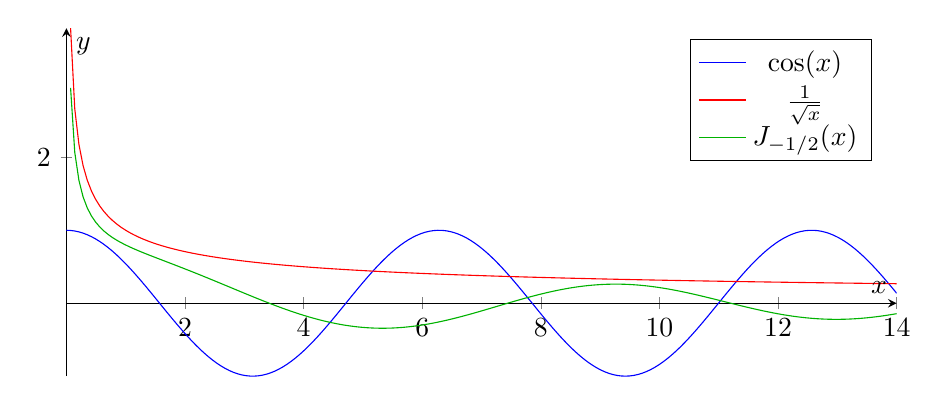
\begin{tikzpicture}
\begin{axis}[
    xlabel=$x$,
    ylabel=$y$,
    domain=0:14,
    samples=200,
    legend pos=north east,
    axis lines=middle,
    width=1\linewidth,
    height=6cm,
]

% Cosine function
\addplot [blue] {cos(deg(x))};
\addlegendentry{$\cos(x)$};

% 1/sqrt(x) function
\addplot [red] {1/sqrt(x)};
\addlegendentry{$\frac{1}{\sqrt{x}}$};

% Bessel function
\addplot [green!70!black] {sqrt(2/(pi*x))*cos(deg(x-sqrt(x)))};
\addlegendentry{$J_{-1/2}(x)$};

\end{axis}
\end{tikzpicture}
\caption{Plot of $\cos(x)$, $\frac{1}{\sqrt{x}}$, and $J_{-1/2}(x)$}
\label{fig:fig-1}
\end{figure}

It shows the Bessel function,$J_{-\frac{1}{2}}$ , is the product of $\frac{1}{\sqrt{x}}$ and $\cos(x)$ which are plotted differently. It is seen that at $x=0$, $\frac{1}{\sqrt{x}}$ goes to infinity and as x increases the $\frac{1}{\sqrt{x}}$ term decreases rapidly as shown. The product of the two functions $(\cos(x)$ and $\frac{1}{\sqrt{x}}$) gives the resulting plot of $J_{-\frac{1}{2}}(x)$. It is seen that the zero points are maintained so $J_{-\frac{1}{2}}(x)$ has the periodicity of $\cos(x)$ but the lobes or amplitude of $J_{-\frac{1}{2}}(x)$ goes on decreasing in value as x increases. Let us see some more plots of the Bessel functions, $J_n(x)$ for different values of n. Figure~\ref{fig:bessel-functions} shows the plot of Bessel functions of positive order $J_{n}(x)$.
\begin{figure}[h]
\centering
\includegraphics[width=1\linewidth]{/graphics/BesselJ_800}
\caption{Plot of Bessel functions of positive order $J_{n}(x)$}
\label{fig:bessel-functions}
\end{figure}

We will proceed to consider the \emph{Bessel function of the second kind} also called the \emph{Neumann function}\index{neumann function} as a second solution to the Bessel equation when n is an integer. It is given by: 
\begin{align}
Y_n = \frac{\cos(n\pi) J_n(x) - J_{-n}(x)}{\sin(n\pi)}
\label{eqn:neumannfunctions}
\end{align}
As we have seen from the plot of $J_n(x)$ that every Bessel function of the first kind has a zero value at the centre i.e at $x= 0$ except for $J_-{\frac{1}{2}}(x)$ and $J_0(x)$, where $J_0(x)$ has a peak value at $ x= 0$. Suppose we want to confine the wave such that it is within a single lobe of the function then the solution is of the order of $n =0$ which is $J_0(x)$. On the other hand, the Neumann functions always start from $-\infty$ at $x=0$ (centre of the waveguide) as shown in Figure~\ref{fig:fig-3}.
\begin{figure}[h]
\centering
\includegraphics[width=1\linewidth]{/graphics/BesselY_800}
\caption{ Plot of the Neumann functions}
\label{fig:fig-3}
\end{figure}

In general, we will have a solution of the form if n is an integer
\begin{equation*}
y(x) = AJ_n(x) + B Y_n(x)\quad\text{where A and B are constants.}
\end{equation*}
In reality, since $Y_n(0) = -\infty$, it makes no physical sense in electromagnetics and electrodynamics so the solution will be 
\begin{equation}
y(x) = AJ_n(x)
\end{equation}
This concludes the discussion on Bessel functions and next, we will discuss circular waveguides. So in this chapter, we looked at a general introduction to Bessel functions and as electrical engineers, these functions play a very important role in cylindrical symmetry. For the circular waveguide which we will discuss in the next chapter, the Bessel function of the first kind is important in its analysis. Another area of waveguide that concerns itself with Bessel functions is dielectric waveguides such as the optical fibre. In their analysis, we consider the function called the \emph{Hankel function}\footnote{
Hermann Hankel(14/02/1839\textemdash29/08/1873), was a German mathematician, known for his contributions to mathematics, specifically in the field of special functions. He developed the Henkel function, also known as the Hermann Henkel function, which is a solution to a certain class of ordinary differential equations. Henkel's work on the Henkel function has found applications in various areas of physics, engineering, and mathematical analysis. His contributions have had a significant impact on the understanding and utilization of special functions in mathematical research and practical applications.
}\index{henkel function} which is the \emph{Bessel function of the third kind}. It is basically an exponentially decaying function equivalent to the $e^{-\alpha x}$ kind of function for the dielectric waveguide.

% \chapter[Circular Waveguide]{CIRCULAR WAVEGUIDE}
	Before we discuss the solution for the circular waveguide let us review what we discussed in the previous lecture and then discuss some important characteristics of the Bessel function when the order n is an integer.\\
	
	So as we have discussed, for a second order PDE of the form 
	 \begin{displaymath}
	 	x^2\frac{d^2y}{dx^2} + x\frac{dy}{dx} + (x^2-n^2)y {=} 0
	 \end{displaymath}
	 It is called a Bessel equation and one kind of the solution is called the Bessel function of the first kind given as an infinite series
	 \begin{displaymath}
	    J_n(x) {=} \sum^\infty_{k=0} \frac{(-1)^k (\frac{x}{2})}{k!\Gamma(n+k+1)}
	 \end{displaymath}
	 where n is the order of the solution and $\Gamma(n+k+1){=}(n+k)\Gamma(n+k)$. As we know for any second order PDE there is always two different independent solution and so we have another solution called the Bessel function of second kind or Neumann function given as 
	 \[Y_n(x) = \frac{\cos(n\pi)J_n(x)-J_{-n}(x)}{\sin(n\pi)} \]
	 In general the solution of the Bessel equation is \[y(x) = A J_n(x) + B Y_n(x)\]
	 However \[Y_n(0)=\pm\infty\] which means at the centre of a cylindrical symmetry the electromagnetic fields or power density are infinite at the centre which makes no physical sense. So due to practical reasons the solution of the Bessel function is 
	 \[y(x) = A J_n(x) \]
	 There is also the Bessel function of the third kind called the Henkel functions and they play important role in electro magnetics when dealing with dielectric waveguides such as the optical fibre where inside the waveguide we have the Bessel function of the first kind and outside the waveguide we have the Bessel functions of the third kind or Henkel functions.\\
	 
	 For all electromagnetic problem the order 'n' is always an integer. So we will have forms such as $ J_0(x) $, $ J_1(x) $, $ J_2(x) $, . and so on. Where only $J_0(x)$ has some value at x{=}0 while the rest value of n is zero is 
	 \[ J_n(0)=0 \; for \; n \neq 0 \]
	 If we plot these functions, we observe that the behaviour in similar to the sine and cosine function (which means it is periodic) but as x increases the peak value starts decreasing. For instance if we plot $J_0(x)$ as shown it peaks at x=0 and attenuates as x increases.
	 
	 \begin{figure}[H]
	 	\centering
	 	\includegraphics[height=5cm]{fig_1.1}
	 	\caption{}
	 	\label{fig:fig1}
	 \end{figure}
	 
	 
	 As we go to higher order functions the behaviour is similar to a sine function. Let's plot the $J_1(x)$ function as shown.
	 
	 \begin{figure}[H]
	 	\centering
	 	\includegraphics[height=5cm]{fig_2.1}
	 	\caption{}
	 	\label{fig:fig2}
	 \end{figure}
	 
	 So when looking for the solution for the waveguide there are two constraints involved and they are;
	 \begin{enumerate}
	 	\item What order n do we have for the solution.
	 	\item Which zero point (root) are we considering because the electric field has to get to zero point (root) at the boundary.
	 \end{enumerate}
	 So the first constraint, n tell us how the wave oscillate while the second constraint which we will denote with p, will tell us which zero point we are considering. 
	 \paragraph{} Therefore, a solution would be specified as $J_n^p(x)$ which gives a specific unique solution. For all possible solutions $J_n^p(x_{np})$, there would be a unique value of $x_{np}$, where $J_n^p(x_{np})=0$ given by the table below.
	 \begin{center}
	 	\begin{tabular}{|c|c c c|}
	 		\hline 
	 		\backslashbox{p}{n} & n=0 & n=1 & n=2 \\ 
	 		\hline 
	 		1&  2.405&  3.832& 5.136 \\ 
	 		
	 		2&  5.520&  7.016& 8.417 \\ 
	 		\hline 
	 	\end{tabular} 
	 \end{center}
	  The table above as we see tells us where the cut-off frequencies occurs for the circular waveguide. n and p in the circular waveguide is similar to m and n in the rectangular waveguide in a way such that they define the modes and the cut-off frequencies for each mode. We recall from the rectangular waveguide that m shows the number of peaks in the x direction while n shows the number of peaks in the y direction. However, in this case the two arguments n and p show what order of the solution and root of the solution we are considering.\\
	 
	 Now let's find the solution of the circular waveguide. Later on we will discuss the derivative of the Bessel function because it is needed in the solution of the waveguide when applying boundary condition.
	 
	 \section{TM mode in Circular Waveguide}
	 So we are considering a hollow metallic pipe of radius a, filled with a dielectric material of $\mu$ and $\epsilon$ as shown.
	 
	\begin{figure}[H]
		\centering
		\includegraphics[width=0.7\linewidth]{fig_3.1}
		\caption{}
		\label{fig:fig3}
	\end{figure}
	 
	 For the Helmholtz wave equation 
	 \begin{equation}
	 	\bigtriangledown^2\vec{E} + w^2\mu\epsilon\vec{E}=0
	 	\label{eqn12.1}
	 \end{equation}\
	 The Laplacian term $\bigtriangledown^2\vec{E}$ has components in the transverse plane and longitudinal. We are still interested in the solution which is of the form of $\vec{E}=\vec{E}_{\bot}e^{-\gamma z}$ where the amplitude $\vec{E}_\bot$ remain in the transverse plane and the wave is propagating in the z direction with propagation constant $\gamma$. \\
	 So we will write equation \ref{eqn12.1} as:
	 \[\bigtriangledown^2\vec{E}_\perp e^{-\gamma z} + \omega^2 \mu\epsilon E_\perp e^{-\gamma z} = 0\]
	 where \[\bigtriangledown^2 = \bigtriangledown^2_\perp + \frac{\partial^2}{\partial z^2}\]
	 So 
	 \[\bigtriangledown^2_\perp\vec{E}_\perp e^{-\gamma z} + \frac{\partial^2}{\partial z^2}\left(\vec{E}_\perp e^{-\gamma z}\right) + \omega^2\mu\epsilon\vec{E}_\perp e^{-\gamma z} = 0\]
	 \[\bigtriangledown^2_\perp\vec{E}_\perp e^{-\gamma z} + (\gamma^2)\left(\vec{E}_\perp e^{-\gamma z}\right) + \omega^2\mu\epsilon\vec{E}_\perp e^{-\gamma z} = 0\]
	 \[\bigtriangledown^2_\perp\vec{E}_\perp e^{-\gamma z} + (\omega^2\mu\epsilon + \gamma^2)\left(\vec{E}_\perp e^{-\gamma z}\right) = 0\]
	 \begin{equation}
	 	\bigtriangledown^2_\perp\vec{E}_\perp + (\omega^2\mu\epsilon + \gamma^2)\vec{E}_\perp = 0
	 	\label{eqn12.2}
	 \end{equation}
	 where $h^2 = \omega^2\mu\epsilon + \gamma^2$. To solve this equation we will use the cylindrical coordinate system. We recall for the rectangular waveguide, we used the Cartesian coordinate system because irrespective of the location we consider along x in the transverse plane the limits along y direction is the same. However for a circular waveguide whose transverse plane is a circle, the limits of y at any location along x changes and so it is preferable to solve the equation using the cylindrical coordinate system because the wave guide has a cylindrical symmetry.\\
	 
	 The cylindrical coordinate system is defined by $\hat{r}$ and $\hat{\phi}$ in the transverse plane and $\hat{z}$ in the longitudinal direction.
	   
	 \begin{figure}[H]
	   	\centering
	   	\includegraphics[height=5cm]{fig_4.1}
	   	\caption{}
	   	\label{fig:fig4}
	 \end{figure}
	   
	   
	 We will now write equation \ref{eqn12.2} for the cylindrical coordinate as 
	   
	 $$
	 \frac{1}{r}\frac{\partial}{\partial r}(r\frac{\partial^2\vec{E}_\bot}{\partial r}) + \frac{1}{r^2}\frac{\partial^2\vec{E}_\bot}{\partial\phi^2}+ h^2\vec{E}_\bot = 0 
	 $$
	 which is the equation which will give the solution of the modes. 
	 \\ The field components in the circular waveguide are $E_r$, $E_\phi$ and $E_z$ as shown
  
     \begin{figure}[H]
       	\centering
      	\includegraphics[height=5cm]{fig_5.1}
       	\caption{}
       	\label{fig:fig5}
     \end{figure}
   
	  For the TM mode we know that $H_z=0$ and $E_z$ exists and for the TE mode $E_z=0$ and $H_z$ will exist. Therefore, for the TM mode we should solve for $E_z$ with appropriate boundary conditions and for TE mode, we should solve for $H_z$ with appropriate boundary conditions. \\
	  
	  So for the TM mode we will solve for $E_z$ which should vary in r and $\phi$ and propagates in the z direction as shown $E_z(r,\phi, z)=E_z(r,\phi)e^{-\gamma z}$, where $e^{-\gamma z}$ signifies the field is propagating in the z direction. So from the wave equation for the cylindrical coordinate which we have written, we have;
	  \begin{equation}
	  	\frac{1}{r}\frac{\partial}{\partial r}(r\frac{\partial E_z}{\partial r}) + \frac{1}{r^2}\frac{\partial^2 E_z}{\partial\phi^2} + h^2 E_z = 0 
	  	\label{eqn12.3}
	  \end{equation}
	 
	  And we know r and $\phi$ are orthogonal so whatever variation we have in r is not related to the variations in $\phi$ so we can write $E_z(r, \phi)$ as
	  $$
	  E_z(r, \phi) = R(r)\Phi(\phi) 
	  $$
	  using separation of variables where $R(r)$ is a function of r only and $\Phi(\phi)$ is a function of $\phi$ only.
	  \\
	  So we will write equation \ref{eqn12.3} as 
	  $$ 
	  \frac{1}{r}\frac{\partial}{\partial r}(r\frac{\partial(R(r)\Phi(\phi))}{\partial r}) + \frac{1}{r^2}\frac{\partial^2 (R(r)\Phi(\phi)}{\partial \phi^2}) + h^2E_z(r,\phi) = 0
	  $$
	  $$
	  \frac{\Phi(\phi)}{r}\frac{d}{dr}\left(r\frac{dR(r)}{dr}\right) + \frac{R}{r^2}\frac{d^2\Phi(\phi)}{d\phi^2} + h^2 E_z = 0
	  $$
	  Divide through by $E_z(r, \phi)=R(r)\Phi(\phi)$ gives 
	  $$
	  \frac{1}{rR(r)}\frac{d}{dr}\left(r\frac{dR(r)}{dr}\right) + \frac{1}{r^2\Phi(\phi)}\frac{d^2\Phi(\phi)}{d\phi^2} + h^2 = 0
	  $$
	  multiply through by $r^2$
	  $$
	  \frac{r}{R(r)}\frac{d}{dr}\left(r\frac{dR(r)}{dr}\right) + \frac{1}{\Phi(\phi)}\frac{d^2\Phi(\phi)}{d\phi^2} + r^2h^2=0
	  $$
	 \begin{equation}
	     \underbrace{\frac{r}{R(r)}\frac{d}{dr}\left(r\frac{dR(r)}{dr}\right)	+ r^2 h}_{function \; of\; r \; only} 
	   	   + \underbrace{\frac{1}{\Phi(\phi)}\frac{d^2\Phi(\phi)}{d\phi^2}}_{function \; of \; \phi \; only} = 0 
	   	   \label{eqn12.4} 
	 \end{equation}
	    
	  which is true for any value of r and $\phi$. The above equation can only be true if each function is a constant and lets denote the constant as $-n^2$ for the function of $\phi$ only ie. 
	  \begin{equation}
	    \frac{1}{\Phi(\phi)}\frac{d^2\Phi(\phi)}{d\phi^2}=-n^2 \; \; => \;\; \frac{d^2\Phi(\phi)}{d\phi^2} + n^2\Phi(\phi) = 0
	    \label{eqn12.5}
	  \end{equation}
	  And so $\frac{r}{R(r)}\frac{d}{dr}(r\frac{dR(r)}{dr}) + r^2h$ has to be $+n^2$ so that equation \ref{eqn12.4} holds, hence;
	  $$
	  \underbrace{\frac{r}{R(r)}\frac{d}{dr}\left(r\frac{dR(r)}{dr}\right)} + r^2h-n^2=0
	  $$
	  $$
	  \frac{r^2}{R(r)}\frac{d^2R(r)}{dr^2} + \frac{r}{R(r)}\frac{dR(r)}{dr} - r^2h-n^2=0
	  $$
	  Multiply through by $\frac{R(r)}{r^2}$
	  \begin{equation}
	   	\frac{d^2R(r)}{dr^2}+\frac{1}{r}\frac{dR(r)}{dr} + (h^2-\frac{n^2}{r^2})R(r)=0
	   	\label{eqn12.6}
	  \end{equation}
	   
	  which in a Bessel equation and can be compared to 
	  $$
	  \frac{d^2y}{dx^2}+\frac{1}{x}\frac{dy}{dx}+\left(1-\frac{n^2}{x^2}\right)y = 0
	  $$
	  and recall $n^2$ is the constant we introduced. First lets solve the second order ordinary differential equation given in equation \ref{eqn12.5} as
	  $$
	  \frac{d^2\Phi(\phi)}{d\phi^2} + n^2\Phi(\phi) = 0
	  $$
	  whose solution is $\Phi(\phi)\equiv $ either $\sin(n\phi)$ or $\cos(n\phi)$. Whether we choose $\sin(n\phi)$ or $\cos(n\phi)$ is immaterial. It only changes the location of reference $\phi=0$ angle in the $\phi$ direction.\\ 
	  
	  By convention we choose $\cos(n\phi)$ so that one solution becomes
	  $$
	  \Phi(\phi)=A\cos(n\phi)
	  $$
	  which will be periodic about $2\pi$ if n is an integer so n has to be an integer.\\
	  
	  Also the solution of the Bessel equation, equation \ref{eqn12.6} is a Bessel function and it is given as
	  $$
	  R(r)=CJ_n(hr)
	  $$
	  The argument of the Bessel function is hr if we compare the two equation below
	  $$
	  r^2\frac{d^2R(r)}{dr^2} + r\frac{dR(r)}{dr} + ((hr)^2 - n^2)R(r) = 0
	  $$
	  $$
	  x^2\frac{d^2y}{dx^2} + x\frac{dy}{dx} + (x^2-n^2)y=0
	  $$
	  Therefore $E_z(r,\phi) = C_nJ_n(hr)\cos(n\phi)$ where $C_n$ depends on the mode we are considering.\\
	  
	  The other components can be gotten from the expressions below for the transverse field component we have discussed in previous lectures.
	  $$
	  \vec{E}_\bot=\frac{-j\omega\mu}{h^2}\bigtriangledown_\bot\times H_z\hat{z} - \frac{\gamma}{d^2}\bigtriangledown_\bot E_z
	  $$
	  and
	  $$
	  \vec{H}_\bot = \frac{-j\omega\mu}{h^2}\bigtriangledown_\bot\times E_z\hat{z}-\frac{\gamma}{h^2}\bigtriangledown_\bot H_z
	  $$
	  We recall for the TM mode $H_z=0$
	  so
	  $$
	  \vec{E}_\bot=-\frac{\gamma}{h^2}\bigtriangledown_\bot E_z$$ for a lossless medium $$\gamma=j\beta
	  $$
	  therefore 
	  $$
	  \vec{E}_\bot = \frac{-j\beta}{h^2}\bigtriangledown_\bot E_z
	  $$
	  $$
	  \vec{E}_\bot = \frac{-j\beta}{h^2}\left\{\frac{\hat{r}\partial E_z}{\partial r} + \frac{\hat{\phi}}{r}\frac{\partial E_z}{\partial\phi} \right\}
	  $$
	  so that 
	  $$
	  E_r=\frac{-j\beta}{h^2}\frac{\partial}{\partial r}E_z = \frac{-j\beta}{h^2}C_nJ'_n(hr)\cos(n\phi)
	  $$
	  $$
	  E_\phi = \frac{-j\beta\partial}{h^2r\partial}E_z = \frac{j\beta n}{h^2 r}C_nJ_n(hr)\sin(n\phi)
	  $$
	  Also for transverse components $H_r$ and $H_\phi$ \\ we have
	  $$
	  \vec{H}_\bot=\frac{j\omega\epsilon}{h^2}\bigtriangledown_\bot\times(E_z\hat{z})
	  $$
	  $$
	  =\frac{j\omega\epsilon}{h^2}\left\{
	  \frac{1}{r}
	  	\begin{tabular}{| c c c |}
	     	$\hat{r}$ &$r\hat{\phi}$ &$\hat{z}$ \\ $\frac{\partial}{\partial r}$ &$\frac{\partial}{\partial\phi}$&0 
	     	\\ 0 & 0 &$\hat{E}_z$
	     \end{tabular}
	     \right\}
	  $$
	  $$
	  H_r=\frac{j\omega\epsilon }{h^2r}\frac{\partial E_z}{\partial \phi} = \frac{-j\omega\epsilon n}{h^2r}C_nJ_n(hr)\sin(n\phi)
	  $$
	  and \[H_\phi = -\frac{j\omega\epsilon}{h^2}\frac{\partial}{\partial r}E_z = -\frac{j\omega\epsilon}{h^2}C_nJ'_n(hr)\cos(n\phi)\]
	  where $J_n'(hr)$ is the derivative of the Bessel function. Now let's determine h by applying the boundary conditions.\\
	  
	  The $E_z$ component is given as $C_nJ_n(hr)\cos(n\phi)$ is parallel or tangential to the conducting wall and so $E_z(r=a)=0$. This implies that $J_n(ha)=0$ which could be any root of a specific Bessel function as n {=} 0,1,2,.... Let's consider n = 0 which is the first order Bessel function $J_0(hr)$. Also n=0 implies that there is a constant field in the $\phi$ direction since $\cos(n\phi)=1$. In general, n shows the number of wavelength, $\lambda$ that fits within $2\pi$ and the order of the Bessel function. For n=0 if we consider the first root of the Bessel function $J_0(hr)$ to satisfy the boundary condition at r=a we have that $h_a = 2.405$ from the table below
	     \begin{center}
	     	\begin{tabular}{| c | c c c |}
	     		\hline
	     		\backslashbox{p}{n} &n{=}0 &n{=}1 &n{=}2 \\
	     		\hline
	     		1 &2.405 &3.832 &5.136 \\
	     		2 &5.520 &7.016 &8.417 \\
	     		\hline
	     	\end{tabular}
	     \end{center}
	     
 
      Also $J_0(ha)=0$ if $ha=5.520$ for the second root at p=2. The first case is called $TM_{01}$ mode and the second case is called the $TM_{02}$ mode.
      
      \begin{figure}[H]
      	\centering
      	\includegraphics[height=5cm]{fig_6.1}
      	\caption{}
      	\label{fig:fig6}
      \end{figure}
      
      Therefore $J_n^p(hr)$ corresponds to $TM_{np}$ mode where n tells us the number of wavelengths $\lambda$ that is in the $\phi$ direction and p tells us the number of lobes that is in the r direction.
      \\ The fundamental TM mode in the $TM_{01}$ mode which has 
      $$
         ha = 2.405 \ \ => \ \ h=\frac{2.405}{a}
      $$
      from $h^2=\gamma^2+w^2\mu\epsilon $ at cut-off, the propagation constant for a lossless medium is zero since $\gamma=j\beta$ and $\beta=0$ as there is no propagation through the conducting wall. 
      \\ So
      $$
        h^2=\omega_c^2\mu\epsilon
      $$ where $\omega_c$ is the cut-off frequency in radians given as $2\pi f_c$ and $f_c$ is the cut-off frequency in Hertz.
      \\So $f_c =\frac{h}{2\pi\sqrt{\mu\epsilon}}$, for $TM_{01}$ mode $h=\frac{2.405}{a}$ therefore 
      $$
      f_c=\frac{2.405}{2\pi a\sqrt{\mu\epsilon}} =\frac{0.383}{a\sqrt{\mu\epsilon}}
      $$
      The second TM mode is the $TM_{11}$ mode where $ha =3.832$ such that $h=\frac{3.832}{a}$ and $f_c=\frac{3.832}{2\pi a\sqrt{\mu\epsilon}}$. Also, the next mode is the $TM_{21}$ mode for which $ha =5.136$ and $h=\frac{5.136}{a} \Longrightarrow f_c=\frac{5.136}{2\pi a \sqrt{\mu\epsilon}}$ and so on. \\
      Let's examine the fundamental mode $TM_{01}$ briefly. Here n=0 which implies that only the fields $E_r, \; E_z \; and \; H_\phi$ exists and they are not varying in the $\phi$ direction. They are given as
      $$
        E_r=\frac{-j\beta}{h^2}C_0J_0'(hr)
      $$
      $$
        E_z=C_oJ_o(hr)
      $$
      and
      $$
        H_\phi=\frac{j\omega\epsilon}{h^2}C_0J_0'(hr)
      $$
      
      From our study of Bessel function of the first order, $J_0(hr)$ is maximum at hr=0 which is the centre of the waveguide so we expect $E_z$ to vary in the r direction such that it is maximum at the centre ant it reduces to zero for the first root at the surface. The two dimensional plots will be treated in the next lecture for different TM modes where we can visually see the changes in the magnitudes of fields in the waveguide.
% \chapter{Circular Waveguide (2)}\label{lec:lec45}
Before delving into the discussion of TE (Transverse Electric) modes in a circular waveguide, let us briefly revisit the TM (Transverse Magnetic) modes covered in the previous chapter. 

\section{TM modes in a circular waveguide}
Considering a circular waveguide filled with a dielectric material characterized by permeability $\mu$ and permittivity $\epsilon$, we recognize the presence of the $E_z$ component. The boundary condition for the conducting surface is fulfilled when $E_z(r=a) = 0$, indicating that the electric field component $E_z$ vanishes at the radial distance $r=a$. Upon solving for $E_z$ using Equation~\eqref{eqn:electricfieldsoln}, we obtained the solution $E_z = A_n J_n(hr)\cos(n\phi)$, where $h = \omega^2\mu + \gamma^2$.

Upon further analysis, we have observed that certain modes satisfy the boundary condition, and these modes can be characterized by two parameters, namely $n$ and $p$. In this context, a specific TM mode is denoted as TM$_{np}$. The parameter $n$ not only represents the variation of the amplitude in $\phi$ but also corresponds to the order of the Bessel function involved in the solution. On the other hand, the parameter $p$ indicates the specific zero point (root) within the Bessel function, which enables the satisfaction of the boundary condition. Indeed, the modes in the circular waveguide are characterized by two aspects. Firstly, the variation of amplitude in the $\phi$ direction. It is represented by the term $\cos(n\phi)$ in the solution.

Secondly, the parameter $n$ determines the number of lobes or wavelengths in the azimuthal direction. Again, the parameter $n$ must be an integer. This is because the term $\cos(n\phi)$ must return to the same value after a complete cycle of $\phi=2\pi$. If the amplitude does not repeat itself after a full revolution, we do not have a mode. So the two values which define a mode are $n$ and $p$ where $n$ is the number of times we have variations in the azimuthal $\phi$, direction and based on the order of the Bessel function $p$, we determine which zero point (root) should be considered to satisfy the boundary condition which in the number of lobes we would get in the radial, $r$, direction.

From our study of the Bessel functions we recall that only $J_0(hr)$ has an amplitude at $hr = 0$ and the rest $J_n(hr)$ function has an amplitude which is zero at $hr = 0$ for $n \ne 0$. Also, we observed from the table that the lowest TM mode is the TM$_{01}$ mode where $n = 0$ and $p = 1$. $n = 0$ implies there is no variation in the $\phi$ direction and $p = 1$ shows that there is only one peak or lobe in the $r$ direction, therefore, $ha = 2.405$ from Table~\ref{tab:rootsofbessel}. 

Now let us look at a colour 2D plot showing the electric field intensities for various TM modes.
\begin{figure}[h]
\centering
\includegraphics[width=0.9\linewidth]{/graphics/colourplot}
\caption{2D colour plot of the TM modes.}
\label{fig:colourplot}
\end{figure}

\subsection{TM$_{10}$ mode}
In the $\phi$ direction, we observe that there is no variation since $n=0$. Also if we consider the $r$ direction, there is one lobe as shown in Figure~\ref{fig:m1}.
\begin{figure}[h]
\centering
\includegraphics[width=0.5\linewidth]{/graphics/m1}
\caption{Plot of Electric field variation in the $r$ direction for TM$_{10}$ mode.}
\label{fig:m1}
\end{figure}

We can observe from the plot that the field peaks at the centre and at zero at the boundary which is the same as the colour plot in Figure~\ref{fig:colourplot}.
   
\subsection{TM$_{02}$ mode}
For the TM$_{02}$ mode, we observe that there is no variation in the azimuthal direction ($\phi$) since $n=0$. This implies that the field intensity remains constant along any circular path drawn in the waveguide.

In terms of the radial direction ($r$), we observe two peaks or lobes. However, it is important to note that these peaks have different magnitudes, which are represented by the red and cyan colours in the plot shown in Figure~\ref{fig:colourplot}. 

To visualize the electric field variation for the TM$_{02}$ mode specifically in the radial direction, let us plot the graph accordingly.
\begin{figure}[h]
\centering
\includegraphics[width=0.7\linewidth]{/graphics/m2}
\caption{Plot of the electric field variation in the $r$ direction for TM$_{02}$ mode.}
\label{fig:m2}
\end{figure}

The plot shown in Figure~\ref{fig:m2} is consistent with the colour plot displayed in Figure~\ref{fig:colourplot}. The magnitude at the centre of the circular waveguide corresponds to the red colour observed in the plot, while the cyan colour represents the negative lobes with lower amplitudes. This observation is in contrast to the behaviour observed in rectangular waveguides, where the amplitude of the electric field remains the same for all lobes.

To illustrate this difference further, let us consider the 3rd order mode in the y direction. The corresponding plot, as shown in Figure~\ref{fig:m3}, demonstrates that the amplitude remains constant throughout the lobes. This is distinct from the behaviour observed in the circular waveguide, where the amplitude varies between the positive and negative lobes.

These distinctions highlight the unique characteristics of the electric field behaviour in different waveguide geometries.
\begin{figure}[h]
\centering
\includegraphics[width=0.5\linewidth]{/graphics/m3}
\caption{Plot of the electric field variation in the $y$ direction for TM$_{x3}$ mode.}
\label{fig:m3}
\end{figure}

\subsection{TM$_{11}$ mode}
As depicted in Figure~\ref{fig:colourplot}, we observe a single wavelength variation in the azimuthal direction ($\phi$). This is evident from the presence of two peaks, one representing the positive maximum and the other representing the negative minimum. The behaviour of these peaks aligns with the first-order Bessel function, specifically $J_1(hr)$.

In the case of this mode, $p=1$, indicating that the boundary condition is satisfied at the first root of $J_1(hr)$. It is important to recall that $J_1(hr)$ has a zero at $h_r=0$, which corresponds to the centre of the circular waveguide. Therefore, the deep blue colour observed in the plot signifies that there is no electric field at the centre of the waveguide.

\subsection{TM$_{21}$ mode}
The TM$_{21}$ mode is characterized by $n=2$, indicating that we expect two wavelengths in the azimuthal direction ($\phi$). This corresponds to the presence of four peaks: two maximums and two minimums, as depicted in Figure~\ref{fig:colourplot}.

Considering $p=1$ for this mode, we anticipate a single peak in the radial direction ($r$). The plot shown in Figure~\ref{fig:m4} illustrates the variation of the electric field in the $r$ direction for the TM$_{21}$ mode.
\begin{figure}[h]
\centering
\includegraphics[width=0.5\linewidth]{/graphics/m4}
\caption{Plot of the electric field variations for TM$_{21}$ mode.}
\label{fig:m4}
\end{figure}

\subsection{TM$_{31}$ mode}
The TM$_{31}$ mode corresponds to $n=3$, indicating three wavelengths in the azimuthal direction ($\phi$). As a result, we observe six peaks or lobes in this direction. Each peak represents a maximum or minimum point of the electric field.

Additionally, considering $p=1$ for this mode means that we apply the boundary condition at the first zero point of the Bessel function. This choice ensures that the electric field satisfies the boundary condition at a specific radial position in the waveguide.

\subsection{TM$_{12}$ mode}
In the case of the TM$_{12}$ mode, we have $n=1$, which corresponds to one wavelength in the azimuthal direction ($\phi$). This results in two lobes or peaks in the $\phi$ direction.

For $p=2$, we consider the second root of the $J_1(hr)$ function. This implies that we expect two lobes in the radial direction ($r$). The colour plot in Figure~\ref{fig:colourplot} for the TM$_{12}$ mode showcases this behaviour, with two distinct lobes in the radial direction.

In summary, the parameter $n$ represents the number of wavelengths in the azimuthal direction ($\phi$), while $p$ denotes the number of lobes in the radial direction ($r$).
   
\section{TE modes in a circular waveguide}
Now, let's take a look at the TE modes of the circular waveguide. For this mode, we need to study the derivative of the Bessel function. From Equation~\eqref{eqn:besselsolnseries2}, we can see that the Bessel function is given as 
\begin{align*}
J_n(x) &= \sum_{k = 0}^{\infty}\frac{(-1)^k (\frac{x}{2})^{2k + n}}{k! \Gamma(n + k + 1)}\quad\text{But, }\Gamma(n + k + 1) = (n+k)!\\
&= \sum_{k = 0}^{\infty}\frac{(-1)^k (\frac{x}{2})^{2k + n}}{k! (n + k)!}\quad\text{Substituting }x = hr\\
J_n(hr) &= \sum_{k = 0}^{\infty}\dfrac{(-1)^k(hr)^{2k + n}}{k!(k+n)!2^{2k + n}} \quad \text{where n is an interger}
\end{align*}
So the derivative of the Bessel function is given as $ \derivative{J_n(hr)}{r} $ and it is denoted by $J'_n(hr) $ and it is given as 
\begin{align*}
J'_n(hr) &= \sum_{k = 0}^{\infty}\dfrac{(-1)^k h^{2k + n}(2k + n)r^{2k + n -1}}{k!(k+n)!2^{2k + n}}\\
&= \frac{1}{2}\bigg[J_{n-1}(hr) - J_{n + 1}(hr)\bigg]\footnotemark
\end{align*}
\footnotetext{
By differentiating $J_n(hr)$ with respect to $r$ and further simplifying the expression, we obtain the above relationship.
}
Indeed, for the circular waveguide, the application of the boundary condition leads us to consider specific numerical values of $hr$ at which the derivative of the Bessel function, $J'_n(hr)$, equals zero. These values of $hr$ are essential for determining the characteristics and properties of the waveguide modes.

However, it is important to note that this relationship and the zeros of the derivative of the Bessel function are particularly useful when dealing with dielectric waveguides, such as optical fibres. In the context of the circular waveguide, we primarily focus on the numerical values that satisfy the boundary condition rather than explicitly utilizing the relationship mentioned.

For further reference and analysis, Table~\ref{tab:zerosofdiffbessel} provides the specific values of $hr$ where $J'_n(hr)$ vanishes, which are crucial for solving the modes of the circular waveguide.
\begin{table}[h]
\centering
\text{Zeros of $J'_n(hr)$}\\
\begin{tabular}{|c | c c c|}
\hline
\backslashbox{p}{n} & n=0 & n=1 & n=2 \\
\hline
1 & 3.832 & 1.841 & 3.054 \\
2 & 7.016 & 5.331 &6.706 \\
\hline
\end{tabular}
\label{tab:zerosofdiffbessel}
\end{table}

From the table, we observe that the lowest zero point is when $n = 1$ and $p = 1$ and this corresponds to a TE$_{11}$ mode therefore the TE$_{11}$ mode is the lowest cut-off mode, followed by TE$_{21}$ and then TE$_{01}$ and so on.

For the TE mode we know that $E_z = 0$ and $H_z$ exists, so we will solve for the $H_z$  component which is given as;
\begin{align*}
H_z(r,\phi,z) = H_z(r,\phi)e^{-\gamma z}
\end{align*}
So, the Helmholtz equation becomes
\begin{equation}
\nabla^2 H_z(r,\phi) + h^2 H_z(r,\phi) = 0
\label{eqn:helmholtztemode}
\end{equation}
To solve this equation we repeat the procedure we carried out for the TM mode such that 
\begin{align*}
H_z(r,\phi)= R(r)\Phi(\phi)
\end{align*}
Therefore Equation~\eqref{eqn:helmholtztemode} becomes
\begin{align*}
\frac{1}{r}\partialderivative{}{r}\bigg(r\partialderivative{R\Phi}{r}\bigg) + \frac{1}{r^2}\partialderivative[2]{R\Phi}{\phi} + h^2\{R\Phi\} = 0
\end{align*}
Thus, the two solutions are given as
\begin{equation}
\derivative[2]{R}{r} + \frac{1}{r^2}\derivative{R}{r} + \bigg(h^2 - \frac{n^2}{r^2}\bigg)R = 0
\label{eqn:radialtemode}
\end{equation}
and 
\begin{equation}
\dfrac{d^2\Phi}{d\phi^2} + n^2\Phi = 0
\label{eqn:angulartemode}
\end{equation}
The procedure is similar to that of the TM mode, the only difference is that we start with solving the Helmholtz wave equation for the magnetic field. So the solution of the magnetic field is 
\begin{align*}
H_z(r,\phi) = A_nJ_n(hr)\cos(n\phi)\quad\text{n has to be an integer}
\end{align*}
We can now solve for the other components. From Equations~\eqref{eqn:transverseele2} and~\eqref{eqn:transversemag2} we have
\begin{align*}
\bar{E}_\perp = \frac{-j\omega\mu}{h^2}\nabla_\perp\times(H_z\hat{z}) - \frac{\gamma}{h^2}\nabla_\perp E_z\\
\bar{H}_\perp = \frac{j\omega\epsilon}{h^2}\nabla_\perp\times(E_z\hat{z}) - \frac{\gamma}{h^2}\nabla_\perp H_z
\end{align*}

For the TE mode, $E_z = 0$, therefore,
\begin{dmath} 
\bar{H}_\perp = H_r \hat{r} + H_\phi \hat{\phi} = \frac{-\gamma}{h^2}\nabla_\perp H_z
= \frac{-\gamma}{h^2}\bigg\{ 
\hat{r}\partialderivative{H_z}{r} + \frac{\hat{\phi}}{r}\partialderivative{H_z}{\phi}  
\bigg\}
\end{dmath}
Therefore
\begin{align*}
H_r = \frac{-\gamma}{h^2}\partialderivative{H_z}{r} = \frac{-\gamma}{h^2}A_nJ'_n(hr)\cos(n\phi)
\end{align*}
For a lossless medium $ \gamma =j\beta$, so 
\begin{align*}
H_r = \frac{-j\beta}{h^2}A_nJ'_n(hr)\cos(n\phi)
\end{align*}
Similarly, for the $\phi$ component, we have
\begin{align*}
H_\phi = \frac{-j\beta}{h^2}\frac{\partial H_z}{\partial \phi} = \frac{-j\beta n}{h^2 r}A_nJ'_n(hr)\sin(n\phi)
\end{align*}

For the transverse electric field, we have
\begin{dmath} 
\bar{E}_\perp = \frac{-j\omega\mu}{h^2}\nabla_\perp\times H_z\hat{z}
=\frac{-j\omega\mu}{h^2}
\left\{ 
\frac{1}{r}
\begin{vmatrix}
\hat{r} & r\hat{\phi} & \hat{z}\\ 
\partialderivative{}{r} & \partialderivative{}{\phi} & 0\\
0 & 0 & H_z
\end{vmatrix}
\right\}
= E_r\hat{r} + E_\phi\hat{\phi}
= \frac{j\omega\mu}{h^2} \bigg\{\frac{1}{r}\partialderivative{H_z}{\phi} - \partialderivative{H_z}{r}\bigg\}
\end{dmath}
Therefore, the components are
\begin{align*}
E_r &= \frac{-j\omega\mu}{h^2 r}\partialderivative{H_z}{\phi} = \frac{j\omega\mu n}{h^2 r}A_nJ_n(hr)\sin(n\phi)\\
E_\phi &= \frac{j\omega\mu}{h^2 }\partialderivative{H_z}{\phi} = \frac{j\omega\mu }{h^2 }A_nJ'_n(hr)\cos(n\phi)
\end{align*}
So the component is
\begin{align}
H_r &= \frac{j\beta}{h^2 }A_nJ_n(hr)\cos(n\phi)\\ H_\phi &= \frac{j\beta}{h^2 r}A_nJ_n(hr)\sin(n\phi)\\
H_z &= A_nJ_n(hr)\cos(n\phi)\\
E_r &= \frac{j\omega\mu n}{h^2 r}A_nJ_n(hr)\sin(n\phi)\\
E_\phi &= \frac{j\omega\mu }{h^2 }A_nJ_n(hr)\cos(n\phi)\\
E_z & = 0
\end{align}

In the context of the circular waveguide, we have observed that the transverse components of the magnetic field, namely $H_r$ and $H_\phi$, are directly related to the derivative of the field component in the longitudinal direction, $H_z$. Specifically, $H_r$ is proportional to $\partialderivative{H_z}{r}$, while $H_\phi$ is proportional to $\partialderivative{H_z}{\phi}$.

Similarly, the transverse components of the electric field, $E_r$ and $E_\phi$, are related to the derivative of the field component in the longitudinal direction, $H_z$. In this case, $E_r$ is proportional to $\partialderivative{H_z}{\phi}$, and $E_\phi$ is proportional to $\partialderivative{H_z}{r}$.

For the TE (Transverse Electric) mode, we specifically observed that the electric field component $E_\phi$ is parallel to the conducting walls of the waveguide. This is illustrated in Figure~\ref{fig:m5}, where the electric field lines are tangential to the walls of the circular waveguide.
\begin{figure}[h]
\centering
\includegraphics[width=0.5\linewidth]{/graphics/m5}
\caption{Azimuthal electric field component for the TE mode}
\label{fig:m5}
\end{figure}

Again, the electric field component $E_\phi$ must go to zero at the boundary ($r=0$) to satisfy the boundary condition. This requirement leads to the condition $J'_n(ha) = 0$, where $ha$ represents the product of the waveguide radius $a$ and the radial component $h$ of the waveguide mode.

By referring to Table~\ref{tab:zerosofdiffbessel}, we can observe that the smallest value of $ha$ for which the boundary condition is satisfied is $ha = 1.841$. This corresponds to the TE mode with the lowest cut-off frequency. In this mode, we have one wavelength variation in the azimuthal direction ($\phi$) due to $n=1$, and $p=1$ indicates that we are considering the first zero point of the derivative of the Bessel function, specifically $J'_1(hr)$.

So
$$
(h)_{\text{TE}_{11}} = \frac{1.841}{a}
$$
And the cut-off frequency of this mode is 
$$
(f_c)_{\text{TE}_{11}} = \frac{(h)_{\text{TE}_{11}}}{2\pi\sqrt{\mu\epsilon}} = \frac{0.293}{a\sqrt{\mu\epsilon}}
$$
We recall that the lowest TE mode is the TE$_{01}$ mode which corresponds to $(f_c)_{\text{TE}_{01}} = \frac{0.383}{a\sqrt{\mu\epsilon}}$. It is worth noting that the cut-off frequency of the TE$_{11}$ mode is lower than that of the TE$_{01}$ mode.

As a result, the TE$_{11}$ mode becomes the dominant mode in the circular waveguide. The modes in the circular waveguide are not arranged in a simple order like in the rectangular waveguide due to the presence of the derivative of the Bessel function in the boundary condition. However, by referring to the table, we can observe that the modes are ordered based on their cut-off frequencies, from lowest to highest, as $\text{TE}_{11}, \text{TE}_{21}, \text{TE}_{01}, \text{TE}_{12}, \text{TE}_{22}$, and $\text{TE}_{02}$.

\section{Attenuation in the circular waveguide}
In terms of losses, the behaviour in the circular waveguide is similar to that of the parallel plane waveguide. The modes that have more energy close to the conducting wall will experience more losses because this energy can excite currents on the conducting surfaces. 

For the TE (Transverse Electric) mode, which includes both the $H_z$ and $H_\phi$ components, and the TM (Transverse Magnetic) mode, which includes the $H_\phi$ component, the losses generally decrease as the frequency increases and then start to increase. This is a common trend. 

However, there are unique modes of the order $\text{TE}_{0p}$. In such modes, the losses decrease monotonically as the frequency increases. This is demonstrated in Figure~\ref{fig:m6} for the specific case of the TE$_{01}$ mode.

It is important to note that the specific loss behaviour in different modes and frequency ranges can vary, but the general trend described above provides an understanding of the behaviour of losses in the circular waveguide.
\begin{figure}[h]
\centering
\includegraphics[width=.5\linewidth]{/graphics/m6}
\caption{Attenuation in the TE$_{01}$ mode}
\label{fig:m6}
\end{figure}

Indeed, the $\text{TE}_{0p}$ mode in the circular waveguide exhibits a unique behaviour where the losses decrease monotonically as the frequency increases. This behaviour is distinct and not observed in any other mode, whether in a circular or rectangular waveguide. Therefore, the $\text{TE}_{0p}$ mode stands out in terms of its loss characteristics. This concludes our discussion on the circular waveguide.


% antenna theory

% 	\chapter{Antenna theory}
\section{Introduction}	

So far we have cruised through understanding electromagnetic waves and not how they were generated. Now it is of concern to us and we ask the question of how the electromagnetic waves are generated. In this chapter we will be answering that question through the topic called radiation. 

Essentially this chapter deals first with the principles of generation of electromagnetic waves and then practical devices which can generate electromagnetic waves from currents and voltages and also convert the electromagnetic waves to currents and voltages- which is called an \textbf{Antenna}.

\section{Radiation}
The basis of radiation is the \textbf{accelerated charges}. From electrostatics, when there is a charge, then there is essentially electric field. If the charge is kept in motion, then it constitute current and current produces magnetic field but this current is in uniform motion. However what happens when there is time varying current (a current which varies as a function of time and therefore it gets accelerated and decelerated), what kind of field would exist? Well, the answer is simple, as stated earlier, accelerated charges is the basis of radiation and radiation is the propagation of electromagnetic field.

However, every accelerated charge may not give you radiation because if it would, a simple coaxial cable having time varying currents should produce radiation but that is not what happens. Well one other condition has to be satisfied. Lets consider a transmission line as shown below for the example we considered earlier - a coaxial cable - where the distance between the lines is far less than the wavelength of the time varying signal flowing through the transmission line.

\begin{figure}
	\centering
	\includegraphics[height=5cm]{fig_1}
	\caption{Transmission line}
\end{figure}

As discussed in previous chapter, the transmission line completely guides the electromagnetic energy within its structure. This can be understood from the current standing wave equation given by
$$I(l)=\dfrac{V^+}{Z_o}e^{-\gamma l} - \dfrac{V^-}{Z_o}e^{-\gamma l}$$
The components of the equation shows that the traveling currents are traveling in opposite direction as shown in fig 1.1. Essentially the field produced by each of the time varying components cancel out because the distance between the lines is extremely small (d$\ll\lambda$). 

So though we have accelerated and decelerated charges, we do not have radiation. However we can say that there is a possibility of radiation because accelerated and decelerated charges are capable of giving radiation.
\begin{figure}
	\centering
	\includegraphics[height=5cm]{fig_1}
	\caption{Transmission line}
\end{figure}
However if the distance between the lines in fig 1.1 are separated further such that $d\approx\lambda$ as shown in fig 1.2, then the cancellation will not take place in all direction. For instance if it cancels in one direction, in some other direction it is possible that phase of the wave is changed due to phase difference between propagating waves of the two currents and there might be radiation from the structure.
Therefore, it appears that radiation has two conditions which are; 
\begin{enumerate}
	\item There must be time varying currents; and
	\item There must be spatial imbalance of the currents.
\end{enumerate}

Now lets identify structures where these conditions are clearly specified.

\subsection*{RADIATION PHENOMENA}
With these points it is important to note that as frequency increases, the acceleration and deceleration of charges will increase because the rate at which the current is changing is higher. Hence as frequency increase for the same amplitude of currents, same peak current or RMS current, we should get more radiation. What we have designed in fig1.2b is essentially an antenna; and in designing any antenna, we will want the structure to give radiation effectively, also we will want the structure to transfer sufficient amount of power in the form of EM waves which will take the power away from the structure.

Just as an illustration we take a transmission line whose characteristic impedance is known and then flare the end of the structure so that $d\approx\lambda$ such that there is possibility of radiation.

Recall that the characteristic impedance of a transmission line (TL) depends on L and C which are the inductance per unit length and capacitance per unit length respectively. For effective power transfer we recall that the impedance of the load end (which in this case is the impedance seen by the wave as it propagates from the guided structure to space) must match the characteristic impedance $Z_o$. So if we strive to maintain maximum power transfer then the end of the TL is controlled (gradual) such that characteristic impedance at the end of the TL just matches the impedance seen by the wave which is 377$\Omega$ for free space.
By controlling the flaring we vary L and C and thus vary $Z_o$
\begin{figure}
	\centering
	\includegraphics[height=5cm]{fig_2}
	\caption{Flared transmission line}
\end{figure}
Also we can take an extreme case and still have the nature of of standing wave retained in the TL when the ends are flared completely as shown in fig 1.3b. In this case the current distribution is in the same direction and is generating field which will not cancel each other.

While we would be discussing the topic, we would give answers to question like how much power is radiated and which direction would the power not be radiated. What kind of polarization will be developed by the structure? and so on.

Considering an antenna structure, we would say the structure has dual nature that is on one side, it acts as a circuit element with input impedance and bandwidth range, while on the other side it generates electric and magnetic fields with characteristics (in what direction does the wave propagate) and the power the fields radiate.
\begin{figure}
	\centering
	\includegraphics[height=5cm]{fig_3}
	\caption{Antenna characteristics}
\end{figure}

\begin{itemize}
	\item \textbf{Circuit characteristics}
	\item Input Impedance
	\item Bandwidth
\end{itemize}

\begin{itemize}
	\item \textbf{Wave Characteristics}
	\item Kind of Polarization
	\item Power Radiated
	\item Directional Characteristics
\end{itemize}
Essentially, when investigating antennas, we consider the dual nature and concern ourselves with the input side when the antenna acts as a circuit element as well as treat it as a source of electromagnetic waves and provide their characteristics. 

\section{Mathematical Modeling of Radiation}
To model the problem of radiation, we refer back to Maxwell's Equation. In previous chapters, when modeling electromagnetic waves we considered both source free medium and a medium with finite conductivity. In a medium of finite conductivity we had conduction current density, but in this case we would separate these two medium when modeling radiation. One region would be the source region where there is current and charges and there is a different region where there would be the electric and magnetic fields.
\begin{figure}
	\centering
	\includegraphics[height=5cm]{fig_4}
	\caption{Mathematical model}
\end{figure}

Lets consider a source of conduction current density $\vec{J}$ and volume charge density $\rho$ which produces electric and magnetic fields at some point called the observation point which source free as shown in Fig 1.5 The objective would be establishing the relationship between the electric and magnetic fields with the sources.

Some point to note in this analysis are;
\begin{itemize}
	\item Previously when analyzing EM wave (the uniform plane wave) the source was pushed to infinity while here, the sources are at an observable distance from the point of reference.
	\item When we analyzed the uniform plane wave we where not concerned with the choice of coordinate system to use and it was possible to model in the cartesian coordinate system which was an easier choice because the coordinates are not changing with direction but in this case the choice of coordinate system matters and the appropriate choice is the spherical coordinate system.
\end{itemize}

So the coordinate system normally used for antennas is the spherical coordinate system, as shown below

\begin{figure}
	\centering
	\includegraphics[height=5cm]{fig_5}
	\caption{Spherical coordinate}
\end{figure}

With that established lets reference the maxwell's equations given below

$$(i) \nabla\cdot\vec{D} =\rho 
\ or\ \nabla \cdot\vec{E} =\dfrac{\rho}{\epsilon} $$	
$$(ii) \nabla\cdot\vec{B}=0$$	
$$(iii)\nabla\times\vec{E}=- \dfrac{\partial\vec{B}}{\partial t}$$
$$(iv)\nabla\times\vec{H}=\bar{J}+\dfrac{\partial\bar{D}}{\partial t}$$

From (ii) $\nabla\cdot\vec{B}=0$ the condition is still satisfied, if it is rewritten as $\nabla\cdot(\nabla\times\vec{A})=0$, and we call the vector $\vec{A}$ the magnetic vector potential. Recall from the electrostatic case that calculating for the electric field for any problem was best approached by finding the scalar potential and this approach is applied here such that $\vec{B}=\nabla\times\vec{A}$ which simplifies the solution.

Our objectives are as follows;\\
1) Find the solution for the potential A\\
2) Find the magnetic and electric fields and \\
3) Find the power radiated from the sources
\\
From (iii) $$\nabla\times\vec{E}=\dfrac{-\partial(\nabla\times\vec{A})}{\partial t}$$

interchanging the time and space derivatives gives
$$\nabla\times\vec{E}=-\nabla\times\dfrac{-\partial\vec{A}}{\partial t}$$

Let represent a time derivative with a dot ($\cdot$) on the vector
$$\nabla\times\vec{E}=-\nabla\times\dot{\vec{A}};$$

$$\nabla\times(\vec{E}+\dot{\vec{A}})=0;$$ Still the expression can be written as;

$$\vec{E}+\dot{\vec{A}}= -\nabla V$$ since $\nabla\times(-\nabla V)=0$

The minus sign is placed to retain the relationship between $\vec{E}$ and $V$. If the time varying magnetic scalar vector $\dot{\vec{A}}$ is removed from the expression

From (iv)
$\nabla\times\vec{H}=\vec{J}+\dot{\vec{D}}$
and $\vec{D}=\epsilon\vec{E}$

Then,

$\nabla\times\vec{H}=\vec{J}+\epsilon\dot{\vec{E}}$ (we assume $\epsilon$ is not a function of time - a homogeneous medium) \\

From $\vec{B}=\nabla\times\vec{A}$, $\vec{B}=\mu\vec{H}$
\begin{equation}
\mu\vec{H}=\nabla\times\vec{A}
\end{equation}
\begin{equation}
\vec{H}=\dfrac{1}{\mu}\nabla\times\vec{A}
\end{equation}


Substitute equation 1.1 in 1.2 gives $$\nabla\times(\dfrac{1}{\mu}\nabla\times\vec{A})=\vec{J}+\epsilon\dot{\vec{E}}$$

Also $\mu$ is not a function of space (isotropic)

$$\nabla\times\nabla\times\vec{A}=\mu\vec{J}+\mu\epsilon\dot{\vec{E}}$$ 

Using vector identities
$$\nabla\times\nabla\times\vec{A}= \nabla(\nabla\cdot\vec{A}) -\nabla^{2}\vec{A}=\mu\vec{J}+\mu\epsilon\dot{\vec{E}}$$

Substituting $\dot{\vec{E}}=-(\nabla\dot{V}+\ddot{\vec{A}})$

$$\nabla(\nabla\cdot\vec{A}) -\nabla^{2}\vec{A}=\mu\vec{J}+\mu\epsilon(-(\nabla\dot{V}+\ddot{\vec{A}}))$$
$$=\mu\vec{J}+\mu\epsilon\nabla\dot{V}-\mu\epsilon\vec{A}$$ 
Rewriting the expression
\begin{equation}
\nabla^{2}\vec{A}-\mu\epsilon\ddot{\vec{A}}=-\mu\vec{J}+\mu\epsilon\nabla\dot{V}+\nabla(\nabla\cdot\vec{A})
\end{equation}


When the above expression is compared with the equation of electric and magnetic fields in a source free unbound medium (set $\vec{J}$ to zero for $\sigma=0$) It is seen that the above expression has the components $\mu\epsilon\nabla\dot{V}+\nabla(\nabla\cdot\vec{A})$ in addition to the equations of electric and magnetic fields in a source free unbounded medium given below
$$\nabla^{2}\vec{E}-\mu\epsilon\ddot{\vec{E}}=0$$
$$\nabla^{2}\vec{H}-\mu\epsilon\ddot{\vec{H}}=0$$


If these solutions satisfy the same boundary condition- it is source free and an unbound medium- then from the uniqueness theorem they are indeed the same solution. Hence we can make equation 1.3 unique by satisfying the uniqueness theorem and defining the expression for the divergence of the vector 'A'.

Hence, \begin{equation}
\mu\epsilon\nabla\dot{V}+\nabla(\nabla\cdot\vec{A})=0 \Rightarrow \nabla(\mu\epsilon\dot{V}+\nabla\cdot\vec{A})=0
\end{equation}

then
$$\nabla\cdot\vec{A}=-\mu\epsilon\dot{V}$$

which is called the Lorentz Gauge condition.
This condition defines the divergence of the magnetic vector potential
Now equation 1.3 reduces to
\begin{equation}
\nabla^{2}\vec{A}-\mu\epsilon\ddot{\vec{A}}=-\mu\vec{J}
\end{equation} 


Take the divergence of $\vec{E}+\dot{\vec{A}}=-\mu\vec{J}$ to give;

$$\nabla\cdot\vec{E}+\nabla\cdot\dot{\vec{A}}=-\nabla^{2} V$$\\
substituting	
$$\nabla\cdotp\dot{\vec{A}}=-\mu\epsilon\ddot{V}$$
$$\nabla\cdotp\vec{E}-\mu\epsilon\ddot{V}=-\nabla^{2} V$$

Rearranging; $\nabla^{2} V-\mu\epsilon\ddot{V}=-\nabla\cdotp\vec{E}$

From $\nabla\cdotp\vec{E}=\dfrac{\rho}{\epsilon}$, We get;
\begin{equation}
\nabla\dot\vec{E}-\mu\epsilon\ddot{V}=-\dfrac{\rho}{\epsilon}
\end{equation}

Both equations 1.5 and 1.6 can be rewritten as
\begin{center}
	$\Box\vec{A}=\mu J$\\
	$\Box V=\dfrac{\rho}{\epsilon}$\\
\end{center}
where $\Box$ is called the D'Alembertian Operator or box operator given by 

$$\Box=\dfrac{\partial^{2}}{\partial t^{2}}-\dfrac{1}{c^{2}}\nabla^{2}$$

With Lorentz gauge condition we get an identical solution to equation 1.6 for the scalar potential V. This expression shows that the magnetic vector potential is related to the conduction current density $\vec{J}$ and the scalar potential is related to the volume charge density $\rho$. In conclusion, when we have time varying sources, we would have electric potential and magnetic vector potential and both are essentially governed by the wave equation; which implies they have wave behaviour in the 3 dimensional space.
% \chapter{Green Function Technique}
Now, we would solve the wave equations in Equations~\eqref{eqn:vectorpotentialeqnwithlorentzguage} and~\eqref{eqn:scalarpotential} using a technique known as the \emph{Green Function Technique}\index{green function technique}. The Green function technique is applied in solving inhomogeneous ordinary differential equations which, in this case, is what we have. The Green function technique solves for the Green function, which is a scalar denoted by $G$ for the differential equations given. The Green function, $G$, is the impulse response of the differential equation. For the wave equation, the green function, $G$, is the spatial impulse response of the system which is described by the wave equations. When applying the Green function technique to the wave equations given, we are essentially solving for the spatial impulse response of the wave equations. The spatial impulse response of the wave equations is the solution to the wave equations. The solution to the wave equations is the fields $\vec{E}$ and $\vec{H}$. The wave equations from in Equations~\eqref{eqn:vectorpotentialeqnwithlorentzguage} and~\eqref{eqn:scalarpotential} are given by:
\begin{align}
\nabla^{2}\bar{A}-\mu\bar{A} = -\mu\bar{J}
\label{eqn:vectorpotentialeqnwithlorentzguage_lec47}\\
\nabla^{2}V-\mu\epsilon\frac{\partial V}{\partial t} = -\frac{\rho}{\epsilon}
\label{eqn:scalarpotential_lec47}
\end{align}
Let us note that the Laplace operator is scalar (it operates on a scalar) which means it operates on each component of the $\bar{A}$ vector. So essentially replacing the vector $\bar{A}$ with a scalar is possible.
Points to note when using the technique:
\begin{enumerate}[(i)]
\item First, we replace in the differential Equations~\eqref{eqn:vectorpotentialeqnwithlorentzguage_lec47} and~\eqref{eqn:scalarpotential_lec47}, the original function (in this case, $\bar{A}$ and $V$) with the Green function and replace the driving quantity (in this case $-\mu\bar{J}$ and $-\frac{\rho}{\epsilon}$) with the impulse function $\delta = f_{n}$(space).
\item Next, we convolve the solution of the Green function with the driving quantity to get the solution to the original function.
\end{enumerate}

\subsection{Green Function for the Vector Potential}
Before applying the Green function technique, we know that the fields $\vec{E}$ and $\vec{H}$ are time-varying fields and so, $\vec{A}$ is also a time-varying field and vary with respect to $e^{j\omega t}$, hence,
\begin{align*}
\partialderivative{}{t} \equiv j\omega\quad\text{and}\quad\partialderivative[2]{}{t} \equiv j\omega.j\omega = -\omega^{2}
\end{align*}
Therefore, factoring in the time quantity would give the following equation for the vector potential:
\begin{align}
\nabla^{2}\bar{A}-\omega^{2}\mu\bar{A} = -\mu\bar{J}
\label{eqn:vectorpotentialeqnwithlorentzguage_lec47_timevarying}
\end{align}
Recall from the wave equation, in an inbound medium,
\begin{align*}
\beta^{2} &= \omega^{2}\mu \varepsilon\\
\beta &= \omega\sqrt{\mu \varepsilon}\\
\beta &= \omega\sqrt{\mu_o \varepsilon_o}\quad\text{for free space}
\end{align*}
So, Equation~\eqref{eqn:vectorpotentialeqnwithlorentzguage_lec47_timevarying} can be written as:
\begin{align*}
\nabla^{2}\bar{A}+\beta^{2}\bar{A} = -\mu\bar{J}
\end{align*}
Applying the Green function technique, then,
\begin{align*}
\nabla^{2}\bar{G}+\beta^{2}\bar{G} = \delta(\text{space})
\end{align*}
Solving the equation in the spherical coordinate system,
\begin{dmath*}
\partialderivative{}{r} \left(r^{2} \partialderivative{G}{r} \right) + \frac{1}{r^2 \sin \theta} \partialderivative{}{\theta}\left(\sin \theta \partialderivative{G}{\theta}\right) + \frac{1}{r^{2}\sin^{2}\theta} \partialderivative[2]{G}{\phi} + \beta^{2}G = \delta(r,\theta,\phi)
\end{dmath*}

Considering the source at the origin (impulse located at origin) simplifies the solution because at whatever direction in space, you see the same source which makes the solution for the equation spherically symmetric. Hence, $G$ is not a function of $\theta$ and $\phi$ and $\derivative{}{\theta} \equiv \derivative{}{\phi} = 0
$. Thus, the differential equation becomes:
\begin{equation}
\derivative{}{r}\left(r^{2}\derivative{G}{r}\right) +  \beta^{2}G = \delta(r)\footnotemark
\label{eqn:vectorpotentialeqnwithlorentzguage_lec47_sphericalcoordinates}
\end{equation}
\footnotetext{
Notice the partial derivatives are converted to full derivatives because $G = f_{n}(r)$ only.
}
Let's define a variable $\psi = rG$, such that,
\begin{align*}
&\derivative{\psi}{r} = r\derivative{G}{r} + G&\\
&\derivative{G}{r} = \frac{1}{r}{\derivative{\psi}{r} - G}&\\
&\text{and}&\\
&G = \frac{\psi}{r}&
\end{align*}
Substitute $G$ and $\derivative{G}{r}$ interms of $\psi$ in Equation~\eqref{eqn:vectorpotentialeqnwithlorentzguage_lec47_sphericalcoordinates}:
\begin{align*}
\frac{1}{r^{2}}\derivative{}{r}\left(r^{2}
\left(\frac{1}{r}(\derivative{\psi}{r} - G) \right) \right) + \beta^{2}\frac{\psi}{r} &= \delta(r)\\
\frac{1}{r^{2}}\derivative{}{r}\left(r\derivative{\psi}{r} - rG \right) + \beta^{2}\frac{\psi}{r} &= \delta(r)\\
\frac{1}{r^{2}}\derivative{}{r}\left(r\derivative{\psi}{r} \right) - \frac{1}{r^{2}}\derivative{}{r}(rG) + \beta^{2}\frac{\psi}{r} &= \delta(r)\\
\frac{1}{r^{2}}\left(r\derivative[2]{\psi}{r} + \derivative{\psi}{r} \right) - \frac{1}{r^{2}}\derivative{\psi}{r} + \beta^{2}\frac{\psi}{r} &= \delta(r)\\
\frac{1}{r}\derivative[2]{\psi}{r} + \frac{1}{r^{2}}\derivative{\psi}{r} - \frac{1}{r^{2}}\derivative{\psi}{r} + \beta^{2}\frac{\psi}{r} &= \delta(r)\\
\frac{1}{r}\left(\derivative[2]{\psi}{r} + \beta^{2}\psi \right) = \delta(r)
\end{align*}
\begin{equation}
\derivative[2]{\psi}{r} + \beta^{2}\psi = \delta(r)\label{eqn:greenfunction}
\end{equation}
Equation~\eqref{eqn:greenfunction} has the solution $\psi = Ce^{-j\beta r} + De^{j\beta r}$. The two terms represent the travelling waves in the direction of $r$ and $r$ is always positive in the spherical coordinate system. The first term represents a wave which is travelling in all positive directions, i.e. away from the origin, while the second term represents a wave that is travelling in the negative $r$ direction but $r$ is always positive, so it represents a wave that is moving towards the origin. Since our source is at the origin and there is no energy source elsewhere in the medium, then this wave does not exist. The solution now reduces to:
\begin{align*}
\psi = Ce^{-j\beta r}
\end{align*}
But recall $G = \frac{\psi}{r}$, hence the solution for the Green function is:
\begin{align}
G = \frac{Ce^{-j\beta r}}{r}
\label{eqn:greenfunction_solution}
\end{align}
\begin{figure}[h]
\centering
\includegraphics[width=\linewidth]{/graphics/img_1}
\caption{Spherical wave}
\label{fig:sphericalwave}
\end{figure}

It should be noted that a constant $r$ represents the constant phase surface. In the spherical coordinate system when $r$ equals a constant, we know it represents a sphere so these constant phase surfaces are spheres and the wave propagating is called the \emph{spherical wave}\index{spherical wave}. Also, one other thing to be noted is that the amplitude of the spherical wave reduces by $\frac{1}{r}$ as opposed to the uniform plane wave in which the amplitude does not change as a function of space. In conclusion, the solution of the Green function, $G$, gives a spherical wave whose magnitude reduces by  $\frac{1}{r}$ and whose phase fronts are spheres.

\subsection{Solution of the Green function in the presence of a source}
The solution of the Green function in Equation~\eqref{eqn:greenfunction_solution} is not complete as the solution is the impulse response which is the complementary solution of the differential equation, hence, let's compute $C$ by applying the appropriate boundary conditions.

To evaluate $C$, we substitute the general solution of $G = \frac{Ce^{-j\beta r}}{r}$ in the original differential equation in Equation~\eqref{eqn:vectorpotentialeqnwithlorentzguage_lec47_sphericalcoordinates}, integrate the whole expression over the volume around the origin, and then take a limit when $r\rightarrow0$\footnote{
We take the limit when $r\rightarrow0$ because the source is at the origin. Also note that generally the limit is taken for an impulse response, but in this case, the source is at the origin, so the limit is taken when $r\rightarrow0$.
}
\begin{dmath*}
\lim\limits_{r\rightarrow0} \left\lbrace \int_{0}^{r} \int_{0}^{\pi}\int_{0}^{2\pi}\frac{1}{r^{2}}\derivative{}{r}\left[{r^{2}}\derivative{}{r}\left[\frac{Ce^{-j\beta r}}{r}\right]\right]r^{2}\sin\theta dr d\theta d\phi + \beta^{2} \int_{0}^{r} \int_{0}^{\pi}\int_{0}^{2\pi}\frac{Ce^{-j\beta r}}{r}r^{2}\sin\theta drd\theta d\phi\right\rbrace
= \lim\limits_{r\rightarrow0}\int_{v}\delta(r)dr
\end{dmath*}
% \begin{dmath*}
% \lim\limits_{r\rightarrow0} \int_{0}^{r} \int_{0}^{\pi}(2\pi)\derivative{}{r}\left[{r^{2}}\derivative{}{r}\left[\frac{Ce^{-j\beta r}}{r}\right]\right]\sin\theta d\theta dr + \beta^{2} \int_{0}^{r} \int_{0}^{\pi}(2\pi)\sin\theta d\theta[rCe^{-j\beta r}]dr = 1
% \end{dmath*}
% \begin{dmath*}
% \lim\limits_{r\rightarrow0} \left[4\pi\int_{0}^{r}\derivative{}{r}\left[{r^{2}}\derivative{}{r}\left[\frac{Ce^{-j\beta r}}{r}\right]\right]dr + C\beta^{2}4\pi\int_{0}^{r}re^{-j\beta r}dr\right] = 1
% \end{dmath*}
\begin{dmath*}
\lim\limits_{r\rightarrow0}\left\lbrace 4\pi\footnotemark C\int_{0}^{r}\derivative{}{r}\left[{r^{2}}\derivative{}{r}\left[\frac{e^{-j\beta r}}{r}\right]\right]dr + 4\pi C\beta^{2}\int_{0}^{r}re^{-j\beta r}dr \right\rbrace = 1\footnotemark
\end{dmath*}
\footnotetext{
The integration of the terms of the differential equation has been done in the $\theta$ and $\phi$ directions and the result is $4\pi$.
}
\footnotetext{
The limit of the volume integral of the delta function is $1$ because the volume integral of the delta function is the charge density, $\rho$, and the charge density is $1$ at the origin.
}
\begin{dmath*}
\lim\limits_{r\rightarrow0}\left\lbrace4\pi C\int_{0}^{r}\derivative{}{r}\left[{r^{2}}\left[\frac{r(-j\beta e^{-j\beta r}) - e^{-j\beta r}}{r^{2}}\right]\right]dr + 4\pi C\beta^{2}\int_{0}^{r}re^{-j\beta r}dr \right\rbrace = 1
\end{dmath*}
\begin{dmath*}
\lim\limits_{r\rightarrow0} \left\lbrace4\pi C\int_{0}^{r}\derivative{}{r}\left(-jr\beta e^{-j\beta r} - e^{-j\beta r}\right)dr + 4\pi C\beta^{2}\int_{0}^{r}re^{-j\beta r}dr\right\rbrace = 1
\end{dmath*}
\begin{dmath*}
\lim\limits_{r\rightarrow0} \left\lbrace4\pi C\int_{0}^{r}-\derivative{}{r}\left( e^{-j\beta r} (j\beta r + 1)\right)dr + 4\pi C\beta^{2}\int_{0}^{r}re^{-j\beta r}dr\right\rbrace = 1
\end{dmath*}
\begin{dmath*}
\lim\limits_{r\rightarrow0} \left\lbrace4\pi C\int_{0}^{r}-(e^{-j\beta r}\times j\beta + (j\beta r + 1)\times -j\beta e^{-j\beta r})dr + 4\pi C\beta^{2}\int_{0}^{r}re^{-j\beta r}dr\right\rbrace = 1
\end{dmath*}
\begin{dmath*}
\lim\limits_{r\rightarrow0} \left\lbrace4\pi C\int_{0}^{r}-(e^{-j\beta r} (j\beta + \beta^2r - j\beta))dr + 4\pi C\beta^{2}\int_{0}^{r}re^{-j\beta r}dr\right\rbrace = 1
\end{dmath*}
\begin{dmath*}
\lim\limits_{r\rightarrow0} \left\lbrace4\pi C\int_{0}^{r}-(\beta^2r e^{-j\beta r})dr + 4\pi C\beta^{2}\int_{0}^{r}re^{-j\beta r}dr\right\rbrace = 1
\end{dmath*}
\begin{align*}
\text{Let, }u = r\quad dv=e^{-j\beta r}dr\\
\text{then, }du=dr\quad v=j\frac{e^{-j\beta r}}{\beta}
\end{align*}
\begin{dmath*}
\lim\limits_{r\rightarrow0} \left\lbrace-4\pi C\beta^{2}\left[j\frac{re^{-j\beta r}}{\beta}\bigg\vert_{0}^{r}\frac{-j}{\beta}\int_{0}^{r}e^{-j\beta r}dr\right] + 4\pi C\beta^{2}\int_{0}^{r}re^{-j\beta r}dr\right\rbrace = 1
\end{dmath*}
% \begin{dmath*}
% \lim\limits_{r\rightarrow0} \left\lbrace-4\pi C\beta^{2}\left[j\frac{re^{-j\beta r}}{\beta}  \frac{-j}{\beta}\left(j\frac{e^{-j\beta r}}{\beta}\right)\right] + 4\pi C\beta^{2}\int_{0}^{r}re^{-j\beta r}dr\right\rbrace = 1
% \end{dmath*}
% \begin{dmath*}
% \lim\limits_{r\rightarrow0} \left\lbrace-4\pi C\beta^{2}\left[j\frac{re^{-j\beta r}}{\beta}  +\frac{e^{-j\beta r}}{\beta^{2}}\right] + 4\pi C\beta^{2}\int_{0}^{r}re^{-j\beta r}dr\right\rbrace = 1
% \end{dmath*}
\begin{dmath*}
\lim\limits_{r\rightarrow0} \left\lbrace-4\pi C e^{-j\beta r}\left[j\frac{r\beta^{2}}{\beta} +\frac{\beta^{2}}{\beta^{2}}\right] + 4\pi C\beta^{2}\int_{0}^{r}re^{-j\beta r}dr\right\rbrace = 1
\end{dmath*}
\begin{dmath*}
\lim\limits_{r\rightarrow0} \left\lbrace-4\pi C e^{-j\beta r}(j\beta r+1) + 4\pi C\beta^{2}\int_{0}^{r}re^{-j\beta r}dr\right\rbrace = 1
\end{dmath*}
Taking limit $r\rightarrow0$ gives
$$-4\pi C= 1$$
$$C = \frac{-1}{4\pi}$$
Hence, the complementary solution of the Green function is given as $ G= -\frac{e^{-j\beta r}}{4\pi r}$
With the impulse response, G we can find the solution to $\vec{A}$ which is the convolution of the impulse response with the driving function.

Hence, 
\begin{equation}
\vec{A}=\int_{v}\mu\vec{J}(r^{'}) \frac{e^{-j\beta\vert\vec{r}-\vec{r^{'}}\vert}}{4\pi|\vec{r}-\vec{r^{'}}|}dV'
\label{eqn:vector_potential_complete}
\end{equation}
which is the convolution integral. $\vec{r^{'}}$ denotes the position vector of the location of the current, while r is the position vector of the location where we are computing the vector potential. The expression can be best understood by considering Figure~\ref{fig:img_2}, where there is a region where the source is located, denoted by $\vec{J}(r')$, for an infinitesimal volume, $dV^{'}$, the current is given by $\vec{J}(r')dV$.
\begin{figure}[h]
\centering
\includegraphics[width=0.8\linewidth]{/graphics/img_2}
\caption{Illustration of the vector potential}
\label{fig:img_2}
\end{figure}

Also, there is one observation point where the vector potential is to be determined. The contribution of the vector potential, dA from the infinitesimal volume is given by: 
\begin{equation}
\mu\vec{J}(r^{'}) \frac{e^{-j\beta|\vec{r}-\vec{r^{'}}|}}{4\pi|\vec{r}-\vec{r^{'}}|}dV',
\end{equation}
So integrating it over the region of the space where the source is, gives the total vector potential given by Equation~\eqref{eqn:vector_potential_complete}. The reason for the mod sign in Equation~\eqref{eqn:vector_potential_complete} is to always have a positive value of r. So with the current distribution at the location $\vec{r^{'}}$, the magnetic vector potential at any point $\vec{r}$ can be calculated.

In this course, when modelling antennas, we assume the current distribution is given before the problem and our solution is simplified to just solving for the fields. However, if the current distribution were not given, then with some excitation point on the structure, the solution to the problem can be gotten from Maxwell's equation. But like it was said earlier, the current distribution is assumed to be given.

% 	\chapter{THE SMALL CURRENT ELEMENT: HERTZ DIPOLE}
	Let us consider the simplest case of the current distribution which is a small current element of very finite elements $d\vec{l}$ whose direction is specified by the direction in which the current flows. This current distribution is the smallest current distribution possible and any other current distribution is the superposition of this small element. The choice of a small current element gives the foundation for finding electric and magnetic field for any arbitrary current distribution.
	\paragraph*{}The small current element is also referred to as the \textbf{hertz dipole} which is characterized by what is called the current moment. The current moment is the product of the current and the length of the element, $Id\vec{l}$. For the current distribution we assume a sinusoidally varying time varying function for our analysis such that $I = I_od\vec{l}e^{j\omega t}$. This current element can be imagined as a small rod of cross sectional area which carries $\vec{J}$ such that the integral over the cross sectional area gives the current which multiplied by the length of the rod $d\vec{l}$ gives the current moment. Hence $\int_v\vec{J}dv' = I_od\vec{l}e^{j\omega t}$(with the assumption the assumption that the current is constant across the length of the rod $d\vec{l}$). \\ 
	
	Now, we will determine the vector potential $\vec{A}$ at some point in space given by $(r, \theta, \phi)$ in the spherical coordinate system, as shown in fig 3.1. Also to simplify the solution we will place our source(current element) at the origin.
		\begin{figure}[h]
		\includegraphics[width=1\linewidth]{fig1_1}
		\centering
		\caption{}
		\label{fig:1}
	\end{figure}\newline
	From the solution of the differential equation from previous lecture, recall that;
	$$ \vec{A}(\vec{r}) =\int_v \dfrac{\mu \vec{J}(\vec{r'}) e^{-j\beta r}}{4\pi r}dv'$$ 
	Notice r is substituted for $|\vec{r} - \vec{r'}|$ because $\vec{r'}$ is the position where the current element is located. Also since the length of the current element is much smaller compared to $r$, then $\dfrac{e^{-j\beta r}}{4 \pi r}$ is practically constant and 
	$$ \vec{A}(\vec{r}) = \dfrac{\mu e^{-j\beta r}}{4 \pi r}\int_v\vec{J}(\vec{r'})dv'$$
	$$  = \dfrac{\mu I d\vec{l} e^{-j\beta r}}{4\pi r}, \ recall \ I = I_oe^{j\omega t}$$
	From the expression above it can be seen that the direction of the vector potential is determined by the direction of $d\vec{l}$ and $d\vec{l}$ is oriented in the $z$ direction. $\vec{A} = A_z\hat{z} = \dfrac{\mu I_o e^{j\omega t} dl e^{-j\beta r}}{4\pi r}\hat{z}$. But we want our analysis to be done in the spherical coordinate axes $(r, \theta, \phi)$. So we will convert from the $z$ direction to the $(r, \theta, \phi)$ direction. However, the $z$ direction has components in the $r$ and $\theta$ direction only because the $\phi$ direction is perpendicular to the $z$ direction. The component $A_{r}$ and $A_{\theta}$ are given as;
	$$ A_{r} = A_z cos\theta; \ \
	A_{\theta} = - A_z sin\theta; \ \
	A_{\phi} = 0 $$
	Now, with the vector potential that have been determined we would find out the magnetic field through the relationship $\mu \vec{H} = \nabla \times \vec{A}$ (since $\vec{B} = \nabla \times \vec{A}$ and $ \vec{B} = \mu \vec{H}$)
	\begin{equation*}
	\vec{H} = \frac{1}{\mu} \nabla \times \vec{A} = \dfrac{1}{r^2 sin\theta}\begin{vmatrix}
	\hat{r} & r\hat{\theta} & rsin\theta\hat{\phi} \\
	\frac{\partial }{\partial r} &  \frac{\partial }{\partial \theta} &  \frac{\partial }{\partial \phi} \\
	A_r & rA_{\theta} & rsin\theta A_{\phi}
	\end{vmatrix}
	\end{equation*}
	For the analysis there is r and $\theta$ dependence because the vector $\vec{A}$ is a function of r and in the $\theta$ direction the source would not appear the same that is at $\theta = 0$, we see the top of the current element while when $\theta = \frac{\pi}{2}$ we see a line. But in the $\phi$ direction the source is symmetrical so there is no $\phi$ dependence 
	Hence, 
	\begin{dmath*}
	\vec {H} = \dfrac{1}{\mu r^2 sin\theta} \begin{vmatrix}
	\hat{r} & r\hat{\theta} & rsin\theta\hat{\phi} \\
	\frac{\partial }{\partial r} &  \frac{\partial }{\partial \theta} &  0 \\
	A_r & rA_{\theta} & 0
	\end{vmatrix} = 0 \hat{r} - 0\hat{\theta} + \dfrac{rsin\theta}{\mu r^2 sin\theta}\hat{\phi}\left( \dfrac{\partial }{\partial r}(rA_{\theta}) - \dfrac{\partial }{\partial \theta} A_r\right)
	\end{dmath*}
	
	$$ = \dfrac{\hat{\phi}}{\mu r}\left(\dfrac{\partial}{\partial r}(r(-A_z sin\theta)) - \dfrac{\partial}{\partial \theta}(A_z cos\theta)\right)$$ 
	Recall; $A_z(r)$ i.e. $A_z$ is a function of $r$
	$$ = \dfrac{\hat{\phi}}{\mu r} \left(-sin\theta\left(r\dfrac{dA_z}{dr} + A_z\right) - A_z \dfrac{d(cos\theta)}{d\theta}\right)$$
	
	$$ = -\dfrac{\hat{\phi}}{\mu r} (sin\theta\left(r\dfrac{dA_z}{dr} + A_z\right) - A_zsin\theta)$$
	
	$$ = -\dfrac{sin\theta\hat{\phi}}{\mu r} \left(r\dfrac{dA_z}{dr} + A_z - A_z\right)$$
	
	$$ = -\dfrac{sin\theta\hat{\phi}}{\mu } \dfrac{dA_z}{dr}$$ 
	Recall that $A_z = \dfrac{\mu I_o e^{j\omega t} dl e^{-j\beta r}}{4\pi r}$
	
	$$So, \ \dfrac{dA_z}{dr} = \dfrac{\mu I_o e^{j\omega t} dl}{4\pi}\dfrac{d}{dr}\left(\dfrac{e^{-j\beta r}}{r}\right)$$
	
	$$ = \dfrac{\mu I_o e^{j\omega t} dl}{4\pi} \left(\dfrac{r(-j\beta e^{-j\beta r}) - e^{-j\beta r}}{r^2}\right)$$
	
	$$ = \dfrac{\mu I_o e^{j\omega t}e^{-j\beta r} dl}{4\pi}  \left(\dfrac{-jr\beta - 1}{r^2}\right)$$
	
	$$ = - \dfrac{\mu I_o e^{j\omega t}e^{-j\beta r} dl}{4\pi} \left(\dfrac{jr\beta}{r^2} + \dfrac{1}{r^2}\right)$$
	
	$$ = - \dfrac{\mu I_o e^{(j\omega t-j\beta r)} dl}{4\pi} \left(\dfrac{j\beta}{r} + \dfrac{1}{r^2}\right)$$
	
	\begin{equation}
	\therefore \vec{H} = \dfrac{sin\theta I_o dl e^{j(\omega t-\beta r)} }{4\pi} \left(\dfrac{j\beta}{r} + \dfrac{1}{r^2}\right)\hat{\phi}
	\end{equation}
	With the magnetic field we apply maxwell's equation to find the electric field at a location in space where there is no charge or no source. So, we can substitute the magnetic field in the source free maxwell's equation given by $\nabla \times \vec{H} = j\omega \epsilon\vec{E}$ from the wave equations 
	$$\vec{E} = \dfrac{1}{j\omega \epsilon}\nabla \times \vec{H};$$Also analyzing in  the spherical coordinate system, 
	\begin{equation*}
	\vec{E}  = \dfrac{1}{j\omega \epsilon} \times \dfrac{1}{r^2sin\theta}
	\begin{vmatrix}
	\hat{r} & r\hat{\theta} & rsin\theta\hat{\phi} \\ 
	\dfrac{\partial}{\partial r} & \dfrac{\partial}{\partial \theta} &  \dfrac{\partial}{\partial \phi} \\
	H_r & rH_\theta & rsin\theta H_\phi              
	\end{vmatrix}
	\end{equation*}
	The magnetic field vector, $\vec{H}$ which we got has only the $\phi$ component. And the component is dependent on $r$ and $\theta$ only so the expression simplifies to 
	\begin{equation*}
	\vec{E}  = \dfrac{1}{j\omega \varepsilon} \times \dfrac{1}{r^2sin\theta}
	\begin{vmatrix}
	\hat{r} & r\hat{\theta} & rsin\theta\hat{\phi} \\ 
	\dfrac{\partial}{\partial r} & \dfrac{\partial}{\partial \theta} &  0 \\
	0 & 0 & rsin\theta H_\phi              
	\end{vmatrix}
	\end{equation*}
	\begin{dmath*}
	\vec{E}  = -\dfrac{j}{\omega \epsilon r^2sin\theta}
	\begin{vmatrix}
	\hat{r} & r\hat{\theta} & rsin\theta\hat{\phi} \\ 
	\dfrac{\partial}{\partial r} & \dfrac{\partial}{\partial \theta} &  0 \\
	0 & 0 & rsin\theta H_\phi              
	\end{vmatrix}  = \dfrac{-j}{\omega  \epsilon r^2 sin\theta}\left(\hat{r} \dfrac{\partial}{\partial \theta}\left(rsin \theta H_{\phi}\right) - r\hat{\theta} \dfrac{\partial}{\partial r}(rsin\theta H_{\phi}) + 0\hat{\phi}\right)
	\end{dmath*}
	
	$$ = \dfrac{-j \hat{r}}{\omega \epsilon r^2 sin\theta}\dfrac{\partial}{\partial \theta}(rsin\theta H_{\phi}) + \dfrac{j \hat{\theta}}{\omega  \epsilon r sin\theta}\dfrac{\partial}{\partial r}(rsin\theta H_{\phi})$$ 
	
	$$ = \dfrac{-j \hat{r}}{\omega  \epsilon r sin\theta}\dfrac{\partial}{\partial \theta}(sin\theta H_{\phi}) + \dfrac{j \hat{\theta}}{\omega  \epsilon r}\dfrac{\partial}{\partial r}(rsin\theta H_{\phi}) $$
	
	$$ = \dfrac{-j \hat{r}}{\omega \epsilon r sin\theta}\left(sin\theta\dfrac{\partial }{\partial \theta}H_{\phi} + H_{\phi}\dfrac{d sin\theta}{d\theta}\right) + \dfrac{j\hat{\theta}}{\omega \epsilon r}\left(r\dfrac{\partial}{\partial r}H_{\phi} + H_{\phi}\right)$$
	\smallskip
	$$\vec{E} = E_r\hat{r} + E_{\theta}\hat{\theta}$$
	\smallskip
	$$E_r = \dfrac{-j \hat{r}}{\omega \epsilon r sin\theta}\left(sin\theta\dfrac{\partial }{\partial \theta}H_{\phi} + H_{\phi}\dfrac{d sin\theta}{d\theta}\right)$$
	
	$$E_r = \dfrac{-j}{\omega \epsilon r}\dfrac{\partial}{\partial \theta}H_{\phi} - \dfrac{j cos\theta}{\omega \epsilon rsin\theta}H_\phi$$
	\smallskip
	Recall that $H_{\phi} = \dfrac{sin\theta I_o dl e^{j(\omega t-\beta r)} }{4\pi} \left(\dfrac{j\beta}{r} + \dfrac{1}{r^2}\right)$ from equation 3.1.
	\smallskip
	$$\dfrac{\partial H_{\phi}}{\partial \theta} =  \dfrac{I_o dl e^{j(\omega t-\beta r)} }{4\pi} (\dfrac{j\beta}{r} + \dfrac{1}{r^2})\dfrac{d (sin\theta)}{d \theta}$$
	
	$$ = \dfrac{cos \theta I_o dl e^{j(\omega t-\beta r)} }{4\pi} \left(\dfrac{j\beta}{r} + \dfrac{1}{r^2}\right)$$
	 
	\begin{dmath*}
		E_r =  \dfrac{-j}{\omega \epsilon r}\left(\dfrac{cos \theta I_o dl e^{j(\omega t-\beta r)} }{4\pi} \left(\dfrac{j\beta}{r} + \dfrac{1}{r^2}\right)\right) -  \dfrac{j cos\theta}{\omega \epsilon rsin\theta}\dfrac{sin\theta I_o\vec{dl} e^{j(\omega t-\beta r)} }{4\pi} \left(\dfrac{j\beta}{r} + \dfrac{1}{r^2}\right)
	\end{dmath*}
	
	$$ = \dfrac{cos \theta I_o dl e^{j(\omega t-\beta r)} }{4\pi \omega  \epsilon} \left(\dfrac{\beta}{r^2} - \dfrac{j}{r^3}\right) + \dfrac{cos \theta I_o dl e^{j(\omega t-\beta r)} }{4\pi \omega \epsilon} \left(\dfrac{\beta}{r^2} - \dfrac{j}{r^3}\right) $$
	
	$$ = \dfrac{2 cos \theta I_o dl e^{j(\omega t-\beta r)} }{4\pi \omega\epsilon} \left(\dfrac{\beta}{r^2} - \dfrac{j}{r^3}\right) $$
	 
	\begin{equation}
	\therefore E_r = \dfrac{cos \theta I_o dl e^{j(\omega t-\beta r)} }{2\pi \omega \epsilon} \left(\dfrac{\beta}{r^2} - \dfrac{j}{r^3}\right)
	\end{equation}
	 
	Also; 
	$$ E_{\theta} = \dfrac{j}{\omega\epsilon r}\left(r\dfrac{\partial}{\partial r}H_{\phi} + H_{\phi}\right)$$ 
	
	$$ =  \dfrac{j}{\omega \epsilon}\dfrac{\partial H_{\phi}}{\partial r} + \dfrac{j }{\omega \epsilon r}H_{\phi}$$
	
	then , $\dfrac{\partial H_{\phi}}{\partial r} = \dfrac{sin \theta}{4 \pi} I_o dl \dfrac{d}{dr}\left(e^{j(\omega t - \beta r)}\left(\dfrac{j \beta}{r} + \dfrac{1}{r^2}\right)\right)$ 
	
	\begin{dmath*}
		 = \dfrac{sin \theta}{4 \pi} I_o dl \left(e^{j(\omega t - \beta r)}\left(\dfrac{-j\beta}{r^2} - \dfrac{2}{r^3}\right) + (-j\beta)e^{j(\omega t - \beta r)}\left(\dfrac{j \beta}{r} + \dfrac{1}{r^2}\right)\right)
	\end{dmath*}
	
	$$ = \dfrac{sin \theta}{4 \pi} I_o dle^{j(\omega t - \beta r)} \left(\dfrac{-j\beta}{r^2} - \dfrac{2}{r^3} + \dfrac{\beta^2}{r} - \dfrac{j\beta}{r^2}\right)$$
	
	$$ = \dfrac{sin \theta}{4 \pi} I_o dle^{j(\omega t - \beta r)} \left( \dfrac{\beta^2}{r} - \dfrac{2}{r^3}  - \dfrac{j2\beta}{r^2}\right)$$
	
	\begin{dmath*}
		So,\ E_{\theta} =  \dfrac{j}{\omega\epsilon}\dfrac{sin \theta}{4 \pi} I_o dle^{j(\omega t - \beta r)}\left( \dfrac{\beta^2}{r} - \dfrac{2}{r^3}  - \dfrac{j2\beta}{r^2}\right) + \dfrac{j}{\omega \epsilon r}\dfrac{sin\theta I_o\vec{dl} e^{(j\omega t-j\beta r)} }{4\pi} \left(\dfrac{j\beta}{r} + \dfrac{1}{r^2}\right)
	\end{dmath*}
	
	$$ = \dfrac{I_osin \theta dl e^{j(\omega t - \beta r)}}{4\pi \omega\epsilon}\left(\dfrac{j\beta^2}{r} - \dfrac{j2}{r^3} + \dfrac{2\beta}{r^2} - \dfrac{\beta}{r^2} + \dfrac{j}{r^3}\right)$$
	
	\begin{equation}
	\therefore E_{\theta} = \dfrac{I_osin \theta dl e^{j(\omega t - \beta r)}}{4\pi \epsilon}\left(\dfrac{j\beta^2}{\omega r} + \dfrac{\beta}{\omega r^2} - \dfrac{j}{\omega r^3}\right)
	\end{equation}
	
	Now we note that the magnetic field of the hertz dipole is oriented in the $\phi$ direction around $z$ axis while the electric field has two components: one in the $r$ direction which is the $r$ component and one in the $\theta$ direction which is the $\theta$ component .
	\paragraph*{} A few important points emerge when studying the equations 3.1, 3.2 and 2.3, a careful look shows the expressions contains terms varying with $\frac{1}{r^3}$,$\frac{1}{r^2}$ and $\frac{1}{r}$. At points very close to the current element, the  $\frac{1}{r^3}$ term must be dominant. The variation of an electric field with  $\frac{1}{r^3}$ should remind us of electrostatic field of the dipole. The near field terms of  $\frac{1}{r^3}$ in the electric field component represent energy stored in a reactive(capacitive) field and they do not contribute to the radiated power. Also the  $\frac{1}{r^2}$ term in the $H_\phi$ expression is similarly important only in the region very near to the current element. It corresponds to the induction field of the dc current element as found through Biot-Savart law. 
	\paragraph*{} At distance far away from the source, the effect of the  $\frac{1}{r^3}$ and  $\frac{1}{r^2}$ terms reduces drastically except for the effect of the  $\frac{1}{r}$ term, and we are said to be in the far-field zone. Thus the remaining fields that have the  $\frac{1}{r}$ dependence are the radiation fields. 
	\paragraph*{} Let take look at equation (3.3), the term $\dfrac{\beta^2}{\omega r}$ can be further simplified to $\dfrac{\omega ^2\mu\epsilon}{\omega r} = \dfrac{\omega \mu \epsilon}{r}$, which means it varies inversely with r and is proportional to the frequency,$\omega$ . Also considering the $\dfrac{\beta}{\omega r^2}$ term, substituting $\beta = \omega \sqrt{\mu \epsilon}$ gives $\dfrac{\sqrt{\mu \epsilon}}{r^2}$ which is independent of the frequency, $\omega$ and the term $\dfrac{1}{\omega r^3}$ term (the electrostatic field), varies as $\dfrac{1}{\omega }$. \\ 
	Hence at lower frequencies the $\dfrac{1}{\omega r^3}$ dominates while at higher frequencies the $\dfrac{\beta^2}{\omega r}$ dominates for the same current $I_odl$ which tallies with the statement established earlier that frequency increases the radiation increases. 
	\paragraph*{} Lets better explain the electrostatic fields; it has been established that at lower frequencies this field dominates. For it to be called electrostatic field there must be charges but in our analysis we did not introduce charges, all we introduced was a current element where we assumed there is a current $I$ flowing through it. However, a new question is asked where does the current go? Current is the flow charges and we are considering time varying currents, so for half a cycle the flow of current is upward while on the second half the flow is downward. Considering the first half cycle the flow of current causes accumulation of positive charges at the top and negative charges at the bottom as shown in fig 3.2(a) below 
	\begin{figure}[h]
		\vspace{-10pt}
		\includegraphics[width=1\linewidth]{fig1_2}
		\vspace{-20pt}
		\centering
		\caption{}
		\vspace{-20pt}
		\label{fig:1}
	\end{figure}\newline
	
	For the next half cycle the accumulation of positive charges occur at the bottom while the negative charges are accumulated at the top since the current is flowing downwards. So essentially, this current flow which is time varying is equivalent to having time varying charges that can be likened to an electric dipole whose charges are changing as a function of time. Considering a condition for a half cycle and calculating the electric field at an observation point a distance r from the dipole as shown in fig 3.2(b), gives an electric field which varies with $\frac{1}{r^3}$. Now the next question to ask is why does this field dominate at lower frequency? Well, we know that charge is the integral of current over time i.e. $Q =\int idt$, so for a time period which is very large for the same current amplitude the accumulated charges would be more. So as frequency goes on reducing the amount of charge that will get accumulated will increase. 
	\paragraph*{} Essentially, there are 3 fields; the electrostatic field, the induction field and the radiation field, which are generated by the simple Hertz dipole. Our interest however is the radiation field. 
	\paragraph*{} From equation (3.3); Let $E_{\theta} = 0$
	
	$$\Longrightarrow  \dfrac{j\beta^2}{\omega r} + \dfrac{\beta}{\omega r^2} - \dfrac{j}{\omega r^3} = 0 $$
	\begin{center}
		Taking the modulus
	\end{center} 
	$$  \dfrac{\beta^2}{\omega r} + \dfrac{\beta}{\omega r^2} - \dfrac{1}{\omega r^3} = 0 $$
	\begin{center}
		Multiply through by $\omega$
	\end{center}
	$$  \dfrac{\beta^2}{r} + \dfrac{\beta}{r^2} - \dfrac{1}{r^3} = 0 $$
	\begin{center}
		Multiply through by $r^3$
	\end{center} 
	$$  (r\beta)^2 + r\beta - 1 = 0 $$
	$$  (r\beta)^2 + r\beta = 1 $$
	$$  r\beta(r\beta + 1) = 1 $$
	$$ r\beta = 1 \ or \ r\beta + 1 = 1 $$
	$$ r = \dfrac{1}{\beta} \ or \ r = 0 $$
	Since at $ r = 0$ the expression in equation (3.3) becomes undefined, then $ r = \dfrac{1}{\beta} $; $\beta = \dfrac{2\pi}{\lambda} \Longrightarrow r =  \dfrac{\lambda}{2 \pi} $ \\ 
	At $ r =  \dfrac{\lambda}{2 \pi} $ the Electric field goes to zero and the plot is given in fig 3.3 below;
	\begin{figure}[h]
		\includegraphics[width=1\linewidth]{fig1_3}
		\vspace{-20pt}
		\centering
		\caption{}
		\label{fig:1}
	\end{figure}
	Using the distance $r =  \dfrac{\lambda}{2 \pi}$ as the reference point and with this we will classify these fields into two categories; \\
	1. At $r \ll  \dfrac{\lambda}{2 \pi}$, we have the near Fields.\\
	2. At $r \gg  \dfrac{\lambda}{2 \pi}$, we have the far Fields. \\ \\
	The near fields consist of the three fields and as such consists of the $3$ components; $E_r$, $E_{\theta}$, and $H_{\phi}$. While the far field would consist of the radiation fields alone since every other field is negligible at the far field zone, so the far fields contains the $E_\theta$ and $H_\phi$ components only. 
	$$E_{\theta} = j\dfrac{I_osin \theta dl\beta^2 e^{j(\omega t - \beta r)}}{4\pi \omega \epsilon r}$$
	
	$$H_\phi = j\dfrac{I_o dl \beta sin\theta   e^{(j\omega t-j\beta r)} }{4\pi r} $$
	\paragraph*{} For the far-field which is our interest, we would note a few important points; \\ \\
	(a). Both fields vary as a function $\theta$ (they both contain $sin\theta$) which implies as $\theta$ goes to zero the fields go to zero while they are maximum at $\theta = \dfrac{\pi}{2}$ which makes the field directional dependent.  \\ 
	(b). The ratio of $E_{\theta}$ and  $H_{\phi}$ gives the intrinsic impedance of the medium as shown below; \\
	$$\dfrac{E_{\theta}}{H_{\phi}} = \dfrac{\beta}{\omega  \epsilon} = \dfrac{\omega \sqrt{\mu \epsilon}}{\omega  \epsilon} = \sqrt{\dfrac{\mu}{\epsilon}} = \eta $$ \\
	(c). Both components have the $j$ term which makes $90\deg$ out of phase with respect to $I_oe^{j\omega t}$. The reason is simple, recall that the radiation phenomenon is related to the rate of change of current, so for a time varying current which varies with $e^{j\omega t}$, the rate of change is equivalent to multiplying the quantity with $j\omega $ which result in fields with $90\deg$ phase difference to the current. \\
	(d). The wave we got is the spherical wave which is traveling in the $r$ direction and the $E_\theta$ and $H_\phi$ fields are oriented in the $\theta$ and $\phi$ direction respectively which means the fields and the direction of wave propagation are perpendicular to each other. This constitute essentially a Transverse Electromagnetic Wave, TEM, which is similar to the uniform plane wave. \\
	(e). Next, we concern ourselves with the polarization of the wave i.e. (in what way does the electric field vary as function of time?). We know the electric field is oriented in the $\theta$ direction which could be positive or negative as a function of time. This means the wave is linearly polarized.
% \chapter{Power radiated by the Hertz dipole}
	In the approach to find the power radiated, we would first find out the poynting vector for the dipole and the power can be gotten by integrating the poynting vector 
	over the total surface enclosing the antenna. 
	\paragraph{}
    The average poynting vector $\bar{P}_{av} = \dfrac{1}{2}\mathit{R_e}\{\bar{E} \times \bar{H}^*\} $\\
  
    Here, we are considering the total fields produced by the 
    dipole
    $$
    = \dfrac{1}{2}\mathit{R_e}\{E_\theta H_\phi\hat{\theta} \times \hat{\phi} + E_r H_\phi\hat{r}\times \hat{\theta}\}
    $$
    
    $$\fbox{$
   = \dfrac{1}{2}\mathit{R_e}\{E_\theta H_\phi^*\hat{r} - E_r H_\phi^*\hat{\theta}$\} }\footnote{\label{cross product note}since \ $\hat{\theta}\times\hat{\phi} = \hat{r} \ and \ \hat{r}\times\hat{\phi} = -\hat{\theta}$}
   $$
   
   
    From equation *,* and *
    \begin{align*}
    E_r &= \dfrac{I_\circ d\ell\cos\theta e^{j(\omega t - \beta r)}}{2\pi\omega\epsilon}\left(\dfrac{\beta}{r^2} - \dfrac{j}{r^3}\right)\\  
   E_\theta &= \dfrac{I_\circ d\ell\sin\theta e^{j(\omega t - \beta r)}}{4\pi\epsilon}\left(\dfrac{j\beta^2}{\omega r} + \dfrac{\beta}{\omega r^2} - \dfrac{j}{\omega r^3}\right)\\    
    H_\phi^* &= \dfrac{I_\circ d\ell\sin\theta e^{j(\omega t - \beta r)}}{4\pi}\left(\dfrac{1}{r^2} - \dfrac{j\beta}{r}\right)
    \end{align*}
    \paragraph{}
The $E_rH_\phi^*$ gives a purely imaginary term as follows
    
   $$\left(\dfrac{\beta}{r^2} - \dfrac{j}{r^3}\right)\left(\dfrac{1}{r^2} 
    - \dfrac{j\beta}{r}\right)$$
    
    $$=  \dfrac{\beta}{r^4} - \dfrac{j\beta^2}{r^3} 
    - \dfrac{j}{r^5} - \dfrac{\beta}{r^4} $$
    
    $$= -j\left( \dfrac{\beta}{r^3}  +  \dfrac{1}{r^5}\right) $$
    
    so we completely neglect it. Now let us consider the $E_\theta H_\phi^*$ term;
  
    $$\left(\dfrac{j\beta^2}{\omega r} + \dfrac{\beta}{\omega r^2} - \dfrac{j}{\omega r^3}\right)\left(\dfrac{1}{r^2} - \dfrac{j\beta}{r}\right)$$
    
    $$\Longrightarrow \dfrac{j\beta^2}{\omega r^3} 
    + \dfrac{\beta^3}{\omega r^2} + \dfrac{\beta}{\omega r^4} 
    - \dfrac{j\beta^2}{\omega r^3} - \dfrac{j}{\omega r^5}
    - \dfrac{\beta}{\omega r^4}$$
    
    $$\Longrightarrow \dfrac{\beta^3}{\omega r^2} - \dfrac{j}{\omega r^5}$$
    Thus \quad  
   \begin{dmath*}
   	 \bar{P}_{av} = \dfrac{1}{2}\mathit{R_e}\left[\left(\dfrac{I_\circ d\ell\sin\theta}{4\pi}\right)^2\dfrac{1}{\epsilon} \left(\dfrac{\beta^3}{\omega r^2} - \dfrac{j}{\omega r^5}\right)\hat{r}\right]
   	= \dfrac{1}{2}
   	\left[\dfrac{I_\circ d\ell\sin\theta}{4\pi r}\right]^2 \dfrac{\beta^3}{\epsilon\omega}\hat{r} 
   \end{dmath*}

Notice that the terms that contributed to the power density were the radiation fields, the other terms only contributed to the reactive component of power. From the calculation, we observed that the $\theta$  component of the poynting vector was purely imaginary which means that power oscillates one half cycle in the positive $\theta$ direction and the other half cycle in the negative $\theta$ direction. So the power keeps oscillating but there is no net power flow in the $\theta$ diretion.

Since one problem with the Hertz dipole is a symmetrical problem, the Hertz dipole is not having any preferred direction of current flow and so there would not be any preferred direction for the power to flow. Hence, the power essentially will flow radially outwards.

Now, to determine the total power we would integrate the poynting vector over a closed surface enclosing the Hertz dipole.
%INCLUDE FIGURE 12 HERE
\begin{figure}[h]
	\centering
	\includegraphics[height=5cm]{diagram1}
	\caption{Elemental area in spherical coordinate}
	\label{figure12}
\end{figure}

Total power $ W = \int^{2\pi}_0 \int^\pi_0 P_{av}r^2\sin\theta d\theta d\phi $

$$
= \int^{2\pi}_0\int^\pi_0 \dfrac{1}{2}
\left[\dfrac{I_\circ d\ell\sin\theta}{4\pi}\right]^2\dfrac{\beta^3}{\epsilon\omega}\sin\theta d\theta d\phi
$$
\\\\
Notice that $r^2$ cancels out showing the total power radiated by the dipole is not a function of what size of sphere is used

\begin{align*}
&= \dfrac{1}{2}\int^\pi_0 (2\pi) 
\left[\dfrac{I_\circ d\ell\sin\theta}{4\pi}\right]^2
\dfrac{\beta^3}{\epsilon\omega}\sin\theta d\theta\\\\
&= \left[\dfrac{I_\circ d\ell}{4\pi}\right]^2\dfrac{\beta^3\pi}{\epsilon\omega}
\int^\pi_0\sin^3\theta d\theta\\\\
W &= \left(\dfrac{I_\circ d\ell}{4\pi}\right)^2\dfrac{\beta^3\pi}{\omega\epsilon}
\int^\pi_0\sin^2\theta\sin\theta d\theta\\\\
&= \left(\dfrac{I_\circ d\ell}{4\pi}\right)^2\dfrac{\beta^3\pi}{\omega\epsilon}
\int^\pi_0\left(1 - \cos^2\theta\right)\sin\theta d\theta 
\end{align*}
Let $ \cos\theta  = t \Longrightarrow -\sin\theta d\theta = dt$
\begin{align*}
W&= \left(\dfrac{I_\circ d\ell}{4\pi}\right)^2\dfrac{\beta^3\pi}{\omega\epsilon}
\int^{-1}_1(1 - t^2)(-dt)\\\\
&= \left(\dfrac{I_\circ d\ell}{4\pi}\right)^2\frac{\beta^3\pi}{\omega\epsilon}
\int^1_{-1}(1 - t^2)dt\\\\
&= \left(\dfrac{I_\circ d\ell}{4\pi}\right)^2\dfrac{\beta^3\pi}{\omega\epsilon}
\left(t - \dfrac{t^3}{3}\bigg\vert^1_{-1}\right)\\\\
&= \left(\dfrac{I_\circ d\ell}{4\pi}\right)^2\dfrac{\beta^3\pi}{\omega\epsilon} \times \dfrac{4}{3}\\\\
&= \dfrac{I_\circ^2(d\ell)^2\beta^3\pi}{16\pi^2\omega\epsilon} \times \dfrac{4}{3}\\\\
&= \dfrac{I_\circ^2(d\ell)^2\beta^3}{12\pi\omega\epsilon}
\end{align*}
\\
Recall, $\beta = \omega\sqrt{\mu\epsilon}$ and $\beta = \dfrac{2\pi}{\lambda}$
\\\\
$$\dfrac{\beta}{\omega\epsilon} = 
\dfrac{\beta \times \beta^2}{\omega\epsilon}
 = \dfrac{\omega\sqrt{\mu\epsilon}}{\omega\epsilon}
 \left(\dfrac{2\pi}{\lambda}\right)^2
  = \dfrac{4\pi^2}{\lambda^2}\eta$$
 
  substituting back into the expression for W gives:
   
 \begin{align}
 	\fbox{$ W = 40\pi^2I_\circ^2\left(\dfrac{d\ell}{\lambda}\right)^2$} \footnote{ \label{note for intrinsic impedance of free space} $where \ \eta = 120\pi \ for \ free \ space$}
 \end{align}
 
 Recall $I_\circ$ is the peak current and in the expression, the power is proportional to the square of the current. Also, We note that the power radiated is related to the square of the length of the dipole normalized to the value of the wavelength$(\lambda)$, which means the absolute length of the dipole is not important but what is important is the relative length of the dipole with respect to the wavelength. So increasing the lenght d$\ell$ should increase the power generated, well, this is not completely true because there is a range to which the length of the hertz dipole can be increased. For the assumption of uniform current distribution in the Hertz dipole, the length should be far less than the wavelength of the time varying signal ($d\ell \ll \lambda$). Thus, as long as the uniformity of current is maintained and the current element can be called a Hertz dipole, then increasing the length will increase the power generated. 
 
 Due to the dual nature of the antenna, let us observe what happens from the circuit point of view when power is radiated. Let us assume that the Hertz dipole is connected to a voltage source as shown in figure \ref{figure13}.
 % INCLUDE FIGURE 13 HERE
\begin{figure}[h]
	\centering
	\vspace{-10pt}
	\includegraphics[width=1\linewidth]{diagram2}
	\caption{Radiation resistance model}
	\label{figure13}
\end{figure}


 The voltage source supplies current $I_\circ$ to the dipole and the dipole radiates power away from its structure. If the dipole is enclosed in a black box and the characteristics are observed through the terminals, the box will consume power and so the black box will appear as a resistance which is the characteristic. The power consumed by the black box would be equal to the power radiated by the dipole. We denote this resistance by $R_{rad}$ called radiation resistance. Note that the black box acts as a resistor because we are considering only the radiation fields which contribute to the power flow. So, 
 $\dfrac{1}{2}I_\circ^2R_{rad} = W = 40\pi^2I_\circ^2\left(\dfrac{d\ell}{\lambda}\right)^2$
 
 \begin{align}
 	\fbox{ $ R_{rad} = 80\pi^2\left(\dfrac{d\ell}{\lambda}\right)^2$}
 \end{align}

 \paragraph{}
 If we consider all fields produced by the Hertz dipole, then the black box will be modeled by an impedance $Z = (R + jX)\Omega$
 \\\\
 From the expression in equation 1.1 above, it is seen that the power radiated is proportional to $R_{rad}$ for a given current, hence the higher the radiation resistance, the more the power radiated by the Hertz dipole. Also, from the expression, it suggests that the larger the length of the dipole, the larger the resistance but $d\ell$ can only be increased to a limited range. For instance, let the length of the dipole be about 10\%\ of the wavelength ($d\ell = 0.1\lambda$) to satisfy the condition of $d\ell \ll \lambda$. Substituting the value $d\ell = 0.1\lambda$ in the equation 1.1, we have that $R_{rad}$ is approximately $8\Omega$ ($R_{rad} \cong 8\Omega$) which is a very small resistance and thus the efficiency of the antenna is likely to be too low. Effective matching to the source (dipole) also becomes very difficult to achieve as practical transmission lines have characteristic impedance in the range of ten - a few hundred ohms. 
 \paragraph{}
 In conclusion, radiation resistance is a good concept when estimating the power radiated by a given antenna and then by devising the mechanism by which the radiation resistance can be increased, we can radiate more power for a given current in the antenna. 
 
 \section{Radiation Patterns}
 In this section, we will observe the directional characteristics of the Hertz dipole. In analysing the directional characteristics of an antenna, we concern ourselves with the variation of fields with respect to the $\theta \ and \ \phi$ angles in the spherical coordinate system. In order to get the directional characteristics, we need a plot of the fields in 3D surface as a function of $\theta \ and \ \phi$ which is called the radiation pattern of the antenna. 
 
 \paragraph{}
 To simplify our analysis when considering these components $E_\theta \ and \ H_\phi$, as we are concerned with only the radiation fields, we will treat the $I_\circ, \ d\ell, \ \beta^2$ and so on as constants and interest ourselves only in the relative variation of the electric field as a function of $\theta$, the same is applied for the magnetic field as a function of $\phi$.

\paragraph{}
Let us rewrite the expressions for $E_\theta \ and \ H_\phi$ again
\begin{align*}
E_\theta &= j\dfrac{I_\circ d\ell\beta^2\sin\theta e^{j(\omega t - \beta r)}}{4\pi\omega\epsilon r} \quad and 
\\
H_\phi &= j\dfrac{I_od\ell\beta\sin\theta e^{j(\omega t - \beta r)}}{4\pi r}
\end{align*}
\paragraph{}
First, the variation of the fields in the $\theta$ plane is observed to be $\sin\theta$, so we will consider a $\theta$ - plane (plane of paper) and locate the Hertz dipole at a point (origin) as shown in figure \ref{figure14a}. Also, the distance on the plane gives the amplitude. Now let us plot the electric field as a function of $\theta$ for only the radiation fields which give the radiation pattern. The electric field can be rewritten as $E \cong K\sin\theta$ where every other parameter $I_\circ, \ d\ell$ and so on are captured in K. For the electric field at $\theta = 0,\ E\ =\ 0;\ at\ \theta\ =\ \dfrac{\pi}{4},\ E\ =\ \frac{\sqrt{2}}{2};\ at\ \theta\ =\ \dfrac{\pi}{2},\ E\ =\ 1\ and\ at\ \theta\ =\ \dfrac{3\pi}{4},\ E\ =\ \dfrac{\sqrt{2}}{2}\ and\ for\ \theta\ =\ \pi, E\ =\ 0\ for\ K\ =\ 1. $
Also, the electric field is symmetrical about the $\phi$ plane since it does not have $\phi$ variation in its expression. 
% INCLUDE FIGURE 14a AND FIGURE 14b HERE
\begin{figure}[!tbp]
	\centering
	\begin{minipage}[b]{0.4\textwidth}
		\includegraphics[height=5cm]{diagram3a.jpg}
		\caption{Radiation pattern of th E-plane.}
		\label{figure14a}
	\end{minipage}
	\hfill
	\begin{minipage}[b]{0.4\textwidth}
		\includegraphics[height=5cm]{3D view radiation pattern.jpg}
		\caption{3D view of the radiation pattern.}
		\label{figure14b}
	\end{minipage}
\end{figure}

The 3D view of the radiation pattern is gotten by revolving figure \ref{figure14a} in the $\phi$ direction about it's axis since the electric field is symmetrical about the $\phi$ plane and it is shown in \ref{figure14b}

Notice that the antenna size is not shown in these figures because it is taken as a point and the field which is radiated from that point is plotted with its amplitude as a function of $\theta \ and \ \phi$ and the shape of the plot would look like an apple, figure \ref{figure15}. This is the radiation pattern of the Hertz dipole. Drawing the 3 dimensional variation of the field is rather tedious, instead, the plot of the radiation pattern is taken across two sections of the 3D view on a principal $\theta$ plane and a principal $\phi$ plane where we essentially capture the information of the radiation pattern on these planes. If we consider any arbitrary point on the 3D figure, the plane passing through that point and through the axis (at the origin) is $\theta$ - plane while a horizontal plane parallel to the xy or perpendicular to the $\theta$ plane that passes through the point is the $\phi$ plane. 

In our analysis, the $\theta$ - plane has only the $\theta$ component of the fields and for the Hertz dipole it is the electric field and it was plotted in figure \ref{figure14a}. This plane can now be called the E - plane and its plot is the radiation pattern of the E - plane. Also the $\phi$ plane has only the $\phi$ components the fields and it is the magnetic field $\vec{H}$. A plot of the radiation pattern on this plane is a circle. Suppose we cut \ref{figure14b} at $\theta$ = $\dfrac{\pi}{2}$ horizontally. The plot is shown in figure \ref{figure15}.
% INCLUDE FIGURE 15 HERE
\begin{figure}[h]
	\centering
	\includegraphics[width=0.8\linewidth]{diagram4}
	\caption{Radiation pattern of the H - plane}
	\label{figure15}
\end{figure}

We call the plane the H - plane and the variation of the electric field on this plane is called the H - plane radiation pattern. 

So far, we have analyzed the field of the hertz dipole and have gotten the radiation pattern of the dipole in the 3D view as well as in the principal planes (E \& H). We observed that the H - plane radiation pattern is circular. This pattern is due to the symmetry of the Hertz dipole. In further analysis of circularly symmetric antennas like the linear dipole which we will treat later, we could always assume that the H - plane radiation pattern is always a circle. So, basically, we would be considering the E - plane radiation patterns but it is important to always visualize the 3D figure.

The radiation pattern is a very important aspect of an antenna because it shows the direction of power flow. For the Hertz dipole, it is seen that the maximum power flow is at $\theta = \dfrac{\pi}{2}$ (as $P \propto  |E|^2 $) and zero power flow is at $\theta\ =\ 0 \ or\ \theta\ =\ \pi $ as seen by the E - plane radiation pattern. It essentially shows that at the axis of the dipole there is no power flow and maximum power is radiated perpendicular to that axis. This shows that the dipole has a preferred direction for radiation of power. We remember that the Hertz dipole is the simplest possible antenna and it has a preferred direction for transfer of power. Hence, it will be very difficult to realize an antenna that transfers power uniformly in all directions (i.e it is isotropic). The directional dependence of an antenna is the direction of power flow. The application matters in the choice of an antenna, for an application where communication is established between two points, a highly directional antenna is used such as the microwave towers. Another instance, is the broadcasting station. A radio station needs to distribute information to a region in all directions, so it requires an isotropic antenna, but we have established that such an antenna is never possible. An antenna with characteristics that match such requirements is the Hertz dipole or linear dipole. Though it is not uniform in the E - plane, however, it is isotropic in the H - plane. 

The hertz dipole is not a practical antenna and so it is not useful. So we will consider a practical antenna of a length of wire and apply the condition for uniform current distribution ($\ell \ll \lambda$) where l is the length of the wire. Then, we will analyze it as a collection of small Hertz dipole and will be treated in the next chapter.
% \chapter{Dipole Antenna}\label{lec:lec50}
In the previous chapter, we discussed the Hertz dipole which is a small current element and we concluded that it is not an effective radiator because the radiation resistance is very small. However, the Hertz dipole creates a foundation to discuss practical complex antenna structures. In this chapter, we would investigate the radiation characteristics (radiation patterns) of a linear thin dipole.

\section{Analysis of the thin wire dipole}
Essentially, the thin wire dipole is a piece of wire with a length comparable to the wavelength of the time-varying current. The basic arrangement is shown in Figure~\ref{fig:thindipole}. In a simplistic way, it is possible to think of the antenna as having formed by bending the two wires of an open-ended transmission line down and up by 90\textdegree. The midpoint, at which the bends occur, is known as the feed point.
\begin{figure}[h]
\centering
\includegraphics[width=0.5\linewidth]{/graphics/diagram5}
\caption{A thin dipole antenna driven sinusoidally by a two-wire line}
\label{fig:thindipole}
\end{figure}

If we consider a transmission line which is open-circuited at one end, we can visualize the standing wave patterns on this transmission line as shown in \ref{fig:flaredtl}(a). Now, Flaring up the ends to 90\textdegree such that it is a dipole, we can still visualize the standing wave patterns of current on the structure as shown, which is maintained.
\begin{figure}[h]
\centering
\includegraphics[width=1\linewidth]{/graphics/diagram6}
\caption{a. Open circuited TL with current standing wave pattern shown.           
 b. Flared up version of the TL with current standing wave pattern shown for an ideal case dipole}
\label{fig:flaredtl}
\end{figure}

We might argue that for a completely flared-up transmission line, are the standing wave patterns valid? Yes, they are, because the rigorous solution for the current distribution on the dipole is the same kind as that we get from the standing wave pattern on a transmission line. A few things to note are:
\begin{enumerate}[(i)]
\item  At the top of the antenna the current must go to zero because there is no path for the current at the tip of the antenna.
\item  There is the symmetry of current in the transmission line as equal current flows in opposite directions through the two and in essence, there is the symmetry of the current distribution in the dipole. 
\end{enumerate}

It is important to note that the input terminal current is decided by the length of the antenna and is independent of the voltage excitation. The reason is if the current goes to zero at the top of the tip of the antenna then for different lengths of the antenna, the input current would not be the same irrespective of the given voltage source.

In conclusion, for a thin wire dipole, the current distribution though not proven here has symmetry on the dipole, reduces to zero at the tip of the antenna and is a function of the length of the dipole.

Let us consider a dipole antenna aligned in the z direction as shown in \ref{fig:thindipole2} below, which has a current I(z) that is flowing through it. 
\begin{figure}[h]
\centering
\includegraphics[width=0.8\linewidth]{/graphics/diagram7}
\caption{A dipole antenna aligned in the z - direction}
\label{fig:thindipole2}
\end{figure}

We will visualize the dipole antenna as the collection of the Hertz dipoles and consider a Hertz dipole I(z)dz at a distance z from the feed point. Let us determine the fields at a faraway point due to the small current element (because we are concerned with radiation fields) that makes an angle of $\theta$ with the z-axis. Since we are considering a faraway point, the two lines in \ref{figure3} appear parallel and the difference in distance travelled by waves along this path is given by $zcos\theta$. This means the radiation from the Hertz dipole with respect to the centre leads in phase by $zcos\theta$ because it travels a lesser distance than that from the centre. We get from \ref{figure3} that $R - z\cos\theta = R_1. \ R_1$ is the distance from the observation point from the origin. 

The current distribution for the dipole antenna fed at the centre is given by
$$I(z) = I_m\sin \{\beta(H -|z|)\} = \begin{cases} I_m\sin{\beta(H - z)}& \text{$z > 0,$}\\
I_m\sin{\beta(H + z)}&\text{$z < 0$}	\end{cases}
$$
With the current distribution we will find the fields at a far away point, a distance $R_1$ from the source - a small current element $I(z)dz$. We recall that the fields $(E\&H)$ produced at a point from the source is given by 
$$
\fbox{$
dE_\theta = j\dfrac{\beta^2\sin\theta}{4\pi\omega\epsilon} \times \dfrac{I(z)dz}{R_1}e^{-j\beta R_1} $} \ \ 
\footnote{neglecting the time varying element $e^{j\omega t}$}
$$
And we know that the wave generated is essentially a transverse electromagnetic wave so, magnetic field $dH_\phi = \dfrac{dE_\theta}{\eta}$

Let us calculate the electric field
$$
dE_\theta = j\dfrac{\beta^2\sin\theta}{4\pi\omega\epsilon} \times \dfrac{I(z)}{R - z\cos\theta}e^{-j\beta(R - z\cos\theta)}\ dz
$$
For far away points, the denominator $R - z\cos\theta \approx\ R$ since $R \gg H$ (condition for far fields)
$$ So, \quad
dE_\theta = j\dfrac{\beta^2\sin\theta}{4\pi\omega\epsilon} \times \dfrac{I(z)}{R}e^{-j\beta(R - z\cos\theta)}\ dz
$$ 
To find the total field, we superpose the field contributed by each small current element which is the integral from -H to +H.
$$
E_\theta = \int^{+H}_{-H}\left[j\dfrac{\beta^2\sin\theta}{4\pi\omega\epsilon} \times
\dfrac{I(z)}{R}e^{-j\beta(R - z\cos\theta)}\ dz \right]
$$
$$
= j\dfrac{\beta^2\sin\theta}{4\pi R\omega\epsilon}\int^{+H}_{-H}
I(z)e^{-j\beta(R - z\cos\theta)}\ dz
$$
$$
= j\dfrac{\beta^2\sin\theta}{4\pi R\omega\epsilon}e^{-j\beta R}\int^{+H}_{-H}
I(z)e^{j\beta z\cos\theta}\ dz
$$
$$
E_\theta= j\dfrac{\beta^2\sin\theta}{4\pi R\omega\epsilon}e^{-j\beta R}\int^{+H}_{-H}
I_m\sin[\beta(H - |z|)]e^{j\beta z\cos\theta}\ dz
$$
$$
= \left[\dfrac{j\beta^2I_me^{-j\beta R}\sin\theta}{4\pi R\omega\epsilon}\right]\int^{+H}_{-H}
\sin[\beta(H - |z|)]e^{j\beta z\cos\theta}\ dz
$$
Let us denote the constants from the integral by K that is, $K = \dfrac{j\beta^2I_me^{-j\beta R}\sin\theta}{4\pi R\omega\epsilon}$ 
$$
E_\theta = K\int^{+H}_{-H}
\sin[\beta(H - |z|)]e^{j\beta z\cos\theta}\ dz\\
$$
From Euler's identity, $e^{j\beta z\cos\theta} = \cos(\beta z\cos\theta) + j\sin(\beta z\cos\theta)$
\begin{dmath*}
So, \ \ E_\theta = K\int^{+H}_{-H}
\sin[\beta(H - |z|)]\left[\cos(\beta z\cos\theta) + j\sin(\beta z\cos\theta)\right]\ dz
\end{dmath*}
\begin{dmath*}
= K\int^{+H}_{-H}\left[\
\sin[\beta(H - |z|)]\cos(\beta z\cos\theta)dz + j\sin[\beta(H - |z|)]\sin(\beta z\cos\theta)dz \ \right]
\end{dmath*}
To simplify the solution, we identify the odd and even functions in the expression because the integral from -H to +H of an odd function reduces to zero by using the conditions, $f(-x) = f(x)\longrightarrow even; f(-x) = -f(x)\longrightarrow odd$ \\\\
$\sin[\beta(H - |z|)] \longrightarrow even\ function,\ because, f(-z) = f(z)\\\\
\cos(\beta z\cos\theta)\longrightarrow even\ function,\ because, f(-z) = f(z)\\\\ and  \ 
 \sin(\beta z\cos\theta)\longrightarrow odd\ function,\ because, f(-z) = -f(z)
$

In the integral, the imaginary term reduces to zero as it is an odd function ($odd \times even = odd$). So the expression simplifies to 
$$
E_\theta = K\int^{+H}_{-H}\sin[\beta(H - |z|)]\cos(\beta z\cos\theta)\ dz
$$
$$
recall \ that \sin \{\beta(H - \mid z\mid)\} = \begin{cases} I_m\sin{\beta(H - z)}& \text{$z > 0,$}\\
I_m\sin{\beta(H + z)}&\text{$z < 0$}	\end{cases}
$$
\begin{dmath*}
E_\theta = K\left[ \int^0_{-H}\sin[\beta(H + z)]\cos(\beta z\cos\theta)\ dz + 
\int^H_0\sin[\beta(H - z)]\cos(\beta z\cos\theta)\ dz \right]
\end{dmath*}

Due to symmetry,$$ E_\theta = 2K\int^H_0\sin[\beta(H - z)]\cos(\beta z\cos\theta)\ dz $$
Using trigonometric identities,
$$
\sin A\cos B = \dfrac{1}{2}\{\sin(A + B) + \sin(A - B)\}
$$
\begin{dmath*}
E_{\theta} =2K\int_{0}^{H} \dfrac{1}{2}\left\lbrace\sin(\beta(H-z) +\beta z\cos \theta) + \sin(\beta(H-z) - \beta z\cos \theta) \right\rbrace dz
\end{dmath*}
\begin{dmath*}
=K\ \int_{0}^{H}\left\lbrace\sin(\beta[H-z+z\cos \theta]) + \sin(\beta[H-z-z\cos \theta])\right \rbrace dz
\end{dmath*}
\begin{dmath*}
=K\int_{0}^{H}\left\lbrace\sin(\beta z(\cos \theta -1) + \beta H)+ {\sin(\beta z(1 + \cos \theta) - \beta H)}\right\rbrace dz
\end{dmath*}
\begin{dmath*}
=K\left\lbrace \left.-\dfrac{1}{\beta(\cos\theta -1)} \cos(\beta z(\cos\theta -1) + \beta H) \right|_{0}^{H} +\left. \dfrac{1}{\beta(\cos \theta + 1)} \cos(\beta z(\cos\theta + 1) - \beta H)\right|_{0}^{H} \right\rbrace
\end{dmath*}
\begin{dmath*}
\hspace{-50pt}=K\left\lbrace-\dfrac{1}{\beta(\cos\theta -1)} \cos(\beta H(\cos\theta -1) + \beta H) + \dfrac{1}{\beta(\cos\theta -1)} \cos(\beta H) - \dfrac{1}{\beta(\cos\theta + 1)} \cos(\beta H) +\dfrac{1}{\beta(\cos\theta + 1)} \cos(\beta H(\cos\theta + 1) -\beta H)\right\rbrace
\end{dmath*}
\begin{dmath*}
=K\left\lbrace -\dfrac{1}{\beta(\cos \theta -1)} \cos(\beta H \cos\theta) + \dfrac{1}{\beta(\cos\theta - 1)} \cos(\beta H) - \dfrac{1}{\beta(\cos\theta + 1)} \cos(\beta H) + \dfrac{1}{\beta(\cos\theta + 1)} \cos(\beta H \cos\theta)\right\rbrace
\end{dmath*}
\begin{dmath*}
=K\left\lbrace\cos(\beta H\cos \theta)\left[\dfrac{1}{\beta(\cos \theta + 1)}- \dfrac{1}{\beta(\cos\theta - 1)}\right] + \cos \beta H\left[\dfrac{1}{\beta(\cos\theta  - 1)} - \dfrac{1}{\beta(\cos\theta + 1)}\right]\right\rbrace
\end{dmath*}
$$=K\left\lbrace\dfrac{\cos(\beta H\cos \theta)}{\beta} \left[\dfrac{2}{\sin^{2}\theta}\right] + \cos \beta H\left[\dfrac{-2}{\sin^{2}\theta}\right] \right\rbrace$$
$$=2K \left\lbrace\dfrac{\cos(\beta h\cos\theta) - \cos\beta H}{\beta\sin^{2}\theta}\right\rbrace$$
Let's replace K
$$E_{\theta} = \dfrac{j\beta I_m}{2\pi W\epsilon}\left\{\dfrac{\cos(\beta H\cos \theta)- \cos \beta H}{\sin\theta}\right\} \dfrac{e^{-j\beta R}}{R}$$
\begin{align}
=E_\circ F(\theta) \dfrac{e^{-j\beta R}}{R}
\label{eqn12}
\end{align}
where $$E\circ= \dfrac{j\beta I_m}{2\pi \omega\epsilon} ,\ \beta=\omega\sqrt{\mu_o} \epsilon_o$$ 
$$ =\dfrac{jI_m\eta}{2\pi}, \eta =120\pi$$
$$E_\circ= j60I_m $$
The expression in Equation~\ref{eqn12} gives the variation of amplitude as a function of R and it varies inversely as R, the distance from the center of the dipole, which is the same as the case of the Hertz dipole. There is also a phase term $\textbf(e^{j\beta R})$ which represents a wave traveling in the R direction at a distance R from the source.

Since we are interested in the radiation pattern we have seen that we use the normalized expression of the fields to determine the radiation pattern so we will concern ourselves with the function $F(\theta)$ given by:
$$F(\theta) = \dfrac{\cos(\beta H\cos\theta) - \cos \beta H}{\sin \theta}$$
From the previous chapters  it was said that we would assume that the radiation pattern for the H-plane is circular and so our investigation is only for the E-plane. Also we would like to know the input impedance for a certain length of the dipole antenna from the given expression for the current distribution. If we assume an excitation voltage of 1volts then the input impedance $Z_{\textnormal{in}} = \dfrac{1}{I_{\textnormal{m}} \sin \beta H}$\footnote{because $Z_{in}=\frac{V}{I}$ where $I = I_m\sin\beta$ H at $z= 0$.}
It should be noted that the input impedance which is a measure of power radiated by the antenna is now a complex quantity and now depends on the value of H of the dipole and may vary over a very wide range as $\sin \beta H$ changes from $0 \rightarrow 1$ or $\beta H$ changes from $0\rightarrow\dfrac{\pi}{2}$. For $\beta H = \frac{\pi}{2},\ \frac{3\pi}{2},\ \ldots$ $Z_{\textnormal{in}}=\frac{1}{I_{\textnormal{m}}}$ but at $\beta H = 0, \pi\ \ldots Z_{\textnormal{in}} =\infty$, so the range of values of $Z_{\textnormal{in}}$ is ${\frac{1}{I_m}}\rightarrow \infty$ at H values of ${\frac{\lambda}{4}} \rightarrow \frac{\lambda}{2}$ $(\beta H = \frac{2 \pi H}{\lambda})$

The values of H are not unique values because $\sin \beta H$ goes to zero or 1 again for another $2\pi$ revolution i.e $\beta H \pm 2m\pi$. So there are multiples of length the antenna can take. Now that it is obvious that there is no precise value length for the variation of input impedance, what happens to the radiation pattern when the length changes? From the expression of $F(\theta)$, if the values of H varies, $F(\theta)$ might have multiple maxima and might go to zero many times. In investigating the radiation pattern we will consider those cases where there are no electric fields and conclude that in between 2 consecutive directions where the electric field has gone to zero there must be a maxima and this approach is easier as the calculation of the direction of the maximum of electric field is a rather tedious task. The direction where the electric field goes to zero is called the direction of nulls.

So, to get the direction of nulls we equate $F(\theta)$ to zero;
$$F(\theta) = \dfrac{\cos(\beta H \cos \theta) - \cos \beta H}{\sin \theta} = 0$$
implies
$$\cos(\beta H \cos \theta) = \cos(\beta H)$$
$$\beta H \cos \theta = \pm \beta H \pm 2m\pi\footnote{If the cosine of angles are equal then it is equal for multiple revolutions of the angles.}$$ where m = 0, 1, 2$\ldots$
$$\cos \theta = \pm 1 \pm \frac{2m\pi}{\beta H}\ldots$$
$$= \pm 1 \pm \frac{2m\pi}{\dfrac{2\pi H}{\lambda}}$$
\begin{align}
\cos\theta = \pm1 \pm \frac{m\lambda}{H}
\label{eqn13}
\end{align}
which gives the direction of nulls.
Firstly, for a given value of H, we consider all values of m for which $\cos \theta$ is less than or equal to 1 and that gives the direction of nulls. From the expression of Equation~\ref{eqn13} , it can be noticed that as H increases, there are more values of m where there will be $\cos \theta \leq 1$ which means there will be multiple direction of nulls. However, for m = 0 , $\cos \theta = \pm 1$ which corresponds to $\theta = 0$ or $\theta =\pi$. So there should be a null at these directions but from $ F(\theta)$, the denominator goes to zero, then we cannot be certain of nulls at these directions.
\paragraph{}
To know if indeed $F(\theta)$ goes to zero at $\theta = 0$ or $\theta = \pi$ we take limits (L'Hopital rule)
\begin{dmath*}
\lim\limits_{\theta \rightarrow 0}{ \dfrac{\cos(\beta H \cos \theta) - \cos \beta H}{\sin \theta}} = \left.\dfrac{-\beta H \sin \theta \cos(\beta H \cos \theta)}{\cos \theta}\right |_{\theta=0, \theta = \pi}
=0
\end{dmath*}
this shows there is indeed a null at these directions which makes sense, because the dipole is a collection of the Hertz dipole and the Hertz dipole has a null along its axis i.e  $\theta = 0$ and $\theta = \pi$, so the super-position of the field should also have a null in these directions. This also shows that the dipole is not radiating in the direction along its axis.

Now, let's take specific cases for different lengths of the antenna.\\
\textbf{Case 1}: $H =\dfrac{\lambda}{4}$, height of dipole = $2H = \dfrac{\lambda}{2}$\\
$\cos = \pm1 \pm \dfrac{m\lambda}{\dfrac{\lambda}{4}} = \pm1 \pm 4m$ which corresponds to having a null only at $m = 0$ that is at $\theta = 0$ or $\theta = \pi$. Remember we are considering cases of $\cos\leq1$ because the range of values of of $\cos \theta$ is $0\rightarrow1$. The plot of the  pattern is shown in Figure~\ref{figure4} which is the same as that of the Hertz dipole.
\begin{figure}[h]
\centering
\includegraphics[width=1\linewidth]{/graphics/fig 4 lec 10}
\caption{E - plane radiation pattern of $2H = \dfrac{\lambda}{2}$}
\label{figure4}
\end{figure}

\textbf{Case 2}:$H = \dfrac{\lambda}{2}$, height of dipole $=2H =\lambda$\\
$\cos \theta = \pm 1 \pm \dfrac{m\lambda}{\dfrac{\lambda}{2}} = \pm 1 \pm 2m$
Also $\theta = 0$ or $\pi$ which gives a radiation pattern that is the same as case 1, though it is compressed as shown below. 
\begin{figure}[h]
\centering
\includegraphics[width=1\linewidth]{/graphics/fig 5 lecture 10}
\caption{E - plane radiation pattern of $2H = \lambda$}
\label{figure5}
\end{figure}

\textbf{Case 3}: $H = \dfrac{3\lambda}{4}$, height of dipole $2H = \dfrac{3\lambda}{2}$\\
$$\cos \theta = \pm1 \pm \dfrac{m\lambda}{\dfrac{3\lambda}{4}} = \pm 1\pm \dfrac{4m}{3}$$
Firstly, we get the nulls for $m=0$ which is $\theta = 0$ or $\theta = \pi$. Next, we set $m=1$ and choosing the sign appropriately we get $\cos \theta = =\dfrac{4}{3} - 1$ or $+1-\dfrac{4}{3}=\pm\frac{1}{3}$. So, $\theta = \arccos(\pm \dfrac{1}{3})$
this gives the radiation pattern shown in Figure~\ref{figure6}.
\begin{figure}[h]
\centering
\includegraphics[width=1\linewidth]{/graphics/fig 6 lec 48}
\caption{E - plane radiation pattern of $2H = \dfrac{3\lambda}{2}$}
\label{figure6}
\end{figure}

Therefore it shows that as the value of H increases, there will be more nulls and the radiation pattern becomes more complicated.\\
\textbf{Case 4}: $H = \lambda$, height of dipole $ =2H = 2\lambda$\\
$\cos \pm 1 \pm \dfrac{m\lambda}{\lambda} = \pm1 \pm m$ which gives nulls for $m = 0$ and $m= 1$ at $\theta =0$ or $\theta = \pi$ and $\theta = \dfrac{\pi}{2}$ and the radiation pattern is shown in Figure~\ref{figure7}
\begin{figure}[h]
\centering
\includegraphics[width=1\linewidth]{/graphics/fig 7 eplane}
\caption{E - plane radiation pattern for $2H = 2\lambda$}
\label{figure7}
\end{figure}

In conclusion, as the length of the dipole increases the radiation pattern gets more modified with more nulls and also varies the input impedance of the dipole antenna. Now, let's move on to discuss the radiation characteristics of an antenna.
% \chapter{Radiation Characteristics of an Antenna}
We have seen before now that the radiation pattern varies for different lengths of the antenna and if we require a comparison mechanism for different antennas then the radiation pattern, which is a 3D surface is a very elaborate description and it is very difficult to compare one antenna with respect to another quantitatively. So we need some quantitative measure on the basis of which antennas can be compared and that is what is treated in this topic of radiation characteristics of an antenna.
Let's consider an arbitrary radiation pattern of an antenna as shown in figure\ref{figure8} below

\begin{figure}[h]
	\centering
	\includegraphics[height=5cm]{"maximum null"}
	\caption{Direction of nulls}
	\label{figure8}
\end{figure}


The radiation pattern has a direction in which maximum power goes and five directions in which no power goes. Some important terms to note for a radiation pattern are:
\begin{enumerate}
	\item [a]	An absolute maximum electric field is the electric field in the direction of the maximum power.
	\item [b]	An electric field is said to be locally maximum if its magnitude(amplitude) is higher compared to the neighbouring points (the nulls) and its amplitude is smaller compared to the absolute maximum. In fig. \ref{figure8} there are four locally maximum electric fields.
	\item [c]	The radiation pattern in the direction of the absolute maximum is called the main beam of the antenna, and
	\item [d] 	The minor lobes where electric field is said to be locally maximum is called the side lobes.
\end{enumerate}

\paragraph{}
Therefore, our arbitrary radiation pattern is characterized by one main beam and four side lobes. We have discussed previously that depending on the application, the directional dependence of the antenna matters, just as we said before, if we desired a transfer of power in a particular direction then a highly directional antenna is used with characteristics of a narrow main beam and more nulls in the region where we are not transferring power and in another application, broadcasting application, we need power transfer in all directions which implies a wide beam with no nulls.
The radiation pattern can also be represented as a linear plot of the magnitude of electric field against direction $\theta$  as shown in figure\ref{figure9}

\begin{figure}[h]
	\centering
	\includegraphics[height=5cm]{"sinc function1"}
	\caption{radiation pattern shown by linear plot of $|E|$ against $\theta$}
	\label{figure9}
	\end{figure}

Both the linear plot(or Cartesian plot) and the E-plane radiation pattern are used to analyze radiation patterns of an antenna.\\\\
Now let's take a look at the radiation characteristics as a basis for comparing antennas
\begin{enumerate}
	\item[1]The first basic characteristic parameter that different antennas can be compared with is the \textbf{direction of the main beam ($\theta_\circ$, $\phi_\circ$)} for the three dimensional pattern with reference to an axis in the angular coordinate.
	\paragraph{}
	Let's now discuss the angular sector over which the main beam exists and consider a sector which radiates from the two nulls over which the power is propagating. We will have variations of electric field across the sector from maximum (at the tip of the main beam) to zero(at the nulls) which is very abrupt, so instead in electrical engineering we would prefer to consider a sector that spans an effective width such that the variation of power is 50\%. Hence, we want a sector that passes through a point on the beam where maximum power drops to 50\% of its maximum power and since P$\propto \mid E\mid^{2}$, then it is equivalent to the point on the beam when the magnitude of the electric field drops to $\frac{1}{\sqrt{2}}$ of its maximum value which is referred to as the 3dB points on the radiation pattern.
	
\begin{figure}[h]
	\centering
	\includegraphics[width=1\linewidth]{"fig 10 new"}
	\label{figure10}
\end{figure}
	

	\item[2]The next parameter is called the \textbf{half power beam width} and it is defined as the effective width over which the antenna is transferring power along the main beam; it is given by HPBW= $\theta_2 -\theta_1$.
	\paragraph{}
	It should be noted that the radiation pattern might not be circular in the H-plane so the effective sector does not form essentially a cone as is the case in the example. So for any shape of radiation pattern which is not a circle different planes are placed at the 3dB points with respect to the maximum point and then we get a HPBW that is varying. We recall that the 3 dimensional radiation pattern can be fully captured by the two principal planes; the E-plane and the H-plane. So for a radiation pattern which is not circular we would get the HPBW for the E-plane and the H-plane i.e. $\theta_{\textnormal{HP}}$ for E-plane and $\theta_{\textnormal{HP}}$ for H-plane. This parameter, the HPBW is a very important parameter and it is also often times called the 3dB beam-width.  
	\paragraph{}
	Also there is a third parameter which answers to the question of what is the effective angle over which the radiation goes? If we accept the variations of electric fields within the sector but provided radiation does not go to zero, the choice would be the first nulls on either sides of the main beam and then the beam width would be $\theta$ from figure\ref{figure11}
	
	\begin{figure}[h]
		\centering
		\includegraphics[width=1\linewidth]{"fig 11 new"}
		\label{figure11}
	\end{figure}
	
	
	\item[3]The third parameter is called the \textbf{beam width between first nulls}. It is denoted by BWFN; from figure \ref{figure11}, $\theta_\textnormal{FN}=\theta$. It is not a reliable quantity for description of effective power transfer, the half power beam width is a more reliable parameter instead.
	\paragraph{}
	For directional antennas, in addition to beam for maximum power transfer there are the side lobes which transfer power in the regions in its path which is very undesirable. In design of directional antenna these side lobes are reduced to minimum as possible and as such its level needs to be measured.
	\item[4.]A good figure of merit to measure how much power would leak is the \textbf{side lobe level} which is the ratio of the highest amplitude value of the local maxima and the main beam amplitude given as;
	$$ Side\ lobe\ level\ (SLL)=\frac{largest\ side\ lobe\ amplitude}{Main\ beam\ amplitude}(dB)$$
	Since the main lobe amplitude is unity for normalized radiation pattern, essentially the amplitude of the largest side lobe defines the side lobe level.. Typically, the value for a good antenna lies between about -20 to -30dB.
	\paragraph{}
	The poynting vector as a parameter for measuring power is distance dependent and it is not useful for far fields. From the expression of the electric field, it varies as $\dfrac{1}{r}$ and power density P$\propto |E|^{2}$ means it is inversely proportional to to the square of  r and its value decreases as we move from the antenna. Hence, we would define another parameter which is not distance dependent called the \textbf{radiation intensity}.
	\item[5.] The Radiation intensity U$(\theta, \phi)$ is the power per unit solid angle .
	
	\begin{figure}[h]
		\centering
		\includegraphics[height=5cm]{"fig 12 new"}
		\label{figure12}
	\end{figure}
	
	
	Solid angle, d$\Omega$ as shown in figure \ref{figure12} is an angle subtended by an area dA from the origin (source or antenna) given by;$$d\Omega=\frac{dA}{r^{2}};$$
	
	for the spherical coordinate dA = $r^{2}\sin \theta d\theta d\phi$
	
	So d$\Omega=\sin d\theta d\phi$
	
	Radiation Intensity, $U(\theta ,\phi) = \frac{W(\theta,\phi)}{d\Omega}$
	
	$$= \frac{W(\theta ,\phi)}{\frac{dA}{r^{2}}}$$
	
	$$= \frac{W(\theta ,\phi)}{dA} r^{2}$$
	
	Recall $\dfrac{W(\theta ,\phi)}{dA}$ is the power density which varies as $\dfrac{1}{r^{2}}$. So we see that the $r^{2}$ cancels and the radiation intensity $U(\theta ,\phi)$ is not a function of r or it is not distance dependent.
	We know that the power density which is the poynting vector is given by: $\dfrac{1}{2}\dfrac{|E|^{2}}{\eta}$, so $U(\theta ,\phi)=\dfrac{1}{2}\frac{|E|^{2}}{\eta}r^{2}$\\
	Next, we will determine a very important parameter called \textbf{directivity}.
	\item[5.] Directivity is a measure of how directional an antenna is , it is the measure of the capability the antenna has in focusing power in a direction. Alternatively, it may be defined as measure of how much radiation intensity an antenna would produce in the direction of maximum radiation compared to that it would produce if the radiation were uniformly distributed in all directions. Or simply the ratio of the radiation intensity of the directional antenna to that of the isotropic antenna.
	So essentially, directivity of an antenna  is maximum radiation intensity  divided by the average radiation intensity.\\
	Power radiated by antenna,
	\begin{align*}
	W=\int_{4\pi}U(\theta ,\phi)d\Omega\\
	 =\int_{\phi=0}^{2\pi}\int_{\theta=0}^{\pi}U(\theta,\phi)\sin\theta d\theta d\phi
	\end{align*}
	
	The average radiation intensity $U_{\textnormal{av}}$, is the power uniformly distributed in all directions. Mathematically;
	
	$U_{\textnormal{av}}=\dfrac{1}{\textnormal{solid angle}} \times$ total power radiated
	
	We would get the solid angle as 4$\pi$, if power is radiated in all directions, then it constitutes a sphere of surface area equal to $4\pi r^{2}$
	
	Solid angle = $\dfrac{\text{Surface area}}{r^{2}} = 4\pi$
	
	So, $U_{\textnormal{av}}=\frac{1}{4\pi} \times W = \frac{1}{4\pi}\int_{4\pi}U(\theta ,\phi)d\Omega$
	
	Then, Directivity $D=\dfrac{U_{\textnormal{max
	}}}{U_{\textnormal{av}}}$ 

	\begin{equation}
		= \dfrac{4\pi U_\textnormal{max
		}}{\int_{4\pi}U(\theta,\phi)d\Omega}
		\label{eqn14}
	\end{equation}
	
	$U_{\textnormal{max}}$ is the maximum radiation intensity of the antenna under consideration and it is gotten from the radiation pattern:
	$$U_{\textnormal{max}}=\frac{1}{2}\frac{|E|^{2}_\textnormal{max}r^{2}}{\eta}$$
	$$U_{\textnormal{max}}=\frac{1}{2}\frac{|E(\theta,\phi)|^{2}r^{2}}{\eta}$$
	
	Substituting into D in equation \ref{eqn14}
	
	$$
	D = \dfrac{4\pi\left\{\dfrac{r^2}{2}
		\dfrac{|E|^2_{max}}{\eta}\right\}}
	{{\Large \int_{4\pi}}\dfrac{r^2}{2}
		\dfrac{|E(\theta,\phi)|^2}{\eta}d\Omega }
	$$
	
	\begin{equation}
		D = \dfrac{4\pi|E|^2_{max}}{\int^{ 2\pi}_{\phi=0}\int^{ \pi}_{\theta=0}|E(\theta,\phi)|^2\sin\theta d\theta d\phi \qquad \quad}
		\label{eqn14b}
	\end{equation}
	The above expression shows the directivity D is purely defined by the radiation pattern because $|E|_{max}$ and $|E(\theta, \phi)|$ can be gotten from the radiation pattern.
	
	let's rewrite the equation \ref{eqn14b} with the normalized radiation pattern given as $\frac{E(\theta, \phi)}{|E|_{max}} = E_n$ then, equation \ref{eqn14b} becomes
	
	\begin{equation}
		D = \frac{4\pi}{\int_{\phi = 0}^{2\pi}\int_{\theta = 0}^{2\pi}|E_n(\theta, \phi)|^2\sin\theta d\theta d\phi}
		\label{eqn14c}
	\end{equation}
	
	In conclusion if we know the normalized radiation pattern then we can calculate the directivity of a given antenna.
			
	Directivity shows the enhancement of the radiation intensity in a given direction with respect to an isotropic antenna, so for an isotropic antenna the directivity is 1 but for a directional antenna the directivity is greater than one. Hence directivity is always greater than or equal to one $(D\geq 1)$.
	For example, the satellite antennas, which are highly directional have very high directivity typically in the order of about $10^{5}-10^{6}$ and so have a very high focusing power.	Let's consider a case study for a very narrow beam i.e. $(\theta, \phi << 1rad)$ with a radiation pattern shown in figure \ref{figure16}. We will assume the power is effectively confined to the half power beam width.  
	
	\begin{figure}[h]
		\centering
		\includegraphics[height=5cm]{"fig 16 lec 47"}
		\label{figure16}
	\end{figure}
	
	Also we will assume the side lobe is much smaller for the antenna. The 3D radiation pattern is shown as well as 3D linear plot or (Cartesian plot) and we will consider two perpendicular planes which cut the 3D plot at the 3dB points. Then this points can be visualized like a box where the whole power is confined that has width $\theta_\textnormal{HP}$ and $\phi_\textnormal{HP}$. Therefore the denominator of equation \ref{eqn14c} which is $\int_{\phi=0}^{2\pi} \int_{\theta=0}^{\pi}|E_\textnormal{n}(\theta, \phi)|^{2}\sin\theta d\theta d\phi$ is approximately the box.
	Since, the plot is a normalized radiation pattern, which means the amplitude is 1 so the height of the box is unity. Under the assumption that the angle is very small $(\theta_{HP}, \phi_{HP} \ll 1rad)$ then $\int_{\phi=0}^{2\pi} \int_{\theta=0}^{\pi}|E_\textnormal{n}(\theta, \phi)|^{2}\sin\theta d\theta d\phi$ is the volume of the box.\\\\ So, $$D \approx \dfrac{4\pi}{\theta_\textnormal{HP}\phi_\textnormal{HP}}$$
	$$\approx \frac{4\pi}{\Omega}$$
	where $\Omega$ is the beam solid angle given as $\Omega =\theta_\textnormal{HP}\phi_\textnormal{HP} $ .
	This is the directivity of a very directional antenna and it is approximately measured with values of the HPBW.	
\end{enumerate}	

\begin{exmp}
	 Calculate the directivity of a parabolic dish whose main beam is circular that gives the half power beam width of $1^\circ$ by $1^\circ$.
\end{exmp}

\begin{center}
	Solution
	
	
	$\theta_\textnormal{HP} =\phi_\textnormal{HP} =1^{\circ
	}=\dfrac{\pi}{180}$rad
	
	
	$D=\dfrac{4\pi}{\theta_\textnormal{HP}\phi_\textnormal{HP}}$
	$= \frac{4(180)^2}{\pi} \approx 40,000$
\end{center}
\paragraph{}
This means that at a given distance this antenna would enhance the radiation intensity by 40,000, this is why the directivity is sometimes called the gain of the antenna. Let's examine this closely, if we had distributed power uniformly we would have gotten a certain amount of power but by narrowing the distribution(using the parabolic dish) the power was enhanced by a factor of 40,000. Said differently, if we did not have this antenna and we wanted to produce this power density at a given distance we would require the power which is 40,000 times more than what is required if we used this antenna.
\paragraph{}
In conclusion, for point to point communication like microwave link or satellite communication, we use the antennas which are highly directional and this reduces the power capabilities of the communication link. The antenna (directional) provides the gain of the power, however this is not the same as the conventional sense of an amplifier. The antenna simply enhances power in a given direction at the expense of other directions which is not needed. The enhancement or amplification is not increase in total power which is radiated, the total power is conserved, all the directional antennas do is to redistribute power to a specific direction and then there is amplification of power. Therefore, directivity is a very important parameter and it plays an important role in reducing the power requirement in the communication link. Directivity as well as other characteristics discussed are important characteristics of an antenna when it is used as a transmitting antenna.
% \chapter{Receiving Antennas}
An antenna, we recall is a device(transducer) that converts electrical quantities like voltages and currents to electromagnetic waves and also converts electromagnetic waves to electrical quantities. The use of an antenna to convert electromagnetic waves to electrical currents and voltages is discussed in this section on receiving antennas. Under the topic of receiving antennas, we will discuss the characteristics, the power received by the antenna, and the response of the antenna to incoming electromagnetic waves in terms of the direction and polarization, and then we will define the relationship between the parameter of the transmitting and receiving antenna.

The properties of the transmitting and receiving antenna are related according to the \underline{reciprocity theorem}. This theorem as regards the antenna says that whatever properties an antenna has while it is in transmitting mode, it would have the same properties in the receiving mode. What it essentially means is if an antenna has certain properties for maximum power transfer when in transmitting mode, it would also have these same directions for receiving power maximally in the receiving mode. Also if an antenna has a state of polarization in the transmitting mode, the same antenna in the receiving mode would respond maximally to its state of polarization for an incoming wave.

Consider a simple Hertz dipole shown in fig, \ref{49.1} of length $dl$. Suppose a uniform plane wave is an incident at an angle $\theta$ with the z-axis. The voltage across the terminals of the dipole, $V_{oc}$ called the open circuit voltage is given as the dot product of the incoming electric field and the length of the dipole, $dl$. It means that if the wave is incident at $\theta = 0\ or\ \pi$ there is no voltage induced but at $\theta = 90\deg\ or\ \frac{\pi}{2}$ there is the maximum voltage induced between the terminals. With this we can say the reception pattern for this dipole has a directional dependence of $\sin\theta$ which is the same variation as that of the Hertz dipole in the transmitting mode which was $\sin\theta$. So we have validation that the radiation characteristics or radiation pattern for the transmitting antenna are identical to the directional dependence of the receiving antenna under consideration. Suppose the electric field of the incoming wave is now perpendicular to the plane of the paper as shown in fig. \ref{49.2}(which is represented by the dot.)
\begin{figure}[h]
\centering
\includegraphics[height=5cm]{/graphics/fig52__1}
\caption{}
\label{49.2}
\end{figure}

The $\vec{E}\cdot d\vec{l}$ which is the induced voltage is zero which means for any orientation of the electric field, it is the component of that electric field which lies in the plane of the paper that induces a voltage in the antenna. Thus if we consider a circle of radius $r$ around the dipole antennas, we can say that for any incoming wave, the electric field which is perpendicular to the circle at that point gives zero induced voltage. Therefore the antenna under consideration is responding to only the $\theta$ component of the electric field which is the electric field tangential to the circle and this is precisely the behaviour we have for the Hertz dipole that we have studied. We know that for the Hertz dipole the electric field is linearly polarized and the linear polarization is in the $\theta$ direction. So both the transmitting and receiving antennas have similar polarization characteristics as we would expect from the reciprocity theorem. It is important to know that the reciprocity theorem applies to all antennas in general. The circuit model of the transmitting antenna is shown in fig. \ref{49.3} and it is known to be the equivalent of an input impedance $Z_{in}$ across terminals.
\begin{figure}[h]
\centering
\includegraphics[width=0.7\linewidth]{/graphics/fig52__2}
\caption{Circuit model of a transmitting antenna}
\label{49.3}
\end{figure}

The input impedance Z$_{in}$  comprises the radiation due to the radiation field and reactive fields (electrostatic and induction fields) generated in the near-region of the antenna.
By reciprocity theorem, the impedance between the terminals of the antenna is identical when the antenna is transmitting and receiving, so if we consider an antenna now operating in the receiving mode which is connected to a load $Z_{l}$ as shown in fig 4, the internal impedance will be the same as $Z_{in}$.

Across the terminals of the antenna, there would be an induced voltage, $V_{oc}$ which is due to the incident waves on the antenna. From the circuit in fig 4 we would like to determine the maximum power that is delivered to the load $Z_{l}$, for maximum power transfer, the following conditions would have to be satisfied:
\begin{enumerate}[(i)]
\item The load $Z_{L}$ is a complex conjugate of the internal impedance of the antenna
\item The wave which is incident on the antenna is coming from the direction of the antenna's maximum response and
\item The polarization of the wave is the same as that of the antenna.
\end{enumerate}

Under these conditions, we have maximum power transferred to the load. From fig 4; Current flowing through the circuit, $I=\dfrac{V_{oc}}{2R}$ 

$Z_{L}=R-JX$; Maximum power delivered $P_{L}=\Re e\left\{VI^{*}\right\}$

Voltage across the load $Z_{L}$, $V={\dfrac{R-jX}{2R}}V_{oc}$ 

$$P_{L}=\Re e\left\{\dfrac{(R-jX)|V_{oc}|^{2}}{4R^{2}}\right\}$$
$$P_{L}=\dfrac{|V_{oc}|^{2}}{4R}$$

This is the maximum power delivered to the load under fully matched conditions and fully matched conditions means we have the direction of maximum radiation and polarization and complex conjugate match.

{if} we consider a wave which is incident on the antenna as shown in fig 4, that has a power density (Poynting vector). The antenna due to this incident wave has extracted a power, $P_{L}$ which is the power that is made available to the load. So if we take the ratio of the power $P_{L}$ with the Poynting vector (in $Watts/m^{2}$) then the quantity we would get, would have a dimension of the area and this quantity is called the effective aperture of the receiving antenna. The parameter is peculiar to receiving antennas only. The effective aperture is denoted by $A_{e}$ and in some cases, it is comparable to the physical area of the antenna.

If S is the power density of the incident wave then,
\newline $A_{e}=\dfrac{P_{L}}{S}$, This aperture can be seen as a piece in which a receiving antenna has such that for each incoming wave of a certain power density, the antenna effectively cuts some power with this piece which is delivered to the load.

Essentially we define the effective aperture as a show of the power-capturing characteristics of the antenna when a wave impinges on it. As it was said earlier that the effective aperture in some cases is comparable to the physical area of the antenna, some example of such cases is the parabolic dish which we will investigate later. A case, where it is not comparable, is the thin dipole antenna, the physical area is extremely small but the effective aperture is substantial.

Now, let's derive a relationship between the unique parameter for receiving antenna and the directivity which also is an important parameter for the transmitting antenna because it shows the focusing capability of the antenna. Looking at both parameters, in some sense, there is a relationship. Let's consider a parabolic dish for instance. If the area of the dish is increased the directivity increases which also means the effective aperture increases because the capturing capabilities are increased. Intuitively, there is a linear relationship so let's derive a general relationship between the effective aperture and the directivity of the antenna. We will approach this problem through a study of a transmit-receive antenna system and its circuit model. Consider fig 5, the general case of two antennas, the transmitting and receiving antenna separated by some distance r, both of which essentially couple through radiation. Also, the equivalent circuit is given
\begin{figure}[h]
\includegraphics[width=1\linewidth]{/graphics/fig52__5a}
\centering
\caption{Equivalent Circuit}
\label{fig5b}	
\end{figure}

\begin{figure}[h]
\includegraphics[width=1\linewidth]{/graphics/fig52_5b}
\centering
\caption{Equivalent Circuit}
\label{fig 1}	
\end{figure}

In fig \ref{fig5b} for the transmit-receive antenna system with a voltage $V_1$, applied to the terminals of the transmitting antenna that supplies current $I_{1}$ to the input impedance $Z_{1}$. The effect of the coupling of the field between these antennas is accounted for by an electrical quantity called the mutual impedance. It depends on the spacing and relative orientation between the antennas, as well as the characteristics of the surrounding medium. It is a parameter that is independent of direction which is a critical property from the reciprocity theorem and is independent of which of the antenna is transmitting or receiving $Z_{mut}$ remains the same. For the receiving antenna, we have the open circuit voltage $V_{oc}$ across the terminals that supply the internal impedance, $Z_{2}$ and the load $Z_{2}^*$ (conjugate of $Z_{2}$) for max power transfer.

The voltage induced across the terminals of the receiving antenna (Antenna 2) is dependent on the current $I_{1}$ is given as
\begin{equation}
\label{49.1}
V_{oc}= I_{1}Z_{mut}
\end{equation}
Then for complex conjugate matched load in the antenna (2) the maximum power received for $Z_{2} = R_{2}+jX_{2}$ is given as
$$P_{L}=\dfrac{|V_{oc}|^{2}}{4R_{2}}\
\text{\ substitute\  \ref{49.1}}$$
\begin{equation}
P_{L} = \dfrac{|I_{1}|^{2}|Z_{mut}|^{2}}{4R_{2}}
\end{equation}
The power transmitted is related to the radiation resistance of antenna 1, so, if $Z_{1}=R_{1}+jX_{1}$,
\begin{equation}
\label{49.3}
\text{Power transmitted}\ P_{t}=|I_{1}|^{2}R_{1}
\end{equation}
As we have discussed, the antenna propagates spherical wave in space, so for antenna 1, the wave travels a distance of r and as such has a power density given as $\dfrac{P_{t}}{4\pi r^{2}}$ for an isotropic antenna. However, for antenna 1 of directivity $D_{1}$, the power density for a completely matched radiation pattern is given as

$$ S=\dfrac{P_{t} D_{1}}{4\pi r^{2}}\ \text{substitute \ref{49.3}}$$
\begin{equation}
= \dfrac{|I_{1}|^{2}R_{1}D_{1}}{4\pi r^{2}}
\label{eqn17b}
\end{equation}
Also power received $P_{l}$ is related to the effective aperture by\\ 
$P_{L}= A_{e_{2}}S$ Substitute \ref{49.3} and equating it to \ref{49.1}\newline
Power received by $R_{\textnormal{x}}$ antenna

$$ P_{L} = A_{e_{2}}\dfrac{|I_{1}|^{2}R_{1}D_{1}}{4\pi r^{2}}$$
$$ = \dfrac{|I_{1}|^{2}R_{1}|Z_{mut}|^{2}}{4R^{2}}$$
Rearranging the expression 
\begin{equation}
\label{49.4}
|Z_{mut}|^{2}=\dfrac{R_{1}R_{2}D_{1}A_{e_{2}}}{\pi r^{2}}
\end{equation}
Now let's interchange the roles of both antennas such that antenna 2 becomes the transmitting antenna and antenna 1 is the receiving antenna. we have said earlier that the $Z_{mut}$ parameter is the same irrespective of which antenna is transmitting or receiving so we can rewrite the expression in Equation~\ref{49.4} as 
\begin{equation}
\label{49.5}
|Z_{mut}|^{2}=\dfrac{R_{1}R_{2}D_{2}A_{e_{2}}}{\pi r^{2}}
\end{equation}
Equating \ref{49.4} and \ref{49.5} gives $D_{1}A_{e_{2}}= D_{2}A_{e_{1}}$
\begin{equation}
\dfrac{D_{1}}{A_{e_{1}}}= \dfrac{D_{2}}{A_{e_{2}}}
\end{equation}
This shows that the ratio of the directivity of an antenna to the effective aperture is independent of the pair of antennas we choose, hence it is a constant. The value of the constant can be evaluated by considering the relationship between the directivity and effective aperture of any antenna.

So, let's consider the simplest antenna, the hertz dipole. The radiation pattern for the hertz dipole is $\sin\theta$, when $E=K\sin\theta$, when $K=1$, we have $E_{n}=\sin\theta$

$$\text{Directivity} \ D=\dfrac{4\pi}{\int_{0}^{2\pi}\int_{0}^{\pi}|E_n(\theta , \phi)|^{2} \sin\theta d\theta d\phi}$$

$$ D=\dfrac{4\pi}{\int_{0}^{2\pi}\int_{0}^{\pi}\sin^{2}\theta \sin\theta d\theta d\phi}$$

$$ D=\dfrac{4\pi}{2\pi\int_{0}^{\pi}\sin^{2}\theta \sin\theta d\theta}$$

$$ D=\dfrac{2}{\int_{0}^{\pi}\sin^{2}\theta \sin\theta d\theta} = \dfrac{2}{\int_{0}^{\pi}(1-\cos^{2})\theta \sin\theta d\theta} $$

let $\cos\theta = t$

$\dfrac{dt}{d\theta}=-\sin\theta$
$$ D=\dfrac{2}{-\int_{0}^{\pi}(1-t^{2})dt} = \dfrac{2}{\dfrac{4}{3}} $$

Next, we calculate the effective aperture $A_{e}$ of the Hertz dipole; for the Hertz dipole, let's assume a wave is an incident on it from the maximum direction $(\theta=\dfrac{\pi}{2})$ and has an electric field $\bar{E}$. So the Poynting vector S is given as 
$$ S= \dfrac{1}{2}\dfrac{|E|^{{2}}}{\eta} \ where \  \eta =120\pi$$
$$ S= \dfrac{|E|^{{2}}}{240\pi}$$
Also, let the length of the dipole be dl then the voltage across the terminals
\begin{equation}
V_{oc}=Edl
\label{eqn21}
\end{equation}
The Average Power delivered to the load is given as
\begin{equation}
P_{l}=\dfrac{1}{2}\Re e [VI^{*}]=\dfrac{1}{8}\dfrac{|V_{oc}|^{2}}{R_{ad}}
\label{eqn22}
\end{equation}

from the circuit shown in fig \ref{fig6} where $Z_{int}=R_{rad}+jX_{int} $ for the internal impedance 
\begin{figure}[h]
\centering
\includegraphics[width=1\linewidth]{/graphics/fig52_6}
\caption{equivalent circuit of a hertz dipole}
\label{fig6}	
\end{figure}

We recall that the radiation resistance for the Hertz dipole is given as $R_{rad}=80\pi^{2}(\dfrac{dl}{\lambda})^{2}$ substituting $R_{rad}$ and Equation~\ref{eqn21} in Equation~\ref{eqn22} gives; 
$$	P_{l}=\dfrac{1}{8}\dfrac{|E|^{2}dl^{2}}{80\pi^{2}}\times\left(\dfrac{\lambda}{dl}\right)^{2}= \dfrac{|E|^{2}\lambda^{2}}{640\pi^{2}}$$
Then the effective aperture $A_{e}=\dfrac{P_{l}}{8}=\dfrac{|E|^{2}\lambda^{2}\times40\pi^{2}}{|E|^{2}\times640\pi^{2}}$
$$=\dfrac{3}{8}\dfrac{\lambda^{2}}{\pi}$$
Firstly, it is important to note that for the Hertz dipole the effective aperture is independent of the length of the dipole and it is an interesting property of the Hertz dipole. Also, the Directivity is not a function of length. The second important observation to note is that the effective aperture varies as $\lambda^{2}$ which means as frequency decreases the effective aperture increases.

Now, let's find the ratio  of the directivity of the Hertz dipole to the effective aperture i.e,
$$\dfrac{D}{A_{e}}=\dfrac{\dfrac{3}{2}}{\dfrac{3}{8}\dfrac{\lambda^{2}}{\pi}}= \dfrac{4\pi}{\lambda^{2}}$$ \ which is the relationship that binds any pair of transmit-receive antennas

Therefore
\begin{equation}
\label{49.9}
D=\dfrac{4\pi A_{e}}{\lambda^{2}}
\end{equation}

Equation~\ref{49.9} relates the effective aperture of an antenna and the directivity of the antenna. So as the directivity of the antenna increases the effective aperture also increases. Also, since directivity is related to the beam width of the antenna then the narrower the beam the wider the effective aperture.

We derived the expression in Equation~\ref{49.9} for maximum reception for the receiving antenna which is also the case for transmitting antenna corresponding to maximum radiation. However, if the wave is transmitted in any arbitrary direction then we define a new parameter called the directive gain, which is the enhancement or decrease in that direction. The direction in Equation~\ref{49.9} still holds for any direction and any antenna.

So, the derivative gain in any direction $(\theta, \varphi)$ 
\begin{equation}
\label{49.10}
G(\theta, \varphi)=\dfrac{4 \pi A_{e}(\theta, \varphi)}{\lambda^{2}}
\end{equation}
Where $A_{e}(\theta, \varphi)$ is the effective aperture of the antenna for an incoming wave in any arbitrary direction
\begin{figure}[h]
\centering
\includegraphics[width=1\linewidth]{/graphics/fig52_7}
\caption{}
\label{fig 1}	
\end{figure}

However, if we take a direction which gives maximum reception or maximum radiation then Equation~\ref{49.10} becomes Equation~\ref{49.9}

Therefore, the maximum value of $G(\theta, \varphi)$ is the directivity D
$$G(\theta, \varphi)max=Directivity$$
\begin{exmp}
\section*{Case Study}
Let's examine a parabolic dish and determine what the effective aperture and directivity are for the antenna. Consider a dish of diameter, $D_{d}$ whose beam width is approximately $\theta\approx \frac{\lambda}{D_{d}}$ in radians (i.e the half power beam width). The beam of the antenna is circular.
\subsection*{\centering Solution}
$$Directivity=\dfrac{4\pi}{\int_{\phi=0}^{2\pi}\int_{\theta=0}^{\pi}|E(\theta,\varphi)|^{2}\sin^{2}\theta \sin\theta d\theta d\varphi} $$

The denominator of the above equation is the volume of the three-dimensional radiation pattern (i.e normalized electric field) which can be seen as a cylinder of height given as 1 unit and diameter given as $\theta$.

So $\int_{\phi}^{2\pi}\int_{\theta}^{\pi}|E(\theta,\phi)|^{2}\sin^{2}\theta \sin\theta d\theta d\phi \approx \pi\left[\dfrac{\theta}{2}\right]^{2}$ this is the solid angle $\Omega$

substitute $\theta = \dfrac{\lambda}{D_{d}}$ gives  $\pi\left[\dfrac{\pi}{2D_{d}}\right]^{2}$

$$So \ Directivity, D= \dfrac{4\pi}{\left[\dfrac{\pi}{2D_{d}}\right]^{2}} = \frac{16D_{d}^{2}}{\lambda^{2}}$$

$$Also \ A_{e}=\frac{\lambda^{2}}{4\pi} \cdot D = \frac{\lambda^{2}}{4\pi} \cdot \frac{16D_{d}^{2}}{\lambda^{2}} = \frac{16}{4\pi}D_{d}^{2} = \frac{4}{\pi}D_{d}^{2}$$

This tells us that the physical area $\frac{\pi D_d^2}{4}$ of this parabolic dish is comparable to the effective aperture of this antenna.
\end{exmp}

In conclusion, the relationship $D=\frac{4\pi A_{e}}{\lambda^{2}}$ is extremely important as one can easily switch from the properties of a transmitting antenna to that of the receiving antenna and vice versa.
% \chapter{Introduction to Practical Antenna}
\verb|	So| far, we have discussed the Hertz dipole, then the finite length dipole, an extension of the Hertz dipole, which we called the thin wire dipole. Also we discussed general characteristics of antennas like directivity, effective aperture, half power beam width, radiation pattern and so on. Now we will be discussing some practical antennas which are used at low frequency UHF and VHF band\footnote{Very High Frequency(VHF), Ultra High Frequency(UHF)} that lie in the category of dipole antennas. It is important to note that at low frequencies the dipole size becomes excessively large, since length of the dipole should be to some extent comparable to the wavelength for substantial radiation which is an important factor for the choice of antennas.


\section{Monopole Antenna}The monopole antenna is used for medium wave broadcasting and they are present in radio stations. The monopole is essentially half of a dipole erected over an ideal ground surface.

We have seen that at lower frequencies, a medium with low conductivity starts behaving like a good conductor. Precisely, this is what happens for the earth medium, at lower frequencies, it becomes more like a conductor and then an antenna can be erected over it and it behaves as if the antenna was mounted on an ideal conducting surface. The dipole antenna is inapplicable at medium frequency signals because as it was stated earlier, the antenna size becomes large at this frequency.

We will analyze the monopole antenna using the concept of image. Lets consider a charge over a conducting surface as shown in Figure 50.1 and we will examine the field produced by this charge as it interacts with the conducting surface(ideal ground surface). We will observe that at the conducting surface the fields are perpendicular to it as it goes to zero (no charges on the conducting surface). This is equivalent to a negative charge below the conducting surface at the same distance as the charge above it, when the conducting surface is removed. 
%Diagram
\begin{figure}[h]
	\centering
	\includegraphics[height=5cm]{image53_1}
	\caption{Concept of Images}
	\label{fig:fig50.1}
\end{figure}

Also, if we have a current flowing towards the left which is equivalent to accumulation of positive charges to the left and negative charges to the right, then the image would be flowing towards the the right as shown and also for a current flowing upward the image is shown to also flow in the same direction because the image of the negative charge closest to the conducting surface is a positive charge and the image of the positive charge farthest to the conducting plane is a negative charge which still produces current in the same direction as the original current. So what we observe is that if we have a charge, then the image has opposite polarity and for a current flowing parallel to the conducting surface, the image flows in the opposite direction. However for a current flowing vertically to the conducting surface the image has no 180\textdegree \space shift essentially the image flows in the same direction. The concept of images applied to a charge or current located over the ground plane is replacing the ground plane by the corresponding images. We have seen the current distribution on the dipole antenna as shown in Figure 50.2a and it is symmetric about the centre (feed point) and both lines from the centre are equal in length. This structure is similar to a ground plane with monopole and its behaviour (radiation characteristics) is identical to that of the dipole antenna except for some differences which we will observe.
%Diagram
\begin{figure}
	\centering
	\includegraphics[height=5cm]{image53_2}
	\caption{a. current distribution of a dipole 
		b. current distribution of a monopole with it image below the conducting surface.}
	\label{fig:fig2}
\end{figure}

Now lets note some facts between the two antennas shown in Figure 50.2a and 50.2b
\begin{enumerate}
	\item[a] The radiation pattern of the monopole is similar to that of the dipole because the monopole antenna is similar to having another current element, located below the surface however, there is no radiation pattern below the surface as it is a conductor so energy does not propagate inside the conductor. So the monopole has radiation in a semi-infinite space which is the upper half of the radiation pattern of a dipole.
	\item[b] The monopole has half the power radiated compared to the dipole since the radiation is in semi-infinite space for the same current in the dipole with infinite space.
	\item[c] Also, since power radiated is proportional to the radiation resistance for a given current, the monopole has a terminal impedance or radiation resistance which is half that of the dipole antenna.
\end{enumerate}
So with these facts, we can conclude that the fields for the monopole is identical to that of the dipole and also the radiation pattern would be symmetrical about the $\phi$ direction which is the case of the dipole. Precisely this is one of the reasons the monopole antenna is used for low frequency radio broadcasting because the radiation pattern is symmetric on the ground as shown in Figure 50.4. So if we consider a dipole length of less than $\lambda$ for instance, we know there is only one maximum which is shown in Figure 50.4 and it is on the ground oriented in the $\phi$ direction. Also, as we go to higher heights the amplitude of the electric field dies down. This means the antenna is most suited to have radiation on the ground surface which is the purpose in broadcasting.

The next important reason which have been stated before is that at medium frequency the wavelength is typically in the order of a few hundred meters so the size of the dipole antenna is very large and if it were to be mounted to avoid the ground effect it would be mounted at a significant height. On the contrary, the monopole antenna is mounted on the ground vertically and the radiation pattern is symmetrical on the ground.
%Diagram
\begin{figure}
	\centering
	\includegraphics[height=5cm]{image53_3}
	\caption{Radiation pattern of a monopole of length, less than a wavelength i.e $l < \lambda$}
	\label{fig:fig3}
\end{figure}

However, as we go to higher frequencies, the antenna size becomes small and it becomes possible to effectively use the dipole antennas, because the wavelength is now in the range of a few meters, like TV signals. Also, the length of the dipole is typically taken as $\dfrac{\lambda}{2}$; which is the most commonly used dipole because its radiation resistance is 73$\Omega$, which is very near the 50$\Omega$ or 75$\Omega$ characteristic impedance of some transmission lines. This is one of the properties we will examine while analyzing this dipole in the next section.
\section{$\dfrac{\lambda}{2}$ Dipole}
The $\dfrac{\lambda}{2}$ Dipole with it current distribution is shown in Figure 50.4 which has maximum current at the center.
%Diagram
\begin{figure}
	\centering
	\includegraphics[height=5cm]{image53_4}
	\caption{Dipole Antenna}
	\label{fig:fig4}
\end{figure}
Lets write the expression for the electric field from equation \ref{eqn12} given as; 
\begin{equation*}
E_\theta = j60I_m \frac{F(\theta)e^{jBr}}{r}
\end{equation*}
\begin{center}
	Also, the radiation pattern $F(\theta)$ is given as $\dfrac{cos(\beta H cos\theta) - cos\theta H}{sin \theta}$\\
	For the case of the $\dfrac{\lambda}{2}$ dipole, $H = \dfrac{\lambda}{4}$ so $\beta H = \dfrac{2\pi}{\lambda} \times \dfrac{\lambda}{4}= \dfrac{\pi}{4} $ which reduces $F(\theta)$ to;
	
	$F(\theta) = \dfrac{cos (\dfrac{\pi}{2} cos\theta)}{sin\theta}$
	
	Then, $E_\theta = j60I_m \dfrac{cos (\dfrac{\pi}{2} cos\theta)}{sin\theta} \dfrac{e^{jBr}}{r}$ 
\end{center}for the half wavelength dipole.
Taking the limits of $F(\theta)$ at $\theta = 0$ or $\pi$ shows that the radiation pattern has nulls at $\theta = 0 \text{ or } \pi$ and also has a maximum at $\theta = \dfrac{\pi}{2} (sin \dfrac{\pi}{2} = 1)$ which is similar to the radiation pattern of the Hertzian Dipole.

Next, lets find the total power radiated by this half-wavelength dipole and the radiation resistance. 
\[ \text{We know; Power radiation } W = \int_0^{2\pi}\int_{0}^{\pi} \frac{1}{2}\frac{|E_\theta|^2}{n}r^2sin\theta d\theta d\phi \]
\[ = (2\pi)\int_{0}^{\pi} \frac{1}{2} 60^2 \frac{I_m^2cos^2(\frac{\pi}{2}cos\theta)}{\eta sin^2\theta}sin\theta d\theta \]

\[ W = \frac{60^2\pi}{\eta} I_m^2 \int_{0}^{\pi} \frac{cos^2(\frac{\pi}{2}cos\theta)}{sin\theta}d\theta \]
\[Recall\ \eta = 120\pi \]
\[ = 30I_m^2 \int_{0}^{\pi}\dfrac{cos^2(\frac{\pi}{2}cos\theta)}{sin\theta}d\theta \]
The integral can not be solved analytically so instead it is solved numerically to give a value of 1.218.
\[ \text{So } W = 30I_m^2 \times 1.218 \]
\begin{equation}
W = 36.54I_m^2
\end{equation}
$I_m$ is the maximum current which is shown by the current distribution at the center of the $\dfrac{\lambda}{2}$ dipole.
Also, the power that is radiated by the antenna is given as $$\dfrac{1}{2}I_m^2 R_{rad} = 36.54I_m^2$$
\[ \Rightarrow R_{rad} \approx 73.1\Omega \]
Generally, the dipole would have reactive fields which gives some resistance. In order to maintain a $73\Omega$ impedance at the input of the antenna, the reactive part is tuned by shortening the antenna length by a small amount. So in practice, the half-wavelength dipole is not exactly $\dfrac{\lambda}{2}$ but is $0.47\lambda$ which is a little shorter than $0.5\lambda$ and the reactive part is cancelled out. So the length of $0.47\lambda$ gives an input impedance $Z_{in}$ which is at most real and it is equal to the radiation resistance which is 73Ohms. Essentially, the choice of a $\dfrac{\lambda}{2}$ dipole is so that we get a $73\Omega$ impedance which nearly matches the $50\Omega$ or $75\Omega$ cables.

Next, we will calculate the half power beam width which is the width at the 3dB point on the radiation pattern as shown in Figure 50.6.
\[ F(\theta) = \dfrac{cos(\dfrac{\pi}{2}cos\theta)}{sin\theta} = \dfrac{1}{\sqrt{2}} \]
\[ = \sqrt{2}cos(\dfrac{\pi}{2}cos\theta) = sin\theta \]
\[ \theta_{HP} \approx 78\text{\textdegree} \]
%diagram
\begin{figure}
	\centering
	\includegraphics[height=5cm]{image53_5}
	\caption{Radiation pattern of a Hertz Dipole}
	\label{fig:fig5}
\end{figure}

For the Hertz dipole, given that the radiation pattern is $sin\theta$, then the half power points is 90\textdegree($\theta_{HP} = 90\text{\textdegree}$). As we translate from the Hertz dipole to the half-wavelength dipole, the angle reduces from 90\textdegree to 78\textdegree  which means the antenna becomes narrower. Also, the same scenario occurs if the length is changed from $\dfrac{\lambda}{2}$ to $\lambda$ which is, the radiation pattern remains the same but the beam width becomes smaller and the antenna become more directive.

Lets find the directivity of the half-wavelength dipole given 
\[ \text{Directivity }D = \dfrac{4\pi}{\int_{0}^{2\pi}\int_{0}^{\pi}|E_n(\theta ,\phi)|^2sin\theta d\theta d\phi} \]
\[ = \dfrac{4\pi}{\int_{0}^{2\pi}\int_{0}^{\pi}\dfrac{cos^2(\frac{\pi}{2}cos\theta)}{sin^2\theta}sin\theta d\theta d\phi} = \dfrac{4\pi}{\int_{0}^{2\pi}\int_{0}^{\pi}\dfrac{cos^2(\frac{\pi}{2}cos\theta)}{sin\theta} d\theta d\phi} \]
\[ = \dfrac{4\pi}{2\pi\int_{0}^{\pi}\dfrac{cos^2(\frac{\pi}{2}cos\theta)}{sin^2\theta}sin\theta d\theta d\phi} = \dfrac{2}{1.218} \approx 1.64 \]
\[ \text{Directivity in dB } = 10log1.64 \approx 2.15dB \]
This means that for the half-wavelength dipole, the power density in the perpendicular direction to the dipole is 2.15dB higher compared to an isotropic antenna.

Next, we calculate the effective aperture which is given as 
\[A_e = \dfrac{\lambda^2 D}{4\pi} = \dfrac{1.64\lambda^2}{4\pi} \approx 0.13\lambda^2 \]

\section{$\dfrac{\lambda}{4}$ Monopole Antenna}
\begin{figure}
	\centering
	\includegraphics[height=5cm]{image53_7}
	\caption{Monopole Antenna}
	\label{fig:fig7}
\end{figure}
\begin{equation*}
\text{Recall that }E_\theta = j60I_m \frac{F(\theta)e^{jBr}}{r}
\end{equation*}
\begin{center}
	Also, the radiation pattern $F(\theta)$ is given as $\dfrac{cos(\beta H cos\theta) - cos\theta H}{sin \theta}$
	
	For the case of the $\dfrac{\lambda}{4}$ monopole, $H = \dfrac{\lambda}{4}$ so $\beta = \dfrac{2\pi}{\lambda} \times \dfrac{\lambda}{4}$
	
	$ = \dfrac{\pi}{4} $ which reduces $F(\theta)$ to; $F(\theta) = \dfrac{cos (\dfrac{\pi}{2} cos\theta)}{sin\theta}$
	
	Then, $E_\theta = j60I_m \dfrac{cos (\dfrac{\pi}{2} cos\theta)}{sin\theta} \dfrac{e^{jBr}}{r}$ for the quarter wavelength monopole.
\end{center}
Next, lets find the total power radiated by this quarter-wave length monopole and the radiation resistance. 
\[ \text{We know; Power radiation } W = \int_0^{2\pi}\int_{0}^{\frac{\pi}{2}} \frac{1}{2}\frac{|E_\theta|^2}{\eta}r^2sin\theta d\theta d\phi \]
\[ = (2\pi)\int_{0}^{\frac{\pi}{2}} \frac{1}{2} 60^2 \frac{I_m^2cos^2(\frac{\pi}{2}cos\theta)}{\eta sin^2\theta}sin\theta d\theta \]
$$\text{since}\ |e^{-j\beta r}| = \sqrt{\cos^2(\beta r) + \sin^2(\beta r)} = 1.$$
\[ W = \frac{60^2\pi}{\eta} I_m^2 \int_{0}^{\frac{\pi}{2}} \frac{cos^2(\frac{\pi}{2}cos\theta)}{sin\theta}d\theta \]
\[ \eta = 120\pi \]
\[ = 30I_m^2 \int_{0}^{\frac{\pi}{2}}\dfrac{cos^2(\frac{\pi}{2}cos\theta)}{sin\theta}d\theta \]

The integral can not be solved analytically so instead it is solved numerically to give a value of 0.69.
\[ \text{So } W = 30I_m^2 \times 0.69 \]
\begin{equation}
W = 18.28I_m^2
\end{equation}
Also, the power that is radiated by the antenna is given as $\dfrac{1}{2}I_m^2 R_{rad} = 18.28I_m^2$
\[ \Rightarrow R_{rad} \approx 36.55\Omega \]

Lets find the directivity of the quarter-wavelength monopole given 
\[ \text{Directivity }D = \dfrac{4\pi}{\int_{0}^{2\pi}\int_{0}^{\frac{\pi}{2}}|E_n(\theta\phi)|^2sin\theta d\theta d\phi} \]
\[ = \dfrac{4\pi}{\int_{0}^{2\pi}\int_{0}^{\frac{\pi}{2}}\dfrac{cos^2(\frac{\pi}{2}cos\theta)}{sin^2\theta}sin\theta d\theta d\phi} = \dfrac{4\pi}{\int_{0}^{2\pi}\int_{0}^{\frac{\pi}{2}}\dfrac{cos^2(\frac{\pi}{2}cos\theta)}{sin\theta} d\theta d\phi} \]
\[ = \dfrac{4\pi}{2\pi\int_{0}^{\frac{\pi}{2}}\dfrac{cos^2(\frac{\pi}{2}cos\theta)}{sin^2\theta}sin\theta d\theta d\phi} = \dfrac{2}{0.69} \approx 3.28 \]
\[ \text{Directivity in dB } = 10log3.28 \approx 5.15dB \]

Next, we calculate the effective aperture which is given as 
\[ \dfrac{\lambda^2 D}{4\pi} = \dfrac{3.28\lambda^2}{4\pi} \approx 0.26\lambda^2 \]

%\paragraph{Practice Question}
%Consider a quarter-wavelength monopole and derive the characteristics that was derived for the half wavelength dipole.
% \chapter{Fourier Transform Relationship Between Current and Radiation Pattern}
In the previous section we studied the characteristics of linear dipole/monopole antennas, by modeling them as collection of Hertz dipoles. 

The current distributions on these dipoles, we saw was sinusoidal. Now, it is worthwhile to ask a question -\textquotedblleft  what is the general relationship between the current distribution and the radiation pattern of an antenna?\textquotedblright

If we can establish a general relationship between the current distribution and the radiation pattern, not only will we be able to easily visualize the radiation pattern of different type of antennas, but we will also be able to predict the current distribution for a given radiation pattern. In other words, we will be able to design a current distribution to realize a required radiation pattern.
\begin{figure}[h]
	\centering
	\includegraphics[height=5cm]{image53_6}
	\caption{Continuous current distribution}
	\label{fig:fig6}
\end{figure}

Let us assume a continuous current distribution with linear current density $J(x)$ along $x$ direction as shown in Fig 51.1. The current distribution in general is complex i.e it has a magnitude and a phase.

\begin{equation}
J(x) =
\begin{cases}
|J(x)| e^{j\delta (x)} \ \ \ \ & 0\le x \le L \\
0  & otherwise
\end{cases}
\end{equation}
In practice these types of current distributions are induces along metal sheets, dielectric sheets, metal wires, apertures etc when they are placed  in an electromagnetic field. Alternatively, we may consider closely spaced antenna elements to appear almost like a continuous current sheet. For example the distribution in Fig \ref{eqn7} can be due to large number of hertz dipoles of length \textquoteleft l\textquoteright oriented perpendicular to the plane of the paper and placed along the $x$ -axis. Then the Hertz dipole can be excited with appropriate currents to mimic the current density J(x) along the $x$ axis.\\
Let us now consider a small current element of width $dx$ located a distance $x$ from the origin. Since, the direction of the current flow in perpendicular to the plane of the paper, the current element $dx$ has isotropic radiation pattern in the plane of the paper. Now let consider an observation  point P, at a far away distance r in the direction $\phi$ from the $x$ axis, and also a distance d from the current element $dx$ such that

$$d= r- x\cos\phi$$

The  current in the current element is $J(x)dx$ and so the radiation field due to the current element can be written from $$ E_\theta = \dfrac{j\eta\beta Idl\sin\theta e^{-j\beta r}}{4\pi r} $$
as

\begin{equation}
dE = \dfrac{j\eta J(x) Idx\beta\sin\theta e^{-j\beta d}}{4\pi d}
\label{eqn27}
\end{equation} 

for the far away point r $\gg$ x so distance d at the denominator can  be approximated to r but however d in the $ e^{j\beta d}$ can not be approximated because at r $\gg$ x, the amplitude of E does not vary significantly with x, however the phase (which is  $\beta x\cos\theta$ ) has large variation if x is comparable to $\lambda$  so equation \ref{eqn27} is written as

$$ dE = \dfrac{j\eta\beta l\sin\theta e^{-j\beta (r-x\cos\phi)}}{4\pi r}.J(x)dx $$
The  total radiation field at P due to the whole current distribution can be obtained by integrating from  $x = 0$ to $x = L$ as 
$$ E(\phi) = \int_{0}^{L}\dfrac{j\eta\beta l\sin\theta e^{-j\beta r}}{4\pi r}. J(x) e^{j\beta x\cos\phi}dx $$  

\begin{equation}
= \dfrac{j\eta\beta l\sin\theta e^{-j\beta r}}{4\pi r}\int_{0}^{L} J(x) e^{j\beta x \cos\phi}dx
\label{eqn28}
\end{equation} 

For a given distance r, the quantity outside the  integral sign is constant ie let $$ \dfrac{j\eta\beta l\sin\theta e^{-j\beta r}}{4\pi r} = k $$
Note also that $\sin\theta$ is a constant because in our analysis we are considering a constant $\theta$ plane for the current distribution.
Also since J(x) is zero for $x < 0$ and $x >L$, even if we change the limits of integration from $ -\infty\to +\infty$ In equation \ref{eqn28}  value of integral does not change. Therefore, we rewrite as 

\begin{align*}
E(\phi) &= k\int_{-\infty}^{+\infty}J(x) e^{j\beta x \cos\phi}dx \\
&= k\int_{-\infty}^{+\infty}J(x) e^{j(\frac{2\pi}{\lambda}) x \cos\phi}dx\\
\end{align*}
\begin{equation}
=k\int_{-\infty}^{+\infty}J(x) e^{j2\pi(x/\lambda)  \cos\phi}dx
\label{eqn29}
\end{equation}
If we define $\frac{x}{\lambda} \equiv x'$ as the normalized distance and $\cos\theta = p$ 
the direction cosine, we can write equation \ref{eqn29} as 
$$E(\phi) = k\int_{-\infty}^{+\infty}J(x') e^{j2\pi x' p }dx$$
$$ x' = \frac{x}{\lambda}; \ \ \ dx' = \frac{dx}{\lambda}$$
given $dx = \lambda dx'$ we now have

\begin{equation}
E(p) = k\lambda\int_{-\infty}^{+\infty}J(x') e^{j2\pi x' p}dx'
\label{eqn30}	
\end{equation}

This expression is the fourier transform where  the integral is the fourier integral and it relates the spatial current distribution J(x) and the radiation field distribution E(p). Note that the fourier pair is not spatial length $x$ and angle  $\phi$ but is the normalized distance  ($x/\lambda$) and the direction cosine $ p \equiv \cos\phi$ because the radiation pattern is now a function of the direction cosine p and the current distribution is a function of the normalized distance $x'$.

Since the radiation pattern is always normalized with respect to its maximum, the constant $k\lambda$ does not play any role in computation of the radiation pattern. It should be noted that the radiation pattern is a function of the direction cosine, p and every current distribution have the angle $\phi$ which varies from $0\to\pi$ and therefore p will vary from $-\infty\to +\infty$, the only portion of the fourier transform that is useful lies in the range of p given as $-1 \ to\ 1$. This range is called the visible range of p. This is illustrated in fig \ref{fig:8}
\begin{figure}[h]
	\centering
	\includegraphics[width=1\linewidth]{n8}
	\caption{Identification of visible region on linear plot}
	\label{fig:8}
\end{figure}
which shows the visible region of the radiation pattern on a linear plot from $-\infty\to +\infty$. Therefore the radiation pattern that lies in this range describes the pattern for the current distribution. So with the fourier transform for a given current distribution we get a unique radiation pattern, however , if we have a radiation pattern we can not get a unique current distribution for instance, if we keep the radiation pattern within the visible region the same and vary the radiation pattern outside the visible region (invisible region) we will get a large number of possible current distributions for the same radiation pattern in the visible region. However it is not possible to choose the radiation pattern outside thee visible range because the function E(p) and its derivatives have to be continuous but what is important to note is that there is no uniqueness in finding the current distribution from a given radiation pattern. So the analysis problem of finding the radiation pattern for a given current distribution is straight forward while the synthesis problem of finding the current distribution for  a desired radiation pattern is not that straight forward because there is no uniqueness in the the solution.

Also it is important to note the fourier integral gives the far field radiation pattern due to distribution of current (i.e current as a function of space $x$ or normalized space $x'$ ). If we consider the current sheet in Fig 51.1, it is like we said, a large collection of hertz dipole and a hertz dipole(intrinsic current element ) has a radiation pattern of $\sin\theta$

Therefore, the total radiation pattern of the current sheet then
is $$E(\theta, \varphi) = E(\varphi)\sin\theta$$
Where $E(\varphi)$ is the radiation pattern for the current distribution which is gotten from the fourier transform, and $\sin\theta$ is the radiation pattern of the intrinsic current element (which are the Hertz dipole).

The theory of fourier transform is very well developed in signal analysis. Therefore, it becomes convenient to visualize the various antennas characteristics through properties and theorems of fourier transform. In the following section we will obtain radiation patterns of an antenna with various current distributions using fourier transform.

\section{Radiation Pattern of a Uniform Current Distribution}
Let's obtain the radiation pattern for a uniform current distribution. Without losing generality, let us the current density be unity over a normalized length $L$ as shown in Fig. \ref{fig9}. Let also assume that there is no phase variation in the current density, $J(x')$.
\begin{figure}[h]
	\centering
	\includegraphics[width=1\linewidth]{n9}
	\caption{Uniform current Distribution}
	\label{fig9}
\end{figure}
We can write the equation of the current distribution in fig 9 as\\
\begin{equation*}
J(x) =
\begin{cases}
1 \ \ \ \ & \frac{-L}{2}\le x' \le \frac{L}{2} \\
0  & otherwise
\end{cases}
\end{equation*}
Such that the radiation pattern is given by \\
\begin{align*}E(p) &= K_0\int_{\dfrac{-L}{2}}^{\dfrac{L}{2}} 1.e^{j2\pi x'p }dx' \; \; \; \;\text{where}\; \;  K_0 = K\lambda\\ %Resolve issue of Double superscript%
&= K_0\bigg[\dfrac{e^{j2\pi x'p}}{j2\pi p}\bigg]_{\frac{-L}{2}}^{ \frac{L}{2}}\\	  
&= K_0 \bigg\{\dfrac{ e{^j\pi Lp}- e^{-j\pi Lp}}{j2\pi p}\bigg\}\\
%Resolve the error here
& = \dfrac{K_0}{\pi p}\bigg\{\dfrac{ e^{j\pi Lp} -  e^{-j\pi Lp}}{j2}\bigg\} = \dfrac{K_0}{\pi p}\sin(\pi Lp)\end{align*}
\\
$$E(p) = K_0 \dfrac{\sin (\pi Lp)}{\pi p}$$\\
The maximum value of $E(p)$ will be $K_0L$ and will correspond to $ p = 0$, such that the limit at $p = 0$ is 1. i.e $\lim\limits_{p\rightarrow0} \dfrac{\sin(\pi Lp)}{\pi Lp} = 1$.\\
Normalizing the $E(p)$ with respect to the maximum value, we get the radiation pattern as

\begin{equation}
\dfrac{E(p)}{K_0 L} = \dfrac{\sin(\pi pL)}{\pi pL} = \text{sinc}(pL)
\end{equation}
\\
The uniform current distribution is a sinc function radiation pattern. However, remember, that $p$ is the direction cosine and hence $p$ lies between -1 and +1, whereas when we take fourier transform of $J(x')$ we get $E(p)$ for all values of $p$. Therefore, only the portion of $E(p)$ corresponding to $-1 < p < +1$ gives the visible range of $p$. The function maximum at $p = 0$ i.e $\varphi = \dfrac{\pi}{2}$ represents the main beam.

\begin{figure}[h]
	\centering
	\includegraphics[width=1\linewidth]{n10}
	\caption{sinc(pL) for visible range of p}
	\label{fig10}
\end{figure}

%Fig 10. Sinc(pL) for visible range of p%
The nulls of a sinc function would correspond to when $\pi pL$ is a multiple of $\pi \; \; \text{i.e} \; \; \pi pL = m\pi ; \; \; m = 1, 2, 3, \ldots$ So, $Lp$ will be given an integer so the function has null at $p = \pm\dfrac{1}{L}, \pm\dfrac{2}{L}$ and so on. Also, the local maxima (side lobes) occurs at $p = \pm\dfrac{3}{2L}, \pm\dfrac{5}{2L}$ and so on.\\
As we can be seen from fig.\ref{fig10}, the nulls and side lobes are equi-spaced along $p$ by a distance of $\dfrac{1}{L}$.\\

Substitution of $p = \dfrac{3}{2L}, \dfrac{5}{2L}$ etc in equation \ref{eqn31}, we get the amplitudes of the side lobes as $-\dfrac{2}{3\pi}, \dfrac{2}{5\pi}$ etc respectively. That is, the amplitude of the first side lobe is $21\% $ of the peak and the second side lobe is about $13\%$ of the peak. One other important fact to be noted is if we increase the width of the current distribution (such as from $-L$ to $+L$), this is the same as increasing the length of the current sheet and we observe that the width of the main beam reduces\footnote{From fig 10; we observe that the width of the beam is $\dfrac{2}{L}$ and therefore the beam width varies as $\dfrac{1}{L}$} (i.e the beam width between first nulls decreases) and the beam becomes narrower. Therefore, as the size (aperture) of the antenna increases, the antenna becomes more directive, and also the more nulls we get\footnote{Also we observe there are approximately $2L$ nulls, so as $L$ increases, the number of null increases.}.

\section{Tilting the Main Beam.}
Let's consider for instance a case when we have to change the direction of the beam, say, by $p_0$, we should notice that $p_\circ$ is the direction cosine and it corresponds to an angle $\phi_\circ$ on the polar plot. So it is equivalent to tilting the beam by $\phi_\circ$ and then we wanted to know how the current distribution would get affected. Therefore we can substitute for $p$ in the fourier transform by $(p - p_\circ)$, such that;
$$E(p - p_\circ) = K_\circ\int_{-\infty}^{\infty} J(x') e^{j2\pi (p - p_\circ)x'} dx'$$\\
$$= K_\circ\int_{-\infty}^{\infty} J(x') e^{j2\pi px'}  e^{-j2\pi p_\circ x'} dx'$$\\
Rewriting the expression,\\
$$= K_\circ\int_{-\infty}^{\infty} [J(x') e^{-j2\pi p_\circ x'}] e^{j2\pi px'} dx'$$\\
$$ = K_\circ\int_{-\infty}^{\infty} [J(x') e^{j\delta (x')}] e^{j2\pi px'} dx ;\; \; \; \; \; \delta(x') = -2\pi p_\circ x'$$
\\
\\
What it shows us is that the radiation pattern $E(p - p_\circ)$ which is shifted by $p_0$ is the fourier transform of  $J(x')e^j\delta(x')$ and this current distribution has a phase $\delta(x')$ given as $-2\pi p_0x'$ which shows linear variation with $x'$ as shown in fig \ref{fig11}. Hence any linear phase change in the current distribution will rotate the radiation pattern in the $\varphi$ domain or in $p$ domain and it is called the shift property of fourier transform. That is if the function is shifted in one domain, it is equivalent to a phase gradient in the other domain and vice versa.
%Fig 11%
\begin{figure}[h]
	\centering
	\includegraphics[width=1\linewidth]{n11}
	\caption{phase variation of current distribution}
	\label{fig11}
\end{figure}

So, without mechanical movement of the antenna, the radiation pattern or the beam can scan through space just by introducing a linear phase gradient $\delta_0$ in the current distribution. For a negative phase gradient (which we are considering) the beam tilt towards the right while for a positive phase gradient, the beam tilt towards the left.\\

For a uniform current distribution we observe the first side lobe level is -21 percent irrespective of the size of the antenna (because it is one of the properties of the sinc function and it is independent of L). So, no matter the value of $L$ the side lobe level is always -21 percent. The side lobes are essentially leakage of power in unwanted direction and it is required that we reduce the side lobes level. The side lobe levels which are ripples in the fourier transform (sinc function) are due to discontinuity in the current distribution in space. Therefore, if we avoid the abrupt change at the ends of the current distribution (i.e for the case we are studying, $\dfrac{-L}{2}$ and $\dfrac{L}{2}$) then the ripple can reduce. This is called tapering of the current distribution. Let's consider fig.\ref{fig12} for different levels of tapering of the current distribution and the resulting radiation pattern.

\begin{figure}
	\centering
	\includegraphics[width=1\linewidth]{n12}
	\caption{Current distribution and their respective effect on the side lobes}
	\label{fig12}
\end{figure}

%Fig.12 : Current distribution and their repective effect on the side lobes.
It can be seen that as the tapering increases, the side lobe levels reduces, however the beam width becomes larger which means the directivity reduces. This is because tapering the current distribution is equivalent to a current distribution of shorter length $l < L$ (it is equivalent to defining 3dB points for the current distribution which reduces the length of the current distribution) hence as the size of the current distribution reduces, the beam width increases. So we observe there is a trade-off between the sidelobe levels and the directivity of the antenna.


The most important property of the fourier transform which is used is the convolution property. For instance if we have 2 functions $f_{1}(x),\ f_2(x)$ and
their fourier transform pair $F_1(p),\ F_2(p)$ respectively, from the convolution theorem the fourier transform of the product of $f_{1}(x)$ and $f_{2}(x)$ is equal to the convolution of the fourier transform of $f_1(x)$ and $f_2(x)$ which is $F_{1}(p)$ * $F_{2}(p)$ and also the convolution of $f_{1}(x)$ and $f_{2}(x)$ is the product of the fourier transform of $f_{1}(x)$ and $f_{2}(x)$ gives as $F_{1}(p)$ $F_{2}(p)$ .This convolution property is used to quickly find the pattern of complex current distribution .


For instance, lets consider a case of a triangular current distribution as shown in \ref{fig:n13} and we would want to find the radiation pattern for this distribution. Then, the current distribution is the convolution of two rectangular current distributions length $\dfrac{L}{2}$ .The two rectangular current distributions are uniform current distributions and we have consider it in the previous section
\begin{figure}[h]
	\centering
	\includegraphics[width=1\linewidth]{n12}
	\caption{Convolution of two rectangular current distribution of length $\dfrac{L}{2}$ gives a triangular current distribution of length L}
	\label{fig:n13}
\end{figure}
\\
Therefore, the fourier transform of the triangular current distribution will be given as

\begin{equation*}
E(p) =  \ E_1(p) E_{2}(p) = J_{1}(x') * J_{2}(x')
\end{equation*}

Recall, for uniform current distribution of length, $\dfrac{L}{2}$, is;

$$
E_{1}(p) = \dfrac{K_{o}L\text{sinc}}{2} \left(\dfrac{\rho L}{2}\right)$$

$$
E_{2}(p) = \dfrac{K_{o}L\text{sinc}}{2} \left(\dfrac{\rho L}{2}\right)$$
where $E_{1}(p)$ is the radiation pattern for rectangular current distribution 1
and $E_2(p)$ is the radiation pattern for rectangular current distribution 2.\\

Now let's normalize the fourier transform E(p) for both distribution, we have;\\
$\dfrac{2E_1(p)}{K_0L} = sinc(\dfrac{pL}{2})$ and $\dfrac{2E_2}{K_0L} = sinc(\dfrac{pL}{2})$.\\
So the radiation pattern of the triangular current distribution $J(x')$ given as $E_n(p)$ is;
\begin{equation}
	E_n(p) = \text{sinc}^2\left(\dfrac{pL}{2}\right)
\end{equation}  
Where $E_n(p) = \dfrac{E(p)}{E_{max}(p)}$.\\ This is the radiation pattern of the triangular current distribution and if we consider the magnitude of the first side lobe, it will reduce to 0.04 because for the uniform distribution the first side lobe level was 0.21 and since the radiation pattern for the triangular current distribution is the square of that of the uniform current distribution, we have that $(0.21)^2$ is approximately 0.04 or 4 percent. Also the next sidelobe will have a magnitude of approximately 0.016 and so on. So the triangular distribution will give a side lobe of 4 percent which is like considering a current distribution which has been tapered such that the ends go to zero at $-\dfrac{L}{2}$ and $\dfrac{L}{2}$.\\

In conclusion, we got a relationship which is the  fourier transform for examining the radiation pattern of an antenna given the current distribution. Now, it can be said that if a given current distribution will give a unique radiation pattern, then controlling the current distribution has a way of controlling the radiation pattern. However, it is not possible to control the current because just as it was elained in the case of the dipole, the current cannot be controlled but the length of the dipole can be controlled and as we vary the length, the terminal impedance varies. So, we have that the current distribution which is related to the radiation pattern is coupled to the terminal impedance. Therefore, we are in search of a mechanism by which the current can be independently controlled without affecting the terminal characteristics and it would be treated in the topic arrays in the next chapter.
% \chapter{Antenna Arrays}
In the previous section, we derived a relationship between the current distribution and radiation pattern and with that relationship we can get the desired radiation pattern by manipulating the current distribution. However, we cannot modify this distribution without affecting the terminal characteristics, therefore in this section, we would study the antenna arrays as a flexible way of controlling the current distribution without affecting the terminal characteristics.

Antenna arrays is a large number of antennas with predefined terminal characteristics that are placed in the vicinity of each other and are excited simultaneously. Thus, we get a field which is the superposition of the individual fields and it results to a modified radiation pattern. Essentially, this arrangement will decouple the terminal characteristics and the radiation pattern but it is important to note that when two antennas are brought in the vicinity of each other the terminal characteristics will be affected slightly if the distance between them is more than $ \frac{\lambda}{2}$. So if the antenna elements are separated with a distance of $ \frac{\lambda}{2} $ the terminal characteristics practically remain unchanged. Hence, the antenna array provides flexibility in designing the desired radiation pattern. Let's consider a situation where we want to transmit(or receive whichever case) at a frequency. First, we find a suitable antenna with proper impedance and bandwidth characteristics, maybe a dipole for instance, and match data to it over the bandwidth.

This is now the basic element, so to create an array we reproduce this base element at different locations in space so that each antenna element is the best radiating element at that frequency, for that bandwidth and superposition of all the radiation from these antenna elements of similar types gives the desired radiation pattern.

It is to great advantage that the antenna arrays consist of identical antenna elements, this simplifies the analysis and eventually, the radiation pattern gets modified which is decided by the array characteristics.

Now lets consider a collection of dipole antennas arranged in space as shown in Figure~\ref{52.1} with current, $I_1$ to $I_5$ which flows through them.
\begin{figure}[h]
\centering
\includegraphics[height=5cm]{/graphics/fig52_1}
\caption{}
\label{52.1}
\end{figure}

This arrangement is an array, however our analysis involves the superposition of the electric field of each antenna element at a distance that is very far away. So again this arrangement is not of any advantage as far as radiation pattern is concerned. Therefore, these elements are oriented in the same direction so that they have identical radiation characteristics as a function of $\theta$ and $\phi$.

Now, lets identify the quantities which control the radiation pattern for any given array arrangement. They are as follows;
\begin{enumerate}[(i)]
\item \textbf{Spatial configuration of the antenna elements}: This is the distribution of elements in space. For instance, for a line we have a linear configuration. 
\item \textbf{Location of the antenna elements}: This is the spacing between the different elements and it varies for different configurations such as the linear or circular configuration.
\item \textbf{Relative Amplitude of the antenna elements}.
\item\textbf{Phase of antenna elements}.
\item \textbf{Radiation pattern of basic element}: For instance, if we have a basic element as a dipole, it has a null along its axis and so a linear array of these elements oriented in the same direction will also have a null along the axis.
\end{enumerate}
Generally, a configuration will contain a given number of antenna elements given by $N$. If for instance we decide on the configuration and the radiation pattern of the antenna elements,  then there are three quantities left to control. Therefore, for $N$ elements, each quantity can be varied in ($N-1$) ways since we are considering the relative measure and it is essentially the degree of freedom. So essentially for the three quantities we have $3(N-1)$ degree of freedom which is a very large number. In practice we do not require this large number of degree of freedom so we decide on some more quantities such as choosing uniform arrays, also choosing the same amplitude and then the radiation characteristics is controlled by only the phase variation of the antenna elements.

\section{Two element array}
Lets first examine the simplest possible array with just 3 degrees of freedom i.e the spacing between the elements, the relative amplitude and the phase variation and we will observe the effect these quantities have on the radiation pattern. Figure~\ref{52.2} shows two elements linearly arranged along the horizontal axis called the array axis or axis of the array. For a broad radiation (close to an isotropic radiation) we will consider a Hertz dipole whose radiation pattern is symmetric in the H-plane ($\phi$ direction) as shown. These two Hertz dipole are perpendicular to the plane of the paper and have current $I_1$ and $I_2$ with phases $\delta_1$ and $\delta_2$ respectively, flowing through them. We would like to examine the radiation pattern at a far away distance called the observation point, measured from the axis of the array given by $\phi$, while varying three quantities
\begin{figure}[h]
\centering
\includegraphics[height=5cm]{/graphics/fig52_2}
\caption{}
\label{52.2}
\end{figure}

which are the separation between the antenna elements given by d, the relative amplitude $\frac{I_2}{I_1}$ and the phase difference ($\delta_2$-$\delta_1$). The distance from element 1 is given as r and the distance from element 2 is $r-d\cos\phi$ and the fields due to each of the elements is given as 
$$
\text{Electric field for element 1} \quad E_1 = k I_{1} e^{j\delta_1}  \dfrac{e^{-j\beta r}}{r}  
$$ 
$$
\text{and Electric field for element 2} \quad E_2 =k I_{2} e^{j\delta_2} \dfrac{e^{-j\beta(r-dcos\phi)}}{r-dcos\phi}% recheck equation
$$
$$
\text{$E_2$ can be approximated to} \quad E_2 = k I_{2}
e^{j\delta_2} \dfrac{e^{-j\beta(r-dcos\phi)}}{r}  %recheck
$$
So the total field which is the superposition of the individual fields of the elements at the observation point is given as ;
$$
\quad E = E_1 + E_2
$$           
\begin{equation}
\label{32}                   
=  \quad k I_{1} e^{j\delta_1}\dfrac{e^{-j\beta r}}{r} + k I_{2} e^{j\delta_2} \dfrac{e^{-j\beta(r-dcos\phi)}}{r} %recheck                     
\end{equation}
Since we are concerned with the radiation pattern of the arrangement which is the relative variation of the electric field as a function of angle $\phi$ we define a constant   
$$
\quad k_o =\dfrac{ke^{-j\beta r}}{r}  %recheck 
$$
So, the total electric field in Equation~\ref{32} becomes 
$$
\quad E = k_o I_1e^{j\delta_1} + k_o I_2e^{j\delta_2} e^{j\beta dcos\phi}
$$
$$
\quad = k_o \{I_1 e^{j\delta_1} + I_2 e^{j\delta_2} e^{j\beta dcos\phi}\}
$$
\text {We rewrite the expression in terms of }\quad $\dfrac{I_2}{I_1}$  {and}  ($\delta_2 - \delta_1$) . So, 
\begin{equation}
\label{33}
\quad E = k_o I_1 e^{j\delta_1} \{1 + \dfrac{I_2}{I_1} e^{j (\delta_2 - \delta_1)} e^{j\beta dcos\phi}\}
\end{equation} 
The expression shows that the electric field (or the normalized electric field or radiation pattern) can be controlled by either varying $\dfrac{I_2}{I_1}$ , d and the phase difference ($\delta_2 - \delta_1$) which essentially are the degrees of freedom.
\subsection{Effect of variation of $d$}
Lets examine the effect of the variation of the separation between these elements d. Without losing generality, we would choose the quantities $\dfrac{I_2}{I_1} = 1, \delta_2 - \delta_1 = 0 , I_1 =1 $ and $\delta_1 = 0 $ and as such Equation~\ref{33} reduces to
$$
\quad E = k_o \{1 + e^{j\beta dcos\phi}\}  \text{ which is rewritten as ;} 
$$
$$
= k_o e^{j\frac{\beta d}{2} cos\phi} \{e^{-j\frac{\beta d}{2} cos\phi} + e^{j\frac{\beta d}{2} cos\phi}\} 
$$ 
we recall $ e^{jx} + e^{-jx} = 2cosx $ so;
\begin{equation}
\quad E = k_o  e^{j\dfrac{\beta d}{2} cos\phi} \times 2 cos \{\dfrac{\beta d}{2} cos\phi\}   
\end{equation} 
The radiation pattern is $ cos\{\dfrac{\beta d}{2} cos\phi\} $ because 2$k_o $ is a constant and the term $e^{\frac{\beta d\cos\phi}{2}}$ is a phase term. 

So Radiation pattern
$$F(\phi) = \cos\left(\frac{\beta d\cos\phi}{2}\right)$$
For the radiation pattern $ F(\phi) = 1 $ when $\phi = $ odd multiples of $ \dfrac{\pi}{2} $ i.e $ \pm \dfrac{\pi}{2} $ , $ \pm \dfrac{3\pi}{2} $ , $ \pm \dfrac{5\pi}{2} $ ,... which is along the vertical axis. Since $ \phi $ varies from 0 to $ \pi $ then the radiation pattern is maximum when $ \phi = \dfrac{\pi}{2} $ . Therefore if we consider two element array the maximum occurs when $ \phi = \dfrac{\pi}{2} $ . Also, we have nulls i.e $ F(\phi) = 0 $ when $ \dfrac{\beta d}{2} cos\phi = $ odd multiples of $ \dfrac{\pi}{2} $  i.e  $ \pm \dfrac{\pi}{2} $ , $ \pm \dfrac{3\pi}{2} $ , $ \pm \dfrac{5\pi}{2} $ ,... substituting $ \beta = \dfrac{2\pi}{\lambda} $ then $ \dfrac{\beta d}{2} cos\phi = \pm \dfrac{\pi}{2} $ , $ \pm \dfrac{3\pi}{2} $ , $ \pm \dfrac{5\pi}{2} $ , $ \pm \dfrac{7\pi}{2} $ ,... $ $ is rewritten as $ \dfrac{2\pi}{\lambda} \dfrac{d}{2} cos \phi = \pm \dfrac{\pi}{2} $ , $ \pm \dfrac{3\pi}{2} $ ... therefore,
\\ $ cos \phi = \pm \dfrac{\lambda}{2d} , \pm \dfrac{3\lambda}{2d} , \pm \dfrac{5\lambda}{2d} $ ,... which gives the angle $ \phi $ for the direction of the nulls given the value of d. Now for the range of values of $ \phi $ when $ cos\phi $ equals to values from -1 to +1\footnote{as $ \phi $ varies from (0 - $ \pi $ )} , will give the physical nulls. It should be noted that if we increased d for a given value of $ \lambda $ then we would have more directions of nulls. For instance if $ d < \dfrac{\lambda}{2} $ , then we would get a radiation pattern with no nulls but if $ d = \lambda $ , only the first term $ \pm \dfrac{\lambda}{2d} $ gives $ \pm \dfrac{1}{2} $ which gives two nulls that lies within -1 to +1, which is equivalent to two nulls  at $ \phi = cos^{-1} \{\pm \dfrac{1}{2} \}  $  

Also at $ d = 2 \lambda $ , the first term gives $ \pm \dfrac{1}{4} $ which is permissible and the second term also gives  $ \pm \dfrac{3}{4} $ which is also permissible  and therefore we have four nulls at the angles $ \phi = cos^{-1} \{\pm \dfrac{1}{4} \}  $ and $ cos^{-1} \{\pm \dfrac{3}{4} \}  $ 
The other terms give values greater than -1 to +1 .

Therefore, for a given current excitation (for a given amplitude ratio for the currents through the elements) and as well as for a given phase difference between the currents of the antenna element, as the separation between the elements increases the number of nulls go on increasing, which means the larger the spacing of the antenna elements the number of nulls in the radiation pattern increases.
\begin{figure}[h]
\centering
\includegraphics[height=5cm]{/graphics/fig52_3}
\caption{}
\label{52.3}
\end{figure}

We recall that in between two consecutive nulls there exist a maximum. Then from Figure~\ref{52.3} we can say the direction of maximum should have the main beam and other beams that exist within the nulls should be locally maxima (side lobes). However, this is not the case here, what we have is that the radiation is maximum in all direction but has a radiation pattern with multiple nulls therefore the pattern is sectorized. We conclude that as the spacing increases, the number of nulls increase and the number of sectors increase as well . Hence, if we want no nulls in the radiation pattern then $ d < \dfrac{\lambda}{2} $ , however this choice is not very desirable and there are constraints from the radiation pattern which we will see later.

\subsection{Effect of variation in $ \left( \dfrac{I_2}{I_1} \right) $ } 
Now lets examine the effect of the variation of the ratio of the currents in the antenna elements. Without losing generality, we make $ d = \lambda ,  \delta_2 - \delta_1 = 0 , I_1 =1 $ and $\delta_1 = 0 $ . Then $ \beta dcos\phi $ for $ ( \beta = \dfrac{2 \pi}{\lambda} \text{ and }  d = \lambda) $ equals $ \dfrac{2 \pi}{ \lambda } \lambda cos \phi = 2 \pi cos \phi $ . From Equation~\ref{33}
$$
\quad  E = k_o I_1 e^{j \delta_1} \{1 + \left( \dfrac{I_2}{I_1}\right) e^{j( \delta_2 - \delta_1)} e^{j \beta dcos\phi}\} 
$$
becomes
\begin{equation}
\quad E = k_o \{ 1 +  \left(\dfrac{I_2}{I_1}\right) e^{j 2 \pi cos\phi}  \}
\end{equation}
From the equation we observe that as $ \phi $ varies  the phase of the electric field varies. So lets consider the cases where $ e^{j 2 \pi cos\phi} = \pm 1 $ . Hence when $ 2 \pi cos\phi = 0, 2 \pi, 4 \pi, 6 \pi, ... $ then  $ e^{j 2 \pi cos\phi} = 1\ (\text{since}\ e^{j \theta} = cos\theta + j sin\theta) $ . However, range of $ \phi $ is from 0 to $ \pi $ so $ e^{j 2 \pi cos\phi} $ will be 1 when $ cos\phi = 0 $ i.e $ \phi = \dfrac{ \pi }{ 2 } $ and we have $ E  = k_o \left\{ 1 + \dfrac{I_2}{I_1} \right\} $ .
Also lets examine when  $ e^{j 2 \pi cos\phi} = - 1 $ which is when $ 2 \pi cos\phi = \pi, 3 \pi, 5 \pi,... $ . Also, since the range of $ \phi $ is limited then $ e^{j 2 \pi cos\phi} = - 1 $ when $ cos\phi = \dfrac{ 1 }{ 2 } $ (as the other values are greater than 1 i.e $ \dfrac{ 3 }{ 2 }, \dfrac{ 5 }{ 2 }, ... $ ) which is when $ \phi = \dfrac{ \pi }{ 3 } $ and we have $ E  = k_o \left\{ 1 - \dfrac{I_2}{I_1} \right\} $ . So $ E  = k_o \left\{ 1 + \dfrac{I_2}{I_1} \right\} $ is the maximum value for electric field as  $ \phi $ varies and $ E  = k_o \left\{ 1 - \dfrac{I_2}{I_1} \right\} $ is the minimum value which is seen in the radiation pattern. However, the important observation to note is that if the ratio $\frac{I_2}{I_1}$ is not one ie. the two currents are not equal there is no complete cancellation of the fields which means there is no complete constructive or destructive interference. Essentially when $ I_2 \neq I_1 $ there will never be a null in the radiation pattern instead the complete amplitude of the radiation is only reduced to a certain value that is not zero. In conclusion, we say that the depth of the nulls is controlled by the current amplitude of the two elements $ \dfrac{ I_2 }{ I_1 } $.

\subsection{Effect of phase difference $ ( \delta_2 - \delta_1 ) $ }
Again, without losing generality let $ \dfrac{ I_2 }{ I_1 } = 1, I_1 = 1, \delta_1 = 0 \text{ and } \delta_2 = \delta $ . So, from Equation~\ref{33};
$$
\quad E = k_o \{ 1 + e^{j ( \beta dcos\phi + \delta)} \}
$$
$$
\quad = k_o e^{j \dfrac{ \beta dcos\phi + \delta }{ 2 } } \left\{ e^{ -j \dfrac{ \beta dcos\phi + \delta }{ 2 } } + e^{j \dfrac{ \beta dcos\phi + \delta }{ 2 } } \right\}
$$
\begin{equation}
\quad = k_o e^{j \dfrac{ \beta dcos\phi + \delta }{ 2 } } \times 2 cos \left( \dfrac{ \beta dcos\phi + \delta }{ 2 } \right) 
\end{equation}
which again gives the normalized electric field ( radiation pattern ) as $ cos \left( \dfrac{ \beta dcos\phi + \delta }{ 2 } \right) $ where $  e^{j \dfrac{ \beta dcos\phi + \delta }{ 2 } } $ is the phase term and $ 2 \text{ and } k_o $ are constants. The maximum radiation we get corresponds to $  cos \left( \dfrac{ \beta dcos\phi_ {\textnormal{max}} + \delta }{ 2 } \right) = \pm 1 ;   \left( \dfrac{ \beta dcos\phi_ {\textnormal{max}} + \delta }{ 2 } \right) = 0, \pi, 2 \pi,... $ \\ Therefore, $\beta dcos\phi_ {\textnormal{max}} + \delta = 0 $ \footnote{considering only the first term on the range (0, $\pi$, $2\pi$, ...)}\\
$ cos\phi_ {\textnormal{max}} = \dfrac{ - \delta }{ \beta d } $ , which gives the direction of maximum radiation. 

What the expression means is that if we change the value of $\delta $ given the value $d $ then the direction of maximum radiation changes. Therefore, by changing the phase difference of the two elements essentially the direction of maximum radiation changes . For instance if $ \delta = 0 $ then $ \phi_{\textnormal{max}} = \dfrac{ \pi }{ 2 } $ . Also, if $ \delta = \pm \beta d \text{ i.e } cos\phi_{\textnormal{max}} = \pm 1 $ and $ \phi_{\textnormal{max}} = \pi \text{ or } 0 $ . So as the phase difference changes the direction of the maximum beam changes from $ 0 \text{ to } \dfrac{ \pi }{ 2 } \text{ to } \pi $ ( which corresponds to $ \delta = - \beta d , 0 , \text{ and } \beta d $ \text{ respectively }) as shown in Figure~\ref{52.4}.
\begin{figure}[h]
\centering
\includegraphics[width=1\linewidth]{/graphics/fig52_4}
\caption{}
\label{52.4}
\end{figure}

Hence, the phase difference between elements essentially has the effect of rotating the radiation pattern i.e changing the beam direction of the antenna array.

In conclusion each of the three parameters; ratio of the  current, amplitude, the phase difference and the inter element spacing has a unique effect on the radiation pattern and it will be useful in discussing the next topic where we would treat $ N $ elements arrays of which these parameters would be adjusted to get the desired radiation pattern.
% \chapter{Uniform Linear Array}
In this section, we will be discussing a special case of arrays called the Uniform Linear array. From the previous section, we have studied the two element array and have seen how the three parameters, the ratio of the current amplitude $I_{2} / I_{1}$, the phase difference $\left(\delta_2 - \delta_1\right)$ and the inter-element spacing $d$ has a district effect on the radiation pattern. With this we will consider a more complex array which is the uniform linear array. It is important to note that in the case of the of the two element array, we had three (3) degrees of freedom but as the number of elements increases, the degree of freedom increases to $3(N -1)$ for $N$ elements and it allows for more flexibility. However, if we desire radiation in every specified direction, then spacing between the elements will not be a free parameter to control since it only increases the number of nulls and for lesser number of nulls we confine the spacing to fall between $\lambda/2$ and $\lambda$. Also we want direction of nulls and so the parameter $I_{2} / I_{1}$ is a constant unless there is need for complex form of radiation pattern. Therefore, the ratio of the current amplitude is not a free parameter. Finally when designing antenna arrays, we want control over the direction of the beam and so we vary the phase difference of the antenna elements. Also in designing array antennas, we do not require control of each and every antenna element, though it gives more flexibility, it requires complex electronic circuitry for controlling the phase of individual antennas and in many of the applications, it is not really required.

For the case of the uniform linear array, all elements are equally spaced, all elements are exacted with equal amplitude and the phase difference between adjacent elements is the same. So if the antenna elements are arranged along a straight line, uniformly, it is called a uniform linear array.
\begin{figure}
	\centering
	\includegraphics[height=5cm]{fig53_1}
	\caption{}
	\label{53.1}
	
\end{figure}

So let us examine $N$ element arrayed uniformly along a straight line as shown in Figure \ref{53.1}, that is, equally spaced. We assume the antenna element are isotropic in the plane and we will observe the radiation field at an observation point very far away which makes an angle of $\varphi$ with the array axis. The spacing between the elements is $d$ and the phase difference between two adjacent elements is $\delta$, so $\delta$ is the progressive phase shift. The amplitude of the currents in each element are the same and without losing generality, the amplitude $I$ would be unity.



Essentially for this array, there are three parameters we can control, they are: the phase shift $\delta$, the inter-element spacing $d$ and the number of elements $N$. If the reference element is a distance $r$ from the observation point,  then the next element will travel a distance $d\cos\varphi$ shorter and for the $N$th element, it would be $(N-1) d\cos\varphi $, which is the phase difference due to the arrangement. Therefore, the electric field can be written in terms of their magnitude and phase as follows:

\textbf{Note:} The total phase of each element is the sum of the space phase $(N-1) d\cos\varphi$ and the current phase $(N-1) \delta$.

\begin{align*}
&E_1 = E_0 e^{j0}\\
&E_2 = E_0 e^{j(\beta d\cos\varphi + \delta)} \\
&E_3 = E_0 e^{j2(\beta d\cos\varphi + \delta)} \cdots \\
&E_N = E_0 e^{j(N-1)(\beta d\cos\varphi + \delta)}
\end{align*}
where $$E_0 = \frac{kIe^{-j\beta r}}{r}$$ and let $$\psi = \beta d\cos\varphi + \delta$$ where $\beta d\cos\varphi$ is the space phase and $\delta$ is the electric phase.

The total electric field in the superposition of these fields at the observation point which is given as:

\begin{align*}
E &= E_1 + E_2 + E_3 + \dots + E_N \\
&= E_0e^{j0} + E_0e^{j\psi} + E_0e^{j2\psi} + \dots + E_0e^{j(N-1)\psi}
\end{align*}
\begin{equation}
\label{34}
E = E_0 \{1 + e^{j\psi} + e^{j2\psi} + \dots + e^{j(N-1)\psi} \}
\end{equation}
$1 + e^{j\psi} + e^{j2\psi} + \dots + e^{j(N-1)\psi}$ is the geometric series whose sum is given  as $$\frac{a(1-r^n)}{1-r}$$ where $a$ is the first term and $r$ is the common ratio and $n$ is the number of terms.

So,
$$
E = E_0 \left(\frac{1-e^{jN\psi}}{1-e^{j\psi}}\right) \quad \text{We rewrite the expression as:}
$$
$$
E = E_0 \frac{e^{j\frac{N\psi}{2}}}{e^{j\frac{\psi}{2}}} \left\{\frac{e^{-j\frac{N\psi}{2}} - e^{j\frac{N\psi}{2}}}{e^{-j\frac{\psi}{2}} - e^{j\frac{\psi}{2}}}\right\}
$$
Multiplying the numerator and denominator by $-1$, we have:
$$
E = E_0 \frac{e^{j\frac{N\psi}{2}}}{e^{j\frac{\psi}{2}}} \left\{\frac{e^{j\frac{N\psi}{2}} - e^{-j\frac{N\psi}{2}}}{e^{j\frac{\psi}{2}} - e^{-j\frac{\psi}{2}}}\right\}
$$

Recall that $e^{j\theta} - e^{-j\theta} = j2\sin\theta$, so
$$
E = E_0e^{j\frac{(N-1)\psi}{2}} \left\{\frac{\sin{\frac{N\psi}{2}}}{\sin{\frac{\psi}{2}}}\right\}
$$

Also, since we are interested in the radiation pattern then, 
\begin{equation}
\label{35}
\text{Radiation pattern} = \frac{1}{N} \frac{\sin{\frac{N\psi}{2}}}{\sin{\frac{\psi}{2}}}
\end{equation}
where $E_0$ is constant and $e^{j\frac{(N-1)\psi}{2}}$ is the phase term\footnote{Recall, 
	$$
	\text{Radiation pattern} = \frac{E(\theta, \varphi)}{E_{max}(\theta, \varphi)}
	$$
	Then the maximum electric field occurs when $\psi = 0$, that is the electric field in equation \ref{34} will add in phase to give $NE_0$ so dividing $E_0e^{j\frac{(N-1)\psi}{2}} \frac{\sin{\frac{N\psi}{2}}}{\sin{\frac{\psi}{2}}}$ by  $NE_0$ gives equation \ref{35} neglecting the phase $e^{j\frac{(N-1)\psi}{2}}$.
}.
The expression in equation \ref{35} shows that if the progressive space shift, the spacing between the elements and the total number of elements is known, then we can get the radiation pattern of the uniform array. 

So for the radiation pattern, we will examine the direction of maximum radiation, the direction of the nulls, the side lobe level and so on.

\section{Direction of Maximum Radiation ($\phi_{max}$)}
It is noted that at $\psi = 0$, there is maximum radiation. Also we will observe that when $\psi$ = multiples of $2\pi$, there will be maximum radiation. However, the direction which corresponds to $\psi = 0$ is the direction chosen. Normally, in designs, a specified direction is chosen and it is $\psi = 0$ which we recall is given as:
$$
\beta d\cos {\phi_{max}} + \delta = 0 
$$
$$
\text{where $\phi_{max}$ is the angle corresponding to maximum radiation}
$$
$$\phi_{max} = \cos^{-1}{(\frac{\delta}{\beta d})} \quad \text{for} \quad \beta = \frac{2\pi}{\lambda} $$
$$\phi_{max} = \cos^{-1}{(\frac{\delta \lambda}{2\pi d})}  $$
So by controlling the progressive phase shift, $\delta$ of the array thereby the direction of maximum radiation is known and then the value of $\delta$ can be gotten provided we choose a value for the inter-element spacing $d$ such that $\delta = -\beta \cos{\phi_{max}}$, then;
\begin{align}
\psi &=\beta d \cos {\varphi} + \delta \\
&=\beta d \cos{\phi} - \beta d \cos{\phi_{max}} \\
\label{36}
&=\beta d (\cos{\phi} - \cos{\phi_{max}}) \\
&=\frac{\lambda d}{2\pi}(\cos{\phi} - \cos{\phi_{max}})
\end{align}


Now the range of $\phi$ as we know goes from $0$ to $\pi$ so the value of $\phi_{max}$ will also go from $0$ to $\pi$.
There are two special cases for the antenna array which are the:
\begin{enumerate}
	\item [(a)] \textbf{End Fire array}: In this array, the maximum radiation is along the axis of the array. 
	\item[(b)] \textbf{Broadside array}: Here, the direction of maximum radiation is perpendicular to the axis of the array.
\end{enumerate}

Also for the end fire array $\phi_{max}$ is $\pi/2$. Therefore, the progressive phase shift for the end fire array given that $\delta = -\beta d\cos{\phi_{max}}$, $\phi_{max}=0$ or $\pi$ and $\cos{\phi_{max}} = \pm 1$ is $\delta = \pm \beta d$, so $\psi = \beta d \cos{\psi} + \delta = \beta d \cos{\psi} \pm \beta d $

Also for the broadside array, the progressive phase shift $\delta$ given that $\phi_{max} = \pi/2$ and so $\cos\phi_{max} = 0$ is $\delta = 0$, so $\psi = \beta d \cos{\phi}$. What this means for the broadside array is that all the currents are excited in phase ($\delta = 0$) and then all the radiation travels in the same direction corresponding to $\phi_{max} = \pi /2$. Figure \ref{53.2} shows the direction of maximum radiation for the two arrays. The radiation pattern of the end fire array can be said to be like that of an elongated balloon and that of the broadside array like a flattened disc.

\begin{figure}
	\centering
	\includegraphics[width=8cm]{fig53_2}
	\caption{Radiation patterns of the two special cases}
	\label{53.2}
	
\end{figure}


\section{Direction of Nulls}
From the radiation pattern given as $\frac{1}{N} \frac{\sin{\frac{N\psi}{2}}}{\sin{\frac{\psi}{2}}} $ we have sine function of $\psi$ and a large value of $N$ the numerator $\sin{\frac{N\psi}{2}} $ will have a large frequency. Figure \ref{53.3} shows the plot of the modulus of $\sin{\frac{N\psi}{2}}$ and $\sin{\frac{\psi}{2}}$ as that $\psi$ varies from $0$ to $2\pi$. Essential two things can be observed. 

\begin{enumerate}
	\item [(1)] Whenever $\arrowvert \sin{\frac{N\psi}{2}} \arrowvert$ goes to zero the radiation field will go to zero 
	\item [(2)] Whenever $\arrowvert \sin{\frac{N\psi}{2}} \arrowvert$ goes to maximum since $\arrowvert \sin{\frac{\psi}{2}} \arrowvert$ is a slow varying function, it would correspond to a local maximum and it gives the magnitude of the side lobes.
\end{enumerate}




\begin{figure}
	\centering
	\includegraphics[height=5cm]{fig53_3}
	\caption{}
	\label{53.3}
	
\end{figure}


So, $\sin{\frac{N\psi}{2}}$ decides the direction of nulls as well as the deviation of the side lobes. Therefore, for the direction of nulls
$$\sin{\frac{N\psi}{2}} = 0$$
That is when  $\frac{N\psi}{2} = \pm m \pi$ where $m=1,2,3, \cdots \quad \footnote{ At $m=0$, it corresponds to $\phi = 0$ which is the direction of maximum radiation}$ 

From Equation \ref{36}, 
$$ \psi  =  \beta d \{\cos{\phi_{null}} -\cos{\phi_{max} } \} = \pm \frac{2m\pi}{N}$$
Where $\phi_{null}$ denotes the direction of a null
$$\cos{\phi_{null}} -\cos{\phi_{max} }  = \pm \frac{2m\pi}{N\beta d}$$
$$\cos{\phi_{null}} = \cos{\phi_{max} }  \pm \frac{2m\pi}{N\beta d} $$
$$\cos{\phi_{null}} = \cos{\phi_{max} }  \pm \frac{m\lambda}{Nd} \quad \text{since $\beta = \frac{2\pi}{\lambda}$} $$

Therefore, once the direction of maximum radiation $\phi_{max}$ is known, the direction of element $N$ is known and the spacing between the antenna element $d$ is known, we can find out the directions of nulls. It should be noted that the values of null should lie in the visible region where $\phi$ ranges from $0$ to $\pi$ or $\cos{\phi}$ ranges from $-1$ to $+1$. Also, we should note that when $N$ is very large, there are more numbers for $m$ which will cause $\cos{\phi}$ to fall within the range of $-1$ to $+1$  and it means more nulls for the same inter-element spacing $d$. So as we increase the number of elements, the number of nulls increases which implies more side lobes.

Now lets consider a case study where the direction of maximum $\phi_{max} = 0$. So that $\cos{\phi} = \cos{\phi_{max}} \pm \frac{m\lambda}{N d}$ becomes:
$$\cos{\phi} = 1 \pm \frac{m\lambda}{N d} \quad \text{and so in this case $m=1,2,3, \cdots$} $$
because at $m=0$, we have $\phi_{max}$ so the nulls will be given by other values of $m$. Since $\cos{\phi}$ should lie between $+1$ and $-1$ then:
$$\cos{\phi} = 1 - \frac{m \lambda}{N d} \quad \text{for $m=1, 2,3,\cdots$}$$

It should be noted that given $\psi = \pm \frac{2m\pi}{N}$ where $m$ varies to whatever value permissible for the nulls, the nulls will be equally spaced in  $\psi$ domain by a spacing of $\frac{2\pi}{N}$ but due to the non-linear relationship between $\psi$ and $\phi$, that is $\psi \propto \cos{\phi}$, the nulls are bit equally spaced in the physical space. Also we know that there is a side lobe between every two nulls so when $\sin{\frac{N\psi}{2}} = 1$ or $\frac{N\psi}{2} = $ odd multiples of $\frac{\pi}{2}$, there would be a side lobe. In the $\psi$ domain half way between every nulls there is a maximum (side lobe) so we can say approximately in the physical space that there is the side lobe.


\section{Direction of the Side Lobe ($\phi_{SL}$)}
We earlier said that the local maximum (side lobe ) is given by the function $\sin{(\frac{N\psi}{2})}$ so when $\sin{(\frac{N\psi}{2})} = 1$ gives the side lobes, therefore, 
$$ \frac{N\psi}{2} \quad = \quad \text{odd multiples of $\pi/2$} \quad = \quad \pm (m + 1/2) \pi $$
Substituting $ \psi = \beta d (\cos\phi - \cos\phi_{max}) $ gives:
$$ \psi = \beta d (\cos\phi_{SL} - \cos\phi_{max}) \quad= \quad \pm \frac{2(m + 1/2) \pi}{N}$$
where $\phi_{SL}$ in the direction of the side lobes:
$$ \cos\phi_{SL} - \cos\phi_{max} \quad= \quad \pm \frac{2(m + 1/2) \pi}{N \beta d} $$
$$ \cos\phi_{SL} \quad= \quad  \cos\phi_{max}  \quad \pm \quad \frac{2(m + 1/2) \pi}{N \beta d} $$

$$ \cos\phi_{SL} \quad= \quad  \cos\phi_{max}  \quad \pm \quad (m + 1/2) \frac{\lambda}{dN} \quad \text{ since $\beta=\frac{2\pi}{\lambda}$} $$

Again, we will choose the values of $m$ such that $\cos\phi_{SL}$ lies between $-1$ and $+1$ and the direction $\phi_{SL}$ will represent the direction of the side lobes. One might argue that the direction of the side lobe should be given by differentiating the expression $\sin{(\frac{N\psi}{2})}$. However, following, the simple logic that says that in between every two nulls, there is a maximum makes it very easy to calculate the directions of the side lobes. So basically, we have a side lobe that is approximately halfway between the nulls in physical space.

\section{Side Lobe level of the array}
This is an important parameter because it shows how much energy is leaked in the direction in which we never intended to send energy. Now we know the directions of the side lobes which is when $\frac{N\psi}{2} = \pm (m + 1/2) \pi $ for $m=1,2,3,\cdots$. Notice that $m$ start counting from $1$, this is because the first side lobe will occur after the first null  (at $\frac{N\psi}{2} = \pi$). So substituting in %CHECK
we will get the values of $\frac{N\psi}{2}$ for the first, second, third side lobes and so on.\\

\textbf{First side lobe:}
$$\frac{N\psi}{2} = \frac{3\pi}{2} \quad \text{for $m=1$} $$
$$ \frac{\psi}{2} = \frac{3\pi}{N2} $$

Amplitude of the first side lobe is given by substituting $\frac{\psi}{2}$ in the radiation pattern expression, that is
$$\frac{1}{N} \frac{\sin{\frac{N\psi}{2}}}{\sin{\frac{\psi}{2}}} = \frac{1}{N} |{\frac{1}{\sin{\frac{3\pi}{2N}}} |}   $$
If $N$ is extremely large, then $\sin{(\frac{3\pi}{2N})} \approx  \frac{3\pi}{2N}$, then the amplitude is given as $$\approx \frac{2}{3\pi}$$


\textbf{Second side lobe:}
$$\frac{N\psi}{2} = \frac{5\pi}{2N} \quad \text{for $m=2$} $$

So amplitude of the second side lobe  $\approx \frac{2}{5\pi}$ and the amplitude of the third side lobe is $\approx \frac{2}{7\pi}$ and so on. A plot of the radiation pattern along the $\psi$ axis is shown in Figure \ref{53.4}, showing the linear relationship and polar relationship.

\begin{figure}
	\centering
	\includegraphics[width=1\linewidth]{fig53_4}
	\caption{}
	\label{53.4}
	
\end{figure}


It is observed that as we move away from the main beam,  the amplitude goes on decreasing so the highest side lobe is essentially the first side lobe. The side lobe level of the side lobes are given as the amplitude of the side lobe divided by the amplitude of the main beam (which is $1$). So for the first lobe, the side lobe level is $21\%$, for the second lobe, the side lobe level is $13\%$ and so on. It is important to note that the level of side lobe (side lobe level) is not dependent on any of the array parameter, that is, the inter-element spacing, the number of elements, and the phase shift. However, the progressive phase shift controls the direction of the maximum radiation and the number of elements controls the number of nulls but the amplitude of the side lobe is independent of the number of elements. As long as $N$ is large enough. The side lobe $21\%$ which essentially means that for the uniform array, there is power leak  from each side lobe of about $21\%$, $13\%$ and so on, starting from the first side lobe and if it is summed up, the total substantial loss in the directions of the side lobes compared to the main beam is gotten.
% \chapter{Half Power Beam Width ($\phi_{HPBW}$)}
The figure below shows the radiation pattern in the Cartesian plot. So identifying the $3dB$ points ($1/\sqrt{2}$), we can essentially find half power beam width.
%IMAGE 2/10
\begin{figure}
	\centering
	\includegraphics[width=1\linewidth]{fig54_1}
	\caption{}
	\label{54.1}
	
\end{figure}

Therefore from the radiation pattern given as:
$$
\frac{1}{N} \frac{\sin{(\frac{N \psi}{2})}}{\sin{(\frac{ \psi}{2})}}
$$
We equate it to $1/\sqrt{2}$ to get the angle $\psi$ corresponding to the $3dB$ points, given as:
\begin{equation}
\arrowvert \frac{1}{N} \frac{\sin{(\frac{N \psi}{2})}}{\sin{(\frac{ \psi}{2})}} \arrowvert = 1/\sqrt{2}
\end{equation}

However, the above problem cannot be solved analytically but it can be solved numerically, which is tedious. So instead, we will make an approximation. It is easier to find the angles $\psi$ for the first nulls than it is to find the angles $\psi$ for the $3dB$ points. So for large $N$ element arrays, we can approximate the radiation pattern between the first nulls as a straight line and so the half power beam width $\phi_{HPBW}$ can be approximated as half of the beam width between first nulls, that is:
\begin{equation}
\phi_{HPBW} \approx \frac{BWFN (\phi_{FN})}{2}
\end{equation}

Therefore, given a radiation pattern, all we need to do is find the first nulls and then find the beam width between first nulls $\phi_{FN}$, however, it should be kept in mind that depending upon the direction of maximum radiation, two nulls may not always be visible. Consider two radiation patterns shown in Figure \ref{54.2}. For the visible region where the direction of maximum radiation $\phi_{max}$ is given in some direction. Since the radiation pattern is a figure of revolution around the axis of the arrays, the same pattern is replicated as shown.

\begin{figure}
	\centering
	\includegraphics[width=1\linewidth]{fig54_2}
	\caption{}
	
	\label{54.2}
	
\end{figure}

It can be seen that for Figure \ref{54.2}a, the first null to the left of the maximum direction  is visible while the first null to the right of the maximum direction is not visible and then for Figure \ref{54.2}b, the reverse is the case. So if we rewrite the equation for finding the nulls which is:
\begin{equation}
\cos{\phi_{SL}} = \cos{\phi_{max}} \pm \frac{m \lambda}{N d} 
\end{equation}

For Figure \ref{54.2}a, it can be said that the null corresponding to the first null to the left is $\cos{\phi^+_{N_1}} = \cos{\phi_{max}} - \frac{ \lambda}{N d} $ and it falls within the range of $\cos{\phi_{SL}}$ which is $-1$ to $+1$, while the first null to the right is given by $\cos{\phi^-_{N_1}} = \cos{\phi_{max}} + \frac{ \lambda}{N d} $ and it does not fall within the range if $-1$ to $+1$. Similarly, the same can be said for Figure \ref{54.2}b only now in reverse. Therefore, this poses a problem to our approximation which is $\phi_{HPBW} = \frac{ \phi_{BWFN}}{2}$ so to solve this problem, we make further approximation and assume the nulls are equally spaced in the $\phi$  domain, therefore, the difference between any of the direction of the first nulls and the direction of the maximum radiation is approximately equal to the half power beam width of the array. We can best understand it this way. If we assume the nulls are equally spaced, then the expression:
$
\phi_{HPBW} \approx \frac{\phi^+_{N_1} - \phi^-_{N_1}}{2}
$
is half of the beam width between the first nulls which is equal to $\phi^+_{N_1} - \phi_{max}$ or  $\phi_{max} - \phi^-_{N_1}$.

So:
\begin{equation}
\begin{split}
\phi_{HPBW} & = \phi_{1}  - \phi_{2}\quad \text{from fig. \ref{54.3}}\\
&\approx \frac{\phi^+_{N_1} - \phi^-_{N_1}}{2} \\
& \approx \phi^+_{N_1} - \phi_{max} \\
& \approx \phi_{max} - \phi^-_{N_1}
\end{split}
\end{equation}

\begin{figure}
	\centering
	\includegraphics[width=1\linewidth]{fig54_3}
	\caption{}
	
	\label{54.3}
	
\end{figure}

With the approximation lets consider one of the cases where we know the $\phi_{N_1}^{+}$ and $\phi_{max}$, so $\phi_{HPBW} \approx \phi_{N_1}^{+} - \phi_{max} $ \\ 
We have $cos\phi_{N_1}^{+} = cos\phi_{max} - \dfrac{\lambda}{dN}$ which we rewrite as $cos\phi_{N_1}^{+} - cos\phi_{max} = - \dfrac{\lambda}{dN}$ \\ \\
Using the trig identities $cos(A - B) -cos(A + B) = 2sinAsinB$ \\ 
then $A - B = \phi_{N_1}^{+}$ and  $A + B = \phi_{max}$ \\ 
So, $ A = \dfrac{\phi_{N_1}^{+} + \phi_{max}}{2}$ and $B =  \dfrac{\phi_{max} - \phi_{N_1}^{+}}{2} $
$$cos\phi_{N_1}^{+} - cos\phi_{max} = 2sin (\dfrac{\phi_{N_1}^{+} + \phi_{max}}{2}) sin(\dfrac{\phi_{max} - \phi_{N_1}^{+}}{2})$$
$$ \Rightarrow  -2sin (\dfrac{\phi_{N_1}^{+} + \phi_{max}}{2}) sin(\dfrac{\phi_{N_1}^{+} - \phi_{max}}{2}) = - \dfrac{\lambda}{dN}$$ 
$$ \Rightarrow  2sin (\dfrac{\phi_{N_1}^{+} + \phi_{max}}{2}) sin(\dfrac{\phi_{N_1}^{+} - \phi_{max}}{2}) =  \dfrac{\lambda}{dN}$$
$\phi_{HPBW} \approx \phi_{N_1}^{+} - \phi_{max} $ and $\phi_{N_1}^{+} \approx \phi_{HPBW} + \phi_{max}$ \\
So, $2sin(\dfrac{\phi_{HPBW}}{2})sin(\dfrac{\phi_{max} + \phi_{HPBW}}{2}) = \dfrac{\lambda}{dN}$ \\ \\
Using trig identities, $sin(A+B) = sinAcosB + sinBcosA $ 
$$ 2sin(\dfrac{\phi_{HPBW}}{2})(sin\phi_{max}cos(\dfrac{\phi_{HPBW}}{2}) + sin(\dfrac{\phi_{HPBW}}{2})cos\phi_{max}) = \dfrac{\lambda}{dN} $$
Now if $N$ is very large ($N \gg 1$), the half power beam width is much smaller than $1$ ($\phi_{HPBW} \ll 1$) because the width between the first nulls is going to be very small. \\
Then we can make another approximation provided this condition is satisfied which is if  $x\ll1$ then $sinx \approx x$ and $cos x \approx 1$. \\ \\
Therefore, we have 
\begin{equation}
2\left(\dfrac{\phi_{HPBW}}{2}\right)\left(sin\phi_{max} + cos\phi_{max}\dfrac{\phi_{HPBW}}{2}\right) = \dfrac{\lambda}{dN}$$ 
$$ \phi^2_{HPBW}cos\phi_{max} + 2sin\phi_{max}\phi_{HPBW} = \dfrac{\lambda}{dN}
\label{eqn37}
\end{equation}
The approximate value of $\phi_{HPBW}$ can be obtained by solving the quadratic equation \ref{eqn37} as;
$$ \phi_{HPBW} = \dfrac{-2sin\phi_{max}\pm\sqrt{4sin^2\phi_{max} + \frac{4\lambda}{dN}cos\phi_{max}}}{2cos\phi_{max}}$$
$$ = \dfrac{-sin\phi_{max}\pm\sqrt{sin^2\phi_{max} + \frac{\lambda}{dN}cos\phi_{max}}}{cos\phi_{max}} $$
The equation above shows that as $\phi_{max}$ increase from $0$ to $\frac{\pi}{2}$, the beam width $\phi_{HPBW}$ decreases. That is when $\phi_{max} = 0$ (end-fire array) the HPBW is maximum and when $\phi_{max} = \frac{\pi}{2}$(broadside array) the HPBW  is minimum. Using equation \ref{eqn37}, we can get the HPBW for the two special antenna cases. \\ \\
For the broadside array ($\phi_{max} = \dfrac{\pi}{2}$), the HPBW is; 
$$ \phi^2_{HPBW}(0) + 2\phi_{HPBW} = \dfrac{2\lambda}{dN}$$
\begin{equation}
So, \ \phi_{HPBW} \approx \dfrac{\lambda}{dN}
\label{eqn39} 
\end{equation} 
For the end-fire array ($\phi_{max} = 0$), the HPBW is 
$$ \phi^2_{HPBW} + 2(0)\phi_{HPBW} = \dfrac{2\lambda}{dN} $$
\begin{equation}
So, \ \phi_{HPBW} \approx \sqrt{\dfrac{2\lambda}{dN}}
\label{eqn40}
\end{equation}
For an N element array where the inter-element spacing is d, the length of the array is (N - 1)d which is approximately $Nd$ for large $N(N\gg 1)$. So the equations for the two special cases can be written as: 
$$ \phi_{HPBW} \ for \ Broadside \ Array \approx \dfrac{\lambda}{length \ of \ array}$$ and
$$ \phi_{HPBW} \ for \ the \ end-fire \ array \approx \sqrt{\dfrac{2\lambda}{length \ of \  the \ array}}$$
It is seen that the half power beam width is inversely proportional to the length of the array in the broadside array whereas, it is inversely proportional to the square-root of the length of the array for the end-fire array. We therefore, conclude that for a given length the broadside array has much smaller HPBW compared to that of the end-fire array. Alternatively,
%PAGE 6/10
it can be said that the half power beam width $\phi_{HPBW}$ increases as we move from the broadside array to the end-fire array. This concept is applied in phased (scanning) array antenna. This array antenna is used to scan by electronically changing the phase and as the direction changes (while it is scanning ) the beam width changes.

\begin{figure}[h!]
	\includegraphics[width=1\linewidth]{fig54_4}
	\centering
	\caption{}
	
	\label{54.7}
	
\end{figure}

So changing the phase shift, not only changes the direction of the beam but also changes the beam width. 


\section{Directivity of Uniform Array}

As mentioned earlier, the directivity of an antenna defines its power focusing capability. Once the radiation pattern of an antenna is known, it's directivity can be calculated using equation \ref{eqn14b}.\\

For an N-element uniform array therefore the directivity is given by;
\begin{equation}
D = \frac{4 \pi}{\iint \arrowvert AF \arrowvert^2 d \Omega}
\label{eqn43}
\end{equation}


Where $AF$ is the normalized radiation pattern of the array and it is given as:
$$
\left\vert \frac{1}{N} \frac{\sin{(\frac{N \psi}{2})}}{\sin{(\frac{ \psi}{2})}} \right\vert
$$

Obviously, for a general uniform array, the equation of directivity \ref{eqn43} has to be evaluated numerically. For a large array however, one can make appropriate approximations to the integral $\iint \arrowvert AF \arrowvert^2 d \Omega$. The integral can be replaced by the solid angle within the half power beam width of the array. To get a better insight. Let us find the directivity of an $N$ element array in the broadside and the end-fire mode.

Figure \ref{54.8} shows the main beam of the array in three dimensional space. It is apparent that although the planar radiation pattern looks similar to the broadside and the end fire arrays, in three dimension, they have totally different appearance.The three dimensional main beam pattern for a broadside array looks like a disk, whereas for the end fire array, it appears like an elongated balloon.

\begin{figure}[h!]
	\includegraphics[width=1\linewidth]{fig54_5}
	\centering
	\caption{}
	
	\label{54.8}
	
\end{figure}

If we denote the $HPBW$ of the broadside and the end-fire array respectively by $\phi_{BS}$ and $\phi_{EF}$, from equations \ref{eqn39} and \ref{eqn40}, we get:

$$
\phi_{BS} = \frac{\lambda}{dN}
$$

$$
\phi_{EF} = \sqrt{\frac{2 \lambda}{dN}}
$$

The solid angle for the broadside array is approximately:

$$
\Omega_{BS} \approx 2 \pi \phi_{BS}
$$

Similarly, the solid angle for the end-fire array is approximately

$$
\Omega_{EF} \approx  \pi (\frac{\phi_{EF}}{2})^2
$$

Since the volume of the half power beam width approximates to a thin slab of thickness $\phi_{BS}$, length $2\pi$ and height of $1$ unit for the broadside array and for the end-fire array, it approximates to a cylinder of diameter $\phi_{EF}$ whose height is $1$ unit.

So the directivity,
$$
D \approx \frac{4 \pi}{\Omega}
$$

For the broadside array it is given as:

\begin{equation}
D_{BS} \approx \frac{4 \pi}{2\pi\phi_{BS}} \approx \frac{2dN}{\lambda}
\end{equation}
For the end-fire array, it is given as:

\begin{equation}
D_{EF} \approx \frac{4 \pi}{\pi (\frac{\phi_{EF}}{2})^2} \approx \frac{8dN}{\lambda}
\end{equation}

It should be noted that although the beam width of the broadside
is smaller than that of the end five array, the directivity of the end five array is higher by a factor of $4$. \\ \\
Lets consider an example below;
\begin{exmp}
	A two element array consists of collinear hertz dipole. The elements spacing is $\lambda/2$. Find the directivity of the array when the elements are excited in phase. 
\end{exmp}
\underline{\centering Solution} \\ 
Since the antenna element is the Hertz dipole, the primary element radiation is $\sin\theta$ 
\paragraph*{} The radiation patten of the array is \\ \\
= Primary radiation pattern $\times$ Array factor \\ \\
\begin{equation*}
= sin\theta \times \left|\dfrac{1}{N} \dfrac{sin(\frac{N \psi}{2})}{sin(\frac{\psi}{2})}\right|
\end{equation*}

since $N = 2$ \\
$$ = sin\theta \times \dfrac{1}{2} \dfrac{sin( \psi)}{sin(\frac{\psi}{2})} = \dfrac{1}{2} \dfrac{sin(\frac{\psi}{2}+ \frac{\psi}{2})}{sin(\frac{\psi}{2})} \times sin\theta $$ 
From Trig Identities $sin(\frac{\psi}{2}+ \frac{\psi}{2}) = 2sin\frac{\psi}{2}cos\frac{\psi}{2}$
$$ |E_{n}| = \dfrac{1}{2} \times \dfrac{2sin\frac{\psi}{2}cos\frac{\psi}{2}}{sin\frac{\psi}{2}}  \times sin\theta = sin\theta cos\frac{\psi}{2}	$$
$\psi = \beta dcos\theta +  \delta $ \\ \\
where, $\delta = 0$(in phase), $\beta = \frac{2\pi}{\lambda}$ and $ d = \frac{\lambda}{2} $ \\ \\
So $\psi = \frac{2\pi}{\lambda} \cdot \frac{\lambda}{2} cos\theta  = \pi cos\theta$ \\ \\
Therefore, $$|E_{n}| = sin\theta cos\left(\dfrac{\pi cos\theta}{2}\right) $$ 
Directivity: $ D = \dfrac{4\pi}{\int_{4\pi}|E_{n}(\theta, \phi)|^2 dA}$ 
$$ D = \dfrac{4\pi}{\int_{0}^{2\pi}\int_{0}^{\pi} sin^2\theta cos^2\left(\dfrac{\pi cos\theta}{2}\right)sin\theta d\theta d\phi}$$  $$ = \dfrac{4\pi}{ 2\pi \int_{0}^{\pi} sin^3\theta cos^2\left(\dfrac{\pi cos\theta}{2}\right) d\theta} = \dfrac{2}{I}$$
$ I = \int_{0}^{\pi} sin^3\theta cos^2\left(\dfrac{\pi cos\theta}{2}\right) d\theta $, 
let $t = \dfrac{\pi cos\theta}{2} $; $ cos\theta = \dfrac{2t}{\pi}$ \\ \\
$\dfrac{dt}{d\theta} = \dfrac{- \pi}{2} sin\theta $ ; $sin\theta d\theta = \dfrac{-2}{\pi}dt$, substituting\\ \\ we have
$$  I = \int_{0}^{\pi} sin^2\theta cos^2t\left(\dfrac{-2}{\pi}dt\right) $$
$$ = \int_{0}^{\pi} 1 - cos^2\theta \left(\dfrac{-2 cos^2 t}{\pi} dt\right) $$ 
$$  = \int_{0}^{\pi} 1 - \dfrac{4t^2}{\pi^2} \left(\dfrac{-2 cos^2 t}{\pi} dt\right)$$
Changing the limits
$$  = \int_{\frac{\pi}{2}}^{-\frac{\pi}{2}} -\dfrac{2}{\pi}\left(1 - \dfrac{4t^2}{\pi^2}\right) cos^2t dt$$
$$  = \int_{-\frac{\pi}{2}}^{\frac{\pi}{2}} \dfrac{2}{\pi}\left(1 - \dfrac{4t^2}{\pi^2}\right) cos^2t dt$$
$$ I = 0.8677 $$ 
The directivity of the array  is; 
$$ D = \dfrac{2}{0.8677} = 2.3 $$ 
\section{GRATING LOBES}
As mentioned earlier when $\psi = 0 $ or multiples of $2\pi$, there is a maximum. Recall that the direction of maximum for an array is chosen at $\psi = 0$ so that it is symmetric along the range of $\psi$. However, at every multiple of $2\pi$ there will be a maximum as shown in Figure \ref{54.9} and these maximums are called grating lobes. So a grating lobe or grating beam is a beam identical to the main beam but in an undesired direction. The presence of grating lobes causes the power radiated by the array to get divided between the main beam and these lobes and therefore the power efficiency in the direction of the main beam is consequently reduced. The grating lobes are normally avoided in the radiation pattern.

\begin{figure}[h!]
	\includegraphics[width=1\linewidth]{fig54_6}
	\centering
	\caption{}
	\label{54.9}
	
\end{figure}

For the broad side array $(\phi_{max} = \pi/2)$ and the visible range of $\psi$ is between $-Bd$ and $+Bd$, that is
$$
-Bd \leq \psi_{visible} \leq Bd \quad \text{which is symmetric at $\psi =0$}
$$
Therefore, to avoid grating lobes, $Bd$ should be less than $2\pi$. That is for the broadside array, if $Bd < 2\pi$, there would be no grating lobes. Substituting for $\beta = \frac{2\pi}{\lambda}$, we get condition for no grating lobe of a broadside array as:
$$d < \lambda $$

Also for the end-fire array, assuming the main beam is also along $\phi_{max} = 0$, the visible range of $\psi$ is:
$$
0 \leq \psi_{visible} \leq 2Bd \quad \text{such that $\psi_{max}$ symmetric along the range}
$$

To avoid grating lobes in this case, $2Bd < 2 \pi$ and so $d < \lambda/2$. There is no grating lobe irrespective of the direction of the main beam. In practice therefore, all the scanning beam phased array have inter-element spacing of $\lambda /2$. Note that to avoid grating lobes strictly, the inter-element spacing should be less than $\lambda / 2$ but in practice, the scanning range of the main beam is a little short of $0$ to $\pi$ and therefore $d=\lambda/2$ is used without getting any grating lobes.

Before closing the discussion on grating lobes, it should be mentioned that grating lobes can be suppressed by properly choosing the primary radiation pattern of the array elements. With  non-isotropic array elements, it is possible to increase the inter-element spacing beyond $\lambda/2$ without encountering the grating lobes.
% \chapter{Array Synthesis}
So far we have discussed the problem of finding the radiation pattern given the array configuration and excitation which is called array analysis. However, this problem is not always the case in practice because most problems encountered in design are that the user specifies a radiation pattern and the designer is concerned with finding the array configuration and current excitation that would give the radiation pattern, and this problem is called the array synthesis problem. For instance, there may be an application where we would want to have a reception of some low-intensity signal but there is a strong interfering source located somewhere in a specific direction. We therefore would want to get the reception of the low-intensity signal and eliminate the radiation coming from the interfering source. The simplest way to do that is to place a null of the radiation pattern in the direction of the interfering source and then the radiation pattern appropriately (placing a null in the direction of the interfering source) then the low-intensity signal can be received effectively without modifying your receiving system. Other applications would rather want to illuminate a certain angular zone and then the power in the other direction would look like an angular sector. In practice, there are a variety of radiation patterns depending upon the application and now in this section, we would want to determine the array configuration and excitations which would give the flexibility of designing the radiation pattern.

The analysis of an array synthesis problem is not straight forward as an array analysis problem. We recall that there is no uniqueness in the solution for the current excitation given the radiation pattern and this makes the problem a difficult task. In this section, we will discuss the theoretical basis for synthesizing a radiation pattern and then consider some cases of radiation patterns such as radiation patterns specified by nulls or specified by illuminating zone.

\section{Schelkunoff Polynomial Method}
Consider an (N+1) element array equally spaced whose progressive phase shift is $\delta$ as shown in fig. \ref{fig:fig 55_1}. We would consider an observation point whose direction is $\phi$ with the axis of the array. The current excitation is non-uniform in amplitude and is in complex quantities. The reference current is $I_{N}$ given as $I_{N}=1\angle 0$
\begin{figure}[h]
\centering
\includegraphics[width=1\linewidth]{/graphics/image58_1}
\caption{ General N-element, linear array}
\label{fig:fig 55_1}
\end{figure}

Just as before, the total electric field at the observation point is the superposition of all the electric fields of the antenna elements which is written as 
\begin{equation}
E_{T}=E_{o}\{I_{o}+I_{1}e^{j\psi}+I_{2}e^{j2\psi}+...+e^{jN\psi}\}
\label{eqn44}
\end{equation}
where $\psi$ is the phase of the array which is given as $\psi=\beta d\cos\phi$. It is apparent from Equation~\ref{eqn44} that the total electric field of the array is equal to the field of a single element (if the magnitude of the currents is the same) positioned at the reference multiplied by the factor which is widely referred to as the array factor. 

Thus Array factor,
\begin{equation}
AF=I_{o}+I_{1}e^{j\psi}+I_{2}e^{j2\psi}+...+e^{jN\psi}
\label{eqn45}
\end{equation}
 Let $$z=e^{j\psi}=x+jy$$, we can therefore rewrite Equation~\ref{eqn45} as
\begin{equation}
AF=I_{o}+I_{1}z+I_{2}z^{2}+...+z^N
\label{eqn46}
\end{equation}
which is a polynomial of degree N. From the mathematics of complex variables and algebra, any polynomial of degree N has N roots and can be expressed as the product of N linear terms. Thus we can write Equation~\ref{eqn46} as 
\begin{equation}
AF=(z-\zeta_1)(z-\zeta_2)(z-\zeta_3)+...+(z-\zeta_N)
\label{eqn47}
\end{equation}
where $\zeta_{1}$, $\zeta_{2}$, $\zeta_{3}$,...$z_{N}$ are the roots, which may be complex of the polynomial. The magnitude of Equation~\ref{eqn47} can be expressed as
\begin{equation}
|AF|=|(z-\zeta_1)(z-\zeta_2)(z-\zeta_3)...+(z-\zeta_N)|
\label{eqn48}
\end{equation}

A very important conclusion can be drawn from the above expression which is the roots of the polynomial corresponds to the nulls in the radiation pattern since the roots of a polynomial makes the polynomial zero.

The complex variable, we recall in 
$$z=e^j{\psi}=|z|\angle\psi = 1\angle\psi$$
where $$\psi=\beta d\cos\phi$$

It is clear that for any value of d or $\phi$, the magnitude of z lies always on a unit circle; however its phase depends upon d and $\phi$ suppose the solution of the polynomial given roots $\zeta_{1}$, $\zeta_{2}$, $\zeta_{3}$, $\zeta_{N}$ whose magnitude and phase varies. The magnitude of the roots which is unity (therefore lies on the unit circle) corresponds to the physical nulls as shown in fig.55- 2.
\begin{figure}[h]
\centering
\includegraphics[width=1\linewidth]{/graphics/image58_2}
\caption{}
\label{fig:fig 55_2}
\end{figure}

We observe from fig.55-2 that the roots which lies on the unit circle are $\zeta_1$ and $\zeta_3$ and therefore the directions of the nulls can be gotten from $$z=e^{j\psi}=e^{j\beta d\cos\phi_{null}}=\zeta_1, \zeta_3$$ However the roots of the polynomial may not necessarily represent the null of the radiation pattern because for the root to represent the null it  must not only lie on the unit circle but also fall within the visible region of the polynomial space ($\phi=0$ to $\pi$).

We know $\psi=\beta d\cos\phi$ and for the visible range ($\cos\phi=+1$ to -1, $\psi=+\beta d$ to $-\beta d$) which depends on the values of d. So lets consider some cases for different values of d.\\
\textbf{Case I}: $\quad d=\dfrac{\lambda}{4}$
$$\beta d=\dfrac{2\pi}{\lambda}.\dfrac{\lambda}{4}=\dfrac{\pi}{2}$$ so the visible range of $\psi$ is $\dfrac{\pi}{2}$ to $-\dfrac{\pi}{2}$

Now let's plot the value of z, magnitude and phase as $\phi$ takes values from 0 to $\pi$ rad (called the circle diagram\footnote{\textcolor{blue}{The Circle diagram is the visualization of the roots of the polynomial on the complex z plane to see whether these nulls correspond to the physical nulls in the radiation pattern.}}).

It is observed that for $d=\dfrac{\lambda}{4}$ the values of z, for all physically observable angles of $\phi$, only exit over the part of the circle that lies in the visible range.
\begin{figure}[h]
\centering
\includegraphics[width=1\linewidth]{/graphics/fig 55_3}
\caption{  Circle diagram for $d=\dfrac{\lambda}{4}$.}
\label{fig:fig-55-3}
\end{figure}

Any values of z outside the visible range are not realizable by any physical observation angle $\phi$ for the spacing $d=\dfrac{\lambda}{4}$.\\
\textbf{Case II}: $\quad d=\dfrac{\lambda}{2}$\\
We have, $$\beta d=\dfrac{2\pi}{\lambda}\cdot \frac{\lambda}{2} = \pi$$
so the visible range $\psi$ is $\pi$ to $-\pi$.

If we plot the range on the circle diagram as shown in fig. 55-4a, we get that the visible range of $\psi$ covers all the point on the circle. It is obvious that the visible range can be extended by increasing the spacing between the elements. So if we increase the value of d beyond $\dfrac{\lambda}{2}$ then the range of $\psi$ will overlap with itself.\\
\textbf{Case III}: $\quad d=\lambda$\\
We have, $$\beta d=\dfrac{2\pi}{\lambda}.\dfrac{\lambda}{2} = 2\pi$$
The visible range of $\psi$ is $2\pi$ to $-2\pi$. As we expect the range overlaps itself and it leads to multiple values for z. In this case we have double values for z for the full circle as shown in fig. 55-4b, which means we do not have an independent control of every point on the radiation pattern. That is as a certain point on the radiation pattern is defined.
\paragraph{}
We conclude then that the overall extent of a visible region can be controlled by the spacing between the elements and that the optimum choice of spacing is $d=\dfrac{\lambda}{2}$ because there is independent control and the entire range of $\psi$ is covered.
\begin{figure}[h]
\centering
\begin{minipage}[b]{0.4\textwidth}
\includegraphics[width=1\linewidth]{/graphics/fig 55_4a}
\caption{Circle diagram for $d=\dfrac{\lambda}{2}$.}
\label{fig:fig-55_4a}
\end{minipage}
\hfill
\begin{minipage}[b]{0.4\textwidth}
\includegraphics[width=1\linewidth]{/graphics/fig 55_4b}
\caption{Circle diagram for $d=\dfrac{\lambda}{2}$.}
\label{fig:fig-55_4a}
\end{minipage}
\end{figure}

\section{Array Specified by Nulls}
The circle diagram or Equation~\ref{eqn48} now can be used to synthesize an array which is completely specified by its nulls. The method used is the schelkunoff method and the procedure is as follows: 

\begin{enumerate}
\item[Step 1:] From the desired directions of nulls, $\phi_{n}$, find the corresponding $\psi_{n}$.
\item[Step 2:] Find the roots of the array polynomial, $\zeta
_n = e^{j\psi_{n}}$.
\item[Step 3:] Substitute $\zeta_n$ in the expression.
\begin{equation}
AF=|(z-\zeta_1)(z-\zeta_2)(z-\zeta_3)...+(z-\zeta_N)|
\label{eqn49}
\end{equation}
\item[Step 4:] Expand the polynomial in Equation~\ref{eqn49} in ascending powers of z.
\item[Step 5:] The coefficients of the polynomial are the complex excitation currents.
\end{enumerate}

Note that in this synthesis, one does not have any control over the direction of the main beam or the level of side-lobes etc. This type of synthesis is useful in an environment where there are many interfering sources in different directions and the array has to minimize the effect of interference on the signal.

\begin{exmp}
 Design a linear array with spacing between the elements  $d=\dfrac{\lambda}{2}$ such that it has nulls at $\phi=0$ and $\pi$rad. Determine the number of elements and the excitations. Use Schelkunoff's method.
\subsection*{\centering Solution}
Two nulls therefore means we need a minimum of 3 elements since $N=2$ so $(N+1)=3$ elements.
\begin{figure}[h]
 \centering
\includegraphics[width=1\linewidth]{/graphics/image58_3}
\caption{}
\label{fig:fig}
\end{figure}
\begin{enumerate}
\item[Step 1:] $$\psi_{1}=\beta d\cos\phi$$
 $$\beta=\dfrac{2\pi}{\lambda}$$ and $$d=\dfrac{\lambda}{2}$$
So $$\psi_{1}=\pi\cos\phi_{1}=\pi$$
and $$\psi_{2}=\pi\cos\phi_{2}=0$$
\begin{figure}[h]
\centering
\includegraphics[width=1\linewidth]{/graphics/fig 55_5}
\caption{Circle diagram to specify the nulls.}
\label{fig:fig-55_5}
\end{figure}
\item[Step 2:] \begin{align*}
&\zeta_1 = e^{j\psi_{1}}=e^{j\pi}=-1\\
&\zeta_{2} = e^{j\psi_{2}}=e^{j0}=1
\end{align*}
\item[Step 3 and 4:]  \begin{align}
AF &=|(z-1)(z+1)|=|(z^{2}-1)|\nonumber\\
&=|-1+z^{2}|=|-1+0z^{1}+z^{2}|\nonumber	  
\end{align}	    	  
\item[Step 5:]  \begin{align*}
&I_{0}=-1=1\angle\pi\\
&I_{1}=0\\
&I_{2}=1=1\angle0
\end{align*}
\begin{figure}[h]
\centering
\includegraphics[width=1\linewidth]{/graphics/image58_4}
\label{fig:fig-55_6}
\end{figure}
\end{enumerate}
The radiation pattern can be gotten from the array factor assuming the antenna elements are isotropic. Thus

Radiation pattern, 
\begin{align*}
&F(\phi)=-1+z^{2}\\
&=-1+z^{2}\\
&=-1+e^{j2\pi\cos\phi} (z=e^{j\psi})\\
&=(-e^{-j\pi\cos\phi} + e^{j\pi\cos\phi} )e^{j\pi\cos\phi}\\
&=2j\sin(\pi\cos\phi)e^{j\pi\cos\phi}
\end{align*}
considering the magnitude of the radiation pattern $|F(\phi)|$ gives
\begin{equation}
|F(\phi)|= 2\sin(\pi\cos\phi)
\label{eqn50}
\end{equation}
From the equation, we get the corresponding nulls at $\phi = 0$ and at $\phi = \dfrac{\pi}{2}$, however, there is another null at $\phi =\pi$ which is due to the overlapping visible range in fig. \ref{fig:fig-55_5} (where $\psi = \pi$ and $\psi = -\pi$). This null is called the forced null and it can be avoided by reducing the visible region (shortening the physical angle $\phi$).
\end{exmp}
\begin{ExerciseList}
\Exercise[title=DIY]
\Question{Design a linear array with a minimum number of elements to have nulls at $\phi = 0, 45\deg$ and $120\deg$ where $\phi$ is the angle measured from the axis of the array. Choose inter- element spacing of $\dfrac{\lambda}{2}$.} 
\end{ExerciseList}
Answer: The array has four elements and the array excitation coefficients are (-0.7457 + j.6057), (1.4014 + j0.81), (1.6 + j0.2) and 1 
% \chapter{Binomial Array}	
In the previous section, we discussed the Schelkuhoff method where we investigated arrays whose radiation pattern specified in terms of its nulls. We saw that if the radiation pattern is specified in terms of the nulls, then we can synthesize an array by using circle diagram. However in this section we discuss the binomial array which decouples the relationship between directivity and number of nulls of an antenna array. As we have seen the number of elements in an array increases the number of nulls and also increases the directivity (because as the size of an array increases, the beam width decreases). The analytical formulation of the technique is as follows

Let's consider a 2 element array and specify the radiation pattern from the schelkunoff therom as follows.\\
\begin{figure}[h]
\centering
\includegraphics[width=1\linewidth]{/graphics/img59_9}
\caption{}
\label{fig:fig-11}
\end{figure}

The radiation pattern $AF = |1 + e^{j\psi}| = |1 + z| \; \; \; \; \; \text{where} \; \; z =  e^{j\psi}$. For this array we have a null when $z = -1 =  e^{j\psi}$. To increase the directivity and not affect the number of nulls we increase the number of element to a (N + 1) element array such that the array factor is a Nth power polynomial of (1 + z) so that the null is at $\zeta = -1$. So now there is freedom to control the directivity.\\
Therefore, $AF = |(1 + z)^N|$ and the Binomial expression gives 
\begin{equation}
AF = 1\;  +\;  {^NC_1z} \; +\; \; {^NC_2z^2} +\; \; {^NC_3z^3} \; + \ldots
\label{eqn51}
\end{equation}
Where the coefficient of the polynomial corresponds to the excitation of the antenna array. Equation~\ref{eqn51} can be rewritten as;
\begin{equation}
1 + Nz + \dfrac{N(N - 1)}{2!}\cdot z^2 + \dfrac{N(N - 1)(N - 2)}{3!}\cdot z^3 + \ldots\label{eqn52}
\end{equation}
The positive coefficient of the series expansion for different values of N are:\\

N = 0\; \; \; \; \; \; \; \; \; \; \; \; \; \; \;\; \; \; \; \; 1\\

N = 1\; \; \; \; \; \; \; \; \; \; \; \; \; \; \;\; \; \; 1 \; \; \; 1\\

N = 2\; \; \; \; \; \; \; \; \; \; \; \; \; \; \;\; 1 \; \; \; 2 \; \; \; 1\\

N = 3\; \; \; \; \; \; \; \; \; \; \; \; \; \;1 \; \; \; 3 \; \; \; 3 \; \; \; 1\\

N = 4\; \; \; \; \; \; \; \; \; \; \; \;1 \; \; \; 4 \; \; \; 6 \; \; \; 4 \; \; \; 1 \\

N = 5\; \; \; \; \; \; \; \; \; \;1 \; \; \; 5 \; \; \;10 \; \; \;10 \; \; \;5 \; \; \; 1\\

N = 6\; \; \; \; \; \; \; \;1 \; \; \; 6 \; \; \;15 \; \; \;20 \; \; \;15 \; \; \;6 \; \; \;1\\

N = 7\; \; \; \; \; \;1 \; \; \; 7 \; \; \;21 \; \; \;35 \; \; \;35 \; \; \;21 \; \; \;7 \; \; \;1\\

N = 8\; \; \; \;1 \; \; \; 8 \; \; \;28 \; \; \;56 \; \; \;70 \; \; \;56 \; \; \;28 \; \; \;8 \; \; \;1\\

N = 9\; \; \;1  \; \; 9 \; \; \;36 \; \; \;84 \; \;\;126\; \; 126\; \; \;84 \; \; \;36 \; \; \;9 \; \; \;1\\

\begin{figure}[h]
\centering
\includegraphics[width=1\linewidth]{graphics/img59_2}
\caption{Current distribution for null}
\label{fig:fig-1}
\end{figure}
The above represents Pascal's triangle\footnote{\textcolor{red}{Blaise Pascal was a French mathematician, physicist, inventor, writer and Catholic theologian In mathematics, Pascal's triangle is a triangular array of the binomial coefficients.}}. Since the coefficients are determined from a binomial series expansion, the array is know as a binomial array. One of the figure of merits of this array is the minimum side lobe level due to the current distribution, also the binomial arrays do not exhibit any minor lobes provided the spacing between the elements is equal or less than $\dfrac{\lambda}{2}$.\\

\section{Design Procedures.}
Let consider a 3 element array $(N + 1 = 3)$, therefore, the binomial array will correspond to any array factor , AF of $(1 + z)^2$.\\
When we consider any array we assume the individual element has radiation pattern which is isotropic in all directions. However, to better analyze this problem, we would consider an antenna array of N elements whose primary radiation pattern is not isotropic, i.e it has a radiation pattern given as $f(\theta,\phi)$ as shown in fig.56-2.

\begin{figure}[h]
\centering
\includegraphics[width=1\linewidth]{/graphics/img59_1}
\caption{N element array of primary radiation pattern $f(\theta, \phi)$}
\label{fig:fig-2}
\end{figure}
If we consider a direction $\phi$ with respect to the array axis, we will observe now that the radiation pattern is affected by the array configuration and the primary array pattern of each antenna element. Lets write the radiation pattern first while ignoring the individual radiation pattern which is given as: 
$$I_1 e^{j0} + I_2 e^{j\psi} + I_3 e^{j2\psi} + \cdots + I_N e^{jN\psi}$$
where $\psi = \beta d\cos\phi + \delta$ and $I_0, I_1, I_2, \cdots, I_N$ are the magnitudes of currents. However, due to the primary radiation pattern $f(\theta, \phi)$, each antenna element will contribute a total of the product of its primary radiation pattern and the radiation pattern due to the array configuration.
\begin{dmath*}
\text{Radiation pattern} = f(\theta, \phi)I_1 e^{j0} + f(\theta, \phi)I_2 e^{j\psi} + f(\theta, \phi)I_3 e^{j2\psi} + \cdots + f(\theta, \phi)I_N e^{jN\psi} 
\end{dmath*}
$$= f(\theta, \phi)\{I_1 + I_2 e^{j\psi}  + \cdots + I_N e^{jN\psi}\}$$
Therefore the radiation pattern is the product of the primary pattern and the array factor, i.e
\begin{equation}
\text{Radiation pattern = Primary pattern $\times$ Array factor.}
\label{eqn53}
\end{equation}
This relationship has some applications for instance, in the binomial array of 3 elements in our example, each element is isotropic.\\
From the pascal triangle, the magnitudes of the currents of the three elements is 1 \; 2 \; 1 which means the middle element has an amplitude of 2 which can be divided into two element of amplitude of 1 as shown in fig. \ref{fig:fig-2}. If we combine two closest elements (doublets) together, we get a radiation pattern which is no longer isotropic and therefore the array is reduced to two elements of primary radiation pattern of $f(\phi)$ as shown.
\begin{figure}[h]
\centering
\includegraphics[scale=0.5]{/graphics/img59_4}
% \includegraphics[scale=0.09]{graphics/a21}
\caption{}
\label{fig:fig-3}
\end{figure}

The radiation pattern $f(\phi)$ is given as $\cos(\dfrac{\psi}{2})$ as seen for a 2 element array where $\psi = \beta d\cos\phi + \delta$. Now the radiation pattern of the last two element array of primary pattern $f(\phi)$ is given by the relationship in Equation~\ref{eqn53} as:   $\; f(\phi) \times$ Array factor. \\
Also, the array factor for the last two elements is $\cos(\dfrac{\psi}{2})$.\\
So Radiation pattern = $\cos^2(\dfrac{\psi}{2})$\\
Note that the nulls of the primary radiation pattern are not altered and they correspond to the nulls of the two element array. The Binomial array is important because we can increase the directivity without increasing the nulls in the radiation pattern. It is essential in analysis because for the binomial array of (N + 1) element, we can visualize the array as a combination of two elements (doublets) and essentially each doublet is analyzed to the last two which finally gives the radiation pattern of the array.

\section{General Array Synthesis.}
It is an application where the radiation pattern is specified and then the current excitation can be obtained to realize the arbitrary radiation pattern. This synthesis provides more control of derived properties of the radiation pattern.\\
Let us consider an array of 2N + 1 isotropic elements as shown in fig.\ref{fig:fig-4}. The array distribution is arranged in such a way that there is symmetry of the current distribution about the centre element (reference) in amplitude and phases. Let the current of the $kth$ element be $I_k =a_k + jB_k$ which is a complex quantity and so array phase $\psi =\beta d\cos\phi$ as the phase shift, $\delta$ is contained in $I_k$.
\begin{figure}[h]
\centering
\includegraphics[width=1\linewidth]{/graphics/img59_5}
\caption{}
\label{fig:fig-4}
\end{figure}

The reference current has no phase, so $I_0 = a_0$. The array factor is then given as;\\
$|AF| = |I_0 + I_1 e^{j\psi} + I_2 e^{j2\psi} + \; \cdots \; + I_N e^{jN\psi} + I_1^\ast e^{-j\psi} + I_2^\ast e^{-j2\psi} + \; \cdots|\; + I_N^\ast e^{-jN\psi}$\\
Combining each term with its conjugate,\\
$|AF| = |I_0 + \{I_1 e^{j\psi} + (I_1 e^{j\psi})^\ast\} + \; \cdots \; + \{I_N e^{jN\psi} + (I_N e^{jN\psi})^\ast\}|$\\
$= |I_0 + 2\Re e\{I_1 e^{j\psi}\} + 2\Re e\{I_2 e^{j2\psi}\} + \; \cdots \; + 2\Re e\{I_N e^{jN\psi}\}|$\\
We note the the currents are replaced by $I_k = a_k + jb_k $ and $\Re e\{I_k\ e^{jk\psi}\}$\\
$\Rightarrow \Re e\{(a_k + jb_k)(\cos k\psi + j\sin k\psi)\}$\\
$\Rightarrow a_k\cos k\psi - b_k\sin k\psi$\\
Therefore,
\begin{dmath*}
|AF| = |a_0 + 2(a_1\cos\psi - b_1\sin\psi) + 2(a_2\cos2\psi - b_2\sin 2\psi) + \; \cdots \; + 2(a_N\cos N\psi - b_N\sin N\psi)
\end{dmath*}
\begin{dmath}
|AF| = \left|a_0 + 2\sum_{k=1}^{N} a_k\cos k\psi -2\sum_{k=1}^{N}b_k\sin k\psi\right|
\label{eqn56}
\end{dmath}
which is the fourier series of the array factor and the coefficient which represents the current excitations are the fourier coefficient of the array factor. This relationship has been seen in the fourier transform for a continuous current distribution and it is also seen now for discrete sources. Since the radiation pattern is periodic on $\psi$ then we get its raw fourier transform which is a fourier series. Therefore, if we know the radiation pattern (AF) and if we fourier expand it then the fourier expansion represents the complex current excitation of the elements. It should be emphasized here that for exact representation of a function in general, we need infinite terms in the fourier series. Consequently, the synthesized array factor may be  approximation  to the specified radiation pattern. Larger the number of element in the array, closer is the synthesized pattern to the specified pattern. The array design may therefore be done under two constraints.
\begin{enumerate}[(i)]
\item Acceptible root mean square error between the specified and the synthesized patterns. In this case, there is no control over the number of elements.
\item Pre-decided number of elements. In this case, the fourier analysis gives the best fit (in the least square sense) between synthesized and the specified patterns.
\end{enumerate}
It is also observed that the Fourier synthesis needs the radiation pattern specified in the $\psi$- domain, whereas in practice the pattern is specified as a function of $\phi$. So, we have to convert provided we know $d$ which means prior knowledge of the inter-element spacing $d$ has to be decided by the designer. The visible range of $\psi$ we know is a function of $d$, whereas for the fourier expansion, the period is always $2\pi$. Therefore for a unique synthesis, the inter-element spacing should be equal to $\dfrac{\lambda}{2}$\\
The array synthesis steps are as follows:
\begin{enumerate}
\item[Step 1:] Specify the radiation pattern for $0 \leq \phi \leq \pi$.
\item[Step 2:] Select the inter-element spacing $d$ and the number of elements N in the array (or otherwise specify the rms error between the synthesized pattern and the derived pattern).
\item[Step 3:] Get the radiation pattern as a function of $\psi$. If $d < \dfrac{\lambda}{2},$ there is uncovered range of $\psi$ within $-\pi \; \; \text{and} \; \; \pi$.
\item[Step 4:] Find the fourier series for the function and retain (N + 1) terms including the dc term $(a_0)$.
\item[Step 5:] The excitation currents are the fourier coefficients.
\end{enumerate}
\begin{exmp}
Design an array of five (5) elements whose array factors is given as\\
$ AF = \begin{cases}
1 \; \; \; \; \dfrac{\pi}{3} \leq \phi \leq \dfrac{2\pi}{3}\\
\\
0 \; \; \; \; \text{otherwise}
\end{cases}$.
Determine the excitation of the antenna elements which will produce this radiation pattern. Choose $d = \dfrac{\lambda}{2}.$
\begin{figure}[h]
\centering
\includegraphics[width=1\linewidth]{/graphics/img59_5}
\label{fig:fig-5}
\end{figure}

\subsection{\centering Solution}
Given: $\psi = \beta d \cos\phi = \dfrac{2\pi}{\lambda} \cdot \dfrac{\lambda}{2} \cos\phi = \pi\cos\phi$\\
\\
So, $AF = f(\psi) =\begin{cases}
1 \; \; \; \; \dfrac{\pi}{3} \leq \phi \leq \dfrac{2\pi}{3}\\
\\
0 \; \; \; \; \text{otherwise}
\end{cases}$. 
\begin{figure}[h]
\centering
\includegraphics[width=1\linewidth]{/graphics/img59_6}
\label{fig:fig-6}
\end{figure}

Fourier series of $AF =
a_0 + 2 \sum_{k = 1}^{2}a_k\cos k\psi - 2 \sum_{k = 1}^{2}b_k\sin k\psi
\label{sum}
$

We have that the coefficients are given as follows over a period of $2\pi$
$$a_0 = \dfrac{1}{2\pi}\int_{-\pi}^{\pi}|AF|d\psi = \dfrac{1}{2\pi}\int_{-\dfrac{\pi}{2}}^{\dfrac{\pi}{2}}d\psi = \frac{1}{2}$$
Also;
$$a_k = \dfrac{1}{2\pi}\int_{-\pi}^{\pi}|AF|\cos k\psi d\psi = \dfrac{1}{2\pi}\int_{-\dfrac{\pi}{2}}^{\dfrac{\pi}{2}}\cos k\psi d\psi$$
$$= \dfrac{1}{k\pi}\sin(\dfrac{k\pi}{2})$$ and $b_k = 0$\\
Therefore, we have\\
$ a_0 = \dfrac{1}{2}, \; \; a_1 = \dfrac{1}{\pi},\; \; a_2 = 0, \; \; a_3 = -\dfrac{1}{3\pi}, \; \;a_4 = 0$.\\
The array factor from Equation~\ref{eqn49} is given as:\\
$-\dfrac{1}{3\pi}z^{-3} + 0 +\dfrac{1}{\pi}z^{-1} + \dfrac{1}{2} + \dfrac{1}{\pi}z + 0 - \dfrac{1}{3\pi}z^{3}$\\
$= \dfrac{1}{\pi}\{
-\dfrac{z^{-3}}{3} + z^{-1} + \dfrac{\pi}{2} + z - \dfrac{z^3}{3}
\}$\\
NOTE: Since $a_2 = 0$, we have included $a_3$ in the expansion (for five element array). If $a_2$ were not equal to zero, $a_0, \; a_1, \; a_2 \;$ would have made five elements in the array. The array element spacing and current excitation of the designed array as shown in fig \ref{fig:fig-7} below.
\begin{figure}[h]
\centering
\includegraphics[width=1\linewidth]{/graphics/img59_8}
\caption{}
\label{fig:fig-7}
\end{figure}

\end{exmp}
\begin{ExerciseList}
\Exercise[title=DIY]
\Question{Design an end-fire array to have sectoral beam only in one direction along the axis of the array (take $d = \dfrac{\lambda}{4}$). The maximum number of elements permitted is seven and the width of the beam is $90^0$\\
\begin{figure}[H]
\centering
\includegraphics[width=1\linewidth]{/graphics/img59_7}
\caption{Desired radiation pattern}
\label{fig:fig-8}
\end{figure}}
\end{ExerciseList}

Essentially, this completes the discussion on array synthesis.

\backmatter

%bibliography, glossary and index would go here.
\printindex

\end{document}